\documentclass{disser}
\usepackage[T2A]{fontenc}
\usepackage[utf8]{inputenc}
\usepackage[english,russian]{babel}

\usepackage{algorithm}
\usepackage{algpseudocode}
\usepackage{amsthm}
\usepackage{graphicx}
\usepackage{wrapfig}
\usepackage{amssymb}
\usepackage{amsmath}
\usepackage{graphicx}
\usepackage{subcaption}
\usepackage{color}
\usepackage{bm}
\usepackage{tabularx}
\usepackage{url}
\usepackage{tikz}
\usepackage{pgfplots}
\usepackage{tcolorbox}
\usepackage[dvipsnames]{xcolor}
\usepackage{multirow}
\usepackage{lastpage}
\usepackage{systeme}
\usepackage{booktabs}
\usepackage{float}
\usepackage{tikz}
\usepackage{csquotes}
\usepackage{mathrsfs}
\usepackage{enumerate}
\usepackage{algpseudocode}
\usepackage{mathrsfs}

\pgfplotsset{compat=1.18}
\usetikzlibrary{intersections}
\usepgfplotslibrary{fillbetween}

\theoremstyle{definition}
\newtheorem*{definition}{Определение}
\theoremstyle{definition}
\newtheorem*{proposition}{Предложение}
\theoremstyle{definition}
\newtheorem{problem}{Задача}
\theoremstyle{remark}
\newtheorem*{remark}{Замечание}
\theoremstyle{remark}
\newtheorem*{solution}{Решение}
\theoremstyle{definition}
\newtheorem*{corollary}{Следствие}
\theoremstyle{definition}
\newtheorem*{hypothesis}{Гипотеза}
\theoremstyle{definition}
\newtheorem*{theorem}{Теорема}
\theoremstyle{definition}
\newtheorem*{lemma}{Лемма}

\usepackage[toc,page]{appendix}
\usepackage{hyperref}

\usepackage{geometry}
\geometry{left=1.5cm}
\geometry{right=1.5cm}
\geometry{top=2.0cm}
\geometry{bottom=3.0cm}
\renewcommand{\baselinestretch}{1.0}

\usepackage{algorithm2e}
\RestyleAlgo{ruled}
\SetAlgoVlined
\renewcommand{\thealgocf}{Add}

%https://tex.stackexchange.com/questions/163451/total-number-of-citations
\usepackage{totcount}
\newtotcounter{citnum} %From the package documentation
\def\oldbibitem{} \let\oldbibitem=\bibitem
\def\bibitem{\stepcounter{citnum}\oldbibitem}

\makeatletter
\long\def\@makecaption#1#2{%
  \vskip\abovecaptionskip
  \sbox\@tempboxa{#1.~#2}%
  \ifdim \wd\@tempboxa >\hsize
    #1.~#2\par
  \else
    \global \@minipagefalse
    \hb@xt@\hsize{\hfil\box\@tempboxa\hfil}%
  \fi
  \vskip\belowcaptionskip}
\makeatother

\reversemarginpar

\usepackage[
backend=biber,
style=numeric,
sorting=ynt
]{biblatex}
% Не работает в TeXstudio
%\addbibresource{chapters/*/main.bib}
\addbibresource{chapters/general/main.bib}
\addbibresource{chapters/linear/main.bib}
\addbibresource{chapters/neural/main.bib}
\addbibresource{chapters/metric/main.bib}
\addbibresource{chapters/svm/main.bib}
\addbibresource{chapters/pca/main.bib}
\addbibresource{chapters/nonlinear/main.bib}
\addbibresource{chapters/general_linear/main.bib}
\addbibresource{chapters/nonstandart_error/main.bib}
\addbibresource{chapters/feature_selection/main.bib}
\addbibresource{chapters/logical/main.bib}
\addbibresource{chapters/rules/main.bib}
\addbibresource{chapters/mixture/main.bib}
\addbibresource{chapters/boosting/main.bib}
\addbibresource{chapters/bayesian/main.bib}
\addbibresource{chapters/clustering/main.bib}
\addbibresource{chapters/unlabeled/main.bib}
\addbibresource{chapters/anomalies/main.bib}

\begin{document}
% Титульный лист
\input{title}

\setcounter{page}{2}

% Оглавление
\newpage
\tableofcontents
    
    \clearpage
    \chapter{Общие термины и обозначения}
    \section{Линейные модели классификации и регрессии}

Обе линейные модели описываются следующим образом.
На пространстве $X$ объектов заданы числовые признаки \( f_1, \ldots, f_n\colon X\to\mathbb{R}\). По заданному вектору \(w\in\mathbb{R}^n\) весов определяются предсказания объектов
\[
    a(x,w) := \sum_{i=1}^n w_if_i(x) = w^Tf(x)
\]
в задаче регрессии; в задаче классификации от этого выражения берётся знак. При фиксированной (но неизвестной) таргет-функции \( y\colon X\to Y\) определяется функция потерь \( L(x, w)\), которая в задаче классификации равна индикатору того, что \(a(x,w) \neq y(x)\), а в задаче регрессии равна
\[
    L(x,w) = \lvert{a(x,w)-y(x)}\rvert
    \quad\text{или}\quad
    L(x,w) = \lvert{a(x,w)-y(x)}\rvert^2,
\]
или любому другому симметричному неотрицательному функционалу.
Далее в обеих моделях нужно решить задачу оптимизации
\[
    \sum_{i=1}^N L(x_i, w) \to \min_{w},
\]
где $x_i$ суть элементы выборки размера $N$. То есть, неформально, нужно придумать линейную модель, которая по $x \in X$ восстанавливает $y(x) \in Y$.

\section{Метод наименьших квадратов}

В методе наименьших квадратов в задаче линейной регресии необходимо решить задачу минимизации функционала
\[
    \lVert{w^Tf(X) - Y}\rVert_2^2 \to \min_w,
\]
где $Y$ это вектор из таргетов $y_i = y(X_i)$, $X$ это вектор наблюдений, а $f(X)$ это матрица признаков размера $n \times N$.
Из линейной алгебры известно, что решением задачи минимизации является вектор
\[
    \hat{w} = (f(X)f(X)^T)^{-1}f(X)Y.
\]
Известно, что он является несмещённой оценкой параметра $w$, и, кроме того, наилучшей оценкой этого параметра в классе всех линейных оценок вида $A(X)Y$ с квадратичной функцией потерь.

В гауссовской линейной модели дополнительно известно, что
\[
    Y \sim N\left( w^Tf(X),\ \sigma^2 I_{N\times N} \right).
\]
Тогда оценка $\hat{w}$ является оптимальной оценкой вектора $w$ в среднеквадратичном подходе в классе несмещённых оценок.

\section*{Задача 1}

    Дан набор точек в $\mathbb{R}^3$, отмеченных $\pm1$.
    Необходимо описать задачу проведения разделяющей плоскости, проходящей через начало координат, как задачу линейной регрессии.

\section*{Задача 2}

    В задаче линейной регрессии получить несмещённую оценку ошибки $\sigma^2$.


\section*{Задача 3}

    В гауссовской линейной модели найдите оптимальную оценку параметра $w_1 + \ldots +w_n$ и её распределение.



\section{Скользящий контроль}

Скользящий контроль (или кросс-проверка, кросс-валидация, англ. cross-validation, CV) — это метод эмпирической оценки  обобщающей способности алгоритмов, когда они обучаются на примерах из данных.

Метод основан на использовании некоторого числа разбиений исходной выборки на два подмножества: обучающей и контрольной подвыборок. Для каждого разбения выполняется обучение алгоритма на обучающей подвыборке, а затем рассчитывается средняя ошибка на контрольной подвыборке. Итоговой оценкой скользящего контроля является среднее значение ошибки по всем контрольным подвыборкам.

При условии независимости выборки средняя ошибка кросс-валидации даёт несмещённую оценку вероятности ошибки. Это преимущество выделяет её по сравнению со средней ошибкой на обучающей выборке, которая может быть смещена (занижена) из-за эффекта переобучения.

Скользящий контроль является стандартным методом для тестирования и сравнения алгоритмов классификации, регрессии и прогнозирования.

\section{Определения и обозначения}

Рассмотрим задачу обучения с учителем.

Пусть $X$ — множество, содержащее описания объектов, а $Y$ — множество возможных ответов.

Предположим, что имеется конечная выборка прецедентов $X^L = \{(x_i, y_i)\}_{i=1}^L \subset X \times Y$.

Задан алгоритм обучения — отображение $\mu$, которое сопоставляет произвольной конечной выборке прецедентов $X^m$ некоторую функцию (алгоритм) $a : X \to Y$.

Качество алгоритма $a$ оценивается по произвольной выборке прецедентов $X^m$ с использованием функционала качества $Q(a, X^m)$. Для процедуры скользящего контроля способ вычисления данного функционала может варьироваться, однако обычно он аддитивен по элементам выборки:

\[
Q(a, X^m) = \frac{1}{m} \sum_{x_i \in X^m} \mathcal{L}(a(x_i), y_i),
\]

где $\mathcal{L}(a(x_i), y_i)$ — неотрицательная функция потерь, показывающая величину ошибки алгоритма $a(x_i)$ при истинном ответе $y_i$.

\subsection{Процедура скользящего контроля}

Рассмотрим выборку $X^L$, которая разбивается на $N$ различных способов на две непересекающиеся подвыборки: $X^L = X^m_n \cup X^k_n$, где $X^m_n$ — обучающая подвыборка размера $m$, а $X^k_n$ — контрольная подвыборка длины $k = L - m$, при этом $n = 1, \ldots, N$ обозначает номер разбиения.

Для каждого разбиения $n$ рассчитывается алгоритм $a_n = \mu(X^m_n)$ и вычисляется значение функционала качества $Q_n = Q(a_n, X^k_n)$. Среднее арифметическое значений $Q_n$ по всем разбиениям называют оценкой по методу скользящего контроля:

\[
CV(\mu, X^L) = \frac{1}{N} \sum_{n=1}^N Q(\mu(X^m_n), X^k_n).
\]

Разные методы скользящего контроля отличаются как видами функционала качества, так и способами разбиения выборки.

\subsection{Доверительное оценивание}

Кроме среднего значения качества на контроле, строятся также доверительные интервалы.

\textbf{Непараметрическая оценка доверительного интервала.}
\newline
Cтроится вариационный ряд значений $Q_n = Q(a_n, X^k_n)$, где $n = 1, \ldots, N$:

\[
Q^{(1)} \leq Q^{(2)} \leq \cdots \leq Q^{(N)}.
\]

\textbf{Утверждение 1.} Если разбиения осуществлялись случайно, независимо и равновероятно, то с вероятностью $\eta = \frac{t}{N+1}$ значение случайной величины $Q(a(X^m), X^k)$ не превосходит $Q^{(N-t+1)}$.

\textbf{Следствие 1.} Значение случайной величины $Q(a(X^m), X^k)$ не превосходит $Q^{(N)}$ с вероятностью $\eta = \frac{1}{N+1}$.

В частности, для получения верхней оценки с надёжностью 95\% достаточно взять $N=20$ разбиений.

\textbf{Утверждение 2.} Если разбиения осуществлялись случайно, независимо и равновероятно, то с вероятностью $\eta = \frac{2t}{N+1}$ значение случайной величины $Q(a(X^m), X^k)$ не выходит за границы доверительного интервала $\left[ Q^{(t)}, Q^{(N-t+1)} \right]$.

\textbf{Следствие 2.} Значение случайной величины $Q(a(X^m), X^k)$ не выходит за границы вариационного ряда $\left[ Q^{(1)}, Q^{(N)} \right]$ с вероятностью $\eta = \frac{2}{N+1}$.

В частности, для получения двусторонней оценки с надёжностью 95\% достаточно взять $N=40$ разбиений.

\textbf{Параметрические оценки доверительного интервала} основываются на априорном предположении о виде распределения случайной величины $Q(a(X^m), X^k)$. Если априорные предположения не выполняются, доверительный интервал может оказаться сильно смещённым. В частности, если предположения о нормальности распределения не выполнены, то нельзя использовать стандартное «правило двух сигм» или «трёх сигм». Джон Лангфорд в своей диссертации \cite{Langford2002} указывает на распространённую ошибку, когда правило двух сигм применяется к функционалу частоты ошибок, имеющему на самом деле биномиальное распределение. Однако биномиальным распределением в общем случае тоже нельзя пользоваться, поскольку в результате обучения по случайным подвыборкам $X^m$ вероятность ошибки алгоритма $a(X^m)$ оказывается случайной величиной. Следовательно, случайная величина $Q(a(X^m), X^k)$ описывается не биномиальным распределением, а (неизвестной) смесью биномиальных распределений. Аппроксимация смеси биномиальным распределением может приводить к ошибочному сужению доверительного интервала. Приведённые выше непараметрические оценки лишены этого недостатка.

\subsection{Стратификация}

Стратификация выборки представляет собой метод, направленный на уменьшение разброса (дисперсии) оценок, получаемых при скользящем контроле, что позволяет получить более узкие доверительные интервалы и более точные верхние оценки.

Процесс стратификации заключается в том, чтобы заранее разделить выборку на несколько частей (страты), и при разбиении на обучающую выборку длины $m$ и контрольную выборку длины $k$ обеспечить, чтобы каждая страта была представлена в обучении и контроле в одинаковых пропорциях $m:k$.

\textbf{Стратификация классов} в задачах классификации означает, что каждый класс делится между обучением и контролем в пропорции $m:k$.

\textbf{Стратификация по вещественному признаку} осуществляется следующим образом: объекты выборки сортируются по какому-либо критерию, например, по возрастанию значения одного из признаков. Затем выборка разбивается на $k$ последовательных страт одинаковой длины (с точностью до 1). При формировании контрольных выборок из каждой страты выбирается по одному объекту — либо с заданным порядковым номером внутри страты, либо случайным образом.


\section{Разновидности скользящего контроля}
Существует несколько различных методов скользящего контроля, которые могут отличаться по способу разбиения выборки.
\subsection{Полный скользящий контроль (complete CV)}
Оценка скользящего контроля строится по всем возможным $N = C_L^k$ разбиениям. В зависимости от длины обучающей выборки $k$ различают следующие варианты:
\begin{itemize}

\item \textbf{Частный случай при $k=1$ — контроль по отдельным объектам (leave-one-out CV)}

Как было показано, контроль по отдельным объектам является асимптотически оптимальным при определённых условиях, а именно:

\[
\frac{L_n(\hat{m})}{\inf_{m \in M_n} L_n(m)} \to 1 \quad \text{по вероятности},
\]

где:

\begin{itemize}
  \item $M_n$ — класс сравниваемых моделей;
  \item $L_n(m)$ — среднеквадратичная ошибка при выборе $m$-ой модели;
  \item $\hat{m} = \arg \min_{m \in M_n} \text{CV}(m)$.
\end{itemize}

\item \textbf{Общий случай при $k>2$}
\end{itemize}

В этом случае число разбиений $N = C_L^k$ становится очень большим, даже для сравнительно малых значений $k$, что делает практическое применение данного метода затруднительным. Для такого случая полный скользящий контроль используется либо в теоретических исследованиях \cite{Voronov2004}, либо в редких ситуациях, когда удаётся вывести эффективную вычислительную формулу. Например, для метода \textit{$k$ ближайших соседей} существует такая формула, которая позволяет эффективно выбирать параметр $k$.

\medskip
На практике чаще применяются другие варианты скользящего контроля.

\subsection{Случайные разбиения}

Разбиения $n = 1, \ldots, N$ выбираются случайным образом, независимо и с одинаковой вероятностью из множества всех возможных $C_L^k$ разбиений. Именно для такого случая верны приведённые выше оценки доверительных интервалов. На практике эти оценки обычно применяются без изменений и к другим методам разбиения выборки.

\subsection{Контроль на отложенных данных (hold-out CV)}
Оценка модели с использованием метода скользящего контроля основана на одном случайном разбиении выборки, где $N=1$.

Однако этот метод имеет несколько значительных недостатков:

\begin{enumerate}
    \item Часто приходится оставлять слишком много объектов в контрольной подвыборке, что приводит к сокращению обучающей выборки. Это уменьшение объема обучающей выборки вызывает смещение оценки (пессимистически завышенную вероятность ошибки).
    \item Оценка модели значительно зависит от конкретного разбиения данных, в то время как более предпочтительно, чтобы она характеризовала исключительно алгоритм обучения, а не случайность разбиения.
    \item Дисперсия оценки может быть высокой. Она может быть снижена путём усреднения оценок по нескольким разбиениям.
\end{enumerate}

Важно различать два типа контроля по отложенным данным и по тестовой выборке:

\begin{itemize}
    \item \textbf{Контроль по отложенным данным (Hold-out)} — оценка вероятности ошибки производится для классификатора, построенного по всей выборке.
    \item \textbf{Контроль по тестовой выборке (Test-set)} — оценка вероятности ошибки вычисляется для классификатора, обученного на обучающей подвыборке.
\end{itemize}

\subsection{Контроль по отдельным объектам (leave-one-out CV)}

Метод leave-one-out (LOO) является частным случаем полной кросс-валидации с использованием скользящего контроля при \( k = 1 \), что означает \( N = L \), где \( L \) — количество объектов в выборке. Это один из наиболее популярных вариантов скользящей кросс-валидации.

Основное преимущество LOO заключается в том, что каждый объект участвует в процессе контроля ровно один раз, при этом размер обучающих подвыборок лишь на единицу меньше общей выборки.

Однако метод LOO имеет и ряд недостатков, основным из которых является высокая вычислительная нагрузка, поскольку для каждого объекта выборки требуется провести обучение модели заново. В некоторых случаях, когда используемые алгоритмы обучения позволяют быстро адаптировать внутренние параметры при замене одного объекта на другой, процесс LOO можно значительно ускорить.

\subsection{Контроль по \( q \) блокам (q-fold CV)}

В методе \( q \)-fold кросс-валидации выборка случайным образом делится на \( q \) непересекающихся блоков, каждый из которых имеет одинаковую (или почти одинаковую) длину \( k_1, \ldots, k_q \):

\[
X^L = X^{k_1}_1 \cup \cdots \cup X^{k_q}_q, \quad k_1 + \dots + k_q = L.
\]

Каждый блок поочередно используется в качестве контрольной подвыборки, а обучение модели проводится на оставшихся \( q-1 \) блоках. Критерий ошибки определяется как среднее значение ошибки на контрольной подвыборке:

\[
CV(\mu, X^L) = \frac{1}{q} \sum_{n=1}^q Q \left( \mu \left( X^L \setminus X^{k_n}_n \right), X^{k_n}_n \right),
\]

где \( Q \) — функция потерь. Этот метод представляет собой компромисс между подходами LOO, hold-out и случайными разбиениями. С одной стороны, обучение проводится только \( q \) раз, а не \( L \). С другой стороны, длина обучающих подвыборок, равная \( L \frac{q-1}{q} \) с точностью до округления, практически не отличается от длины всей выборки \( L \). Обычно выборку делят случайным образом на 10 или 20 блоков.

\subsection{Контроль по r×q блокам (r×q-fold CV)}
Контроль с использованием \(r \times q\)-кратного разбиения (или \(r \times q\)-fold кросс-валидации) представляет собой метод, при котором процедура \(q\)-кратной кросс-валидации повторяется \(r\) раз. В каждом повторении данные случайным образом делятся на \(q\) непересекающихся блоков, обеспечивая полное покрытие выборки. Этот метод сохраняет все преимущества стандартной \(q\)-кратной кросс-валидации, добавляя при этом гибкость в выборе количества разбиений.

Данный подход стратифицированного скользящего контроля считается одной из базовых методик для оценки и сравнения производительности алгоритмов классификации. Он широко используется в таких системах, как WEKA и «Полигон алгоритмов».

Метод скользящего контроля применяется также в задачах прогнозирования.


\section{Скользящий контроль в задачах прогнозирования}

В задачах прогнозирования, динамического обучения, обучения с подкреплением и активного обучения примеры часто линейно упорядочены по времени их появления. В таких случаях возможности применения различных вариантов скользящего контроля ограничены.

\subsection{Контроль с нарастающей длиной обучения}  Предполагается, что обучающая подвыборка включает все предыдущие наблюдения: \( X^m_n = \{x_1, \ldots, x_n\} \). Контрольная подвыборка состоит из последующих наблюдений: \( X^k_n = \{x_{n+\delta+1}, \ldots, x_{n+\delta+k}\} \), где \(\delta \geq 0\) — величина задержки прогноза (как правило, \(\delta = 0\)). Момент «текущего времени» \(n\) перемещается по выборке:

\[
CV(\mu, X^L) = \frac{1}{T_2 - T_1 + 1} \sum_{n=T_1}^{T_2} Q \left(\mu(X^m_n), X^k_n\right),
\]

где \(T_1\) — минимальная длина обучающей выборки, необходимая для корректной работы алгоритма обучения \(\mu\), \(T_2 = L - \delta - k\).

Так как длина обучающей подвыборки \(m = n\) увеличивается со временем, точность прогнозов алгоритма может постепенно возрастать. Этот эффект может быть нежелательным, если цель скользящего контроля — объективная оценка качества алгоритма обучения.

\subsection{Контроль с фиксированной длиной обучения} Отличается от метода с нарастающей длиной тем, что размер обучающей подвыборки \(m\) остаётся постоянным, включающим только последние \(m\) примеров временного ряда: \( X^m_n = \{x_{n-m+1}, \ldots, x_n\} \). В этом случае минимальная длина обучающей выборки принимается равной \(T_1 = m\).


\section{Недостатки скользящего контроля}
\begin{itemize}
\item При использовании скользящего контроля обучение выполняется \( N \) раз, что связано с высокими вычислительными затратами. 
\item Оценка скользящего контроля предполагает наличие заранее заданного алгоритма обучения \( \mu \), но она не раскрывает, какими свойствами должны обладать "хорошие" алгоритмы обучения и как их можно построить. В этом смысле теоретические оценки обобщающей способности могут давать полезные рекомендации.

\item Попытка применить скользящий контроль как критерий оптимизации в процессе обучения приводит к утрате его несмещённости, что увеличивает риск переобучения. 
\item Скользящий контроль предоставляет несмещённую точечную оценку риска, но не интервальную. На данный момент нет методов, которые позволяли бы на основе скользящего контроля строить точные доверительные интервалы для риска, то есть для математического ожидания потерь (включая вероятность ошибочной классификации).
\end{itemize}

\section{Применение скользящего контроля}

Скользящий контроль широко используется на практике для настройки некоторых ключевых параметров, которые, как правило, определяют структуру или сложность модели алгоритма и имеют ограниченное количество возможных значений.

Примеры применения:

\begin{itemize}
    \item Выбор модели из ограниченного набора альтернативных алгоритмов.
    \item Оптимизация параметра регуляризации, включая:
    \begin{itemize}
        \item параметр регуляризации в гребневой регрессии;
        \item параметр весового затухания (weight decay) в нейронных сетях;
        \item параметр \( C \) в методе опорных векторов.
    \end{itemize}
    \item Настройка ширины окна в методах:
    \begin{itemize}
        \item парзеновского окна;
        \item ближайшего соседа;
        \item ядерного сглаживания.
    \end{itemize}
    \item Оптимизация количества нейронов в скрытом слое многослойной нейронной сети.
    \item Выбор информативного набора признаков.
    \item Сокращение решающего дерева.
    \item Минимизация структурного риска.
\end{itemize}

\begin{thebibliography}{5}

\bibitem{Voronov2004}
Воронцов К. В. Комбинаторный подход к оценке качества обучаемых алгоритмов. — Математические вопросы кибернетики. М.: Физматлит, 2004.

\bibitem{Efron1988}
Эфрон Б. Нетрадиционные методы многомерного статистического анализа. — М: Финансы и статистика. — 1988.

\bibitem{Langford2002}
Langford J. Quantitatively Tight Sample Complexity Bounds. — Carnegie Mellon Thesis. — 2002. — 124 с.
\bibitem{Kohavi2002}
Kohavi R. A Study of Cross-Validation and Bootstrap for Accuracy Estimation and Model Selection. — 14th International Joint Conference on Artificial Intelligence, Palais de Congres Montreal, Quebec, Canada. — 1995. — С. 1137-1145.
\bibitem{Mullin2000}
Mullin M., Sukthankar R. Complete Cross-Validation for Nearest Neighbor Classifiers. — Proceedings of International Conference on Machine Learning. — 2000. — С. 1137-1145.

\end{thebibliography}

\section*{Задача: Cross-Validation (LOOCV)}

У вас есть набор данных, состоящий из 6 объектов:
\[
D = \{ (x_1, y_1), (x_2, y_2), (x_3, y_3), (x_4, y_4), (x_5, y_5), (x_6, y_6) \},
\]
где \( y \) — целевая переменная, которая может принимать значение \( 0 \) или \( 1 \).

Простая линейная модель для предсказания \( y \) задана как:
\[
y = a \cdot x + b,
\]
где параметры \( a \) и \( b \) нужно подобрать с помощью обучения на обучающей выборке.

\subsection*{Требуется:}
\begin{enumerate}
    \item Используйте \textbf{leave-one-out cross-validation (LOOCV)} для оценки качества модели.
    \item Для каждой итерации используйте метод наименьших квадратов для подбора параметров \( a \) и \( b \) по формулам:
    \[
    a = \frac{\sum (x_i - \bar{x})(y_i - \bar{y})}{\sum (x_i - \bar{x})^2}, \quad b = \bar{y} - a \cdot \bar{x}.
    \]
    \item Проведите LOOCV:
    \begin{itemize}
        \item На каждой итерации оставьте одно наблюдение для тестирования и обучайте модель на оставшихся данных.
        \item Рассчитайте параметры \( a \) и \( b \) для каждой подвыборки.
        \item Используя найденные параметры, предскажите \( y \) для отложенного объекта.
    \end{itemize}
    \item Рассчитайте среднеквадратическую ошибку (MSE) на тестовых объектах:
    \[
    \text{MSE} = \frac{1}{n} \sum_{i=1}^{n} (y_i - \hat{y}_i)^2.
    \]
\end{enumerate}

\subsection*{Данные:}
Таблица с наблюдениями:

\[
\begin{array}{|c|c|c|}
\hline
\text{Объект } i & x_i & y_i \\
\hline
1 & 1 & 0 \\
2 & 2 & 0 \\
3 & 3 & 1 \\
4 & 4 & 1 \\
5 & 5 & 1 \\
6 & 6 & 0 \\
\hline
\end{array}
\]

\section*{Решение задачи LOOCV}


\subsection*{1. Процедура LOOCV:}
\begin{itemize}
    \item На каждой итерации исключаем одно наблюдение из выборки для тестирования.
    \item Обучаем модель на оставшихся наблюдениях.
    \item Рассчитываем параметры линейной модели по формулам:
    \[
    a = \frac{\sum (x_i - \bar{x})(y_i - \bar{y})}{\sum (x_i - \bar{x})^2}, \quad b = \bar{y} - a \cdot \bar{x},
    \]
    где \(\bar{x}\) и \(\bar{y}\) — средние значения \(x\) и \(y\) на обучающей выборке.
    \item Предсказываем \(y\) для тестового объекта:
    \[
    \hat{y} = a \cdot x + b.
    \]
\end{itemize}

\subsection*{2. Итерации:}
Рассмотрим все 6 итераций:
\begin{itemize}
    \item \textbf{Итерация 1:} Тестовый объект \( (x_1 = 1, y_1 = 0) \)
    \begin{itemize}
        \item Обучающая выборка: \( (x, y) = \{(2, 0), (3, 1), (4, 1), (5, 1), (6, 0)\} \).
        \item Найденные параметры: \( a_1, b_1 \).
        \item Предсказание: \( \hat{y}_1 \).
        \item Ошибка: \( (y_1 - \hat{y}_1)^2 \).
    \end{itemize}
    \item \textbf{Итерация 2:} Тестовый объект \( (x_2 = 2, y_2 = 0) \)
    \begin{itemize}
        \item Обучающая выборка: \( (x, y) = \{(1, 0), (3, 1), (4, 1), (5, 1), (6, 0)\} \).
        \item Найденные параметры: \( a_2, b_2 \).
        \item Предсказание: \( \hat{y}_2 \).
        \item Ошибка: \( (y_2 - \hat{y}_2)^2 \).
    \end{itemize}
    \item Аналогично повторяем для всех объектов \( i = 3, 4, 5, 6 \).
\end{itemize}

\subsection*{3. Среднеквадратическая ошибка:}
Рассчитываем MSE:
\[
\text{MSE} = \frac{1}{n} \sum_{i=1}^n (y_i - \hat{y}_i)^2,
\]
где \( n = 6 \).

\subsection*{4. Результат:}
\[
\text{MSE} \approx 0.653
\]

\section*{Задача: Кросс-валидация для классификации (5-Fold)}

Вам дан набор данных из 10 объектов:
\[
D = \{ (x_1, y_1), (x_2, y_2), \dots, (x_{10}, y_{10}) \},
\]
где \( x_i \) — признак (вещественное число), а \( y_i \) — метка класса (\( 0 \) или \( 1 \)).

Модель классификации представляет собой простое пороговое правило:
\[
\hat{y} =
\begin{cases} 
1, & \text{если } x \geq t, \\
0, & \text{если } x < t,
\end{cases}
\]
где \( t \) — порог, который нужно определить.

\subsection*{Требуется:}
\begin{enumerate}
    \item Разбейте данные на 5 фолдов для \textbf{5-Fold Cross-Validation}.
    \item Для каждого фолда:
    \begin{itemize}
        \item Используйте 4 фолда для обучения (подберите оптимальный порог \( t \)) и 1 фолд для тестирования.
        \item Подберите \( t \), чтобы минимизировать число ошибок классификации (ошибок предсказания).
    \end{itemize}
    \item Рассчитайте среднюю точность (accuracy) на тестовых фолдах:
    \[
    \text{Accuracy} = \frac{\text{Число верных предсказаний}}{\text{Общее число объектов}}.
    \]
\end{enumerate}

\subsection*{Данные:}
Таблица с наблюдениями:

\[
\begin{array}{|c|c|c|}
\hline
\text{Объект } i & x_i & y_i \\
\hline
1 & 1.2 & 0 \\
2 & 2.3 & 0 \\
3 & 2.8 & 0 \\
4 & 3.4 & 1 \\
5 & 4.1 & 1 \\
6 & 4.8 & 1 \\
7 & 5.5 & 1 \\
8 & 6.0 & 1 \\
9 & 6.7 & 0 \\
10 & 7.5 & 0 \\
\hline
\end{array}
\]

\subsection*{Упрощение для решения:}
\begin{itemize}
    \item Разделите данные по порядку: первые 2 объекта в первый фолд, следующие 2 — во второй, и так далее.
    \item Для каждого обучающего фолда подберите порог \( t \), перебрав средние значения между соседними объектами \( x_i \).
    \item Для упрощения расчетов: оптимизация \( t \) и проверка классификации выполняются с помощью простых сравнений.
\end{itemize}

\section*{Решение задачи: Кросс-валидация для классификации (5-Fold)}

\subsection*{Шаг 1: Разбиение данных на 5 фолдов}

Каждый фолд состоит из двух объектов. Разбиение:
\[
\begin{aligned}
\text{Фолд 1:} & \quad \{(1.2, 0), (2.3, 0)\}, \\
\text{Фолд 2:} & \quad \{(2.8, 0), (3.4, 1)\}, \\
\text{Фолд 3:} & \quad \{(4.1, 1), (4.8, 1)\}, \\
\text{Фолд 4:} & \quad \{(5.5, 1), (6.0, 1)\}, \\
\text{Фолд 5:} & \quad \{(6.7, 0), (7.5, 0)\}.
\end{aligned}
\]

\subsection*{Шаг 2: Выбор оптимального порога \( t \) для каждого фолда}

Для обучения используется объединение 4 фолдов, а пятый фолд служит тестовым. 

\subsubsection*{Фолд 1: Тестовый фолд \(\{(1.2, 0), (2.3, 0)\}\)}
Обучающая выборка:
\[
\{(2.8, 0), (3.4, 1), (4.1, 1), (4.8, 1), (5.5, 1), (6.0, 1), (6.7, 0), (7.5, 0)\}.
\]
Проверяем пороги \( t \) (средние значения между \( x_i \)):
\[
\begin{aligned}
t_1 = \frac{2.8 + 3.4}{2} = 3.1, & \quad t_2 = \frac{3.4 + 4.1}{2} = 3.75, \\
t_3 = \frac{4.1 + 4.8}{2} = 4.45, & \quad \dots, \quad t_7 = \frac{6.7 + 7.5}{2} = 7.1.
\end{aligned}
\]
Оптимальный порог \( t = 3.1 \) минимизирует ошибки. Тестируем: обе точки \((1.2, 0)\) и \((2.3, 0)\) классифицируются верно. 

\(\text{Accuracy}_1 = 1.0\).

\subsubsection*{Фолд 2: Тестовый фолд \(\{(2.8, 0), (3.4, 1)\}\)}
Обучающая выборка:
\[
\{(1.2, 0), (2.3, 0), (4.1, 1), (4.8, 1), (5.5, 1), (6.0, 1), (6.7, 0), (7.5, 0)\}.
\]
Оптимальный порог \( t = 3.75 \). Тестируем:
\[
\begin{aligned}
\hat{y}(2.8) = 0 \quad (\text{верно}), & \quad \hat{y}(3.4) = 1 \quad (\text{верно}).
\end{aligned}
\]
\(\text{Accuracy}_2 = 1.0\).

\subsubsection*{Фолд 3: Тестовый фолд \(\{(4.1, 1), (4.8, 1)\}\)}
Обучающая выборка:
\[
\{(1.2, 0), (2.3, 0), (2.8, 0), (3.4, 1), (5.5, 1), (6.0, 1), (6.7, 0), (7.5, 0)\}.
\]
Оптимальный порог \( t = 4.5 \). Тестируем:
\[
\begin{aligned}
\hat{y}(4.1) = 1 \quad (\text{верно}), & \quad \hat{y}(4.8) = 1 \quad (\text{верно}).
\end{aligned}
\]
\(\text{Accuracy}_3 = 1.0\).

\subsubsection*{Фолд 4: Тестовый фолд \(\{(5.5, 1), (6.0, 1)\}\)}
Обучающая выборка:
\[
\{(1.2, 0), (2.3, 0), (2.8, 0), (3.4, 1), (4.1, 1), (4.8, 1), (6.7, 0), (7.5, 0)\}.
\]
Оптимальный порог \( t = 5.75 \). Тестируем:
\[
\begin{aligned}
\hat{y}(5.5) = 1 \quad (\text{верно}), & \quad \hat{y}(6.0) = 1 \quad (\text{верно}).
\end{aligned}
\]
\(\text{Accuracy}_4 = 1.0\).

\subsubsection*{Фолд 5: Тестовый фолд \(\{(6.7, 0), (7.5, 0)\}\)}
Обучающая выборка:
\[
\{(1.2, 0), (2.3, 0), (2.8, 0), (3.4, 1), (4.1, 1), (4.8, 1), (5.5, 1), (6.0, 1)\}.
\]
Оптимальный порог \( t = 6.35 \). Тестируем:
\[
\begin{aligned}
\hat{y}(6.7) = 0 \quad (\text{верно}), & \quad \hat{y}(7.5) = 0 \quad (\text{верно}).
\end{aligned}
\]
\(\text{Accuracy}_5 = 1.0\).

\subsection*{Шаг 3: Средняя точность}
Средняя точность:
\[
\text{Accuracy}_{\text{mean}} = \frac{\text{Accuracy}_1 + \text{Accuracy}_2 + \text{Accuracy}_3 + \text{Accuracy}_4 + \text{Accuracy}_5}{5} = 1.0.
\]

\subsection*{Вывод}
Модель с оптимальными порогами \( t \) классифицировала все объекты правильно на каждом из фолдов. Средняя точность составляет \( \mathbf{100\%} \).


\section*{Задача: Кросс-валидация для оценки среднего значения}

У вас есть набор данных, содержащий измеренные значения некоторой величины:
\[
D = \{ x_1, x_2, x_3, \dots, x_{12} \},
\]
где \(x_i\) — вещественное число. Вам необходимо оценить среднее значение этой величины и одновременно оценить, насколько точно модель предсказывает новые значения, используя технику кросс-валидации.

---

\subsection*{Требуется:}
1. Проведите разбиение данных на \textbf{4 фолда} для выполнения 4-Fold Cross-Validation.  
2. Для каждого фолда:
   \begin{itemize}
       \item Используйте 3 фолда для расчета среднего значения \(\bar{x}\).  
       \item Используйте 1 фолд для тестирования, чтобы рассчитать абсолютное отклонение предсказанного среднего \(\bar{x}\) от истинных значений.
   \end{itemize}
3. Рассчитайте среднее абсолютное отклонение (MAE) по всем тестовым фолдам:
\[
\text{MAE} = \frac{1}{n} \sum_{i=1}^{n} \lvert x_i - \bar{x} \rvert,
\]
где \(n\) — количество объектов в тестовых фолдах.

---

\subsection*{Данные:}
Таблица с измерениями:

\[
\begin{array}{|c|c|}
\hline
\text{Объект } i & x_i \\
\hline
1 & 5.1 \\
2 & 4.8 \\
3 & 6.2 \\
4 & 5.7 \\
5 & 5.4 \\
6 & 6.0 \\
7 & 5.3 \\
8 & 4.9 \\
9 & 6.1 \\
10 & 5.8 \\
11 & 5.5 \\
12 & 6.3 \\
\hline
\end{array}
\]

---

\subsection*{Упрощение для решения:}
\begin{itemize}
    \item Разделите данные на 4 фолда последовательно: первые 3 объекта в первый фолд, следующие 3 — во второй и так далее.  
    \item Расчеты среднего \(\bar{x}\) и абсолютных отклонений выполняйте вручную для каждого фолда.  
    \item Итоговая метрика MAE рассчитывается как среднее значение всех абсолютных отклонений.
\end{itemize}


\section*{Решение: Кросс-валидация для оценки среднего значения}

\subsection*{Шаг 1. Разбиение данных на фолды}
Разделим данные \(D = \{5.1, 4.8, 6.2, 5.7, 5.4, 6.0, 5.3, 4.9, 6.1, 5.8, 5.5, 6.3\}\) на 4 фолда:
\[
\text{Фолд 1: } \{5.1, 4.8, 6.2\}, \quad
\text{Фолд 2: } \{5.7, 5.4, 6.0\},
\]
\[
\text{Фолд 3: } \{5.3, 4.9, 6.1\}, \quad
\text{Фолд 4: } \{5.8, 5.5, 6.3\}.
\]

\subsection*{Шаг 2. Расчёт среднего значения и абсолютных отклонений для каждого фолда}
Для каждого фолда используем три других фолда для расчёта среднего значения \(\bar{x}\) и тестируем на оставшемся фолде.

\subsubsection*{Фолд 1 (тест): \{5.1, 4.8, 6.2\}}
Среднее значение \(\bar{x}\), рассчитанное по остальным фолдам:
\[
\bar{x}_1 = \frac{5.7 + 5.4 + 6.0 + 5.3 + 4.9 + 6.1 + 5.8 + 5.5 + 6.3}{9} = 5.67.
\]
Абсолютные отклонения:
\[
|5.1 - 5.67| = 0.57, \quad |4.8 - 5.67| = 0.87, \quad |6.2 - 5.67| = 0.53.
\]

\subsubsection*{Фолд 2 (тест): \{5.7, 5.4, 6.0\}}
Среднее значение \(\bar{x}\), рассчитанное по остальным фолдам:
\[
\bar{x}_2 = \frac{5.1 + 4.8 + 6.2 + 5.3 + 4.9 + 6.1 + 5.8 + 5.5 + 6.3}{9} = 5.55.
\]
Абсолютные отклонения:
\[
|5.7 - 5.55| = 0.15, \quad |5.4 - 5.55| = 0.15, \quad |6.0 - 5.55| = 0.45.
\]

\subsubsection*{Фолд 3 (тест): \{5.3, 4.9, 6.1\}}
Среднее значение \(\bar{x}\), рассчитанное по остальным фолдам:
\[
\bar{x}_3 = \frac{5.1 + 4.8 + 6.2 + 5.7 + 5.4 + 6.0 + 5.8 + 5.5 + 6.3}{9} = 5.64.
\]
Абсолютные отклонения:
\[
|5.3 - 5.64| = 0.34, \quad |4.9 - 5.64| = 0.74, \quad |6.1 - 5.64| = 0.46.
\]

\subsubsection*{Фолд 4 (тест): \{5.8, 5.5, 6.3\}}
Среднее значение \(\bar{x}\), рассчитанное по остальным фолдам:
\[
\bar{x}_4 = \frac{5.1 + 4.8 + 6.2 + 5.7 + 5.4 + 6.0 + 5.3 + 4.9 + 6.1}{9} = 5.49.
\]
Абсолютные отклонения:
\[
|5.8 - 5.49| = 0.31, \quad |5.5 - 5.49| = 0.01, \quad |6.3 - 5.49| = 0.81.
\]

\subsection*{Шаг 3. Итоговая метрика MAE}
Среднее абсолютное отклонение рассчитывается как:
\[
\text{MAE} = \frac{\sum_{i=1}^{12} |x_i - \bar{x}|}{12}.
\]
Подставляем рассчитанные значения:
\[
\text{MAE} = \frac{0.57 + 0.87 + 0.53 + 0.15 + 0.15 + 0.45 + 0.34 + 0.74 + 0.46 + 0.31 + 0.01 + 0.81}{12} = 0.49.
\]

\subsection*{Ответ:}
Среднее абсолютное отклонение (MAE): \boxed{0.49}


    \clearpage
    \chapter{Линейные методы классификации и регрессии}
    % !TeX spellcheck = ru_RU-Russian

\section{О регуляризации}

При решении задачи машинного обучения часто возникает проблема переобучения, при котором модель подстраивается под шум данных, что снижает ее обобщаю способность.
Один из методов борьбы с этим --- регуляризации, или же сокращение весов (англ.: weight decay). Данный метод добавляет штраф к функции потерь за сложность модели, в случае линейных моделей~--- штраф за большие веса коэффициентов. Регуляризация ограничивает пространство решений и делает модель более устойчивой к шуму, что увеличивает вероятность корректных предсказаний на новых данных. Пример, когда усложнение модели, путем добавления избыточных коэффициентов полиномиальной модели представлен на рис.~\ref{liner-reg-overfitting}.

\begin{figure}[ht]
	\centering
	\includegraphics[width=0.9\linewidth]{chapters/linear/pics/reg-overfitting.png}
	\caption{Иллюстрация проблемы переобучения для решения линейной задачи}
	\label{linear-reg-overfitting}
\end{figure}

В разделе~\ref{linear-reg-l1l2} рассмотрены основные методы регуляризации, применяемые в линейных моделях. Раздел~\ref{linear-reg-prob} описывает вероятностную трактовку причин возникновения регуляризации. Завершается глава разделом~\ref{linear-reg-task}, который содержит три теоретических задачи по теме регрессии.

\subsection{Гауссовский и лапласовский регуляризаторы}
\label{linear-reg-l1l2}

Гауссовский и лапласовский регуляризаторы представляют собой две разные техники регуляризации, которые используются для управления сложностью моделей и предотвращения переобучения. Они основаны на различных подходах к штрафованию весов модели.

\subsubsection{Лапласовский регуляризатор (L1 регуляризатор)}

Лапласовский (L1) регуляризатор использует сумму модулей значений весов модели в качестве штрафа. Формально новую функцию потерь можно записать следующим образом:
$L1 = L_0 + \lambda \sum_{i=1}^{n} |w_i|$,
где $L_0$ --- исходная функция потерь, $|w_i|$ --- абсолютные значения весов модели, $\lambda$ --- коэффициент регуляризации.
\noindent
Преимущества:
\begin{itemize}
	\item Лапласовский регуляризатор может приводить к обнулению некоторых весов, что делает модель более интерпретируемой и позволяет выделять наиболее важные признаки.
	\item Он может быть особенно полезен в задачах с высокой размерностью, где много признаков могут быть неинформативными.
\end{itemize}
Недостатки:
\begin{itemize}
	\item Оптимизация с использованием L1 регуляризации может быть более сложной и требовать специальных алгоритмов (например, координатного спуска или методов, основанных на субградиенте).
\end{itemize}

\subsubsection{Гауссовский регуляризатор (L2 регуляризатор)}

Гауссовский (L2) регуляризатор использует штраф в виде суммы квадратов весов модели. Формально новую функцию потерь можно записать следующим образом:
$L2 = L_0 + \lambda \sum_{i=1}^{n} w_i^2$,
где $L_0$ — исходная функция потерь (например, среднеквадратичная ошибка для задачи регрессии), $w_i$ — веса модели, $\lambda$ — коэффициент регуляризации, который контролирует величину штрафа.
Преимущества:
\begin{itemize}
	\item Гауссовский регуляризатор помогает сгладить веса, что делает модель более устойчивой к шуму в данных.
	\item Он способствует распределению весов по всем признакам, уменьшая вероятность того, что некоторые признаки будут доминировать.
\end{itemize}
Недостатки:
\begin{itemize}
	\item Может не приводить к полному обнулению весов, поэтому не всегда приводит к интерпретируемым моделям.
\end{itemize}

\subsubsection {Сравнений L1 и L2 регуляризаторов}

Выбор между гауссовским и лапласовским регуляризаторами зависит от конкретной задачи и целей (сравнение см. в таблице~\ref{linear-reg-comp}). Если важна интерпретируемость модели и выделение значимых признаков, то стоит рассмотреть L1 регуляризацию. Если же цель — улучшить общее качество модели без сильного сокращения количества признаков, то L2 регуляризация может быть предпочтительнее. Это связано с тем, что в L2 регуляризации за счет возведения в квадрат значений весов вклад нулевого веса и просто малого веса неразличим на при наличии других выделенных признаков с весами порядка или более единицы. Таким образом, L2 регуляризация, в отличии от L1 не стремится обнулить коэффициенты, что снижает интерпретируемость модели. Однако квадратичная функция является гладкой, поэтому лучше поддается вычислительным методам оптимизации.

\begin{table}[ht]
	\caption{Сравнение L1 и L2 регуляризаторов}
	\label{linear-reg-comp}
	\begin{tabular}{l|l|l}
		Характеристика & Лапласовский (L1) & Гауссовский (L2) \\
		\hline
		Штраф & Сумма абсолютных значений весов & Сумма квадратов весов \\
		Эффект на веса & Обнуление (спарсность) & Сглаживание \\
		Интерпретируемость & Выше & Меньше \\
		Оптимизация & Сложнее & Легче
	\end{tabular}
\end{table}

В ситуациях используется комбинация обоих методов регуляризации. Для этого вводится дополнительный гиперпараметр $\alpha$~--- доля первой нормы в штрафе за вес. Получается так называемая эластичная сеть (англ.: elastic net). В таком случае:
$L = L_0 + \lambda [\alpha \sum_{i=1}^{n} |w_i| + (1 - \alpha) \sum_{i=1}^{n} w_i^2]$. Данный подход позволяет учесть особенности двух подходов, однако усложняет модель.

\subsection {Вероятностная интерпретация регуляризации}
\label{linear-reg-prob}

В первом рассмотрении регуляризацию можно рассматриваться как введение априорной информации о параметрах модели. Рассмотрим вводимые предположения:
\begin{itemize}
	\item в случае L1 регуляризации мы предполагаем, что многие веса могут быть равны нулю, это соответствует идее о том, что истинная модель простая и присутствуют лишние признаки;
	\item в случае L2~--- веса распределены вблизи общего малого среднего значения, это отражает предположение о том, что все признаки вносят сопоставимый вклад в предсказание.
\end{itemize}
\noindent
Описанным выше предположениям о весах соответствуют экспоненциальное и нормальное распределения (см. рис.~\ref{linear-reg-distribution}). Рассмотрим их влияние на штраф и функцию потерь.

\begin{figure}[ht]
	\centering
	\includegraphics[width=0.9\linewidth]{chapters/linear/pics/reg-distributions.png}
	\caption{Сравнение экспоненциального и нормального распределений}
	\label{linear-reg-distribution}
\end{figure}

\subsubsection {L1 регуляризация}

предполагает, что веса $w_j$ распределены по лапласовскому закону (или двойному экспоненциальному распределению), $w_j - Laplace(0, b)$.

\subsubsection{L2 регуляризация}

предполагает, что веса модели $w_j$ имеют нормальное распределение с нулевым средним и некоторой дисперсией $\sigma^2$. Это можно записать как $w_j - N(0, \sigma^2)$.

\subsection {Задачи}
\label{linear-reg-task}


\subsubsection{Вопрос 1}
\noindent Как изменение коэффициента $\lambda$ влияет на величину весов $w_j$?

\textbf{L1 регуляризация}

\noindent При увеличении $\lambda$ происходит обнулению некоторых весов $w_j$. Это приводит к тому, что с увеличением $\lambda$ количество ненулевых весов уменьшается, что может помочь в отборе признаков и упрощении модели.

\textbf{L2 регуляризация}

\noindent При увеличении $\lambda$ происходит увеличение штрафа за большие значения весов. Это приводит к уменьшению величины весов $w_j$ (все веса стремятся к нулю), что помогает избежать переобучения. В случае $\lambda$ = 0 модель не имеет регуляризации, и веса могут принимать любые значения, что может привести к переобучению.

\subsubsection{Вопрос 2}
\noindent Какова геометрическая интерпретация регуляризации в пространстве весов?

\begin{figure}[ht]
	\centering
	\includegraphics[width=0.9\linewidth]{chapters/linear/pics/reg-geom.png}
	\caption{Геометрическая интерпретация регуляризации в пространстве весов}
	\label{linear-reg-geom}
\end{figure}

\textbf{L1 регуляризация}

\noindent Геометрически L1 регуляризация создает ромбовидные (или параллелепипедные) области в пространстве весов. Оптимальные веса находятся на вершинах этих ромбов, что приводит к обнулению некоторых весов и, следовательно, к отбору признаков.

$L1(w_1,w_2) = const <=> |w_1|+|w_2| = const$

\textbf{L2 регуляризация}

\noindent Геометрически L2 регуляризация создает сферу (или гиперсферу) в пространстве весов, внутри которой минимизируется функция потерь. Это означает, что оптимальные веса будут находиться на поверхности этой сферы, что приводит к сглаживанию и уменьшению значений весов.

$L2(w_1,w_2) = const <=> w_1^2+w_2^2 = const$

\subsubsection{Вопрос 3}
\noindent Какие особенности признаков компенсируют регуляризации?

\textbf{L1 регуляризация}

\noindent Используя L1 регуляризацию, можно обнулить веса для менее значимых признаков. После обучения модели можно проанализировать ненулевые веса и оставить только те признаки, которые имеют значимые коэффициенты, тем самым осуществляя отбор признаков.

\textbf{L2 регуляризация}

\noindent L2 регуляризация помогает сгладить веса при наличии мультиколлинеарности, уменьшая их величину и тем самым снижая влияние коррелирующих признаков. Это позволяет избежать чрезмерного увеличения весов для сильно коррелирующих признаков.

\section*{Основная идея}

Градиентные методы --- это широкий класс оптимизационных алгоритмов, используемых не только в машинном обучении. Здесь градиентный подход будет рассмотрен в качестве способа подбора вектора синаптических весов \( w \) в линейном классификаторе. Пусть \( y^*: \, X \to Y \) — целевая зависимость, известная только на объектах обучающей выборки: \( X^l = (x_i, y_i)_{i=1}^l \), где \( y_i = y^*(x_i) \).

Найдём алгоритм \( a(x, w) \), аппроксимирующий зависимость \( y^* \). В случае линейного классификатора искомый алгоритм имеет вид:
$$ a(x, w) = \varphi\left(\sum_{j=1}^n w_j x^j - w_0\right), $$
где \( \varphi(z) \) играет роль функции активации (в простейшем случае можно положить \( \varphi(z) = \operatorname{sign}(z) \)).

Согласно принципу минимизации эмпирического риска, для этого достаточно решить оптимизационную задачу:
$$ Q(w) = \sum_{i=1}^l L(a(x_i, w), y_i) \to \min_w, $$
где \( L(a, y) \) — заданная функция потерь.

Для минимизации применим метод градиентного спуска (gradient descent). Это пошаговый алгоритм, на каждой итерации которого вектор \( w \) изменяется в направлении наибольшего убывания функционала \( Q \) (то есть в направлении антиградиента):
$$ w := w - \eta \nabla Q(w), $$
где \( \eta \) — положительный параметр, называемый темпом обучения (learning rate).

\subsection*{Основные подходы к реализации градиентного спуска}
\begin{enumerate}
    \item \textbf{Пакетный (batch):} на каждой итерации обучающая выборка просматривается целиком, и только после этого изменяется \( w \). Этот подход требует больших вычислительных затрат.
    \item \textbf{Стохастический (stochastic/online):} на каждой итерации из обучающей выборки случайным образом выбирается один объект. Таким образом, вектор \( w \) настраивается на каждый вновь выбираемый объект.
\end{enumerate}

\subsection*{Алгоритм Stochastic Gradient (SG)}
\textbf{Вход:}
\begin{itemize}
    \item \( X^l \) --- обучающая выборка;
    \item \( \eta \) --- темп обучения;
    \item \( \lambda \) --- параметр сглаживания функционала \( Q \).
\end{itemize}

\textbf{Выход:} Вектор весов \( w \)

\textbf{Тело алгоритма:}
\begin{enumerate}
    \item Инициализировать веса \( w_j \), \( j = 0, \dots, n \);
    \item Инициализировать текущую оценку функционала: \( Q := \sum_{i=1}^l L(a(x_i, w), y_i) \);
    \item Повторять:
    \begin{enumerate}
        \item выбрать объект \( x_i \) из \( X^l \) (например, случайным образом);
        \item вычислить выходное значение алгоритма \( a(x_i, w) \) и ошибку: \( \varepsilon_i := L(a(x_i, w), y_i) \);
        \item сделать шаг градиентного спуска:
        $$ w := w - \eta L_a^\prime (a(x_i, w), y_i) \varphi^\prime (\langle w, x_i \rangle)x_i; $$
        \item оценить значение функционала:
        $$ Q := (1 - \lambda)Q + \lambda\varepsilon_i; $$
    \end{enumerate}
    пока значение \( Q \) не стабилизируется и/или веса \( w \) не перестанут изменяться.
\end{enumerate}

\subsection*{Порядок выбора объектов}
В случае стохастического градиентного спуска объекты следует выбирать случайным образом, однако существуют эвристики, направленные на улучшение сходимости:
\begin{itemize}
    \item Перемешивание (shuffling): случайно выбирать объекты, попеременно из разных классов. Идея в том, что объекты из разных классов менее "похожи", чем объекты одного класса, поэтому вектор \( w \) будет сильнее изменяться.
    \item Можно выбирать объект с вероятностью, обратно пропорциональной величине ошибки на объекте. Следует учитывать, что такая эвристика делает метод чувствительным к шумам.
\end{itemize}

\subsection*{Способы инициализации весов}
\begin{enumerate}
    \item Инициализация вектора \( w \) нулями.
    \item \( w_j := \operatorname{rand}\left(-\frac{1}{n}, \frac{1}{n}\right) \), где \( n \) — размерность пространства признаков.
    \item Решение исходной оптимизационной задачи при условии статистически независимых признаков, линейной функции активации (\( \varphi \)) и квадратичной функции потерь (\( L \)):
    $$ w_j := \frac{\langle y, f_j \rangle}{\langle f_j, f_j \rangle}. $$
\end{enumerate}

\subsection*{Параметр сглаживания}
Для оценки функционала \( Q \) на каждой итерации используется его приближённое значение по методу экспоненциального сглаживания, откуда \( \lambda \) лучше брать порядка \( \frac{1}{l} \).

\subsection*{Известные частные случаи алгоритма}
Метод SG (при соответствующем выборе функций активации и потерь) является обобщением следующих эвристик подбора \( w \) и алгоритмов классификации:
\begin{itemize}
    \item Адаптивный линейный элемент (Adalines);
    \item Правило Хэбба;
    \item Алгоритм \( k \)-средних (K-Means);
    \item Learning Vector Quantization (LVQ).
\end{itemize}

\subsection*{Преимущества SG}
\begin{itemize}
    \item Метод подходит для динамического (online) обучения.
    \item Алгоритм способен обучаться на избыточно больших выборках.
    \item Различные стратегии обучения позволяют адаптировать алгоритм для задач с избыточной или небольшой выборкой.
\end{itemize}

\subsection*{Недостатки SG и способы их устранения}
\begin{itemize}
    \item Возможны проблемы сходимости. Для борьбы с этим применяют технику встряхивания коэффициентов.
    \item При высокой размерности пространства признаков \( n \) и/или малой длине выборки \( l \) возможно переобучение. Для борьбы с этим применяют метод сокращения весов:
    $$ Q_{\tau}(w) = Q(w) + \frac{\tau}{2}||w||^2. $$
    Тогда правило обновления весов принимает вид:
    $$ w := w(1 - \eta \tau) - \eta \nabla Q(w). $$
    \item При больших значениях \( \langle w, x_i \rangle \) значение \( \varphi^\prime \) может становиться близким к нулю. Для предотвращения этого состояния вводят нормализацию признаков:
    $$ x^j := \frac{x^j - x_{\min}^j}{x_{\max}^j - x_{\min}^j}, \quad j = 1, \dots, n, $$
    где \( x_{\min}^j, x_{\max}^j \) — минимальное и максимальное значения признака \( j \)-го признака. Регуляризация, такая как weight decay, также помогает избежать "паралича".
\end{itemize}

\subsection*{Сходимость алгоритма}
Сходимость гарантируется при выпуклой функции \( Q(w) \) и выполнении следующих условий:
$$ \eta_t \xrightarrow{t \to \infty} 0, \quad \sum_{t=1}^{\infty} \eta_t = \infty, \quad \sum_{t=1}^{\infty} \eta_t^2 < \infty. $$
Например, можно положить \( \eta_t = \frac{\eta_0}{t} \), хотя на практике это не всегда удачно.

\section*{Задачи}

\subsection*{Задача 1: Доказать сходимость алгоритма при условиях выше}

\textbf{Решение:}

\begin{enumerate}
    \item \textbf{Выпуклость функции:} Поскольку \( Q(w) \) выпукла, мы можем использовать свойства выпуклых функций. Для любого \( w \) и \( w^* \) (где \( w^* \) — точка минимума функции \( Q \)) выполняется неравенство:
    $$ Q(w) \geq Q(w^*) + \nabla Q(w^*)^T (w - w^*). $$

    \item \textbf{Итерация метода стохастического градиента:} Обновление весов в SGD задается следующим образом:
    $$ w_{t+1} = w_t - \eta_t \nabla Q(w_t; \xi_t), $$
    где \( \xi_t \) — случайная переменная, представляющая выборку данных на итерации \( t \).

    \item \textbf{Анализ изменения функции:} Мы можем оценить изменение функции \( Q \) на каждой итерации:
    $$ Q(w_{t+1}) \leq Q(w_t) + \nabla Q(w_t; \xi_t)^T (w_{t+1} - w_t) + \frac{L}{2} \|w_{t+1} - w_t\|^2, $$
    где \( L \) — константа Липшица для градиента \( \nabla Q \).

    Подставляя обновление:
    $$ Q(w_{t+1}) \leq Q(w_t) - \eta_t \nabla Q(w_t; \xi_t)^T \nabla Q(w_t) + \frac{L}{2} \eta_t^2 \|\nabla Q(w_t; \xi_t)\|^2. $$

    \item \textbf{Суммирование изменений:} Суммируя по всем итерациям, мы получаем:
    $$ \sum_{t=1}^{T} Q(w_{t+1}) - Q(w_1) \leq -\sum_{t=1}^{T} \eta_t \nabla Q(w_t; \xi_t)^T \nabla Q(w_t) + \sum_{t=1}^{T} \frac{L}{2} \eta_t^2 \|\nabla Q(w_t; \xi_t)\|^2. $$

    \item \textbf{Использование условий:} Условия \( \sum_{t=1}^{\infty} \eta_t = \infty \) и \( \sum_{t=1}^{\infty} \eta_t^2 < \infty \) позволяют нам сделать вывод о том, что:
    \begin{itemize}
        \item Сумма шагов обучения стремится к бесконечности, что означает, что веса \( w_t \) будут продолжать обновляться.
        \item Сумма квадратов шагов обучения конечна, что позволяет контролировать величину изменений на каждой итерации.
    \end{itemize}

    \item \textbf{Сходимость к минимуму:} В результате, при условии, что \( Q(w) \) выпукла, и учитывая условия на шаги обучения, мы можем утверждать, что последовательность \( w_t \) будет сходиться к некоторой точке \( w^* \), которая является минимумом функции \( Q(w) \).
\end{enumerate}

Таким образом, метод стохастического градиента сходится к минимуму выпуклой функции \( Q(w) \) при выполнении заданных условий.

\subsection*{Задача 2: Оценка вариации градиента}

\textbf{Условие:} Пусть \( \xi_1, \xi_2, \ldots, \xi_n \) — независимые и одинаково распределённые (i.i.d.) случайные переменные, представляющие собой выборки из обучающего набора. Рассмотрим стохастический градиент \( \nabla L(\theta; \xi_t) \).

\textbf{Задача:} Доказать, что математическое ожидание стохастического градиента совпадает с истинным градиентом функции потерь:
\[
\mathbb{E}[\nabla L(\theta; \xi_t)] = \nabla L(\theta)
\]
и оценить дисперсию \( \operatorname{Var}(\nabla L(\theta; \xi_t)) \) в зависимости от размера выборки \( n \).

\subsection*{Доказательство}

\begin{enumerate}
    \item \textbf{Определение стохастического градиента:} Пусть \( L(\theta) \) — функция потерь, зависящая от параметров \( \theta \) и от выборки \( \xi \). Мы можем записать функцию потерь как среднее значение по всем данным:
    $$ L(\theta) = \frac{1}{n} \sum_{i=1}^{n} l(\theta; x_i, y_i), $$
    где \( l(\theta; x_i, y_i) \) — функция потерь для примера \( (x_i, y_i) \).

    \item \textbf{Истинный градиент:} Тогда истинный градиент функции потерь можно выразить как:
    $$ \nabla L(\theta) = \frac{1}{n} \sum_{i=1}^{n} \nabla l(\theta; x_i, y_i). $$

    \item \textbf{Математическое ожидание стохастического градиента:} Теперь рассмотрим стохастический градиент:
    $$ \nabla L(\theta; \xi_t) = \nabla l(\theta; \xi_t), $$
    где \( \xi_t \) — случайная выборка. Поскольку \( \xi_t \) выбирается из одного из \( n \) примеров, математическое ожидание стохастического градиента будет:
    \[
    \mathbb{E}[\nabla L(\theta; \xi_t)] = \mathbb{E}[\nabla l(\theta; \xi_t)] = \frac{1}{n} \sum_{i=1}^{n} \nabla l(\theta; x_i, y_i) = \nabla L(\theta).
    \]
    Таким образом, мы доказали, что:
    \[
    \mathbb{E}[\nabla L(\theta; \xi_t)] = \nabla L(\theta).
    \]

    \item \textbf{Оценка дисперсии:} Теперь найдём дисперсию стохастического градиента:
    \[
    \operatorname{Var}(\nabla L(\theta; \xi_t)) = \mathbb{E}[(\nabla L(\theta; \xi_t) - \mathbb{E}[\nabla L(\theta; \xi_t)])^2].
    \]
    Подставим выражение для стохастического градиента:
    \[
    \operatorname{Var}(\nabla L(\theta; \xi_t)) = \mathbb{E}[(\nabla l(\theta; \xi_t) - \nabla L(\theta))^2].
    \]
    Поскольку \( \xi_t \) является случайным выбором, мы можем использовать свойства дисперсии. Для \( n \) независимых и одинаково распределённых (i.i.d.) выборок дисперсия стохастического градиента будет уменьшаться с увеличением размера выборки:
    $$ \operatorname{Var}(\nabla L(\theta; \xi_t)) = \frac{1}{n} \operatorname{Var}(l(\theta; x, y)), $$
    где \( (x, y) \) — случайная выборка из обучающего набора. Это означает, что дисперсия стохастического градиента уменьшается с увеличением размера выборки \( n \).
\end{enumerate}

\subsection*{Задача 3: Регуляризация и стохастический градиент}

\subsection*{Условие}
Рассмотрим функцию потерь с L2-регуляризацией:
$$ L(\theta) = \frac{1}{n} \sum_{i=1}^{n} l(\theta; x_i, y_i) + \frac{\lambda}{2} \|\theta\|^2 $$
где \( l(\theta; x_i, y_i) \) — функция потерь для примера \( (x_i, y_i) \), а \( \lambda \) — коэффициент регуляризации.

\subsection*{Задача}
Обосновать, как регуляризация влияет на сходимость метода стохастического градиента, и показать, что использование регуляризации может помочь избежать переобучения, уменьшая значение функции потерь на валидационном наборе.

\subsection*{Влияние регуляризации на сходимость метода стохастического градиента}
\begin{enumerate}
    \item \textbf{Сглаживание функции потерь:}
    \begin{itemize}
        \item Добавление L2-регуляризации к функции потерь делает её более гладкой и выпуклой. Это связано с тем, что регуляризационный член \( \frac{\lambda}{2} \|\theta\|^2 \) добавляет "наказание" за большие значения параметров, что предотвращает резкие изменения градиента.
        \item Гладкость функции потерь способствует более стабильному обновлению параметров при использовании стохастического градиента. Это означает, что обновления параметров будут более предсказуемыми и менее подвержены шуму, что улучшает сходимость алгоритма.
    \end{itemize}

    \item \textbf{Уменьшение переобучения:}
    \begin{itemize}
        \item Регуляризация способствует уменьшению значений параметров модели, что, в свою очередь, снижает сложность модели. Это позволяет избежать переобучения, когда модель слишком точно подстраивается под тренировочные данные, включая шум.
        \item В результате, при использовании регуляризации, модель будет лучше обобщаться на новых данных, что выражается в меньшем значении функции потерь на валидационном наборе.
    \end{itemize}
\end{enumerate}

\subsection*{Доказательство эффекта регуляризации на валидационном наборе}
\begin{enumerate}
    \item \textbf{Функция потерь на валидационном наборе:}
    \begin{itemize}
        \item Пусть \( L_{val}(\theta) \) — функция потерь на валидационном наборе. При использовании регуляризации, мы можем записать:
        $$ L_{val}(\theta) = \frac{1}{m} \sum_{j=1}^{m} l(\theta; x_j, y_j) + \frac{\lambda}{2} \|\theta\|^2 $$
        где \( m \) — количество примеров в валидационном наборе.
    \end{itemize}

    \item \textbf{Сравнение значений функции потерь:}
    \begin{itemize}
        \item Без регуляризации, модель может иметь высокую функцию потерь на валидационном наборе из-за переобучения. При добавлении L2-регуляризации, даже если функция потерь на тренировочном наборе остаётся низкой, регуляризация помогает поддерживать значение функции потерь на валидационном наборе на более низком уровне.
    \end{itemize}

    \item \textbf{Кросс-валидация для выбора \( \lambda \):}
    \begin{itemize}
        \item Оптимальное значение \( \lambda \) можно выбрать с помощью кросс-валидации. Это позволяет находить компромисс между сложностью модели и её обобщающей способностью, что в конечном итоге приводит к меньшему значению функции потерь на валидационном наборе.
    \end{itemize}
\end{enumerate}

\subsection*{Заключение по задаче 3}
Регуляризация, особенно L2-регуляризация, играет ключевую роль в улучшении сходимости метода стохастического градиента и в предотвращении переобучения модели. Она помогает сделать функцию потерь более гладкой и выпуклой, что способствует стабильности обновлений параметров. В результате, использование регуляризации приводит к лучшему обобщению модели и снижению значения функции потерь на валидационном наборе, что является важным аспектом при разработке надёжных моделей в машинном обучении.

\section*{Линейный дискриминантный анализ (LDA)}

Линейный дискриминантный анализ (LDA) — это статистический метод для решения задач классификации, который используется для поиска линейных комбинаций признаков, наиболее эффективно разделяющих два или более классов. Основной задачей LDA является минимизация внутриклассовой дисперсии и максимизация межклассовой дисперсии, что позволяет лучше различать классы на основе их характеристик.

\subsection*{Предположения LDA}

LDA предполагает следующие условия для классов данных:
\begin{enumerate}
    \item \textbf{Нормальность распределений.} Признаки \( x \in \mathbb{R}^m \) для каждого класса \( C_k \) распределены нормально с параметрами: средним вектором \( \mu_k \in \mathbb{R}^m \) и ковариационной матрицей \( \Sigma_k \in \mathbb{R}^{m \times m} \).
    \item \textbf{Одинаковые ковариационные матрицы.} Все классы имеют одинаковую ковариационную матрицу \( \Sigma \), что значительно упрощает задачу классификации, так как для построения линейной границы между классами используется одна и та же матрица ковариаций.
\end{enumerate}

Согласно этим предположениям, распределение признаков в каждом классе можно выразить через многомерное нормальное распределение:
\[
P(x | C_k) = \frac{1}{(2\pi)^{m/2} |\Sigma|^{1/2}} \exp\left( -\frac{1}{2} (x - \mu_k)^T \Sigma^{-1} (x - \mu_k) \right),
\]
где \( \mu_k \) — средний вектор признаков для класса \( C_k \), а \( \Sigma \) — ковариационная матрица, одинаковая для всех классов.

\subsection*{Задача LDA}

Цель LDA заключается в нахождении линейного классификатора, который разделяет классы с минимальной ошибкой. Для этого LDA ищет линейную функцию от признаков \( x \) вида:
\[
\delta(x) = w^T x + b,
\]
где \( w \) — вектор весов, \( b \) — смещение. Классы разделяются гиперплоскостью, заданной уравнением:
\[
w^T x + b = 0.
\]

Классификация основывается на выборе того класса, для которого значение \( \delta(x) \) наибольшее:
\[
\hat{y} = \text{sign}(w^T x + b).
\]

\subsection*{Вывод классификатора LDA}

Для решения задачи классификации методом LDA необходимо максимизировать правдоподобие для наблюдаемых данных, предполагая, что каждый класс имеет нормальное распределение с одинаковыми ковариационными матрицами. Рассмотрим два класса \( C_1 \) и \( C_2 \). Обозначим средние векторы классов как \( \mu_1 \) и \( \mu_2 \), а ковариационную матрицу как \( \Sigma \).

В соответствии с теоремой Байеса, для каждого класса вероятность \( P(C_k | x) \) вычисляется как:
\[
P(C_k | x) = \frac{P(x | C_k) P(C_k)}{P(x)}.
\]
Для того чтобы классифицировать объект \( x \), необходимо выбрать класс с наибольшей апостериорной вероятностью. Так как \( P(x) \) не зависит от класса, задача сводится к сравнению правдоподобий:
\[
P(C_1 | x) > P(C_2 | x) \quad \text{или} \quad \log P(C_1 | x) > \log P(C_2 | x).
\]

Подставив выражения для \( P(x | C_1) \) и \( P(x | C_2) \), получаем:
\[
- \frac{1}{2} (x - \mu_1)^T \Sigma^{-1} (x - \mu_1) + \log P(C_1) > - \frac{1}{2} (x - \mu_2)^T \Sigma^{-1} (x - \mu_2) + \log P(C_2).
\]

Упростив это выражение, мы приходим к линейному решению:
\[
w^T x + b = 0,
\]
где
\[
w = \Sigma^{-1} (\mu_1 - \mu_2), \quad b = -\frac{1}{2} (\mu_1^T \Sigma^{-1} \mu_1 - \mu_2^T \Sigma^{-1} \mu_2) + \log \frac{P(C_1)}{P(C_2)}.
\]

Таким образом, линейное правило классификации LDA основывается на разности средних \( \mu_1 \) и \( \mu_2 \), взвешенных инвертированной ковариационной матрицей \( \Sigma^{-1} \).

\subsection*{Оптимизация LDA}

Задача оптимизации LDA заключается в том, чтобы найти параметры классификатора, минимизируя ошибку классификации. Это достигается путём минимизации внутриклассовой дисперсии и максимизации межклассовой дисперсии. Внутриклассовая дисперсия характеризует разброс объектов внутри одного класса, а межклассовая дисперсия — разброс между классами. В результате, LDA позволяет найти оптимальную гиперплоскость, которая максимизирует различие между классами.

\subsection*{Основные шаги алгоритма LDA}
\begin{enumerate}
    \item Рассчитываем среднее для каждого класса \( \mu_k \) и ковариационную матрицу для всего набора данных \( \Sigma \).
    \item Вычисляем вектор весов \( w = \Sigma^{-1} (\mu_1 - \mu_2) \) и смещение \( b = -\frac{1}{2} (\mu_1^T \Sigma^{-1} \mu_1 - \mu_2^T \Sigma^{-1} \mu_2) + \log \frac{P(C_1)}{P(C_2)} \).
    \item Классифицируем объект \( x \), вычисляя \( w^T x + b \) и присваивая метку класса, соответствующую наибольшему значению.
\end{enumerate}

\section*{Задача 1: Основное правило классификации}

Дано два класса данных \( C_1 \) и \( C_2 \), каждый из которых представлен наборами векторов признаков \( X_1, X_2 \in \mathbb{R}^m \). Пусть векторы признаков для каждого класса распределены нормально с одинаковыми ковариационными матрицами: \( \Sigma_1 = \Sigma_2 = \Sigma \in \mathbb{R}^{m \times m} \) и средними \( \mu_1 \) и \( \mu_2 \).

\begin{enumerate}
    \item Используя принцип максимизации правдоподобия, выведите линейное правило классификации в LDA для двух классов \( C_1 \) и \( C_2 \).
    \item Докажите, что это правило эквивалентно выбору гиперплоскости, которая разделяет два класса, используя линейную комбинацию признаков. Определите, как вычисляется граница между классами.
\end{enumerate}

\subsection*{Решение:}

1. Для нахождения линейного классификатора мы предполагаем, что признаки \( x \) для каждого класса следуют нормальному распределению с различными средними \( \mu_1, \mu_2 \), но одинаковыми ковариационными матрицами \( \Sigma \). Согласно методу максимизации правдоподобия, логарифм правдоподобия для каждого класса выглядит следующим образом:

   \[
   \log P(C_k | x) = -\frac{1}{2} \log |\Sigma| - \frac{1}{2} (x - \mu_k)^T \Sigma^{-1} (x - \mu_k) + \log P(C_k)
   \]

   Для классификации выбираем класс с максимальным правдоподобием, что эквивалентно выбору гиперплоскости, которая разделяет два класса. После упрощений получаем линейное правило классификации:

   \[
   \delta(x) = w^T x + b \quad \text{где} \quad w = \Sigma^{-1} (\mu_1 - \mu_2), \quad b = -\frac{1}{2} (\mu_1^T \Sigma^{-1} \mu_1 - \mu_2^T \Sigma^{-1} \mu_2) + \log \frac{P(C_1)}{P(C_2)}
   \]

   Гиперплоскость, разделяющая классы, определяется по линейному выражению \( w^T x + b = 0 \).

2. Линейное правило классификации \( \delta(x) \) позволяет разделить классы с помощью гиперплоскости, где весовой вектор \( w \) пропорционален разности средних \( \mu_1 - \mu_2 \), а смещение \( b \) зависит от ковариационной матрицы и вероятностей классов. Это утверждение доказывается тем, что линейный классификатор LDA минимизирует ошибку классификации для нормальных распределений с одинаковыми ковариациями.

\section*{Задача 2: Оптимизация классификатора}

Дано два класса данных \( C_1 \) и \( C_2 \), каждый из которых имеет нормальное распределение признаков с одинаковыми ковариационными матрицами \( \Sigma \), но с различными средними значениями \( \mu_1 \) и \( \mu_2 \).

\begin{enumerate}
    \item Используя предположения о нормальности распределений и одинаковости ковариационных матриц, выведите общее правило для классификатора LDA для разделения классов \( C_1 \) и \( C_2 \).
    \item Покажите, что гиперплоскость, разделяющая классы, определяется разностью средних \( \mu_1 - \mu_2 \) и инвертированной ковариационной матрицей \( \Sigma^{-1} \). Докажите, что правило классификации LDA можно записать как линейную функцию от признаков.
\end{enumerate}

\subsection*{Решение:}

1. Используя предположения о нормальности распределений и одинаковости ковариационных матриц, максимизируем правдоподобие:

   \[
   P(x | C_1) = \frac{1}{(2\pi)^{m/2} |\Sigma|^{1/2}} \exp\left(-\frac{1}{2} (x - \mu_1)^T \Sigma^{-1} (x - \mu_1)\right)
   \]
   \[
   P(x | C_2) = \frac{1}{(2\pi)^{m/2} |\Sigma|^{1/2}} \exp\left(-\frac{1}{2} (x - \mu_2)^T \Sigma^{-1} (x - \mu_2)\right)
   \]

   Для классификации, принимаем решение на основе сравнения логарифмов правдоподобий:

   \[
   \log P(C_1 | x) - \log P(C_2 | x)
   \]

   Упрощая выражения, получаем линейное правило классификации:

   \[
   w^T x + b = 0 \quad \text{где} \quad w = \Sigma^{-1} (\mu_1 - \mu_2), \quad b = -\frac{1}{2} (\mu_1^T \Sigma^{-1} \mu_1 - \mu_2^T \Sigma^{-1} \mu_2) + \log \frac{P(C_1)}{P(C_2)}
   \]

2. Гиперплоскость, разделяющая два класса, имеет уравнение \( w^T x + b = 0 \), где \( w \) пропорционален разности средних \( \mu_1 - \mu_2 \), а \( b \) зависит от ковариационной матрицы и вероятностей классов. Это доказательство основано на том, что для нормальных распределений с одинаковыми ковариационными матрицами оптимальное решение для классификации представляет собой линейную функцию от признаков.

\section*{Задача 3: Оценка ошибки классификации}

Предположим, что у нас есть линейный классификатор, полученный методом LDA, который разделяет два класса \( C_1 \) и \( C_2 \). Пусть обучающий набор данных состоит из \( n \) объектов: \( \{(x_i, y_i)\} \), где \( x_i \in \mathbb{R}^m \), а \( y_i \in \{-1, 1\} \) — метки классов. Классификатор работает по правилу: если \( w^T x + b \geq 0 \), то класс \( C_1 \), иначе класс \( C_2 \).

\begin{enumerate}
    \item Докажите, что ошибка классификации на обучающих данных для классификатора, построенного методом LDA, может быть выражена как сумма индикаторов неверной классификации для каждого примера.
    \item Для случая, когда классы разделены линейной гиперплоскостью, выведите верхнюю границу ошибки классификации с использованием теоремы о обобщающей способности линейных классификаторов.
\end{enumerate}

\subsection*{Решение:}

1. Ошибка классификации на обучающих данных для классификатора \( h(x) = \text{sign}(w^T x + b) \) выражается как сумма индикаторов неверной классификации:

   \[
   \text{Ошибка} = \frac{1}{n} \sum_{i=1}^{n} \mathbb{I}(y_i \neq \text{sign}(w^T x_i + b))
   \]

   где \( \mathbb{I}(\cdot) \) — индикатор неверной классификации.

2. Для оценки ошибки на тестовых данных используется теорема о обобщающей способности, которая дает верхнюю границу ошибки классификации через максимальное расстояние от гиперплоскости до ближайших точек обучающей выборки. Для линейных классификаторов верхняя граница ошибки может быть выражена как:

   \[
   \text{Ошибка} \leq \frac{1}{\sqrt{n}} \cdot \left( \max_{i} \| x_i \| \right)
   \]

   Эта граница зависит от структуры обучающей выборки и обеспечивает оценку ошибки классификатора на новых данных.
   

\newpage

\section{Метод наименьших квадратов (МНК) в общем случае}

\subsection{Про линейную регрессию и МНК}

Линейная регрессия — это метод анализа данных, который используется для определения линейной зависимости между зависимой переменной \(y\) и одной или несколькими независимыми переменными \(x_1, x_2, \dots, x_n\). Цель метода заключается в построении модели, которая минимизирует ошибку предсказания.

Метод наименьших квадратов (МНК) — это наиболее распространённый способ нахождения коэффициентов линейной регрессии. Он минимизирует сумму квадратов отклонений предсказанных значений от наблюдаемых. Таким образом, МНК позволяет определить такие коэффициенты \( \beta_0, \beta_1, \dots, \beta_n \), которые обеспечивают наилучшее соответствие модели данным.

\textbf{Основная идея МНК:} минимизация ошибки предсказания, заданной формулой:
\[
Q(\beta) = \sum_{i=1}^{N} (y_i - \hat{y_i})^2,
\]
где \(y_i\) — наблюдаемые значения, а \( \hat{y_i} \) — предсказанные моделью значения.

\subsection{МНК в общем случае}

\textbf{\textit{Определение:}}
В общем случае задача линейной регрессии может быть представлена в матричной форме:
\[
\mathbf{y} = X \beta + \epsilon,
\]
где:
- \(y\) — вектор целевых значений (\(N \times 1\)), \\
- \(X\) — матрица признаков (\(N \times p\)), \\
- \(\beta\) — вектор коэффициентов модели (\(p \times 1\)), \\
- \(\epsilon\) — вектор ошибок (\(N \times 1\)).

Решение задачи МНК определяется как:
\[
\hat{\beta} = (X^T X)^{-1} X^T \mathbf{y}.
\]

\textbf{\textit{Интерпретация:}}
Этот результат минимизирует сумму квадратов остатков \(\epsilon = \mathbf{y} - X\beta\). В случае, если матрица \(X^T X\) вырожденная, решение может быть некорректным или недоступным, что требует применения регуляризации.

\subsection{Проблемы и ограничения МНК}

Несмотря на простоту и эффективность, метод МНК имеет ограничения:

\begin{enumerate}

    \item \textbf{Мультиколлинеарность}
		\begin{itemize}
			\item \textbf{Определение:} мультиколлинеарность возникает, когда между независимыми переменными в матрице признаков X существует сильная линейная зависимость;
			\item \textbf{Почему это проблема:} при мультиколлинеарности матрица \(X^T X\) становится плохо обусловленной (или даже вырожденной), что затрудняет нахождение её обратной матрицы. Это может привести к неустойчивым решениям, при которых малые изменения в данных существенно изменяют значения коэффициентов.
		\end{itemize}

	\item \textbf{Чувствительность к выбросам}
		\begin{itemize}
			\item \textbf{Определение:} МНК минимизирует сумму квадратов ошибок, что делает его очень чувствительным к выбросам (аномальным точкам);
			\item \textbf{Почему это проблема:} выбросы имеют большое влияние на значение целевой функции \(Q(\beta)\), что может привести к сильному смещению коэффициентов регрессии.
		\end{itemize}

	\item \textbf{Нарушение предположений:} МНК предполагает линейность модели, гомоскедастичность (постоянную дисперсию ошибок) и отсутствие автокорреляции.

	\item \textbf{Высокая вычислительная сложность}
		\begin{itemize}
			\item \textbf{Определение:} МНК требует вычисления матрицы \(X^T X\) и её обратной, что имеет временную сложность \(O(Np^2+p^3)O(Np^2+p^3)\), где N — количество наблюдений, p — количество признаков;
			\item \textbf{Почему это проблема:} для больших наборов данных с большим количеством признаков вычислительная сложность становится значительной, что может сделать процесс обучения долгим.
		\end{itemize}

\end{enumerate}

\subsection{Задачи}

\textbf{Задача 1:}
Докажите, что решение системы нормальных уравнений для метода наименьших квадратов существует и единственно, если матрица \(X^T X\) положительно определённая. \\
\textbf{Решение:}
Метод наименьших квадратов минимизирует квадратичную функцию:
\[
Q(\beta) = \|y - X\beta\|^2 = (y - X\beta)^T (y - X\beta)
\]
Рассмотрим стационарные точки функции \(Q(\beta)\), задаваемые системой нормальных уравнений:
\[
X^TX\beta = X^Ty
\]
- Условие существования решения: \\
Решение существует, если матрица \(X^T X\) невырожденная, то есть её детерминант \(\det(X^T X) \neq 0\). Это выполняется, если признаки в X линейно независимы (нет мультиколлинеарности). \\
- Условие единственности решения: \\
Если \(X^T X\) положительно определённая, то:
\begin{enumerate}
	\item \((X^T X)\) симметрична.
	\item Для любого ненулевого вектора \(v\), \(v^T(X^T X)v > 0\).
\end{enumerate}
Положительная определённость гарантирует, что квадратичная форма \(Q(\beta)\) строго выпуклая, а значит, имеет единственную точку минимума.

\textbf{Задача 2:}
Опишите, как изменится целевая функция метода наименьших квадратов \( Q(\beta) = \|y - X\beta\|^2 \), если в данных присутствует выброс. Почему минимизация квадратичной ошибки делает метод чувствительным к таким точкам? \\
\textbf{Решение:}
Выбросы увеличивают квадратичную ошибку, так как вклад отклонений от линии регрессии для таких точек пропорционален квадрату расстояния. Это означает, что несколько больших ошибок могут доминировать над множеством малых, и решение будет смещено в сторону выбросов. Например, если одна ошибка вдвое больше остальных, её вклад в целевую функцию будет в четыре раза больше. Это делает МНК очень чувствительным к выбросам и может привести к неверным коэффициентам модели.

\textbf{Задача 3:}
Реализуйте простой случай МНК для одномерной линейной регрессии, где \(X = [1, 2, 3]\), \(y = [2, 4, 6]\). Найдите коэффициенты \(\beta_0\) и \(\beta_1\). \\
\textbf{Решение:}
Для одномерного случая формула нормальных уравнений имеет вид:
\[
\hat{\beta} = (X^T X)^{-1} X^T y.
\]
Подставляя значения:
\[
X = \begin{bmatrix}
1 & 1 \\
1 & 2 \\
1 & 3
\end{bmatrix}, \quad y = \begin{bmatrix} 2 \\ 4 \\ 6 \end{bmatrix}.
\]
Рассчитаем:
\[
X^T X = \begin{bmatrix}
3 & 6 \\
6 & 14
\end{bmatrix}, \quad X^T y = \begin{bmatrix}
12 \\
28
\end{bmatrix}.
\]
Получаем:
\[
\hat{\beta} = \begin{bmatrix}
3 & 6 \\
6 & 14
\end{bmatrix}^{-1} \begin{bmatrix}
12 \\
28
\end{bmatrix}.
\]
После вычислений \(\hat{\beta} = \begin{bmatrix} 0 \\ 2 \end{bmatrix}\). Таким образом, уравнение линейной регрессии: \(y = 2x\).

\newpage

\section{Вероятностные функции потерь}

\subsection{Принцип максимума правдоподобия}

Предположим, что \(X\times Y\) - \textbf{вероятностное пространство} с некоторой \textbf{плотностью совместного распределения} пары объект-ответ \(p(x,y)\).
Пусть \(X^{l}\) - \textit{простая} (i.i.d., или independent identically distributed - независимо из одного и того же распределения) выборка: \({(x_{i}, y_{i})^{l}}\), порожденная \(p(x,y)\).

Задача состоит в том, чтобы оценить по выборке \(X^{l}\) плотность распределения \(p(x,y)\). Получив оценку плотности, то с его помощью возможна классификация объекта \(x\) - мы сможем вычислять вероятность класса \(y\) для любого объекта \(x\).

Далее введем \textbf{параметризацию} плотности, взяв за основу формулу условной вероятности: \(p(x,y) = P(y | x,w)p(x)\), где \(p(x,y)\) - искомая плотность; \(P(y|x,w\) - модель условной вероятности класса с параметром \(w\); \(p(x)\) - непараметризуемое распределение в пространстве \(X\). Возможны и другие способы введения параметризации, однако сейчас будет рассматриваться именно этот.

Так как выборка простая, то плотность порожденной выборки является произведением плотностей отдельных порожденных пар \((x_{i}, y_{i})\). Таким образом, \(\prod_{i=1}^{l}{p(x_{i},y_{i})}\) - \textit{правдоподобие данных}.

В качестве критерия оптимизации возьмем один из фундаментальных методов в математической статистике - \textbf{принцип максимума правдоподобия}:

\[
\prod_{i=1}^{l}{p(x_{i},y_{i})} = \prod_{i=1}^{l}{P(y_{i}|x_{i},w)p(x_{i})} \xrightarrow{} \max_{w}
\]

В силу того, что \(p(x_{i})\) - сомножитель, не зависящий от \(w\), от него можно избавиться.

\[
\prod_{i=1}^{l}{P(y_{i}|x_{i},w)} \xrightarrow{} \max_{w}
\]

Поскольку стоит задача максимизации, критерий в виде произведения по всем объектам выборки неудобен. Чтобы избавиться от произведения, прологарифмируем критерий. Логарифм - монотонная функция, поэтому несущественно, что мы оптимизируем - функционал или его логарифм.

\textbf{Логарифм правдоподобия} (log-likehood, log-loss):

\[
L(w) = \sum_{i=1}^{l}{log \ P(y_{i}|x_{i},w)} \xrightarrow{} \max_{w}
\]

\subsection{Связь правдоподобия и аппроксимации эмпирического риска}

Посмотрим на одну и ту же задачу классификации на два класса \(Y = \{+1; -1\}\) с двух сторон:
\begin{enumerate}
    \item \(P(y|x,w)\) - вероятностная модель классификации.
    \item \(g(x,w)\) - разделяющая (дискриминантная) функция - геометрический взгляд на задачу.
\end{enumerate}

Критерии, возникающие в разных случаях:
\begin{enumerate}

    \item \textit{Максимизация правдоподобия} (Maximum Likehood):
    \[
    L(w) = \sum_{i=1}^{l}{log \ P(y_{i}|x_{i},w)} \xrightarrow{} \max_{w};
    \]

    \item \textit{Минимизация аппроксимированного эмпирического риска}:
    \[
    Q(w) = \sum_{i=1}^{l}{L(y_{i}g(x_{i},w))} \xrightarrow{} \min_{w};
    \]
    Здесь \(L(M)\) - функция потерь; \(y_{i}g(x_{i}, w)\) - значение отступa.

\end{enumerate}


Оба критерия представляют собой оптимизацию некоторой величины, являющейся суммой по всем объектам выборки, по параметру. Каждое слагаемое суммы зависит только от одного объекта.

Эти два принципа \textbf{эквиваленты}, если положить:

\[
-log \ P(y_{i}|x_{i},w) = L(y_{i}g(x_{i},w)
\]

\subsection{Вероятностный смысл регуляризации}

Рассматривается двухуровневая модель порождения данных:
\begin{enumerate}
    \item \(P(y|x,w\) - вероятностная модель данных.
    \item \(p(w;y)\) - априорное распределение параметров модели.
    \item \(\gamma\) - вектор гиперпараметров.
\end{enumerate}

Теперь не только появление выборки \(X^{l}\), но и модели \(w\) полагается стохастическим.

Совместное правдоподобие данных и модели по формуле условной плотности:

\[
p(X^{l},w) = p(X^{l}|w)p(w;\gamma)
\]

\textit{Принцип максимума апостериорной вероятности} (Maximum a Posteriori Probability, MAP):

\[
L(w) = log \ p(X^{l},w) = \sum_{i=1}^{l}{log \ P(y_{i}|x_{i},w) + log \ p(w;\gamma)} \xrightarrow{} \max_{w}
\]

Таким образом, слагаемое \(-log \ p(w;\gamma)\) является \textbf{регуляризатором} с вероятностной точки зрения.

\subsection{Задачи}

\subsubsection{Задача 1.}
Какому регуляризатору соответствует апостериорное распределение параметров модели, имеющее вид распределения Гаусса?

\textit{Решение:}

Веса \(w_{j}\) независимы, \(E[w_{j}]=0\), \(D[w_{j}]=C\).

\[
p(w;C) = \frac{1}{{(2\pi C)}^{\frac{n}{2}}}exp(-\frac{||w^2||}{2C}), ||w^2||=\sum_{j=1}^{n}{w_{j}^2}
\]

\[
-ln \ p(w;C)=\frac{1}{2C}||w^2|| + const
\]

От константы можно избавиться:

\[
-ln \ p(w;C)=\frac{1}{2C}||w^2||
\]

Получаем квадратичный \((L_{2})\) регуляризатор. \(C\) является гиперпараметром, \(\tau = \frac{1}{C}\) - коэффициент регуляризации.

\subsubsection{Задача 2.}
Какому виду регуляризации соответствует апостериорное распределение параметров модели, имеющее вид распределения Лапласа?

\textit{Решение:}

Веса \(w_{j}\) независимы, \(E[w_{j}]=0\), \(D[w_{j}]=C\).

\[
p(w;C) = \frac{1}{{(2C)}^{n}}exp(-\frac{||w||}{C}), ||w||=\sum_{j=1}^{n}{|w_{j}|}
\]

\[
-ln \ p(w;C)=\frac{1}{C}||w|| + const
\]

От константы можно избавиться:

\[
-ln \ p(w;C)=\frac{1}{C}||w||
\]

Получаем абсолютный \((L_{1})\) регуляризатор. \(C\) является гиперпараметром, \(\tau = \frac{1}{C}\) - коэффициент регуляризации.

\subsubsection{Задача 3.}
Найти вид апостериорного распределения параметров модели, соответствующий регуляризатору Elastic Net:

\[
R(w;C_{1};C_{2}) = \frac{1}{C_{1}}\sum_{i=1}^{l}{|w_{i}|} + \frac{1}{2C_{2}}\sum_{i=1}^{l}{w_{i}^{2}}
\]

\textit{Решение:}

\[
-ln \ p(w;C_{1};C_{2}) = \frac{1}{C_{1}}||w|| + \frac{1}{2C_{2}}||w^2||
\]

С точностью до умножения на константу, получим:

\[
p(w;C_{1};C_{2}) = exp(-\frac{||w||}{C_{1}})exp(-\frac{||w^2||}{2C_{2}})
\]

\[
p(w;C_{1};C_{2}) = exp(-\frac{||w||}{C_{1}}-\frac{||w^2||}{2C_{2}})
\]


\section{Методы оценки и проверки моделей}

Оценка и проверка моделей являются важными этапами в построении машинного обучения. Эти методы позволяют определить, насколько хорошо модель обучается на данных и обобщает свои выводы на новых, ранее невиданных данных. Ниже представлены основные подходы к оценке и проверке моделей.

\subsection*{Кросс-валидация}
Кросс-валидация --- это метод проверки модели, который заключается в разбиении данных на несколько подвыборок (folds). Основные виды кросс-валидации:
\begin{itemize}
    \item \textbf{K-блочная кросс-валидация} (K-fold cross-validation): данные делятся на $K$ частей, и обучение проводится на $K-1$ частях, а тестирование на оставшейся части. Процесс повторяется $K$ раз, чтобы каждая часть данных использовалась для тестирования.
    \item \textbf{Leave-One-Out (LOO)}: частный случай кросс-валидации, где тестовая выборка состоит из одного наблюдения, а оставшиеся используются для обучения. Этот метод особенно полезен для небольших наборов данных, но может быть вычислительно затратным.
    \item \textbf{Stratified K-fold}: разновидность K-блочной кросс-валидации, где сохраняются пропорции классов в каждой из выборок, что особенно важно для несбалансированных данных.
\end{itemize}

Кросс-валидация помогает уменьшить риск переобучения и получить более надежные оценки качества модели.

\subsection*{Метрики качества}
Для оценки модели применяются различные метрики, выбор которых зависит от задачи (регрессия или классификация):
\begin{itemize}
    \item \textbf{Для регрессии:}
    \begin{itemize}
        \item Среднеквадратичная ошибка (MSE):
        \[
        \text{MSE} = \frac{1}{n} \sum_{i=1}^n (y_i - \hat{y}_i)^2.
        \]
        Эта метрика чувствительна к выбросам, так как большие ошибки квадратично увеличивают значение MSE.
        \item Средняя абсолютная ошибка (MAE):
        \[
        \text{MAE} = \frac{1}{n} \sum_{i=1}^n |y_i - \hat{y}_i|.
        \]
        MAE более устойчива к выбросам, так как ошибки учитываются линейно.
        \item Коэффициент детерминации ($R^2$):
        \[
        R^2 = 1 - \frac{\sum_{i=1}^n (y_i - \hat{y}_i)^2}{\sum_{i=1}^n (y_i - \bar{y})^2}.
        \]
        Значение $R^2$ показывает, какую долю дисперсии целевой переменной объясняет модель.
    \end{itemize}
    \item \textbf{Для классификации:}
    \begin{itemize}
        \item Точность (Accuracy):
        \[
        \text{Accuracy} = \frac{\text{Количество верных предсказаний}}{\text{Общее количество наблюдений}}.
        \]
        Используется для сбалансированных данных.
        \item Precision, Recall и $F_1$-мера:
        \[
        \text{Precision} = \frac{TP}{TP + FP}, \quad \text{Recall} = \frac{TP}{TP + FN}, \quad F_1 = 2 \cdot \frac{\text{Precision} \cdot \text{Recall}}{\text{Precision} + \text{Recall}}.
        \]
        Эти метрики особенно важны для несбалансированных классов.
        \item ROC-кривые и площадь под кривой (AUC):
        ROC-кривая показывает соотношение TPR (True Positive Rate) и FPR (False Positive Rate) при различных порогах классификации, а AUC характеризует общую способность модели различать классы.
    \end{itemize}
\end{itemize}

\subsection*{Разделение данных}
Одним из простейших методов проверки модели является разделение данных на обучающую и тестовую выборки. Чаще всего используется пропорция 70\%/30\% или 80\%/20\%. Однако этот метод имеет недостаток: если данные случайно разделены неудачно, это может привести к неверным оценкам качества модели.

Для улучшения оценки часто используется тройное разбиение данных:
\begin{itemize}
    \item \textbf{Обучающая выборка} (Train set): используется для обучения модели.
    \item \textbf{Валидационная выборка} (Validation set): используется для подбора гиперпараметров и предотвращения переобучения.
    \item \textbf{Тестовая выборка} (Test set): применяется для окончательной оценки модели.
\end{itemize}

\subsection*{Проблемы и рекомендации}
\begin{itemize}
    \item \textbf{Переобучение:} Если модель слишком сложная, она может хорошо работать на обучающих данных, но плохо обобщаться на тестовые. Регуляризация и кросс-валидация помогают бороться с этой проблемой.
    \item \textbf{Недообучение:} Слишком простые модели могут не учитывать важные зависимости в данных. Следует выбирать более сложные модели или добавлять новые признаки.
    \item \textbf{Сбалансированность данных:} Для несбалансированных данных рекомендуется использовать метрики, такие как Precision, Recall или AUC.
\end{itemize}

\section*{Задачи}

\begin{enumerate}
    \item Для датасета (сгенерируйте сами) с 10 000 объектов примените 5-блочную кросс-валидацию. Опишите, как будут разделены данные на обучающие и тестовые выборки на каждом шаге. Рассчитайте среднее значение метрики Accuracy, если на каждом шаге она принимает значения: 0.85, 0.87, 0.86, 0.84, 0.88.

    \item Для задачи регрессии выберите подходящую метрику качества из MSE, MAE или $R^2$ и объясните, почему вы сделали такой выбор. Рассчитайте её значение для предсказаний $\hat{y} = [3, 5, 2, 7]$ и истинных значений $y = [3, 5, 4, 6]$.

    \item В задаче классификации модель предсказала 100 объектов, из которых 70 были классифицированы правильно, 20 --- ложно положительными, а 10 --- ложно отрицательными. Рассчитайте Precision, Recall и $F_1$-меру.
\end{enumerate}

\section{Линейная классификация}
\subsection{Постановка задачи}
Представим, что у нас есть множество объектов $X$ и мы хотим каждому объекту сопоставить некоторый класс. Например, есть набор клиентов банков и хотим понять кому из них стоит выдавать кредит, а кому нет. Формализуя имеем отображение из множества объектов $X$ в некоторое множество классов: $$X \rightarrow \{0, 1, \ldots, K\}, \text{где } 0, \ldots, K - \text{номера классов}.$$
Такая задача называется задачей классификации.

Будем искать решения в виде некоторой линейной функции $y = w_1x_1 + \ldots + w_nx_n + w_0$, где $y$ - целевая переменная (target), $(x_1, \ldots, x_n)$ вектор признаков объекта выборки (features), вектор $w = (w_1, \ldots, w_n)$ называют вектором весов (weights), а $w_0$ - свободный коэффициентом, или сдвигов (bias). Более компактно можно записать в виде: $y = <x, w> + w_0$. Теперь наша задача свелась к подбору конкретного вектора $(w_0, w_1, \ldots, w_n)$, задающего наше отображение. 

Не сложно заметить, что сейчас наша функция имеет некоторое числовое значение, а мы бы хотели категориальное. Поправим это сказав, что если $y > 0$ это один класс, иначе - второй. $y = sign (<x, w> + w_0)$. Многокотегариальный случай рассмотрим чуть позже.

Итого имеем некоторую разделяющую прямую (или гиперплоскость в случае больших размерностей) которая делит наше пространство на два класса.

В идеальном случае найдется плоскость, которая разделит классы, так чтобы первый оказался с одной стороны, а второй с другой. В таком случае выборка называется линейно разделимой, но чаще всего так получаться не будет.

\subsection{Многоклассовая классификация}
В случае если у нас больше двух классов, воспользуемся набором бинарных классификаторов. Разберем два самых популярных способа это сделать - one-vs-all и all-vs-all.
\subsubsection*{Один против всех}
Обучим $K$ линейных классификаторов $b_1(x), \ldots, b_k(x)$, выдающих оценки принадлежности классам $1, \ldots, K$ соответственно. В случае с линейными моделями эти классификаторы будут иметь вид:
$$b_k(x) = sign(<w_k, x> + w_{0k}).$$
Каждый классификатор будем обучать отличать $k$-й класс от все остальных. Тогда логично, чтобы итоговый классификатор выдавал класс, соответствующий самому уверенному из бинарных алгоритмов. Уверенность в каком-то смысле можно измерить с помощью значений линейных функций:
$$y(x) = argmax_k(<w_k, x> + w_{0k}).$$
\subsubsection*{Все против всех}
Обучим $C_K^2$ классификаторов $b_{ij}(x)$, $i, j = 1, \ldots, K, i \neq j$. Для линейной модели они будут иметь вид:
$$b_{ij}(x) = sign(<w_{ij}, x> + w_{0,ij}).$$ 
Каждый классификатор будем обучать только на объектах классов $i, j$. Тогда наш классификатор будет выдавать для любого объекта либо класс $i$, либо класс $j$. Чтобы получить итоговый класс, пусть каждый классификатор проголосует за свой класс, а в качестве ответа выберем тот класс, за который будет больше голосов:
$$y(x) = argmax_k\sum_{i=1}^{K}\sum_{i \neq j}[b_{ij}(x)=k].$$
\subsection{Задачи}
\subsubsection*{Задача 1.}
Почему существует линейный модели, но нет "полиномиальных" или "логарифмических", хотя зависимости между данными бывают довольно сложными?

\textit{Решение:} На самом деле если мы подозреваем какую-то более сложную зависимость данных, то мы можем ввести новые признаки со сложной зависимостью, получив задачу в большей размерности, но все еще решаемую линейной моделью.

\subsubsection*{Задача 2.}
Что делать если есть категориальный признаки, то есть он принимает какие-то значения, не обязательно являющиеся числами?

\textit{Решение:} Линейная модель работает только с числовыми признаками, поэтому категориальный придется закодировать. Например, можно использовать технику one-hot encoding. Пусть наш признак может принимать $k$ значений. Заменим его на $k$ новых признаков, для которых один принимает единицу (в зависимости от значения категориального признака), а все остальные ноль.

\subsubsection*{Задача 2.}
Каким еще может быть ответ у классифицирующей модели, помимо простой принадлежности какому-то классу?

\textit{Решение:} Модель может выдавать не принадлежность классу, а вероятность с которой она бы отнесла его к соответствующему классу. Такой подход называется логистической регрессий и очень часто встречается, поскольку нам часто хочется знать насколько модель уверена в своем выборе.


\section{Линейные методы для интерпретации моделей}

Интерпретация моделей машинного обучения играет важную роль в задачах, где требуется понять, какие факторы влияют на предсказания модели. Линейные модели, благодаря своей простой структуре, являются одними из наиболее интерпретируемых алгоритмов. В этой главе мы рассмотрим основные подходы к интерпретации линейных моделей.

\subsection*{Значимость коэффициентов}
В линейных моделях каждый коэффициент отражает вклад соответствующего признака в итоговый результат. Для интерпретации коэффициентов можно использовать следующие подходы:
\begin{itemize}
    \item \textbf{Проверка знаков коэффициентов:} Знак коэффициента указывает на направление влияния признака. Положительный знак говорит о прямой зависимости, отрицательный --- об обратной.
    \item \textbf{Нормализация признаков:} Перед обучением модели признаки часто стандартизируют (приводят к нулевому среднему и единичной дисперсии), чтобы значения коэффициентов можно было сравнивать между собой.
    \item \textbf{Статистическая значимость:} Для проверки важности коэффициентов можно использовать t-тесты, вычисляя p-значения для каждого коэффициента.
\end{itemize}

\subsection*{Доверительные интервалы}
Для оценки надежности коэффициентов модели используются доверительные интервалы. Они позволяют определить диапазон значений, в котором с определённой вероятностью находится истинное значение коэффициента.
\[
CI_j = \hat{\beta}_j \pm t_{\alpha/2} \cdot SE_j,
\]
где $\hat{\beta}_j$ --- оценка коэффициента, $SE_j$ --- стандартная ошибка, $t_{\alpha/2}$ --- квантиль распределения Стьюдента.

Интервалы, включающие ноль, указывают на возможную незначимость соответствующего признака.

Можем на примере одномерного случая задачи линйной регрессии убедится в значимости главного параметра. Пусть в нашем распоряжении есть набор точек:

\begin{align}
x = \{1, 2, 3, 4, 5\}; \text{\space\space} y = \{2, 3, 5, 7, 11\}.
\end{align}

Задача заключается в построении линейной регрессии \(y = \beta_0 + \beta_1 x\), а также определении доверительного интервала для коэффициента \(\beta_1\) при \(p = 0.05\) . Используя формулы для коэфициентнов МНК можно легко определить стандартное отклонение для \(\beta_1\); подставив все в формулу выше получим границы доверительного интервала для \(\beta_1\):
\begin{align*}
CI_{\text{lower}} &= \beta_1 - t \cdot \text{SE}(\beta_1) = 2.2 - 3.182 \cdot 0.275 \approx 1.32, \\
CI_{\text{upper}} &= \beta_1 + t \cdot \text{SE}(\beta_1) = 2.2 + 3.182 \cdot 0.275 \approx 3.08.
\end{align*}

Сравнивая значение \(\beta_1\) с границами доверительного интервала пониманием что \(\beta_1\) является значимым параметром построенной линейной модели.

\subsection*{Методы визуализации влияния признаков}
Для упрощения интерпретации линейных моделей часто используют визуальные методы. Некоторые из них:
\begin{itemize}
    \item \textbf{Partial Dependence Plots (PDP):} Помогает визуализировать влияние одного или нескольких признаков на предсказания модели, усредняя влияние других признаков. Крутизна кривой в PDP покажет силу влияния этого признака.

    Строгое математическое опрдеделение PD:
    \begin{equation}
    pd_{X_S}(x_S) \overset{\text{def}}{=} \mathbb{E}_{X_C} \big[f(x_S, X_C)\big]
    = \int f(x_S, x_C) p(x_C) \, dx_C,
    \end{equation}

    \begin{figure}[h!]
    \centering
    \includegraphics[width=0.8\textwidth]{chapters/linear/pics/partial_dependence.png}
    \caption{Пример PDP в задаче числа суточной аренды велосипедов.}
    \label{fig:pdp}
    \end{figure}

    \item \textbf{Влияние признаков (SHAP и LIME):} Современные методы, такие как SHAP (SHapley Additive exPlanations) и LIME (Local Interpretable Model-agnostic Explanations), позволяют объяснить предсказания модели для отдельных объектов.
\end{itemize}

\subsection*{Влияние мультиколлинеарности}
Мультиколлинеарность возникает, когда между признаками существует сильная корреляция. Это может приводить к нестабильным оценкам коэффициентов. Для её диагностики используют:
\begin{itemize}
    \item \textbf{Фактор инфляции дисперсии (VIF):}
    \[
    VIF_j = \frac{1}{1 - R_j^2},
    \]
    где $R_j^2$ --- коэффициент детерминации при регрессии $j$-го признака на остальные.

    \subsubsection{Коэффициент детерминации \( R^2 \)}

    Коэффициент детерминации (\( R^2 \)) — это метрика, используемая для оценки качества модели регрессии. Он показывает, какую долю дисперсии зависимой переменной (\( Y \)) модель способна объяснить.

    \subsubsection*{Формула}
    Коэффициент \( R^2 \) рассчитывается следующим образом:
    \[
    R^2 = 1 - \frac{SS_{\text{res}}}{SS_{\text{tot}}},
    \]
    где:
    \begin{itemize}
    \item \( SS_{\text{res}} = \sum_{i=1}^n (y_i - \hat{y}_i)^2 \) — остаточная сумма квадратов (сумма квадратов отклонений между реальными значениями \( y_i \) и предсказанными значениями \( \hat{y}_i \));
    \item \( SS_{\text{tot}} = \sum_{i=1}^n (y_i - \bar{y})^2 \) — общая сумма квадратов (сумма квадратов отклонений реальных значений \( y_i \) от среднего значения \( \bar{y} \));
    \item \( \bar{y} \) — среднее значение зависимой переменной:
    \[
    \bar{y} = \frac{1}{n} \sum_{i=1}^n y_i.
    \]
\end{itemize}

\subsection*{Интерпретация}
Значение \( R^2 \) находится в диапазоне от 0 до 1:
\begin{itemize}
    \item \( R^2 = 1 \): модель идеально объясняет дисперсию данных.
    \item \( R^2 = 0 \): модель не объясняет дисперсию данных (эквивалентно случайному предсказанию среднего значения \( \bar{y} \)).
    \item \( R^2 < 0 \): модель объясняет дисперсию хуже, чем случайное предсказание среднего значения.
\end{itemize}

Для задачи определения значимого признака, каждый признак по очереди берется в качестве независимой переменной и для каждого формулируется задача регрессии:

\begin{align}
X_{j} = \beta_0 + \sum_{i \neq j}^n\beta_{i} * X_{i}
\end{align}

Таким образом высокое значение VIF для отдельной переменной говорит об ее избыточности в обучаемой выборке, т.к. информация о ней (для линейной модели) почти полностью содержится в других признаках. На практике при значениях VIF > 10 говорят о мультиколениарности данных и избавляются от таких признаков или применяют L1, L2 регуляризации.

\subsection*{Практические примеры}
Рассмотрим несколько примеров использования линейных методов для интерпретации:
\begin{itemize}
    \item \textbf{Прогнозирование цен на недвижимость:} Вклад признаков, таких как площадь, расположение и возраст здания, можно интерпретировать напрямую через коэффициенты линейной модели.
    \item \textbf{Медицинская диагностика:} В задачах прогнозирования риска заболеваний линейные модели позволяют определить, какие факторы (например, возраст, уровень холестерина) оказывают наибольшее влияние.
\end{itemize}

\subsection*{Задачa 1: Доверительный интервал \(\beta_1\).}

Требуется найти доверительный интервал для \(\beta_1\), используя точки из этой главы.

\textbf{Решение:}

Для коэффициентов линейной регрессии используем формулы метода наименьших квадратов:
\begin{align*}
\beta_1 &= \frac{\sum_{i=1}^n (x_i - \bar{x})(y_i - \bar{y})}{\sum_{i=1}^n (x_i - \bar{x})^2}, \\
\beta_0 &= \bar{y} - \beta_1 \bar{x},
\end{align*}
где \(\bar{x}\) и \(\bar{y}\) — средние значения \(x\) и \(y\) соответственно.

Подставляя значения:
\begin{align*}
\bar{x} &= 3, \quad \bar{y} = 5.6, \\
\beta_1 &= \frac{\sum (x_i - 3)(y_i - 5.6)}{\sum (x_i - 3)^2} = 2.2, \quad \beta_0 = 5.6 - 2.2 \cdot 3 = -0.4.
\end{align*}

Средняя квадратная ошибка (MSE) определяется как:
\[
\text{MSE} = \frac{\sum_{i=1}^n (y_i - \hat{y}_i)^2}{n - 2},
\]
где \(\hat{y}_i\) — предсказанное значение для \(y_i\). Подставляя значения:
\[
\text{MSE} = \frac{(2 - 1.8)^2 + (3 - 3.6)^2 + (5 - 5.8)^2 + (7 - 8)^2 + (11 - 10.2)^2}{5 - 2} = 0.76.
\]

Стандартная ошибка для \(\beta_1\):
\[
\text{SE}(\beta_1) = \sqrt{\frac{\text{MSE}}{\sum_{i=1}^n (x_i - \bar{x})^2}} = \sqrt{\frac{0.76}{10}} = 0.275.
\]

Квантиль распределения Стьюдента для уровня доверия 95\% и \(n-2=3\) степеней свободы:
\[
t_{0.025, 3} \approx 3.182.
\]

Границы доверительного интервала:
\begin{align*}
CI_{\text{lower}} &= \beta_1 - t \cdot \text{SE}(\beta_1) = 2.2 - 3.182 \cdot 0.275 \approx 1.32, \\
CI_{\text{upper}} &= \beta_1 + t \cdot \text{SE}(\beta_1) = 2.2 + 3.182 \cdot 0.275 \approx 3.08.
\end{align*}

\textbf{Иллюстрация:}
На рисунке показана линия регрессии (красная), а также линии, соответствующие границам доверительного интервала (зелёная и оранжевая).

\begin{figure}[h!]
    \centering
    \includegraphics[width=0.8\textwidth]{chapters/linear/pics/beta_range.png}
    \caption{Пример линейной регрессии с доверительными интервалами.}
\end{figure}

\subsection*{Задача 2: Интерпретация PDP.}

Глядя на \ref{fig:pdp}, проведите анализ значимости изображенных признаков - температуры и влажности воздуха на общее количество арендуемых в день велосипедов. Какое влияние оказывают эти признаки на предсказываемую велечину? \\

\textbf{Решение:}

\begin{itemize}
 \item \textbf{Температура} оказывает значительное положительное влияние на предсказываемую величину, особенно в диапазоне 20-30 градусов
 \item \textbf{Влажность} оказывает отрицательное влияние: по мере её увеличения предсказания снижаются.
 \item \textbf{Совместное влияние} показало, что оптимальная комбинация — высокая температура и низкая влажность.
\end{itemize}

Оба эти признака являются значимыми для построения предсказательной модели, т.к. линии графиков PD имеют крутой наклон. Также видно что наклон на графике не постоянный и целесообразно задуматься об использовании нелинейной регресии или градиентного бустинга. \\\\

\subsection*{Задача 3: Определение мультиколениарности переменных по VIF.}

Сделать вывод о значимости переменных \(X_{2}\) и \(X_{3}\) \\

\begin{table}[h!]
\centering
\caption{Тренировочная выборка}
\begin{tabular}{|c|c|c|c|}
\hline
\textbf{\(Y\)} & \textbf{\( X_1 \)} & \textbf{\( X_2 \)} & \textbf{\( X_3 \)} \\ \hline
1                  & 1                  & 2                  & 3                  \\ \hline
2                  & 2                  & 4                  & 6                  \\ \hline
3                  & 3                  & 6                  & 9                  \\ \hline
4                  & 4                  & 8                  & 12                 \\ \hline
5                  & 5                  & 10                 & 15                 \\ \hline
\end{tabular}
\label{tab:example_vif}
\end{table}

\textbf{Решение:}

Не трудно видеть что:

\begin{align}
X_{2} = 2*X_{1} \text{\space\space} X_{3} = 3*X_{1}
\end{align}

Таким образом оба этих признака линейно зависимы и никакой информации в себе не несут. При использовании формул для VIF, можно также убедится

\begin{align}
VIF_{2} -> \infty \text{\space\space} VIF_{3}-> \infty
\end{align}
\section{Многоклассовая классификация}

Задача многоклассовой классификации решает проблему нахождения принадлежности объекта к одному из $K$ классов: $Y = \{1, 2, ..., K\}$. В этом разделе будут разобраны некоторые из самых популярных подходов: one-vs-all, all-vs-all и многоклассовая логистическая регрессия. В качестве примера возьмем датасет из \href{https://education.yandex.ru/handbook/ml/article/linear-models}{хендбука Яндекса}, продемонстрированный на Рис. \ref{fig:linear-multi-dataset}.

\begin{figure}[ht]
	\centering
	\includegraphics[width=0.8\linewidth]{chapters/linear/pics/multi-dataset.png}
	\caption{Пример датасета задачи многоклассовой классификации}
	\label{fig:linear-multi-dataset}
\end{figure}

\subsection{Один против всех (one-versus-all)}

Обучим $K$ линейных классификаторов $b_1(x),...,b_K(x)$, выдающих оценки принадлежности классам $1,...,K$ соответственно. В случае с линейными моделями эти классификаторы будут иметь вид $b_k(x) = \operatorname{sign}(\langle w_k, x \rangle+w_{0k})$

Классификатор с номером $k$ будем обучать по выборке $(x_i, 2 \mathbb{I}[y_i = k] -1)^\ell_{i=1} $; иными словами, мы учим классификатор отличать $k$-й класс от всех остальных.

Логично, чтобы итоговый классификатор выдавал класс, соответствующий самому уверенному из бинарных алгоритмов. Уверенность можно в каком-то смысле измерить с помощью значений линейных функций:

$ a(x)= \operatorname{arg}\max\limits_{k \in Y} (\langle w_k, x \rangle+w_{0k})$

Давайте посмотрим, что даст этот подход применительно к нашему датасету. Обучим три линейных модели, отличающих один класс от остальных (Рис. \ref{fig:linear-multi-ova-models}).

\begin{figure}[H]
	\centering
	\includegraphics[width=0.8\linewidth]{chapters/linear/pics/multi-ova-models.png}
	\caption{Каждая из трех моделей, отделяющие свои классы}
	\label{fig:linear-multi-ova-models}
\end{figure}

Теперь сравним значения линейных функций на Рис. \ref{fig:linear-multi-ova-values}.

\begin{figure}[H]
	\centering
	\includegraphics[width=0.8\linewidth]{chapters/linear/pics/multi-ova-values.png}
	\caption{Значения функций моделей}
	\label{fig:linear-multi-ova-values}
\end{figure}

и для каждой точки выберем тот класс, которому соответствует большее значение, то есть самый «уверенный» классификатор, и изобразим это на Рис. \ref{fig:linear-multi-ova-final}

\begin{figure}[H]
	\centering
	\includegraphics[width=0.8\linewidth]{chapters/linear/pics/multi-ova-final.png}
	\caption{Итог разделения пространства на классы}
	\label{fig:linear-multi-ova-final}
\end{figure}

Хочется сказать, что самый маленький класс «обидели».

Проблема данного подхода заключается в том, что каждый из классификаторов $b_1(x),...,b_K(x)$ обучается на своей выборке, и значения линейных функций $\langle w_k, x \rangle+w_{0k}$ или, проще говоря, "выходы" классификаторов могут иметь разные масштабы. Из-за этого сравнивать их будет неправильно. Нормировать вектора весов, чтобы они выдавали ответы в одной и той же шкале, не всегда может быть разумным решением: так, в случае с SVM веса перестанут являться решением задачи, поскольку нормировка изменит норму весов.

\subsection*{Задача}

Подумайте, какой простой двумерный датасет особенно плохо работает с данным подходом с линейным классификатором (что вызвано исключительно характером распределения классов, а не выбросами, количеством данных и т.п.).

\subsection*{Ответ}

Примером такого датасета могут послужить три класса, такие что один находится между двумя другими, как на Рис. \ref{fig:linear-multi-ova-contrprimer}. В этом случае нельзя полагаться на значения разделяющей функции, так как, например, зеленый класс лежит сильно дальше границы желтого и синего классов, чем сам желтый класс. Поэтому, желто-синий классификатор будет относить зеленые точки к желтому цвету с большей уверенностью, чем желтые.

\begin{figure}[H]
	\centering
	\includegraphics[width=0.8\linewidth]{chapters/linear/pics/multi-ova-contrprimer.png}
	\caption{Контрпример к one-vs-all}
	\label{fig:linear-multi-ova-contrprimer}
\end{figure}

\subsection{Все против всех (all-versus-all)}

Обучим  $C^2_k$ классификаторов $a_{ij}(x), i, j = 1,..,K, i \neq j$. Например, в случае с линейными моделями эти модели будут иметь вид

$a_{ij}(x) = \operatorname{sign}(\langle w_{ij}, x \rangle+w_{0,ij})$

Классификатор $a_{ij}(x)$ будем настраивать по подвыборке $X_{ij} \subset X$, содержащей только объекты классов $i$ и $j$. Соответственно, классификатор $a_{ij}(x)$ будет выдавать для любого объекта либо класс $i$, либо класс $j$. Проиллюстрируем это для нашей выборки на Рис. \ref{fig:linear-multi-ava-models}

\begin{figure}[H]
	\centering
	\includegraphics[width=0.8\linewidth]{chapters/linear/pics/multi-ava-models.png}
	\caption{Классификаторы, разделяющие по два класса}
	\label{fig:linear-multi-ava-models}
\end{figure}

Чтобы классифицировать новый объект, подадим его на вход каждого из построенных бинарных классификаторов. Каждый из них проголосует за свой класс; в качестве ответа выберем тот класс, за который наберется больше всего голосов:

$a(x) = \operatorname{arg}\max\limits_{k \in Y} \sum\limits_{i=1}^K\sum\limits_{j\neq i} \mathbb{I}[a_{ij}(x) = k]$

Для нашего датасета получается следующая картинка на Рис. \ref{fig:linear-multi-ava-final}

\begin{figure}[H]
	\centering
	\includegraphics[width=0.8\linewidth]{chapters/linear/pics/multi-ava-final.png}
	\caption{Итоговый результат для all-vs-all}
	\label{fig:linear-multi-ava-final}
\end{figure}

Обратите внимание на серый треугольник на стыке областей. Это точки, для которых голоса разделились (в данном случае каждый классификатор выдал какой-то свой класс, то есть у каждого класса было по одному голосу). Для этих точек нет явного способа выдать обоснованное предсказание.

\subsection{Многоклассовая логистическая регрессия}

Некоторые методы бинарной классификации можно напрямую обобщить на случай многих классов. Выясним, как это можно проделать с логистической регрессией.

В логистической регрессии для двух классов мы строили линейную модель

$b(x) = \langle w, x \rangle+w_0$

а затем переводили её прогноз в вероятность с помощью сигмоидной функции $\sigma(M) = \frac{1}{1+\operatorname{exp}(-M)}$. Допустим, что мы теперь решаем многоклассовую задачу и построили $K$ линейных моделей

$b_k(x) = \langle w_k, x \rangle+w_{0k}$

каждая из которых даёт оценку принадлежности объекта одному из классов. Как преобразовать вектор оценок $(b_1(x),...,b_K(x))$ в вероятности? Для этого можно воспользоваться оператором $\operatorname{softmax}(z_1,...,z_k)$,

\subsection*{Задача}

Подумайте, как должен выглядеть этот оператор, зная, что в случае двух классов он совпадает с сигмоидой, принимает значения от нуля до единицы и равен вектору вероятностей принадлежности каждому из классов.

\subsection*{Ответ}

$\operatorname{softmax}(z_1,...,z_k) = \left( \frac{\exp{(z_1)}}{\sum^K_{k=1}\exp{(z_k)}}, ..., \frac{\exp{(z_K)}}{\sum^K_{k=1}\exp{(z_k)}}, \right)$ \newline

В этом случае вероятность $k$-го класса будет выражаться как

$P(y=k|x,w) = \frac{\exp{(\langle w_k, x \rangle+w_{0k})}}{\sum^K_{j=1}\exp{(\langle w_j, x \rangle+w_{0j})}}$

Обучать эти веса предлагается с помощью метода максимального правдоподобия: так же, как и в случае с двухклассовой логистической регрессией:

$\sum\limits_{i=1}^\ell \log P(y=y_i|x_i,w) \xrightarrow{} \max\limits_{w_1,...,w_K}$

\subsection*{Задача}

Подумайте, какой существует простой многоклассовый (нелинейный) классификатор, использующий только расстояние между объектами и не требующий обучения (у него отсутствуют параметры, есть только гиперпараметр).

\subsection*{Ответ}

Таким классификатором является KNN, или метод $k$ ближайших соседей. Этот алгоритм причисляет объект к самому популярному классу среду его $k$ ближайших соседей.

\section{Логистиеская регрессия}
\subsection*{Что такое логистическая регрессия?}

Логистическая регрессия — это статистический метод, используемый для классификации объектов на два или более классов. Она применяется, когда целевая переменная (\(y\)) принимает дискретные значения, чаще всего \(y \in \{0, 1\}\). Основной задачей логистической регрессии является предсказание вероятности принадлежности объекта к определённому классу.
 Примеры таких задач: Классификация писем на спам и не спам, предсказание вероятности заболевания на основе медицинских данных, прогноз поступления студента на основе экзаменационных баллов.

\subsection*{Идея логистической регрессии}

Логистическая регрессия основывается на линейной регрессии, но с одной важной модификацией: вместо того, чтобы предсказывать значения на бесконечном числовом отрезке, она ограничивает прогнозируемые значения интервалом \([0, 1]\). Это достигается с помощью логистической функции, которая преобразует линейное выражение в вероятность.


\subsection*{Математическая формулировка}


Сначала вычисляется линейная комбинация входных признаков:
\[
z = b_0 + b_1x_1 + b_2x_2 + \dots + b_nx_n,
\]
где:
- \(b_0\) — свободный член (интерсепт),
- \(b_1, b_2, \dots, b_n\) — коэффициенты модели,
- \(x_1, x_2, \dots, x_n\) — входные признаки.


Логистическая функция (или сигмоида) преобразует \(z\) в значение вероятности \(P(y=1)\):
\[
P(y = 1) = \frac{1}{1 + e^{-z}} = \sigma(z)
\]

\begin{figure}[H]
	\centering
	\includegraphics[width=0.8\linewidth]{chapters/linear/pics/sigmoida.png}
	\caption{График сигмоидной функции}
	\label{fig:sigmoida}
\end{figure}
Вероятность принадлежности к классу \(y=0\) вычисляется как:
\[
P(y = 0) = 1 - P(y = 1).
\]


Если вероятность \(P(y=1) \geq 0.5\), объект относят к классу \(y=1\); иначе — к классу \(y=0\).


Чтобы упростить обучение модели, применяется логарифмическая трансформация. Логарифмические шансы (логиты) определяются как:
\[
\text{logit}(P) = \ln\left(\frac{P(y = 1)}{1 - P(y = 1)}\right).
\]

Так как \(P(y = 1) = \frac{1}{1 + e^{-z}}\), подставим:
\[
\ln\left(\frac{P(y = 1)}{1 - P(y = 1)}\right) = z = b_0 + b_1x_1 + \dots + b_nx_n.
\]

\subsection*{Обучение логистической регрессии}

1. Функция правдоподобия

Вероятность \(P(y)\) для одного наблюдения записывается как:
\[
P(y) = P(y = 1)^{y} \cdot (1 - P(y = 1))^{1 - y}.
\]

Для всех наблюдений функция правдоподобия равна произведению вероятностей:
\[
L(\mathbf{b}) = \prod_{i=1}^m P(y_i | x_i).
\]

2. Логарифм правдоподобия

Чтобы упростить вычисления, берётся логарифм функции правдоподобия:
\[
\ell(\mathbf{b}) = \sum_{i=1}^m \left[y_i \ln(P(y_i)) + (1 - y_i) \ln(1 - P(y_i))\right].
\]

3. Максимизация логарифма правдоподобия

Коэффициенты \(\mathbf{b} = [b_0, b_1, \dots, b_n]\) определяются так, чтобы логарифм правдоподобия был максимален. Это достигается методами оптимизации, например, градиентным спуском.


\subsection*{Задача 1: Голосование на выборах}

\textbf{Условие:}  
Политическая партия пытается спрогнозировать, проголосует ли человек за неё, исходя из возраста \(x_1\) и политической активности \(x_2\) (в часах участия в митингах за год).  
Известны данные:  
\[
\begin{aligned}
    &\text{Человек 1: } x_1 = 22, x_2 = 15, \text{ проголосовал (}\, y = 1). \\
    &\text{Человек 2: } x_1 = 45, x_2 = 2, \text{ не проголосовал (}\, y = 0). \\
    &\text{Человек 3: } x_1 = 30, x_2 = 10, \text{ проголосовал (}\, y = 1).
\end{aligned}
\]

Определите, проголосует ли человек с \(x_1 = 35\) и \(x_2 = 8\). Используйте коэффициенты \(b_0 = -8\), \(b_1 = 0.2\), \(b_2 = 0.5\).  

\textbf{Решение:}

1. Записываем логистическую функцию:  
\[
P(y = 1) = \frac{1}{1 + e^{-(b_0 + b_1x_1 + b_2x_2)}}.
\]



2. Подставляем значения \(x_1 = 35\), \(x_2 = 8\):  
\[
z = b_0 + b_1x_1 + b_2x_2 = -8 + 0.2 \cdot 35 + 0.5 \cdot 8 = -8 + 7 + 4 = 3.
\]

3. Вычисляем вероятность:  
\[
P(y = 1) = \frac{1}{1 + e^{-3}} \approx 0.9526.
\]

4. Так как \(P(y = 1) > 0.5\), человек проголосует.  
Ответ: проголосует.


\subsection*{Задача 2: Магазин}

\textbf{Условие:}  
Магазин оценивает вероятность покупки товара клиентом в зависимости от времени, которое клиент проводит на сайте. Для этого применяется логистическая регрессия. Её уравнение:
\[
P(y = 1) = \frac{1}{1 + e^{-(b_0 + b_1x_1)}}.
\]

Где x - время проведённое на сайте в минутах, b_0 = -1.5, b_1 = 0.7


Какова вероятность того, что клиент, проведший 3 минуты на сайте, сделает покупку?

\textbf{Решение:}  

1. Записываем логистическую функцию:  
\[
P(y = 1) = \frac{1}{1 + e^{-(b_0 + b_1x_1)}}.
\]

3. Подставляем значения \(b_0 = -1.5\), \(b_1 = 0.7\):  
\[
z = b_0 + b_1x_1 = -1.5 + 2.1 = 0.6
\]

4. Вычисляем вероятность:  
\[
P(y = 1) = \frac{1}{1 + e^{-0.6}} \approx 0.645
\]

Ответ: 64.5\%


\subsection*{Задача 3: Утечка газа}

\textbf{Условие:}  
На химическом заводе нужно спрогнозировать, есть ли утечка газа в системе на основе двух факторов:  
- \(x_1\): температура трубы (в градусах);  
- \(x_2\): давление внутри трубы (в барах).  

Известные данные:  
\[
\begin{aligned}
    &\text{Ситуация 1: } x_1 = 500, x_2 = 100, \text{ утечка (}\, y = 1). \\
    &\text{Ситуация 2: } x_1 = 300, x_2 = 80, \text{ нет утечки (}\, y = 0). \\
    &\text{Ситуация 3: } x_1 = 400, x_2 = 90, \text{ утечка (}\, y = 1).
\end{aligned}
\]

Определите, будет ли утечка при \(x_1 = 450\) и \(x_2 = 85\). Используйте коэффициенты \(b_0 = -30\), \(b_1 = 0.05\), \(b_2 = 0.1\).

\textbf{Решение:}  

1. Записываем логистическую функцию:  
\[
P(y = 1) = \frac{1}{1 + e^{-(b_0 + b_1x_1 + b_2x_2)}}.
\]

2. Подставляем значения \(x_1 = 450\), \(x_2 = 85\):  
\[
z = b_0 + b_1x_1 + b_2x_2 = -30 + 0.05 \cdot 450 + 0.1 \cdot 85 = -30 + 22.5 + 8.5 = 1.
\]

3. Вычисляем вероятность:  
\[
P(y = 1) = \frac{1}{1 + e^{-1}} \approx 0.731.
\]

4. Так как \(P(y = 1) > 0.5\), утечка будет.  
Ответ: утечка будет.

\section{Алгоритмы Passive-Aggressive (PA) в линейной классификации}
\subsection*{Базовые сведения.}

Алгоритмы Passive-Aggressive (PA) являются онлайн-алгоритмами для обучения линейных моделей классификации.
Эти алгоритмы предназначены для обработки данных в режиме реального времени, где модель обновляется по мере поступления новых данных. PA-алгоритмы широко используются в задачах, где данные поступают последовательно, и требуется быстро адаптироваться к новой информации.

\subsection*{Классификафия PA алгоритмов}

PA-алгоритмы балансируют между "пассивным" и "агрессивным" обновлением весов модели:

PA-I (Passive-Aggressive I): Обновляет веса только в случае ошибочной классификации, используя минимальное изменение весов для исправления ошибки.

PA-II (Passive-Aggressive II): Всегда обновляет веса, но размер обновления зависит от правильности классификации и параметра регуляризации C.

\subsection*{Математическая формулировка}

Для PA-I, Если $y_t(w_t \cdot x_t) < 1$, $\eta = \frac{1 - y_t(w_t \cdot x_t)}{||x_t||^2}$

\[
    w_{t+1} = w_t + \eta y_t x_t
\]


Для PA-II
\[
\eta = \frac{1 - y_t(w_t \cdot x_t)}{C||x_t||^2 + ||x_t||^2}
\]

\[
    w_{t+1} = w_t + \eta y_t x_t
\]


\subsection*{Шаги алгоритма}

1) Инициализация: Начальная инициализация весов модели (обычно нулевой вектор).

2) Обработка каждого примера:

Получить входной вектор $x$ и метку $y$ $(y \in \{−1,+1\})$.

Вычислить предсказание: $y_{\text{pred}} = \sign (w^T x)$

Если $y_{\text{pred}} \ne y$, произошла ошибка, обновить веса согласно PA-I или PA-II.

3) Завершение: После обработки всех примеров модель готова к использованию для классификации новых данных.

\subsection*{Применения PA}

Текстовая классификация: PA-алгоритмы хорошо подходят для задач классификации текстов, таких как спам-фильтрация и анализ sentiment.

Рекомендательные системы: Используются для рекомендации товаров, фильмов и музыки.

Обработка потоковых данных: Эффективны в обработке данных в реальном времени, например, в анализе социальных сетей и торговых данных.


\subsection*{Задача 1: Обновление весов в PA-I}

\textbf{Условие:}  

Начальные веса модели $w = (0, 0)$

Входной вектор $x = (1, 2)$

Метка $y = 1$

Предсказание было ошибочным.

\textbf{Решение:}

1. Вычислим скалярное произведение:
\[
    w \cdot x = 0 \cross 1 + 0 \cross 2 = 0
\]


2. Вычислим $y \cross (w \cdot x)$
\[
y \cross (w \cdot x) = 1 \cross 0 = 0
\]

3. Вычислим $\eta$:

\[
    \eta = \frac{1 - y\cross(w \cdot x)}{||x||^2} = \frac{1 - 0}{1^2 + 2^2} = \frac{1}{5} = 0.2
\]

4. Обновим веса

\[
    w_{\text{new}} = w + \eta \cross y \cross x = (0, 0) + 0.2 \cross 1 \cross (1, 2)  = (0.2, 0.4)
\]

\subsection*{Задача 2: Обновление весов в PA-II}

\textbf{Условие:}

Начальные веса модели $w = (1, -1)$

Входной вектор $x = (2, 1)$

Метка $y = -1$

Параметр регуляризации $C = 0.5$

Предсказание ошибочным.


\textbf{Решение:}

1. Вычислим скалярное произведение:
\[
    w \cdot x = 1 \cross 2 + (-1) \cross 1 = 2 - 1 = 1
\]


2. Вычислим $y \cross (w \cdot x)$
\[
    y \cross (w \cdot x) = (-1) \cross 1 = -1
\]


3. Вычислим \eta
\[
    \eta = \frac{1 - y\cross(w \cdot x)}{C||x||^2 + ||x||^2} = \frac{1 - (-1)}{0.5 \cross (2^2 + 1^2)} = \frac{2}{0.5 \cross 5 + 5} = \frac{2}{7.5} \eqiv 0.26
\]

4. Обновим веса

\[
    w_{\text{new}} = w + \eta \cross y \cross x = (1, -1) + 0.26 \cross (-1) \cross (1, 1)  = (1 - 0.53, -1 - 0.26) = (0.46, -1,26)
\]

\subsection*{Задача 3: Сравнение PA-I и PA-II}

\textbf{Условие:}  
Сравните алгоритмы PA-I и PA-II в терминах обновления весов при правильной и ошибочной классификации. В каких случаях PA-II может быть предпочтительнее PA-I и наоборот? Объясните, используя математические формулы и примеры.
\textbf{Решение:}  
PA-I (Passive-Aggressive I):

Обновляет веса только в случае ошибки классификации.
Использует минимальное изменение весов для исправления ошибки.

\[
    \eta = \frac{1 - y_t\cross(w_t \cdot x_t)}{||x_t||^2}
\]

Если  $y \cross (w \cdot x) \ge 1$, обновление не происходит (пассивное поведение).

Если  $y \cross (w \cdot x) < 1$, обновление не происходит (агрессивное поведение).

PA-I предпочтительнее в случаях, когда нужно минимизировать обновления и поддерживать стабильность модели, если ошибок нет.


Не обновляет веса, если предсказание правильное, это позволяет PA-II постепенно адаптироваться к новым данным, даже если предсказание было правильным


PA-II (Passive-Aggressive II):
Всегда обновляет веса, но размер обновления зависит от уверенности предсказания.


\[
\eta = \frac{1 - y_t(w_t \cdot x_t)}{C||x_t||^2 + ||x_t||^2}
\]

Где $C$ - параметр регуляризации, который контролирует "агрессивность" обновления.


Обновляет веса даже при правильной классификации, но с небольшим шагом ($\eta$ мало).
Это позволяет PA-II постепенно адаптироваться к новым данным, даже если предсказание было правильным.

\section*{Обобщённые линейные модели (GLM)}

Обобщённые линейные модели расширяют линейную регрессию для оперирования целевыми переменными, которые обладают различными распределениями. Такие модели состоят из трёх компонентов:
\begin{itemize}
    \item Систематической части: линейного предсказателя $\eta = X\beta$, где $X$ — это матрица признаков, а $\beta$ — вектор коэффициентов.
    \item Случайной части: распределение выборки, например нормальное, Пуассоновское, биномиальное и т.д.
    \item Функции связи $g(\cdot)$: увязывает средний ответ $E[Y]$ с линейным предсказателем $\eta$ через $g(E[Y]) = \eta$.
\end{itemize}

\section*{Функции связи}

Функции связи преобразуют линейную комбинацию объясняющих переменных в шкалу, которая уместна для распределения отклика. Ниже описаны несколько популярных функций связи:

\subsection*{Логистическая функция связи}

Используется в логистической регрессии для двоичных классификаций. Функция логистической связи представлена следующим образом:
\[
g(\mu) = \log \left( \frac{\mu}{1-\mu} \right)
\]
где $\mu = E[Y]$ и $Y \sim \text{Bernoulli}(p)$.

\section*{Логистическая функция и сигмоида}

Логистическая функция связи часто представляется в виде сигмоидной функции \( \sigma(t) \), которая преобразует любое вещественное число в значение в диапазоне от 0 до 1:

\[
\sigma(t) = \frac{1}{1 + e^{-t}}
\]

где \( t = X\beta \), а \( X\beta \) — это линейный предсказатель, комбинация независимых переменных и их коэффициентов.

\section*{Применение в логистической регрессии}

Задача логистической регрессии заключается в оценке вероятности принадлежности объекта к одному из двух классов. Вероятность успешного исхода определяется как:

\[
P(Y=1 | X) = \sigma(X\beta) = \frac{1}{1 + e^{-(X\beta)}}
\]

Кроме того, вероятность принадлежности ко второму классу:

\[
P(Y=0 | X) = 1 - \sigma(X\beta)
\]

Таким образом, логистическая функция связи позволяет задействовать линейные модели в задачах нелинейной классификации.

\subsection*{Пробитная функция связи}

Пробитная связь применима как альтернатива логистической для задач бинарной классификации. Она определяется через обратную функцию нормального распределения:
\[
g(\mu) = \Phi^{-1}(\mu)
\]
где $\Phi^{-1}(\cdot)$ — обратная функция стандартного нормального распределения.

\section*{Сравнение с логистической функцией связи}

Пробитная и логистическая функции связи очень похожи и часто дают схожие результаты в задачах бинарной классификации. Следует отметить различие в функциональной форме: в пробитной регрессии используется нормальное распределение, в то время как в логистической — логистическое распределение.

\section*{Применение}

Пробитная функция связи находит применение в экономиках и финансах, особенно когда распределение ошибок предполагается нормальным. Она известна в анализе бинарных выборов, таких как покупательское поведение или инвестиционные решения.

\subsection*{Логарифмическая функция связи}

Часто используется в Пуассоновской регрессии и моделировании счётных данных:
\[
g(\mu) = \log(\mu)
\]
Подходит для моделирования данных, у которых средний уровень экспоненциально увеличивается.

\section*{Применение в моделях}

Логарифмическая функция связи часто используется в:

\begin{itemize}
    \item \textbf{Пуассоновской регрессии:} Моделирование частоты событий, которые происходят в фиксированное количество времени, например, количество звонков в колл-центр за час.
    \item \textbf{Гамма-регрессии:} Работает с положительными вещественными данными, такими как время до события или расходы.
\end{itemize}

В обобщённой линейной модели (GLM) с логарифмической функцией связи, линейный предсказатель \(X\beta\) связан с ожиданием зависимой переменной через:

\[
\log(\mu) = X\beta
\]

или, эквивалентно,

\[
\mu = e^{X\beta}
\]

\section*{Интерпретация и особенности}

Логарифмическая функция связи позволяет моделям учитывать экспоненциальные изменения в данных, что делает её мощным инструментом для анализа данных, в которых изменения варьируются в широком диапазоне.

\subsection*{Идентичная функция связи}

В линейной регрессии используется идентичная функция связи, что делает предсказание тождественным линейному предсказателю:
\[
g(\mu) = \mu
\]
\section*{Задача 1: Анализ страховых выплат}

\textbf{Сценарий:} 
Страховая компания анализирует данные о выплатах по страховым случаям. Необходимо понять, как разные зависимости признаков влияют на выплату. Имеется информация о возрастах клиентов, продолжительности страховки и числе страховых случаев.

\textbf{Вопрос:} 
Какая функция связи будет наиболее подходящей для моделирования положительных страховых выплат?

\textbf{Решение:} 
Для задачи прогнозирования средних положительных величин, как страховые выплаты, часто используется гамма-регрессия. Здесь логарифмическая функция связи будет уместной:
\[
g(\mu) = \log(\mu)
\]
Причина в том, что логарифмическая функция связи позволяет адекватно моделировать данные с ненормальным распределением, характеризующиеся только положительными значениями и результатами, зависящими от экспоненциального роста.

\section*{Задача 2: Классификация рисков клиентов}

\textbf{Сценарий:} 
Финансовая организация хочет классифицировать клиентов по вероятности неудачного возвращения кредита. Данные включают демографические характеристики, кредитную историю и текущие обязательства.

\textbf{Вопрос:} 
Какая функция связи наиболее подходит для логистической регрессии, применимой для двоичной классификации? Предположите, что выходные данные — вероятность неудачного погашения кредита.

\textbf{Решение:} 
Для задач, связанных с вероятностными предсказаниями, логистическая функция связи — лучший выбор:
\[
g(\mu) = \log \left( \frac{\mu}{1-\mu} \right)
\]
где $\mu = E[Y]$, отражает вероятность нахождения клиента в группе "рискованных". Логистическая функция переводит значения в диапазон от 0 до 1, который интерпретируется как вероятность принадлежности к классу.


    \clearpage
    \chapter{Основы нейросетевых моделей}
    \section{Полносвязная нейронная сеть (Персептрон).}

\subsection{Модель нейрона МакКаллока-Питтса}

Рассмотрим модель нейрона МакКаллока-Питтса (1943) \cite{ModelMcCullochPitts}. Множество объектов $X$ (количество элементов множества $M$), множество ответов $Y$ (количество элементов множества $H_L$). Признаки объектов задаются вектором функций $\overrightarrow{f(x)} = [f_1(x), f_2(x), \dots, f_n(x)]^T$ таких, что $f_j: X \rightarrow \mathbb{R}$. Для объекта $x_m \in X$ с помощью этих функций определяется вектор вещественных признаков $\overrightarrow{x_m} = [x_m^1, x_m^2, \dots, x_m^n]^T$, где $x_m^j = f_j (x_m)$. Нейрон вычисляет функцию активации $\sigma$ от линейной комбинации вектора признаков $\overrightarrow{x_m}$ с весами $\overrightarrow{w}$. То есть выход нейрона $a(\overrightarrow{x_m}, \overrightarrow{w})$ вычисляется по формуле:
$$
a(\overrightarrow{x_m}, \overrightarrow{w}) = \sigma(\sum_{i = 1}^{n} x_m^i w_i - w_0) = \sigma (<\overrightarrow{x_m}, \overrightarrow{w}>)
$$
Математическая модель нейрона изображена на рисунке \ref{img:McCullochPittsModel}. Функцией активации $\sigma$ может быть любая непрерывная нелинейная функция. Нелинейность функции нужна, чтобы иметь возможность приблизить любую непрерывную функцию с желаемой точностью (теорема Горбаня, 1998). В формуле вектор признаков $\overrightarrow{x_m}$ дополнен элементом $-1$, который имеет вес $w_0$, что соответствует физической интерпретации нейрона. Нейрон $m$ получает на вход множество электрических сигналов $x_m^i$ по дендритам $i$. Каждый дендрит $i$ имеет свою толщину, и соответственно проводимость $w_i$. Чем выше проводимость $w_i$, тем больший вклад сигнала с данного дендрита в общую сумму. Нейрон суммирует сигналы с дендритов и если сумма выше порогового значения $w_0$, то он передаёт информацию дальше по аксону. Сигнал на выходе нейрона, то есть аксоне, определяется функцией активации $\sigma$.

\begin{figure}[h]
	\centering
	\includegraphics[width=0.4\linewidth]{chapters/neural/images/neuron1.png}
	\caption{Математическое описание модели нейрона МакКаллока-Питтса.}
	\label{img:McCullochPittsModel}
\end{figure}

\subsection{Реализация логических функций с помощью нейрона}

Рассмотрим применение описанного выше нейрона для реализации простейших логических функций.

\textbf{Логическая функция <<и>>}. Обозначение $\wedge$. На вход поступают признаки $x^1, x^2$, результат функции $a = x^1 \wedge x^2$. Нейронной реализацией будет $a = [x^1 + x^2 - \frac{3}{2} > 0]$, где функция активации $[x > 0]$ равна 1, если $x > 0$, и равна 0 в противном случае.

\begin{figure}[h]
	\centering
	\subfloat[Таблица истинности функции <<и>>]{
		\centering
		\begin{tabular}{|c|c|c|}
			\hline
			$x^1$ & $x^2$ & $a = x^1 \wedge x^2$ \\
			\hline
			0 & 0 & 0 \\
			0 & 1 & 0 \\
			1 & 0 & 0 \\
			1 & 1 & 1 \\
			\hline
		\end{tabular}
	}
	\hfill
	\subfloat[Модель нейрона, описывающего функцию <<и>>]{
		\centering
		\includegraphics[width=0.45\linewidth]{chapters/neural/images/function_and.png}
	}
\end{figure}

\textbf{Логическая функция <<или>>}. Обозначение $\vee$. На вход поступают признаки $x^1, x^2$, результат функции $a = x^1 \vee x^2$. Нейронной реализацией будет $a = [x^1 + x^2 - \frac{1}{2} > 0]$, где функция активации $[x > 0]$ равна 1, если $x > 0$, и равна 0 в противном случае.

\begin{figure}[h]
	\centering
	\subfloat[Таблица истинности функции <<или>>]{
		\centering
		\begin{tabular}{|c|c|c|}
			\hline
			$x^1$ & $x^2$ & $a = x^1 \vee x^2$ \\
			\hline
			0 & 0 & 0 \\
			0 & 1 & 1 \\
			1 & 0 & 1 \\
			1 & 1 & 1 \\
			\hline
		\end{tabular}
	}
	\hfill
	\subfloat[Модель нейрона, описывающего функцию <<или>>]{
		\centering
		\includegraphics[width=0.45\linewidth]{chapters/neural/images/function_or.png}
	}
\end{figure}

\textbf{Задача 1.} Привести модель нейрона, описывающего логическую функцию <<не>> $\neg x^1$.

\textbf{Решение:}

$a = [-x^1 + 1/2 > 0]$

\newpage

\textbf{Логическая функция <<исключающее или>>}. Обозначение $\oplus$. Данная функция не реализуема с помощью одного нейрона. Но может быть реализована нейронной сетью $[n_1, n_2, n_3]$: $n_1 = (x^1 \vee x^2)$, $n_2 = (x^1 \wedge x^2)$, $n_3 = [n_1 - n_2 - \frac{1}{2} > 0]$.

\begin{figure}[h]
	\centering
	\subfloat[Таблица истинности функции <<исключающее или>>]{
		\centering
		\begin{tabular}{|c|c|c|}
			\hline
			$x^1$ & $x^2$ & $a = x^1 \oplus x^2$ \\
			\hline
			0 & 0 & 0 \\
			0 & 1 & 1 \\
			1 & 0 & 1 \\
			1 & 1 & 0 \\
			\hline
		\end{tabular}
	}
	\hfill
	\subfloat[Модель нейрона, описывающего функцию <<исключающее или>>]{
		\centering
		\includegraphics[width=0.45\linewidth]{chapters/neural/images/function_xor.png}
	}
\end{figure}

\textbf{Задача 2.} Привести модель нейронной сети, описывающей логическую функцию $f(x^1, x^2, x^3)$, заданную таблицей истинности: \\
\begin{figure}[h]
	\centering
	\begin{tabular}{|c|c|c|c|}
		\hline
		$x^1$ & $x^2$ & $x^3$ & $f(x^1, x^2, x^3)$ \\
		\hline
		0 & 0 & 0 & 0 \\
		0 & 0 & 1 & 1 \\
		0 & 1 & 0 & 0 \\
		0 & 1 & 1 & 0 \\
		
		1 & 0 & 0 & 1 \\
		1 & 0 & 1 & 1 \\
		1 & 1 & 0 & 0 \\
		1 & 1 & 1 & 1 \\
		\hline
	\end{tabular}
\end{figure}

\textbf{Решение:}

Используем ранее описанные нейроны <<и>> $\wedge$, <<или>> $\vee$, <<не>> $\neg$. Перепишем функцию, используя эти операции: $f = ((\neg x^1) \wedge ((\neg x^2) \wedge x^3)) \vee (x^1 \wedge ((\neg x^2) \vee x^3))$. Конструируем нейроны: $n_1 = \neg x^1$, $n_2 = \neg x^2$, $n_3 = n_2 \wedge x^3$, $n_4 = n_1 \wedge n_3$, $n_5 = n_2 \vee x^3$, $n_6 = x^1 \wedge n_5$, $n_7 = n_4 \vee n_6$. Итоговая многослойная нейронная сеть состоит из нейронов $n_1, n_2, \dots n_7$. Результат сети находится на выходе нейрона $n_7$.

\newpage

\subsection{Область применимости многослойных нейронных сетей}

Согласно \cite{VorontsovSite}
\begin{enumerate}
	\item Двухслойная сеть в ${0, 1}^n$ позволяет реализовать произвольную булеву функцию.
	
	\item Линейный нейрон в $\mathbb{R}^n$ отделяет полупространство признаков гиперплоскостью. Тогда двухслойная сеть позволяет отделить многогранную область, не обязательно выпуклую и связную.
	
	\item Согласно теоремы Горбаня (1998) с помощью линейных операций и одной нелинейной функции активации можно приблизить любую непрерывную функцию с любой желаемой точностью.
\end{enumerate}

\subsection{Полносвязная нейронная сеть}

Обобщением рассмотренной выше модели является полносвязная нейронная сеть (рис. \ref{img:full_net}). Сеть состоит из входного слоя (жёлтый цвет), скрытых слоёв (зелёный цвет), и выходного слоя (оранжевый цвет). Выход одного слоя, поступает на вход другого. Обозначим количество нейронов в слое $l$ за $H_l$, в каждом слое оно может быть разным, $l \in \{1, 2, \dots, L\}$. Всего $L$ слоёв. Вектор $x^l$ -- это выход $l$-ого слоя и вход $l+1$, если $l \neq L$, то есть $x^l$ -- не последний слой. $x^0$ -- это вход нейронной сети. Матрицы коэффициентов перехода между слоями обозначим за $W^l$. $W^l$ -- это матрица перехода между слоями $l-1$ и $l$.

\begin{figure}[h]
	\centering
	\includegraphics[width=0.6\linewidth]{chapters/neural/images/full_net.png}
	\caption{Полносвязная нейронная сеть.}
	\label{img:full_net}
\end{figure}

Задачей обучения нейронной сети является минимизация средних потерь на обучающей выборке $X$ ($|X| = M$):
$$
Q(\overrightarrow{W}, X) = \frac{1}{m} \sum\limits_{m = 1}^{M} \mathcal{L} (\overrightarrow{W}, x_m) \rightarrow \min_{\overrightarrow{W}}
$$

Пусть объект $x$ описывается вектором признаков $\overrightarrow{x} = [x_1, x_2, \dots, x_n]^T$. В задаче классификации множество ответов $Y$ состоит из $H_L$ элементов. Тогда последний слой нейронной сети $x^{L}$ должен содержать $H_L$ элементов. Нейронная сеть предсказывает ответ $k$, если на её выходе наблюдается вектор $x^L = [0, \dots 0, 1, 0, \dots 0]^T$, где единица стоит на $k$-ом месте. 

Функция потерь может быть, например, квадратичной. Для объекта $x$ функция потерь вычисляется по формуле $\mathcal{L} (\overrightarrow{W}^{(t)}, x) = \frac{1}{2} \sum\limits_{i = 1}^{H_L} (x^L_i ((\overrightarrow{W}^{(t)}, x) - y_i)^2$, где $\overrightarrow{y}$ -- вектор из всех нулей кроме единицы на месте порядкового правильного ответа из множества ответов.

Рассмотрим различные методы обучения полносвязной нейронной сети.

\subsection{Градиентный спуск}

\begin{enumerate}
	\item Выбираем какое-то начальное приближение вектора матриц перехода $\overrightarrow{W}^{(0)}$.
	
	\item Итерационный процесс:
		$$
		\overrightarrow{W}^{(t+1)} = \overrightarrow{W}^{(t)} - h \cdot \overrightarrow{\nabla} Q(\overrightarrow{W}^{(t)}, X)
		$$
		где $h$ -- градиентный шаг или темп обучения.
		
		Для рассмотренного ранее эмпирического риска:
		$$
		\overrightarrow{W}^{(t+1)} = \overrightarrow{W}^{(t)} - \frac{h}{m} \cdot \overrightarrow{\nabla} \sum\limits_{m = 1}^{M} \mathcal{L} (\overrightarrow{W}^{(t)}, x_m)
		$$
		
	\item Повторяем итерационный процесс, пока эмпирический риск $Q(\overrightarrow{W}^{(t)}, X)$ или вектор матриц перехода $\overrightarrow{W}$ не сойдутся. Критерий сходимости может быть абсолютным, то есть когда модуль разности значений на последовательных шагах итерационного процесса меньше какого-то значения $\varepsilon$. Например, для эмпирического риска:
	$$
	\left| Q^{(t + 1)} - Q^{(t)} \right| < \varepsilon
	$$
	Или может быть относительным, когда модуль отношения разности значений на последовательных шагах итерационного процесса к наименьшему, или наибольшему значению, или к первому меньше $\varepsilon$. Например, для эмпирического риска:
	$$
	\left| \frac{Q^{(t + 1)} - Q^{(t)}}{\min \{ Q^{(t + 1)}, Q^{(t)} \} } \right| < \varepsilon
	$$
	При этом для эмпирического риска и для вектора матриц перехода значение $\varepsilon$ может быть разным.
	
	Для вектора матриц перехода можно предложить следующий способ:
	$$
	\left|\left| \overrightarrow{W}^{(t+1)} - \overrightarrow{W}^{(t)} \right|\right|_1 = \sum\limits_{l = 1}^{L} \sum\limits_{m = 1}^{m_l} \sum\limits_{n = 1}^{n_l} |W^l_{mn}{}^{(t+1)} - W^l_{mn}{}^{(t)}|
	$$
	где вектор матрица перехода рассматривается как вектор всех её элементов, и применяется первая норма. Размерность матрицы $W^l$ равна $m_l \times n_l$. $W^l_{mn}{}^{(t)}$ -- это элемент в $m$-ой строке $n$-ого столбца матрицы перехода между слоями $l-1$ и $l$ на шаге $t$ итерационного процесса.
\end{enumerate}

Недостатком данного метода является низкая скорость сходимости. Для ускорения применяется метод стохастического градиентного спуска.

\subsection{Стохастический градиентный спуск}

В отличие от обычного градиентного спуска, в котором вектор матриц перехода изменяется пропорционально градиенту эмпирического риска для всех объектов, в стохастическом градиенте вектор матриц перехода изменяется пропорционально функции потерь для одного объекта.

Алгоритм стохастического градиента:

\begin{enumerate}
	\item Выбираем какое-то начальное приближение вектора матриц перехода $\overrightarrow{W}^{(0)}$. Вычисляем первое приближение эмпирического риска:
	$$
	Q^{(0)}(\overrightarrow{W}^{(0)}, X) = \frac{1}{m} \sum\limits_{m = 1}^{M} \mathcal{L} (\overrightarrow{W}^{(0)}, x_m)
	$$
	
	\item Итерационный процесс: \\
 	Выбираем какой-нибудь объект $x \in X$, например случайным образом или перебираем все элементы $X$ по порядку. Корректируем вектор матриц перехода:
	$$
	\overrightarrow{W}^{(t+1)} = \overrightarrow{W}^{(t)} - h \cdot \overrightarrow{\nabla} \mathcal{L} (\overrightarrow{W}^{(t)}, x)
	$$
	где $h$ -- темп обучения.
	
	Эмпирический риск оценивается по формуле:
	$$
	Q^{(t+1)}(\overrightarrow{W}^{(t+1)}, X) = \lambda \mathcal{L} (\overrightarrow{W}^{(t)}, x) + (1-\lambda)  Q^{(t)}(\overrightarrow{W}^{(t)}, X)
	$$
	где $\lambda$ -- темп забывания предыстории.
	
	Рассмотрим, откуда взялась эта оценка $Q^{(t+1)}$.
	
	Если $Q^{(t)}$ -- среднее арифметическое объектов $\varepsilon_i$, $i = 1, 2, \dots t$, то
	$$
	Q^{(t)} = \frac{1}{t} \varepsilon_t + \frac{1}{t} \varepsilon_{t-1} + \frac{1}{t} \varepsilon_{t-2} + \dots + \frac{1}{t} \varepsilon_{1}
	$$
	$$
	Q^{(t - 1)} = \frac{1}{t-1} \varepsilon_{t-1} + \frac{1}{t-1} \varepsilon_{t-2} + \dots + \frac{1}{t-1} \varepsilon_{1}
	$$
	$Q^{(t)}$ можно выразить через $Q^{(t-1)}$:
	$$
	Q^{(t)} = \frac{1}{t} \varepsilon_t + \frac{t-1}{t} Q^{(t-1)} = \frac{1}{t} \varepsilon_t + (1 - \frac{1}{t}) Q^{(t-1)}
	$$
	
	Если $Q^{(t)}$ -- экспоненциальное скользящее среднее с параметром $\lambda$, то
	$$
	Q^{(t)} = \lambda \varepsilon_t + \lambda (1-\lambda) \varepsilon_{t-1} + \lambda (1-\lambda)^2 \varepsilon_{t-2} + \dots + \lambda (1-\lambda)^{t-1} \varepsilon_{1}
	$$
	$$
	Q^{(t - 1)} = \lambda \varepsilon_{t-1} + \lambda (1-\lambda) \varepsilon_{t-2} + \lambda (1-\lambda)^2 \varepsilon_{t-3} + \dots + \lambda (1-\lambda)^{t-2} \varepsilon_{1}
	$$
	Или $Q^{(t)}$ через $Q^{(t-1)}$:
	$$
	Q^{(t)} = \lambda \varepsilon_t + (1 - \lambda) Q^{(t - 1)}
	$$
	
	Пусть теперь $\lambda \sim \frac{1}{t}$. Тогда $(1-\lambda)^{t-1} = (1 - \frac{1}{t})^{t-1}$. $\lim\limits_{t\rightarrow \infty} (1 - \frac{1}{t})^{t-1} = \frac{1}{e}$. По аналогии из радиотехники, где для экспоненциально убывающего сигнала характерное время затухания измеряется по уменьшению сигнала в $e$ раз, тогда характерное количество членов, когда происходит затухание / <<забывание>> предыдущей истории ряда равно $t$.
		
	\item Повторяем итерационный процесс, пока эмпирический риск $Q(\overrightarrow{W}^{(t)}, X)$ или вектор матриц перехода $\overrightarrow{W}$ не сойдутся.
\end{enumerate}

\subsection{Метод обратного распространения ошибок (BackProp).}

Для вычисления градиента функции потерь применяется метод обратного распространения ошибок. Для упрощения формулы индекс ${}^{(t)}$ будем опускать.
$$
\overrightarrow{\nabla} \mathcal{L} (\overrightarrow{W}, x) = \left[\frac{\partial}{\partial W^0}, \frac{\partial}{\partial W^\partial}, \dots, \frac{\partial}{\partial W^L}\right]^T \cdot \mathcal{L} (\overrightarrow{W}, x)
$$

Для рассмотренной ранее квадратичной функции потерь:
$$
\overrightarrow{\nabla} \mathcal{L} (\overrightarrow{W}, x) = \left[\frac{\partial}{\partial W^0}, \frac{\partial}{\partial W^\partial}, \dots, \frac{\partial}{\partial W^L}\right]^T \cdot \frac{1}{2} \sum\limits_{i = 1}^{H_L} (x^L_i ((\overrightarrow{W}, x) - y_i)
$$
То есть выход нейронной сети $\overrightarrow{x^L}$ является функцией от вектора матриц перехода $\overrightarrow{W}$.

Выведем формулу, по которой нейронная сеть вычисляет $\overrightarrow{x^L}$. На первом слое сети находится вектор $\overrightarrow{x^0}$, который через матрицу перехода $W^1$ и вектор функций активации $\overrightarrow{\sigma_1}$ преобразуется во вход второго слоя $x^1$:
$$
\overrightarrow{x^1} = \overrightarrow{\sigma_1} (W^1 \cdot \overrightarrow{x^0})
$$
Аналогично для последующих слоёв:
$$
\overrightarrow{x^2} = \overrightarrow{\sigma_2} (W^2 \cdot \overrightarrow{x^1}) = \overrightarrow{\sigma_2} (W^2 \cdot \overrightarrow{\sigma_1} (W^1 \cdot \overrightarrow{x^0}))
$$
$$
\overrightarrow{x^L} = \overrightarrow{\sigma_L}(W^L \cdot \overrightarrow{x^{L-1}}) = \overrightarrow{\sigma_L}(W^L \cdot \overrightarrow{\sigma_{L-1}} (W^{L-1} \cdot \overrightarrow{\sigma_{L-1}}( \dots ( W^2 \cdot \overrightarrow{\sigma_1} (W^1 \cdot \overrightarrow{x^0})) \dots ))
$$

Чтобы получить формулы для обратного распространения ошибок необходимо найти $\overrightarrow{\nabla} \mathcal{L}$, рассматривая $\overrightarrow{x^L}$ как функцию $\overrightarrow{x^L} (\overrightarrow{W})$.

\textbf{Задача 3.} Доказать рекуррентные формулы для метода обратного распространения ошибок в предположениях:
\begin{enumerate}
	\item Функция потерь квадратичная $\mathcal{L} (\overrightarrow{W}, x) = \frac{1}{2} \sum\limits_{i = 1}^{H_L} (x^L_i ((\overrightarrow{W}, x) - y_i)^2$.
	
	\item Первый нейрон в слое нейронной сети всегда -1, то есть $\forall i: x^i_0 = -1$. $H_l$ -- количество нейронов в слое $l$ без учёта нейрона -1. Тогда индекс первого нейрона в слое, не всегда равного -1, равен 1, а индекс последнего нейрона равен $H_l$.
	
	\item Вектор функций активации $\overrightarrow{\sigma^l}$ зависит от отступа $\overrightarrow{M^l}$: $\sigma^l_n = \sigma^l_n(M^l_n)$, где $M_n = \sum\limits_{m = 1}^{H_l} W^l_{nm} x^{l-1}_{m}$. $\overrightarrow{M^l} = W^l \overrightarrow{x^{l-1}}$.
\end{enumerate}
$
\frac{\partial \mathcal{L}}{\partial x^L_n} = x^L_n - y_n
$, \\
$
\frac{\partial \mathcal{L}}{\partial W^L_{nm}} = \frac{\partial \mathcal{L}}{\partial x^L_n} \frac{\partial \sigma^L_n}{\partial M^L_n} x^{L-1}_{m}
$, \\
$
\frac{\partial \mathcal{L}}{\partial x^{l}_n} = \sum\limits_{m = 1}^{H_l} \frac{\partial \mathcal{L}}{\partial x^{l+1}_m} \frac{\partial \sigma^{l+1}_m}{\partial M^{l+1}_m} W^{l+1}_{mn}
$, \\
$
\frac{\partial \mathcal{L}}{\partial W^{l}_{nm}} = \frac{\partial \mathcal{L}}{\partial x^{l}_n} \frac{\partial \sigma^{l}_n}{\partial M^{l}_n} x^{l-1}_{m}
$, \\
$1 \le l < L$.

\textbf{Решение:}

Сначала докажем соотношения для $l = L$.

Рассматриваем функцию потерь как сложную функцию $\mathcal{L} (\overrightarrow{W}) = \mathcal{L}(\overrightarrow{x^L}(\overrightarrow{W}))$:
$$
\frac{\partial \mathcal{L}}{\partial {W^{L}_{nm}}} = \sum\limits_{i = 1}^{H_L} \frac{\partial \mathcal{L}}{\partial x^L_i} \frac{\partial x^L_i}{\partial W^L_{nm}}
$$
Матрица $W^{L}$ используется в уравнении: $\overrightarrow{x^L} = \overrightarrow{\sigma^L} (W^L \overrightarrow{x^{L-1}})$. В данном уравнении предполагается, что вектор $\overrightarrow{x^L}$ имеет размерность $H_L \times 1$ (является столбцом, а не строкой) и не содержит -1, так как вес константы $x^L_0$ не вычисляется по предыдущему слою, а определяется нулевым столбцом матрицы $W^{L+1}$, а вектор $\overrightarrow{x^{L-1}}$ уже имеет длину $1+H_{L-1}$, и содержит -1. Тогда размерность матрицы $W^{L}$ равна $H_L \times (1+H_{L-1})$. Дифференцировать $\mathcal{L}$ по $x^L_0$ не имеет смысла, так как всегда $x^L_0 = -1$.

Так как $\mathcal{L} (\overrightarrow{x^L}) = \frac{1}{2} \sum\limits_{n = 1}^{H_L} (x^L_n - y_n)^2$, то
$$
\frac{\partial \mathcal{L}}{\partial x^L_i} = x^L_i - y_i
$$

Так как $\overrightarrow{x^L} = \overrightarrow{\sigma^L}(W^L \overrightarrow{x^{L-1}})$ или $x^L_i = \sigma^L_i\left(\sum\limits_{k = 0}^{H_{L-1}} W^{L}_{ik} x^{L-1}_k\right)$, тогда \\
$\frac{\partial x^L_i}{\partial W^L_{nm}} = 0$, если $n \neq i$ и \\
$\frac{\partial x^L_i}{\partial W^L_{nm}} = \frac{\partial \sigma^L_n}{\partial M^L_n} x^{L-1}_m$, если $n = i$. \\
То есть функция $\sigma^L_i$ зависит от $W^l_{nm}$, если $n = i$. При дифференцировании суммы $\sum\limits_{k = 0}^{H_{L-1}} W^{L}_{ik} x^{L-1}_k$ остаётся только член с $k = m$, то есть $x^{L-1}_m$. Стоит отметить, что функция активации как функция от одного аргумента $\sigma^L_n = \sigma^L_n(M^L_n)$ известна при написании программы, аналогично будет известна и её производная $\frac{\partial \sigma^L_n}{\partial M^L_n}\Big|_{M^L_n}$. Производная вычисляется в точке $M^L_n = \sum\limits_{k = 0}^{H_{L-1}} W^{L}_{nk} x^{L-1}_k$. 

При использовании стохастического градиентного спуска отступ $\overrightarrow{M^l}$ будет вычислен при прямом ходе, при вычислении $\overrightarrow{x^l}$ от объекта $x \in X$. Поэтому для ускорения вычислений можно при прямом ходе вычислять и запоминать значения производных $\frac{\partial \sigma^l_n}{\partial M^l_n}\Big|_{M^l_n}$ в точке $M^l_n$, также на каждом слое нужно запоминать значения $\overrightarrow{x^l}$.

Теперь используя полученные соотношения запишем:
$$
\frac{\partial \mathcal{L}}{\partial {W^{L}_{nm}}} = \sum\limits_{i = 1}^{H_L} \frac{\partial \mathcal{L}}{\partial x^L_i} \frac{\partial x^L_i}{\partial W^L_{nm}} = \frac{\partial \mathcal{L}}{\partial x^L_n} \frac{\partial x^L_n}{\partial W^L_{nm}} = \frac{\partial \mathcal{L}}{\partial x^L_n} \frac{\partial \sigma^L_n}{\partial M^L_n} x^{L-1}_m
$$
где $\frac{\partial \mathcal{L}}{\partial x^L_n} = x^L_n - y_n$.

Теперь докажем формулы для $1 \le l < L$.

$x^l_n = \sigma^l_n\left(\sum\limits_{k = 0}^{H_{l-1}} W^{l}_{nk} x^{l-1}_k\right)$ или $x^l_n = x^l_n (\overrightarrow{W^l}, \overrightarrow{x^{l-1}})$. Тогда
$$
\frac{\partial \mathcal{L}}{\partial W^l_{nm}} = \sum_{i = 1}^{H_l} \frac{\partial \mathcal{L}}{\partial x^l_i} \frac{\partial x^l_i}{\partial W^{l}_{nm}}
$$

Найдём $\frac{\partial \mathcal{L}}{\partial x^l_i}$.
$$
\frac{\partial \mathcal{L}}{\partial x^l_i} = \sum\limits_{j = 1}^{H_{l+1}} \frac{\partial \mathcal{L}}{\partial x^{l+1}_j} \frac{\partial x^{l+1}_j}{\partial x^{l}_i}
$$
Производная $\frac{\partial \mathcal{L}}{\partial x^{l+1}_j}$ уже была вычислена на шаге для $l+1$. Вычислим $\frac{\partial x^{l+1}_j}{\partial x^{l}_i}$. Так как $x^{l+1}_j = \sigma^{l+1}_j\left(\sum\limits_{k = 0}^{H_{l}} W^{l+1}_{jk} x^{l}_k\right)$, то
$$
\frac{\partial x^{l+1}_j}{\partial x^{l}_i} = \frac{\partial \sigma^{l+1}_{j}}{\partial M^{l+1}_j} W^{l+1}_{ji}
$$
Итого
$$
\frac{\partial \mathcal{L}}{\partial x^l_i} = \sum\limits_{j = 1}^{H_{l+1}} \frac{\partial \mathcal{L}}{\partial x^{l+1}_j} \frac{\partial \sigma^{l+1}_{j}}{\partial M^{l+1}_j} W^{l+1}_{ji}
$$

Производная $\frac{\partial x^l_i}{\partial W^{l}_{nm}}$ вычисляется аналогично, как и для $l = L$: \\
$\frac{\partial x^l_i}{\partial W^l_{nm}} = 0$, если $n \neq i$ и \\
$\frac{\partial x^l_i}{\partial W^l_{nm}} = \frac{\partial \sigma^l_n}{\partial M^l_n} x^{l-1}_m$, если $n = i$.

Окончательно
$$
\frac{\partial \mathcal{L}}{\partial W^l_{nm}} = \frac{\partial \mathcal{L}}{\partial x^l_n} \frac{\partial \sigma^l_n}{\partial M^l_n} x^{l-1}_m
$$

\subsection{Алгоритм применения метода обратного распространения ошибки в стохастическом градиентном спуске.}

Рассмотрим подробнее алгоритм применения метода обратного распространения ошибки в стохастическом градиентном спуске.

\begin{enumerate}
	\item Выбираем какое-то начальное приближение вектора матриц перехода $\overrightarrow{W}^{(0)}$. Вычисляем первое приближение эмпирического риска:
	$$
	Q^{(0)}(\overrightarrow{W}^{(0)}, X) = \frac{1}{m} \sum\limits_{m = 1}^{M} \mathcal{L} (\overrightarrow{W}^{(0)}, x_m)
	$$
	
	\item Итерационный процесс: \\
	Выбираем какой-нибудь объект $x \in X$, например случайным образо или перебираем все элементы $X$ по порядку.
	
	Прямой ход. Вычисляем отступ $\overrightarrow{M^l} = W^l \cdot \overrightarrow{x^{l-1}}$.
	Вычисляем и запоминаем значения выходов нейронов $\overrightarrow{x^l} = \overrightarrow{\sigma^l}(\overrightarrow{M^l})$ и производные функций активации $\frac{\partial \overrightarrow{\sigma^l}}{\partial \overrightarrow{M^l}}\Big|_{\overrightarrow{M^l}}$.
	
	Вычисляем для последнего слоя производные от функции потерь:
	$$
	\frac{\partial \mathcal{L}}{\partial x^L_n} = x^L_n - y_n
	$$
	и
	$$
	\frac{\partial \mathcal{L}}{\partial W^L_{nm}} = \frac{\partial \mathcal{L}}{\partial x^L_n} \frac{\partial \sigma^L_n}{\partial M^L_n} x^{L-1}_{m}
	$$
	
	Обратный ход для всех слоёв $1 \le l < L$:
	$$
	\frac{\partial \mathcal{L}}{\partial x^{l}_n} = \sum\limits_{m = 1}^{H_l} \frac{\partial \mathcal{L}}{\partial x^{l+1}_m} \frac{\partial \sigma^{l+1}_m}{\partial M^{l+1}_m} W^{l+1}_{mn}
	$$
	и
	$$
	\frac{\partial \mathcal{L}}{\partial W^{l}_{nm}} = \frac{\partial \mathcal{L}}{\partial x^{l}_n} \frac{\partial \sigma^{l}_n}{\partial M^{l}_n} x^{l-1}_{m}
	$$
	
	В итоге был вычислен градиент функции потерь: $\overrightarrow{\nabla} \mathcal{L} (\overrightarrow{W}^{(t)}, x)$.
	
	Корректируем вектор матриц перехода:
	$$
	\overrightarrow{W}^{(t+1)} = \overrightarrow{W}^{(t)} - h \cdot \overrightarrow{\nabla} \mathcal{L} (\overrightarrow{W}^{(t)}, x)
	$$
	где $h$ -- темп обучения.
	
	Эмпирический риск оценивается по формуле:
	$$
	Q^{(t+1)}(\overrightarrow{W}^{(t+1)}, X) = \lambda \mathcal{L} (\overrightarrow{W}^{(t)}, x) + (1-\lambda)  Q^{(t)}(\overrightarrow{W}^{(t)}, X)
	$$
	где $\lambda$ -- темп забывания предыстории.
	
	\item Повторяем итерационный процесс, пока эмпирический риск $Q(\overrightarrow{W}^{(t)}, X)$ или вектор матриц перехода $\overrightarrow{W}$ не сойдутся.
\end{enumerate}


\section{Эвристики для улучшения сходимости стохастического градиентного спуска.}

\subsection{Введение}
В теории оптимизации существует огромное количество алгоритмов, однако в машинном обучении практически всегда используются именно градиентные методы. На то есть несколько причин:

\begin{enumerate}
    \item Эффективность. Благодаря методу обратного распространения ошибки (BackProp), одна итерация градиентного спуска (или его обобщения) имеет асимптотику, схожую с асимптотикой вычисления значения минимизируемой функции.
    \item Минимальные требования на минимизируемый функционал. Условия на сходимость градиентного спуска к глобальному минимуму достаточно строгие (например, строгая выпуклость минимизируемой функции или условия Поляка-Лоясевича), однако на практике его обобщения успешно используют для оптимизации нелинейных, невыпуклых, недифференцируемых и других крайне неприятных функций.
    \item Масштабируемость. градиентные методы, а особенно их стохастические вариации, легко распараллелить, сделав их еще более эффективными.
\end{enumerate}

Для сложных задач большой размерности, часто возникающих в машинном обучении, эти свойства делают градиентные методы незаменимыми. Однако у обыкновенного и стохастического градиентного спуска есть существенные недостатки:

\begin{enumerate}
    \item Медленная сходимость. Вблизи стационарных точек функции градиент (а значит и величина шага метода) стремится к нулю, и метод может на огромное количество итераций <<застрять>> в точке, которая является, например, седловой, а не точкой локального минимума.
    \item Осцилляции. Неправильный подбор параметров или особый вид функции могут заставить метод осциллировать вместо того чтобы плавно сходиться к минимуму. Например, при <<овражной>> структуре функции градиентные методы имеют свойство перескакивать с одного берега <<оврага>> на другой, и сходиться крайне медленно.
    \item Нет защиты от переобучения.
\end{enumerate}

\begin{figure}[h]
	\centering
	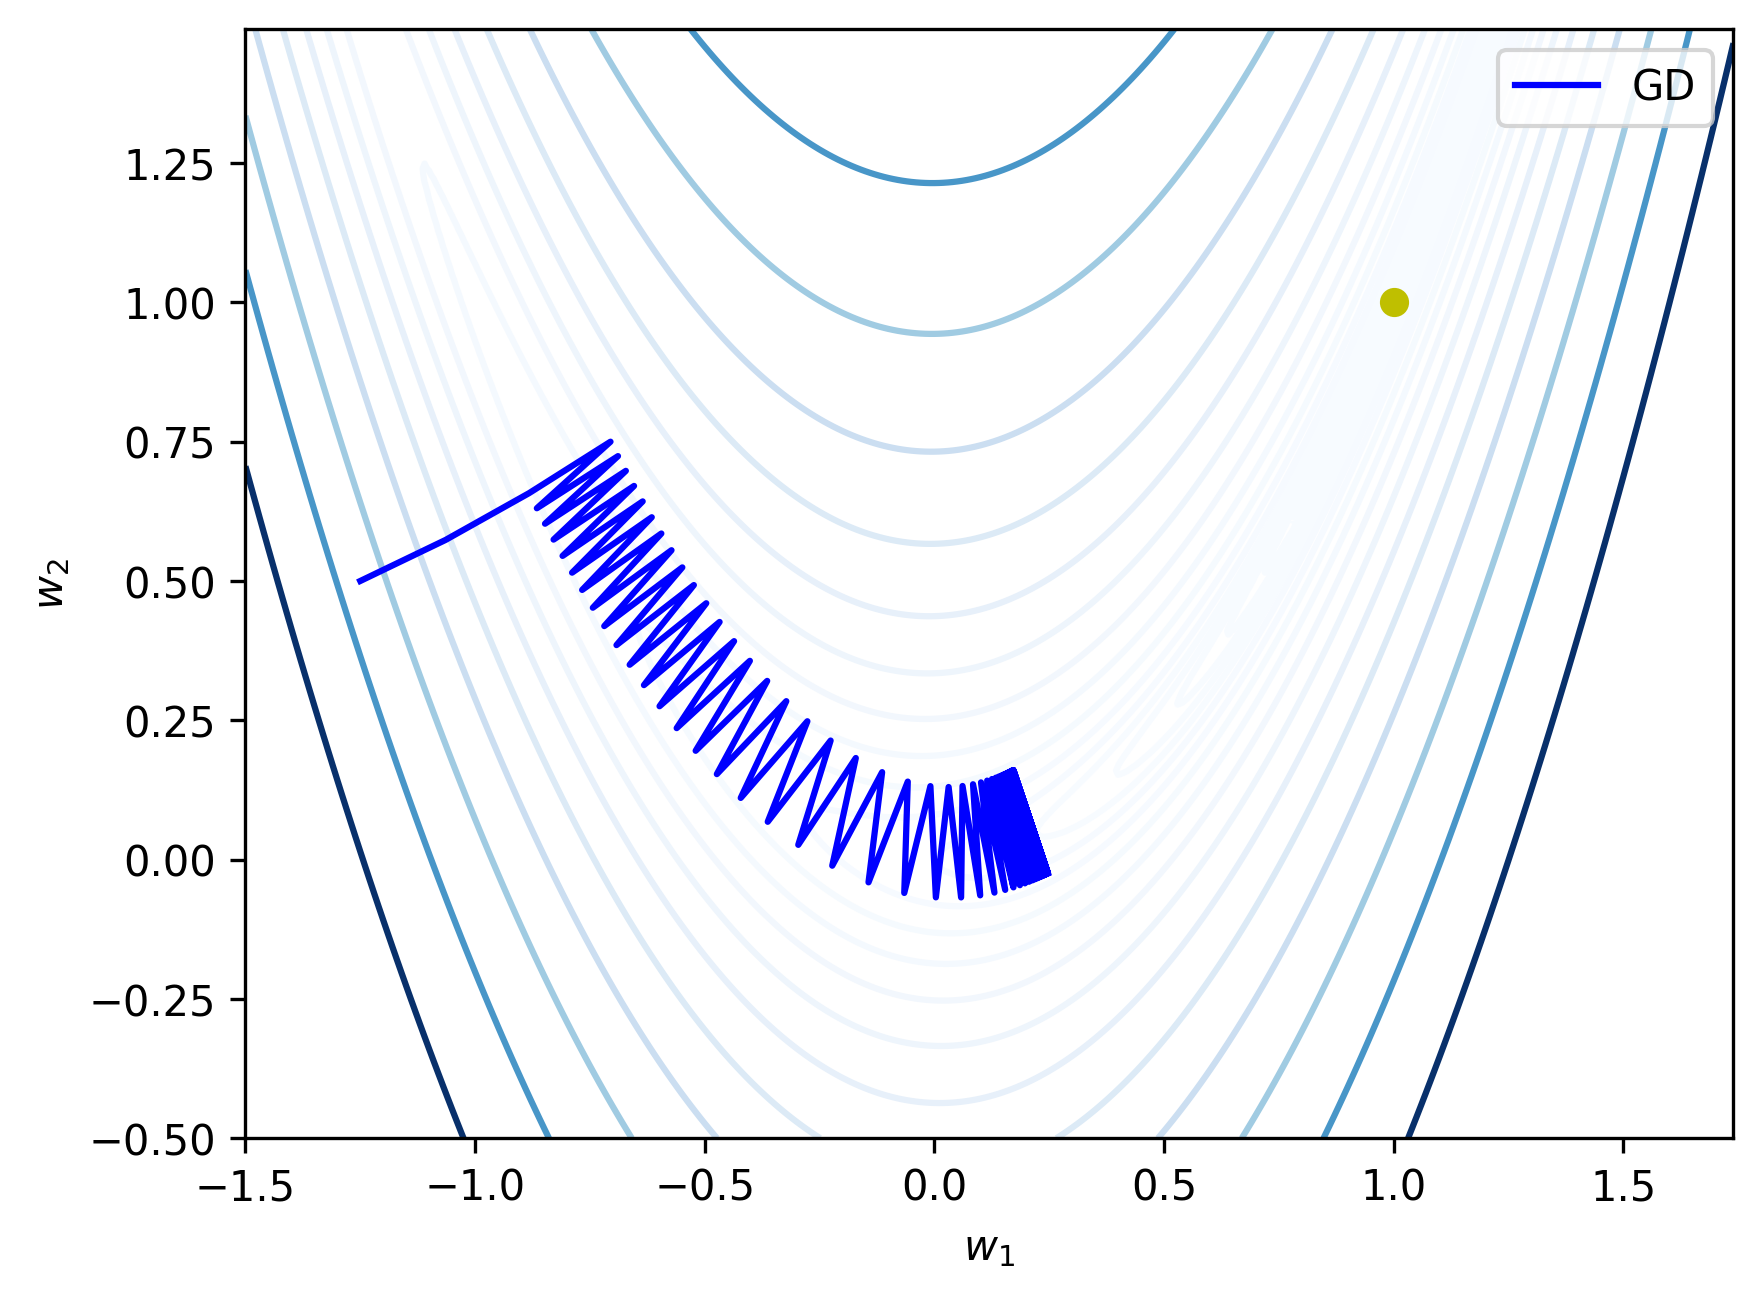
\includegraphics[width=0.6\linewidth]{chapters/neural/images/gd_oscillating.png}
	\caption{Работа градиентного спуска при минимизации функции Розенброка. Метод всегда шагает на фиксированное расстояние чтобы было видно осцилляции.}
	\label{img:gd_osc}
\end{figure}

На решение этих проблем и направлены различные эвристики и обобщения, которые мы рассмотрим далее.

\begin{problem}[Медленная сходимость градиентного спуска.]
Пусть минимизируемая функция имеет следующий вид: $\mathcal{L}(w, x) = (w - w^*)^T M (w - w^*)$, где $M \in \mathbb{R}^{m \times m}$~--- положительно определенная матрица с собственными числами $\lambda_1 = 1$, $\lambda_m = 10^{-4}$. Вычислите величину градиентного шага  $h$, при которой градиентный спуск с постоянным шагом будет гарантированно сходиться. Сколько при такой величине шага потребуется итераций для достижения требуемой точности $\varepsilon$, если точка старта $x_0 = v_m$, где $v_m$~--- собственный вектор матрицы $M$, соответствующий собственному числу $\lambda_m$ и имеющий единичную норму?
\end{problem}

\begin{remark}
Сценарий из этой задачи особенно части встречается, если не отнормировать данные перед обучением модели. 
\end{remark}

\subsection{Метод накопления инерции}

Чтобы избежать осцилляций и сделать стохастический градиентный спуск более плавным, можно добавить градиенту <<инерцию>>, и усреднять его значение по последним нескольким шагам. Тогда получится метод \textbf{Momentum}, или метод тяжелого шарика, изобретенный Б. Т. Поляком в 1964 г. Его метод обновления весов может быть записан так:
\begin{align*}
v &:= \gamma v + (1 - \gamma) \mathcal{L}'(w, x_i) \\
w &:= w - h v\,,
\end{align*}
где параметр $h$ отвечает за величину шага, а $\gamma$~--- за то, насколько сильно предыдущие итерации будет влиять на текущую.

Развил эту идею Ю. Е. Нестеров, в 1983 г. предложив метод \textbf{NAG} (Nesterov's accelerated gradient). В нём градиент не только усредняется по нескольким итерациям, но и <<подглядывает>> вперед в направлении своего движения, и обновляет веса с учетом полученной информации:
\begin{align*}
v &:= \gamma v + (1 - \gamma) \mathcal{L}'(w - h \gamma v, x_i) \\
w &:= w - h v\,,
\end{align*}

Эти методы хорошо показали себя при обучении больших нейросетевых моделей. По сравнению с стохастическим градиентным спуском они обладают большей устойчивостью к выбросам, меньше осциллируют.

\begin{figure}[h]
	\centering
	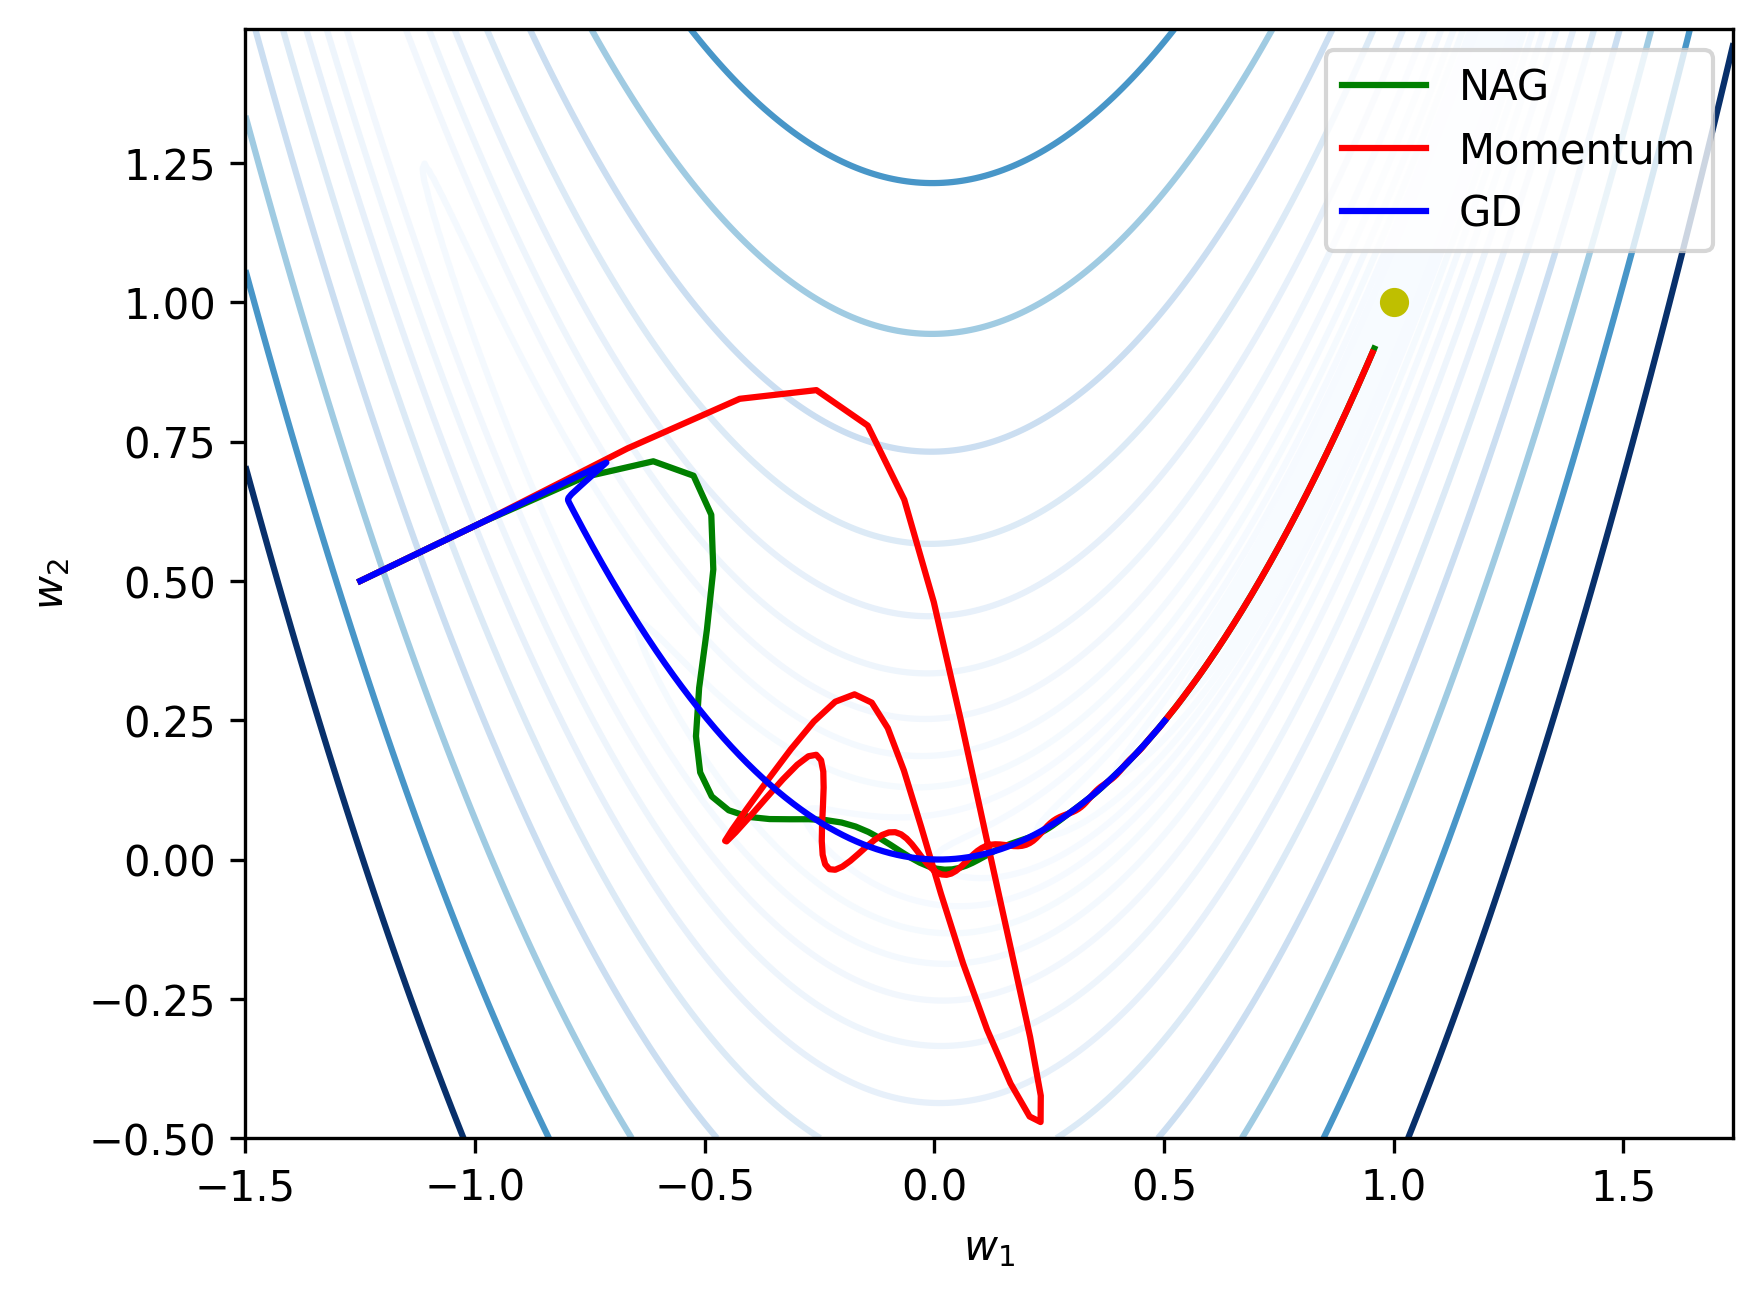
\includegraphics[width=0.6\linewidth]{chapters/neural/images/nag_momentum_gd.png}
	\caption{Пример работы методов Momentum, NAG и градиентного спуска при оптимизации функции Розенброка. Все методы делают $10^4$ итераций.}
	\label{img:gd_osc}
\end{figure}

\subsection{Варианты инициализации весов}

Чтобы улучшить сходимость метода можно правильно инициализировать веса модели. Возможно очень много различных вариантов, например:
\begin{enumerate}
    \item $w_j := 0$ для всех $j=1,\dots,n$;
    \item Небольшие случайные значения, $w_j := \text{random}\left(-\frac{1}{2n}, \frac{1}{2n}\right)$;
    \item Обучение по небольшой стартовой предвыборке объектов;
    \item Мультистарт: многократные запуски из различных случайных начальных приближений и выбор лучшего из них;
    \item В случае линейной регрессии, $w_j := \frac{\langle y, f_j \rangle}{\langle f_j, f_j \rangle}$, где $f_j = (f_j(x_i))_{i=1}^l$.
\end{enumerate}

\begin{problem}[Смысл 5 способа инициализации весов.]
Покажите что в модели линейной регрессии с квадратичной функцией потерь и некореллированными признаками ($\langle f_j, f_k \rangle = 0,\ j \neq k$), веса, полученные с помощью оценки 5 на самом деле являются точным решением задачи оптимизации.
\end{problem}

\subsection{Варианты порядка предъявления объектов}

Метод стохастического градиента чувствителен к тем способу предоставления новых оъектов на каждом шаге. Для улучшения сходимости можно применить одну из следующих эвристик:

\begin{enumerate}
    \item Перетасовка объектов (shuffling). Можно перемешивать объекты, брать попеременно объекты из разнвх классов. Это помогает избежать переобучения если объекты, например, хранятся в хронологическом порядке.
    \item Чаще брать объекты на которых функция потерь принимает большие значения. Это помогает нейросети выучить сложные примеры, даже если в выборке их немного.
\end{enumerate}

В задачах многоклассовой классификации также можно применять следующие техники:
\begin{enumerate}
    \item В задачах классификации чаще брать объекты на которых меньше уверенность (margin).
    \item Вообще не брать <<хорошие>> объекты на которых margin больше константы $\mu_+$. Это может ускорить сходимость.
    \item Вообще не брать объекты <<выбросы>> на которых margin меньше константы $\mu_-$. Это может улучшить качество классификации. 
\end{enumerate}
В этих случаях константы $\mu_+$ и $\mu_-$ придется подбирать.

\subsection{Варианты выбора градиентного шага}

Вообще говоря, сходимость метода стохастического градиента с фиксированным шагом это чудо~--- даже для выпуклых функций метод будет осциллировать в окрестности минимума. Чтобы бороться с проблемой осцилляций можно варьировать величину градиентного шага.

\begin{enumerate}
    \item Можно уменьшать величину шага с каждой итерацией. В таком случае для выпуклых функций сходимость гарантируется если:
    \[
    h_t \rightarrow 0,\, \sum_{t = 1}^{\infty} h_t = \infty,\, \sum_{t=1}^{\infty} h_t^2 < \infty
    \]
    В частности можно положить $h_t = 1 / t$.
    \item Можно на каждом шаге выбирать величину шага, минимизирующую функцию одной переменной:
    \[
    \mathcal{L}(w - h \nabla \mathcal{L}(w, x_i), x_i) \rightarrow \min_h\,.
    \]
    Это называется \textbf{метод скорейшего градиентного спуска}.
    \item Можно делать случайные <<пробные>> шаги, которые помогут <<выбить>> функцию из неглубокого локального минимума.
\end{enumerate}

\begin{figure}[h]
	\centering
	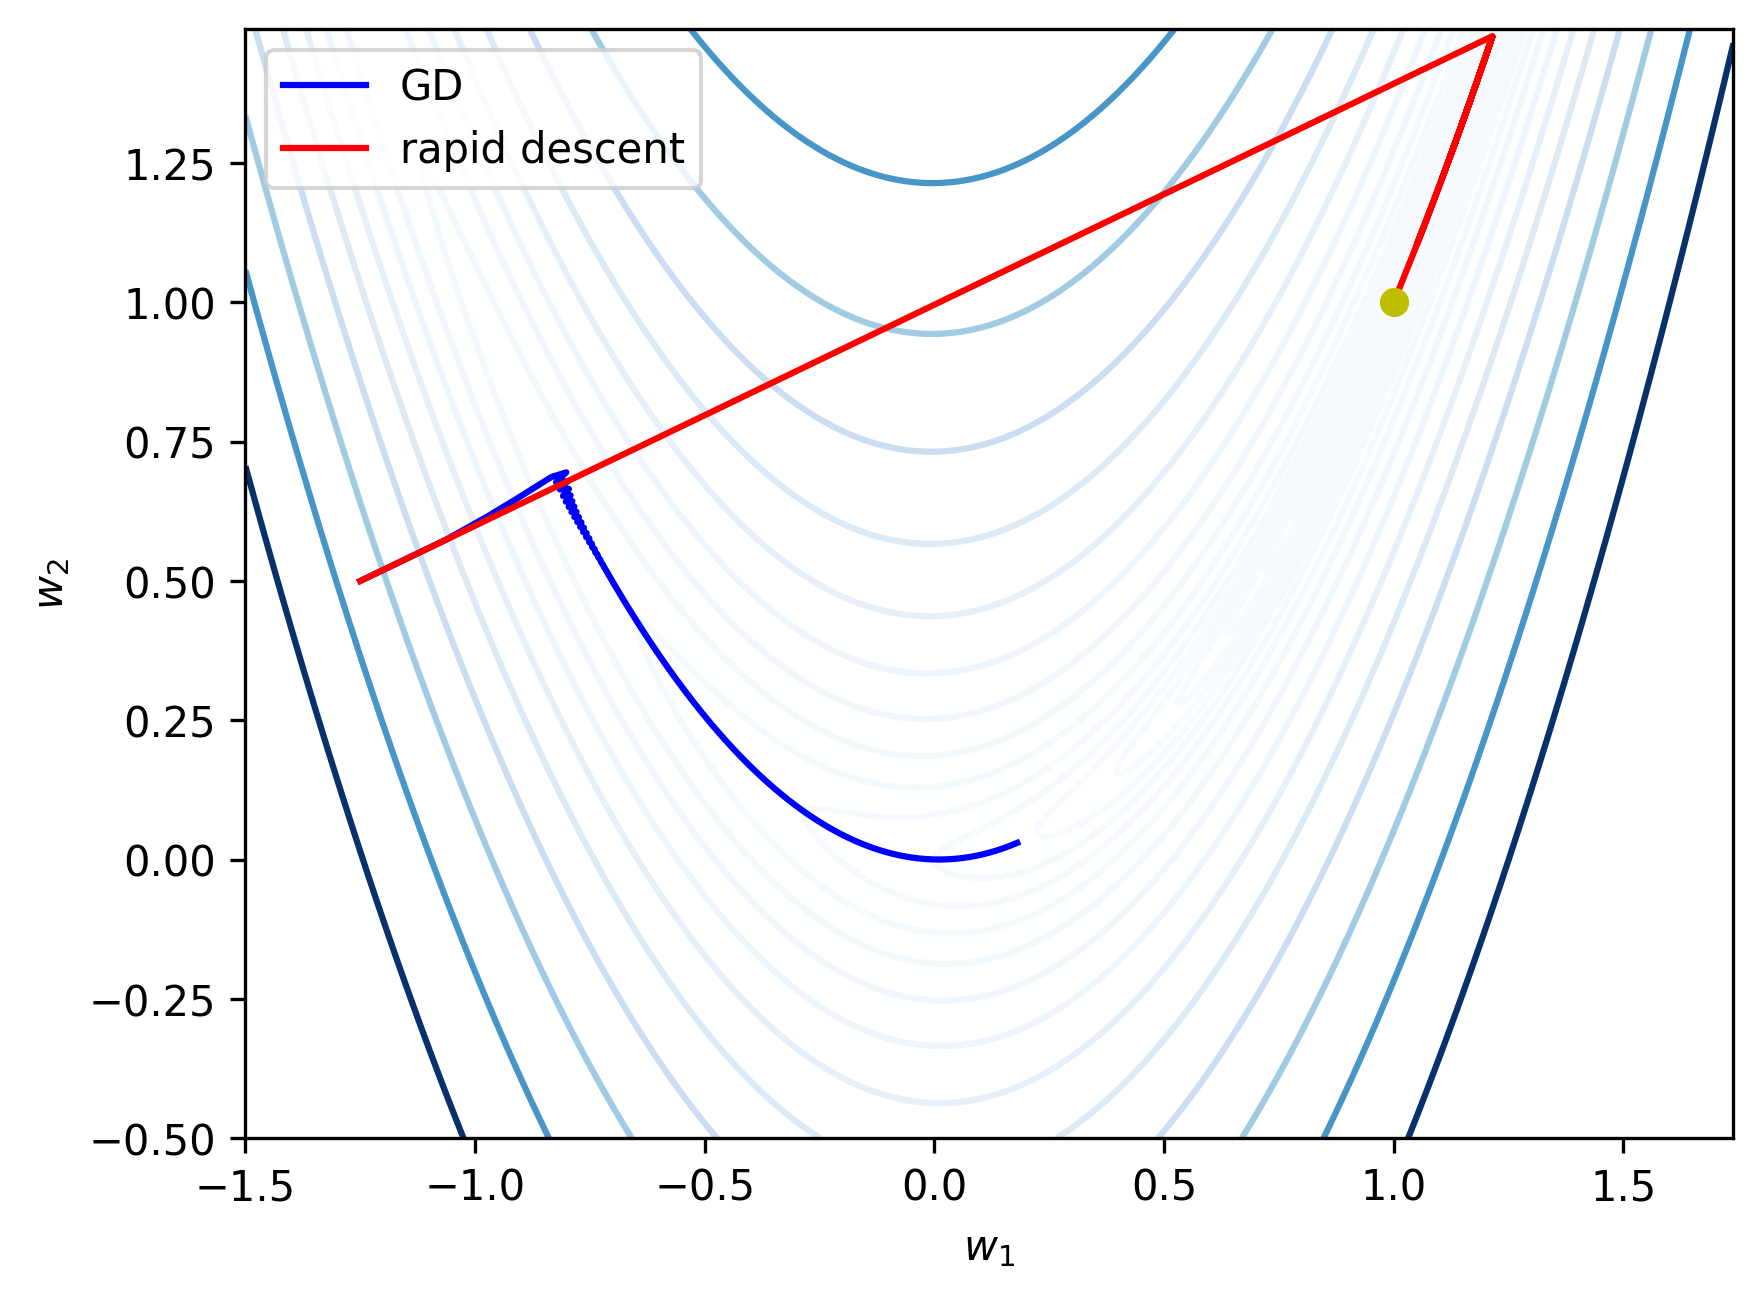
\includegraphics[width=0.6\linewidth]{chapters/neural/images/gd_rd_example.png}
	\caption{Работа градиентного спуска и скорейшего градиентного спуска при минимизации функции Розенброка. Оба метода делают $10^4$ итераций.}
	\label{img:gd_osc}
\end{figure}

\begin{remark}
Существуют и более продвинутые алгоритмы, модифицирующие величину градиентного шага, такие как Adagrad, RMSProp, Adadelta, а также методы, сочетающие идеи подстройки градиентного шага и накопления момента, такие как Adam, Adamax, Nadam. Часть их них будет рассмотрена в последующих параграфах.
\end{remark}

\subsection{Методы второго порядка}

Методы второго порядка используют не только градиент функции, но и ее гессиан. Это может дать очень хорошие результаты, например метод не будет застревать в седловых точках. Методы второго порядка предоставляют более быструю сходимость и точность ценой вычислительной эффективности, и в больших задачах они обычно не применяются.

Самый первый из методов второго порядка~--- многомерный метод Ньютона. Его итерацию можно записать как:
\[
w := w - \left(\nabla^2\mathcal{L}(w, x_i)\right)^{-1}\nabla \mathcal{L}(w, x_i)\,.
\]
Исходно метод Ньютона был предназначен для нахождения нуля функции, и выражение выше представляет собой просто-напросто метод для поиска нулей Гессиана. Однако в такой базовой формулировке метод очень часто расходится, и применятются его различные модификации, такие как метод Ньютона-Рафсона:
\[
w := w - h\left(\nabla^2\mathcal{L}(w, x_i)\right)^{-1}\nabla \mathcal{L}(w, x_i)\,.
\]
где $h$ может быть как постоянной, так и выбираться из соображений минимизации одномерной функции, как в методе скорейшего градиентного спуска.

Есть и огромное количество других обобщений, например метод Левенберга-Маквардта, который представляет собой суперпозицию методов Ньютона-Рафсона и обычного градиентного спуска.

\begin{problem}[Сравнение методов первого и второго порядков]
    Докажите, что если минимизируемая функция квадратична, $\mathcal{L}(w, x) = (w - w^*)^T M (w - w^*)$, где $M$~--- положительно определенная матрица, метод Ньютона сойдется к минимуму за одну итерацию. Сравните вычислительную алгоритма сложность с той, которую вы получили в первой задаче для $\varepsilon = 10^{-8}$
\end{problem}

\section{Функции активации ReLU и PReLU. Проблема «паралича» сети.}
\subsection{Про функции активации}

Функция активации в контексте нейронных сетей определяет выходной сигнал нейрона на основе входного сигнала или набора входных сигналов. Она играет важную роль в определении нелинейности модели и позволяет нейронной сети обучаться сложным зависимостям между входными данными и выходами, а также влияеть на эффективность обучения модели.(грубо говоря определяет будет ли нейрон активирован - даст не нулевой выход) \\
В искусственных нейронных сетях используются различные типы функций активации, такие как тождественная функция, ступенчатые функции, сигмоидные функции и многие другие. \\
\textbf{Важным требованием} к функции активации является ее нелинейность, чтобы нейронная сеть могла эффективно справляться с нетривиальными задачами.\\ Примером широко используемой функции активации является ReLU.

\subsection{ReLU (Rectified Linear Unit), проблема «паралича» сети}

\textbf{\textit{Определение:}} 
Функция активации ReLU определяется как:
$f(x) = max(0, x)$, где x — входное значение.\\
Не смотря на очевидную простоту функции активации ReLU, у неё есть одна существенная проблема: она может вызывать так называемый \textbf{«паралич» сети}.\\
Если градиент весов становится слишком большим, то некоторые нейроны могут получить очень большие отрицательные веса, что приведёт к тому, что их выходные значения всегда будут равны нулю независимо от входного сигнала. Эти нейроны становятся неактивными («замороженными») и больше не участвуют в процессе обучения. Если это происходит слишком часто, то это может привести к ухудшению результата.\\
Для решения этой проблемы была предложена модификация ReLU.
\subsection{PReLU (Parametric Rectified Linear Unit)}

\textbf{\textit{Определение:}}
Функция PReLU является обобщением ReLU и определяется как:
$$ f(x) = \begin{cases}
x & \text{if } x > 0 \\
\alpha x & \text{if } x \leq 0
\end{cases} $$
В отличие от обычной ReLU, где все отрицательные значения обнуляются, PReLU вводит дополнительный параметр $\alpha$, который управляет наклоном линии для отрицательных значений. Этот параметр $\alpha$ может быть обучен вместе с другими параметрами сети, что позволяет избежать полного отключения нейронов. То есть даже отрицательный входной сигнал будет вносить вклад в обучение модели, что уменьшает проблему паралича сети и улучшает получаемый результат.

\subsection{Задачи}
\textbf{Задача 1}

Представьте, что вы получили графики функций активации ReLU и PReLU (с заданным параметром $\alpha$) для различных входных значений.\\
Опишите, как выглядит график функции активации ReLU и как он отличается от графика PReLU. Какова роль параметра $\alpha$ в PReLU?\\
\textbf{Решение}

График функции ReLU выглядит как угол, который начинается от нуля и идет вверх с углом 45 градусов для положительных значений.\\
График функции PReLU (Parametric ReLU) также имеет две части, но для отрицательных значений он не обрезается до нуля. Вместо этого, он наклонен под углом, определяемым параметром $\alpha$. \\
Роль параметра $\alpha$ в PReLU:\\
Параметр $\alpha$ определяет наклон линии для отрицательных значений. Если $\alpha$ велико, то выход будет относительно большим даже для небольших отрицательных входов, что позволяет нейрону сохранять некоторую активность. Если $\alpha$ близко к нулю, то функция будет почти горизонтальной для отрицательных значений, что делает нейрон менее активным в этом диапазоне.\\
\textbf{Задача 2.1}

Рассмотрим простой случай использования функции активации ReLU в одном слое нейронной сети. Пусть входной сигнал равен $-4$, а вес этого нейрона равен $10$. Каково будет значение на выходе этого нейрона после применения функции активации ReLU?\\
\textbf{Решение:}

Выходной сигнал до применения функции активации будет равен произведению входа и веса: $-4 \cdot 10 = -40$. После применения функции активации ReLU получаем: $f(-40) = \max(0, -40) = 0$. Таким образом, этот нейрон станет неактивным ("замороженным"), поскольку его выходной сигнал всегда будет нулевым независимо от изменения входного сигнала.\\
\textbf{Задача 2.2}

Пусть теперь используется функция активации PReLU с параметром $\alpha = 0.01$. Рассчитайте значение на выходе того же нейрона, что и в предыдущей задаче, но уже с использованием PReLU.\\
\textbf{Решение:}

После умножения входа и веса получаем тот же результат: $-4 \cdot 10 = -40$. Теперь применяем функцию активации PReLU:

$$ f(-40) = \begin{cases}
-40 & \text{if } (-40) > 0 \\
0.01 \cdot (-40) & \text{if } (-40) \leq 0
\end{cases} $$

Так как $-40 \leq 0$, мы используем вторую часть определения функции: $f(-40) = 0.01 \cdot (-40) = -0.4$. В этом случае нейрон не становится полностью замороженным, так как его выходной сигнал остается отличным от нуля даже при отрицательном входе.\\
\textbf{Задача 3}

Входной сигнал $x$ распределён равномерно на интервале [-10, 10], а вес $w$ нейрона равен 2, параметр $\alpha = 0.1$.\\
Какова вероятность, что нейрон заморозится при использовании каждой из функций ReLU и PReLU?\\
\textbf{Решение:}\\
Для ReLU:\\
Нейрон «замораживается», если выходной сигнал после применения функции активации всегда равен нулю. То есть, если $wx <= 0$.\\
Поскольку $w = 2$, условие $wx <= 0$ эквивалентно $x <= 0$.\\
Вероятность того, что $x$ окажется меньше или равно нулю, равна вероятности того, что $x$ попадет в интервал -10, 0. \textit{Это составляет половину всего диапазона распределения, поэтому вероятность равна 0.5.}\\
При использовании PReLU нейрон никогда не «замерзнет», потому что даже при отрицательных значениях $x$ выходной сигнал будет отличен от нуля благодаря параметру $\alpha$.
\textit{Таким образом, вероятность того, что нейрон «заморозится», равна 0.}

\section{Drop Out}
\subsection{Теоретические сведения}

\textbf{Drop Out} (метод отключения случайных нейронов) - это метод, который представляет собой эффективный подход к борьбе с переобучением в полносвязных нейронных сетях. 

Переобучение может происходить, когда нейроны в сети начинают "запоминать" шум и особенности обучающего набора, вместо того чтобы извлекать общие закономерности. Во время обучения нейронной сети нейроны взаимодействуют друг с другом, и иногда происходит так, что один нейрон начинает исправлять ошибки другого. Это может привести к ситуации, когда в одном слое нейронов образуются большие веса с разными знаками, что делает модель менее стабильной и затрудняет ее обобщение. В таких случаях, даже если модель демонстрирует высокую точность на обучающих данных, она может оказаться неэффективной на тестовых данных.

Идея Drop Out заключается в том, что при обучении случайные нейроны отключаются (то есть возвращают всегда нулевое значение) и не участвуют в данном шаге обучения. В таком случае большие значения весов разных знаков не всегда участвуют в обучении одновременно, и модель стабилизируется.

Обучение с Dropout можно интерпретировать как обучение одновременно $2^N$ моделей (где $N$ ~--- количество нейронов) с разными архитектурами связей. При обучении выбирается модель, наиболее устойчивая к потере доли нейронов; разные части модели решают одну и ту же задачу вместо того, что бы компенсировать ошибки друг друга.

Недостатком Drop Out является более долгое обучение модели в связи со случайностью процесса обучения.

\subsection{Реализация}
При обучении выбирается параметр $p$ ~--- вероятность отключения. Модель обучается с отключением случайных нейронов. Можно отключать в каждом слое долю $p$ нейронов, вместо независимого отключения, чтобы избежать полного отключения одного слоя.

$$x_i^l = \xi_i^l \sum_{j=1}^{K_{l-1}} w_{ij}^l x_j^{l-1} $$

$l$ ~--- номер текущего слоя, $i$ ~--- номер нейрона в этом слое, $K_l$ ~--- кол-во нейронов в слое $l$, $\xi \sim Be(1-p)$ ~--- случайная величина, отвечающая за отключение.

$\left[\xi_i^l\right] = 1-p$, поэтому на этапе применения вводится нормировка:
$$x_i^l = (1-p) \sum_{j=1}^{K_{l-1}} w_{ij}^l x_j^{l-1} $$

Чаще используется \textbf{Inverted Drop Out} для простоты применения:

$$x_i^l = \frac{\xi_i^l}{1-p} \sum_{j=1}^{K_{l-1}} w_{ij}^l x_j^{l-1} $$
~--- при обучении;

$$x_i^l = \sum_{j=1}^{K_{l-1}} w_{ij}^l x_j^{l-1} $$
~--- при применении.

\subsection{Задачи}
\begin{description}
\item[\textbf{Задача 1}] 
    Какие по порядку величины должны быть ограничения на значения $p$, чтобы избежать отключения одного слоя целиком?
\item[\textbf{Решение:}] если в сети $L$ слоёв размерности $K$, то $p \sim (\frac{c}{L})^{1/K}. $
    Тогда вероятность отключения одного слоя $p^K = \frac{c}{L}; $ вероятность функционирования всех слоёв: $\sim (1-p^K)^L = (1-\frac{c}{L})^L \sim e^{-c}$.
    
    Если взять $c\sim 0.01$ , получим вероятность работы сети $\sim 99\%$.
    
    Если $L=4, K=10,$ то $p \sim 54\%$.

\

\item[\textbf{Задача 2}] 
    Сколько шагов обучения нужно провести, чтобы не осталось нейронов, которые были бы выкинуты на каждом шаге (то есть совсем не обучались)?

\item[\textbf{Решение:}] если в сети $N$ нейронов, то вероятность одному нейрону совсем не обучиться в течение $T$ итераций равна $p^T$. Тогда среднее число необученных нейронов равно $Np^T$. Из условия $Np^T<1$ получаем $T>-\log_{p}N = \frac{\ln N}{\ln \frac{1}{p}}$.



%%%%%%%%%%%%%%%%%%%%%%%%%%%%%%%%%%%%%%%%%%%%%%%%%%%%%%%%%%%%%%%%%%%%%%%%%%%%%%%%%%%%%%%%%%%%%%%%%%%%%%%%%%%%%%%%%%%%%%%%%%%%%%%%%%%%%%%%%%%%%%%%%%%%%%%%%%%%%%%%%%%%%%%%%%%%%%%%%%%%%%%%%%%%%%%%%%%%%%%%%%%%%%%%%%%%%%%%%%%%%%%%%%%
\section{Персептрон и модель Изинга}

Персептрон является одной из базовых моделей машинного обучения и может быть интерпретирован как аналог физических систем, в частности, неоднородной модели Изинга. 
Эти аналогии вдохновили развитие ограниченных машин Больцмана (RBM), которые минимизируют энергетическую функцию, что позволяет создавать более устойчивые модели машинного обучения.  

Пусть имеется решётка, на каждом узле которой $i = 1, \dots, N$ расположена дискретная переменная, принимающая одно из двух состояний: $s_i = +1$ или $s_i = -1$. Эти состояния удобно называть \textit{спинами} (или нейронами в контексте персептрона), где $s_i = +1$ соответствует спину вверх, а $s_i = -1$ — спину вниз. 
Взаимодействие отдельного нейрона с остальными нейронами можно выразить через энергетическую функцию:
\[
E[S] = - \sum_i B_i S_i -\sum_{\langle i j \rangle} J_{ij} S_i S_j,
\]
где:
\begin{itemize}
    \item $S_i \in \{-1, 1\}$ — состояние спина;
    \item $J_{ij}$ — коэффициенты взаимодействия;
    \item $B_i$ — внешнее поле.
\end{itemize}
Если в модели присутствует только первый член, то нейроны не взаимодействуют друг с другом, и модель решается тривиально. Второй член отвечает за взаимодействие между соседними нейронами. Обозначение $\langle i j \rangle$ означает, что сумма берётся по всем парам ближайших соседей в решётке.

В отличие от классической модели Изинга, где взаимодействия между спинами задаются фиксированными параметрами $B$ и $J$, в данном подходе (аналогия с полевой теорией Гинзбурга–Ландау) эти параметры являются обучаемыми. Их значения уточняются в процессе обучения нейронной сети.

В вероятностной интерпретации модель Изинга описывается распределением Гиббса:
\[
P(S) = \frac{1}{Z} e^{-\beta E},
\]
где $Z$ — статистическая сумма:
\[
Z = \sum_{\{S_i\}} e^{-\beta E},
\]
а $\beta$ — это обратная температура 
 + нормировка, $\beta = \frac{1}{k_B T}$. При 
$T\rightarrow0$: сеть ведет себя как дискретная оптимизация (модель Изинга).
При $T \rightarrow \infty$: сеть становится шумной, склонной к случайным состояниям.(См. задача.)

С другой стороны, \textbf{Формула активации для бинарного персептрона:}
\[
y = \mathrm{sign}\left(\sum_{i=1}^n w_i x_i + w_0\right),
\]
где:
\begin{itemize}
    \item $x_i$ — входной сигнал;
    \item $w_i$ — вес связи;
    \item $w_0$ — смещение (bias);
    \item $\mathrm{sign}$ — функция активации, возвращающая $+1$ или $-1$.
\end{itemize}

Здесь веса $w_i$ и сигналы $x_i$ можно рассматривать как аналоги $J_{ij}$ и $S_i$, а функция активации $\mathrm{sign}$ моделирует взаимодействие спинов в системе.

Энергетическая функция $E$ в модели Изинга может быть интерпретирована как функция потерь в персептроне:
\[
E = - \mathbf{w}^\top \mathbf{x},
\]
где $\mathbf{w}$ — вектор весов, а $\mathbf{x}$ — входной вектор.

Минимизация энергии в модели Изинга аналогична обучению персептрона, где цель состоит в подборе весов, минимизирующих ошибку классификации.

\subsection{Функции активации и их физический смысл}

Рассмотрим однослойную нейронную сеть размерности $N - 1$ во внутреннем слое с нейронами $s_i$ и одним выходным нейроном $s_1$. Пусть на вход подаётся вектор размерности $M$. В качестве функции активации на выходном нейроне часто используется гиперболический тангенс:
\[
\mathrm{tanh}(B) = \frac{e^{B} - e^{-B}}{e^{B} + e^{-B}}, \quad -B = w_0 + \sum_i w_i s_i.
\]

Как будет показано далее, его выбор связан не только с асимптотическим поведением и хорошими гладкими свойствами. 

Рассмотрим статистическую сумму невзаимодействующих нейронов, умноженную на единицу:
\[
Z[J] = \left.\sum_{\{s_i\}} e^{-B s_i} e^{J s_i} \right|_{J=0}, \quad s_i \in \{\pm 1\}.
\]
Средняя энергия статистических систем определяется как, оно же мат ожидание нейрона $s$ опрделеяется:
\[
\langle s \rangle = \frac{1}{Z} \frac{\partial}{\partial J} Z = \frac{1}{Z} \sum_{\{s_i\}} e^{-B s_i + J s_i} s_i \bigg|_{J=0} = \tanh(-B).
\]
Таким образом, гиперболический тангенс представляет собой среднюю энергию спиновой системы в модели Изинга и моделирует взаимодействие спинов с одной стороны, и с другой, представляет из себя функцию потерь $\mathcal{L}$  персептрона.

\subsubsection*{Распределение нейронов в сети}

Если состояния нейронов скрытого слоя $i \in [2, N]$ известны, они выражаются через компоненты входного вектора и веса модели:
\[
P(s_i) = \frac{1}{Z_i} \exp\left[ w_{0i} s_i + \sum_{j=1}^M w_{ij} s_i x_j \right].
\]
Тогда вероятностное распределение выходного нейрона $i = 1$ задаётся как:
\[
P(s_1 | s_2, s_3, \dots, s_N) = \frac{1}{Z_1} \exp\left[ s_1 \left( w_{01} + \sum_{i=2}^N w_{i1} s_i \right) \right].
\]

Полное вероятностное распределение выходного нейрона будет иметь вид:
\[
P(s_1) = P(s_1 | s_2, \dots, s_N) \prod_{i=2}^N P(s_i) = \frac{1}{\prod_{i=1}^N Z_i} \exp\left[ \sum_{i=1}^N w_{0i} s_i + \sum_{i,j=2}^{N,M} w_{ij} s_i x_j + s_1 \sum_{j=1}^M w_{ij} s_j \right].
\]

Запишем это в терминах модели Изинга:
\[
P(s_1) = \frac{1}{Z} \exp\left[-\sum_i B_i s_i - \sum_{i,j} J_{ij} s_i s_j \right],
\]
где $B_i$ — магнитное поле, а $J_{ij}$ — взаимодействие нейронов, которые выражаются через веса. В процессе обучения модели (backpropagation) задача состоит в определении значений $B_i$ и $J_{ij}$.
Нахождение распределения вероятностей в сети соответствует решению задачи минимизации энергии модели Изинга.

\subsection{Задачи}
\textbf{Задача 1:} Покажите, что вероятностная интерпретация модели Изинга связана с логистической регрессией.

\textbf{Решение:}
Логистическая регрессия основана на функции активации:
\[
\sigma(x) = P(y=1 | x) = \frac{1}{1 + e^{-E}}, \quad E = \mathbf{w}^\top \mathbf{x} + w_0.
\]

Для модели Изинга распределение вероятностей:
\[
P(S = 1) = \frac{e^{-E}}{e^{E} + e^{-E}} = \frac{1}{1+ e^{2E}} =  \sigma(-2E),\quad P(S = -1) = \sigma(2E).
\]
что аналогично модели логистической регрессии с сигмоидальной функцией вероятности.
\textbf{Задачи 2 - 3:}  
Модель весов \( W \) персептрона имеет специальную структуру:
\[
W = \text{Diag}(d_1, d_2, \dots, d_N) + \mathbf{x} \mathbf{x}^\top,
\]
где \( \text{Diag}(d_1, d_2, \dots, d_N) \) — диагональная матрица, а \( \mathbf{x} \mathbf{x}^\top \) — внешнее произведение входного вектора \( \mathbf{x} \). Энергия системы(она же функция потерь) определяется как:
\[
E = -\mathbf{s}^\top W \mathbf{s},
\]
где \( \mathbf{s} \in \{-1, +1\}^N \).

\begin{enumerate}
    \item Найти состояние \( \mathbf{s} \), минимизирующее энергию \( E \).
    \item Найдите общее условие на W, при котором система имеет как минимум два устойчивых состояния $s_1$ и $s_2$. 
\end{enumerate}

\textbf{Решение:}

1. \textbf{Минимум функции энергии:}

Энергия \( E \) принимает вид:
\[
E = -\mathbf{s}^\top \text{Diag}(d_1, \dots, d_N) \mathbf{s} - \mathbf{s}^\top (\mathbf{x} \mathbf{x}^\top) \mathbf{s}.
\]

Первый член:
\[
-\mathbf{s}^\top \text{Diag}(d_1, \dots, d_N) \mathbf{s} = -\sum_{i=1}^N d_i s_i^2.
\]
Так как \( s_i^2 = 1 \) для \( s_i \in \{-1, +1\} \), получаем:
\[
-\mathbf{s}^\top \text{Diag}(d_1, \dots, d_N) \mathbf{s} = -\sum_{i=1}^N d_i.
\]

Второй член:
\[
-\mathbf{s}^\top (\mathbf{x} \mathbf{x}^\top) \mathbf{s} = -(\mathbf{x}^\top \mathbf{s})^2.
\]

Таким образом, энергия принимает вид:
\[
E = -\sum_{i=1}^N d_i - (\mathbf{x}^\top \mathbf{s})^2.
\]

Энергия минимизируется, когда \( (\mathbf{x}^\top \mathbf{s})^2 \) максимально. Это достигается, если компоненты вектора \( \mathbf{s} \) сонаправлены с компонентами \( \mathbf{x} \). То есть:
\[
s_i = \text{sign}(x_i), \quad i = 1, \dots, N.
\]

2. \textbf{Устойчивые состояния:}

Поскольку \( W \) симметрична, энергия может быть минимизирована, если состояния \( \mathbf{s} \) совпадают с собственными векторами матрицы \( W \), соответствующими наименьшим собственным значениям.

\begin{itemize}
    \item Один собственный вектор — это \( \mathbf{x} \) с собственным значением \( \|\mathbf{x}\|^2  + \overline{d}\) (d - взвешенного диагонального элемента по направлению x),
    \item Остальные \( N-1 \) собственных значений равны диагональным элементам \( d_i \).
\end{itemize}

Если \( \|\mathbf{x}\|^2 \gg d_i \), то устойчивое состояние \( \mathbf{s} \) сонаправлено с \( \mathbf{x} \). Если \( d_i \) доминируют, состояние определяется диагональными элементами.

Кроме того, симметрия матрицы \( W \) означает, что если \( \mathbf{s}^* \) минимизирует энергию, то \( -\mathbf{s}^* \) тоже является решением, так как:
\[
E(-\mathbf{s}^*) = E(\mathbf{s}^*).
\]

\textbf{Задача*} 

1. Рассмотрим однослойную нейронную сеть с \( N \) нейронами в скрытом слое и одним выходным нейроном. На вход поступает вектор \( \mathbf{x} \in \mathbb{R}^M \), веса имеют случайные значения \( w_i \sim \mathcal{N}(0, \sigma^2) \), а функция активации на выходном нейроне задается как:
   \[
   s_\text{out} = f\left( \sum_{i=1}^N w_i \cdot s_i + w_0 \right),
   \]
   где \( f(x) = \mathrm{tanh}(\beta x), \beta = 1/T \).

Что произойдет с выходом \( s_\text{out} \) при \( T \to \infty \) и \( T \to 0 \), если считать, что активация тангенса моделирует энергетическое состояние спиновой системы? 

2. Рассмотрим предельный случай, когда число нейронов \( N \to \infty \), а веса \( w_i \) независимы и одинаково распределены. Покажите, что результатирующее распределение выхода \( s_\text{out} \) будет стремиться к гауссовскому. В каком случае это приближение применимо?

\textbf{Решение:}

\subsubsection*{1. Поведение нейронной сети при \( T \to \infty \) и \( T \to 0 \)}

\textbf{При \( T \to \infty \):}
Гиперболический тангенс \( \mathrm{tanh}(\beta x) \) стремится к линейной функции:
\[
\mathrm{tanh}(\beta x) \approx \beta x \quad \text{при } \beta \to 0 \, (T \to \infty).
\]
Нейронная сеть теряет нелинейность, и выход становится линейной комбинацией входов:
\[
s_\text{out} \approx \beta \left( \sum_{i=1}^N w_i s_i + w_0 \right).
\]
Поведение сети приближается к \textbf{линейной модели}.

\textbf{При \( T \to 0 \):}

Гиперболический тангенс становится почти пороговой функцией:
\[
\mathrm{tanh}(\beta x) \to 
\begin{cases} 
-1, & x < 0, \\ 
1, & x > 0.
\end{cases}
\]
Нейронная сеть превращается в \textbf{дискретную систему}, где выходные значения строго определяются знаком линейной комбинации входов:
\[
s_\text{out} = \text{sign} \left( \sum_{i=1}^N w_i s_i + w_0 \right).
\]

\subsubsection*{2. Гауссовское распределение при \( N \to \infty \)}

\textbf{При} \( N \to \infty \), веса \( w_i \) независимы и одинаково распределены (\( w_i \sim \mathcal{N}(0, \sigma^2) \)), а входы \( s_i \in \{-1, 1\} \).
Сумма выходов на входном слое:
\[
S = \sum_{i=1}^N w_i s_i.
\]
По центральной предельной теореме:
\begin{itemize}
    \item Среднее \( \mu = \mathbb{E}[S] = 0 \) (поскольку \( \mathbb{E}[w_i] = 0 \) и \( \mathbb{E}[s_i] = 0 \)).
    \item Дисперсия \( \sigma^2 = N \cdot \mathbb{V}[w_i] \cdot \mathbb{V}[s_i] = N \sigma^2 \).
\end{itemize}
При \( N \to \infty \), \( S \) стремится к распределению:
\[
S \sim \mathcal{N}(0, N \sigma^2).
\]
Это верно при конечном $T$, Активация 
$\tanh$ сжимает значение $z \in [-1, 1]$, поскольку функция гладкая, форма распределения не меняется и зависит от двух моментов.
%%%%%%%%%%%%%%%%%%%%%%%%%%%%%%%%%%%%%%%%%%%%%%%%%%%%%%%%%%%%%%%%%%%%%%%%%%%%%%%%%%%%%%%%%%%%%%%%%%%%%%%%%%%%%%%%%%%%%%%%%%%%%%%%%%%%%%%%%%%%%%%%%%%%%%%%%%%%%%%%%%%%%%%%%%%%%%%%%%%%%%%%%%%%%%%%%%%%%%%%%%%%%%%%%%%%%%%%%%%%%%%%%%%


\section{CNN. Свёртки и пулинги для обработки изображений.}
\subsection{Стандартная схема свёрточной сети.}

$ x[i, j] $ — исходные признаки, пиксели $ n \times m $-изображения

$ w_{ab} $ — ядро свёртки, $ a = -A, \ldots, +A $, $ b = -B, \ldots, +B $

Неполносвязный свёрточный нейрон с $ (2A + 1)(2B + 1) $ весами:

$$
(x * w)[i, j] = \sum_{a=-A}^{A} \sum_{b=-B}^{B} w_{ab} \, x[i + a, j + b]
$$

Объединяющий нейрон — это необучаемая свёртка с шагом $ h > 1 $, агрегирующая данные прямоугольной области $ h \times h $(объединяющий слой нейронов = пулинг слой):

$$
y[i, j] = F \left( x[hi, hj], \ldots, x[hi + h - 1, hj + h - 1] \right)
$$

где  F  — агрегирующая функция: max, average и т.п. Max-pooling позволяет обнаружить элемент в любой из ячеек.

\begin{figure}[h]

\centering

\includegraphics[width=0.2\linewidth]{chapters/neural/images/пуллинг.png}

\label{fig:pulling}

\end{figure}

\begin{figure}[h]

\centering

\includegraphics[width=0.8\linewidth]{chapters/neural/images/1CNN.png}

\label{fig:one_cnn}

\end{figure}

Свёрточная сеть обучается извлечению признаков

Чем выше слой, тем более крупные и сложные элементы изображений он способен распознавать

\newpage
\subsection{Приложения CNN.}

Классификация изображений( Свёрточная сеть \textbf{AlexNet} )\\

Распознавание речевых сигналов\\
\begin{figure}[h]

\centering

\includegraphics[width=0.8\linewidth]{chapters/neural/images/pic.png}

\label{fig:voice_signals_nn}

\end{figure}

Классификация предложений в тексте:\\
Последовательные слова в тексте представляются векторами с помощью векторных представлений (word2vec и др.)\\

\newpage
\subsection{Обобщение CNN на любые структурированные данные.}
Допустим, каждый объект имеет структуру, заданную графом

\textbf{Свёртка} определяется по локальной окрестности вершины

\textbf{Пулинг} агрегирует векторы вершин локальной окрестности

Такая сеть обучается находить и классифицировать подграфы

\begin{figure}[h]

\centering

\includegraphics[width=0.8\linewidth]{chapters/neural/images/обобщениеCNN.png}

\label{fig:cnn_generalization}

\end{figure}

\subsection{Задачи}
\textbf{Задача 1}

Дано изображение размером 5x5 пикселей и свёрточное ядро размером 3x3 пикселя\\

\begin{equation*}
\begin{Vmatrix}
1 & 2 & 3 & 0 & 1\\
4 & 5 & 6 & 1 & 0\\
7 & 8 & 9 & 2 & 1\\
0 & 1 & 2 & 3 & 4\\
1 & 0 & 1 & 0 & 1
\end{Vmatrix}
""
\begin{Vmatrix}
1 & 0 & -1\\
1 & 0 & -1\\
1 & 0 & -1
\end{Vmatrix}
\end{equation*}
Необходимо выполнить операцию свёртки\\
\textbf{Решение}

1.Результирующая матрица после свёртки будет размером
$$ (5-3+1) \times (5-3+1) = 3 \times 3 $$.

2. Процесс свёртки:

Для каждого положения свёрточного ядра на изображении вычисляем\\
сумму произведений.

Позиция (0,0):
$
(1 \times 1) + (2 \times 0) + (3 \times -1) + \\
(4 \times 1) + (5 \times 0) + (6 \times -1) + \\
(7 \times 1) + (8 \times 0) + (9 \times -1) = \\
1 + 0 - 3 + 4 + 0 - 6 + 7 + 0 - 9 = -6
$

 Позиция (0,1):
$
(2 \times 1) + (3 \times 0) + (0 \times -1) + \\
(5 \times 1) + (6 \times 0) + (1 \times -1) + \\
(8 \times 1) + (9 \times 0) + (2 \times -1) = \\
2 + 0 + 0 + 5 + 0 - 1 + 8 + 0 - 2 = 12
$

Позиция (0,2):
$
(3 \times 1) + (0 \times 0) + (1 \times -1) + \\
(6 \times 1) + (1 \times 0) + (2 \times -1) + \\
(9 \times 1) + (2 \times 0) + (1 \times -1) = \\
3 + 0 - 1 + 6 + 0 - 2 + 9 + 0 - 1 = 16
$

Позиция (1,0):
$
(4 \times 1) + (5 \times 0) + (6 \times -1) + \\
(7 \times 1) + (8 \times 0) + (9 \times -1) + \\
(0 \times 1) + (1 \times 0) + (2 \times -1) = \\
4 + 0 - 6 + 7 + 0 - 9 + 0 + 0 - 2 = -6
$

Позиция (1,1):
$
(5 \times 1) + (6 \times 0) + (1 \times -1) + \\
(8 \times 1) + (9 \times 0) + (2 \times -1) + \\
(1 \times 1) + (0 \times 0) + (3 \times -1) = \\
5 + 0 - 1 + 8 + 0 - 2 + 1 + 0 - 3 = 8
$

Позиция (1,2):
$
(6 \times 1) + (1 \times 0) + (0 \times -1) + \\
(9 \times 1) + (2 \times 0) + (1 \times -1) + \\
(2 \times 1) + (3 \times 0) + (4 \times -1) = \\
6 + 0 + 0 + 9 + 0 - 1 + 2 + 0 - 4 = 12
$

Позиция (2,0):
$
(7 \times 1) + (8 \times 0) + (9 \times -1) + \\
(0 \times 1) + (1 \times 0) + (2 \times -1) + \\
(1 \times 1) + (0 \times 0) + (3 \times -1) = \\
7 + 0 - 9 + 0 + 0 - 2 + 1 + 0 - 3 = -4
$

Позиция (2,1):
$
(8 \times 1) + (9 \times 0) + (2 \times -1) + \\
(1 \times 1) + (2 \times 0) + (3 \times -1) + \\
(0 \times 1) + (1 \times 0) + (4 \times -1) = \\
8 + 0 - 2 + 1 + 0 - 3 + 0 + 0 - 4 = 0
$

Позиция (2,2):
$
(9 \times 1) + (2 \times 0) + (1 \times -1) + \\
(2 \times 1) + (3 \times 0) + (4 \times -1) + \\
(1 \times 1) + (0 \times 0) + (1 \times -1) = \\
9 + 0 - 1 + 2 + 0 - 4 + 1 + 0 - 1 = 6
$

После выполнения всех операций свёртки\\
мы получаем следующую матрицу:

$$
\begin{Vmatrix}
-6 & 12 & 16 \\
-6 & 8 & 12 \\
-4 & 0 & 6 \\
\end{Vmatrix}
$$

\newpage
\textbf{Задача 2}

Даны изображения продукции с производственной линии.\\
К сожалению, некоторые с дефектами.\\
Предоставьте алгоритм построения CNN для распознавания дефектов на изображениях.

\textbf{Подойдёт такое решение:}

\begin{enumerate}
    \item Создать CNN с тремя свёрточными слоями и двумя pooling-слоями.
    \item Использовать dropout для предотвращения переобучения.
    \item Добавить полносвязный слой перед выходным слоем.
    \item Взять сигмоидный выходной слой для бинарной классификации.
    \item Обучить модель на размеченных изображениях, используя функцию потерь бинарная кросс-энтропия.\end{enumerate}\\

\textbf{Задача 3}

Каковы основные компоненты CNN и их функции?\\
\textbf{Решение:}
\begin{itemize}
    \item Свёрточные слои: применяют свёртку к входным данным, чтобы выделить важные признаки.
    \item Слои подвыборки(Pooling): уменьшают размерность данных, сохраняя наиболее значимую информацию.
    \item Полносвязные слои: используются для окончательной классификации на основе извлечённых признаков.
\end{itemize}

\end{description}


\section*{Оптимальное прореживание нейронных сетей}

\subsection*{Введение}
Прореживание нейронных сетей (англ. optimal brain damage) — метод упрощения структуры регрессионной модели, например, нейронной сети. Основная идея прореживания (англ. pruning) заключается в том, что те элементы модели или те нейроны сети, которые оказывают малое влияние на ошибку аппроксимации, можно исключить из модели без значительного ухудшения качества аппроксимации \cite[VorontsovOptBrainDamage].
Такой подход позволяет достичь следующих целей:
\begin{itemize}
    \item \textbf{Сжатие нейросети.} Уменьшается количество параметров, которые нужно хранить, что важно для устройств с ограниченными ресурсами.
    \item \textbf{Ускорение вычислений.} Меньшее количество параметров требует меньше операций умножения, что ускоряет работу модели.
    \item \textbf{Регуляризация.} Снижение числа параметров уменьшает склонность модели к переобучению, делая её более устойчивой к шуму данных.
    \item \textbf{Повышение качества.} Часто итоговая модель после прореживания показывает лучшие результаты, чем исходная.
    Это связано с тем, что избыточно сложная модель склонна к переобучению, а последовательное исключение избыточных параметров позволяет оптимально адаптировать её сложность к задаче.
\end{itemize}

\subsection*{История метода}
Метод второго порядка был предложен Яном ЛеКуном в 1990 году \cite{lecun1990optimal} и получил название \textit{Optimal Brain Damage}.
На тот момент этот подход был одним из лучших для уменьшения размеров нейронных сетей и улучшения их качества.
Позднее Хассиби и Штурм \cite{hassibi1993optimal} разработали его улучшение \textit{Optimal Brain Surgery}, основываясь на анализе вторых производных. 
Ранее существовали методы нулевого порядка, где исключались элементы с малыми весами \cite{mozer1989skeletonization}.
В 1990 году А. Н. Горбань предложил метод, использующий первые производные, что позволило обойтись без вычисления вторых производных. 
Этот подход получил название \textit{контрастирование нейронных сетей}. Е. М. Миркес развил идеи Горбаня, создав библиотеку функций и язык описания для проекта «Идеального нейрокомпьютера».

Впоследствии появились более современные методы, например Dropout, $L_2$-регуляризация и другие, которые вытеснили этот подход из основного арсенала.
Тем не менее, метод прореживания всё ещё может быть полезным инструментом, особенно в ситуациях, требующих компактности модели.

\subsection*{Математическая постановка задачи}
Рассмотрим регрессионную модель 
\[
y_n = f(\mathbf{w}, \mathbf{x}_n) + \nu,
\]
где $\mathbf{w} \in \mathbb{R}^d$ — вектор параметров, $\mathbf{x}_n \in \mathbb{R}^p$ — вектор независимых переменных, $y_n \in \mathbb{R}$ — зависимая переменная, $\nu$ — случайная ошибка. 

Задана выборка $D = \{(\mathbf{x}_n, y_n)\}_{n=1}^N$. Для минимизации функции ошибки 
\[
E_D(\mathbf{w}) = \sum_{n=1}^N \ell(y_n, f(\mathbf{w}, \mathbf{x}_n)),
\]
где $\ell(\cdot, \cdot)$ — функция потерь, требуется найти $\mathbf{w}^{MP} = \arg\min_{\mathbf{w}} E_D(\mathbf{w})$. 

\subsection*{Прореживание параметров}
Цель метода — исключение параметров $w_i$, которые оказывают наименьшее влияние на ошибку $E_D$.
Для этого используется квадратичная аппроксимация $E_D$ в окрестности $\mathbf{w}^{MP}$:
\[
E_D(\mathbf{w} + \Delta\mathbf{w}) \approx E_D(\mathbf{w}^{MP}) + \frac{1}{2} \Delta\mathbf{w}^T H \Delta\mathbf{w},
\]
где $H = \nabla^2_{\mathbf{w}} E_D(\mathbf{w}^{MP})$ — матрица Гессе.

Исключение параметра $w_i$ эквивалентно наложению ограничения $\Delta w_i + w_i = 0$.
Для выполнения данного условия минимизируется функция:
\[
\Delta E_D = \frac{1}{2} \Delta\mathbf{w}^T H \Delta\mathbf{w},
\]
при ограничении $\mathbf{e}_i^T \Delta\mathbf{w} + w_i = 0$, где $\mathbf{e}_i$ — единичный вектор с $i$-м элементом, равным $1$. 

\subsection*{Оптимизация}
Используем метод множителей Лагранжа для минимизации:
\[
S = \frac{1}{2} \Delta\mathbf{w}^T H \Delta\mathbf{w} - \lambda (\mathbf{e}_i^T \Delta\mathbf{w} + w_i).
\]
Дифференцируя $S$ по $\Delta\mathbf{w}$ и $\lambda$ и приравнивая производные к нулю, получаем:
\[
\Delta\mathbf{w} = -\frac{w_i}{[H^{-1}]_{ii}} H^{-1} \mathbf{e}_i.
\]
Подставляя это выражение в $\Delta E_D$, находим:
\[
L_i = \frac{w_i^2}{2 [H^{-1}]_{ii}}.
\]
Параметр $i$, минимизирующий $L_i$, выбирается для исключения.

\subsection*{Итеративный процесс прореживания}
Вышенаписанный процесс можно повторять несколько раз для повышения эффиктивности модели:
\begin{enumerate}
    \item Определяется вес, который оказывает минимальное влияние на ошибку, и он исключается из модели.
    Удаление выполняется до тех пор, пока ошибка не превышает заданный порог.
    \item После удаления части параметров модель дообучается, чтобы восстановить её качество.
    \item Процесс повторяется, пока не будет достигнута желаемая компактность или качество модели или пока не пройдет заданное число итераций.
\end{enumerate}

\subsection*{Задачи}
\begin{task}
Выпишите Лагранжиан для решения задачи нахождения веса, зануление которого ведет к минимальной ошибке для методов 3 и 4 порядков. Попробуйте решить эту оптимизационную задачу.
\end{task}

\begin{task}
Мы раскладываем функции ошибки до второй производной, хотя приращение $\Delta w_i = -w_i$ может быть достаточно большим. Оцените применимость данного метода в зависимости от величины весов $w_i$.
\end{task}

\begin{task}
Рассчитайте $L_i$ для модели, в которой $H = \begin{bmatrix} 4 & 2 \\ 2 & 3 \end{bmatrix}$, $w = \begin{bmatrix} 1 \\ -2 \end{bmatrix}$.
\end{task}

\section{Batch normalization}

\subsection{Введение}
В основе Batch Normalization лежит решение проблемы «внутреннего ковариационного сдвига» (Internal Covariate Shift). Этот термин описывает явление, при котором распределение входных данных каждого слоя нейронной сети меняется в процессе обучения, из-за чего сети становится сложнее обучать. Это происходит из-за того, что параметры предыдущих слоев изменяются во время обучения, влияя на данные текущего слоя.

Batch Normalization решает эту проблему, нормализуя выход каждого слоя. Нормализация заключается в преобразовании входных данных каждого слоя таким образом, чтобы среднее значение было приближено к нулю, а стандартное отклонение — к единице. Это делает сеть менее чувствительной к масштабу входных данных и улучшает общую стабильность процесса обучения.

Причина популярности batch normalization заключается в значительном ускорении обучения нейронных сетей и в улучшении их сходимости в целом. Его использование гарантирует, что каждая компонента представления на выходе будет иметь контролируемое среднее и дисперсию.

\subsection{Алгоритм}
Сперва идёт слой batch normalization, на котором текущий батч приводится к нулевому среднему и единичной дисперсии, где $\mu$ и $\sigma^2$ - среднее и дисперсия признаков по обрабатываемому батчу, $\varepsilon$ - гиперпараметр слоя, служащий для численной устойчивости.

\[X^{k+1} = \frac{X^k - \mu}{\sqrt{\sigma^2 + \varepsilon}}\]

Далее идёт слой channelwise scaling, который позволяет выучить оптимальное шкалирование для всех признаков $X^{k+2}$. Где $beta$ и $\gamma$ - обучаемые параметры, позволяющие настраивать в ходе обучения оптимальные значения матожидания и дисперсии выходного слоя.

\[X^{k+2} = \beta X^{k+1} + \gamma \]

В ходе предсказания мы используем $\mu_*$ $\sigma_*^2$, полученные в ходе обучения как скользящее среднее всех средних и дисперсий. 

\subsection{Задачи}

\subsubsection*{Задача 1}
Рассмотрим ситуацию: у вас есть небольшой набор данных, и мини-батчи содержат только по 2-3 образца. Какие проблемы могут возникнуть при использовании Batch Normalization в таких условиях? Какие методы можно использовать для решения этих проблем?

\subsubsection*{Задача 2}
Как параметры скользящих статистик влияют на работу модели?

\subsubsection*{Задача 3}
Почему нельзя использовать статистики конкретного батча во время предсказания


\section{Методы оптимизации с использованием Autograd: SGD, Adam, RMSProp}

\subsection{Автоматическое дифференцирование с Autograd}

Autograd \textendash{} это инструмент для автоматического дифференцирования, который позволяет автоматически вычислять градиенты функций. В контексте методов оптимизации, Autograd упрощает процесс нахождения производных для сложных функций потерь. Благодаря Autograd, пользователю не нужно вручную выводить градиенты \textendash{} они вычисляются программно с использованием обратного распространения (backpropagation).

Autograd используется во многих популярных библиотеках, таких как \texttt{PyTorch} и \texttt{JAX}. На семинарах были продемонстрированы примеры использования Autograd для автоматического вычисления градиентов при оптимизации нейронных сетей.

\subsubsection{Пример использования Autograd}

Предположим, у нас есть функция потерь $L(\theta) = (\theta^2 + 3\theta + 2)$. С помощью Autograd можно вычислить градиент этой функции по параметру $\theta$:

\begin{verbatim}
import autograd.numpy as np
from autograd import grad

def loss(theta):
    return theta**2 + 3 * theta + 2

grad_loss = grad(loss)
print(grad_loss(1.0))  # Выводит 5.0
\end{verbatim}

\subsection{Стохастический градиентный спуск (SGD)}

Стохастический градиентный спуск (SGD) представляет собой метод оптимизации, который используется для минимизации функции потерь $L(\theta)$, где $\theta$ \textendash{} параметры модели. На каждом шаге обновления параметров SGD использует оценку градиента по одному или нескольким случайно выбранным объектам:

\begin{equation}
\theta_{t+1} = \theta_t - \eta \nabla_\theta L_i(\theta_t),
\end{equation}

где:
\begin{itemize}
    \item $\theta_t$ \textendash{} параметры на шаге $t$;
    \item $\eta$ \textendash{} коэффициент обучения;
    \item $\nabla_\theta L_i(\theta_t)$ \textendash{} градиент функции потерь по $i$-му примеру на шаге $t$.
\end{itemize}

SGD часто используется благодаря своей простоте, но он может быть неустойчивым и медленным при выборе неподходящего коэффициента обучения.

\subsection{RMSProp}

Метод RMSProp (Root Mean Square Propagation) предназначен для адаптивного изменения шага обучения. В отличие от SGD, RMSProp учитывает среднеквадратичное значение градиентов для каждого параметра. Формулы для обновления параметров имеют вид:

\begin{align}
    g_t &= \nabla_\theta L_i(\theta_t), \\
    v_t &= \gamma v_{t-1} + (1 - \gamma) g_t^2, \\
    \theta_{t+1} &= \theta_t - \frac{\eta}{\sqrt{v_t + \epsilon}} g_t,
\end{align}

где:
\begin{itemize}
    \item $v_t$ \textendash{} скользящее среднее квадратов градиентов;
    \item $\gamma$ \textendash{} коэффициент сглаживания (обычно $0.9$);
    \item $\epsilon$ \textendash{} небольшая константа для избежания деления на ноль.
\end{itemize}

\subsection{Adam}

Метод Adam (Adaptive Moment Estimation) сочетает идеи из SGD и RMSProp, используя как первую, так и вторую моменты градиентов. Алгоритм Adam вычисляется по следующим формулам:

\begin{align}
    g_t &= \nabla_\theta L_i(\theta_t), \\
    m_t &= \beta_1 m_{t-1} + (1 - \beta_1) g_t, \\
    v_t &= \beta_2 v_{t-1} + (1 - \beta_2) g_t^2, \\
    \hat{m}_t &= \frac{m_t}{1 - \beta_1^t}, \\
    \hat{v}_t &= \frac{v_t}{1 - \beta_2^t}, \\
    \theta_{t+1} &= \theta_t - \frac{\eta}{\sqrt{\hat{v}_t} + \epsilon} \hat{m}_t,
\end{align}

где:
\begin{itemize}
    \item $m_t$ \textendash{} скользящее среднее градиентов (первая производная);
    \item $v_t$ \textendash{} скользящее среднее квадратов градиентов (вторая производная);
    \item $\beta_1$ и $\beta_2$ \textendash{} коэффициенты экспоненциального сглаживания (обычно $\beta_1 = 0.9$ и $\beta_2 = 0.999$);
    \item $\hat{m}_t$ и $\hat{v}_t$ \textendash{} корректированные моменты с учётом смещения;
    \item $\eta$ \textendash{} шаг обучения.
\end{itemize}

\subsection{Задачи}

\subsubsection*{Задача 1}
Рассмотрим функцию потерь $L(\theta) = \theta^2$. Используя SGD с шагом обучения $\eta = 0.1$, выполните два шага оптимизации, начиная с $\theta_0 = 1$. Найдите $\theta_1$ и $\theta_2$.

\textbf{Решение:}
\begin{align*}
    \nabla_\theta L(\theta_0) &= 2 \cdot \theta_0 = 2 \cdot 1 = 2, \\
    \theta_1 &= \theta_0 - 0.1 \cdot 2 = 1 - 0.2 = 0.8, \\
    \nabla_\theta L(\theta_1) &= 2 \cdot 0.8 = 1.6, \\
    \theta_2 &= \theta_1 - 0.1 \cdot 1.6 = 0.8 - 0.16 = 0.64.
\end{align*}

\subsubsection*{Задача 2}
Покажите, что в RMSProp, если градиент на каждом шаге постоянен и равен $g$, значение $v_t$ стремится к $g^2$ при $t \to \infty$.

\textbf{Решение:}
\begin{align*}
    v_t &= \gamma v_{t-1} + (1 - \gamma) g^2.
\end{align*}

В установившемся режиме $v_t = v_{t-1} = v$, поэтому:
\begin{align*}
    v &= \gamma v + (1 - \gamma) g^2, \\
    v (1 - \gamma) &= (1 - \gamma) g^2, \\
    v &= g^2.
\end{align*}

\subsubsection*{Задача 3}
Докажите, что для Adam корректированные моменты $\hat{m}_t$ и $\hat{v}_t$ стремятся к $m_t$ и $v_t$ соответственно при $t \to \infty$.

\textbf{Решение:}
\begin{itemize}
    \item $\hat{m}_t = \frac{m_t}{1 - \beta_1^t}$. При $t \to \infty$, $\beta_1^t \to 0$, поэтому $1 - \beta_1^t \to 1$ и $\hat{m}_t \to m_t$.
    \item Аналогично, $\hat{v}_t = \frac{v_t}{1 - \beta_2^t}$, и при $t \to \infty$, $\hat{v}_t \to v_t$.
\end{itemize}

\section{LSTM и GRU}

\subsection{LSTM. Основная идея}

\begin{figure}[h]
	\centering
	\includegraphics[width=0.6\linewidth]{chapters/neural/images/lstm.png}
	\caption{Схема LSTM}
	\label{img:lstm}
\end{figure}
Основная идея LSTM~\cite{hochreiter1997long} --- использование механизма \textbf{ячейки памяти} и набора \textbf{затворов (gates)}, которые регулируют, какая часть информации из предыдущих шагов будет запоминаться, забываться и выводиться на выход. Это позволяет LSTM ``удерживать'' важную информацию на более длинных промежутках.

\subsection{Структура LSTM-ячейки}
В классической LSTM-ячейке три затвора:
\begin{enumerate}
    \item \textbf{Forget gate} (затвор забывания) управляет тем, какая часть предыдущего состояния памяти $C_{t-1}$ будет \textit{забыта}.
    \item \textbf{Input gate} (затвор записи) определяет, какая часть нового кандидата состояния $\tilde{C}_t$ попадёт в текущее состояние памяти.
    \item \textbf{Output gate} (затвор выхода) определяет, какая часть текущего состояния памяти $C_t$ будет подана на выход $h_t$.
\end{enumerate}

Типичные формулы (безbias-термов):
\[
f_t = \sigma(W_f \cdot [h_{t-1}, x_t]), \quad
i_t = \sigma(W_i \cdot [h_{t-1}, x_t]), \quad
\tilde{C}_t = \tanh(W_C \cdot [h_{t-1}, x_t]),
\]
\[
C_t = f_t \odot C_{t-1} + i_t \odot \tilde{C}_t,
\]
\[
o_t = \sigma(W_o \cdot [h_{t-1}, x_t]), \quad
h_t = o_t \odot \tanh(C_t).
\]

\subsection{Продвинутые моменты LSTM}
\begin{itemize}
    \item \textbf{Bidirectional LSTM}: двунаправленная архитектура для учёта контекста слева и справа.
    \item \textbf{Stacked LSTM}: многослойные (глубокие) LSTM для повышения выразительности.
    \item \textbf{Dropout и Recurrent Dropout}: регуляризация занулением нейронов в связях.
    \item \textbf{Attention Mechanisms}: совмещение с механизмом внимания (Attention) для более гибкого «фокуса» на нужных шагах входной последовательности.
\end{itemize}

\subsection{Архитектура GRU}

\begin{figure}[h]
	\centering
	\includegraphics[width=0.6\linewidth]{chapters/neural/images/gru.png}
	\caption{Схема GRU}
	\label{img:gru}
\end{figure}
GRU (Gated Recurrent Unit) была предложена в работе~\cite{cho2014properties} как упрощение по сравнению с LSTM: используется всего два затвора (update и reset), что уменьшает число параметров модели.

\subsection{Структура GRU-ячейки}
\begin{enumerate}
    \item \textbf{Update gate} $z_t$ управляет тем, сколько информации из предыдущего выхода $h_{t-1}$ перенести в новое состояние.
    \item \textbf{Reset gate} $r_t$ определяет, сколько ``старой'' информации нужно сбросить перед вычислением текущего кандидата.
\end{enumerate}

Основные формулы:
\[
z_t = \sigma(W_z \cdot [h_{t-1}, x_t]), \quad
r_t = \sigma(W_r \cdot [h_{t-1}, x_t]),
\]
\[
\tilde{h}_t = \tanh \bigl(W_h \cdot [r_t \odot h_{t-1}, x_t]\bigr),
\]
\[
h_t = (1 - z_t)\odot h_{t-1} + z_t \odot \tilde{h}_t.
\]

\subsection{Преимущества GRU}
\begin{itemize}
    \item Меньше параметров по сравнению с LSTM, что может ускорять обучение.
    \item Часто качество на задачах NLP и временных рядах сопоставимо с LSTM.
\end{itemize}

\subsection{Продвинутые моменты GRU}
\begin{itemize}
    \item \textbf{Layer Normalization / BatchNorm}: нормализация на выходе или по слоям помогает стабилизировать обучение.
    \item \textbf{Residual/Skip Connections}: добавляются короткие связи для улучшения обратного распространения ошибки.
    \item \textbf{Bidirectional GRU}: аналогично двунаправленным LSTM, учитываем контекст с двух сторон.
\end{itemize}

\subsection{Сравнение LSTM и GRU}
\begin{itemize}
    \item LSTM имеет более гибкую структуру (три затвора, отдельное состояние $C_t$), но и больше параметров.
    \item GRU проще, часто обучается быстрее и даёт сравнимое качество.
\end{itemize}


\subsection{Теоретическая Задача 1: Анализ взрывающих и затухающих градиентов}
Объясните, почему в классической RNN (без затворов) возникает проблема затухающих и взрывающих градиентов при обучении на длинных последовательностях. Как архитектуры LSTM и GRU помогают смягчить эту проблему?

\begin{itemize}
    \item \textbf{Классическая RNN} использует повторяющиеся умножения весовых матриц на каждом временном шаге. Для длинных цепочек такие последовательные умножения могут привести к экспоненциальному затуханию или экспоненциальному росту (взрыв градиентов), поскольку собственные значения матриц многократно перемножаются.
    \item \textbf{LSTM и GRU} вводят механизмы затворов и явные пути прямой передачи градиента (``гейтированные'' или ``прямые'' связи через состояние), что существенно стабилизирует процесс обучения. Ячейка памяти LSTM (и аналогичная структура в GRU) создаёт путь, по которому градиент может проходить без постоянного перемножения на матрицу весов. Таким образом, модели меньше страдают от затухания или взрыва.
\end{itemize}

\subsection{Теоретическая Задача 2: Сравнение количества параметров в LSTM и GRU}
Предположим, что размерность входа равна $d$, а размер скрытого состояния равен $h$. Сравните (количественно) число обучаемых параметров в одной LSTM-ячейке и одной GRU-ячейке. Объясните, как это влияет на время обучения и возможность переобучения?

\begin{itemize}
    \item \textbf{LSTM} имеет 4 вычислительных ``ветви'' (forget, input, candidate, output), каждая включает матрицу весов для входа $W_{*}^{(x)}$ и для предыдущего скрытого состояния $W_{*}^{(h)}$, а также соответствующие bias. Итого для LSTM:
    \[
    \text{Параметры в LSTM} \approx 4 \cdot (d \cdot h + h \cdot h + h)
    \]
    \item \textbf{GRU} имеет 3 ветви (update, reset, candidate), что даёт формулу:
    \[
    \text{Параметры в GRU} \approx 3 \cdot (d \cdot h + h \cdot h + h)
    \]
    \item Таким образом, GRU имеет меньше параметров, что может приводить к более быстрой сходимости и меньшей склонности к переобучению (но и менее ``гибкой'' архитектуре в некоторых случаях).
\end{itemize}

\subsection{Теоретическая Задача 3: Пределы LSTM/GRU при очень длинных зависимостях}

Поясните, в каких случаях даже LSTM или GRU могут не справляться с очень длинными зависимостями? Предложите, какие механизмы или архитектуры способны улучшить качество работы с подобными зависимостями.

\begin{itemize}
    \item \textbf{Очень длинные зависимости}: даже с механизмами затворов для очень больших длин (например, сотни или тысячи временных шагов) LSTM/GRU могут всё ещё сталкиваться с трудностями в запоминании самых первых шагов. 
    \item \textbf{Mechanisms/архитектуры}: 
    \begin{itemize}
        \item \textbf{Attention} (применение в Encoder-Decoder архитектурах). Позволяет модели ``обращаться'' к нужным шагам напрямую, минуя долгую цепочку рекуррентных состояний.
        \item \textbf{Transformers}: полностью отказываются от рекуррентной структуры и используют механизм внимания (self-attention), что улучшает способность моделировать дальние зависимости.
        \item \textbf{Memory-augmented networks} (Neural Turing Machines, Memory Networks): явное внешнее хранилище.
    \end{itemize}
\end{itemize} 

\section{KAN как альтернативная базовая архитектура}
\subsection{Теорема Коллмогорова Арнольда}

В области машинного обучения многослойные персептроны (MLP) традиционно считаются универсальными аппроксиматорами функций. Однако существует менее известный, но не менее важный математический результат - теорема Колмогорова-Арнольда, которая предлагает альтернативный подход к представлению многомерных функций.
Теорема Колмогорова-Арнольда, доказанная в 1957 году, утверждает, что любая непрерывная функция нескольких переменных может быть представлена как суперпозиция непрерывных функций одной переменной и операции сложения. Формально это можно записать следующим образом:
\[
f(x_1, ..., x_n) = \sum_{q=1}^{2n+1} \Phi_q \left(\sum_{p=1}^n \phi_{q,p}(x_p)\right)
\]
где $\phi_{q,p}$ и $\Phi_q $ - непрерывные функции одной переменной.

Долгое время теорема Колмогорова-Арнольда считалась преимущественно теоретическим результатом без практического применения. Основная причина заключалась в том, что функции $\phi_{q,p}$ и $\Phi_q$ могут быть очень сложными и даже разрывными, что делает их непрактичными для численной реализации.

\subsubsection{Теоретическая задача 1: представление Колмогорова-Арнольда}
Приведите функцию $ f(x,y,z) = \frac{x^y}{z} $ в виде представления Колмогорова-Арнольда

\textbf{Решение:}
\[
f(x,y,z) = \frac{x^y}{z} = \exp(\exp(\log y + \log \log x) + (-\log z))
\]
\[
\Phi_1 = \exp
\]
\[
\phi_{1, 1} = \exp\log(y)
\]
\[
\phi_{1, 2} = \log\log(y)
\]
\[
\phi_{1, 3} = -\log z
\]

\subsection{Kolmogorov-Arnold Networks (KAN)}

Теорема Колмогорова-Арнольда вдохновила создание нового класса нейронных сетей - сетей Колмогорова-Арнольда (KAN), которые предлагают альтернативу традиционным многослойным персептронам. В то время как MLP используют фиксированные функции активации на узлах ("нейронах"), KAN размещает обучаемые функции активации на рёбрах ("весах") и реализует их с помощью B-сплайнов.
B-сплайны представляют собой кусочно-полиномиальные функции, обладающие рядом важных свойств:
\begin{itemize}
    \item Локальность: изменение одного контрольного узла влияет только на ограниченную область функции
    \item Гладкость: B-сплайны обеспечивают заданную степень непрерывности производных
    \item Компактность: эффективное представление сложных функций с небольшим числом параметров
\end{itemize}

Формально, слой KAN с входной размерностью $n_{in}$ и выходной размерностью $n_{out}$ можно определить как матрицу одномерных функций:
\[
\Phi(X) = {\phi_{q,p}}, p = 1,2,\ldots,n_{in}, q = 1,2,\ldots,n_{out}
\]
где каждая функция $\phi_{q,p}$ параметризована как B-сплайн с обучаемыми коэффициентами.

Главным отличием от исходной теоремы в KAN является уход от фиксированной глубины. Полная нейронная сеть представляет из себя композицию слоёв, то есть последовательное применение функциональных матриц:
\[
KAN(X) = \Phi_n(\Phi_{n - 1}( ...\Phi_2(\Phi_1(X))...))
\]

Исследования показывают, что KAN могут достигать сравнимой или лучшей точности по сравнению с более крупными MLP при использовании значительно меньшего количества параметров. Например, для решения дифференциальных уравнений в частных производных двухслойная KAN шириной 10 может быть в 100 раз точнее и в 100 раз эффективнее по параметрам, чем четырехслойная MLP шириной 100.

\subsubsection{Теоретическая задача 2: сети Колмогорова-Арнольда}
Покажите, как использовать обратное распространениие ошибки для обучения KAN.

\textbf{Решение:}

Использование B-сплайна в определении слоя затрудняет прямое применение обратного распространения ошибки, так как его производная в каждой точке заранее неизвестна. Однако каждый B-сплайн можно заменить на скрытый слой из перцептронов с одним входом и разными функциями активации, соответствующими базисным функциям сплайна, производные которых известны заранее. Таким образом KAN сводится к традиционной нейронной сети.

\subsection{КАН для обучения без учителя}

Сети Колмогорова-Арнольда могут быть эффективно адаптированы для задач обучения без учителя, что открывает новые возможности для анализа данных и научных открытий. В отличие от традиционного применения в задачах обучения с учителем, KAN для обучения без учителя фокусируются на поиске скрытых зависимостей в данных без явного указания целевых переменных.
Основная идея заключается в преобразовании задачи обучения без учителя в специальную форму обучения с учителем. Пусть имеется набор признаков $(x_1, x_2, ..., x_d)$, среди которых предполагается наличие функциональных зависимостей. Цель состоит в поиске нетривиальной функции $f$, такой что:
\[
f(x_1, x_2, ..., x_d) \approx 0
\]

Для решения этой задачи используется контрастивный подход, где определяются:
Позитивные примеры: реальные наборы признаков
Негативные примеры: наборы признаков с случайной перестановкой значений

KAN обучается различать эти два класса примеров, используя специальную модификацию архитектуры с гауссовой функцией активации в последнем слое:
\[
KAN_{unsupervised}(X) = \delta (KAN(X)), \text{ где } \delta(x) = \exp(-\frac{x^2}{2w^2})
\]
Такой подход позволяет KAN автоматически обнаруживать нетривиальные зависимости в данных. Например, в физических экспериментах сеть может выявлять фундаментальные законы природы, анализируя только измеренные величины.

\subsubsection{Теоретическая задача 3: KAN без учителя}
Какой датасет и какая архитектура KAN нужна для переоткрытия второго закона Ньютона?

\textbf{Решение:}

Набор данных должен содержать следующие измерения:
\begin{itemize}
    \item массы тел (m)
    \item приложенных сил (F)
    \item наблюдаемых ускорений (a)
\end{itemize}

Выражение меняется на:
\[
F=ma\rightarrow F-ma=0
\]
Далее представим это выражение в виде KAN:
\[
KAN(F, m, a) = \delta\left( F-\exp\left( \log m + \log a \right) \right),
\]
\[
\text{ где } \exp, \log \text{ - B-сплайны, определяемые во время обучения}
\]
Для обучения настоящие данные будут иметь целевую переменную равную 1, а случайно созданные - 0. Полученные в результате обучения функции позволят получить правильный вид закона.



\begin{thebibliography}{99}
\bibitem{hochreiter1997long} S.~Hochreiter, J.~Schmidhuber, \textit{Long short-term memory.} Neural Computation, 9(8), 1735--1780, 1997.
\bibitem{cho2014properties} K.~Cho, B.~van Merrienboer, D.~Bahdanau, Y.~Bengio, \textit{On the properties of neural machine translation: Encoder-decoder approaches.} arXiv preprint arXiv:1409.1259, 2014.
\end{thebibliography}

\section*{Быстрые методы стохастического градиента: Поляка и Нестерова}

Методы ускорения градиентного спуска применяются для уменьшения количества итераций, необходимых для достижения минимума функции потерь. Два важных метода для ускорения сходимости — это метод накопления инерции (Momentum) Поляка и метод ускоренного градиента Нестерова.


\subsection*{Метод Поляка (Momentum)}

Метод Поляка использует понятие \textit{накопленной скорости} для сглаживания обновления параметров и уменьшения колебаний. Вместо прямого шага в направлении градиента, метод учитывает предыдущие обновления. Формулы метода:

\begin{equation*}
\begin{aligned}
    v &:= \gamma v + (1 - \gamma) \nabla \mathcal{L}(w, x_i), \\
    w &:= w - \eta v,
\end{aligned}
\end{equation*}
где $\gamma \in [0, 1)$ — коэффициент импульса, $\eta$ — шаг обучения, $\nabla \mathcal{L}(w, x_i)$ — градиент функции потерь для $x_i$, $v$ — накопленная скорость.

Таким образом, метод Поляка комбинирует текущий градиент с предыдущими направлениями движения, что позволяет "разгоняться" в одном направлении и сглаживать траекторию на плоских участках.

\subsection*{Метод Нестерова (Nesterov Accelerated Gradient, NAG)}

Метод Нестерова представляет собой модификацию метода Поляка, где используется идея предварительного "предсказания" положения параметров. Основное отличие в том, что градиент рассчитывается не в текущей точке, а в точке, смещённой в направлении скорости. Формулы обновления параметров:
\begin{equation*}
\begin{aligned}
    v &:= \gamma v + (1 - \gamma) \nabla \mathcal{L}(w - \eta \gamma v, x_i), \\
    w &:= w - \eta v.
\end{aligned}
\end{equation*}

"Заглядывание вперёд" в направлении текущей скорости позволяет более точно учитывать геометрию функции и улучшать сходимость. Это позволяет методу Нестерова минимизировать колебания и снижать избыточные шаги в направлении градиента.

\subsection*{Графическое объяснение методов}

\begin{figure}[h!]
    \centering
    \begin{minipage}[t]{0.45\textwidth}
        \centering
        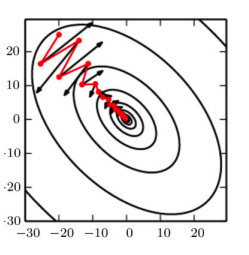
\includegraphics[width=0.9\textwidth]{chapters/neural/images/polyak.png}
        \\[0.5em]
        Рис. 1: Метод Поляка (Momentum)
    \end{minipage}%
    \hfill
    \begin{minipage}[t]{0.45\textwidth}
        \centering
        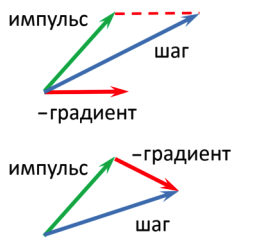
\includegraphics[width=0.9\textwidth]{chapters/neural/images/nesterov.png}
        \\[0.5em]
        Рис. 2: Метод Нестерова (NAG)
    \end{minipage}
\end{figure}

\begin{itemize}
    \item На левом рисунке показано, как метод Поляка сглаживает путь оптимизации за счёт накопленного импульса.
    \item На правом рисунке метод Нестерова использует "предсказание" положения параметров, что приводит к более оптимальному шагу.
\end{itemize}

\subsection*{Сравнение методов}
    \item - Метод Поляка прост в реализации и хорошо работает на негладких функциях.

    \item - Метод Нестерова обеспечивает более высокую скорость сходимости благодаря использованию информации о кривизне.

    \item - Оба метода легко интегрируются в современные алгоритмы оптимизации, такие как Adam и RMSProp.

\subsection*{Задача 1}
Рассмотрим функцию
\[
f(w) = w^2.
\]
Примените метод градиентного спуска с импульсом Поляка для минимизации этой функции. Шаг обучения $\eta = 0.1$, коэффициент импульса $\gamma = 0.9$, начальная точка $w_0 = 5$. Выполните три итерации.

\textbf{Решение:}

\[
v_t = \gamma v_{t-1} + (1 - \gamma) \nabla f(w_t), \quad w_{t+1} = w_t - \eta v_t,
\]
где $v_t$ — накопленная скорость, $\nabla f(w_t)$ — градиент функции $f(w) = w^2$, а $\eta$ — шаг обучения.

1.
   \[
   w_0 = 5, \quad v_0 = 0, \quad \nabla f(w_0) = 2w_0 = 10.
   \]
   \[
   v_1 = 0.9 \cdot 0 + (1 - 0.9) \cdot 10 = 1, \quad w_1 = 5 - 0.1 \cdot 1 = 4.9.
   \]

2.
   \[
   w_1 = 4.9, \quad \nabla f(w_1) = 9.8.
   \]
   \[
   v_2 = 0.9 \cdot 1 + (1 - 0.9) \cdot 9.8 = 1.88, \quad w_2 = 4.9 - 0.1 \cdot 1.88 = 4.712.
   \]

3.
   \[
   w_2 = 4.712, \quad \nabla f(w_2) = 9.424.
   \]
   \[
   v_3 = 0.9 \cdot 1.88 + (1 - 0.9) \cdot 9.424 = 2.634, \quad w_3 = 4.712 - 0.1 \cdot 2.634 = 4.448.
   \]

\textbf{Ответ:} после трёх итераций метода Поляка значение параметра $w$ уменьшилось с 5 до $4.448$ - он движется в сторону минимума функции $f(w) = w^2$.

\subsection*{Задача 2}
Для функции 
\begin{equation*}
    f(w) = (w - 3)^2 + 7
\end{equation*}
выполните две итерации метода Нестерова с параметрами $\eta = 0.2$ и $\gamma = 0.8$, начиная с $w = -1$. Найдите значения $w$ после каждой итерации.

\textbf{Решение:}
\begin{equation*}
    v_k = \gamma v_{k-1} + (1 - \gamma) \nabla f(w_k - \eta \gamma v_{k-1}), \quad w_{k+1} = w_k - \eta v_k.
\end{equation*}
1.
\[
   w_0 = -1, \quad v_0 = 0, \quad \nabla f(-1) = 2(-1 - 3) = -8.
\]
\[ v_1 = 0.8 \cdot 0 + 0.2 \cdot (-8) = -1.6, \quad w_1 = -1 - 0.2 \cdot (-1.6) = -0.68. \]
2. 
\[
   w_1 = -0.68, \quad v_1 = -1.6, \quad \nabla f(-0.68 - 0.2 \cdot 0.8 \cdot (-1.6)) = -6.848.
\]
\[ v_2 = 0.8 \cdot (-1.6) + 0.2 \cdot (-6.848) = -2.08, \quad w_2 = -0.68 - 0.2 \cdot (-2.08) = -0.272. \]

\textbf{Ответ:} после двух итераций значение $w$ изменилось с $-1$ до $-0.272$.

\subsection*{Задача 3}
Рассмотрим функцию:  
 \item\( f_1(w) = 10w_1^2 + w_2^2 \) (вытянутая квадратичная функция)   

Предположим, что для минимизации используется либо метод Поляка (Momentum), либо метод Нестерова (NAG).  
\item Начальная точка: \( w_0 = (10, 5) \),  шаг обучения \( \eta = 0.1 \),   коэффициент импульса \( \gamma = 0.9 \).  

Укажите, какой метод будет эффективнее и почему.

\textbf{Решение:}

1. Градиенты в направлении \( w_1 \) (\( \nabla_{w_1} f = 20w_1 \)) гораздо больше, чем в направлении \( w_2 \) (\( \nabla_{w_2} f = 2w_2 \)). Это приводит к "зигзагообразным" траекториям.

2. Начальная точка \( w_0 = (10, 5) \) находится далеко от минимума (\( w^* = (0, 0) \)). Ошибки по каждой координате значительно различаются, что увеличивает влияние масштабирования на скорость сходимости.

Метод Поляка не учитывает \textit{предсказание будущего положения}, поэтому траектория часто оказывается менее оптимальной в условиях вытянутости. Это может привести к увеличению числа итераций.

Метод Нестерова строит обновление на основе "предсказанной" точки \( w_t - \eta \gamma v_t \), заглядывая вперёд в направлении текущей скорости \( v_t \). Для вытянутых функций это даёт два преимущества:

1. Лучшее согласование шага с направлением градиента:  
    метод Нестерова корректирует траекторию, уменьшает зигзагообразность и быстрее приближается к минимуму.

2. Ускорение сходимости по оси с меньшим масштабом:  
   "заглядывание" даёт возможность быстрее компенсировать медленное движение вдоль более плоской оси \( w_2 \).

\textbf{Вывод: } для данной функции \( f_1(w) = 10w_1^2 + w_2^2 \) метод Нестерова (NAG) будет эффективнее, чем метод Поляка (Momentum), который хотя и полезен для сглаживания колебаний, менее адаптивен к вытянутой геометрии задачи, что приводит к более медленной сходимости.

        
    \clearpage
    \chapter{Метрические методы классификации и регрессии}
    \section{Критерии качества кластеризации}

Давайте детально разберем основные метрики, используемые для оценки качества кластеризации данных.  

Выбор подходящей метрики напрямую зависит от наличия или отсутствия предварительной разметки данных и от того, задано ли количество кластеров априори или оно подбирается в процессе кластеризации.

\subsection{Критерии, не требующие разметки выборки}

\subsubsection{Среднее внутрикластерное расстояние} \hfill\\

Название этой метрики говорит само за себя: она отражает среднее расстояние между всеми парами точек внутри одного кластера.  Иными словами, мы подсчитываем сумму расстояний между всеми парами точек в каждом кластере и делим на общее количество таких пар.  

Формула метрики выглядит так:
\begin{equation*}
     F_0 = \cfrac{\displaystyle\sum_{i=1}^n \sum_{j=i}^n \rho(x_i,  x_j) I[a(  x_i)=a(x_j)]}{\displaystyle\sum_{i=1}^n \sum _ {j=i}^n I[ a(x_i)=a(x_j)]}.
\end{equation*}

В формуле учитываются и пары вида $(x_i, x_i)$, что позволяет избежать неопределенности $\frac{0}{0}$ в случае, если кластер состоит всего из одной точки.  Однако, иногда для упрощения вычислений суммирование ведется только по парам $(x_i, x_j)$, где $i < j$, при этом для случая одноточечных кластеров значение метрики полагается равным нулю.

Вычисление этого критерия достаточно трудоёмко, поэтому можно также ввести средний квадрат внутрикластерного расстояния, если нам известные представители, или центры масс, кластеров $\mu_k$:
\begin{equation*}
     \Phi_0 = \displaystyle\frac{1}{nK} \sum_{k=1}^K \sum_{i=1}^n \rho(\mu_k,  x_i)^2 I[a(x_i)=k].
\end{equation*}

Наша цель при кластеризации -- получить максимально компактные кластеры, поэтому мы стремимся минимизировать значение этой метрики.  Чем меньше среднее внутрикластерное расстояние, тем лучше.

\subsubsection{Среднее межкластерное расстояние} \hfill\\

В отличие от предыдущей метрики, среднее межкластерное расстояние оценивает среднее расстояние между точками из разных кластеров.  

Формула выглядит следующим образом:
\begin{equation*}
     F_1 = \cfrac{\displaystyle\sum_{i=1}^n \sum_{j=i}^n \rho(x_i,  x_j) I[a(  x_i)\ne a(x_j)]}{\displaystyle\sum_{i=1}^n \sum _ {j=i}^n I[ a(x_i)\ne a(x_j)]}.
\end{equation*}

Здесь, наоборот, мы стремимся к максимизации этого значения.  Чем больше расстояние между кластерами, тем лучше разделение.  

\subsection{Критерии, требующие разметки выборки}

Следующие метрики требуют, чтобы мы заранее знали, к какому классу принадлежит каждый объект в наборе данных.  Это позволяет сравнить результаты кластеризации с истинным распределением данных.

Мы будем обозначать кластеры, полученные в результате кластеризации, как $k \in \{1, \ldots, K\}$, а истинные классы -- как $c \in \{1, \ldots, C\}$.

\subsubsection{Гомогенность} \hfill\\

Если у нас есть разметка, то можно свести задачу кластеризации к использованию методов классификации. Если размеченных данных достаточно много, то обучение классификатора -- более подходящий подход. Однако часто возникает ситуация, когда данных достаточно для оценки качества кластеризации, но всё ещё не хватает для использования методов обучения с учителем.

Пусть $n$ -- общее количество объектов в выборке, $n_k$ -- количество объектов в кластере номер $k$, $m_c$ -- количество объектов в классе номер $c$, а $n_{c,k}$ количество объектов из класса $c$ в кластере $k$. Рассмотрим следующие величины:
\begin{gather*}
    H_{class} = -\displaystyle\sum_{c=1}^C \cfrac{m_c}{n} \log\cfrac{m_c}{n}, \\
    H_{clust} = -\displaystyle\sum_{k=1}^K \cfrac{n_k}{n} \log\cfrac{n_k}{n}, \\
    H_{class \vert clust} = -\displaystyle\sum_{c=1}^C \sum_{k=1}^K \cfrac{n_{c,k}}{n} \log\cfrac{n_{c,k}}{n_k}.
\end{gather*}

Несложно заметить, что эти величины соответствуют формуле энтропии и условной энтропии для мультиномиальных распределений $\cfrac{m_c}{n}, \cfrac{n_k}{n}, \cfrac{n_{c,k}}{n_k}$ соответственно.

Гомогенность кластеризации определяется такой формулой:
\begin{equation*}
    Homogeneity = 1 - \cfrac{H_{class \vert clust}}{H_{class}}.
\end{equation*}

Отношение $\cfrac{H_{class \vert clust}}{H_{class}}$ показывает, насколько уменьшается неопределенность в распределении классов (измеряемая энтропией), если мы знаем, к какому кластеру относится каждый объект. 

Худший сценарий -- когда отношение равно единице, то есть знание о кластерной принадлежности никак не помогает определить истинный класс объекта (энтропия не изменилась). 

Лучший случай -- когда каждый кластер содержит только объекты одного класса, и, следовательно, зная номер кластера, мы точно знаем истинный класс (гомогенность равна 1). Заметим, что тривиальный (и бессмысленный) способ добиться максимальной гомогенности -- это выделить каждый объект в отдельный кластер.

\subsubsection{Полнота} \hfill\\

Метрика полноты аналогична гомогенности, но использует условную энтропию $H_{clust \vert class}$, которая симметрична $H_{class \vert clust}$:
\begin{equation*}
    Completeness = 1 - \cfrac{H_{clust \vert class}}{H_{clust}}.
\end{equation*}

Полнота равна единице, когда все объекты, принадлежащие одному и тому же истинному классу, находятся в одном и том же кластере.

Тривиальный, но непрактичный способ получить максимальную полноту -- это объединить все объекты выборки в один большой кластер.

\subsubsection{V-мера} \hfill\\

Метрики гомогенности и полноты в кластеризации аналогичны точности и полноте в классификации.  V-мера, в свою очередь, аналогична F-мере и представляет собой гармоническое среднее гомогенности и полноты. Пусть $\beta$ - весовой параметр, тогда формула выглядит следующим образом:
\begin{equation*}
    V_\beta = \cfrac{(1+\beta) \cdot Homogeneity \cdot Completeness}{\beta \cdot Homogeneity + Completeness}.
\end{equation*}

В случае $\beta = 1$ получаем, что $V_1$-мера является просто средним гармоническим гомогенности и полноты:
\begin{equation*}
    V_\beta = \cfrac{2 \cdot Homogeneity \cdot Completeness}{Homogeneity + Completeness}.
\end{equation*}

Использование V-меры позволяет избежать тривиальных решений, таких как присвоение каждого объекта в отдельный кластер (максимальная гомогенность) или объединение всех объектов в один кластер (максимальная полнота).  V-мера обеспечивает сбалансированную оценку качества кластеризации, учитывая как гомогенность, так и полноту.

\subsubsection{Коэффициент силуэта} \hfill\\

Коэффициент силуэта — метрика качества кластеризации, не требующая наличия меток классов. Сначала он вычисляется для каждого объекта, а затем итоговая метрика для всей выборки определяется как среднее значение коэффициентов силуэта всех объектов.

Для вычисления коэффициента силуэта $S(x_i)$ нужны две величины:

\begin{itemize}
    \item $A(x_i)$ — среднее расстояние от объекта $x_i$ до всех других объектов в том же кластере.
    \item $B(x_i)$ — среднее расстояние от объекта $x_i$ до объектов ближайшего соседнего кластера.
\end{itemize}

Сам коэффициент силуэта вычисляется по формуле:
\begin{equation*}
    S(x_i) = \cfrac{B(x_i)-A(x_i)}{\max (B(x_i), A(x_i))}.
\end{equation*}

В идеале, точки внутри кластера должны быть ближе друг к другу, чем к точкам ближайшего соседнего кластера $A(x_i) < B(x_i)$. Однако это не всегда так.  Например, если кластер сильно вытянут или большой, а рядом находится небольшой кластер, то среднее расстояние до точек своего кластера ($A(x_i)$) может оказаться больше, чем до точек соседнего ($B(x_i)$).  Поэтому разность $B(x_i) - A(x_i)$ может быть как положительной, так и отрицательной, хотя в идеале ожидается положительное значение.  Коэффициент силуэта $S(x_i)$, изменяющийся от -1 до +1, максимизируется, когда кластеры компактны и хорошо разделены.

Главное преимущество коэффициента силуэта — он не требует меток классов и позволяет оценивать качество кластеризации при разных количествах кластеров.

\subsection{Различия и выбор метрик качества кластеризации}

Выбор метрики качества кластеризации зависит от нескольких факторов. Если число кластеров известно и разметка данных отсутствует, то целесообразно использовать среднее внутрикластерное или среднее межкластерное расстояние для оптимизации качества кластеризации. 

Если же доступна разметка данных, то для оценки качества можно использовать гомогенность и полноту, а V-мера, сочетающая эти две метрики, позволяет также подбирать оптимальное число кластеров.

В случае отсутствия разметки и неизвестного числа кластеров, коэффициент силуэта является наиболее подходящей метрикой на практике. Исключение составляет ситуация, когда результаты кластеризации используются как промежуточный этап в более сложной задаче. В таких случаях качество кластеризации оценивается косвенно, по качеству решения конечной задачи, и выбор алгоритма кластеризации и его параметров подчиняется этой цели.

\subsection{Задачи на понимание}
\subsubsection{Задача 1}

Представьте, что у вас есть два набора данных с одинаковым средним внутрикластерным расстоянием. Может ли это означать, что качество кластеризации в обоих наборах одинаково? Объясните, почему да или нет.

\subsubsection{Ответ}

Нет, одинаковое среднее внутрикластерное расстояние не гарантирует одинаковое качество кластеризации. Эта метрика отражает только компактность кластеров, игнорируя другие важные аспекты, такие как разделение между кластерами, форма кластеров и наличие выбросов. Например, в одном наборе данных кластеры могут быть компактными и хорошо разделены, а в другом -- компактными, но сильно перекрывающимися. Среднее внутрикластерное расстояние будет одинаковым, но качество кластеризации -- разным.

\subsubsection{Задача 2}

У вас есть данные, где границы между кластерами размыты, и некоторые точки могут принадлежать нескольким кластерам одновременно. Какая метрика качества кластеризации наименее подходит для оценки результатов в этом случае, и почему?

\subsubsection{Ответ}

Метрики, основанные на жестком распределении точек по кластерам (например, среднее внутрикластерное расстояние, среднее межкластерное расстояние), наименее подходят. Это связано с тем, что они предполагают, что каждая точка строго принадлежит только одному кластеру. В случае нечетких кластеров более подходящими могут быть метрики, учитывающие степень принадлежности точки к каждому кластеру.

\subsubsection{Задача 3}

Опишите сценарий, в котором высокая гомогенность, но низкая полнота. И наоборот.

\subsubsection{Ответ}

Высокая гомогенность, низкая полнота. Представим, что у нас есть два истинных класса A и B. Алгоритм кластеризации создал много маленьких кластеров, каждый из которых содержит преимущественно объекты одного класса (высокая гомогенность). Однако объекты одного и того же класса (например, класса A) разбросаны по множеству разных кластеров. В этом случае полнота будет низкой, так как объекты одного класса не собраны вместе.

Высокая полнота, низкая гомогенность. В этом случае объекты одного класса сгруппированы в одном кластере (высокая полнота). Однако этот кластер содержит значительное количество объектов из других классов, что приводит к низкой гомогенности. Например, один большой кластер может содержать значительное количество объектов класса A и меньшее -- класса B. Полнота для класса A высокая, а гомогенность низкая, потому что кластер "загрязнен" объектами класса B.

\section{DBSCAN}

\textbf{DBSCAN} (Density-Based Spatial Clustering of Applications with Noise) - алгоритм кластеризации, решающий проблему сО сферичностью кластеров, он не делает никаких предположений о форме кластеров. Также он довольно быстрый и подходит для кластеризации больших данных.
\\
Он основан на понятии {\textit{окрестности}}.

\textbf{Определение 1.} Задан объект $x \in U$, его $\varepsilon$-окрестность $U_\varepsilon (x) = \{\;u\in U:\; \rho (x,u) \leq \varepsilon \;\}$ - это множество объектов, которые находятся на расстоянии не больше $\varepsilon$ от заданного объекта $x$.

Тогда каждый объект может быть отнесен к одному из трёх типов:
\begin{itemize}
    \item \textit{корневой}: имеющий плотную окрестность,  {$\abs{U_\varepsilon (x)} \geq m$}, т.е. $\varepsilon$ содержит $\geq m$ объектов.
    \item \textit{граничный}: не корневой, но в окрестности корневого.
    \item \textit{шумовой (выброс)}: не корневой и не граничный.
\end{itemize}
\begin{figure}[h!]
    \centering
    \includegraphics[width=0.9\linewidth]{png/An-Example-Illustrating-the-Density-Based-DBSCAN-Clustering-Method-Applied-to-SMLM-Data.png}
    \caption{An Example Illustrating the Density-Based DBSCAN Clustering Method Applied to SMLM Data}
    \label{fig:enter-label}
\end{figure}
Возникает 2 параметра: $\varepsilon$ и $m$. Других параметров не будет. От этих параметров и будет зависеть то, какой картина кластеризации получится. Также к преимуществам этого метода относится то, что он не задает заранее количество кластеров, в отличие, например, от k-means, причём количество кластеров будет зависеть от $\varepsilon$ и $m$. 

Как работает алгоритм: берётся произвольная точка, если она имеет плотную окрестность, то дальше рассматривается каждая точка этой плотной окрестности, и вокруг неё также строится $\varepsilon$-окрестность, и так пока не будет достигнута граница некоторого множества объектов. 

Хорошей аналогией может служить лес: один лес - это один кластер, через опушку, второй лес, - другой кластер, мы находимся в лесу. Смотрим, в нашей окрестности деревьев много, это значит, что мы в корневой точке находимся, и дальше мы идём, пока не выйдем на опушку леса, там мы окажемся в граничной точке - она уже не корневая, вокруг деревьев меньше. А где-то могут расти отдельно стоящие деревья - это шумовые выбросы. И вот так ходим по лесу, пока его весь не обойдём, и как только мы обошли весь лес, назовем его кластером. После чего случайно выбираем новое дерево и начинаем строить другой кластер.

Формализуем алгоритм в виде псевдокода:\\
\begin{tabularx}{\linewidth}{lX}
\textbf{вход:} выборка $X^l - \{x_1,...,x_l\}$; параметры $\varepsilon$ и $m$\\
\textbf{выход:} разбиение выборки на кластеры и шумовые выбросы;\\\hspace*{7mm}\hspace*{9mm}$U := X^l$ - не помеченные точки, $a := 0$\\
\textbf{пока} в выборке есть непомеченные точки, $U \neq \emptyset$:\\
\hspace*{7mm} взять случайную точку $x \in U$; \\
\hspace*{7mm} \textbf{если} $\abs{U_\varepsilon (x)} < m$ \textbf{то} \\
\hspace*{7mm}\hspace*{7mm} пометить $x$ как, возможно, шумовой;\\
\hspace*{7mm}\textbf{иначе} \\
\hspace*{7mm}\hspace*{7mm} создать новый кластер: $K:=U_\varepsilon (x); \; a:=a+1;$ \\
\hspace*{7mm}\hspace*{7mm} \textbf{для всех} $x' \in K$, не помеченных или шумовых \\
\hspace*{7mm}\hspace*{7mm}\hspace*{7mm} \textbf{если} $\abs{U_\varepsilon (x')} \geq m$,  \textbf{то} $K := K \cup U_\varepsilon (x')$; \\
\hspace*{7mm}\hspace*{7mm}\hspace*{7mm} \textbf{иначе} поментить $x'$ как граничный кластера $K$;\\
\hspace*{7mm}\hspace*{7mm} $a_j := a$ для всех $x_i \in K$;\\
\hspace*{7mm}\hspace*{7mm} $U := U \textbackslash K$;\\
\vspace{5mm}
\end{tabularx}

В таком виде алгоритм обладает следующими \textbf{свойствами}:
\begin{itemize}
    \item быстрая кластеризация больших данных: \\$O(l^2)$ в худшем случае, \\ $O(l \mathrm{ln} l)$ при эффективной реализации $U_\varepsilon (x)$;
    \item кластеры произвольной формы
    \item деление объектов на корневые, граничные, шумовые.
\end{itemize}

При этом важно понимать, что граничные объекты не выстраивают в точности границу каждого кластера. Практически это означает, что не стоит всерьез рассматривать граничные объекты, в отличие от шумовых, которые действительно можно в дальнейшем анализировать.

\subsection{Примечание о HDBSCAN} 
От гиперпараметра $\varepsilon$ можно избавиться, используя дивизивную кластеризацию. Такая модификация называется HDBSCAN. Его суть проста: необходимо построить дендрограмму, где по $Оу$ будет отложен $\varepsilon$ (на рис.\ref{fig:hdbdendro} снизу distance). Так мы сможем явно видеть вложенные кластеры. Алгоритм затем сам вычисляет оптимальное количество кластеров на основе метрики "стабильности кластеров".

\begin{figure}[h!]
    \centering
    \includegraphics[width=0.6\linewidth]{png/hdbscan_dendrogramm.png}
    \caption{К примечанию о HDBSCAN}
    \label{fig:hdbdendro}
\end{figure}
\subsection{Задачи}
\textbf{Задача 1.}

\textbf{Условие.} Применить DBSCAN для выборки из таблицы с $m=4,\;\varepsilon=1.9$. Метрика евклидова.

\begin{center}
\begin{tabular}{ |c|c|c| } 
 \hline
 P1(3,7) & P5(7,3) & P9(3,3) \\ 
 P2(4,6) & P6(6,2) & P10(2,6) \\ 
 P3(5,5) & P7(7,2) & P11(3,5) \\ 
 P4(6,4) & P8(8,4) & P12(2,4) \\ 
 \hline
\end{tabular}
\end{center}

\textbf{Решение.}
Запишем матрицу, составленную из соответственных расстояний между точками выборки:
\begin{center}
\begin{tabular}{ |c|c|c|c|c|c|c|c|c|c|c|c|c|} 
 \hline
dot & P1 & P2 & P3 & P4 & P5 & P6 & P7 & P8 & P9 & P10 & P11 & P12 \\ \hline
P1 & 0 &  &  &  &  &  &  &  &  &  &  &   \\ \hline
P2 & 1.41 & 0 &  &  &  &  &  &  &  &  &  &   \\ \hline
P3 & 2.83 & 1.41 & 0 &  &  &  &  &  &  &  &  &   \\ \hline
P4 & 4.24 & 2.83 & 1.41 & 0 &  &  &  &  &  &  &  &   \\ \hline
P5 & 5.66 & 4.24 & 2.83 & 1.41 & 0 &  &  &  &  &  &  &   \\ \hline
P6 & 5.83 & 4.47 & 3.16 & 2.00 & 1.41 & 0 &  &  &  &  &  &   \\ \hline
P7 & 6.40 & 5.00 & 3.61 & 2.24 & 1.00 & 1.00 & 0 &  &  &  &  &   \\ \hline
P8 & 5.83 & 4.47 & 3.16 & 2.00 & 1.41 & 2.83 & 2.24 & 0 &  &  &  &   \\ \hline
P9 & 4.00 & 3.16 & 2.83 & 3.16 & 4.00 & 3.16 & 4.12 & 5.10 & 0 &  &  &   \\ \hline
P10& 1.41 & 2.00 & 3.16 & 4.47 & 5.83 & 5.83 & 5.66 & 6.40 & 6.32 & 0 &  &   \\ \hline
P11& 2.00 & 1.41 & 2.00 & 3.16 & 4.47 & 4.24 & 5.00 & 5.10 & 2.00 & 1.41 & 0 &   \\ \hline
P12& 2.83 & 3.16 & 4.00 & 5.10 & 4.47 & 5.39 & 6.00 & 1.41 & 2.00 & 2.00 & 1.41 & 0  \\ \hline
\end{tabular}
\end{center}
Сравнивая значения в каждом столбце матрицы с $\varepsilon$ и отбирая те, что меньше этого значения, находим окрестности каждой точки.

\begin{center}
\begin{tabular}{ |c|c| } 
 \hline
 точка & окрестность \\\hline
 P1 & P2, P10\\ 
 P2 & P1, P3, P11\\ 
 P3 & P2, P4\\ 
 P4 & P3, P5\\
 P5 & P4, P6, P7, P8\\
 P6 & P5, P7\\
 P7 & P5, P6\\
 P8 & P5\\
 P9 & P12\\
 P10 & P1, P11\\
 P11 & P2, P10, P12\\
 P12 & P9, P11\\
 \hline
\end{tabular}
\end{center}

Если в окрестности больше $m=4$ точек (включая ее саму), то отнесем эту точку к корневой, иначе - к шумовой.

\begin{center}
\begin{tabular}{ |c|c| } 
 \hline
 точка & тип \\\hline
 P1 & шум\\ 
 P2 & корневая\\ 
 P3 & шум\\ 
 P4 & шум\\
 P5 & корневая\\
 P6 & шум\\
 P7 & шум\\
 P8 & шум\\
 P9 & шум\\
 P10 & шум\\
 P11 & корневая\\
 P12 & шум\\
 \hline
\end{tabular}
\end{center}

Уточним классификацию, учтя граничные точки, т.е. точки, лежащие в окрестности корневых, но при этом не являющимися корневыми:
\begin{center}
\begin{tabular}{ |c|c| } 
 \hline
 точка & тип \\\hline
 P1 & граничная\\ 
 P2 & корневая\\ 
 P3 & граничная\\ 
 P4 & граничная\\
 P5 & корневая\\
 P6 & граничная\\
 P7 & граничная\\
 P8 & граничная\\
 P9 & шум\\
 P10 & граничная\\
 P11 & корневая\\
 P12 & граничная\\
 \hline
\end{tabular}
\end{center}

К первому кластеру отнесем окрестность корневой точки 2, причем в ее окрестности находится еще одна корневая точка 11, так что отнесем и ее окрестность к первому кластеру. Ко второму кластеру отнесем корневую точку 5 и ее окрестность. Осталась лишь одна точка P9, которая не относится ни к какому кластеру и является шумовой.
\begin{figure}[h!]
    \centering
    \includegraphics[width=0.7\linewidth]{png/task1dbs_plot.png}
    \caption{Кластеризация в задаче 1}
    \label{fig:task1dbs}
\end{figure}

\begin{minipage}{.5\textwidth}
\textbf{Задача 2.}\\
\textbf{Условие.}
  Сравните результаты кластеризации с помощью k-means и с помощью DBSCAN и объясните их.\\
\textbf{Решение.}
Объяснение различий:
\begin{itemize}
\item \textit{Форма кластера}:
K-средние: стремится найти сферические или выпуклые кластеры. Предполагается, что кластеры изотропны (однородны во всех направлениях) и имеют схожий размер.
DBSCAN: может обнаруживать кластеры произвольной формы и размера. Не делает предположений о форме кластеров.
\item \textit{Обработка шума}:
K-средние: плохо справляется с шумом. Точки шума могут быть назначены кластерам, что может повлиять на центры кластеров.
DBSCAN: может идентифицировать и маркировать точки шума, которые не назначены ни одному кластеру.
\end{itemize}
\end{minipage}% This must go next to `\end{minipage}`
\begin{minipage}{.4\textwidth}
      \includegraphics[width=0.95\linewidth]{png/task2dbs_plot.png}
\end{minipage}
\begin{itemize}
\item \textit{Плотность кластера}:
K-средние: не учитывает плотность точек. Каждый кластер представлен центроидом.
DBSCAN: учитывает плотность точек. Кластеры формируются на основе плотности точек в окрестности.
\item \textit{Чувствительность параметров}:
K-средние: требует предварительного указания количества кластеров (K), так что, если если заранее указать 3 кластера, то алгоритм и найдет три кластера, даже если он всего один, как на последней паре картинок.
\end{itemize}

\textbf{Задача 3.}\\
\textbf{Предисловие.}
При решении задачи 1 использовалась матрица, состоящая из расстояний между парами точек (\textit{матрица смежности}). Понятием, противоположным расстоянию, является понятие сходства между объектами. Неотрицательная вещественная функция $S(x_i,x_j) = S_{ij}$ называется \textit{мерой сходства}, если:
\begin{itemize}
    \item $0 \leq S(x_i,x_j) < 1$, для $x_i \neq x_j$
    \item $S(x_i,x_j)=1$
    \item $S(x_i,x_j)=S(x_j,x_i)$
\end{itemize}
Пары значений мер сходства можно объединить в \textit{матрицу сходства} $S$, симметричную и единичной диагональю.
\textbf{Условие.}
Применить DBSCAN с пороговым значением \textit{меры сходства} 0.8 и $m = 2$ и заданной матрицей сходства между точками выборки:

\begin{center}
\begin{tabular}{ |c|c|c|c|c|c|} 
 \hline
dot & P1 & P2 & P3 & P4 & P5  \\ \hline
P1 & 1.0 &  &  &  &     \\ \hline
P2 & 0.10 & 1.0 &  &  &  \\ \hline
P3 & 0.41 & 0.64& 1.0 &  & \\ \hline
P4 & 0.55 & 0.47 & 0.44 & 1.0 & \\ \hline
P5 & 0.35 & 0.98 & 0.85 & 0.76 & 1.0 \\ \hline
\end{tabular}
\end{center}

Сравнивая значения в каждом столбце матрицы с $\varepsilon$ и выбирая те точки, для которых значение сходства выше, чем порог, формируем окрестности всех точек.

\begin{center}
\begin{tabular}{ |c|c| } 
 \hline
 точка & окрестность \\\hline
 P1 & -\\ 
 P2 & P5\\ 
 P3 & P5\\ 
 P4 & -\\
 P5 & P2, P3\\
 \hline
\end{tabular}
\end{center}

Если в окрестности больше $m=2$ точек (включая ее саму), то отнесем эту точку к корневой, иначе - к шумовой.

\begin{center}
\begin{tabular}{ |c|c| } 
 \hline
 точка & тип \\\hline
 P1 & шум\\ 
 P2 & корневая\\ 
 P3 & корневая\\ 
 P4 & шум\\
 P5 & корневая\\
 \hline
\end{tabular}
\end{center}

Уточнение классификации, путем учитывания граничных точек, т.е. точек, лежащие в окрестности корневых, но при этом не являющимися корневыми, ничего не дает, т.к. в окрестности точек, определенных как шумовые вообще нет других точек, так что они действительно являются шумом.

К первому кластеру отнесем окрестность корневой точки P2, причем в ее окрестности находятся еще краевая точка P5, так что отнесем ее к этому же кластеру. В окрестности точки P5 помимо уже классифицированной P2 находится еще корневая точка P3, которую также отнесем к первому кластеру. Остальные точки классифицированы как шумовые. Таким образом в данной задаче всего один кластер, состоящий из точек P2, P3, P5.

\section*{Трансдуктивный метод опорных векторов TSVM}

\subsection{Общее описание метода}

Трансдуктивный метод опорных векторов (TSVM) является частью методов обучения с учителем, которые применяются к задачам, где часть данных размечена, а часть — нет. В отличие от классического метода опорных векторов (SVM), который использует только размеченные данные, TSVM может эффективно работать как с размеченными, так и с неразмеченными данными.

Пусть у нас есть данные:
\[
    X_k = \{x_1, x_2, \dots, x_k\} \quad \text{— размеченные данные},
\]
\[
    y_k = \{y_1, y_2, \dots, y_k\} \quad \text{— метки для размеченных данных},
\]
\[
    U = \{x_{k+1}, x_{k+2}, \dots, x_\ell\} \quad \text{— неразмеченные данные}.
\]

Цель метода — найти классификатор \( a(x, w) \), который минимизирует общую ошибку на размеченных данных, а также штрафует классификатор за неопределенность на неразмеченных данных.

Определение классификатора:
\[
    a(x, w) = \text{sign}(\langle w, x \rangle - w_0).
\]

Функционал потерь для TSVM включает обе ошибки:
\[
    \sum_{i=1}^{k} L(a(x_i, \textcolor{red}{w}), y_i) + \lambda \sum_{i=k+1}^{\ell} L_U(a(x_i, \textcolor{red}{w})) \to \min_\textcolor{red}{w},
\]
где:\\
 \( L(a(x_i, \textcolor{red}{w}), y_i) \) — функция потерь для размеченных данных,\\
 \( L_U(a(x_i, \textcolor{red}{w})) \) — штрафная функция для неразмеченных данных,\\
 \( \lambda \) — параметр, регулирующий важность штрафа за неопределенность.\\

Суть в том, чтобы параметризовать $\textcolor{red}{w}$ в двух критериях. 
\subsection{Идея для штрафа из классификатора SVM}
    Пусть у нас есть линейный классификатор на два класса \( Y = \{-1, 1\} \):
    \[
        a(x) = \text{sign} \left( \langle w, x \rangle - w_0 \right), \quad w, x \in \mathbb{R}^n
    \]
    
    \textbf{Напоминание: Отступ (margin) объекта \( x_i \)} — это мера того, насколько правильно классифицирован объект, с учетом расстояния до разделяющей гиперплоскости. Для объекта \( x_i \) с меткой \( y_i \) отступ определяется как:
    \[
        M_i(w, w_0) = \left( \langle w, x_i \rangle - w_0 \right) y_i.
    \]
    Если отступ положителен и больше 1, объект классифицирован правильно и лежит за пределами разделяющей полосы, что свидетельствует о хорошей уверенности в классификации. Если отступ меньше 1, объект либо лежит внутри разделяющей полосы, либо ошибочно классифицирован.

    \textbf{Задача обучения} весов \( w, w_0 \) нашего классификатора на размеченной выборке ставится следующим образом:
    \[
        Q(w, w_0) = \sum_{i=1}^{k} \left( 1 - M_i(w, w_0) \right)_+ + \frac{1}{2C} \|w\|^2 \to \min_{w, w_0}.
    \]
    где функция потерь \( L(M) = (1 - M)_+ \) штрафует за объекты, которые оказываются слишком близко к разделяющей гиперплоскости или ошибочно классифицированы (т.е. \( M_i < 1 \)).

    \vspace{1em}
    \textbf{Идея для метода TSVM}

    Таким образом получаем идею, реализованную в методе трансдуктивной SVM (TSVM), где используется штраф для объектов, которые неразмечены. В TSVM требуется учесть неопределенные данные, вводя штраф за попадание объекта внутрь разделяющей полосы, что настраивается параметром \( \gamma \). Для этого используется модифицированная функция штрафа для неразмеченных данных:
    \[
        L_U(M) = \left( 1 - |M| \right)_+,
    \]
    где \( M \) — это отступ объекта. Такой штраф вводится для того, чтобы минимизировать неопределенность классификации и корректно учитывать информацию о неразмеченных данных в процессе обучения модели.
    
    \begin{figure}[ht]
    \centering
    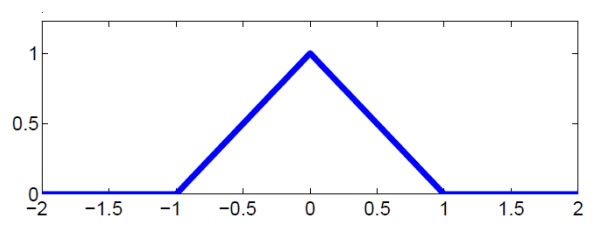
\includegraphics[width=0.5\textwidth]{MLbook/chapters/clustering/png/TSVMLoss.jpg}
    \caption{Вид функции штрафа для неразмеченных данных.}
    \end{figure}

\begin{figure}[ht]
    \centering
    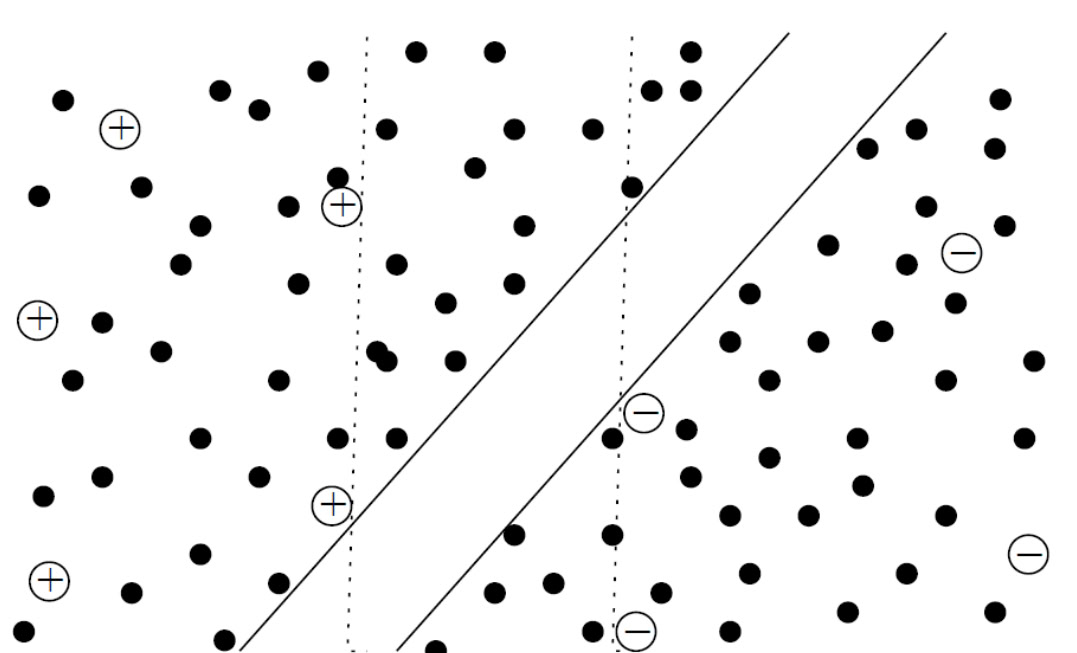
\includegraphics[width=0.5\textwidth]{MLbook/chapters/clustering/png/ClassifierData.jpg}
    \caption{Пример распределения точек около границы.}
\end{figure}

\subsection{Математическое описание трансдуктивной задачи}
С математической точки зрения новая трансдуктивная задача описывается следующим образом:

\begin{equation}
    Q(w, w_0) = \sum_{i=1}^{k} \left( 1 - \textcolor{red}{M_i(w, w_0)} \right)_+ + \frac{1}{2C} \|w\|^2 + \gamma \sum_{i=k+1}^{\ell} \left( 1 - |\textcolor{red}{M_i(w, w_0)}| \right)_+ \to \min_{\textcolor{red}{w, w_0}}.
\end{equation}

Данный подход позволяет учитывать как известные, так и неизвестные (неразмеченные) данные для более точного обучения модели.

\textbf{Основные преимущества и недостатки TSVM}:
\begin{itemize} 
    \item \textbf{Преимущества:} 
    \begin{itemize} 
        \item Как и в обычном SVM, можно использовать ядра для работы с нелинейными задачами. 
        \item Имеются эффективные реализации, которые позволяют работать с большими объемами данных. 
    \end{itemize}
        
    \item \textbf{Недостатки:}
    \begin{itemize}
        \item Задача оптимизации TSVM не является выпуклой, что делает методы оптимизации более сложными.
        \item Решение может быть неустойчивым, если нет области разреженности в данных.
        \item Требуется настройка двух параметров: \( C \) и \( \gamma \).
    \end{itemize}

    \item \textbf{Применение:} 
    TSVM используется в задачах, где важно учитывать как размеченные, так и неразмеченные данные для повышения точности классификации. Это делает метод особенно полезным для работы с большими объемами неразмеченных данных, которые часто встречаются в реальных приложениях.
\end{itemize}

\subsection{Задачи}
\subsubsection*{Номер 1}
\textbf{Условие:} Покажите на примере двух точек $(1/3, 1/3)$ и $(-2, -2)$ и линейного классификатора  с $w_0 = 0, w_1 = 1, w_2 = 1$ как именно считается модифицированная функция штрафа $L_U(M)$. \\
\textbf{Решение:}
Классифицирующей поверхностью в нашем случае является прямая $y = -x$ с соответствующей полосой, поэтому можем взять точки $(1/3, 1/3)$ и $(-2, -2)$ для того, чтобы продемонстрировать требуемое. Для них соответственно получаем:
\[
    L_1 = (1 - |(1/3*1 + 1/3*1 + 0)|)_+ = 1/3
\]

\[
    L_2 = (1 - |((-2)*1 + (-2)*1 + 0)|)_+ = 0
\]
\[
    L_{all} = 1/3 + 0 = 1/3
\]
Мы умножаем M на 1 вне зависимости от знака класса, т.к. в формуле стоит модуль, это опустили.
\subsubsection*{Номер 2}
\textbf{Условие:}
В рамках предыдущей задачи покажите, что для классификатора с теми же $w_1, w_2$, но $w_0 = -1$ получившийся штраф будет меньше. Соответствует ли это лучшей разделимости точек? Продемонстрируйте картинки с пояснениями.\\
\textbf{Решение:}
Аналогично будем иметь:
\[  
    L_1 = (1 - |(1/3*1 + 1/3*1 + 1)|)_+ = 0
\]

\[
    L_2 = (1 - |((-2)*1 + (-2)*1 + 1)|)_+ = 0
\]

\[
    L_{all} = 0 + 0 = 0
\]
Таким образом штраф уменьшился, и как видно из картинок, точки стали распределены вне линии разделения:
\begin{figure}[ht]
    \centering
    \begin{minipage}{0.45\textwidth}
        \centering
        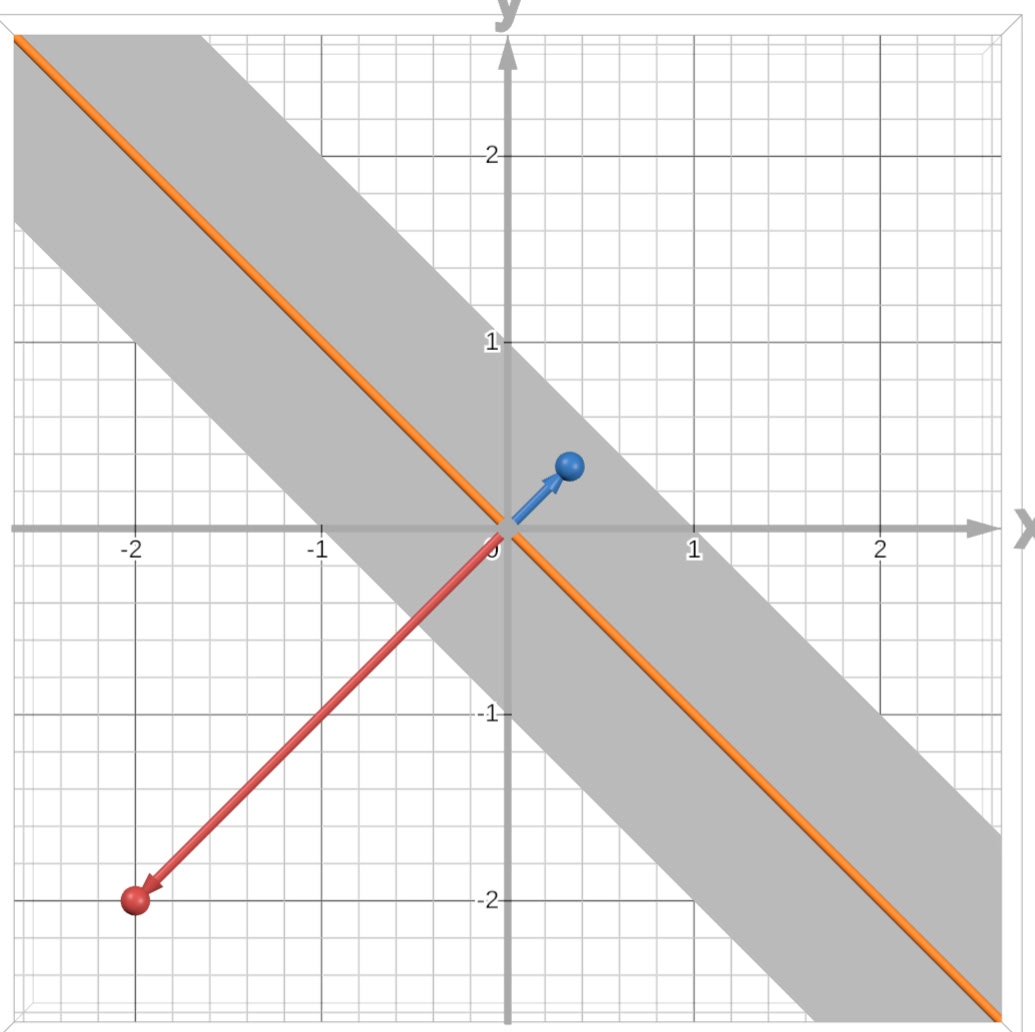
\includegraphics[width=0.9\textwidth]{MLbook/chapters/clustering/png/TSVM_3task1.jpg}
        \caption{$w_0 = 0$}
    \end{minipage}
    \hfill
    \begin{minipage}{0.45\textwidth}
        \centering
        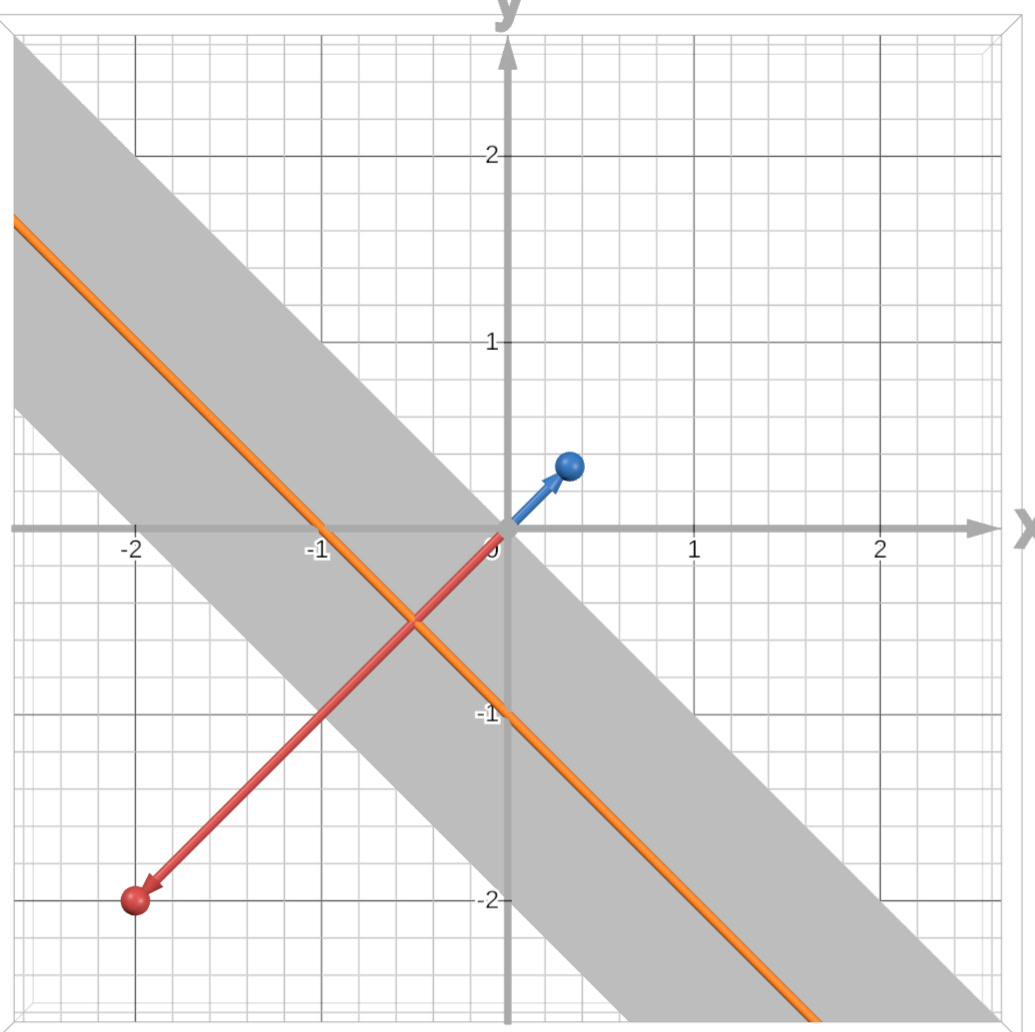
\includegraphics[width=0.9\textwidth]{MLbook/chapters/clustering/png/TSVM_3task2.jpg}
        \caption{$w_0 = -1$}
    \end{minipage}
\end{figure}

\subsubsection*{Номер 3}
\textbf{Условие:}
Можно ли использовать метод TSVM для постепенного самообучения, размечая данные по мере их поступления? Какие преимущества и недостатки могут быть у такого подхода?\\
\textbf{Решение:}\\
\textbf{Преимущества:}
\begin{itemize}
    \item \textbf{Эффективное использование неразмеченных данных:} Постепенное добавление размеченных данных на основе текущих предсказаний TSVM позволяет улучшить модель по мере поступления новых данных. Это может быть полезно, если размечать данные вручную дорого или занимает много времени.
    \item \textbf{Гибкость в обучении:} Метод TSVM может адаптироваться к новым данным и улучшать границу классификации, не требуя полного перерасчета модели с нуля каждый раз. Это особенно полезно в задачах, где данные поступают по мере времени (например, в потоках информации).
    \item \textbf{Обучение на малых объемах данных:} TSVM позволяет начать с небольшого набора размеченных данных и постепенно расширять его, используя информацию о неразмеченных примерах. Это важно, когда размеченные данные труднодоступны или ограничены.
\end{itemize}\\
\textbf{Недостатки:}
\begin{itemize}
    \item \textbf{Риски неправильной разметки:} Одной из проблем такого подхода является риск неверной или неточной разметки данных в процессе самообучения. Если начальная модель не обладает высокой точностью, ошибки в разметке могут привести к накоплению ошибок в дальнейшем обучении.
    \item \textbf{Проблемы с неопределенностью:} Неопределенные данные (примеры, которые находятся близко к границе принятия решения) могут быть ошибочно размечены. TSVM решает эту проблему через регуляризацию, но все же может столкнуться с трудностями при обработке сложных случаев, когда граница классификации неясна.
    \item \textbf{Зависимость от начальных данных:} Результат обучения сильно зависит от начального набора размеченных данных. Если эти данные не являются репрезентативными, то модель может в дальнейшем плохо обрабатывать новые примеры.
\end{itemize}


    \clearpage
    \chapter{Метод опорных векторов}
    \section{SVM-регрессия}
\subsection{Постановка задачи}
\par В задаче регрессии требуется найти функцию \( f(x) = w^T \phi(x) + b \), которая аппроксимирует целевые значения \( y \) на основе входных данных \( x \), минимизируя ошибки предсказания.
\par В SVM-регрессии вводится допустимая область погрешностей — \(\epsilon\)-окрестность. Это означает, что отклонения \( |f(x_i) - y_i| \) в пределах \(\epsilon\) считаются несущественными, и модель игнорирует их. Цель — минимизировать сложность модели, связанную с \(\|w\|\), штрафуя при этом за отклонения, выходящие за пределы \(\epsilon\).

\subsection{Прямая задача}
\par\textbf{Функция потерь.}  
Для задачи SVM-регрессии используется \(\epsilon\)-чувствительная функция потерь:
\begin{equation*}
    L_\epsilon(f(x), y) = 
    \begin{cases} 
        0, & \text{если } |f(x) - y| \leq \epsilon, \\ 
        |f(x) - y| - \epsilon, & \text{иначе.}
    \end{cases}
\end{equation*}
\noindent\textbf{Прямая постановка задачи:}
\begin{equation*}
    \min_{w, b} \frac{1}{2} \|w\|^2 + C \sum_{i=1}^n L_\epsilon(f(x_i), y_i),
\end{equation*}
где:
\begin{itemize}
    \item \(\|w\|^2\) — регуляризационный член, минимизирующий сложность модели,
    \item \(C\) — коэффициент, регулирующий баланс между штрафами за ошибки и сложностью модели,
    \item \(L_\epsilon(f(x_i), y_i)\) — штраф за выход за пределы \(\epsilon\)-окрестности.
\end{itemize}

\subsection{Преобразование задачи}
\par Для учёта отклонений выше \(\epsilon\) вводятся штрафные переменные \(\xi_i\) и \(\xi_i^*\):  
\begin{itemize}
    \item \(\xi_i\) — превышение сверху (\(y_i > f(x_i) + \epsilon\)),
    \item \(\xi_i^*\) — превышение снизу (\(y_i < f(x_i) - \epsilon\)).
\end{itemize}
\par Задача минимизации принимает вид:
\begin{equation*}
    \min_{w, b, \xi, \xi^*} \frac{1}{2} \|w\|^2 + C \sum_{i=1}^n (\xi_i + \xi_i^*),
\end{equation*}
при ограничениях:
\begin{equation*}
\begin{aligned}
    y_i - (w^T \phi(x_i) + b) \leq \epsilon + \xi_i, \\
    (w^T \phi(x_i) + b) - y_i \leq \epsilon + \xi_i^*, \\
    \xi_i, \xi_i^* \geq 0.
\end{aligned}
\end{equation*}

\subsection{Метод Лагранжа}
\par Для решения задачи вводится лагранжиан, который включает:
\begin{itemize}
    \item Целевую функцию,
    \item Ограничения через множители Лагранжа (\(\alpha, \alpha^*, \eta, \eta^*\)).
\end{itemize}
\par Лагранжиан записывается как:
\begin{equation*}
\begin{aligned}
    L(w, b, \xi, \xi^*, \alpha, \alpha^*, \eta, \eta^*) &= \frac{1}{2} \|w\|^2 + C \sum_{i=1}^n (\xi_i + \xi_i^*) - \\
    &\quad - \sum_{i=1}^n \alpha_i \big[ \epsilon + \xi_i - y_i + w^T \phi(x_i) + b \big] - \\
    &\quad - \sum_{i=1}^n \alpha_i^* \big[ \epsilon + \xi_i^* + y_i - w^T \phi(x_i) - b \big] - \\
    &\quad - \sum_{i=1}^n (\eta_i \xi_i + \eta_i^* \xi_i^*).
\end{aligned}
\end{equation*}
\par Для нахождения двойственной задачи необходимо минимизировать \(L\) по \(w\), \(b\), \(\xi\), \(\xi^*\) и максимизировать по множителям Лагранжа.

\subsection{Условия оптимальности}
\begin{enumerate}
    \item Производная по \(w\):
    \begin{equation*}
        \frac{\partial L}{\partial w} = w - \sum_{i=1}^n (\alpha_i - \alpha_i^*) \phi(x_i) = 0 \implies 
        w = \sum_{i=1}^n (\alpha_i - \alpha_i^*) \phi(x_i).
    \end{equation*}
    \item Производная по \(b\):
    \begin{equation*}
        \frac{\partial L}{\partial b} = \sum_{i=1}^n (\alpha_i - \alpha_i^*) = 0.
    \end{equation*}
    \item Производные по \(\xi_i\) и \(\xi_i^*\):
    \begin{equation*}
        \alpha_i + \eta_i = C, \quad \alpha_i^* + \eta_i^* = C, \quad 0 \leq \alpha_i, \alpha_i^* \leq C.
    \end{equation*}
\end{enumerate}

\subsection{Двойственная задача}
\par Подставляя условия оптимальности в лагранжиан, исключаем \(w\), \(b\), \(\xi_i\), \(\xi_i^*\). Получаем двойственную задачу:
\begin{equation*}
    \max_{\alpha, \alpha^*} -\frac{1}{2} \sum_{i,j=1}^n (\alpha_i - \alpha_i^*)(\alpha_j - \alpha_j^*) K(x_i, x_j) 
    - \epsilon \sum_{i=1}^n (\alpha_i + \alpha_i^*) + \sum_{i=1}^n y_i (\alpha_i - \alpha_i^*),
\end{equation*}
где \(K(x_i, x_j) = \phi(x_i)^T \phi(x_j)\) — ядровая функция.
\par Ограничения:
\begin{equation*}
    \sum_{i=1}^n (\alpha_i - \alpha_i^*) = 0, \quad 0 \leq \alpha_i, \alpha_i^* \leq C.
\end{equation*}
\par Для решения двойственной задачи используется метод квадратичного программирования.

\subsection{Построение финальной модели}
\par После решения двойственной задачи оптимальные \(\alpha_i\) и \(\alpha_i^*\) определяют параметры модели:
\begin{equation*}
    f(x) = \sum_{i=1}^n (\alpha_i - \alpha_i^*) K(x_i, x) + b.
\end{equation*}
\par Смещение \(b\) вычисляется через опорные векторы — точки, где выполняется одно из условий:
\begin{equation*}
    y_i - (w^T \phi(x_i) + b) = \epsilon, \quad \text{или} \quad y_i - (w^T \phi(x_i) + b) = -\epsilon.
\end{equation*}
\par Опорные векторы (\(\alpha_i > 0\) или \(\alpha_i^* > 0\)) определяют форму модели.

\subsection{Выбор ядра}
\par Выбор ядра играет ключевую роль в качестве работы модели SVM-регрессии. Различные ядра по-разному преобразуют входные данные, что может существенно повлиять на точность предсказаний и обобщающую способность модели.
\par Выбор ядра зависит от особенностей данных, структуры зависимости и доступных вычислительных ресурсов. Экспериментальная проверка нескольких типов ядер и последующая оценка метрик качества модели — это ключевой этап в процессе выбора оптимального ядра.
\par На рисунке ниже представлена SVM-регрессия с тремя типами ядер: RBF, линейным и полиномиальным. 
\begin{figure}[h!]
    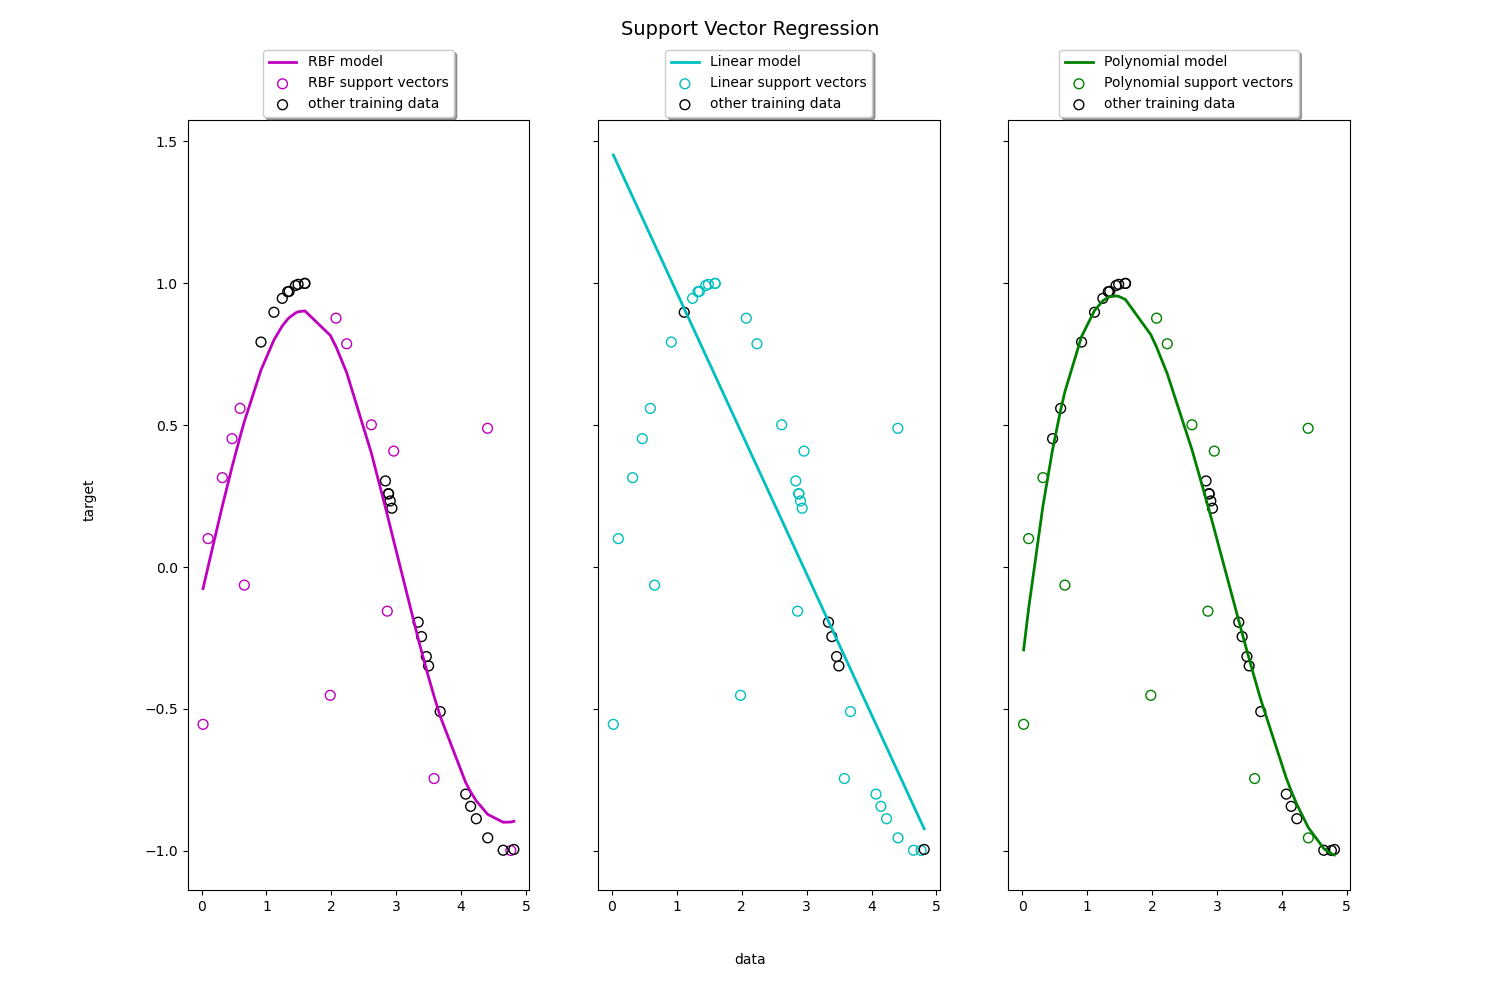
\includegraphics[width = 0.8\textwidth]{MLbook/chapters/svm/images/svm_regression_cmp_models.png}
    \centering
    \caption{Сравнение SVM-регрессия с разными типами ядер}
    \label{fig:kernel_comparison}
\end{figure}

\subsection{Задача 1}
\textbf{Условие}:
\par Рассмотрим следующий набор точек, лежащих на границе \(\epsilon\) - окрестности для SVM-регрессии с линейным ядром:
\begin{equation*}
    \{(1, 2), (2, 3), (3, 5), (4, 6)\}
\end{equation*}
\par Постройте регрессионную модель и найдите смещение \(b\), если \(w = 2\), \(\epsilon = 1\).
\par \noindent \textbf{Решение:}
\par Для нахождения смещения \(b\) необходимо использовать точки, которые лежат на границах \(\epsilon\)-окрестности. Мы знаем, что для таких точек выполняется равенство:
\begin{equation*}
    y_i - (w x_i + b) = \epsilon \quad \text{или} \quad y_i - (w x_i + b) = -\epsilon
\end{equation*}
\par Найдем для каждой точки \(b\), подставив их координаты в эти уравнения:
\begin{itemize}
\item Для точки \((1, 2)\):
\begin{equation*}
    2 - (2 \cdot 1 + b) = 1 \quad \Rightarrow \quad 2 - (2 + b) = 1 \quad \Rightarrow \quad -b = 1 \quad \Rightarrow \quad b = -1
\end{equation*}
\item Для точки \((2, 3)\):
\begin{equation*}
    3 - (2 \cdot 2 + b) = 1 \quad \Rightarrow \quad 3 - (4 + b) = 1 \quad \Rightarrow \quad -b = 2 \quad \Rightarrow \quad b = -2
\end{equation*}
\item Для точки \((3, 5)\):
\begin{equation*}
    5 - (2 \cdot 3 + b) = 1 \quad \Rightarrow \quad 5 - (6 + b) = 1 \quad \Rightarrow \quad -b = 2 \quad \Rightarrow \quad b = -2
\end{equation*}
\item Для точки \((4, 6)\):
\begin{equation*}
    6 - (2 \cdot 4 + b) = 1 \quad \Rightarrow \quad 6 - (8 + b) = 1 \quad \Rightarrow \quad -b = 3 \quad \Rightarrow \quad b = -3
\end{equation*}
\end{itemize}
\par Для вычисления окончательного значения смещения \(b\), усредняем найденные значения:
\begin{equation*}
    b_{\text{avg}} = \frac{-1 + (-2) + (-2) + (-3)}{4} = \frac{-8}{4} = -2
\end{equation*}
\par Таким образом, смещение \(b = -2\).
\par Регрессионная модель для SVM с линейным ядром имеет следующий вид:
\begin{equation*}
    f(x) = w x + b
\end{equation*}
\par Подставляем данное в условии значения \(w = 2\) и найденное значение \(b = -2\):
\begin{equation*}
    f(x) = 2x - 2
\end{equation*}
\par Это и есть наша линейная регрессионная модель.
\par \noindent \textbf{Ответ:} \(f(x) = 2x - 2\).

\subsection{Задача 2}
\textbf{Условие:}
\par У нас есть два набора данных для задачи регрессии:
\begin{itemize}
    \item Набор 1: \( \{(1, 2), (2, 3), (3, 4), (4, 5)\} \)    
    \item Набор 2: \( \{(1, 1), (2, 4), (3, 9), (4, 16)\} \)  
\end{itemize}
\par Предположим, что мы используем SVM-регрессию с различными типами ядер (линейное, полиномиальное, RBF). Определите, какое ядро будет оптимальным для каждого набора данных.
\par \noindent \textbf{Решение:}
\begin{itemize}
    \item Набор 1: данные имеют линейную зависимость, следовательно, линейное ядро будет лучшим выбором.

    \item Набор 2: данные имеют квадратичную зависимость, следовательно, оптимально будет использовать полиномиальное ядро второй степени.
\end{itemize}
\par \noindent \textbf{Ответ:} для первого набора данных оптимальным ядром будет линейное, для второго набора данных - полиномиальное второй степени.

\subsection{Задача 3}
\textbf{Условие:}
\par Дан набор данных для SVM-регрессии с линейным ядром: 
\begin{equation*}
    \{(1, 2), (2, 2.8), (3, 5.2), (4, 8)\}.
\end{equation*}
\par Параметры модели: \(w = 1.5\), \(b = 0.5\), \(\epsilon = 0.5\). 
\begin{enumerate}
    \item Определите, какие из точек набора данных находятся вне \(\epsilon\)-окрестности (требуют штрафных переменных \(\xi\) или \(\xi^*\)).
    \item Вычислите значения штрафных переменных для этих точек.
\end{enumerate}
\par \noindent \textbf{Решение:}
\begin{enumerate}
\item Определение границ \(\epsilon\)-окрестности:
   Уравнение модели SVM-регрессии с линейным ядром: 
   \begin{equation*}
    f(x) = wx + b.
   \end{equation*}
   Подсталяем данные в условии значения:
   \begin{equation*}
    f(x) = 1.5x + 0.5.
   \end{equation*}
   Границы \(\epsilon\)-окрестности:
   \begin{equation*}
    f(x) - \epsilon \leq y \leq f(x) + \epsilon.
   \end{equation*}
\item Проверка точек:
\begin{itemize}
    \item Для точки \((1, 2)\): 
    \begin{equation*}
        f(1) = 1.5 \cdot 1 + 0.5 = 2.0, \quad 2 - 0.5 \leq 2 \leq 2 + 0.5 \quad (\text{в окрестности}).
    \end{equation*}
    \item Для точки \((2, 2.8)\): 
    \begin{equation*}
        f(2) = 1.5 \cdot 2 + 0.5 = 3.5, \quad 3.5 - 0.5 \not\leq 2.8 \leq 3.5 + 0.5 \quad (\text{вне окрестности}).
    \end{equation*}
    \item Для точки \((3, 5.2)\): 
    \begin{equation*}
        f(3) = 1.5 \cdot 3 + 0.5 = 5.0, \quad 5.0 - 0.5 \leq 5.2 \leq 5.0 + 0.5 \quad (\text{в окрестности}).
    \end{equation*}
    \item Для точки \((4, 8)\): 
    \begin{equation*}
        f(4) = 1.5 \cdot 4 + 0.5 = 6.5, \quad 6.5 - 0.5 \leq 8.0 \not\leq 6.5 + 0.5 \quad (\text{вне окрестности}).
    \end{equation*}
\end{itemize}
\item Штрафные переменные:
\begin{itemize}
    \item Для точки \((2, 2.8)\):
    \begin{equation*}
        \xi_i = f(2) - y - \epsilon = 3.5 - 2.8 - 0.5 = 0.2.
    \end{equation*}
    \item Для точки \((4, 8)\):
    \begin{equation*}
        \xi_i^* = y - f(4) - \epsilon = 8 - 6.5 - 0.5 = 1.0.
    \end{equation*}
\end{itemize}
Таким образом, штрафные переменные:
\begin{equation*}
    \xi_2^* = 0.2, \quad \xi_4 = 1.0.
\end{equation*}
\end{enumerate}
\par \noindent \textbf{Ответ:} \(\xi_2^* = 0.2, \quad \xi_4 = 1.0.\)


\setcounter{secnumdepth}{0}

\section{1-norm SVM (LASSO SVM)}
\subsection*{Аппроксимация эмпирического риска с \(L_1\)-регуляризацией}
\begin{align*}
    \sum_{i=1}^{\ell} \left(1 - M_i(w, w_0)\right)_+ + \mu \sum_{j=1}^{n} |w_j| & \rightarrow \min_{w, w_0}
\end{align*}

\subsection*{Плюс: отбор признаков с параметром селективности \(\mu\)}
\begin{itemize}
    \item чем больше \(\mu\), тем меньше признаков останется
\end{itemize}

\subsection*{Минус: слишком агрессивный отбор признаков}
\begin{itemize}
    \item по мере увеличения \(\mu\) признак может быть отброшен, хотя $y$ существенно зависит от него (даже когда ещё не все шумовые признаки отброшены)
\end{itemize}

\newline
\newline

\section{Сравнение \(L_2\) и \(L_1\) регуляризации}

Зависимость весов \(w_j\) от коэффициента \(\frac{1}{\mu}\):

\begin{itemize}
    \item \(L_1\) регуляризатор: \(\mu \sum_{j} |w_j|\)
\end{itemize}

\begin{align*}
    \centering
    \includegraphics[width=0.6 \linewidth]{chapters/svm/images/L_1.png}
    \label{fig:image}    
\end{align*}

\begin{itemize}
    \item \(L_2\) регуляризатор: \(\mu \sum_{j} w_j^2\)
\end{itemize}

\begin{align*}
    \centering
    \includegraphics[width=0.6 \linewidth]{chapters/svm/images/L_2.png}
    \label{fig:image}    
\end{align*}

\section{Doubly Regularized SVM (Elastic Net SVM)}

\begin{align*}
    C \sum_{i=1}^{\ell} \left(1 - M_i(w, w_0)\right)_+ + \mu \sum_{j=1}^{n} |w_j| + \frac{1}{2} \sum_{j=1}^{n} w_j^2 & \rightarrow \min_{w, w_0}
\end{align*}

\subsection*{Плюсы:}
\begin{itemize}
    \item Параметр селективности \(\mu\) управляет отбором признаков: чем больше \(\mu\), тем меньше признаков останется
    \item Есть эффект группировки (grouping effect): значимые зависимые признаки отбираются вместе
\end{itemize}

\subsection*{Минусы:}
\begin{itemize}
    \item Шумовые признаки также группируются и могут вместе оставаться в модели
    \item Приходится подбирать два параметра регуляризации \(\mu, \tau\) (есть специальные методы, например, regularization path)
\end{itemize}

\subsection{Elastic Net Analysis}

Elastic Net менее жёстко отбирает признаки.

\begin{figure}[h]
    \centering
    \includegraphics[width=0.8\linewidth]{chapters/svm/images/Elastic_Net.png}
    \caption{Зависимости весов \(w_j\) от коэффициента \(\log \frac{1}{\mu}\)}
    \label{fig:mpr}
\end{figure}

\section{Support Features Machine (SFM)}

\begin{align*}
    C \sum_{i=1}^{\ell} \left(1 - M_i(w, w_0)\right)_+ + \sum_{j=1}^{n} R_{\mu}(w_{j}) & \rightarrow \min_{w, w_0}
\end{align*}

\begin{align*}
R_{\mu}(w_j)=
    \begin{cases}
        2\mu |w_j|, & |w_j| \leq \mu\\
        \mu^2 + w_j^2, & |w_j| \geq \mu \\
    \end{cases}
\end{align*}

\subsection*{Плюсы}
\begin{itemize}
    \item Только один параметр регуляризации \(\mu\)
    \item Отбор признаков с параметром селективности \(\mu\)
    \item Эффект группировки: значимые зависимые признаки ($|w_j|$ > \(\mu\)) входят в решение совместно (как в $Elastic$ $Net$)
    \item Шумовые признаки ($|w_j|$ < \(\mu\)) не группируются и подавляются независимо друг от друга (как в $LASSO$)
\end{itemize}

\section{Relevance Features Machine (RFM)}

\begin{align*}
    C \sum_{i=1}^{\ell} \left(1 - M_i(w, w_0)\right)_+ + \sum_{j=1}^{n} \ln(w_j^2 + \frac{1}{\mu}) & \rightarrow \min_{w, w_0}
\end{align*}

\begin{align*}
    R(w) = \ln(w^2 + \frac{1}{\mu}), \quad \mu = 0.1, 1, 100
\end{align*}

\subsection*{Плюсы}
\begin{itemize}
    \item Только один параметр регуляризации \(\mu\)
    \item Отбор признаков с параметром селективности \(\mu\)
    \item Есть эффект группировки
    \item Лучше отбирает набор значимых признаков, когда они только совместно обеспечивают хорошее решение
\end{itemize}

\section{Задачи}

\subsection{Задача 1}

Качественно объяснить, почему $L_1$-регуляризатор приводит к отбору признаков

\subsection{Ответ:}

Аппроксимация эмпирического риска с \(L_1\)-регуляризацией:
\begin{align*}
    \sum_{i=1}^{\ell} \left(1 - M_i(w, w_0)\right)_+ + \mu \sum_{j=1}^{n} |w_j| & \rightarrow \min_{w, w_0}
\end{align*}

\textcolor{red}{Почему \(L_1\)-регуляризатор приводит к отбору признаков?}

Замена переменных: 
\[
u_j = \frac{1}{2} (|w_j| + w_j), \quad v_j = \frac{1}{2} (|w_j| - w_j).
\]
Тогда 
\[
w_j = u_j - v_j \quad |w_j| = u_j + v_j.
\]

\begin{align*}
    \sum_{i=1}^{\ell} \left(1 - M_i(u - v, w_0)\right)_+ + \mu \sum_{j=1}^{n} (u_j + v_j) & \rightarrow \min_{u, v}, \\
    u_j \geq 0, \quad v_j \geq 0, \quad j = 1, \ldots, n.
\end{align*}

чем больше \(\mu\), тем больше индексов \(j\) таких, что \(u_j = v_j = 0\), но тогда \(w_j = 0\), значит, \textcolor{red}{признак не учитывается.}

\subsection{Задача 2}

Привести пример нежелательного эффекта в процессе обучения, с которым поможет справиться регуляризация 
 
\subsection{Ответ:}

Регуляризация помогает в случае линейной зависимости (мультиколлинеарности) признаков:\\
Пусть построен классификатор: $a(x, w) = sign\langle w, x \rangle$ \\
Мультиколлинеарность: $\exists$  $u \in \mathbb{R}^{n}$: $\forall x \in X$ $\langle u, x \rangle = 0$ \\
Неединственность решения и рост нормы вектора весов: $\forall \gamma \in \mathbb{R}$ $a(x, w) = sign\langle w, x \rangle = sign \langle w + \gamma u, x \rangle$ \\
\\
Проявления переобучения:
\begin{itemize}
    \item слишком большие веса $|w_j|$ разных знаков
    \item неустойчивость дискриминантной функции $\langle w, x \rangle$
    \item $Q(X^{\ell}) \ll Q(X^{k})$
\end{itemize}
Способ уменьшить переобучение:\\
регуляризация $||w|| \rightarrow min$ (сокращение весов, $weight$ $decay$)

\subsection{Задача 3}

Дана задача оптимизации:
\begin{align*}
    \frac{1}{2}(wx - b)^2 + \lambda|w| & \rightarrow \min_{w},
\end{align*}
где $x,$ $b$ $\in \mathbb{R};$ $\lambda \geq 0$\\
При каких $\lambda$ данная задачи имеет решение $w_0 \neq 0?$
 
\subsection{Ответ:}

Находим правую и левую односторонние производные в нуле и рассматриваем, когда они больше и меньше 0 соответственно:

\begin{align*}
    \begin{cases}
        -xb + \lambda > 0\\
        -xb - \lambda < 0\\
        \lambda \geq 0\\
    \end{cases} \Leftrightarrow \lambda > |xb|
\end{align*}

Это условие на $\lambda,$ при котором задача имеет решение $w_0 = 0,$ поэтому нам подходит $\lambda \in [0;$ $|xb|)$.


    \clearpage
    \chapter{Метод главных компонент}
    \section{Метод главных компонент}


Основной задачей метода главных компонент (он же PCA от Principal Component Analysis)  является минимизация ошибки восстановления данных, если они проецируются на подпространство меньшей размерности $k<d$, где $d$ - исходная размерность, а $k$ - уменьшенная. Функция потерь в этом случае задаётся как:

\[
L = \| \mathbf{X} - \mathbf{X}_{\text{proj}} \|_F^2,
\]

где:

\begin{itemize}
    \item \( \mathbf{X} \in \mathbb{R}^{n \times d} \) — исходная центрированная матрица данных, состоящая из $n$ векторов-строк из пространства размерности $d$;
    \item \( \mathbf{X}_{\text{proj}} = \mathbf{X} \mathbf{W} \mathbf{W}^\top \) — проекция данных на подпространство, заданное матрицей \( \mathbf{W} \);
    \item \( \| \cdot \|_F^2 \) — фробениусова норма, измеряющая суммарное отклонение всех точек данных от их проекций.
\end{itemize}

PCA минимизирует \( L \) путём выбора такого \( k \)-мерного подпространства, которое сохраняет максимальную часть дисперсии данных. \\

\textbf{Задача 1}. Докажите, что алгоритм последовательного построения главных компонент обладает свойством жадного отбора: локальные минимизации функции потерь путем добавления следующих главных компонент ведут к глобальной минимизации функции потерь для заданного числа главных компонент. 

\textit{Решение}
Действительно, алгоритм PCA заключается в следующем:\\

0. Если число главных компонент равно нулю, так, что мы проецируем данные на нульмерное пространство-точку, то оптимальной точкой будет начало координат, минимизирующее фробениусову норму

1. Выбираем первую главную компоненту (первый вектор базиса) так, чтобы выборочная дисперсия вдоль данной компоненты была минимальна. 

2. Вторую главную компоненту выбираем так, чтобы дисперсия данных вдоль нее была максимальна при условии ортогональности первой главной компоненте.

3. Аналогично выбираем третью главную компонету при условии ортогональности первой и второй. Далее действуем аналогично.


На каждом шаге будет получаться локально оптимальный выбор базиса главных компонент, при проекцировании данных на который функция потерь будет минимальна. Но поскольку каждый такой локальный базис является подбазисом объемлющего базиса и бОльшего числа главных компонент, который является глобально оптимальным, мы получаем, что локальные оптимизации функции потерь путем последовательного построения главных компонент приводят к глобально оптимальному базису.\\

\textbf{Задача 2}. Покажите, что $k$-ая главная компонента "важнее"  $k+1$ главной компоненты с точки зрения минимизации функции потерь.\\

\textit{Решение}. Это следует из вида функции потерь для $k$ главных компонент:

\[
\sum_{i=k+1}^d \lambda_i,
\]
где $\lambda_i$ - собственные числа ковариационной матрицы $\mathbf{\Sigma} = \frac{1}{n} \mathbf{X}^\top \mathbf{X}$, а также свойства собственных чисел: $ \lambda_{i+1} \leq \lambda_i$

\section{Автокодировщики в сравнении с PCA}

Автокодировщики представляют собой нейронные сети, предназначенные для обучения компактных представлений данных. Суть автокодировщика заключается в том, что он обучается на реконструкции исходных данных с помощью более компактной внутренней репрезентации (латентное пространство). В отличие от PCA, автокодировщики могут обучаться не только на линейных, но и на нелинейных зависимостях между признаками, что делает их более гибкими и мощными инструментами для снижения размерности.

Автокодировщик состоит из двух частей: энкодера и декодера. Энкодер преобразует исходные данные в скрытое представление (латентное пространство), а декодер восстанавливает исходные данные из этого представления. Обучение автокодировщика заключается в минимизации ошибки восстановления между исходными данными и их реконструкцией.

На лицо видна аналогия между PCA и автокодировщиками: 

1. Оба метода сжимают исходные данные: PCA в матрицу признаков меньшей размерности, а автокодировщик - в латентное пространство

2. Оба метода минимизируют фробениусову норму входной и выходной матриц: у PCA это матрица признаков, а у автокодировщиков, как правило, эта матрица (или тензор) представляет из себя изображение.

Однако у PCA есть полезные свойства, которыми не обладает обыкновенный автокодировщик: 

1. Главные компоненты отсортированы по обыванию их "важности" по минимизации функции потерь. Это позволяет жадным образом отбирать самые необходимые главные компоненты для сжатия данных.

2. Главные компоненты ортогональны и статистически независимы. Это повышает интерпретабельность PCA.



\section{Алгоритм PCAАE}

Оказывается можно построить автокодировщик, который обладает приведенными выше свойствами. Следуя авторам, будем называть его PCAAE (Principal Component Analysis Autoencoder) или PCA-автокодировщик.

Перед тем как описать PCA-автокодировщик, сначала определим некоторые обозначения. Пусть \( \mathbf{X} \) — это пространство данных, в общем случае мы будем рассматривать изображения размера \( n \times n \), то есть \( \mathbf{X} = \mathbb{R}^{n \times n} \). Обозначим латентное пространство как \( \mathbf{Z} = \mathbb{R}^d \), где \( d \) — размерность этого латентного пространства. Обозначим кодировщик как \( E: \mathbf{X} \to \mathbf{Z} \), а декодировщик как \( D: \mathbf{X} \to \mathbf{Z} \). Обозначим \( z_i \) как \( i \)-й компонент вектора \( \mathbf{z} \). Пусть \( y = D \circ E(\mathbf{x}) \) — это вывод автокодировщика. Кроме того, обозначим \( \mathbf{x}^{(i)} \) как \( i \)-й образец данных, а его код \( \mathbf{z}^{(i)} = E(\mathbf{x}^{(i)}) \). Наконец, будем обозначать \( i \)-ю версию кодировщика как \( E^{(i)}: \mathbf{X} \to \mathbb{R}^i \), и аналогично для декодировщика.

Теперь опишем основную идею и алгоритм PCA-автокодировщика. Как мы уже объяснили, есть два центральных вопроса, которые мы должны решить для определения PCA-автокодировщика:
\begin{itemize}
    \item Что мы понимаем под «увеличением важности» компонент латентного пространства, и как мы можем это наложить?
    \item Как мы можем обеспечить независимость латентных кодов?
\end{itemize}

В случае PCA важность определяется вариативностью данных вдоль оси, однако такое определение трудно применить к автокодировщику, так как в процессе обучения, как правило, все размерности латентного пространства заполняются. Таким образом, просто выполнить PCA на латентном пространстве не получится.

Поэтому мы вводим понятие важности, обучая серию автокодировщиков с увеличивающимся размером латентного пространства, начиная с латентного пространства размерности 1 (скаляр). В этом первом автокодировщике мы можем предположить, что информация наибольшей «важности» будет закодирована, в смысле минимизации потерь \( \ell_2 \). Например, это может быть средний цвет фона. Затем мы увеличиваем размер латентного пространства на 1, сохраняя ту же первую компоненту из предыдущего обучения: обучается только вторая компонента. Этот процесс повторяется итеративно, пока не будет достигнут предустановленный размер \( d_{\max} \). Заметим, что на каждой итерации предыдущий декодировщик отбрасывается, и новый обучается с нуля. Действительно, мы хотим наложить структуру на латентное пространство через обучение кодировщика, но декодировщик должен иметь возможность делать это по своему усмотрению.

Мы решаем второй вопрос, как наложить независимость на латентные коды, следующим образом. Для этого потребуем, чтобы величина ковариации каждой компоненты латентного пространства была как можно меньше. Мы можем достичь этого, добавив дополнительный член в функцию потерь автокодировщика, который будет учитывать эту зависимость. Предположим, что мы добавляем компоненту \( k \) в латентное пространство. Тогда для пакета данных размером \( M \), \( X = \{ \mathbf{x}^{(1)}, \dots, \mathbf{x}^{(M)} \} \), мы можем вычислить ковариацию по формуле:
\[
L_{\text{cov}}(X) = \sum_{i=1}^{k-1} \left[ \frac{1}{M} \sum_{j=1}^{M} \left( z_i^{(j)} z_k^{(j)} - \frac{1}{M} \sum_{j=1}^{M} z_i^{(j)} \sum_{j=1}^{M} z_k^{(j)} \right) \right].
\]

Чтобы упросить задачу, мы до латентного слоя применим batch normalisation, тогда получим: 

$$L_{\text{cov}}(X) = \frac{1}{M} \sum_{i=1}^{k-1} \sum_{j=1}^{M} z_i^{(j)} z_k^{(j)}
$$\\

\textbf{Задача 3}. Докажите утверждение выше.\\

\textit{Решение}.
Формула для batch normalisation имеет вид:
\[
y_i = \gamma \left( \frac{x_i - \mu}{\sqrt{\sigma^2 + \epsilon}} \right)
\]
Таким образом получается центрированный набор данных с нулевым средним, поэтому  $\sum_{j=1}^{M} z_i^{(j)} = 0$.\\

Итоговая функция потерь будет иметь вид:

$$L(X) = \frac{1}{M} \sum_{i=1}^{M} \left\| x^{(i)} - D \circ E(x^{(i)}) \right\|_2^2 + \lambda L_{\text{cov}}(X)
$$

Минимизируя эту функцию, мы, во-первых, добиваемся того, чтобы выходное изображение было похоже на входное, во-вторых, добиваемся как можно меньшей статистической зависимости между компонентами латентного пространства. 

\begin{thebibliography}{99}


\bibitem{article1} Saïd Ladjal, Alasdair Newson \textit{A PCA-Like Autoencoder}, arviv.org  2 Apr 2019.

\bibitem{article2} Saïd Ladjal, Alasdair Newson \textit{PCAAE: Principal Component Analysis Autoencoder for organising the latent space of generative networks}, arviv.org 14 Jun 2020.

\end{thebibliography}

\section{Введение в метод главных компонент(PCA)}
\textbf{Метод главных компонент (Principal Component Analysis, PCA)} — это статистический метод, используемый для снижения размерности данных с сохранением наиболее значимой информации. PCA находит новые признаки (главные компоненты), 
которые представляют собой линейные комбинации исходных признаков, причем эти компоненты ортогональны и ранжированы по величине объясняемой дисперсии.
\textbf{Основные этапы метода:} \\
1. \textbf{Центрирование данных}:\\ Данные центрируются так, чтобы среднее значение каждой переменной было равно нулю:
$$
X_c=X-\bar{X},
$$
где $X$ - исходная матрица данных (размер $n \times p$ ), $\bar{X}$ - вектор средних значений по столбцам.\\
2. \textbf{Построение ковариационной матрицы}: \\ Вычисляется ковариационная матрица:
$$
\Sigma=\frac{1}{n-1} X_c^T X_c
$$
где $\Sigma$ - симметричная матрица размером $p \times p$.\\
3. \textbf{Собственные значения и собственные векторы}: \\ Решается задача нахождения собственных значений и собственных векторов ковариационной матрицы:
$$
\Sigma \mathbf{v}_i=\lambda_i \mathbf{v}_i
$$
где $\lambda_i$ - собственные значения, $\mathbf{v}_i$ - соответствующие им собственные векторы.\\
4. \textbf{Ранжирование главных компонент}: \\ Собственные значения упорядочиваются по убыванию:
$$
\lambda_1 \geq \lambda_2 \geq \cdots \geq \lambda_p
$$
Первые несколько компонент, соответствующие самым большим собственным значениям, объясняют большую часть дисперсии данных.\\
5. \textbf{Проекция данных}: \\ Данные проецируются на главные компоненты:
$$
Z=X_c V_k,
$$
где $V_k$ — матрица $k$ собственных векторов, соответствующих $k$ наибольшим собственным значениям, $Z$ — матрица данных в пространстве главных компонент.

Свойства метода: \\
- Главные компоненты ортогональны:

$$
\mathbf{v}_i^T \mathbf{v}_j=0, \quad i \neq j
$$

- Дисперсия объясняется последовательностью собственных значений:

$$
\text { Объясненная дисперсия }=\frac{\sum_{i=1}^k \lambda_i}{\sum_{i=1}^p \lambda_i} \text {. }
$$

\section{Спектральный метод наименьших квадратов}

Ridge регрессия отделяет наименьшие собственные значения матрицы от нуля путем добаваления $\tau$ ко всем значениям. Аналогично PCA отделяет наименьшие собственные значения от 0, но другим методом, а именно просто не учитывает их(отбрасывает). Как будто в суммах вместо них просто стоят 0. Обобщение данного подхода и называется \textbf{Спектральным методом наименьших квадратов: } \\
Приведем алгоритм: 
\begin{enumerate}
    \item Строим SVD (Singular Value Decomposition) разложение, и упорядочиваем собственные значения по возрастанию: $\lambda_1 \geq \lambda_2 \geq \dots \geq \lambda_n$
    \item Есил среди них есть близкие к нулю значения(то есть у нас будет плохая обусловленность нашей матрицы $\Rightarrow$ мультиколлинеарность при обучении), то нам нужно найти способ отделения от 0 этих собственных значений: $\lambda_j \rightarrow \lambda^{'}_j \ \forall j = \overline{m,n}$. При этом собственные векторы не меняем. \\
    Рассмотим частные случаи:
    \begin{itemize}
        \item $\lambda^{'}_j = \lambda_j + \tau$ - гребневая регрессия (ridge regression)
        \item $\lambda^{'}_j = \lambda_j + I_{[j > m]}\infty$ - метод главных компонент (PCA)      
    \end{itemize}

    \item Применим формулы SVD для модификации МНК-решения: \\
     $$\alpha^{*} = \sum_{j =1}^{n} \frac{1}{\sqrt{\lambda_j}} u_j(v_j^Ty)  \rightarrow \alpha^{*} = \sum_{j =1}^{n} \frac{\sqrt{\lambda_j}}{\lambda^{'}_j} u_j(v_j^Ty)$$
     
     $$F\alpha^{*} = \sum_{j =1}^{n} v_j(v_j^Ty) \rightarrow F\alpha^{*} = \sum_{j =1}^{n} \frac{\lambda_j}{\lambda^{'}_j} v_j(v_j^Ty)
     $$
\end{enumerate}
Интуиция данного метода заключается в том, что мы вводим поправки для близких к нулю собсвенных значений ($\delta_j$) уменьшая вклад этих самых собственных значений. Эти паправки мы вольны варировать практически как угодно от небольших сдвигов (Ridge regression) и вплоть до $\infty$ (PCA).

\section{Задача низкорангового матричного разложения}
Сам метод PCA позволяет:
\begin{itemize}
    \item понижать размерность в задачах регресси/классификации
    \item генерировать новые признаки 
    \item формировать сжатое представление данных
\end{itemize}
Но это все задачи \textbf{низкорангового матричного представления}. \\
В общем случая задача следующая: \\
\textbf{Дано:} Матрица $Z = ||z_{ij}||_{n*m}, (i, j) \in \Omega \subset \{1, \dots, n\}*\{1, \dots, m\}$  \\ 
\textbf{Найти:} матрицы $X=||x_{it}||_{n*k}$ и $Y = ||y_{tj}||_{k*m}$ такие, что:  
$$
||Z-XY||^{2} = \sum_{(i,j) \in \Omega} (z_{ij} - \sum_t x_{it}*y_{tj})^2 \rightarrow \min_{X, Y}
$$
Из за дополнительных ограничений, мы вынуждены откзаться от SVD:
\begin{itemize}
    \item не квадратичная функция потерь
    \item неотрицательное матричное разложение $x_{it} \geq 0$, $y_{tj} \geq 0$
    \item разряженные данные: $|\Omega| \ll nm$
\end{itemize}

\section{Задачи на использование метода главных компонент}

\subsection{Задача 1: Вклад признаков в главные компоненты}
Пусть $X \in R_{n\times p}$ набор данных с n образцами (строками) и p признаками (столбцами). PCA стремится найти набор собственных векторов (главных компонент), которые максимизируют дисперсию данных при проецировании на эти векторы.

Задача состоит в том, чтобы математически оценить, какой вклад вносит каждый признак в главные компоненты, и проранжировать признаки в зависимости от их вклада.\\ \\
\textbf{Решение:}
Метод РСА ищет собственные векторы $\mathbf{v}_i$ и собственные значения $\lambda_i$ удовлетворяющие:

$$
\Sigma \mathbf{v}_i=\lambda_i \mathbf{v}_i,
$$


где $\lambda_i$ - величина дисперсии данных вдоль $\mathbf{v}_i$.
Собственные векторы $\mathbf{v}_i$ формируют матрицу $V=\left[\mathbf{v}_1, \mathbf{v}_2, \ldots, \mathbf{v}_p\right]$, где каждый столбец $\mathbf{v}_i$ указывает направления главных компонент.\\
\textbf{Вклад признака в главные компоненты:}\\

Каждый признак в $X$ вносит вклад в главные компоненты через веса собственных векторов $\mathbf{v}_i$ . Элементы $v_{i j}$ (где $v_{i j}-j$-й элемент $i$-го собственного вектора) определяют значимость $j$-го признака для $i$-й главной компоненты.

Вклад $j$-го признака в $i$-ю главную компоненту оценивается как квадрат соответствующего элемента $v_{i j}^2$ .\\

Общий вклад $j$-го признака во все главные компоненты можно найти, суммируя его взвешенные вклады с учётом дисперсий ( $\lambda_i$ ):\\
$j=\sum_{i=1}^p \lambda_i v_{i j}^2$.\\
Этот показатель учитывает как значимость признака для каждой компоненты $\left(v_{i j}^2\right)$, так и долю дисперсии, объясняемую компонентой ( $\lambda_i$ ).\\
На конкретном примере:
Пусть собственные вектора образуют матрицу V:

$$
V=\left[\begin{array}{cccc}
0.5 & 0.6 & 0.3 & 0.1 \\
0.4 & -0.7 & 0.2 & 0.5 \\
-0.6 & 0.2 & 0.7 & -0.4 \\
0.5 & 0.3 & -0.6 & -0.6
\end{array}\right]
$$
Собственные значения:

$$
\Lambda=\operatorname{diag}(4.0,2.5,1.2,0.3)
$$

Посчитаем вклад признака $1(j=1)$ :
Для этого берём первую строчку $V$ :

$$
v_{1, \cdot}=[0.5,0.6,0.3,0.1]
$$
Считаем:

$$
\begin{aligned}
\text { Contribution }_1 & =\left(0.5^2 \cdot 4.0\right)+\left(0.6^2 \cdot 2.5\right)+\left(0.3^2 \cdot 1.2\right)+\left(0.1^2 \cdot 0.3\right) \\
& =1.0+0.9+0.108+0.003=2.011
\end{aligned}
$$

То же самое повторяем для остальных строк и находим максимальное значение.
\subsection{Задача 2: Ошибка "реконструкции" PCA}
Пусть $X \in R_{n\times p}$ набор данных с $n$ образцами (строками) и $p$ признаками (столбцами), с помощью метода главных компонент нужно:
\begin{itemize}
\item{Спроецируйте данные в более низкоразмерное пространство, определяемое $k$ главными компонентами.}
\item {Реконструируйте исходные данные из пространства пониженной размерности.}
\item {Вычислите ошибку реконструкции и оцените, как она меняется в зависимости от количества сохраняемых компонент k.}
\end{itemize}
\textbf{Решение:}
Для реконструкции данных из $k$-мерного подпространства используется обратная проекция:

$$
\hat{X}=Z V_k^T+\bar{X}
$$


Здесь:
- $Z V_k^T$ возвращает проекцию данных в исходное $p$-мерное пространство.\\
- Добавление $\bar{X}$ восстанавливает исходное смещение данных. \\
Ошибка реконструкции должна показывать какую часть информации мы потеряли при использовании только $k$ компонент при репрезентации данных.\\
1. Определим ошибку реконструкции для одного объекта $x_i$ :

$$
E_i=\left\|x_i-\hat{x}_i\right\|^2=\left\|\left(x_i-\bar{X}\right)-\left(z_i V_k^{\top}\right)\right\|^2
$$

2. Обобщим на весь набор данных:

$$
E=\frac{1}{n \times p} \sum_{i=1}^n\left\|x_i-\hat{x}_i\right\|^2
$$

3. Заменим на выражение для $\hat{x}_i$:

$$
E=\frac{1}{n \times p} \sum_{i=1}^n\left\|x_i-\bar{X}-Z V_k^{\top}\right\|^2
$$
Мы получили выражение для ошибки реконструкции. Теперь докажем, что 
ошибка реконструкции $E$ уменьшается монотонно с $k$, и когда $k=p, E=0$.

1. Общая дисперсия данных - это след ковариационной матрицы, которая представляет собой сумму всех собственных значений:

$$
\text { Total Variance }=\sum_{j=1}^p \lambda_j
$$

2. Дисперсия, которую уловили $k$ компонент это:

$$
\text { Captured Variance }=\sum_{j=1}^k \lambda_j
$$

3. Ошибка реконструкции по сути является дисперсией, которую не удалось уловить, то есть просто:

$$
E=\text { Total Variance }- \text { Captured Variance }=\sum_{j=k+1}^p \lambda_j
$$

4. Так как $\lambda_1 \geq \lambda_2 \geq \cdots \geq \lambda_p \geq 0$, добавление большего числа компонент ( $k \rightarrow k+1$ ) уменьшает $E$ :

$$
\sum_{j=k+1}^p \lambda_j>\sum_{j=k+2}^p \lambda_j
$$

5. В тот момент, когда $k=p, \sum_{j=k+1}^p \lambda_j=0$ $\Rightarrow$ $E=0$.

\subsection{Задача 3: Построить критерий D-оптимальности для выбора лучших k-компонент }
Набор данных представляет собой матрицу $n \times p$, где n - число образцов (строк), а p - число признаков (столбцов). Введём критерий D-оптимальности, используемый для выбора подмножества точек из набора данных, которое максимизирует детерминант информационной матрицы.
$$
D_{opt} : max  det(X^{T}X)
$$

Ключевым свойством критерия D-оптимальности является то, что он максимизирует объём многомерной фигуры, которая получается из рассматриваемых признаков. \\
Нужно построить критерий D-оптимальности для выбора лучших 
k главных компонент, которые максимизируют детерминант объясненной дисперсии (или объём фигуры) в k-мерном подпространстве PCA. 

\textbf{Решение:}

Критерий D-оптимальности для подпространства $k$ задаётся максимизацией детерминанта информационной матрицы $\Lambda_k$ :

$$
D_{o p t}(k)=\max \operatorname{det}\left(\Lambda_k\right)
$$

Так как $\Lambda_k$ является диагональной матрицей, её детерминант равен произведению собственных значений:

$$
\operatorname{det}\left(\Lambda_k\right)=\prod_{i=1}^k \lambda_i
$$

Итак, наша задача сводится к выбору $k$-мерного подпространства (т.е. первых $k$ главных компонент), которые максимизируют произведение $\lambda_1 \cdot \lambda_2 \cdots \cdot \lambda_k$, что эквивалентно решению следующей задачи:

$$
\max _{V_k} \prod_{i=1}^k \lambda_i
$$


где $\lambda_i$ - собственные значения матрицы ковариации $\Sigma$.
Для вычисления $D_{\text {opt }}(k)$ :\\
\\
1. Центрируем данные:

$$
X_c=X-\bar{X},
$$


где $\bar{X}$ - матрица средних значений.\\
2. Вычисляем ковариационную матрицу:

$$
\Sigma=\frac{1}{n-1} X_c^T X_c
$$

3. Находим собственные значения $\lambda_1, \lambda_2, \ldots, \lambda_p$ и соответствующие собственные векторы $\mathbf{v}_1, \mathbf{v}_2, \ldots, \mathbf{v}_p$.\\
4. Выбираем первые $k$ собственных значений $\lambda_1, \lambda_2, \ldots, \lambda_k$, которые максимизируют:

$$
\prod_{i=1}^k \lambda_i
$$

Максимизация $\prod_{i=1}^k \lambda_i$ эквивалентна максимизации объёма \textbf{$k$-мерного эллипсоида}, описывающего данные в пространстве первых $k$ главных компонент. Это позволяет отобрать $k$ измерений, которые сохраняют максимальную дисперсию данных.


\section{Денойзинг данных с помощью метода главных компонент}
Метод главных компонент (PCA) — это один из самых распространенных и эффективных методов для снижения размерности данных, который также может быть применен для денойзинга. Денойзинг данных — это процесс удаления шума из наблюдений для выделения более чистых и значимых сигналов. Во многих областях, таких как обработка изображений, анализ звука, необходимо избавляться от шумов, которые могут искажать результаты анализа и ухудшать качество моделей.

Благодаря своей способности выявлять скрытые структуры в многомерных данных PCA может быть использован для денойзинга. При анализе данных PCA проецирует данные в пространство главных компонент. 

Основные моменты применения PCA для денойзинга включают:
\begin{itemize}
\item Выделение главных компонент: 
PCA позволяет выделить компоненты, вдоль которых данные наиболее рассеяны.

\item Реконструкция данных: Уменьшение уровня шума и восстановление более "чистого" сигнала могут быть произведены с помощью удаления компонент, у которых меньше дисперсия. 

\item Снижение размерности: PCA снижает размерность данных, что делает их более вычислительно эффективными. Это особенно полезно в контексте обработки больших объемов данных.
\end{itemize}

PCA выбирают по следующим причинам:
\begin{itemize}
\item Линейность: PCA представляет собой линейный метод, что делает его простым для интерпретации и анализа. Однако основной недостаток заключается в том, что он может не эффективно обрабатывать данные с нелинейными взаимосвязями.

\item Простота реализации: PCA является относительно простым в реализации. Многие библиотеки для анализа данных, такие как scikit-learn в Python, имеют встроенные инструменты для выполнения PCA.

\item Характеристики контекста: PCA позволяет не только проводить денойзинг, но и выявлять основные характеристики и структуры в данных, что часто полезно при анализе образцов.
\end{itemize}

PCA может значительно упростить сложные многомерные наборы данных, обеспечивая при этом сохранение наиболее важной информации. При этом снижение размерности данных может помочь в построении более легких и интерпретируемых моделей, что особенно важно в машинном обучении.
Однако у PCA есть и минусы. Так, отбрасывание компонент может привести к потере важной информации, если не удается точно оценить, какие компоненты следует сохранять. Ограниченность линейности также может быть недостатком, так как в данных со сложными и нелинейными зависимостями PCA может не обнаружить все важные структуры. Хотя PCA упрощает данные, интерпретировать полученные главные компоненты может быть непросто, поскольку они являются линейными комбинациями исходных переменных.

Таким образом, метод главных компонент является мощным инструментом для денойзинга данных, особенно в контексте многомерных наборов данных. Его способность выявлять значимую информацию и удалять шум делает его предпочтительным выбором в различных областях. Однако важно учитывать плюсы и минусы метода, чтобы правильно применять его в соответствии с конкретными задачами и свойствами данных. Выбор подходящего количества компонент и тщательная интерпретация результатов остаются ключевыми шагами, которые могут существенно повлиять на успех применения PCA для денойзинга.

\section{Задачи про денойзинг данных}
\textbf{Задача 1}\\
Пусть \( I \) — это набор изображений, состоящий из \( n \) изображений, каждое из которых имеет \( m \) пикселей. Изображения могут содержать шум, например, из-за помех во время съемки. Требуется устранить этот шум, сохраняя основные детали изображения с помощью PCA.

\underline{Решение:}
Данные можно представить в виде матрицы \( X \in \mathbb{R}^{n \times m} \), где строки соответствуют изображениям, а столбцы — пикселям. Далее необходимо центрировать данные, вычитая среднее значение по каждому столбцу (пикселю):
   \[
   X_{cen} = X - \mu
   \]
   где \( \mu \) — вектор среднего значения по всем изображениям.
Вычислим ковариационную матрицу:
   \[
   C = \frac{1}{n-1} X_{cen}^T X_{cen}
   \]
Далее необходимо найти собственные значения \( \lambda_i \) и собственные векторы \( v_i \) матрицы \( C \) и упорядочить собственные значения по убыванию. Отберем первые \( k \) собственных векторов, которые обеспечивают максимальную дисперсию, где \( k \) выбирается в зависимости от дисперсии. Запишем выбранные векторы в матрицу \( V_k \).
Спроектируем центрированные данные на выбранные главные компоненты:
   \[
   Z = X_{cen} V_k.
   \]
Реконструируем уменьшенную версию изображений, используя только \( k \) основных компонент:
   \[
   \hat{X} = Z V_k^T + \mu.
   \]

\textbf{Задача 2}\\
Пусть \( D \) --- оригинальные данные, которые содержат как полезную информацию, так и шум. После применения PCA к данным были получены очищенные данные (денойзинг) \( D' \). Оценить, насколько эффективно PCA справилось с устранением шума, используя метрику RMSE (Root Mean Square Error, RMSE).

\underline{Решение:}
Вычислим разницу (ошибку) между оригинальными и очищенными данными:
   \[
   E_{i} = D_{i} - D'_{i}, \quad \forall i = 1, 2, \ldots, n
   \]
Затем вычисляем RMSE для получения общих значений ошибок:
   \[
   RMSE = \sqrt{\frac{1}{n} \sum_{i=1}^{n} E_{i}^2} = \sqrt{\frac{1}{n} \sum_{i=1}^{n} (D_{i} - D'_{i})^2}
   \]

\textbf{Задача 3}\\
Пусть \( D \) --- оригинальные данные, которые содержат как полезную информацию, так и шум. После применения PCA к данным были получены очищенные данные (денойзинг) \( D' \). Оценить, насколько эффективно PCA справилось с устранением шума, используя коэффициент детерминации\( R^2 \).

\underline{Решение:}
   \[
   R^2 = 1 - \frac{\sum_{i=1}^{n} (D_{i} - D'_{i})^2}{\sum_{i=1}^{n} (D_{i} - \bar{D})^2}
   \]
   где \( \bar{D} \) — среднее значение оригинальных данных.

\end{document}

\section{Оценка оптимального числа главных компонент}
\subsection{Определение и идея метода}
PCA — это статистический метод, который позволяет сократить размерность данных, сохраняя при этом наибольшее количество информации. Главная идея PCA заключается в том, чтобы найти новые признаки, называемые главными компонентами, которые максимально коррелируют с исходными данными.\\

Математическое содержание метода главных компонент — это спектральное разложение ковариационной матрицы $\displaystyle C$, то есть представление пространства данных в виде суммы взаимно ортогональных собственных подпространств
$\displaystyle C$, а самой матрицы $\displaystyle C$ — в виде линейной комбинации ортогональных проекторов на эти подпространства с коэффициентами собственных значений $\displaystyle \lambda _{i}$. Если $X = \{x_{1}, ... ,x_{m}\}^{T}$  — матрица, составленная из векторов-строк центрированных данных, то $\displaystyle C =\frac {1}{m-1} X ^{T} X$

\\

\subsection{Почему важна оценка числа главных компонент?}
Оптимальное число главных компонент имеет большое значение, так как оно влияет на качество модели, интерпретацию результатов и общую эффективность анализа. Если число компонент слишком велико, это может привести к избыточности и переобучению, в то время как слишком малое число компонент может привести к потере важной информации.

\subsection{Сколько главных компонент необходимо?}

Не существует общепринятого объективного способа определить оптимальное число главных компонент. На самом деле, вопрос зависит от конкретной области применения и конкретного набора данных. Однако существуют подходы, которые могут служить руководством для ответа на этот вопрос.

\subsubsection{Метод объясненной дисперсии}
Этот метод заключается в выборе числа компонент так, чтобы доля объясненной дисперсии достигла заданного порога (например, 95\% или 99\%). Это позволяет сохранить большую часть информации при снижении размерности.

\subsubsection{Критерий Кайзера-Гуттмана}
Согласно правилу Кайзера, собственное значение главной компоненты больше 1 указывает на то, что компонента объясняет больше дисперсии, чем среднее значение одной переменной. Таким образом, компоненты с собственными значениями менее 1 не стоит сохранять, так как они приносят мало полезной информации. Иными словами значимы те главные компоненты, для которых $\displaystyle \lambda _{i}>\frac {1}{n} tr C$ то есть 
$\displaystyle \lambda _{i}$ превосходит среднее значение 
$ \displaystyle \lambda$ (среднюю выборочную дисперсию координат вектора данных). Правило Кайзера хорошо работает в простых случаях, когда есть несколько главных компонент с 
$\displaystyle \lambda _{i}$, намного превосходящими среднее значение, а остальные собственные числа меньше него. В более сложных случаях оно может давать слишком много значимых главных компонент. 

\subsubsection{Правило сломанной трости}
Набор нормированных на единичную сумму собственных чисел $(\displaystyle \lambda _{i}/ tr C, i = 1, ... ,n)$ сравнивается с распределением длин обломков трости единичной длины, ломанной в n − 1-й случайно выбранной точке (точки разлома выбираются независимо и равнораспределены по длине трости).

По правилу сломанной трости k-й собственный вектор (в порядке убывания собственных чисел $\lambda _{i}$ сохраняется в списке главных компонент, если $\frac {\lambda _{1}}{tr C} >l_{1}$

Говоря про визуальный анализ, этот метод часто упрощают до так называемого метода "локтя". Мы строим график, где по оси X отложено число компонент, а по оси Y - доля объясненной дисперсии. График будет иметь форму локтя, и точка, где снижение доли объясненной дисперсии замедляется, будет сильно приближенно указывать на оптимальное число компонент.

\subsection{Задачи}
\subsubsection*{Задача 1.}

У вас есть выборка из 50 объектов с 5 признаками, результаты анализа главных компонент: собственные значения 5.0, 2.0, 1.0, 0.5, 0.3. Какое минимальное количество компонент нужно выбрать, чтобы объяснить не менее 90\% дисперсии?

\begin{solution}
    Сумма собственных значений - 8.8. 90\% суммы = 7.92.
    
    5.0 + 2.0 = 7.0 (менее 90\%) - не достаточно

    5.0 + 2.0 + 1.0 = 8.0 (больше 90\%) - оптимальное число главных компонент 3 
\end{solution}
\subsubsection*{Задача 2.}

Предположим, что у нас есть 2 разных датасета с 4 признаками. Первый содержит информацию об жителях окраинного района типичного для страны N города. А именно уровне доходов, жилой площади, количестве топлива, покупаемого за месяц, и числе домашних животных на каждого жителя. Второй датасет - признаки, относящиеся к производительн работников какой-либо сферы: количество выходных часов, число сотрудников в группе, температура в помещении и время, провиденное за монитором. В каком из этих случаев вероятно ожидать, что оценка главных компонент будет нереалистичной и почему?  

\begin{solution}
    Скорее всего, в первом датасете при оценке главных компонент мы столкнемся с переоценкой их числа. Так как наши фичи достаточно схожие, все связаны с уровнем дохода, и, веротно, будет мультиколлинеарность в данных. Второе, так как это жители одного района какого-то типичного города возможно дисперсия каждой фичи будет низкой и значение каждого собственного числа будет низким.
\end{solution}


\section{Обозначения и постановка задачи}

\begin{itemize}
    \item $f_{1}(x), \dotsc, f_{n}(x)$ - старые признаки
    \item $g_{1}(x), \dots ,g_{m}(x)$ новые признаки, где $m<=n$ (размерность понижена)
    \item $\hat{f_j}$ - не сам старый признак, а его оценка, которая будет делаться по новым признакам
    \item Матрица "объекты-признаки" старая ($F$) и новая ($G$), у которой объекты те же, а вот признаки новые: \par
        $F_{l,n} = 
         \begin{pmatrix}
          f_1(x_1) &  \cdots & f_n(x_1) \\
          \vdots   &  \cdots & \vdots   \\
          f_1(x_l) &  \cdots & f_n(x_l) 
         \end{pmatrix}$ 
        $G_{l,m} = 
         \begin{pmatrix}
          g_1(x_1) &  \cdots & g_m(x_1) \\
          \vdots   &  \cdots & \vdots   \\
          g_1(x_l) &  \cdots & g_m(x_l) 
         \end{pmatrix}$
\end{itemize}

Требуем, чтобы старые признаки линейно восстанавливались по новым:\par
$\hat{f_j} = \displaystyle\sum_{s=1}^{m} g_s(x)u_{js}$, $\forall x \in X$\par Линейная комбинация новых признаков должна давать оценку старым признакам и эта оценка должна быть близка по всем элементам обучающей выборки: $x_1, \dotsc, x_l$

Мы хотим, чтобы по старым признакам восстанавливались новые с помощью линейного преобразования, таким образом, нам нужно найти матрицу этого преобразования. То есть нас интересует матричное произведение $GU^T$, где $G$ - матрица нового признакового описания. Все признаки умножения справа - это означает что мы имеем дело с линейной комбинацией признаков. Мы хотим, чтобы эти линейные комбинации давали нам матрицу $\hat{F}$ \approx $F$, то есть $\hat{F} = GU^T \approx F$ или же $GU^T$ должно быть как можно ближе к $F$ \par
 $U_{n,m} = 
 \begin{pmatrix}
  u_{1l} &  \cdots & u_{1m} \\
  \vdots &  \cdots & \vdots \\
  u_{nl} &  \cdots & u_{nm} 
 \end{pmatrix}$\par

 Данное условие можно записать в виде: \par
 $\displaystyle\sum_{i=1}^{l}\displaystyle\sum_{j=1}^{n} ((\hat{f_j}(x_i)-f_j(x_i))^2 = ||GU^T - F||^2$ \rightarrow min [$G$], [$U$]

То есть мы хотим представить матрицу $F_{lm}$ в виде двух матриц размера $l*n$ и $n*m$. Решим эту задачу. Можно заметить, что решение этой задачи записывается через сингулярное разложение. Более того, для метода главных компонент справедлива следующая теорема:\par


\section{Основная теорема метода главных компонент}

T: Основная теорема метода главных компонент\par
Если $m \le rk F$, где $F$ - исходная матрица, то минимум функционала $||GU^T - F||^2$ достигается, когда столбцы $U$ - это собственные векторы матрицы $F^TF$, соответствующие $m$ максимальным cобственным значениям $\lambda_1, \dotsc, \lambda_m$, а матрица $G = FU$. \par
При этом:
\begin{itemize}
    \item матрица $U$ ортонормирована: $U^TU = l_m$;
    \item матрица $G$ ортогональна: $G^TG = \Lambda = diag(\lambda_1,...,\lambda_m)$;
    \item $U\Lambda=F^TFU$; $G\Lambda=FF^TG$;
    \item $||GU^T-F||^2=||F||^2-tr\Lambda = \displaystyle\sum_{j=m+1}^n\lambda_j$
\end{itemize}

Весь метод называется методом главных компонент, потому что в нём максимальные  собственные значения и соответствующие им собственные векторы.\par
P.S. 3е свойство является просто записью того, что столбцы матрицы $U$ являются собственными векторами матрицы $F^T$. 

Эта теорема не просто связана с сингулярным разложением, а является более общим фактом и из неё можно получить сингулярное разложение как частный случай.

Сначала проговорим несколько замечаний, свойств данной теоремы:\par
Если взять $m=n$, то есть мы не занимаемся понижением размерности, то: \par
\begin{itemize}
    \item начение маленьких собственных значений просто 0, а значит $||GU^T - F||^2 = 0$
    \item представление $\hat{F}=GU^T=F$ точное и совпадает с сингулярным разложением при $G=\vee\sqrt{\Lambda}$:\par
    $F=GU^T=\vee\sqrt{\Lambda}U^T$; $U^TU=I_m$; $\vee^T\vee=I_m$
    \item линейное преобразование U работает в обе стороны: \par
    $F=GU^T$; $G=FU$ \par
\end{itemize}\par
Когда мы не теряем информацию, мы фактически только переходим к новому базису или к новым признакам, которые ортогональны. Поэтому такое преобразование называется декоррелирующим (или преобразованием Карунена-Лоэва).

    
Примеры применения данных свойств. Ортогональность признаков и диагональность G упрощает:
\begin{itemize}
    \item решение задачи вычисления псевдообратной матрицы
    \item построение МНК для линейной модели
    \item и др.
\end{itemize}

\section{Задачи}
\begin{enumerate}
    \item 
        Применение PCA к двумерным данным: \\
        Условие: Задан набор данных, состоящий из 5 точек в двумерном пространстве:  \\
         \begin{center}
         $X = 
             \begin{pmatrix}
              2 &  3 \\
              3 &  5 \\
              4 &  4 \\
              5 &  7 \\
              6 &  8 
             \end{pmatrix}$\par
        \end{center}
        Используя метод главных компонент, найдите главные компоненты для этого набора данных.
    \item 
        Снижение размерности: \\
        Условие: Задан набор данных с тремя признаками ($x1$, $x2$, $x3$) и десятью наблюдениями: \\
        \begin{center}
         $X = 
             \begin{pmatrix}
              x1 &  x2 &  x3\\
              1 &  2 &  3\\
              2 &  3 &  4\\
              3 &  4 &  5\\
              4 &  5 &  6\\
              5 &  6 &  7\\
              6 &  7 &  8\\
              7 &  8 &  9\\
              8 &  9 &  10\\
              9 &  10 &  11\\
              10 &  11 &  12\\
             \end{pmatrix}$\par
        \end{center}
        Используя метод главных компонент, уменьшите размерность данных до двух признаков.
    \item 
        Визуализация данных:
        Условие: Задан набор данных с четырьмя признаками \\
        ($x1$, $x2$, $x3$, $x4$) и восемью наблюдениями:
        \begin{center}
         $X = 
             \begin{pmatrix}
              x1 &  x2 &  x3 & x4\\
              1 &  2 &  1 & 3\\
              2 &  3 &  2 & 4\\
              3 &  4 &  3 & 5\\
              4 &  5 &  4 & 6\\
              5 &  6 &  5 & 7\\
              6 &  7 &  6 & 8\\
              7 &  8 &  7 & 9\\
              8 &  9 &  8 & 10\\
             \end{pmatrix}$\par
        \end{center}
        Используя метод главных компонент, визуализируйте данные в двумерном пространстве.
\end{enumerate}

\section{Решение задач}
\begin{enumerate}
    \item Шаги решения:\\
    \begin{itemize}
    \item Центрировать данные:\\
    (вычисляем среднее по каждому стоблцу):\\
    $x_{1-\text{mean}} = 4$;  $x_{2-\text{mean}} = 5.4$; 
    $mean = (x_{1-\text{mean}}, x_{2-\text{mean}})$    \\
    $X_{\text{centered}} = X - mean$
    \begin{center}
    $X_\text{centered} = 
             \begin{pmatrix}
              -2 &  -2.4 \\
              -1 &  -0.4 \\
              0 &  -1.04 \\
              1 &  1.6 \\
              2 &  2.6 
             \end{pmatrix}$\par
    \end{center}
    \item Вычислить ковариационную матрицу: \\
    $ C = \frac{1}{n-1} X_\text{centered}^T \cdot X_\text{centered}$
    \begin{center}
    $C = 
             \begin{pmatrix}
              2 &  3.2 \\
              3.2 &  4.8 \\
             \end{pmatrix}$\par
    \end{center}
    
   \item Найти собственные значения и собственные векторы: \\
   Решив характеристическое уравнение $ |C - \lambda I| = 0 $, получаем собственные значения $\lambda_1 = 6, \lambda_2 = 0.4$.\\  
   cобственные векторы соответствующие этим значениям:  \\
    $v_1 = (0.707, 0.707)$  и  $v_2 = (-0.707, 0.707)$.
   \item Выборать главной компоненты: \\  
   Первую главную компоненту можно взять как проекцию на  $v_1$.
   \end{itemize}
   
   \item Шаги решения:\\
   Аналогично первой задаче, предложим следующую последовательность шагов, для достидения решения: \\
   \begin{itemize} 
       \item Центрировать данные \\
        \begin{center}
        $X_\text{centered} = 
             \begin{pmatrix}
              -4.5 & -4.5 & -4.5 \\
              -3.5 & -3.5 & -3.5 \\
              -2.5 & -2.5 & -2.5 \\
              -1.5 & -1.5 & -1.5 \\
              -0.5 & -0.5 & -0.5 \\
              0.5 & 0.5 & 0.5    \\
              1.5 & 1.5 & 1.5    \\
              2.5 & 2.5 & 2.5    \\
              3.5 & 3.5 & 3.5    \\
              4.5 & 4.5 & 4.5
             \end{pmatrix}$\par
    \end{center}
    \item Вычислить ковариационную матрицу \\
       \begin{center}
        $C= 
             \begin{pmatrix}
              8.25 & 8.25 & 8.25    \\
              8.25 & 8.25 & 8.25    \\
              8.25 & 8.25 & 8.25
             \end{pmatrix}$\par
    \end{center}
    \item Найти собственные значения и векторы \\ 
       $\lambda_1 = 0, \lambda_2 = 24.75$.\\  
       cобственные векторы соответствующие $\lambda_1$:  \\
       $v_1 = (\frac{1}{\sqrt{3}}, \frac{1}{\sqrt{3}}, \frac{1}{\sqrt{3}})$ 
    \item Выборать главные компоненты: \\
        Выбираем первый собственный вектора и проецируем данные на него.
   \end{itemize}

   \item Шаги решения:\\\
   \begin{itemize} 
       \item Центрировать данные \\
       \item Вычислить ковариационную матрицу \\
       \item Найти собственные значения и векторы \\ 
       \item Выборать главные компоненты: \\
        Выбираем два первых собственных вектора и проецируем данные на них.
       \item Визуализировать данные: \\
       Для визуализации данных воспользуемся библиотекой matplotlib в python, все вышеперечисленные пункты решения так же можно выполнить с помощью python используя библиотеку numpy       
   \end{itemize}
\end{enumerate}

\section{Метод главных компонент  (Principal Component Analysis, PCA)}

\indent\textbf{Метод главных компонент  (Principal Component Analysis, PCA)} "--- метод обучения без учителя. Самодостаточный и не имеющий прямого отношения к методу многомерной линейной регрессии, хоть  может быть использован для решения регрессионных задач.

У нас есть исходные признаки $f_{1}(x), \dotsc, f_{n}(x)$, хотим их преобразовать таким образом, чтобы перейти в пространство пониженной размерности, то есть получить из $f$ такие новые признаки $g$, что $g_{1}(x)...g_{m}(x)$, где $m\leq$.

Получать новые признаки можно разными способами, но рассматриваем сейчас только линейное преобразование. Итак, требуем, чтобы старые признаки линейно восстанавливались по новым:\par
$\hat{f_j} = \displaystyle\sum_{s=1}^{m} g_s(x)u_{js}$, $\forall x \in X$, где $\hat{f_j}$ "--- не сам старый признак, а его оценка, которая будет делаться по новым признакам. \par Линейная комбинация новых признаков должна давать оценку старым признакам и эта оценка должна быть близка по всем элементам обучающей выборки $x_1, \dotsc, x_l$. То есть можно сформулировать критерий:\par

$\displaystyle\sum_{i=1}^{l}\displaystyle\sum_{j=1}^{n} ((\hat{f_j}(x_i)-f_j(x_i))^2 \rightarrow$ min [$g_s(x_i)$], [$u_{js}$] \par

Мы берём обучающую выборку $x_1, \dotsc, x_l$ и пользуемся МНК, чтобы построить такое преобразование, чтобы восстановленные признаки $\hat{f_j}$ были как можно ближе к исходным признакам $f_j$ по всем элементам обучающей выборки.\par Подразумевается, что новых признаков получится меньше, чем исходных, но по этим новым признакам исходные хорошо восстанавливаются. Фактически, мы хотим добиться сжатия информации. Таким образом можно заархивировать исходные вектора $f_j$. \textit{Если приводить аналогию с форматами сжатия изображений, то это jpeg - это тоже формат с потерей информации, но где объём теряемой информации это параметр, то есть мы можем управлять тем, насколько точно мы восстанавливаем исходную информацию по её сжатому представлению.} Значение функционала будет двойной суммы и будет давать погрешность восстановления, которую мы хотим минимизировать.

Перейдём к матричному обозначению. В матрицах строки "--- объекты, а столбцы "--- признаки. Матрица "объекты-признаки" старая ($F$) и новая ($G$), у которой объекты те же, а вот признаки новые: \par
$F_{l,n} =
 \begin{pmatrix}
  f_1(x_1) &  \cdots & f_n(x_1) \\
  \vdots   &  \cdots & \vdots   \\
  f_1(x_l) &  \cdots & f_n(x_l)
 \end{pmatrix}$
$G_{l,m} =
 \begin{pmatrix}
  g_1(x_1) &  \cdots & g_m(x_1) \\
  \vdots   &  \cdots & \vdots   \\
  g_1(x_l) &  \cdots & g_m(x_l)
 \end{pmatrix}$

Задача в том, чтобы по старым признакам восстанавливались новые с помощью линейного преобразования. То есть нас интересует матричное произведение $GU^T$, то есть $G$ - матрица нового признакового описания. Мы хотим, чтобы эти линейные комбинации признаков давали нам матрицу $\hat{F}$ \approx $F$, то есть $\hat{F} = GU^T$  \approx $F$ или же $GU^T$ должно быть как можно ближе к $F$ \par
 $U_{n,m} =
 \begin{pmatrix}
  u_{1l} &  \cdots & u_{1m} \\
  \vdots &  \cdots & \vdots \\
  u_{nl} &  \cdots & u_{nm}
 \end{pmatrix}$\par

 Данное условие можно записать в виде: \par
 $\displaystyle\sum_{i=1}^{l}\displaystyle\sum_{j=1}^{n} ((\hat{f_j}(x_i)-f_j(x_i))^2 = ||GU^T - F||^2$ \rightarrow min [$G$], [$U$]

Другой взгляд на задачу заключается в том, что это низкоранговое матричное разложение. То есть мы хотим матрицу $F_{lm}$ представить в виде двух матриц размера $l*n$ и $n*m$. Давайте решать эту задачу наиболее продуктивным способом. Рассмотрим поиск эффективной размерности выборки.

\section{Эффективная размерность выборки}
Обсудим как непсоредственно происходит понижение размерности и как определить нужную нам размерность $m$: \par

Берём собственные значения матрицы $F^TF$, упорядоченные по убыванию: \par
$\lambda_1 \geq \lambda_2 \geq \dotsc \geq \lambda_n \geq 0$ \par

Если задача обладает свойством мультиколлинеарности, то должно существовать пространство меньшей размерности, в котором реально находится почти вся выборка. То есть в пространстве $R^l$ $\exists$ некоторое многообразие меньшей размерности, в котором лежит выборка данных. Если это так, то в последовательности убывающих собственных значений можно будет увидеть картину "Критерия крутого склона": \par

\begin{figure}[h]
    \centering
    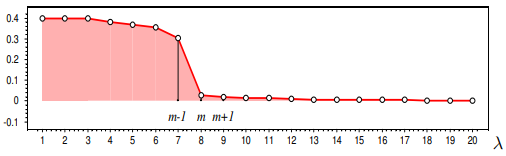
\includegraphics[width=1\linewidth]{Снимок экрана 2024-12-14 214833.png}
    \caption{Критерий крутого склона}
    \label{fig:enter-label}
\end{figure}

Математически можно записать, что эффективная размерность выборки - это наименьшее целое $m$, при котором: \par
$E_m = \frac{||GU^T-F||^2}{||F||^2} = \frac{\lambda_{m+1} + \dots + \lambda_{n}}{\lambda_{1} + \dots + \lambda_{n}} \leq \varepsilon$ \par

По этой картинке критерия крутого склона в моменте резкого падения можно найти $m$, после которого все значения будут близки к нулю. Это значит, что: $E_{m-1} \gg E_m$ и можно взять $m \leq n$ собственных значений и понизить размерность задачи. \par

А если крутого склона на графике нет? Если, например, у вас идёт монотонное, почти линейное снижение собственных значений до нуля это означает одно "--- никакой эффективной размерности у вас нет. Понизить размерность задачи линейными преобразованиями вам не удаётся и использовать МГК для такой задачи неприменим.

\section{Задачи на нахождение эффективной размерности выборки и их решение}
\begin{enumerate}
    \item \textbf{Задача про матрицу} \par
    Определить применим ли метод PCA для набора данных о 20 A  с 5ю характеристиками B, для которых матрица выглядит как:\par
     $\begin{pmatrix}
      4.4 &  0 & \cdots &  & 0 \\
      0  & 4.3 & 0 & \cdots &  0   \\
      0  & 0 & 4.2 & 0 & 0      \\
      0  & 0 & 0 & 4.1 & 0     \\
      0  & \cdots & \cdots & 0 & 4.0     \\
      0 & 0 & 0 & 0 & 0\\
      \vdots & \cdots & & \cdots &\vdots \\
      0 & 0 & 0 & 0 & 0\\
     \end{pmatrix}$ \par
     \textbf{Решение} \par
     \begin{itemize}
        \item найдём собственные значения и расположим их в убывающем порядке:\par
            \begin{itemize}
            \item $\lambda_{1}  = 4.0$
            \item $\lambda_{2}  = 4.1$
            \item $\lambda_{3}  = 4.2$
            \item $\lambda_{4}  = 4.3$
            \item $\lambda_{5}  = 4.4$
            \end{itemize}
        \item определим доли дисперсии по формуле $\frac{ \lambda_i }{\sum \lambda}$: \par
                \begin{itemize}
                \item $\frac{ \lambda_1 }{\sum \lambda}  = 0.1904$
                \item $\frac{ \lambda_2 }{\sum \lambda}  = 0.1952$
                \item $\frac{ \lambda_3 }{\sum \lambda}  = 0.2000$
                \item $\frac{ \lambda_4 }{\sum \lambda}  = 0.2048$
                \item $\frac{ \lambda_5 }{\sum \lambda}  = 0.2095$
            \end{itemize} \par
        \item построим график "крутого склона", где по оси OY откладывается значение долей дисперсии, а по оси OX "--- значение m. (Сам график опущен, мы уверены, что читатель справится построить его самостоятельно). \par
        \item по графику видно, что резкого падения или же крутого склона нет, а значит метод PCA для данных плохо применим.
     \end{itemize}\par
     \textbf{Ответ:} неприменим
    \item \textbf{Задача про анализы крови} \par
    Дан набор данных об анализах крови 15 пациентов с 5ю характеристиками (например, лейкоциты, эритроциты и тд), ковариационная матрица 15*5 представлена ниже. Определить применим ли метод PCA для этого набора данных и, если да, найти m "--- эффективную размерность выборки:\par    $\begin{pmatrix}
      2.1  & 1.8 & 1.2 & 0.9 & 0.7 \\
      1.9  & 1.6 & 1.1 & 0.8 & 0.6 \\
      1.8  & 1.5 & 1.0 & 0.7 & 0.5 \\
      1.7  & 1.4 & 0.9 & 0.6 & 0.4 \\
      1.6  & 1.3 & 0.8 & 0.5 & 0.3 \\
      1.5  & 1.2 & 0.7 & 0.4 & 0.2 \\
      1.4  & 1.1 & 0.6 & 0.3 & 0.1 \\
      1.3  & 1.0 & 0.5 & 0.2 & 0.1 \\
      1.2  & 0.9 & 0.4 & 0.1 & 0.1 \\
      1.1  & 0.8 & 0.3 & 0.1 & 0.1 \\
      1.0  & 0.7 & 0.2 & 0.1 & 0.1 \\
      0.9  & 0.6 & 0.2 & 0.1 & 0.1 \\
      0.8  & 0.5 & 0.2 & 0.1 & 0.1 \\
      0.7  & 0.4 & 0.2 & 0.1 & 0.1 \\
      0.6  & 0.3 & 0.2 & 0.1 & 0.1 \\
     \end{pmatrix}$ \par
     \textbf{Решение} \par
     \begin{itemize}
        \item найдём собственные значения и расположим их в убывающем порядке:\par
            \begin{itemize}
            \item $\lambda_{1}  = 5.2$
            \item $\lambda_{2}  = 3.1$
            \item $\lambda_{3}  = 0.8$
            \item $\lambda_{4}  = 0.5$
            \item $\lambda_{5}  = 0.4$
            \end{itemize}
        \item определим доли дисперсии по формуле $\frac{ \lambda_i }{\sum \lambda}$: \par
                \begin{itemize}
                \item $\frac{ \lambda_1 }{\sum \lambda}  = 0.52$
                \item $\frac{ \lambda_2 }{\sum \lambda}  = 0.31$
                \item $\frac{ \lambda_3 }{\sum \lambda}  = 0.08$
                \item $\frac{ \lambda_4 }{\sum \lambda}  = 0.05$
                \item $\frac{ \lambda_5 }{\sum \lambda}  = 0.04$
            \end{itemize} \par
        \item построим график "крутого склона", где по оси OY откладывается значение долей дисперсии, а по оси OX "--- значение m. (Сам график опущен, мы уверены, что читатель справится построить его самостоятельно). \par
        \item из графика видно, что есть резкий перегиб, то есть можно применить PCA
        \item Определим эффективные размерности, определяющие разные проценты выборки: \par
        \begin{itemize}
            \item 1 компонента даёт 52\%
            \item 2 компоненты дают 83\%
            \item 3 компоненты дают 91\%
            \item прибавление следующих компонент не внесёт серьёзный вклад
        \end{itemize}\par
        То есть для точности, например, в 80\% мы можем использовать размерность 2
    \end{itemize}
    \textbf{Ответ:} применим, для точности в 80\% достаточно размерности 2, а для точности 90\% "--- 3, дальнейшее повышение размерности (4 и полная размерность 5) не имеет смысла, так как усложняет вычисление задачи, но уточняет её несильно
    \item \textbf{Задача про машины} \par
    Дан набор данных о 1200 автомобилях с 14ю характеристиками (например: цвет, форма кузова, модель и др.), то есть матрица состоит из 1200 строк и 14 столбцов. Мы хотим использовать метод PCA для нахождения эффективной размерности выборки, чтобы, например, спрогнозировать цены на автомобили в зависимости от их характеристик. \par
    Шаги решения, которые мы предварительно применили:\par
    \begin{itemize}
        \item Отцентрировали данные, нашли средние значения характеристик
        \item Вычислили ковариационную матрицу
        \item Определили собственные значения и векторы. Собственные значения таковы: \par
        \begin{itemize}
            \item $\lambda_{1}  = 8.0$
            \item $\lambda_{2}  = 3.5$
            \item $\lambda_{3}  = 1.9$
            \item $\lambda_{4}  = 0.7$
            \item $\lambda_{5}  = 0.4$
            \item $\lambda_{6}  = 0.2$
            \item $\lambda_{7}  = 0.1$
            \item $\lambda_{8}  = 0.05$
            \item $\lambda_{9}  = 0.01$
            \item $\lambda_{10} = 0.005$
            \item $\lambda_{11} = 0.001$
            \item $\lambda_{12} = 0.0005$
            \item $\lambda_{13} = 0.0002$
            \item $\lambda_{14} = 0.0001$
        \end{itemize}
    \end{itemize}\par
    Доделайте задачу: \par
    \begin{itemize}
        \item Постройте график "крутого склона" и проведите анализ "сломанной трости"
        \item Найдите эффективную размерность, которая определяет 85\% общей дисперсии
    \end{itemize}\par
    \textbf{Решение} \par
    \begin{itemize}
        \item Предварительно нужно отсортировать по убывнию собственные значения $\lambda$. Проверили, на счастье, они уже расположены в нужном порядке. Теперь определим доли дисперсии по формуле $\frac{ \lambda_i }{\sum \lambda}$: \par
        \begin{itemize}
            \item $\frac{ \lambda_1 }{\sum \lambda}  = 0.538$
            \item $\frac{ \lambda_2 }{\sum \lambda}  = 0.235$
            \item $\frac{ \lambda_3 }{\sum \lambda}  = 0.127$
            \item $\frac{ \lambda_4 }{\sum \lambda}  = 0.047$
            \item $\frac{ \lambda_5 }{\sum \lambda}  = 0.027$
            \item $\frac{ \lambda_6 }{\sum \lambda} = 0.013$
            \item $\frac{ \lambda_7 }{\sum \lambda}  = 0.007$
            \item $\frac{ \lambda_8 }{\sum \lambda}  = 0.003$
            \item $\frac{ \lambda_9 }{\sum \lambda}  = 0.0006$
            \item $\frac{ \lambda_{10} }{\sum \lambda} = 0.0003$
            \item $\frac{ \lambda_{11} }{\sum \lambda} = 0.00006$
            \item $\frac{ \lambda_{12}}{\sum \lambda} = 0.00003$
            \item $\frac{ \lambda_{13} }{\sum \lambda} = 0.000013$
            \item $\frac{ \lambda_{14} }{\sum \lambda} = 0.000007$
        \end{itemize} \par
        По этим посчитанным данным строится график "крутого склона", где по оси OY откладывается значение долей дисперсии, а по оси OX "--- значение m. (Сам график опущен, мы уверены, что читатель справится построить его самостоятельно). \par
        Определяем точку перегиба, где всё стремится к нулю. Возле неё с заданной точностью будем определять эффективную размерность.
        \item Эффективная размерность, определяющая 85\% выборки соответсвует 3, так как: \par
        \begin{itemize}
            \item 1 компонента даёт 54\% (округлили 0,538 к доле 0,54 и записали в процентном соотношении)
            \item 2 компоненты дают 77\%
            \item 3 компоненты дают 90\%
        \end{itemize}\par
        \textbf{Ответ:} эффективная размерность "--- 3.
    \end{itemize}

\end{enumerate}

\section{Объясненная дисперсия после проекции. Проекция на пространство главных компонент, восстановление данных.}

\textbf{Метод главных компонент} (Principal Component Analysis, PCA) — это статистический метод преобразования пространства признаков, используемый для борьбы с мультаколлинеарностью в данных. В данном методе исходные признаки подвергаются некоторому функциональному преобразованию, при этом гарантируется линейная независимость новых признаков, и, возможное, сокращение их количества, то есть уменьшение размерности задачи. 

В методе главных компонент строится минимальное число новых признаков, по которым исходные признаки восстанавливаются линейным преобразованием с минимальными погрешностями. PCA относится к методам обучения без учителя (unsupervised learning), поскольку матрица «объекты–признаки» F преобразуется без учёта целевого вектора y.

Важно отметить, что PCA подходит и для регрессии, и для классификации, и для многих других типов задач анализа данных, как вспомогательное преобразование, позволяющее определить эффективную размерность исходных данных.

\textbf{Пусть}:

$f_1(x), ..., f_n(x)$ — исходные числовые признаки;

$g_1(x), ..., g_m(x)$ — новые числовые признаки, $m \leq n$;

\textbf{Требование}: старые признаки $f_i(x)$ должны линейно восстанавливаться по новым признакам $g_s(x)$:
\begin{equation}
    \hat{f}_j(x) = \sum_{i=1}^{m}g_s(x)u_{js}, \quad j = 1, ..., n, \quad \forall x \in X, 
\end{equation}
как можно точнее на обучающей выборке $x_1, ..., x_l$:
\begin{equation}
    \sum_{i=1}^{l}\sum_{j=1}^{n}(\hat{f}_j(x_i) - f_j(x_i))^{2} \rightarrow \underset{\{g_s(x_i)\}, \{u_{js}\}}{\min}
\end{equation}

Перейдем к матричным обозначениям. Матрицы объекты-признаки, старая и новая:
\begin{equation}
    \underset{l \times n}{F} = \begin{pmatrix} f_1(x_1) \quad ... \quad f_n(x_1) \\ ... \quad ... \quad ... \\ f_1(x_l) \quad ... \quad f_n(x_l) \end{pmatrix}; \quad \underset{l \times m}{G} = \begin{pmatrix} g_1(x_1) \quad ... \quad g_m(x_1) \\ ... \quad ... \quad ... \\ g_1(x_l) \quad ... \quad g_m(x_l) \end{pmatrix}.
\end{equation}
Матрица линейного преобразования новых признаков в старые:
\begin{equation}
    \underset{n \times m}{U} = \begin{pmatrix} u_{11} \quad ... \quad u_{1m} \\ ... \quad ... \quad ... \\ u_{n1} \quad ... \quad u_{nm} \end{pmatrix}; \quad \hat{F} = GU^{T} \approx F.
\end{equation}

\textbf{Цель}: найти и новые признаки G, и преобразование U по изветсной матрице F:
\begin{equation}
    \sum_{i=1}^{l}\sum_{j=1}^{n}(\hat{f}_j(x_i) - f_j(x_i))^{2} = \left\| GU^{T} - F \right\|^{2} \rightarrow \underset{G, U}{min},
\end{equation}

Решение помогает найти следующая теорема:

\textbf{Теорема}. Если $m \leq rk F$, то минимум $\left\| GU^{T} - F \right\|^{2}$ достигается, когда столбцы матрицы $U$ — это собственные векторы матрицы $F^{T}F$, соответствующие $m$ максимальным собственным значениям $\lambda_1, ..., \lambda_m$, а матрица $G = FU$.

При этом:

1. матрица $U$ ортонормирована: $U^{T}U = \hat{1}_m$;

2. матрица $G$ ортогональна: $G^{T}G = \Lambda = diag(\lambda_1, ..., \lambda_m)$;

3. $U \Lambda = F^{T}FU; G\Lambda = FF^{T}G$;

4. $\left\| GU^{T} - F \right\|^{2} = \left\|F\right\|^{2} - tr \Lambda = \sum_{j = m+1}^{n} \lambda_j$.

Таким образом, минимум функции $\left\| GU^{T} - F \right\|^{2}$ равен сумме наименьших собственных значений.

\textbf{Применение}: Сперва данные центрируются так, чтобы средние значения всех переменных были раны нулю, а именно:
\begin{equation}
    F_{centered} = F - \bar{F},
\end{equation}
где $F$ исходное признаковое описание данных, а $\bar{F}$ вектор средних значений по столбцам.

Далее происходит построение ковариационной матрицы:
\begin{equation}
    \Sigma = \frac{1}{n-1}F_{centered}^{T}F_{centered}.
\end{equation}

Следующий шаг — это найти собственные значения и собственные векторы ковариационной матрицы:
\begin{equation}
    \Sigma \mathbf{u_i} = \lambda_i \mathbf{u_i}.
\end{equation}
Впоследствии из них выбираются несколько главных компонент (собственных векторов), соответствующих наибольшим собственным значениям, объясняющих большую часть данных.

Последним шагом является проецирование исходных данных на главные компоненты:
\begin{equation}
    Z = F_{centered}U_k,
\end{equation}
где $U_k$ — матрица $k$ отобранных собственных вектров (главных компонент), Z — это матрица исходных данных, представленных в пространстве главных компонент.

\textbf{Объясненная дисперсия}. Для оценки меры того, насколько признаки в новом пространстве хорошо описывают исходные данные используется объясненная дисперсия. Объясненная дисперсия отражает долю общей дисперсии зависимой переменной, которая может быть объяснена независимыми переменными в модели. 
\begin{equation}
    \text{Объясненная дисперсия} = \frac{\sum_{i=1}^{k}\lambda_i}{\sum_{i=1}^{n}\lambda_i}.
\end{equation}

\textbf{Восстановление исходных данных}. Для восстановления исходных данных используется следующая формула:
\begin{equation}
    F_{reconstructed} = Z U_{k}^{T} + \bar{F}, 
\end{equation}
где Z — матрица проекций на главные компоненты.

При восстановлении данных всегда возникает ошибка, которая определяется как разница между исходными данными и восстановленными данными. Эта ошибка может быть измерена с помощью среднеквадратичной ошибки (MSE):
\begin{equation}
    MSE = \frac{1}{n} \sum_{i = 1}{l} \left\|F_i - F_{reconstructed, i} \right\|^{2},
\end{equation}
где l — количество наблюдений, $F_i$ — исходные данные, а $F_{reconstructed}$ — восстановленные данные.

\textbf{Задача 1.}

\textit{Условие}. Рассмотрим набор данных с тремя признаками $X_1, X_2, X_3$ с матрицей ковариации:
\begin{equation}
    \Sigma = \begin{pmatrix} 4 \quad 2 \quad 0 \\ 4 \quad 3 \quad 1 \\ 0 \quad 1 \quad 2 \end{pmatrix}.
\end{equation}
Найдите долю объясненной дисперсии, приходящейся на каждую лавную главную компоненту.

\textit{Решение}. Найдем собственные значения матрицы ковариации:
\begin{equation}
    det \begin{pmatrix} 4 - \lambda \quad 2 \quad 0 \\ 4 \quad 3 - \lambda \quad 1 \\ 0 \quad 1 \quad 2 - \lambda \end{pmatrix} = 0 \quad \rightarrow \quad \lambda_1 = 0, \lambda_2 = 2, \lambda_3 = 6.
\end{equation}
Найдем долю объясненной дисперсии, приходящейся на каждую лавную главную компоненту:
\begin{equation}
    \text{Доля}_1 = \frac{\lambda_1}{\lambda_1 + \lambda_2 + \lambda_3} = \frac{0}{0 + 2 + 6} = 0,
\end{equation}
\begin{equation}
    \text{Доля}_2 = \frac{\lambda_2}{\lambda_1 + \lambda_2 + \lambda_3} = \frac{2}{0 + 2 + 6} = 0.25,
\end{equation}
\begin{equation}
    \text{Доля}_3 = \frac{\lambda_3}{\lambda_1 + \lambda_2 + \lambda_3} = \frac{6}{0 + 2 + 6} = 0.75.
\end{equation}

\textbf{Задача 2.}

\textit{Условие}. Рассмотрим набор данных с двумя признаками $(X1, X2)$: $X_1 = (-1, -1, 2), X_2 = (2, -1, -1)$. Найдите проекцию данных на первую главную компоненту.

\textit{Решение}. 1. Центрирование данных. Средние значения: 
\begin{equation}
    \bar{X}_1 = \frac{-1 - 1 + 2}{3} = 0 \quad \bar{X}_2 = \frac{2 - 1 - 1}{3} = 0.
\end{equation}
Центрированные данные: 
\begin{equation}
    X_{centered} = \begin{pmatrix} -1 & 2 \\ -1 &  -1 \\ 2 & -1 \end{pmatrix}.
\end{equation}

2. Вычисление ковариационной матрицы. Ковариационная матрица $C$ вычисляется как:
\begin{equation}
    \Sigma = \frac{1}{n-1}X_{centered}^{T}X_{centered},
\end{equation}
где $n = 5$ - количество наблюдений.
После расчетов получаем:
\begin{equation}
    \Sigma = \begin{pmatrix} \text{Var}(X_1) & \text{Cov}(X_1, X_2) \\ \text{Cov}(X_1, X_2) & \text{Var}(X_2) \end{pmatrix} = \begin{pmatrix} 1.5 & -0.75 \\ -0.75 & 1.5 \end{pmatrix}
\end{equation}

3. Решая характеристическое уравнение $|\Sigma - \lambda \hat{1}| = 0$ находим собственные значения: $\lambda_1 = 0.75, \quad \lambda_2 = 2.25$.

Собственные векторы соответствующие этим собственным: $u_1 = (1, 1), \quad u_2 = (-1, 1)$.

4. Проекция на первую главную компоненту. Проекция данных на первую главную компоненту осуществляется следующим образом: $Z = X_{centered} v_1^T$. После вычислений получаем проекцию: $Z =\begin{pmatrix} 1 \\ -2 \\ 1 \end{pmatrix}$.

\textbf{Задача 3.}

\textit{Условие}. В задаче 2 восстановите исходные данные из полученной проекции.

\textit{Решение}. Для восстановления данных используем формулу: 
\begin{equation}
    X_{reconstructed} = Zu_1 + \bar{X},
\end{equation}
 где $\bar{X} = (0, 0)$.

 Тогда $X_{1, reconstructed} = (1, -2, 1), X_{1, reconstructed} = (-1, 2, -1)$.


\section{Анализ соответствий}
\textbf{Анализ соответствий (Correspondence analysis (CA)} — обобщение метода главных компонент, предназначенное для работы с
категориальными признаками. Другие имена, существующие из-за того, что технику CA часто переоткрвали -- "dual scaling,” “optimal scaling,” “homogeneity analysis” или “reciprocal averaging". CA отображает матрицу признаков в два множество новых переменных, которые называются "factor scores".\\
Factor scores  дают подобраны так, что они оптимальным образом отображают похожесть строк (первое множество) и столбцов (второе) изначальной таблицы. В двух множествах роль factor scores играют точки, чьи  измерения также называют \textit{компонентами}, что подчёркивает связь с PCA. Если быть точнее, factor scores отвечают за вклад каждой из ортогональных компонент в итоговую матрицу.\\
В силу нехватки места, будем детально рассматривать CA для 2х категориальных признаков.\\
Мы будем анализировать данные сразу по таблице сопряжённости, т.е. таблици типа 
\begin{table}[H]\centering
\begin{tabular}{|c|c|c|}
\hline  & Right-handed & Left-handed  \\
\hline Male & 43 & 9 \\
\hline Female & 44 & 4  \\
\hline
\end{tabular}
\end{table}
\subsection{Описание метода}
Для начала преобразуем таблицу в матрицу вероятностей. Для этого разделим все элементы матрицы на сумму матрицы и получим матрицу \textbf{Z}.\\
Пусть $r=Z\textbf{1}$, $c=Z^T\textbf{1}$. Затем пусть $D_c=\text{diag\{c\}}$, $D_r=\text{diag\{r\}}$.\\
Теперь рассмотрим матрицу $S=D_r^{-1/2}(Z-rc^T)D_c^{-1/2}$.
Разложим матрицу по SVD (сингулярное разложение)
$$S=P\Delta Q^T$$
Матрица P (соответственно Q) содержит левые
(соответственно правые) сингулярные векторы матрицы $S$. Диагональные элементы
диагональной матрицы $\Delta$ являются её сингулярными значениями. 
По свойствам SVD, аналогично PCA, квадраты сингулярных значений будут собственными значениями матрицы $S^TS$; пусть $\Lambda=\Delta^2$. Эти собственные значения, все так же, как в PCA, выражают дисперсию, соответствующим фактором, а их сумма называется общей инерцией изначальной матрицы.\\
Теперь factor scores получаются по следующей формуле:
$$F=D_r^{-1/2}P\Delta\text{ и }G=D_c^{-1/2}Q\Delta$$
(раньше, в PCA, была одна марица из $X=P\Delta Q^T$, равная $F'=P\Delta$, для неё $F'=P\Delta=XQ$; $X=F'Q^T$, т.е. ортогональная матрица $Q^T$ по сути то, куда мы проецируем).
\subsection{Что тут оптимального?}
Критерий, по которому CA оптимален -- дисперсия factor scores. Например, первая строка $f_1$ у матрицы $F$ -- линейная комбинация столбцов $Z-rc^T$, с ограничениями от $D_r^{-1/2}$, $D_c^{-1/2}$, точнее $$f_1=D^{-1}_r(Z-rc^T)D^{-1}_cq_1$$$$\textbf{s.t.} f_1=\arg\max\limits_{f}f^TD_rf$$$$ q_1^TD_c^{-1}q_1=1$$  
Не менее важное свойства CA -- то, что он оптимален \textit{с точки зрения $\chi^2$}. Точнее, общая инерция строк пропорционально $\chi^2$ из теста Пирсона для нуль-гипотезы того, что строки и столбцы независимы:
$$\chi^2=N\sum_i^I\sum_j^J\frac{(z_{ij}-r_ic_j)^2}{r_ic_j}=N\phi^2$$.\\
Как следует из курса статистики, при верности нуль-гипотезы этот притерий имеет распределение $\chi^2\left((I-1)(J-1)\right)$, и с его помощью можно проверять нуль-гипотезу.\\
Общая инерция матрицы $S$ вычисляется по следующей формуле:
$$\mathcal{I}=\text{tr}\left\{S^TS\right\}=\sum_i^I\sum_j^J\frac{(z_{ij}-r_ic_j)^2}{r_ic_j}=\phi^2$$
Таким образом, факторы СА выполняют ортогональное разложение критерия $\chi^2$, где каждый фактор "объясняет" часть отклонение от независимости строк.
Ещё одно свойство, то, что дисперсия factor scores для всех строк и столбцов одинакова. И вообще, можно получить F из G и G из F:
$$F=D_r^{-1/2}P\Delta=D_r^{-1/2}SQ=D_r^{-1}(Z-rc^T)D_c^{-1/2}Q=D_r^{-1}(Z-rc^T)G\Delta^{-1}=D_r^{-1}ZG\Delta^{-1}-D_r^{-1}rc^TG\Delta^{-1}$$
А затем, по построениею $r$ и $c$, вторая компонента равна 0, а значит
$$F=D_r^{-1}ZG\Delta^{-1}$$
Аналогично $$G=D_c^{-1}Z^TF\Delta^{-1}$$.
\section{Некоторые задачи на анализ соответствий}
\subsection{Задачи по анализу соответствий}
\problem Пусть $X\in\mathbb{R}_{nxp}$ -- таблица сопряженности. Понять, какую значимость имеет каждый признак. Даны следующие данные.
(Подсказка: нужно поситать пропорцию инерций, как в 1 задаче для PCA)

a) \begin{table}[H]\centering
\begin{tabular}{ccc}
\toprule
Right-handed & Left-handed  \\
\midrule Male & 43 & 9 \\
Female & 44 & 4  \\
\bottomrule
\end{tabular}
\caption{Распределение левшей и правшей}
\end{table}

b) Матрица побольше \begin{table}[H]
\centering
\begin{tabular}{cccc}
\toprule
Level of education  &  Glance & Fairly thorough & Very thorough\\
\midrule  
  Some primary      &    5    &    7  & 2\\
  Primary completed   &  18    &    46 & 20\\
  Some secondary  &  19        & 29  & 39\\
  Secondary completed & 12    &  40  &   49\\
  Some tertiary &  3 &    7 &  16\\
\bottomrule
\end{tabular}
\caption{Умения читать}
\end{table}
\problem Показать, что у матрицы $\Delta$ диагональные элементы все меньше 1.
Подсказка: воспользоваться связью между $F$ и $G$
Примечание: почти вся теория взята из статьи Correspondence Analysis (Adbi, Bera)


    \clearpage
    \chapter{Нелинейные модели машинного обучения}
    

\section{Полиномиальная регрессия}

Не все функции можно эффективно аппроксимировать линейными моделями, но многочлены справляются с этой задачей гораздо лучше. Полиномиальная регрессия является улучшением линейной модели: в ней добавляются дополнительные предикторы, представляющие собой степени исходных переменных. В этой задаче необходимо аппроксимировать функцию $y:\mathbb{R} \rightarrow \mathbb{R}$ функцией (полиномом) $a(x, \vec{\theta}) =  \sum\limits_{i=0}^n x^i \theta_{i}$. Это делается путём подбора $\theta\in\mathbb{R}^{(n+1)}$, минимизируя
$\sum\limits_{i=1}^N L(x_i,\vec{\theta})$, где $L(x,\vec{\theta})$~--- функция потерь, которая равна $|a(x,\vec{\theta})-y(x)|$, $|a(x,\vec{\theta})-y(x)|^2$ или любому другому симметричному неотрицательному функционалу, а $x_i$~--- элементы выборки размера $N$.

Возьмём функцию потерь, как в методе наименьших квадратов, выборку из $N$ элементов $\vec{x}$ и соответствующий вектор значений $\vec{y}:\, y_i = y(x_i)$. 
Тогда $$\displaystyle {\begin{bmatrix}y_{1}\\y_{2}\\y_{3}\\\vdots \\y_{N}\end{bmatrix}}={\begin{bmatrix}1&x_{1}&x_{1}^{2}&\dots &x_{1}^{n}\\1&x_{2}&x_{2}^{2}&\dots &x_{2}^{n}\\1&x_{3}&x_{3}^{2}&\dots &x_{3}^{n}\\\vdots &\vdots &\vdots &\ddots &\vdots \\1&x_{N}&x_{N}^{2}&\dots &x_{N}^{n}\end{bmatrix}}{\begin{bmatrix}\theta _{0}\\\theta _{1}\\\theta _{2}\\\vdots \\\theta _{n}\end{bmatrix}}+
\begin{bmatrix}
\varepsilon _{0}\\\varepsilon _{1}\\\varepsilon _{2}\\\vdots \\\varepsilon _{n}
\end{bmatrix}$$

Пусть $$X = {\begin{bmatrix}1&x_{1}&x_{1}^{2}&\dots &x_{1}^{n}\\1&x_{2}&x_{2}^{2}&\dots &x_{2}^{n}\\1&x_{3}&x_{3}^{2}&\dots &x_{3}^{n}\\\vdots &\vdots &\vdots &\ddots &\vdots \\1&x_{N}&x_{N}^{2}&\dots &x_{N}^{n}\end{bmatrix}}, \quad \vec{\varepsilon} = \begin{bmatrix}
\varepsilon _{0}\\\varepsilon _{1}\\\varepsilon _{2}\\\vdots \\\varepsilon _{n}
\end{bmatrix}$$.

Тогда $\vec{y}=X\vec{\theta}+\vec{\varepsilon}$. И нам нужно минимизировать $||\vec{y} - X\vec{\theta}||_2 = ||\varepsilon||_2$. По аналогичным причинам, как в методе наименьших квадратов, оптимальное значение $\theta:\ \hat{\theta} = (X^T X)^{-1} X^T \vec{y}$. Матрица $X$ имеет вид матрицы Вандермонда. Как известно, чтобы она была обратима, необходимо и достаточно, чтобы $N\geq n+1$, а все $x_i$ были различны.

Также известно, что при $N=n+1$ существует единственный многочлен степени $n$, который проходит через все $N$ точек. Он называется интерполяционным многочленом Лагранжа и имеет вид:
$$\sum\limits_{i=1}^{n+1} y_i \prod_{j\neq i}\frac{x-x_j}{x_i-x_j}$$.


К сожалению, полиномиальная регрессия также имеет немало проблем. По мере того, как мы увеличиваем сложность формулы, число признаков также увеличивается, что иногда трудно рассчитать.

Кроме того, она по своей природе нелокальна, то есть изменение значения одной точки в обучающем наборе может повлиять на подгонку полинома для точек данных, которые находятся очень далеко. Следовательно, чтобы избежать использования полинома высокой степени для всего набора данных, мы можем заменить его несколькими различными полиномиальными функциями малой степени.

\problem{Дан многочлен $f(x)$ степени $n$ и $k$ различных пар $(x, f(x))$. При каких $k$ существует бесконечного много многочленов, проходящих через все $k$ точек.}

\solution{Ответ: $0 \leq k \leq n.$

При $k \geq n+1$ существует единственный многочлен, проходящий через точки $x_1, \, x_2, \, \dots,\,x_{n+1}$. Значит, через все точки проходит не более одного многочлена.

При $k < n+1$ рассмотрим $$f(x) =A\cdot x^{n-k}\prod_{i=1}^k (x-x_i) +\sum\limits_{i=1}^k y_i \prod_{j\neq i}\frac{x-x_j}{x_i-x_j}$$
Можно взять любое $A\neq 0$. Значение в точках $x_1,\,\dots,\,x_k$ не поменяется.}

\problem{Аппроксимуруйте многочленом второй степени функцию $f(x): \ f(0)=7,\ f(1)=5,\ f(2) = 1, \ f(3)=1.$}

\solution{$$X = \begin{bmatrix}1 & 0 & 0 \\1 & 1 & 1 \\1 & 2 & 4 \\1 & 3 & 9\end{bmatrix}, \quad \vec{y} = \begin{bmatrix}
    7\\
    5\\
    1\\
    1
\end{bmatrix}$$

$$\hat{\theta} =  (X^T X)^{-1} X^T \vec{y} = \frac{1}{20}\begin{bmatrix}
    19 & -21 & 1\\
    -21 & 49 & -15\\
    5 & -15 & 5\\
    \end{bmatrix}
    \begin{bmatrix}
    1 & 1 & 1 &1\\
    0 & 1 & 2 & 3\\
    0 & 1 & 4 &9
    
    \end{bmatrix}    
    \begin{bmatrix}
    7\\
    5\\
    1\\
    1
\end{bmatrix} = \frac{1}{10}
    \begin{bmatrix}
    73\\
    -37\\
    5
    \end{bmatrix}
    $$

То есть $\hat{y}(x) = \frac{1}{10} (5x^2 -37x+73).$

\begin{figure}[h]
    \centering
    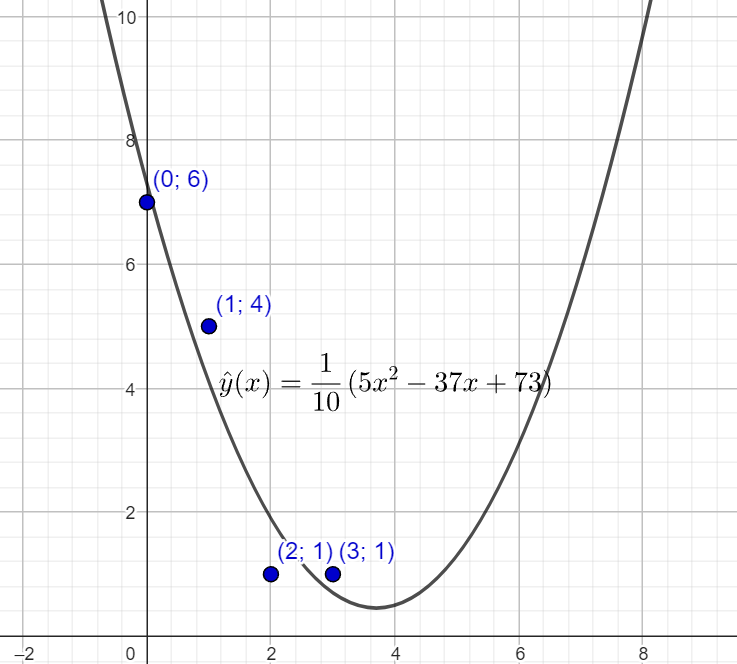
\includegraphics[width=0.5\linewidth]{chapters/nonlinear/sol_pol_1.png}
\end{figure}

\section{Сплайн-регрессия}

Чтобы преодолеть недостатки полиномиальной регрессии, мы можем использовать улучшенный метод регрессии, который вместо построения одной модели для всего набора данных делит набор данных на несколько блоков и подгоняет каждый блок отдельной моделью. Такая техника называется сплайн-регрессией. В этом случае имеется возможность осуществить регрессию сшивкой отрезков (точнее говоря, участков, т. к. они криволинейной формы) нескольких полиномов. Регрессия одним полиномом эффективна, когда множество точек выглядит приблизительно как полином, а регрессия отрезками полиномов оказывается полезной в противоположном случае, например, для функции синуса.

Точки, где происходит разделение, называются узлами. Функции, которые мы можем использовать для моделирования каждого куска/бина, называются кусочными функциями. Существуют различные кусочные функции, которые мы можем использовать для подгонки этих отдельных участков.

Пусть мы разбили $\mathbb{R}$ на $n$ частей, то есть $-\infty=x_0, \,x_1, \, \dots,\, x_{n},\,x_{n+1}=+\infty$. В узлах функции на соседних отрезках могут давать разные значения. Мы либо можем выкалывать узлы и соединять функции на полуинтервалах, тогда $$f(x) = \sum\limits_{i=0}^{n} f_i(x)\mathbb{I}[x_i;\, x_{i+1})$$

Если же мы хотим непрерывности нашей аппроксимирующей функции, то можно соединять функции на отрезках $[x_i+\varepsilon; \, x_{i+1}-\varepsilon]$ при малом $\varepsilon>0$, и затем соединять пары точек вида $(x_i-\varepsilon,\, f_{i-1}(x_i-\varepsilon))$ и $(x_i+\varepsilon,\, f_{i}(x_i+\varepsilon))$ отрезками при $i=\overline{1,n}$.

Когда мы подгоняем сплайн, где мы должны разместить узлы? Одним из потенциальных мест может быть область высокой изменчивости, потому что в этих областях коэффициенты полинома могут быстро меняться. Следовательно, одним из вариантов является размещение большего количества узлов в тех местах, где, по нашему мнению, функция может изменяться наиболее быстро, и размещение меньшего количества узлов в тех местах, где она кажется более стабильной.

Хотя эта опция может работать хорошо, на практике обычно принято размещать узлы равномерно. Один из способов сделать это - указать желаемые степени свободы, а затем заставить программное обеспечение автоматически размещать соответствующее количество узлов в одинаковых квантилях данных.

Другой вариант - опробовать разное количество узлов и посмотреть, какой вариант дает наилучшую кривую.

Более объективный подход заключается в использовании кросс-валидации. С помощью этого метода: мы удаляем часть данных, подгоняем сплайн с определенным количеством узлов к оставшимся данным, а затем используем сплайн, чтобы сделать прогноз для удаленной части данных.

Мы повторяем этот процесс несколько раз, пока каждое наблюдение не будет пропущено хотя один раз, а затем вычисляем общее перекрестное значение RMSE. Эту процедуру можно повторить для разного количества K узлов. Затем выбирается значение K, дающее наименьшее RMSE (среднеквадратическая ошибка).

Сплайновая регрессия часто дает лучшие результаты, чем полиномиальная регрессия. Это связано с тем, что в отличие от полиномов высоких степеней, которые необходимо использовать для получения гибкой подгонки, сплайны обеспечивают гибкость, увеличивая количество узлов, но сохраняя фиксированную степень.


\problem Рассмотрим задачу аппроксимации функции с помощью сплайн-регрессии. Пусть у нас есть набор данных, представляющий собой значения функции \(f(x)\) в определенных точках:

\begin{align*}
x_0 & = 0, \quad f(x_0) = 1 \\
x_1 & = 1, \quad f(x_1) = 2 \\
x_2 & = 2, \quad f(x_2) = 0 \\
x_3 & = 3, \quad f(x_3) = 3 \\
x_4 & = 4, \quad f(x_4) = 2
\end{align*}

Постройте функции кусковой линейной регрессии (линейные сплайны) на отрезках \([x_0, x_1]\), \([x_1, x_2]\), \([x_2, x_3]\) и \([x_3, x_4]\) и соедините их в одну непрерывную функцию.

\solution
1. Отрезок \([x_0, x_1]\):\\
Два известных значения: \(f(0) = 1\) и \(f(1) = 2\). Угловой коэффициент: 
     $\displaystyle     a_0 = \frac{f(1) - f(0)}{x_1 - x_0} = \frac{2 - 1}{1 - 0} = 1.$ Тогда $y_0 = 1 \cdot x + 1 = x + 1.$\\
2. Отрезок \([x_1, x_2]\):\\
     $\displaystyle     a_1 = \frac{f(2) - f(1)}{x_2 - x_1} = \frac{0 - 2}{2 - 1} = -2.$ Тогда $y_0 = -2 x + 4 = -2x + 4.$\\
3. Отрезок \([x_2, x_3]\):\\
       $\displaystyle     a_2 = \frac{f(3) - f(2)}{x_3 - x_2} = \frac{3 - 0}{3 - 2} = 3.$ Тогда $y_0 = 3x - 6 = 3x-6.$\\
4. Отрезок \([x_3, x_4]\):
    $\displaystyle     a_3 = \frac{f(4) - f(3)}{x_4 - x_3} = \frac{2 - 3}{4 - 3} = -1.$ Тогда $y_0 = -1\cdot x + 6 = -x + 6.$

Наконец, мы можем пострить нашу итоговую функцию (сплайн-регрессию):
\[
\hat{f}(x) =
\begin{cases}
x + 1, & x \in [0, 1] \\
-2x + 4, & x \in [1, 2] \\
3x - 6, & x \in [2, 3] \\
-x + 6, & x \in [3, 4]
\end{cases}
\]






\section*{Методы Ньютона-Рафсона, Ньютона-Гаусса}

Мы уже познакомились с задачами линейной регрессии и обсудили несколько методов их решения. Но что делать если задача нелинейна? Оказывается, что идея локальной линейности гладкой функций позволяет свести задачу к более простому. На этой идее основаны методы второго порядка - Ньютона-Рафсона и Ньютона-Гаусса.

\subsection*{Метод Ньютона-Рафсона}

Начнем немного сдалека, а именно рассмотрим задачу поиска нуля $a$ функций $f(x)$. Пусть мы находимся в точке $a^{0}$ и хотим найти такое приращение $h$, чтобы приблизиться к точке $a$: $a^{0} + h \approx a$. Применим разложение в ряд:

\begin{gather*}
    f(a^{0} + h) = f(a^{0}) + f'(a^{0})h + o(h)\\[1em]
    f(a^{0} + h) \approx f(a) = 0 \Rightarrow f(a^{0}) + f'(a^{0})h \approx 0
\end{gather*}

Откуда

\[
h \approx - \frac{f(a^{0})}{f'(a^{0})}
\]

Значит, для поиска нуля выпуклой функций \( f \) можно применить следующий итеративный метод:

\[
a^{k + 1} = a^{k} - \frac{f(a^{k})}{f'(a^k)}
\]

Вернемся к начальной задаче:

\begin{itemize}
    \item обучающая выборка \( X^{l} = (x_{i}, y_{i}) \), где \( x_{i} \) - вектор признаков \( i \)-го объекта
    \item \( y_{i} = y(x_{i}),\quad y: X \to Y \) - неизвестная регрессионная зависимость
    \item \( f(x, \alpha) \) - нелинейная модель регрессии, где \( \alpha \) - вектор параметров
\end{itemize}

Хотим решить задачу оптимизации методом наименьших квадратов:

\[
Q(\alpha, X^{l}) = \sum\limits_{i = 1}^{l}\left(f(x_{i}, \alpha) - y_{i} \right)^{2} \to \min_{\alpha}
\]

Функция потерь \( Q(\alpha, X^{l}) \) выпукла и гладкая в предположений гладкости \( f(\alpha, x) \), поэтому для ее минимизаций достаточно найти нуль производной (градиента). Применяя рассуждения выше и опустив технические детали, получим следующий итерационный процесс:

\[
\alpha^{k + 1} = \alpha^{k} - h_{k}\left(Q''( \alpha^{k} )\right)^{-1} Q'(\alpha^{k})
\]

где \( Q'( \alpha^{k} ) \), \( Q''(\alpha^{k} ) \) - градиент и гессиан \( Q \) в точке \( \alpha^{k} \) соответственно, \( h_{k} \) - величина шага.
\subsection*{Метод Ньютона-Гаусса}

Подсчет обратного гессиана на каждой итерации может дорого обходиться, поэтому посмотрим на полученный выше результат с другой стороны. Для этого запишем несколько формул:

Компоненты градиента \( Q(\alpha, X^{l}) \):

\[
\frac{\partial Q(\alpha, X^{l})}{\partial\alpha_{j}} = 2 \sum\limits_{i = 1}^{l} \left(f(x_{i}, \alpha) - y_{i} \right)\frac{\partial f(x_{i}, \alpha)}{\partial\alpha_{j}}
\]

Компоненты гессиана:

\[
\frac{\partial Q(\alpha, X^{l})}{\partial\alpha_{j}\partial\alpha_{k}} = 2\sum\limits_{i = 1}^{l}\frac{\partial f(x_{i}, \alpha)}{\partial\alpha_{j}}\frac{\partial f(x_{i}, \alpha)}{\partial\alpha_{k}} - 2\sum\limits_{i = 1}^{l}\left(f(x_{i}, \alpha) - y_{i}\right)\frac{\partial^2 f(x_{i}, \alpha)}{\partial\alpha_{j}\partial\alpha_{k}}
\]

Второе слагаемое в формуле выше полагается равным нулю, исходя из линейной аппроксимации функций \( f \). Введем следующие обозначения и перепишем формулу итерации метода Ньютона-Рафсона:

\begin{gather*}
    F_{k} = \left( \frac{\partial f}{\partial\alpha_{j}}(x_{i}, \alpha^{k}) \right)_{i, j}\\[1em]
    f_{k} = \left( f(x_{i}, \alpha^{k}) \right)_{i}
\end{gather*}

Получим:

\[
\alpha^{k + 1} = \alpha^{k} - h_{k}(F_{k}^{T}F_{k})^{-1}F_{k}^{T}(f_{k} - y)
\]

Положив \( \theta = (F_{k}^{T}F_{k})^{-1}F_{k}^{T}(f_{k} - y) \), получим решение задачи линейной регрессии, где новые ответы обучающей выборки -- \( \left(f_{k} - y \right) \), с новой матрицей признаков~--~\( F_{k} \). Таким образом, каждый шаг метода Ньютона-Гаусса сводится к задаче линейной регрессии. 

\section*{Задачи}

\subsection*{Задача 1: Локальная сходимость}

Найдите допустимые значения начального приближения для поиска нуля функции \( f(x) = \frac{x}{\sqrt{1 + x^{2}}} \).

\textbf{Решение:}

Нуль функции \( f \) достигается в точке \( a = 0\). Посчитаем производную \( f \):

\[
f'(x) = \left(\frac{x}{\sqrt{1 + x^{2}}}\right)' = \frac{1}{\sqrt{1 + x^{2}}} - x\cdot\frac{2x}{2(1 + x^{2})^{3/2}} = \frac{1}{(1 + x^{2})^{3/2}}
\]

Распишем формулу итерации метода Ньютона:

\[
a^{k + 1} = a^{k} - \frac{f(a^{k})}{f'(a^{k})} = -(a^{k})^3
\]

Отсюда видно, что сходимость есть при \( |a^{0}| < 1 \). Делаем вывод о важности выбора начального приближения в данном методе.

\subsection*{Задача 2: Квадратичная задача}

Как сработает метод Ньютона-Рафсона для поиска минимума задачи \( f(x)~=~x^{T}Ax + bx + c\),  где $x, b \in \mathbb{R}^{n}$, $A$ - симметричная, положительно определенная матрица.

\textbf{Решение:}

Для поиска минимума нужно найти нуль градиента. Это и будет точкой минимума, так как задача выпукла.
Посчитаем градиент и гессиан:

\begin{gather*}
    \nabla f(x) = Ax + b\\[1em]
    \nabla^{2} f(x) = A
\end{gather*}

Пусть \( x^{0} \) начальная точка. Применяя формулу из метода Ньютона-Рафсона получим:

\[
x^{1} = x^{0} - \left(\nabla^{2} f(x^{0})\right)^{-1}\nabla f(x^{0}) = x^{0} - A^{-1}\left(Ax^{0} + b\right) = -A^{-1}b
\]

но с другой стороны, градиент обращается в нуль в этой точке:

\[
\nabla f(x) = 0 = Ax + b \Rightarrow x = -A^{-1}b
\]


Значит для квадратичной задачи данный метод дает ответ за 1 шаг. Вообще говоря, если функция $\mu$-выпукла и имеет $M$-липшецевый гессиан, то скорость сходимости локально квадратична.

\subsection*{Задача 3: Система уравнений}

Составьте алгоритм решения следующей системы с помощью методов второго порядка:

\[
\begin{cases}
x^{2} + y^{2} = 4\\
y = e^{x}
\end{cases}
\]

\textbf{Решение:}

Нужно найти нули следующей функции от двух переменных
\[
F(x, y) = 
\begin{pmatrix}
x^{2} + y^{2} - 4 \\
y - e^x
\end{pmatrix}
\]

Запишем итерацию метода Ньютона-Рафсона:

\[
x^{k + 1} = x^{k} - J_{F}(x^{k})^{-1}F(x^{k})
\]

Его можно записать как:

\[
J_{F}(x^{k})(x^{k + 1} - x^{k}) = -F(x^{k})
\]

Посчитаем матрицу якоби функции $F$:

\[
J_{F}(x) = 
\begin{pmatrix}
2x   & 2y \\
-e^x & 1
\end{pmatrix}
\]

Тогда на каждом шаге нужно решить следующую систему:
\[
\begin{pmatrix}
    2x^{k} & 2(y^{k})^{2} \\
    -e^{x^{k}} & 1 
\end{pmatrix}
\begin{pmatrix}
    c_{1}^{k + 1}  \\
    c_{2}^{k + 1}
\end{pmatrix} 
=
\begin{pmatrix}
    (x^{k})^2 + (y^{k})^2 - 4\\
    (y^{k}) - e^{x^{k}}
\end{pmatrix} 
\]

где \( c^{k + 1} = -(x^{k + 1} - x^{k})\). Тогда для решения данной задачи нужно взять начальную точку и проделать несколько итераций описанных уравнениями выше.

\section{Обобщенная аддитивная модель}

Обобщённые аддитивные модели (Generalized Additive Models, GAM) предоставляют подход к моделированию данных, который обобщает линейную регрессию за счёт введения нелинейных преобразований отдельных признаков. Основная цель GAM — построить модель, в которой линейная структура сохраняется, но при этом каждый признак может вносить свой вклад через нелинейную функцию преобразования.

\
\textbf{Пример: прогнозирование стоимости недвижимости}

Стоимость квартиры может зависеть от множества факторов: площади, количества комнат, наличия балкона, удалённости от метро и других. Некоторые признаки, такие как площадь, являются числовыми, другие, например наличие балкона, — бинарными. Возникает вопрос, как корректно обработать такой признак, как расстояние до метро. Интуитивно понятно, что стоимость квартиры снижается с увеличением расстояния, но эта зависимость может быть нелинейной. Простое включение признака в линейную модель может не учесть этой особенности, так как предполагает постоянный коэффициент (обычно отрицательный) для расстояния до метро.

Таким образом, чтобы учесть сложную зависимость, расстояние до метро можно преобразовать через некоторую нелинейную функцию $\phi(x)$, которая будет отражать реальный характер этой связи. GAM позволяет обучить эту функцию непосредственно из данных.


Обобщённая аддитивная модель представляется в виде:
$$f(x, \alpha) = \sum_{j=1}^{n}\phi_j(f_j(x), \alpha_j)$$
В частности, при $\phi_j(f_j(x), \alpha_j) = \alpha_jf_j(x)$ это линейная модель.

Идея состоит в том, чтобы поочередно обучать параметры $\phi_j$ при фиксированных остальных. На каждом шаге получается задача обучения одномерной модели регрессии. Также добавлен регуляризатор $R(\alpha_j)$.
$$\sum_{i=1}^{l}(\phi_j(f_j(x_i), \alpha_j) - (y_i - \sum_{k \neq n}\phi_k(f_k(x_i), \alpha_k))^2 + tR(\alpha_i) \to min_{a_i}$$

$R$ - регуляризатор гладкости:  

$$R(\alpha_i) = \int(\phi_j^{''}(\zeta, \alpha_j)^2d\zeta$$

Для оптимизации регуляризаторов используют такие методы как сплайны или ядерное сглаживание 


\subsection{Задача 1}
Объясните, зачем в обобщённых аддитивных моделях (GAM) используется регуляризация для функции $\phi_j(x)$:
\flushleft
\begin{enumerate}
\item Регуляризация предотвращает переобучение модели, штрафуя за чрезмерно сложные функции $\phi_j(x)$. 

\item Регуляризация ускоряет процесс обучения модели, уменьшив количество данных, которые необходимо обработать.
\item Регуляризация заставляет модель использовать только линейные функции для преобразования признаков.
\item Регуляризация повышает точность прогноза, исключая менее важные признаки из модели.
\begin{description}
\end{description}
\end{enumerate}
Ответ: 1

\subsection{Задача 2}

В обобщённой аддитивной модели (GAM) имеется следующая формула:

\[
y = \alpha_0 + \sum_{j=1}^{n} \phi_j(x_j) + \epsilon
\]

где \( \phi_j(x_j) \) — это нелинейные функции преобразования признаков.


\textbf{Вопрос:} Если одна из функций преобразования \( \phi_j(x_j) \) — это просто линейная функция, то какую роль она выполняет в модели? И что произойдёт, если такую функцию исключить из модели?

\textbf{Решение:}
Тогда это эквивалентно линейной регрессии. Если исключить признак из модели, то его влияние будет упущено, что пможет привести к потери важной информации.





\subsection{Задача 3}
Для данных с признаками:
\[
x_1 (\text{площадь}),x_2 (\text{количество комнат}),x_3 (\text{расстояние до метро})
\]
известна модель:
\[
y = 50 + \phi_1(x_1) + \phi_2(x_2) + \phi_3(x_3) + \varepsilon,
\]
где \(x_1 \sim U(20, 100)\), \(x_2 \sim \{1, 2, 3, 4\}\), \(x_3 \sim U(0.5, 10)\).

Постройте GAM для оценки $\phi_i(x)$ и оцените, какой признак вносит наибольший вклад в стоимость.





\section{Backfitting}

На практике встречаются задачи, в которых использование линейных моделей необосновано, но и не удаётся предложить явную нелинейную модель. В таком случае строится модель вида

$$\displaystyle y(x)=f(x,\theta)=\sum_{j=1}^m\theta_j \phi_j(x_j),$$

где $x$ ~--- объект, $x_j$ ~--- признаки объекта, $\phi_j:\mathbb{R}\rightarrow \mathbb{R}$ ~--- нелинейные в общем случае преобразования.

Задача состоит в том, чтобы одновременно подбирать коэффициенты модели $\theta_j$ и неизвестные преобразования $\phi_j$.

Суть метода backfitting (метод настройки с возвращением) заключается в чередовании оптимизации коэффициентов $\theta_j$ при постоянных $\phi_j$ методами линейной регрессии, и оптимизации преобразований $\phi_j$ при постоянных коэффициентах $\theta_j$. 

Для минимизации используется сумма квадратов ошибок на всех объектах:

$Q(\theta, \phi) = \displaystyle \sum_{i=1}^l \left( y(x_i) - y_i \right)^2 = \sum_{i=1}^l \left( \sum_{j=1}^m \theta_j \phi_j(X_{ij}) - y_i \right)^2 $

Здесь $X$ ~--- матрица признаков.

\subsection{Алгоритм backfitting}
\begin{algorithmic}
\State $\phi_j(t) \equiv t$ ~--- изначальное приближение линейными функциями
\While{($Q$ уменьшается)} 
    \State $\theta \gets \text{argmin}_{\theta}Q(\theta, \phi_j)$ ~--- при фиксированных $\phi_1,\dots, \phi_k$
    \For{$j=1\dots m$}
        \State $\displaystyle r_i = y_i - \sum_{k\neq j} \theta_k \phi_k(X_{ik})$
        \State $r_i$ ~--- ошибка модели на $i$ объекте, без учёта $j$ признака
        \State $\displaystyle\phi_j \gets \text{argmin}_{\phi} \sum_{i=1}^l \left( \theta_j \phi(X_{ij}) - r_i \right)^2$ ~--- при $\theta_j=const$
    \EndFor
\EndWhile 
\end{algorithmic}

Оптимизация по коэффициентам $\theta \gets \text{argmin}_{\theta}Q(\theta, \phi_j)$ выполняется методами линейной регрессии, такими как стохастический градиентный спуск.

Оптимизация по функции $\phi_j$ выполняется одномерными методами, такими как ядерное сглаживание.

Варианты дальнейшего развития метода:
\begin{itemize}
    \item [1.] Во внутреннем цикле выбирать индексы $j$ не в фиксированном порядке, а в первую очередь оптимизировать дающие наибольший вклад в $Q$.
    \item [2.] Регуляризация $Q$ по параметрам $\theta$ и по сложности функций $\phi$.
\end{itemize}

\subsection{Задача}

Если матрица признаков $X$ разреженная, с какой проблемой можно столкнуться, применяя алгоритм backfitting, и как её решить?

Решение: если каждая из функций $\phi_j$ вызывается лишь на небольшом наборе аргументов, то её значения на них могут быть почти независимы (если модель $\phi$ достаточно сложна, например, полином высокого порядка), и случится переобучение. Варианты решения: большая константа регуляризации по сложности функций $\phi$; ограничить $\phi$ более простым классом функций (например, только квадратичные функции вместо полиномов); расширить матрицу признаков несколькими простыми нелийными преобразованиями ($\sin x$, $x^2$...) и использовать методы линейной регрессии.

\section{Метод наименьших квадратов с итеративным пересчётом весов (IRLS)}

\textbf{Метод наименьших квадратов с итеративным пересчётом весов} (Iteratively Reweighted Least Squares) применяется для решения задач оптимизации. В частности, применение метода Ньютона-Рафсона к задаче \textit{Логистической регрессии} сводится к \textbf{IRLS}.

Напомним постановку задачи линейной регрессии. Будем искать приближенное решение системы:

\[ \begin{bmatrix} 
    a_{11} & a_{12} & \dots  & a_{1N} \\
    \vdots & \vdots & \ddots & \\
    a_{M1} & \dots  & \dots  & a_{MN}
\end{bmatrix} \begin{bmatrix} 
    x_{1} \\
    \vdots \\
    x_{M} \\ 
\end{bmatrix}
=
\begin{bmatrix} 
    y_{1} \\
    \vdots \\
    y_{M} \\
\end{bmatrix} \]

То же самое в матричных обозначениях:

\[
    \boldsymbol{A} \boldsymbol{x} = \boldsymbol{y}
\]

Поставим задачу минимизировать норму вектор ошибки (невязки):

\[
    \boldsymbol{e} = \boldsymbol{A} \boldsymbol{x} - \boldsymbol{y} 
\]

В качестве нормы возьмем p-норму: $||\boldsymbol{e}||_p = \left( \sum_i |e_i|^p \right)^{1/p}$. Как известно, если методом наименьших квадратов можно аналитически найти решение, минимизирующее Евклидову норму вектора невязки (root-mean-squared error) $\sqrt{\boldsymbol{e}^T \boldsymbol{e}}$. Покажем как можно построить итеративный подход, использующий результаты для взвешенного метода наименьших квадратов, для нахождения оптимального решения для $l_p$ нормы.

\subsection{Взвешенные метод наименьших квадратов}

Для построения IRLS нужно сперва вспомнить основные результаты взвешенной модификации МНК. Добавим в Евклидову норму веса для каждой компоненты вектора $\boldsymbol{x}$ и будем минимизировать норму:

\[
    \boldsymbol{||W e||_2^2} = \sum_i w_i^2 e_i^2 = \boldsymbol{e}^T \boldsymbol{W}^T \boldsymbol{W} \boldsymbol{e} 
\]

\[
    \boldsymbol{W} = diag(w_1, w_2, \dots, w_M)
\]

$\boldsymbol{W}$ - диагональная матрица ненулевых весов. Легко видеть, что такое взвешивание соответствует линейному преобразованию растяжения с коэффициентами $w_1, w_2, \dots w_M$. Для переопределенной системы решение с минимальной взвешенной нормой оказывается равным:

\[
    \boldsymbol{x} = \left[ \boldsymbol{A^T W^T W A} \right]^{-1} \boldsymbol{A^T W^T W y}
\]

\subsection{Алгоритм \textbf{IRLS}}

Поиск минимума $||\boldsymbol{e}||_p = \left( \sum_i |e_i|^p \right)^{1/p}$ сводится к итеративному алгоритму, где на каждом шаге применяется взвешенный МНК. Набор весов $w_1, w_2, \dots, w_M$ пересчитывается на каждой итерации $n$.

\[
||e(n +1)||_p = \left( \sum_i w_i^2(n) |e_i(n)|^2 \right)^{1/2}
\]

\[
w_i(n) = e_i(n)^{\frac{p - 2}{2}}
\]

Начальные веса $w_1, w_2, \dots, w_M$ берутся единичными, т.е. для первой итерации используется в качестве приближения используется стандартный МНК.

\subsection{Задачи}

\subsubsection{Задача 1: WLS}

Получить оптимальное решение для переопределенной системы с взвешенной нормой. \\

\textbf{Решение:}

Вспомним результат обычного МНК:

\[
    \boldsymbol{A} \boldsymbol{x} = \boldsymbol{y}
\]

\[
    \boldsymbol{x} = \left[\boldsymbol{X^T X}\right]^{-1} \boldsymbol{X y}
\]

Домножая слева на $\boldsymbol{W}$ получим: $\boldsymbol{W} \boldsymbol{A} \boldsymbol{x} = \boldsymbol{W} \boldsymbol{y}$. Получаем исходную задачу МНК с матрицей $\boldsymbol{W} \boldsymbol{A}$ и правой частью $\boldsymbol{W} \boldsymbol{y}$. Отсюда сразу получается ответ:

\[
    \boldsymbol{x} = \left[ \boldsymbol{A^T W^T W A} \right]^{-1} \boldsymbol{A^T W^T W y}
\]

\subsubsection{Задача 2: Пример IRLS для $l_1$}

Реализовать IRLS и применить его для нахождения линейной модели по набору точек $x, y$: $(1, 2), (2, 3), (4, 6)$. Применить реализованный метод и убедиться, чтобы итеративный метод сходится к $3 / 2$ для $p = 1$ (норма $l_1$) и к $32 / 21$ для $p = 2$.

\subsubsection{Задача 3: Зависимость весов для $l_p$}

Обосновать выбор $w_i(n) = e_i(n)^{\frac{p - 2}{2}}$, считая что итеративный метод сходится.

\subsubsection{Задача 4: Логистическая регрессия как IRLS}

Показать, как применение метода Ньютона-Рафсона к логистической регрессии приводит к IRLS.

\textbf{Решение:}

\textit{см. раздел про логистическую регрессию}

\section{Гауссовы процессы для задачи классификации. Применение Лапласовой аппроксимации для Гауссовсого процесса}

В вероятностном подходе к задаче классификации, наша цель — смоделировать апостериорные
вероятности целевой переменной для нового входного вектора, учитывая набор обучающих
данных. Эти вероятности должны лежать в интервале (0,1). Проблема в том, что модель гауссовского процесса делает предсказание для всей действительной оси. Однако мы можем легко
адаптировать гауссовские процессы к задачам классификации, преобразуя вывод
гауссовских процессов с помощью подходящей нелинейной функции активации.

Рассмотрим сначала задачу классификации с целевой переменной $y \in \{0,1\}$. Если мы определим гауссовский процесс c функцией $a(\mathbf{x})$, а затем преобразуем функцию с помощью сигмоиды $z=\sigma(a)$, заданной формулой $\frac{1}{1+exp(-a)}$, то мы получим негауссовский
стохастический процесс c функциями $z(x)$, где $z \in \{0,1\}$.

Обозначим входные данные обучающей выборки как $x_1,...,x_N$ с соответствующими
наблюдаемыми целевыми переменными $\mathbf{y} =(y_1,...,y_N)^T$. Мы также рассматриваем одну контрольную точку
$x_{N+1}$ с целевым значением $y_{N+1}$. Наша цель — определить предсказательное распределение
$p(y_{N+1}|\mathbf{y})$, где зависимость от входных переменных оставлена неявной. Для этого мы строим гауссовский процесс по вектору $\mathbf{a}_{N+1}$, который имеет компоненты $a(\mathbf{x}_1),...,a(\mathbf{x}_{N+1})$. Это, в свою очередь, определяет негауссовский процесс по $y_{N+1}$,
и, условно оценивая по обучающим данным $y_N$, мы получаем требуемое предсказательное распределение. Гауссовский процесс для $a_{N+1}$ принимает вид
\[ p(\mathbf{a}_{N+1})=N(\mathbf{a}_{N+1}|\mathbf{0},\mathbf{C}_{N+1})\]

По численным причинам удобно ввести шумоподобный член, определяемый
параметром $\nu$. Шумоподобный член нам нужен для того, чтобы ковариационная матрица была положительно определена. Таким образом,
Ковариационная матрица $\mathbf{C}_{N+1}$ состоит из элементов определяемых следующим уравнением $C(\mathbf{x}_n,\mathbf{x}_m)=k(\mathbf{x}_n,\mathbf{x}_m)+\nu\delta_{nm}$
где $k(\mathbf{x}_n,\mathbf{x}_m)$ — любая положительно полуопределенная функция ядра вида: $\phi(x_n)^T\phi(x_m)$, а значение $\nu$ обычно фиксируется заранее. Мы предположим, что
функция ядра $k(\mathbf{x},\mathbf{x}^{\prime})$ определяется вектором $\mathbf{\theta}$ параметров. В дальнейшем мы узнаем, как можно узнать вектор $\mathbf{\theta}$ из обучающих данных.

Для задачи классификации с двумя классами достаточно предсказать $p(y_{N+1} =1|y_{N})$, поскольку
значение $p(y_{N+1} =0|y_{N})$ тогда задается как $1-p(y_{N+1} =1|y_{N})$. Тогда требуемое
предсказательное распределение задается как
\begin{equation}
p(y_{N+1} =1|\mathbf{y}_{N})= \int p(t_{N+1} =1|a_{N+1})p(a_{N+1}|\mathbf{y}_N)da_{N+1},
\end{equation}
где $p(t_{N+1} =1|a_{N+1})=\sigma(a_{N+1})$. Этот интеграл аналитически неразрешим. Однако в вычислении этого предсказательного распределения нам поможет аппроксимация Лапласа, которую мы и рассмотрим.

\subsection{Лапласова аппроксимация}
Воспользуемся теоремой Байеса, получим следующую цепочку равенств
\begin{equation}
\label{integral}
\begin{split}
&p(a_{N+1}|\mathbf{y}_{N}) = \int p(a_{N+1},\mathbf{a}_{N}|\mathbf{y}_N)d\mathbf{a}_{N}
= \frac{1}{p(\mathbf{y}_N)} \int p(a_{N+1},\mathbf{a}_{N})p(\mathbf{y}_{N}|a_{N+1},\mathbf{a}_{N})da_{N}= \\
&=\frac{1}{p(\mathbf{y}_{N})} \int p(a_{N+1}|\mathbf{a}_{N})p(\mathbf{a}_{N})p(\mathbf{y}_{N}|\mathbf{a}_{N})d\mathbf{a}_{N}= \int p(a_{N+1}|\mathbf{a}_{N})p(\mathbf{a}_{N}|\mathbf{y}_{N})d\mathbf{a}_{N}
\end{split}
\end{equation}
где мы использовали формулу $p(\mathbf{y}_{N}|a_{N+1},\mathbf{a}_{N})=p(\mathbf{y}_{N}|\mathbf{a}_{N})$. 
Условное распределение $p(a_{N+1}|\mathbf{a}_{N})$ получается использованием формулы  $m(x_{N+1}) = \mathbf{k}^T\mathbf{C}^{-1}_N\mathbf{y}$ и формулы для дисперсии $\sigma^2(x_{N+1}) = c-\mathbf{k}^T\mathbf{C}^{-1}_N\mathbf{k}$. Таким образом мы получаем
\[
\label{condition}
p(a_{N+1}|\mathbf{a}_{N})=N(a_{N+1}|\mathbf{k}^T\mathbf{C}^
{-1}_N\mathbf{a}_{N},c-\mathbf{k}^T\mathbf{C}^{-1}_N\mathbf{k})\]

Поэтому мы можем оценить интеграл в \ref{integral}, найдя приближение Лапласа
для распределения $p(\mathbf{a}_{N}|\mathbf{y}_{N})$, а затем используя стандартную формулу для
свертки двух гауссовых распределений.

$p(\mathbf{a}_{N})$ задается гауссовым процессом c нулевым средним и ковариационной матрицей $\mathbf{C}_{N}$, $p(\mathbf{y}_{N}|\mathbf{a}_{N})$ задается как
\[
p(\mathbf{y}_{N}|\mathbf{a}_{N})=\displaystyle \prod_{n=1}^{N}\sigma(a_{N})^{y_n}(1-\sigma(a_{n}))^{1-y_n} =
\displaystyle \prod_{n=1}^{N} e^{a_ny_n}\sigma(-a_n)\]

Затем мы получаем аппроксимацию Лапласа разложением Тейлора логарифма $p(\mathbf{a}_{N}|\mathbf{y}_N)$, который, с точностью до аддитивной константы, задается следующей формулой
\begin{equation}
\label{PSI}
 \Psi(\mathbf{a}_N) = \ln p(\mathbf{a}_{N})+\ln p(\mathbf{y}_N|\mathbf{a}_N)
 = -\frac{1}{2}\mathbf{a}^{T}_N\mathbf{C}^{-1}_N \mathbf{a}_N-\frac{N}{2} \ln(2\pi)-\frac{1}{2}\ln|\mathbf{C}_N|+\mathbf{y}^T_N\mathbf{a}_N-\displaystyle \sum^{N}_{n=1}\ln(1+e^{a_n})+const
\end{equation}

Сначала нам нужно найти моду апостериорного распределения, и для этого требуется вычислить градиент $\Psi(a_N)$, который задаётся выражением:
\[
\nabla \Psi(\mathbf{a}_N) = \mathbf{y}_N - \sigma_{N} - \mathbf{C}_{N}^{-1}\mathbf{a}^N
\]
где $\mathbf{\sigma}_N$ — вектор с элементами $\sigma(a_n)$. \\

\textbf{Задача 1:}
Почему мы не можем найти моду, просто приравнивая этот градиент к нулю? 

\textbf{Решение:}
Потому что $\mathbf{\sigma}_N$ нелинейно зависит от $a_N$ 

Мы прибегаем к итеративной схеме, основанной на методе Ньютона-Рафсона, что приводит к итеративному взвешенному методу наименьших квадратов (IRLS). Это требует вычисления вторых производных $\Psi(\mathbf{a}_N)$, которые нам также необходимы для лапласовского приближения, и которые задаются выражением:
\[
\nabla \nabla \Psi(\mathbf{a}_N) = -\mathbf{W}_{N} - \mathbf{C}_{N}^{-1} 
\]
Мы видим, что гессиан $A=-\nabla \nabla \Psi(a_N)$ является положительно определённой матрицей, и поэтому апостериорное распределение $p(a_N|y_N)$ является лог-выпуклым и, следовательно, имеет единственную моду, которая является глобальным максимумом.

\textbf{Задача 2:}
Докажите, что гессиан $A=-\nabla \nabla \Psi(a^N)$ является положительно определённой матрицей


\textbf{Решение:}
$\mathbf{W}_{N}$ — диагональная матрица с элементами $\sigma(a_n)(1-\sigma(a_n))$, так как $\frac{d\sigma}{da}=\sigma(1-\sigma)$. Заметим, что эти диагональные элементы лежат в диапазоне $(0, 1/4)$, и, следовательно, $\mathbf{W}_{N}$ является положительно определённой матрицей. Поскольку $\mathbf{C}_N$ (и, следовательно, её обратная матрица) является положительно определёнными по построению. Таким образом мы видим, что гессиан $\mathbf{A}=-\nabla \nabla \Psi(\mathbf{a}_N)$ является положительно определённой матрицей.


Однако апостериорное распределение не является гауссовским, поскольку гессиан является функцией $\mathbf{a}_N$.
Используя формулу Ньютона-Рафсона, итерационное уравнение для $a_N$ имеет вид:
\[
\mathbf{a}_N^{new} = \mathbf{C}_N(\mathbf{I} + \mathbf{W}_N\mathbf{C}_N)^{-1}(\mathbf{y}_N-\mathbf{\sigma}_N+\mathbf{W}_N\mathbf{a}_N) 
\]
Эти уравнения итерируются до тех пор, пока не сойдутся к модe, которую мы обозначаем как $\mathbf{a}_N^{\star}$. На этой моде градиент $\nabla \Psi(\mathbf{a}_N)$ занулится, и, следовательно, $a_N^{\star}$ будет удовлетворять уравнению:
\begin{equation}
\label{star}
\mathbf{a}_N^{\star} = \mathbf{C}_N(\mathbf{y}_N - \mathbf{\sigma}_N) 
\end{equation}
Как только мы нашли моду $a_N^{\star}$ апостериорного распределения, мы можем вычислить гессиан, заданный выражением:
\[
\mathbf{H} = \nabla \nabla \Psi(\mathbf{a}_N) = \mathbf{W}_N+\mathbf{C}_N^{-1} 
\]
где элементы $\mathbf{W}_N$ вычисляются с помощью $\mathbf{a}_N^{\star}$. Это определяет нашу гауссову аппроксимацию к апостериорному распределению $p(\mathbf{a}_N|\mathbf{y}_N)$, задаваемую выражением:
\[
q(a_N) = N(\mathbf{a}_N|\mathbf{a}_N^{\star}, \mathbf{H}^{-1}) 
\]
Теперь мы можем объединить это с \ref{condition} и, следовательно, вычислить интеграл \ref{integral}. Поскольку это соответствует линейной гауссовской модели, мы можем использовать следующую формулы:
\[
\mathbb{E}[a_{N+1}|\mathbf{y}_N] =\mathbf{k}^T(\mathbf{y}_N - \mathbf{\sigma}_N) 
\]
\[
var[a_{N+1}|\mathbf{y}_N] = c-\mathbf{k}^T(\mathbf{W}_N^{-1} + \mathbf{C}_N)^{-1}\mathbf{k} 
\]
Теперь, когда у нас есть гауссово распределение для $p(a_{N+1}|\mathbf{y}_{N})$, мы можем аппроксимировать интеграл \ref{integral}, используя формулу.
\[
\int \sigma(a)N(a|\mu,\sigma^{2})da\simeq \sigma(\kappa(\sigma^{2})\mu)
\]

Нам также нужно определить параметры $\mathbf{\theta}$ функции ковариации. Один из возможных подходов — максимизировать функцию правдоподобия, заданную как $p(\mathbf{y}_N|\mathbf{\theta})$, для чего нам нужны выражения для логарифма функции правдоподобия и её градиента. При желании можно также добавить подходящие регуляризирующие члены, что приведёт к решению с помощью метода максимального правдоподобия со штрафом. Функция правдоподобия определяется выражением:
\[
p(\mathbf{y}_N|\mathbf{\theta}) = \int p(\mathbf{y}_N|\mathbf{a}_N)p(\mathbf{a}_N|\mathbf{\theta})d\mathbf{a}_N 
\]
Этот интеграл аналитически невычислим, поэтому снова используем лапласовское приближение. Используя формулу, 
\[
\int f(\mathbf{z})d\mathbf{z} \simeq f(\mathbf{z}_0)\frac{(2 \pi)^{N/2}}{|\mathbf{A}|^{1/2}}
\]
где $\mathbf{A}=-\nabla \nabla \ln f(\mathbf{z})|_{z=z_0}$ - $N \times N$-матрица мы получаем следующее приближение для логарифма функции правдоподобия:
\begin{equation}
\label{log}
\ln p(\mathbf{y}_N|\mathbf{\theta}) = \Psi(\mathbf{a}_N^{\star}) - \frac{1}{2}\ln|\mathbf{W}_N+ \mathbf{C}_N^{-1}| + \frac{N}{2}\ln(2\pi) 
\end{equation}
где $\Psi(\mathbf{a}_N^{\star}) = \ln p(\mathbf{a}_N^{\star}|\mathbf{\theta}) + \ln p(\mathbf{y}_N|\mathbf{a}_N^{\star})$. Нам также нужно вычислить градиент $\ln p(\mathbf{y}_N|\mathbf{\theta})$ c учётом вектора параметров $\mathbf{\theta}$. Заметим, что изменение $\theta$ вызовут изменения $a_N^{\star}$, что приведёт к появлению дополнительных слагаемых в градиенте. Таким образом, когда мы дифференцируем \ref{log} по $\theta$, мы получаем два набора слагаемых, первый возникает из-за зависимости ковариационной матрицы $C_N$ от $\theta$, а второй — из-за зависимости $a_N^{\star}$ от $\theta$.

Слагаемые, возникающие из-за явной зависимости от $\theta$, могут быть найдены с помощью \ref{PSI} вместе с формулами: 
\begin{equation}
\label{odin}
    \frac{\partial}{\partial x}(\mathbf{A}^{-1})=-\mathbf{A}^{-1}\frac{\partial \mathbf{A}}{\partial x}\mathbf{A}^{-1}
\end{equation}
и 
\begin{equation}
\label{dwa}
    \frac{\partial}{\partial x}\ln(|\mathbf{A}|)=Tr(\mathbf{A}^{-1}\frac{\partial \mathbf{A}}{\partial x})
\end{equation} 
и задаются выражением:
\[
\label{urav1}
\frac{\ln p(\mathbf{y}_N|\theta)}{\partial \theta_j} = \frac{1}{2}a_N^{\star T}\mathbf{C}_N^{-1}\frac{\partial \mathbf{C}_N}{\partial \theta_j}\mathbf{C}_N^{-1}a_N^{\star} - \frac{1}{2}Tr[(\mathbf{I} + \mathbf{C}_N\mathbf{W}_N)^{-1}\mathbf{W}_N\frac{\partial \mathbf{C}_N}{\partial \theta_j}] 
\]
Для вычисления слагаемых, возникающих из-за зависимости $\mathbf{a}_N^{\star}$ от $\mathbf{\theta}$, заметим, что лапласовское приближение построено таким образом, что $\Psi(a_N)$ имеет нулевой градиент, если $\mathbf{a}_N=\mathbf{a}_N^{\star}$, Следовательно $\Psi(a_N^{\star})$ не даёт вклада в градиент. Отсюда получаем:
\[
\label{urav2}
-\frac{1}{2} \displaystyle \sum_{i=1}^{N} \frac{\partial \ln|\mathbf{W}_N + \mathbf{C}_N^{-1}|}{\partial a_n^{\star}})\frac{\partial a_n^{\star}}{\partial \theta_j} = -\frac{1}{2} \displaystyle \sum_{i=1}^N [\mathbf{I} + \mathbf{C}_N\mathbf{W}_N)^{-1}\mathbf{C}_N]_{nn} \sigma_{n}^{\star}(1-\sigma_{n}^{\star})(1-2\sigma_{n}^{\star})\frac{\partial a_n^{\star}}{\partial \theta_j} 
\]

где $\sigma_n^{\star}= \sigma(a_n^{\star})$, и снова мы использовали формулу \ref{dwa} вместе с определением $\mathbf{W}_N$. Производную $a_N^{\star}$ по $\theta_j$ можно найти, продифференцировав соотношение \ref{star} по $\theta_j$:

\[
\frac{\partial a_n^{\star}}{\partial \theta_j} = \frac{\partial C_N}{\partial \theta_j} (\mathbf{y}_N-\sigma_N)-\mathbf{C}_N \mathbf{W}_N \frac{\partial a_n^{\star}}{\partial \theta_j}  
\]
После преобразования получим:
\[
\label{urav3}
\frac{\partial a_n^{\star}}{\partial \theta_j} = (\mathbf{I} + \mathbf{W}_NC_N)^{-1} \frac{\partial \mathbf{C}_N}{\partial \theta_j} (\mathbf{y}_N-\sigma_N)  
\]
Объединив последние 4 уравнения, мы можем вычислить градиент функции логарифмического правдоподобия, который может быть использован со стандартными алгоритмами нелинейной оптимизации для определения значения $\mathbf{\theta}$.

\textbf{Задача 3:}
Докажите формулы \ref{odin}, \ref{dwa} \

\textbf{Решение:}
Применим правило Лейбница
\[
\frac{\partial}{\partial x} (\mathbf{AB})=\frac{\partial \mathbf{A}}{\partial x}
 \mathbf{B}+\mathbf{A}\frac{\partial \mathbf{B}}{\partial x}.
\]
к соотношению $\mathbf{AA}^{-1}=\mathbf{I}$, после чего умножим справа на $\mathbf{A}^{-1}$, мы получили таким образом формулу \ref{odin}

воспользуемся формулами 
\[
Tr(\mathbf{A})=\displaystyle \sum_{i=1}^{N} \lambda_i
\]
\[
|\mathbf{A}|=\displaystyle \prod_{i=1}^{N} \lambda_i
\]
\[
\mathbf{A}=\displaystyle \sum_{i=1}^{N} \lambda_i \mathbf{u}_i\mathbf{u}_i^{T}
\]
\[
\mathbf{A}^{-1}=\displaystyle \sum_{i=1}^{N} \frac{1}{\lambda_i} \mathbf{u}_i\mathbf{u}_i^{T}
\]
где $\lambda_i$-cj- собственные числа, а $\mathbf{u}_i$-собственные векторы
Подставляя эти формулы в соответствующие части формулы \ref{dwa}, а также пользуясь в результате преобразований тождеством $\mathbf{u}_i^{T}\mathbf{u}_j=I_{ij}$, для действительной симметрической матрицы, получаем равенство. Так мы доказали \ref{dwa}


\section{Прямонаправленные нейронные сети}
\subsection{Общие сведения о моделях нейронных сетей}

\subsubsection{Структура нейронных сетей}

Нейронные сети состоят из нейронов организованных в слои. Слои разделяют на следующие 3 типа:
\begin{itemize}
\item Входной слой - принимает входные данные.
\item Скрытые слои - выполняют преобразования данных, выявляя закономерности.
\item Выходной слой - возвращает предсказание или результат.
\end{itemize}

Каждый нейрон связан с другими нейронами через веса (параметры модели), которые обновляются в
процессе обучения.
\subsubsection{Устройство искусственного нейрона}
\begin{enumerate}
\item Входные параметры
Искусственные нейроны представляются в виде функции которая на вход принимает несколько входных
сигналов \(x_{1}, x_{2}, ..., x_{n}\) которые представляют собой значения признаков данных. Каждый
вход \(x_{i}\) обладает параметром \(w_{i}\), который задает важность данного параметра и называется
\textbf{весом}.

\item Обработка входных данных
В начале нейрон вычисляет взвешенную сумму входных значений \(z = \sum_{i} w_{i} \cdot x_{i} + b\),
где \(b\) - дополнительное смещение, которое позволяет влиять на поведение нейрона.
После этого значение \(z\) подается на вход нелинейной функции активации \(f(z)\). Функция активации
позволяет нейрону моделировать сложные процессы.

Основные функции активации:
\begin{itemize}
\item ReLU (Rectified liniar unit) - используется для сетей с большим количеством слоев, так как
данная функция быстро вычисляется \(f(z) = \max(0, z)\)
\item Leaky ReLU - модификация ReLU, которая позволяет сделать пороговое значение отличным от нуля
\(f(z) = \max(\alpha x,x)\), где \(\alpha>0\)
\item Сигмоиди - вычисляется по формуле \(f(z) = \frac{1}{1 + e^{-z}}\). Данная функция преобразует
входное значение в выходное значение, которое находится в диапазоне от 0 до 1. Используется в
ситуациях, когда выход имеет вероятностный характер.
\item Гиперболический тангенс - преобразует входные данные в выходные, которые лежат в диапазоне от
-1 до 1.
\end{itemize}

\item Использование выходного значения нейрона
Результат функции активации становится выходным значением нейрона и передается дальше, в
следующий слой сети, либо используется как окончательный результат.
\end{enumerate}
\subsubsection{Объединение нейронов в слои}

\begin{itemize}
\item Во входном слое количество нейронов совпадает с количеством признаков во входных данных.
\item В скрытых слоях каждый нейрон соединен со всеми нейронами предыдущего слоя. Такая структура
используется для выявления закономерностей.
\item Количество нейронов в выходном слое зависит от задачи, которую решают. Для регрессии в выходном
слое используется 1 нейрон. Для задачи классификации количество нейронов в выходном слое совпадает
с количеством классов.
\end{itemize}
\subsection{Обучение нейронных сетей}

Процесс обучения прямонаправленных нейронных сетей выглядит следующим образом:
\begin{enumerate}
\item Инициализация значений весов и смещений
Изначально веса \(w\) и смещения \(b\) задают случайными маленькими числами
\item Прямое распространение
Сеть принимает входные данные и пропускает их через все слои.
\item Вычисление функции потерь
После получения выходного значения, его сравнивают с известным значением целевой переменной при
помощи функции потерь.
\item Обратное распространение ошибок
Обратное распространение используется для нахождения градиентов функции потерь относительно
параметров сети:
\begin{itemize}
\item Градиент выходного слоя - ошибка между предсказанным и правильными значениями целевой
переменной.
\item Градиент для скрытых слоев вычисляется при помощи цепного правила дифференцирования.

\begin{equation}
\delta^{l} = \delta^{l + 1} \cdot W^{l + 1} \cdot f'(z^{l})
\end{equation}
\end{itemize}

\item Обновление параметров
Классическим механизмом является использование метода градиентного спуска
\begin{equation}
w_{ij}^{(t+1)} = w_{ij}^{t} - \eta \cdot \frac{\partial L}{\partial w_{ij}}
\end{equation}

где \(\eta\) - скорость обучения, \(\frac{\partial L}{\partial w}\) - градиент функции потерь
\end{enumerate}


\begin{enumerate}
\item Повторение цикла обучения
Данный алгоритм повторяется до достижения требуемой точности предсказания результата
\end{enumerate}
\subsection{Прямонаправленные нейронные сети}

Прямонаправленные нейронные сети (Feedforward Neural Networks, FNN) — это один из типов
искусственных нейронных сетей, в которых информация проходит через слои нейронов в одном
направлении, от входного слоя к выходному, без обратных связей. Это означает, что данные проходят
только в одну сторону, и нет циклических или рекуррентных соединений, как в других типах сетей,
например, в рекуррентных нейронных сетях (RNN).
\subsubsection{Преимущества прямонаправленных нейронных сетей}
\begin{itemize}
\item Простота архитектуры и обучения.
\item Эффективность в задачах, где данные могут быть представления в виде фиксированных входных признаков.
\item Быстрое вычисление, так как нет рекуррентных связей или циклов.
\end{itemize}
\subsubsection{Ограничения}
\begin{itemize}
\item Могут плохо справляться с временными зависимостями и последовательными данными (например, в задачах, требующих учета временных рядов).
\item Ограниченная способность работать с долгосрочными зависимостями, что делает их менее подходящими для задач, требующих учета контекста или последовательности, как в текстах или временных рядах.
\end{itemize}
\subsubsection{Примеры прямонаправленных нейронных сетей}
\begin{enumerate}
\item Персептрон - при использовании линейной функции активации получается персептрон.
\item MLP - многослойный персептрон. Состоит из нескольких слоев в которых в качестве нейронов
используются пресептроны.
\end{enumerate}
\subsection{Задачи для прямонаправленных нейронных сетей}
\begin{enumerate}
\item Классификация изображений:

При помощи MLP можно решать задачу классификации изображений. Для обучения и тестирования
существует большое количество открытых датасетов таких как: MNIST, Fashion-MNIST, CIFAR-10,
CIFAR-100, ImageNet, Tiny ImageNet, Oxford Flowers 102 и множество других.

Постановка задачи может быть следующей: классифицируйте изображения, использую модель MLP.

\item Прогнозирование цен (регрессия)

Все та же MLP может быть использована для предсказания цен на недвижимость или другие товары,
основываясь на характеристиках данных товаров. Помимо MLP можно использовать и другие модели с
более сложными пороговыми функциями. Для обучения и тестирования существуют следующие открытые
датасеты: Boston Housing, California Housing, Energy Efficiency, Concrete Strenght, Airfoil
Self-Noise, Bike Sharing Dataset, Wine quality и другие.

Постановка задачи может быть следующей: предскажите величину основываясь на данных признаках.

\item Обнаружение мошенничества

Прямонаправленные нейронные сети могут быть применены к задачам выявления аномальных
(мошеннических) транзакций. Особенностью данной задачи является сильная несбалансированность
датасетов так как мошеннических транзакций совершается на несколько порядков меньше, чем
честны. Для тренировки моделей существуют следующие открытые датасеты: Credit Card Fraud
Detection, Fraudulent Email Dataset, PaySim, IEEE-CIS Fraud Detection, Antifraud in Social
Networks.

Задача может быть поставлена следующим образом: основываясь на информации о транзакции распознать
мошенническую транзакцию.
\end{enumerate}


\section{Сверточные нейронные сети}
Сверточные нейронные сети (Convolutional Neural Network) - особый вид нейронных сетей, разработанных
для обработки данных, которые имеют сетчатую структуру (изображения или временные ряды). Сверточные
нейронные сети широко используются в задачах компьютерного зрения, обработке сигналов и д.р.

\subsection{Структура сверточных нейронных сетей}

\begin{enumerate}
\item Сверточный слой (Convolution Layer)

Задача данного слоя - выполнить фильтрацию входных данных с помощью свертки, выделить локальные
признаки (границы, текстуры, углы). Сверточный слой может состоять из нескольких свертой. Можно
заметить, что операция свертки уменьшает размер изображения, также, пиксели, которые находятся на
границе изображения участвуют в меньшем количестве сверток, чем внутренние. Для того, чтобы
сохранить размер изображения после свертки используются дополнение изображения (padding). Такие
свертки называются одинаковыми (same convolution), а свертки без дополнения изображения
называются правильными (valid convolution).

\item Пулинговый слой

Пулинговый слой призван снижать размерность изображения. Исходное изображение делится на блоки
размером \(w \times h\) и для каждого блока вычисляется некоторая функция. Чаще всего используется
функция максимума (max pooling) или среднего (average pooling). Обучаемых параметров у этого слоя
нет.

Основые цели пулиногового слоя - уменьшить изображения, чтобы последующие свертки работали с
большей областью исходного изображения, увеличение инвариантности выхода сети по отношению к
малому изменению входа и ускорение вычислений.

\item Inception module

Данный слой был предложен компанией Google в сети GoogLeNet. Данный слой решает следующую
проблему: каждая свертка блоков изображения увеличивает область исходного изображения, пока на
последних слоях блоки не будут соответствовать всему изображения. Однако, если с некоторого
момента свертки станут размером \(1 \times 1\), то не найдется элементов, которые покрыли все
исходное изображение, по этому было бы невозможно находить большие признаки на
изображении. Решить данную проблему можно если к каждому фильтру добавить слой свертки \(1 \times
   1\), который схлопывает все слои в один. Это позволяет сохранить малое число слоев, с сохранением
полезной информации об изображении.

\item Residual block

Серьезной проблемой для обучения глубоких нейронных сетей является исчезающий градиент. Эта
проблема возникает из за того, что при дифференцировании по цепному правилу уменьшается
градиент. Для борьбы с этой проблемой был предложен так называемый residual block. Идея состоит
в том, чтобы взять пару слоев (например, сверточных), и добавить дополнительную связь, которая
проходит мимо этих слоев.
\end{enumerate}

\subsection{Известные архитектуры сверточных нейронных сетей}
\begin{itemize}
\item LeNet-5 Предназначена для распознавания рукописных цифр MNIST.
\item AlexNet Разработана по методу SCRUM с использованием CUDA. Победитель соревнования ImageNet 2012.
\item VGG Семейство архитектур нейронных сетей, разработанных по методологии SCRUM. Включает в себя
VGG-11, VGG-13, VGG-16, VGG-19. Победитель соревнования ImageNet 2013. Отличительная особенность -
использование ядер сверток небольшого размера(\(3 \times 3\)).
\item GoogLeNet Состоит в основном из inception модулей. Содержит 22 слоя и еще 5 пуллинговых.
\item ResNet Победитель соревнования ImageNet 2015. Содержит более 150 слоев.
\end{itemize}

\subsection{Задачи для сверточных нейронных сетей}

\begin{enumerate}
\item Классификация изображений

Постановка задачи: классифицировать по заранее известным классам изображения.

Сложная архитектура сверточных нейронных сетей и использование специальных фильтров позволяет
существенно увеличить точность предсказания.

\item Сегментация изображения

Постановка задачи: найти на картинке определенный объект.

Существует две возможных ситуации: первая - разделить изображение на области, соответствующие
разным объектам, называется семантическая сегментация. Вторая - определение отдельных экземпляров
объектов объектов на изображении.

\item Обнаружение объектов

Постановка задачи: найти объект на изображении, построить вокруг него рамку (bounding boxes) и
классифицировать найденный объект.

\item Распознавание лиц

У задачи может быть две постановки:
\begin{itemize}
\item Распознать на изображении человеческое лицо.
\item Распознать человека по лицу если есть размеченная фотография этого человека.
\end{itemize}
\end{enumerate}


\section*{Функции активации в нейронных сетях}

\subsection*{Введение}
Функции активации — это ключевой компонент нейронных сетей, который позволяет моделям улавливать нелинейные зависимости в данных. Без использования этих функций нейронная сеть, независимо от её глубины, сводилась бы к простой линейной модели, неспособной решать сложные задачи, такие как обработка изображений, текста или звука. Функция активации добавляет нелинейность в модель, преобразуя входные данные нейрона перед передачей их в следующий слой.

\subsection*{Концепция функций активации}
Функция активации применяется к выходу линейного преобразования $z = W \cdot x + b$, где $W$ — матрица весов, $x$ — входной вектор, а $b$ — смещение. Полученное значение $z$ затем преобразуется функцией активации, которая определяет, будет ли нейрон активирован и как он повлияет на итоговый результат.

Математически это описывается как:
\[
    a = f(z),
\]
где $f$ — функция активации, а $a$ — выходное значение нейрона. Различные функции активации обладают разными характеристиками и применяются в зависимости от задачи и особенностей данных.

\subsection*{Основные нелинейные функции активации}

\paragraph{1. Sigmoid (Сигмоида)}
\textbf{Формула:}
\[
    f(z) = \frac{1}{1 + e^{-z}}
\]
\textbf{Характеристики:}
\begin{itemize}
    \item Значения находятся в диапазоне от $0$ до $1$.
    \item Хорошо подходит для вероятностных интерпретаций, например, в задачах бинарной классификации.
    \item \textbf{Проблема:} при больших или малых значениях $z$ градиент становится близким к нулю, что замедляет обучение (затухание градиента).
\end{itemize}
\textbf{Применение:} выходной слой для задач бинарной классификации.

\paragraph{2. Tanh (Гиперболический тангенс)}
\textbf{Формула:}
\[
    f(z) = \frac{e^z - e^{-z}}{e^z + e^{-z}}
\]
\textbf{Характеристики:}
\begin{itemize}
    \item Значения находятся в диапазоне от $-1$ до $1$.
    \item Более симметричная функция по сравнению с Sigmoid, что помогает в нормализации данных и ускоряет обучение.
    \item Также подвержена проблеме затухания градиента.
\end{itemize}
\textbf{Применение:} скрытые слои в нейронных сетях, когда требуется нормализация данных.

\paragraph{3. ReLU (Rectified Linear Unit)}
\textbf{Формула:}
\[
    f(z) = \max(0, z)
\]
\textbf{Характеристики:}
\begin{itemize}
    \item Простая и вычислительно эффективная функция.
    \item Устраняет проблему затухания градиента, так как градиент остаётся постоянным для положительных значений.
    \item \textbf{Проблема:} нейроны могут \textit{\\\"умирать\\\"}, если выходное значение постоянно остаётся равным нулю (для $z < 0$).
\end{itemize}
\textbf{Применение:} стандартная функция для скрытых слоев глубоких нейронных сетей.

\paragraph{4. Leaky ReLU и Parametric ReLU}
\textbf{Формула Leaky ReLU:}
\[
    f(z) = 
    \begin{cases} 
    z, & z > 0 \\
    \alpha z, & z \leq 0
    \end{cases}
\]
где $\alpha$ — небольшой положительный коэффициент.
\textbf{Характеристики:}
\begin{itemize}
    \item Решает проблему \"мертвых\" нейронов в ReLU, позволяя небольшой градиент при $z < 0$.
\end{itemize}
\textbf{Применение:} альтернативы ReLU в глубоких сетях, где наблюдается проблема \\\"мертвых\\\" нейронов.

\paragraph{5. Softmax}
\textbf{Формула:}
\[
    f(z_i) = \frac{e^{z_i}}{\sum_{j} e^{z_j}}
\]
\textbf{Характеристики:}
\begin{itemize}
    \item Преобразует выходные значения в вероятности, которые суммируются до $1$.
    \item Используется в задачах многоклассовой классификации.
\end{itemize}
\textbf{Применение:} выходной слой нейронных сетей для классификации с несколькими классами.

\subsection*{Сравнение функций активации}
\begin{table}[h!]
\centering
\begin{tabular}{|l|l|l|l|l|}
\hline
\textbf{Функция} & \textbf{Диапазон} & \textbf{Градиент} & \textbf{Преимущества} & \textbf{Недостатки} \\
\hline
Sigmoid & (0, 1) & Затухает при больших $|z|$ & Вероятностная интерпретация & Затухание градиента \\
\hline
Tanh & (-1, 1) & Затухает при больших $|z|$ & Симметричность & Затухание градиента \\
\hline
ReLU & [0, $\infty$) & Постоянный для $z > 0$ & Простота, эффективность & \"Мёртвые\" нейроны \\
\hline
Leaky ReLU & (-$\infty$, $\infty$) & Постоянный & Устранение проблемы ReLU & Зависимость от гиперпараметров \\
\hline
Softmax & (0, 1) & Зависит от всех входов & Интерпретация как вероятности & Вычислительная сложность \\
\hline
\end{tabular}
\caption{Сравнение функций активации}
\end{table}

\subsection*{Заключение}
Функции активации являются основой нелинейных моделей в нейронных сетях. Правильный выбор функции активации значительно влияет на качество и скорость обучения сети. Современные архитектуры часто используют комбинации ReLU для скрытых слоев и специализированные функции, такие как Softmax, для выходных слоев, адаптируя их под конкретные задачи.

\subsection*{Задания}

\paragraph{Задание 1.} Какая функция активации преобразует входные значения в диапазон от $-1$ до $1$ и используется для симметричной нормализации данных?

\textbf{Ответ:} Гиперболический тангенс (Tanh).

\paragraph{Задание 2.} Почему функция ReLU является предпочтительной для глубоких нейронных сетей по сравнению с Sigmoid?

\textbf{Ответ:} ReLU устраняет проблему затухания градиента, так как градиент остаётся постоянным для положительных значений. Это ускоряет обучение и делает его более стабильным.

\paragraph{Задание 3.} Какую функцию активации следует использовать в выходном слое модели для задач многоклассовой классификации? Опишите её ключевое свойство.

\textbf{Ответ:} Функция Softmax. Её ключевое свойство — преобразование выходных значений в вероятности, которые суммируются до $1$, что позволяет интерпретировать их как вероятности принадлежности к классам.


    \clearpage
    \chapter{Обобщенные линейные модели}
    \theoremstyle{plain}
    \newtheorem*{state}{Задача}

\newcommand\abs[1]{\ensuremath{\left\lvert#1\right\rvert}}
\newcommand{\Normald}{\mathcal{N}}

\section{Оценка наименьших квадратов}

Обе линейные модели описываются следующим образом.
На пространстве $X$ объектов заданы числовые признаки \( f_1, \ldots, f_n\colon X\to\R\). По заданному вектору \(w\in\R^n\) весов определяются предсказания объектов
\[
    a(x,w) := \sum_{i=1}^n w_if_i(x) = w^Tf(x)
\]
в задаче регрессии; в задаче классификации от этого выражения берётся знак. При фиксированной (но неизвестной) таргет-функции \( y\colon X\to Y\) определяется функция потерь \( L(x, w)\), которая в задаче классификации равна индикатору того, что \(a(x,w) \neq y(x)\), а в задаче регресси равна
\[
    L(x,w) = \abs{a(x,w)-y(x)}
    \quad\text{или}\quad
    L(x,w) = \abs{a(x,w)-y(x)}^2,
\]
или любому другому симметричному неотрицательному функционалу.
Далее в обеих моделях нужно решить задачу оптимизации
\[
    \sum_{i=1}^N L(x_i, w) \to \min_{w},
\]
где $x_i$ суть элементы выборки размера $N$. То есть, неформально, нужно придумать линейную модель, которая по $x \in X$ восстанавливает $y(x) \in Y$.

В методе наименьших квадратов в задаче линейной регресии необходимо решить задачу минимизации функционала
\[
    \norm{w^Tf(X) - Y}_2^2 \to \min_w,
\]
где $Y$ это вектор из таргетов $y_i = y(X_i)$, $X$ это вектор наблюдений, а $f(X)$ это матрица признаков размера $n \times N$.
Из линейной алгебры известно, что решением задачи минимизации является вектор
\[
    \hat{w} = (f(X)f(X)^T)^{-1}f(X)Y.
\]
Известно, что он является несмещённой оценкой параметра $w$, и, кроме того, наилучшей оценкой этого параметра в классе всех линейных оценок вида $A(X)Y$ с квадратичной функцией потерь.

В гауссовской линейной модели дополнительно известно, что
\[
    Y \sim \Normald\left( w^Tf(X),\ \sigma^2 I_{N\times N} \right).
\]
Тогда оценка $\hat{w}$ является оптимальной оценкой вектора $w$ в среднеквадратичном подходе в классе несмещённых оценок.

\section{Задачи оценке наименьших квадратов и гауссовской модели}

\begin{state}
    Дан набор точек в $\R^3$, отмеченных $\pm1$.
    Необходимо описать задачу проведения разделяющей плоскости, проходящей через начало координат, как задачу линейной регрессии.
\end{state}

\begin{state}
    В задаче линейной регрессии получить несмещённую оценку ошибки $\sigma^2$.
\end{state}

\begin{state}
    В гауссовской линейной модели найдите оптимальную оценку параметра $w_1 + \ldots +w_n$ и её распределение.
\end{state}


    \clearpage
    \chapter{Нестандартные функции потерь}
    \section*{Нестандартные функции потерь. Метод наименьших модулей. Квант\'{и}льная регрессия.}

Квадратичная функция потерь обычно дает хорошие результаты, является удобной в использовании, а потому и применяется чаще всего. Но в некоторых ситуациях она все же неприменима, и приходится использовать нестандартные функции потерь.

\subsection*{Метод наименьших модулей.}

Здесь и далее будем использовать следующие обозначения: $\ell$ - количество объектов в тренировочной выборке, $x_i$ ($i \in \left\{1, \dotsc, \ell \right\}$) - вектор признаков, $y_i$ ($i \in \left\{1, \dotsc, \ell \right\}$) - таргет, $a$ - модель, $\varepsilon_i := a(x_i) - y_i$ ($i \in \left\{1, \dotsc, \ell \right\}$).

Для стандартной квадратичной функции потерь $\mathscr{L}(\varepsilon) = \varepsilon^2$ задача будет выглядеть так:
$$\frac{1}{\ell}\sum\limits_{i=1}^\ell\left(a(x_i) - y_i\right)^2 \longrightarrow \min\limits_{a}.$$

Заменим функцию потерь на $\mathscr{L}(\varepsilon) = |\varepsilon|$.
Задача станет выглядеть так:
$$\frac{1}{\ell}\sum\limits_{i=1}^\ell\left|a(x_i) - y_i\right| \longrightarrow \min\limits_{a}.$$
Данный метод называется \textit{методом наименьших модулей}.

В какой ситуации такой подход может оказаться полезным? Рассмотрим ситуацию,  когда наша модель - это константа, то есть она вообще не зависит от признаков. Для квадратичной функции потерь получим:
$$\frac{1}{\ell}\sum\limits_{i=1}^\ell\left(a - y_i\right)^2 \longrightarrow \min\limits_{a}.$$
Здесь можно посчитать ответ аналитически, оптимальной константой $a$ будет $a = \frac{1}{\ell}\sum\limits_{i=1}^\ell y_i$, то есть среднее арифметическое таргетов. Это плохая оценка, если, например, в нашей выборке присутствуют выбросы, или распределение ошибок имеет тяжёлые <<хвосты>>.

А в случае использования метода наименьших модулей задача будет выглядеть так:
$$\frac{1}{\ell}\sum\limits_{i=1}^\ell\left|a - y_i\right| \longrightarrow \min\limits_{a}.$$
Здесь опять же можно посчитать ответ аналитически, оптимальным $a$ будет $a = \median\left\{ y_1, \dotsc, y_\ell \right\} = y_{(\ell / 2)}$ (серединный член вариационного ряда). Эта оценка хороша тем, что устойчива к выбросам, хорошо работает для распределений ошибок с тяжелыми <<хвостами>>.

Таким образом, использование метода наименьших модулей в некоторых ситуациях помогает бороться с выбросами.

\subsection*{Квант\'{и}льная регрессия.}

Метод наименьших модулей можно обобщить. Давайте по-разному штрафовать отрицательные и положительные ошибки. Т.е. будем рассматривать функцию потерь вида
$$\mathscr{L}(\varepsilon) = \begin{cases}
    C_+|\varepsilon|, \varepsilon \geq 0,\\
    C_-|\varepsilon|, \varepsilon < 0.
\end{cases}$$

\begin{figure}[h]
    \centering
    \includegraphics{chapters/nonstandart_error/images/ФПКР.png}
\end{figure}

Опять же рассмотрим случай, когда модель не зависит от признаков, то есть является константой:
$$\frac{1}{\ell}\sum\limits_{i=1}^\ell\mathscr{L}\left(a - y_i\right) \longrightarrow \min\limits_{a}.$$
Решение данной задачи опять же можно получить аналитически, оптимальным $a$ будет $a = y_{(q)}$ ($q$-тый член вариационного ряда), где $q = \frac{\ell C_-}{C_- + C_+}$.
Именно поэтому используемый метод называется \textit{методом квант\'{и}льной регрессии}.

Рассмотрим также еще один случай, когда квантильная регрессия оказывается хорошим вариантом с точки зрения решения задачи оптимизации, а именно случай линейной модели: $a(x) = \left\langle x, w \right\rangle$, где $w$ - вектор весов.

Сделаем замену переменных $\varepsilon_i^+ = (a(x_i) - y_i)_+$, $\varepsilon_i^- = (a(x_i) - y_i)_-$. Тогда наша задача будет иметь вид
$$\begin{cases}
    \frac{1}{\ell}\sum_{i=1}^\ell C_+\varepsilon_i^+ + C_-\varepsilon_i^- \longrightarrow \min\limits_{w},\\
    \left\langle w, x_i \right\rangle - y_i = \varepsilon_i^+ - \varepsilon_i^-, i \in \left\{ 1 , \dotsc, \ell \right\}.
\end{cases}$$

Это задача линейного программирования, для решения которой существует масса способов.

\newpage

\subsection*{Задачи.}

\subsubsection*{Задача 1.}

Предположим, у Вас есть датасет с данными о жителях некоторой страны Южной или Центральной Африки, а также данные об их среднем ежедневном доходе, и Вы хотите научиться предсказывать этот доход по значениям рассматриваемых признаков. Полученная модель в последующем будет использоваться для составления плана по оказанию гуманитарной помощи населению. Что использовать предпочтительнее: квадратичную функцию потерь или функцию потерь квант\'{и}льной регрессии? Почему? Если использовать предпочтительнее функцию потерь квант\'{и}льной регрессии, то каким должно быть соотношение параметров $C_+$ и $C_-$ и почему?

\begin{solution}
    В условии задачи не зря указано, из какого региона у нас страна. Б\'{о}льшая часть населения в ней, скорее всего, крайне бедна, при этом есть очень незначительное количество сверхбогатых людей, т.е., в нашей терминологии, выбросов. Поэтому функция потерь квант\'{и}льной регрессии более предпочтительна, чем квадратичная функция потерь.

    Теперь обратим внимание на то, как будет использована модель, чтобы понять, какая ошибка для нас наиболее страшна: положительная или отрицательная. Заметим, что если мы предсказали доход человека больше реального, т.е. ошибка положительна, то, скорее всего, на него будет выделено меньше помощи. Это кажется более страшным, чем ситуация, в которой мы предсказали доход человека меньше реального, и дали ему чуть больше помощи. Поэтому штрафовать положительные ошибки стоит сильнее, чем отрицательные, то есть стоит выбрать $C_+$ и $C_-$ так, чтобы $C_+/C_- > 1$.
\end{solution}

\subsubsection*{Задача 2.}

Предположим, что у в природе некоторый таргет действительно линейно зависит от вектора признаков, но вектор таргетов, который у нас есть, зашумлен ошбиками, причем ошибки эти приходят из симметричного распределения Коши. Почему использование квадратичной функции потерь в данном случае будет крайне нежелательным? А если ошибки приходит из распределения $\mathcal{N}(a, \sigma^2)$, где $a \neq 0$?

\begin{solution}
    Из теории вероятностей и математической статистики известно, что у распределения Коши тяжелые <<хвосты>>, из-за чего у него даже нет матожидания. Именно поэтому квадратичная функция потерь, очень сильно штрафующая за большие ошибки, здесь не подходит. А вот метод наименьших модулей подхолит лучше.

    Также можно заметить, что квадратичная функция потерь одинаково штрафует положительные и отрицательные ошибки, то есть неявно подразумевается симметричность распределения. В общем случае это не так. Квант\'{и}льная регрессия позволяет более гибко работать с несимметричными распределениями.
\end{solution}

\subsubsection*{Задача 3.}

Предположим, что Вы тестируете новое лекарство на мышах. Вы хотите понять, какая доза лекарства оптимальна: уже вылечивает мышь, но все еще не дает негативных побочных эффектов. Известно, что каждый новый побочный эффект проявляется при превышении некоторого примерно одинакового для всех мышей порога передозировки и действует все сильнее и сильнее при дальнейшем превышении этого порога. Также известно, что оптимум не единственен, а достигается на некотором отрезке, длина которого вам тоже заранее известна. Наконец, ниже некоторого порога лекарство действует все хуже и хуже. У Вас есть некоторые данные о мышах, а также таргеты - максимальные оптимальные дозы лекарств. Предложите модификацию функции потерь квант\'{и}льной регрессии, оптимальную для данной задачи.

\begin{solution}
    Основная идея квант\'{и}льной регрессии по сравнению с методом наименьших модулей состоит в том, что мы по-разному штрафуем положительные и отрицательные ошибки. Давайте разовьем эту идею, и будем по-разному штрафовать ошибки в зависимости от того, в какую часть числовой прямой мы попали.

    Так, для нашей задачи, пусть новые побочные эффекты проявляются при превышении дозировки на $a_1, \dotsc, a_n$ у.е., где $0= a_1 < \ldots < a_n$. А длина оптимального отрезка дозировки равна $b$, Тогда можно взять такую функцию потерь:
    $$\mathscr{L}(\varepsilon) = \begin{cases}
        -v_b\varepsilon, \varepsilon < -b,\\
        0, \varepsilon \in [-b; a_1],\\
        v_{a_1}\varepsilon, \varepsilon \in (a_1; a_2],\\
        (v_{a_1} + v_{a_2})\varepsilon, \varepsilon \in (a_2; a_3],\\
        \vdots\\
        (v_{a_1} + \dotsb + v_{a_{n - 1}})\varepsilon, \varepsilon \in (a_{n-1}; a_n],\\
        (v_{a_1} + \dotsb + v_{a_n})\varepsilon, \varepsilon > a_n,
    \end{cases}$$
    где $v_b, v_{a_1}, \dotsc, v_{a_n}$ - скорости роста соответствующих проблем.
\end{solution}


\section*{Энтропийные функции потерь. Перекрёстная энтропия.}

В задачах классификации (бинарной или многоклассовой) очень распространено использование энтропийных функций потерь, в первую очередь перекрёстной энтропии. Эти функции потерь тесно связаны с понятиями теории вероятностей и информационной теории, в частности с понятием дивергенции Кульбака–Лейблера и энтропией Шеннона.

Основная идея: мы хотим не просто предсказать «класс», но и оценить распределение вероятностей классов. Пусть у нас есть:

\begin{itemize}
    \item Набор объектов: $(x_1, y_1), \dots, (x_\ell, y_\ell)$, где $x_i$ – вектор признаков, а $y_i$ – соответствующий истинный класс объекта (для простоты – номер класса или унитарный вектор-«one-hot»).
    \item Модель $a$, выдающая оценку распределения вероятностей по классам для входа $x_i$. Обозначим предсказанную моделью вероятность класса $k$ как $p_{ik} = a_k(x_i)$, где $\sum_k p_{ik} = 1$.
\end{itemize}

\subsection*{Бинарная классификация}

В случае двух классов, обозначим целевой класс как $y_i \in \{0,1\}$ и предсказанную моделью вероятность класса 1 для объекта $i$ как $p_i = a_1(x_i)$. Тогда функция потерь на одном объекте может быть записана как (перекрёстная энтропия для бинарного случая):

$$
\mathcal{L}(y_i, p_i) = -\left[y_i\log(p_i) + (1 - y_i)\log(1 - p_i)\right].
$$

Эта функция потерь равна отрицательному логарифму правдоподобия при условии, что $y_i$ берётся из Бернуллиевского распределения с параметром $p_i$. Минимизация этой функции потерь равносильна максимизации правдоподобия.

\subsection*{Многоклассовая классификация}

Пусть класс $y_i$ закодирован в one-hot формате как вектор $Y_i = (y_{i1}, \dots, y_{iK})$, где $y_{ik} = 1$, если объект относится к классу $k$, и 0 в противном случае. Предсказание модели есть вероятностный вектор $P_i = (p_{i1}, \dots, p_{iK})$. Тогда перекрёстная энтропия:

$$
\mathcal{L}(Y_i, P_i) = -\sum_{k=1}^{K} y_{ik}\log(p_{ik}).
$$

Оптимизируя по параметрам модели, мы стремимся сделать предсказанное распределение вероятностей $P_i$ как можно более «острым» и совпадающим с истинным распределением мишени $Y_i$ (которое в обучающих данных детерминировано и задаётся one-hot вектором).

\subsection*{Связь с KL-дивергенцией}

Перекрёстная энтропия между истинным распределением $Y_i$ и предсказанным $P_i$ связана с дивергенцией Кульбака–Лейблера:

$$
H(Y_i, P_i) = H(Y_i) + D_{\text{KL}}(Y_i \| P_i),
$$

где $H(Y_i)$ – энтропия истинного распределения (константа в рамках оптимизации), а $D_{\text{KL}}(Y_i \| P_i)$ – дивергенция Кульбака–Лейблера, которая всегда неотрицательна. Минимизируя перекрёстную энтропию, мы минимизируем $D_{\text{KL}}$, что приводит к более точному приближению истинного распределения предсказанным.

\subsection*{Модификации}

\begin{itemize}
    \item \textbf{Взвешенная перекрёстная энтропия}: для решения проблем несбалансированных классов можно вводить веса $w_k$ для каждого класса:
    $$
    \mathcal{L}(Y_i, P_i) = -\sum_{k=1}^{K} w_k y_{ik}\log(p_{ik}).
    $$
    
    \item \textbf{Label smoothing}: позволяет сгладить «жесткие» one-hot лейблы, заменяя значение 1 на $1-\alpha$ и распределяя оставшуюся массу $\alpha$ равномерно по остальным классам. Это снижает перенакрой и делает модель более устойчивой.
\end{itemize}

\newpage

\section*{Задачи}

\subsubsection*{Задача 1 (Бинарная классификация и правдоподобие)}

Пусть у нас есть задача бинарной классификации: $y_i \in \{0,1\}$, и модель $a(x_i)$, дающая оценку вероятности класса 1 для $x_i$. Предположим, что истинное распределение метки $y_i$ для данного $x_i$ – это бернуллиевское распределение с параметром $p_i = a(x_i)$. Покажите, что минимизация средней перекрёстной энтропии

$$
\frac{1}{\ell}\sum_{i=1}^{\ell} \left[-y_i\log(p_i) - (1 - y_i)\log(1 - p_i)\right]
$$

эквивалентна максимизации правдоподобия выборки. Объясните, почему это даёт статистически обоснованную функцию потерь.

\begin{solution}
Правдоподобие выборки при условии независимости объектов есть:

$$
L = \prod_{i=1}^{\ell} p_i^{y_i}(1 - p_i)^{1 - y_i}.
$$

Взяв логарифм, получим:

$$
\log L = \sum_{i=1}^{\ell} [y_i\log(p_i) + (1 - y_i)\log(1 - p_i)].
$$

Максимизация $\log L$ по параметрам модели эквивалентна минимизации

$$
-\log L = -\sum_{i=1}^{\ell} [y_i\log(p_i) + (1 - y_i)\log(1 - p_i)],
$$

что есть сумма (или среднее) перекрёстной энтропии. Таким образом, минимизация перекрёстной энтропии совпадает с максимизацией правдоподобия. Это придаёт функции потерь статистическое обоснование: мы получаем состоятельную оценку параметров модели при верном специфицировании вероятностной модели.
\end{solution}

\subsubsection*{Задача 2 (Небаланс классов)}

Предположим, что у вас есть задача многоклассовой классификации с сильно несбалансированными классами. Один из классов встречается существенно реже других. Объясните, как можно модифицировать функцию перекрёстной энтропии, чтобы придать более высокий штраф за неправильную классификацию редкого класса. Предложите конкретную формулу и аргументируйте её использование.

\begin{solution}
Стандартная перекрёстная энтропия для многоклассовой задачи:

$$
\mathcal{L}(Y_i, P_i) = -\sum_{k=1}^K y_{ik}\log(p_{ik}).
$$

Если класс $r$ встречается редко, мы можем ввести для него повышающий вес $w_r > 1$. Тогда функция потерь модифицируется так:

$$
\mathcal{L}(Y_i, P_i) = -\sum_{k=1}^K w_k y_{ik}\log(p_{ik}),
$$

где $w_k = 1$ для всех «частых» классов, а $w_r > 1$ для редкого класса. Это увеличивает штраф за ошибку на редком классе и стимулирует модель уделять ему больше внимания. В итоге модель будет «стараться» точнее предсказывать редкий класс, жертвуя немного точностью на других, более частых классах, что зачастую улучшает общую полезность модели при решении практических задач с несбалансированными данными.
\end{solution}

\subsubsection*{Задача 3 (Label Smoothing)}

Предположим, что у вас есть задача многоклассовой классификации с $K$ классами. Истинные метки заданы в виде one-hot векторов. Вы подозреваете, что модель может слишком «уверенно» переобучаться, пытаясь подогнать вероятности к очень жёсткому распределению (где истинный класс имеет вероятность 1, а остальные 0). Предложите модификацию перекрёстной энтропии (label smoothing), объясните, в чём она заключается и как именно изменится функция потерь.

\begin{solution}
Идея label smoothing состоит в том, чтобы заменить истинный one-hot вектор $Y_i$ на более «сглаженный» вектор $Y_i'$. Пусть $\alpha$ – небольшой положительный параметр сглаживания (например, 0.1). Тогда:

\begin{itemize}
    \item Для истинного класса $c_i$ объекта $i$ мы присваиваем $y_{ic_i}' = 1 - \alpha$.
    \item Для всех остальных классов $k \neq c_i$ мы присваиваем $y_{ik}' = \frac{\alpha}{K-1}$.
\end{itemize}

Таким образом, истинный вектор $(0,\dots,0,1,0,\dots,0)$ превращается в вектор, где истинный класс имеет вероятность чуть меньше 1, а остальные классы получают небольшую ненулевую вероятность.

Новая функция потерь будет выглядеть так:

$$
\mathcal{L}(Y_i', P_i) = -\sum_{k=1}^K y_{ik}' \log(p_{ik}).
$$

Поскольку $Y_i'$ теперь не является «жёстким» one-hot вектором, модель не будет излишне стремиться предсказывать для истинного класса вероятность ровно 1, что снижает риск переобучения и делает распределение прогнозов более гладким и устойчивым.
\end{solution}


    \clearpage
    \chapter{Критерии выбора моделей}
    \section{Критерии качества кластеризации}

Давайте детально разберем основные метрики, используемые для оценки качества кластеризации данных.  

Выбор подходящей метрики напрямую зависит от наличия или отсутствия предварительной разметки данных и от того, задано ли количество кластеров априори или оно подбирается в процессе кластеризации.

\subsection{Критерии, не требующие разметки выборки}

\subsubsection{Среднее внутрикластерное расстояние} \hfill\\

Название этой метрики говорит само за себя: она отражает среднее расстояние между всеми парами точек внутри одного кластера.  Иными словами, мы подсчитываем сумму расстояний между всеми парами точек в каждом кластере и делим на общее количество таких пар.  

Формула метрики выглядит так:
\begin{equation*}
     F_0 = \cfrac{\displaystyle\sum_{i=1}^n \sum_{j=i}^n \rho(x_i,  x_j) I[a(  x_i)=a(x_j)]}{\displaystyle\sum_{i=1}^n \sum _ {j=i}^n I[ a(x_i)=a(x_j)]}.
\end{equation*}

В формуле учитываются и пары вида $(x_i, x_i)$, что позволяет избежать неопределенности $\frac{0}{0}$ в случае, если кластер состоит всего из одной точки.  Однако, иногда для упрощения вычислений суммирование ведется только по парам $(x_i, x_j)$, где $i < j$, при этом для случая одноточечных кластеров значение метрики полагается равным нулю.

Вычисление этого критерия достаточно трудоёмко, поэтому можно также ввести средний квадрат внутрикластерного расстояния, если нам известные представители, или центры масс, кластеров $\mu_k$:
\begin{equation*}
     \Phi_0 = \displaystyle\frac{1}{nK} \sum_{k=1}^K \sum_{i=1}^n \rho(\mu_k,  x_i)^2 I[a(x_i)=k].
\end{equation*}

Наша цель при кластеризации -- получить максимально компактные кластеры, поэтому мы стремимся минимизировать значение этой метрики.  Чем меньше среднее внутрикластерное расстояние, тем лучше.

\subsubsection{Среднее межкластерное расстояние} \hfill\\

В отличие от предыдущей метрики, среднее межкластерное расстояние оценивает среднее расстояние между точками из разных кластеров.  

Формула выглядит следующим образом:
\begin{equation*}
     F_1 = \cfrac{\displaystyle\sum_{i=1}^n \sum_{j=i}^n \rho(x_i,  x_j) I[a(  x_i)\ne a(x_j)]}{\displaystyle\sum_{i=1}^n \sum _ {j=i}^n I[ a(x_i)\ne a(x_j)]}.
\end{equation*}

Здесь, наоборот, мы стремимся к максимизации этого значения.  Чем больше расстояние между кластерами, тем лучше разделение.  

\subsection{Критерии, требующие разметки выборки}

Следующие метрики требуют, чтобы мы заранее знали, к какому классу принадлежит каждый объект в наборе данных.  Это позволяет сравнить результаты кластеризации с истинным распределением данных.

Мы будем обозначать кластеры, полученные в результате кластеризации, как $k \in \{1, \ldots, K\}$, а истинные классы -- как $c \in \{1, \ldots, C\}$.

\subsubsection{Гомогенность} \hfill\\

Если у нас есть разметка, то можно свести задачу кластеризации к использованию методов классификации. Если размеченных данных достаточно много, то обучение классификатора -- более подходящий подход. Однако часто возникает ситуация, когда данных достаточно для оценки качества кластеризации, но всё ещё не хватает для использования методов обучения с учителем.

Пусть $n$ -- общее количество объектов в выборке, $n_k$ -- количество объектов в кластере номер $k$, $m_c$ -- количество объектов в классе номер $c$, а $n_{c,k}$ количество объектов из класса $c$ в кластере $k$. Рассмотрим следующие величины:
\begin{gather*}
    H_{class} = -\displaystyle\sum_{c=1}^C \cfrac{m_c}{n} \log\cfrac{m_c}{n}, \\
    H_{clust} = -\displaystyle\sum_{k=1}^K \cfrac{n_k}{n} \log\cfrac{n_k}{n}, \\
    H_{class \vert clust} = -\displaystyle\sum_{c=1}^C \sum_{k=1}^K \cfrac{n_{c,k}}{n} \log\cfrac{n_{c,k}}{n_k}.
\end{gather*}

Несложно заметить, что эти величины соответствуют формуле энтропии и условной энтропии для мультиномиальных распределений $\cfrac{m_c}{n}, \cfrac{n_k}{n}, \cfrac{n_{c,k}}{n_k}$ соответственно.

Гомогенность кластеризации определяется такой формулой:
\begin{equation*}
    Homogeneity = 1 - \cfrac{H_{class \vert clust}}{H_{class}}.
\end{equation*}

Отношение $\cfrac{H_{class \vert clust}}{H_{class}}$ показывает, насколько уменьшается неопределенность в распределении классов (измеряемая энтропией), если мы знаем, к какому кластеру относится каждый объект. 

Худший сценарий -- когда отношение равно единице, то есть знание о кластерной принадлежности никак не помогает определить истинный класс объекта (энтропия не изменилась). 

Лучший случай -- когда каждый кластер содержит только объекты одного класса, и, следовательно, зная номер кластера, мы точно знаем истинный класс (гомогенность равна 1). Заметим, что тривиальный (и бессмысленный) способ добиться максимальной гомогенности -- это выделить каждый объект в отдельный кластер.

\subsubsection{Полнота} \hfill\\

Метрика полноты аналогична гомогенности, но использует условную энтропию $H_{clust \vert class}$, которая симметрична $H_{class \vert clust}$:
\begin{equation*}
    Completeness = 1 - \cfrac{H_{clust \vert class}}{H_{clust}}.
\end{equation*}

Полнота равна единице, когда все объекты, принадлежащие одному и тому же истинному классу, находятся в одном и том же кластере.

Тривиальный, но непрактичный способ получить максимальную полноту -- это объединить все объекты выборки в один большой кластер.

\subsubsection{V-мера} \hfill\\

Метрики гомогенности и полноты в кластеризации аналогичны точности и полноте в классификации.  V-мера, в свою очередь, аналогична F-мере и представляет собой гармоническое среднее гомогенности и полноты. Пусть $\beta$ - весовой параметр, тогда формула выглядит следующим образом:
\begin{equation*}
    V_\beta = \cfrac{(1+\beta) \cdot Homogeneity \cdot Completeness}{\beta \cdot Homogeneity + Completeness}.
\end{equation*}

В случае $\beta = 1$ получаем, что $V_1$-мера является просто средним гармоническим гомогенности и полноты:
\begin{equation*}
    V_\beta = \cfrac{2 \cdot Homogeneity \cdot Completeness}{Homogeneity + Completeness}.
\end{equation*}

Использование V-меры позволяет избежать тривиальных решений, таких как присвоение каждого объекта в отдельный кластер (максимальная гомогенность) или объединение всех объектов в один кластер (максимальная полнота).  V-мера обеспечивает сбалансированную оценку качества кластеризации, учитывая как гомогенность, так и полноту.

\subsubsection{Коэффициент силуэта} \hfill\\

Коэффициент силуэта — метрика качества кластеризации, не требующая наличия меток классов. Сначала он вычисляется для каждого объекта, а затем итоговая метрика для всей выборки определяется как среднее значение коэффициентов силуэта всех объектов.

Для вычисления коэффициента силуэта $S(x_i)$ нужны две величины:

\begin{itemize}
    \item $A(x_i)$ — среднее расстояние от объекта $x_i$ до всех других объектов в том же кластере.
    \item $B(x_i)$ — среднее расстояние от объекта $x_i$ до объектов ближайшего соседнего кластера.
\end{itemize}

Сам коэффициент силуэта вычисляется по формуле:
\begin{equation*}
    S(x_i) = \cfrac{B(x_i)-A(x_i)}{\max (B(x_i), A(x_i))}.
\end{equation*}

В идеале, точки внутри кластера должны быть ближе друг к другу, чем к точкам ближайшего соседнего кластера $A(x_i) < B(x_i)$. Однако это не всегда так.  Например, если кластер сильно вытянут или большой, а рядом находится небольшой кластер, то среднее расстояние до точек своего кластера ($A(x_i)$) может оказаться больше, чем до точек соседнего ($B(x_i)$).  Поэтому разность $B(x_i) - A(x_i)$ может быть как положительной, так и отрицательной, хотя в идеале ожидается положительное значение.  Коэффициент силуэта $S(x_i)$, изменяющийся от -1 до +1, максимизируется, когда кластеры компактны и хорошо разделены.

Главное преимущество коэффициента силуэта — он не требует меток классов и позволяет оценивать качество кластеризации при разных количествах кластеров.

\subsection{Различия и выбор метрик качества кластеризации}

Выбор метрики качества кластеризации зависит от нескольких факторов. Если число кластеров известно и разметка данных отсутствует, то целесообразно использовать среднее внутрикластерное или среднее межкластерное расстояние для оптимизации качества кластеризации. 

Если же доступна разметка данных, то для оценки качества можно использовать гомогенность и полноту, а V-мера, сочетающая эти две метрики, позволяет также подбирать оптимальное число кластеров.

В случае отсутствия разметки и неизвестного числа кластеров, коэффициент силуэта является наиболее подходящей метрикой на практике. Исключение составляет ситуация, когда результаты кластеризации используются как промежуточный этап в более сложной задаче. В таких случаях качество кластеризации оценивается косвенно, по качеству решения конечной задачи, и выбор алгоритма кластеризации и его параметров подчиняется этой цели.

\subsection{Задачи на понимание}
\subsubsection{Задача 1}

Представьте, что у вас есть два набора данных с одинаковым средним внутрикластерным расстоянием. Может ли это означать, что качество кластеризации в обоих наборах одинаково? Объясните, почему да или нет.

\subsubsection{Ответ}

Нет, одинаковое среднее внутрикластерное расстояние не гарантирует одинаковое качество кластеризации. Эта метрика отражает только компактность кластеров, игнорируя другие важные аспекты, такие как разделение между кластерами, форма кластеров и наличие выбросов. Например, в одном наборе данных кластеры могут быть компактными и хорошо разделены, а в другом -- компактными, но сильно перекрывающимися. Среднее внутрикластерное расстояние будет одинаковым, но качество кластеризации -- разным.

\subsubsection{Задача 2}

У вас есть данные, где границы между кластерами размыты, и некоторые точки могут принадлежать нескольким кластерам одновременно. Какая метрика качества кластеризации наименее подходит для оценки результатов в этом случае, и почему?

\subsubsection{Ответ}

Метрики, основанные на жестком распределении точек по кластерам (например, среднее внутрикластерное расстояние, среднее межкластерное расстояние), наименее подходят. Это связано с тем, что они предполагают, что каждая точка строго принадлежит только одному кластеру. В случае нечетких кластеров более подходящими могут быть метрики, учитывающие степень принадлежности точки к каждому кластеру.

\subsubsection{Задача 3}

Опишите сценарий, в котором высокая гомогенность, но низкая полнота. И наоборот.

\subsubsection{Ответ}

Высокая гомогенность, низкая полнота. Представим, что у нас есть два истинных класса A и B. Алгоритм кластеризации создал много маленьких кластеров, каждый из которых содержит преимущественно объекты одного класса (высокая гомогенность). Однако объекты одного и того же класса (например, класса A) разбросаны по множеству разных кластеров. В этом случае полнота будет низкой, так как объекты одного класса не собраны вместе.

Высокая полнота, низкая гомогенность. В этом случае объекты одного класса сгруппированы в одном кластере (высокая полнота). Однако этот кластер содержит значительное количество объектов из других классов, что приводит к низкой гомогенности. Например, один большой кластер может содержать значительное количество объектов класса A и меньшее -- класса B. Полнота для класса A высокая, а гомогенность низкая, потому что кластер "загрязнен" объектами класса B.

\section{DBSCAN}

\textbf{DBSCAN} (Density-Based Spatial Clustering of Applications with Noise) - алгоритм кластеризации, решающий проблему сО сферичностью кластеров, он не делает никаких предположений о форме кластеров. Также он довольно быстрый и подходит для кластеризации больших данных.
\\
Он основан на понятии {\textit{окрестности}}.

\textbf{Определение 1.} Задан объект $x \in U$, его $\varepsilon$-окрестность $U_\varepsilon (x) = \{\;u\in U:\; \rho (x,u) \leq \varepsilon \;\}$ - это множество объектов, которые находятся на расстоянии не больше $\varepsilon$ от заданного объекта $x$.

Тогда каждый объект может быть отнесен к одному из трёх типов:
\begin{itemize}
    \item \textit{корневой}: имеющий плотную окрестность,  {$\abs{U_\varepsilon (x)} \geq m$}, т.е. $\varepsilon$ содержит $\geq m$ объектов.
    \item \textit{граничный}: не корневой, но в окрестности корневого.
    \item \textit{шумовой (выброс)}: не корневой и не граничный.
\end{itemize}
\begin{figure}[h!]
    \centering
    \includegraphics[width=0.9\linewidth]{png/An-Example-Illustrating-the-Density-Based-DBSCAN-Clustering-Method-Applied-to-SMLM-Data.png}
    \caption{An Example Illustrating the Density-Based DBSCAN Clustering Method Applied to SMLM Data}
    \label{fig:enter-label}
\end{figure}
Возникает 2 параметра: $\varepsilon$ и $m$. Других параметров не будет. От этих параметров и будет зависеть то, какой картина кластеризации получится. Также к преимуществам этого метода относится то, что он не задает заранее количество кластеров, в отличие, например, от k-means, причём количество кластеров будет зависеть от $\varepsilon$ и $m$. 

Как работает алгоритм: берётся произвольная точка, если она имеет плотную окрестность, то дальше рассматривается каждая точка этой плотной окрестности, и вокруг неё также строится $\varepsilon$-окрестность, и так пока не будет достигнута граница некоторого множества объектов. 

Хорошей аналогией может служить лес: один лес - это один кластер, через опушку, второй лес, - другой кластер, мы находимся в лесу. Смотрим, в нашей окрестности деревьев много, это значит, что мы в корневой точке находимся, и дальше мы идём, пока не выйдем на опушку леса, там мы окажемся в граничной точке - она уже не корневая, вокруг деревьев меньше. А где-то могут расти отдельно стоящие деревья - это шумовые выбросы. И вот так ходим по лесу, пока его весь не обойдём, и как только мы обошли весь лес, назовем его кластером. После чего случайно выбираем новое дерево и начинаем строить другой кластер.

Формализуем алгоритм в виде псевдокода:\\
\begin{tabularx}{\linewidth}{lX}
\textbf{вход:} выборка $X^l - \{x_1,...,x_l\}$; параметры $\varepsilon$ и $m$\\
\textbf{выход:} разбиение выборки на кластеры и шумовые выбросы;\\\hspace*{7mm}\hspace*{9mm}$U := X^l$ - не помеченные точки, $a := 0$\\
\textbf{пока} в выборке есть непомеченные точки, $U \neq \emptyset$:\\
\hspace*{7mm} взять случайную точку $x \in U$; \\
\hspace*{7mm} \textbf{если} $\abs{U_\varepsilon (x)} < m$ \textbf{то} \\
\hspace*{7mm}\hspace*{7mm} пометить $x$ как, возможно, шумовой;\\
\hspace*{7mm}\textbf{иначе} \\
\hspace*{7mm}\hspace*{7mm} создать новый кластер: $K:=U_\varepsilon (x); \; a:=a+1;$ \\
\hspace*{7mm}\hspace*{7mm} \textbf{для всех} $x' \in K$, не помеченных или шумовых \\
\hspace*{7mm}\hspace*{7mm}\hspace*{7mm} \textbf{если} $\abs{U_\varepsilon (x')} \geq m$,  \textbf{то} $K := K \cup U_\varepsilon (x')$; \\
\hspace*{7mm}\hspace*{7mm}\hspace*{7mm} \textbf{иначе} поментить $x'$ как граничный кластера $K$;\\
\hspace*{7mm}\hspace*{7mm} $a_j := a$ для всех $x_i \in K$;\\
\hspace*{7mm}\hspace*{7mm} $U := U \textbackslash K$;\\
\vspace{5mm}
\end{tabularx}

В таком виде алгоритм обладает следующими \textbf{свойствами}:
\begin{itemize}
    \item быстрая кластеризация больших данных: \\$O(l^2)$ в худшем случае, \\ $O(l \mathrm{ln} l)$ при эффективной реализации $U_\varepsilon (x)$;
    \item кластеры произвольной формы
    \item деление объектов на корневые, граничные, шумовые.
\end{itemize}

При этом важно понимать, что граничные объекты не выстраивают в точности границу каждого кластера. Практически это означает, что не стоит всерьез рассматривать граничные объекты, в отличие от шумовых, которые действительно можно в дальнейшем анализировать.

\subsection{Примечание о HDBSCAN} 
От гиперпараметра $\varepsilon$ можно избавиться, используя дивизивную кластеризацию. Такая модификация называется HDBSCAN. Его суть проста: необходимо построить дендрограмму, где по $Оу$ будет отложен $\varepsilon$ (на рис.\ref{fig:hdbdendro} снизу distance). Так мы сможем явно видеть вложенные кластеры. Алгоритм затем сам вычисляет оптимальное количество кластеров на основе метрики "стабильности кластеров".

\begin{figure}[h!]
    \centering
    \includegraphics[width=0.6\linewidth]{png/hdbscan_dendrogramm.png}
    \caption{К примечанию о HDBSCAN}
    \label{fig:hdbdendro}
\end{figure}
\subsection{Задачи}
\textbf{Задача 1.}

\textbf{Условие.} Применить DBSCAN для выборки из таблицы с $m=4,\;\varepsilon=1.9$. Метрика евклидова.

\begin{center}
\begin{tabular}{ |c|c|c| } 
 \hline
 P1(3,7) & P5(7,3) & P9(3,3) \\ 
 P2(4,6) & P6(6,2) & P10(2,6) \\ 
 P3(5,5) & P7(7,2) & P11(3,5) \\ 
 P4(6,4) & P8(8,4) & P12(2,4) \\ 
 \hline
\end{tabular}
\end{center}

\textbf{Решение.}
Запишем матрицу, составленную из соответственных расстояний между точками выборки:
\begin{center}
\begin{tabular}{ |c|c|c|c|c|c|c|c|c|c|c|c|c|} 
 \hline
dot & P1 & P2 & P3 & P4 & P5 & P6 & P7 & P8 & P9 & P10 & P11 & P12 \\ \hline
P1 & 0 &  &  &  &  &  &  &  &  &  &  &   \\ \hline
P2 & 1.41 & 0 &  &  &  &  &  &  &  &  &  &   \\ \hline
P3 & 2.83 & 1.41 & 0 &  &  &  &  &  &  &  &  &   \\ \hline
P4 & 4.24 & 2.83 & 1.41 & 0 &  &  &  &  &  &  &  &   \\ \hline
P5 & 5.66 & 4.24 & 2.83 & 1.41 & 0 &  &  &  &  &  &  &   \\ \hline
P6 & 5.83 & 4.47 & 3.16 & 2.00 & 1.41 & 0 &  &  &  &  &  &   \\ \hline
P7 & 6.40 & 5.00 & 3.61 & 2.24 & 1.00 & 1.00 & 0 &  &  &  &  &   \\ \hline
P8 & 5.83 & 4.47 & 3.16 & 2.00 & 1.41 & 2.83 & 2.24 & 0 &  &  &  &   \\ \hline
P9 & 4.00 & 3.16 & 2.83 & 3.16 & 4.00 & 3.16 & 4.12 & 5.10 & 0 &  &  &   \\ \hline
P10& 1.41 & 2.00 & 3.16 & 4.47 & 5.83 & 5.83 & 5.66 & 6.40 & 6.32 & 0 &  &   \\ \hline
P11& 2.00 & 1.41 & 2.00 & 3.16 & 4.47 & 4.24 & 5.00 & 5.10 & 2.00 & 1.41 & 0 &   \\ \hline
P12& 2.83 & 3.16 & 4.00 & 5.10 & 4.47 & 5.39 & 6.00 & 1.41 & 2.00 & 2.00 & 1.41 & 0  \\ \hline
\end{tabular}
\end{center}
Сравнивая значения в каждом столбце матрицы с $\varepsilon$ и отбирая те, что меньше этого значения, находим окрестности каждой точки.

\begin{center}
\begin{tabular}{ |c|c| } 
 \hline
 точка & окрестность \\\hline
 P1 & P2, P10\\ 
 P2 & P1, P3, P11\\ 
 P3 & P2, P4\\ 
 P4 & P3, P5\\
 P5 & P4, P6, P7, P8\\
 P6 & P5, P7\\
 P7 & P5, P6\\
 P8 & P5\\
 P9 & P12\\
 P10 & P1, P11\\
 P11 & P2, P10, P12\\
 P12 & P9, P11\\
 \hline
\end{tabular}
\end{center}

Если в окрестности больше $m=4$ точек (включая ее саму), то отнесем эту точку к корневой, иначе - к шумовой.

\begin{center}
\begin{tabular}{ |c|c| } 
 \hline
 точка & тип \\\hline
 P1 & шум\\ 
 P2 & корневая\\ 
 P3 & шум\\ 
 P4 & шум\\
 P5 & корневая\\
 P6 & шум\\
 P7 & шум\\
 P8 & шум\\
 P9 & шум\\
 P10 & шум\\
 P11 & корневая\\
 P12 & шум\\
 \hline
\end{tabular}
\end{center}

Уточним классификацию, учтя граничные точки, т.е. точки, лежащие в окрестности корневых, но при этом не являющимися корневыми:
\begin{center}
\begin{tabular}{ |c|c| } 
 \hline
 точка & тип \\\hline
 P1 & граничная\\ 
 P2 & корневая\\ 
 P3 & граничная\\ 
 P4 & граничная\\
 P5 & корневая\\
 P6 & граничная\\
 P7 & граничная\\
 P8 & граничная\\
 P9 & шум\\
 P10 & граничная\\
 P11 & корневая\\
 P12 & граничная\\
 \hline
\end{tabular}
\end{center}

К первому кластеру отнесем окрестность корневой точки 2, причем в ее окрестности находится еще одна корневая точка 11, так что отнесем и ее окрестность к первому кластеру. Ко второму кластеру отнесем корневую точку 5 и ее окрестность. Осталась лишь одна точка P9, которая не относится ни к какому кластеру и является шумовой.
\begin{figure}[h!]
    \centering
    \includegraphics[width=0.7\linewidth]{png/task1dbs_plot.png}
    \caption{Кластеризация в задаче 1}
    \label{fig:task1dbs}
\end{figure}

\begin{minipage}{.5\textwidth}
\textbf{Задача 2.}\\
\textbf{Условие.}
  Сравните результаты кластеризации с помощью k-means и с помощью DBSCAN и объясните их.\\
\textbf{Решение.}
Объяснение различий:
\begin{itemize}
\item \textit{Форма кластера}:
K-средние: стремится найти сферические или выпуклые кластеры. Предполагается, что кластеры изотропны (однородны во всех направлениях) и имеют схожий размер.
DBSCAN: может обнаруживать кластеры произвольной формы и размера. Не делает предположений о форме кластеров.
\item \textit{Обработка шума}:
K-средние: плохо справляется с шумом. Точки шума могут быть назначены кластерам, что может повлиять на центры кластеров.
DBSCAN: может идентифицировать и маркировать точки шума, которые не назначены ни одному кластеру.
\end{itemize}
\end{minipage}% This must go next to `\end{minipage}`
\begin{minipage}{.4\textwidth}
      \includegraphics[width=0.95\linewidth]{png/task2dbs_plot.png}
\end{minipage}
\begin{itemize}
\item \textit{Плотность кластера}:
K-средние: не учитывает плотность точек. Каждый кластер представлен центроидом.
DBSCAN: учитывает плотность точек. Кластеры формируются на основе плотности точек в окрестности.
\item \textit{Чувствительность параметров}:
K-средние: требует предварительного указания количества кластеров (K), так что, если если заранее указать 3 кластера, то алгоритм и найдет три кластера, даже если он всего один, как на последней паре картинок.
\end{itemize}

\textbf{Задача 3.}\\
\textbf{Предисловие.}
При решении задачи 1 использовалась матрица, состоящая из расстояний между парами точек (\textit{матрица смежности}). Понятием, противоположным расстоянию, является понятие сходства между объектами. Неотрицательная вещественная функция $S(x_i,x_j) = S_{ij}$ называется \textit{мерой сходства}, если:
\begin{itemize}
    \item $0 \leq S(x_i,x_j) < 1$, для $x_i \neq x_j$
    \item $S(x_i,x_j)=1$
    \item $S(x_i,x_j)=S(x_j,x_i)$
\end{itemize}
Пары значений мер сходства можно объединить в \textit{матрицу сходства} $S$, симметричную и единичной диагональю.
\textbf{Условие.}
Применить DBSCAN с пороговым значением \textit{меры сходства} 0.8 и $m = 2$ и заданной матрицей сходства между точками выборки:

\begin{center}
\begin{tabular}{ |c|c|c|c|c|c|} 
 \hline
dot & P1 & P2 & P3 & P4 & P5  \\ \hline
P1 & 1.0 &  &  &  &     \\ \hline
P2 & 0.10 & 1.0 &  &  &  \\ \hline
P3 & 0.41 & 0.64& 1.0 &  & \\ \hline
P4 & 0.55 & 0.47 & 0.44 & 1.0 & \\ \hline
P5 & 0.35 & 0.98 & 0.85 & 0.76 & 1.0 \\ \hline
\end{tabular}
\end{center}

Сравнивая значения в каждом столбце матрицы с $\varepsilon$ и выбирая те точки, для которых значение сходства выше, чем порог, формируем окрестности всех точек.

\begin{center}
\begin{tabular}{ |c|c| } 
 \hline
 точка & окрестность \\\hline
 P1 & -\\ 
 P2 & P5\\ 
 P3 & P5\\ 
 P4 & -\\
 P5 & P2, P3\\
 \hline
\end{tabular}
\end{center}

Если в окрестности больше $m=2$ точек (включая ее саму), то отнесем эту точку к корневой, иначе - к шумовой.

\begin{center}
\begin{tabular}{ |c|c| } 
 \hline
 точка & тип \\\hline
 P1 & шум\\ 
 P2 & корневая\\ 
 P3 & корневая\\ 
 P4 & шум\\
 P5 & корневая\\
 \hline
\end{tabular}
\end{center}

Уточнение классификации, путем учитывания граничных точек, т.е. точек, лежащие в окрестности корневых, но при этом не являющимися корневыми, ничего не дает, т.к. в окрестности точек, определенных как шумовые вообще нет других точек, так что они действительно являются шумом.

К первому кластеру отнесем окрестность корневой точки P2, причем в ее окрестности находятся еще краевая точка P5, так что отнесем ее к этому же кластеру. В окрестности точки P5 помимо уже классифицированной P2 находится еще корневая точка P3, которую также отнесем к первому кластеру. Остальные точки классифицированы как шумовые. Таким образом в данной задаче всего один кластер, состоящий из точек P2, P3, P5.

\section*{Трансдуктивный метод опорных векторов TSVM}

\subsection{Общее описание метода}

Трансдуктивный метод опорных векторов (TSVM) является частью методов обучения с учителем, которые применяются к задачам, где часть данных размечена, а часть — нет. В отличие от классического метода опорных векторов (SVM), который использует только размеченные данные, TSVM может эффективно работать как с размеченными, так и с неразмеченными данными.

Пусть у нас есть данные:
\[
    X_k = \{x_1, x_2, \dots, x_k\} \quad \text{— размеченные данные},
\]
\[
    y_k = \{y_1, y_2, \dots, y_k\} \quad \text{— метки для размеченных данных},
\]
\[
    U = \{x_{k+1}, x_{k+2}, \dots, x_\ell\} \quad \text{— неразмеченные данные}.
\]

Цель метода — найти классификатор \( a(x, w) \), который минимизирует общую ошибку на размеченных данных, а также штрафует классификатор за неопределенность на неразмеченных данных.

Определение классификатора:
\[
    a(x, w) = \text{sign}(\langle w, x \rangle - w_0).
\]

Функционал потерь для TSVM включает обе ошибки:
\[
    \sum_{i=1}^{k} L(a(x_i, \textcolor{red}{w}), y_i) + \lambda \sum_{i=k+1}^{\ell} L_U(a(x_i, \textcolor{red}{w})) \to \min_\textcolor{red}{w},
\]
где:\\
 \( L(a(x_i, \textcolor{red}{w}), y_i) \) — функция потерь для размеченных данных,\\
 \( L_U(a(x_i, \textcolor{red}{w})) \) — штрафная функция для неразмеченных данных,\\
 \( \lambda \) — параметр, регулирующий важность штрафа за неопределенность.\\

Суть в том, чтобы параметризовать $\textcolor{red}{w}$ в двух критериях. 
\subsection{Идея для штрафа из классификатора SVM}
    Пусть у нас есть линейный классификатор на два класса \( Y = \{-1, 1\} \):
    \[
        a(x) = \text{sign} \left( \langle w, x \rangle - w_0 \right), \quad w, x \in \mathbb{R}^n
    \]
    
    \textbf{Напоминание: Отступ (margin) объекта \( x_i \)} — это мера того, насколько правильно классифицирован объект, с учетом расстояния до разделяющей гиперплоскости. Для объекта \( x_i \) с меткой \( y_i \) отступ определяется как:
    \[
        M_i(w, w_0) = \left( \langle w, x_i \rangle - w_0 \right) y_i.
    \]
    Если отступ положителен и больше 1, объект классифицирован правильно и лежит за пределами разделяющей полосы, что свидетельствует о хорошей уверенности в классификации. Если отступ меньше 1, объект либо лежит внутри разделяющей полосы, либо ошибочно классифицирован.

    \textbf{Задача обучения} весов \( w, w_0 \) нашего классификатора на размеченной выборке ставится следующим образом:
    \[
        Q(w, w_0) = \sum_{i=1}^{k} \left( 1 - M_i(w, w_0) \right)_+ + \frac{1}{2C} \|w\|^2 \to \min_{w, w_0}.
    \]
    где функция потерь \( L(M) = (1 - M)_+ \) штрафует за объекты, которые оказываются слишком близко к разделяющей гиперплоскости или ошибочно классифицированы (т.е. \( M_i < 1 \)).

    \vspace{1em}
    \textbf{Идея для метода TSVM}

    Таким образом получаем идею, реализованную в методе трансдуктивной SVM (TSVM), где используется штраф для объектов, которые неразмечены. В TSVM требуется учесть неопределенные данные, вводя штраф за попадание объекта внутрь разделяющей полосы, что настраивается параметром \( \gamma \). Для этого используется модифицированная функция штрафа для неразмеченных данных:
    \[
        L_U(M) = \left( 1 - |M| \right)_+,
    \]
    где \( M \) — это отступ объекта. Такой штраф вводится для того, чтобы минимизировать неопределенность классификации и корректно учитывать информацию о неразмеченных данных в процессе обучения модели.
    
    \begin{figure}[ht]
    \centering
    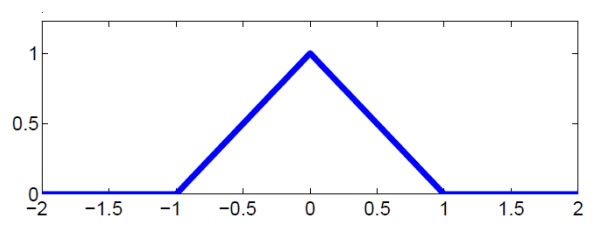
\includegraphics[width=0.5\textwidth]{MLbook/chapters/clustering/png/TSVMLoss.jpg}
    \caption{Вид функции штрафа для неразмеченных данных.}
    \end{figure}

\begin{figure}[ht]
    \centering
    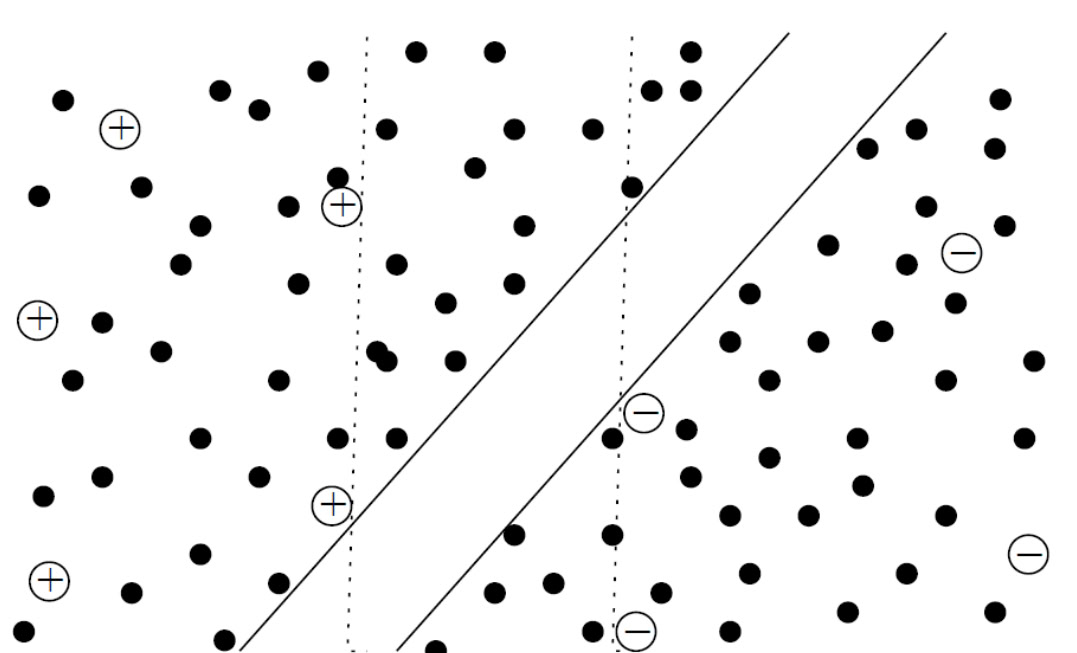
\includegraphics[width=0.5\textwidth]{MLbook/chapters/clustering/png/ClassifierData.jpg}
    \caption{Пример распределения точек около границы.}
\end{figure}

\subsection{Математическое описание трансдуктивной задачи}
С математической точки зрения новая трансдуктивная задача описывается следующим образом:

\begin{equation}
    Q(w, w_0) = \sum_{i=1}^{k} \left( 1 - \textcolor{red}{M_i(w, w_0)} \right)_+ + \frac{1}{2C} \|w\|^2 + \gamma \sum_{i=k+1}^{\ell} \left( 1 - |\textcolor{red}{M_i(w, w_0)}| \right)_+ \to \min_{\textcolor{red}{w, w_0}}.
\end{equation}

Данный подход позволяет учитывать как известные, так и неизвестные (неразмеченные) данные для более точного обучения модели.

\textbf{Основные преимущества и недостатки TSVM}:
\begin{itemize} 
    \item \textbf{Преимущества:} 
    \begin{itemize} 
        \item Как и в обычном SVM, можно использовать ядра для работы с нелинейными задачами. 
        \item Имеются эффективные реализации, которые позволяют работать с большими объемами данных. 
    \end{itemize}
        
    \item \textbf{Недостатки:}
    \begin{itemize}
        \item Задача оптимизации TSVM не является выпуклой, что делает методы оптимизации более сложными.
        \item Решение может быть неустойчивым, если нет области разреженности в данных.
        \item Требуется настройка двух параметров: \( C \) и \( \gamma \).
    \end{itemize}

    \item \textbf{Применение:} 
    TSVM используется в задачах, где важно учитывать как размеченные, так и неразмеченные данные для повышения точности классификации. Это делает метод особенно полезным для работы с большими объемами неразмеченных данных, которые часто встречаются в реальных приложениях.
\end{itemize}

\subsection{Задачи}
\subsubsection*{Номер 1}
\textbf{Условие:} Покажите на примере двух точек $(1/3, 1/3)$ и $(-2, -2)$ и линейного классификатора  с $w_0 = 0, w_1 = 1, w_2 = 1$ как именно считается модифицированная функция штрафа $L_U(M)$. \\
\textbf{Решение:}
Классифицирующей поверхностью в нашем случае является прямая $y = -x$ с соответствующей полосой, поэтому можем взять точки $(1/3, 1/3)$ и $(-2, -2)$ для того, чтобы продемонстрировать требуемое. Для них соответственно получаем:
\[
    L_1 = (1 - |(1/3*1 + 1/3*1 + 0)|)_+ = 1/3
\]

\[
    L_2 = (1 - |((-2)*1 + (-2)*1 + 0)|)_+ = 0
\]
\[
    L_{all} = 1/3 + 0 = 1/3
\]
Мы умножаем M на 1 вне зависимости от знака класса, т.к. в формуле стоит модуль, это опустили.
\subsubsection*{Номер 2}
\textbf{Условие:}
В рамках предыдущей задачи покажите, что для классификатора с теми же $w_1, w_2$, но $w_0 = -1$ получившийся штраф будет меньше. Соответствует ли это лучшей разделимости точек? Продемонстрируйте картинки с пояснениями.\\
\textbf{Решение:}
Аналогично будем иметь:
\[  
    L_1 = (1 - |(1/3*1 + 1/3*1 + 1)|)_+ = 0
\]

\[
    L_2 = (1 - |((-2)*1 + (-2)*1 + 1)|)_+ = 0
\]

\[
    L_{all} = 0 + 0 = 0
\]
Таким образом штраф уменьшился, и как видно из картинок, точки стали распределены вне линии разделения:
\begin{figure}[ht]
    \centering
    \begin{minipage}{0.45\textwidth}
        \centering
        \includegraphics[width=0.9\textwidth]{MLbook/chapters/clustering/png/TSVM_3task1.jpg}
        \caption{$w_0 = 0$}
    \end{minipage}
    \hfill
    \begin{minipage}{0.45\textwidth}
        \centering
        \includegraphics[width=0.9\textwidth]{MLbook/chapters/clustering/png/TSVM_3task2.jpg}
        \caption{$w_0 = -1$}
    \end{minipage}
\end{figure}

\subsubsection*{Номер 3}
\textbf{Условие:}
Можно ли использовать метод TSVM для постепенного самообучения, размечая данные по мере их поступления? Какие преимущества и недостатки могут быть у такого подхода?\\
\textbf{Решение:}\\
\textbf{Преимущества:}
\begin{itemize}
    \item \textbf{Эффективное использование неразмеченных данных:} Постепенное добавление размеченных данных на основе текущих предсказаний TSVM позволяет улучшить модель по мере поступления новых данных. Это может быть полезно, если размечать данные вручную дорого или занимает много времени.
    \item \textbf{Гибкость в обучении:} Метод TSVM может адаптироваться к новым данным и улучшать границу классификации, не требуя полного перерасчета модели с нуля каждый раз. Это особенно полезно в задачах, где данные поступают по мере времени (например, в потоках информации).
    \item \textbf{Обучение на малых объемах данных:} TSVM позволяет начать с небольшого набора размеченных данных и постепенно расширять его, используя информацию о неразмеченных примерах. Это важно, когда размеченные данные труднодоступны или ограничены.
\end{itemize}\\
\textbf{Недостатки:}
\begin{itemize}
    \item \textbf{Риски неправильной разметки:} Одной из проблем такого подхода является риск неверной или неточной разметки данных в процессе самообучения. Если начальная модель не обладает высокой точностью, ошибки в разметке могут привести к накоплению ошибок в дальнейшем обучении.
    \item \textbf{Проблемы с неопределенностью:} Неопределенные данные (примеры, которые находятся близко к границе принятия решения) могут быть ошибочно размечены. TSVM решает эту проблему через регуляризацию, но все же может столкнуться с трудностями при обработке сложных случаев, когда граница классификации неясна.
    \item \textbf{Зависимость от начальных данных:} Результат обучения сильно зависит от начального набора размеченных данных. Если эти данные не являются репрезентативными, то модель может в дальнейшем плохо обрабатывать новые примеры.
\end{itemize}


    \clearpage
    \chapter{Методы отбора признаков}
    \section*{Методы отбора признаков. Качество классификации.}
Рассмотрим задачу бинарной классификации с обучающей выборкой $D = \{(x_i, y_i)\}_{i=1}^n$, где $x_i \in \mathbb{R}^d$ --- вектор признаков, $y_i \in \{0, 1\}$ --- бинарная переменная.
Мы хотим построить модель $f: \mathbb{R}^d \to \{0, 1\}$, которая принимает на вход вектор признаков и выдает предсказание класса.
Есть следующие способы измерять качество модели:

Accuracy

Precision

Recall

$F_{\beta}$ score

ROC AUC

Для каждого объекта из выборки мы имеем 4 варианта разивития событий:

TP --- True Positive, классификатор предсказал 1, верное значение тоже 1

FP --- False Positive, классификатор предсказал 1, верное значение 0

TN --- True Negative, классификатор предсказал 0, верное значение тоже 0

FN --- False Negative, классификатор предсказал 0, верное значение 1


Ясно, что мы хотим видеть как можно больше TP и TN и как можно меньше FP и FN.

Accuracy --- это доля правильных ответов классификатора.
$$
    \text{Accuracy} = \frac{TP + TN}{TP + FP + TN + FN} = \frac{1}{n} \sum_{i=1}^n \mathbb{I}(y_i = f(x_i))
$$

Достаточно банальная метрика, которая не учитывает дисбаланса классов, но в качестве базового варианта подходит отлично.

Precision --- это доля объектов, которые классификатор предсказал как 1, среди всех объектов, которые он предсказал как 1.
$$
    \text{Precision} = \frac{TP}{TP + FP}
$$

Recall --- это доля объектов, которые классификатор предсказал как 1, среди всех объектов, которые действительно равны 1.
$$
    \text{Recall} = \frac{TP}{TP + FN}
$$

Precision и Recall --- базовые метрики, но по отдельности их использовать нельзя, поэтому придумали $F_{\beta}$ score.

$F_{\beta}$ score --- это взвешенное среднее гармоническое precision и recall.
$$
    F_{\beta} = (1 + \beta^2) \frac{precision \cdot recall}{\beta^2 \cdot precision + recall}
$$

$TPR$ --- это доля объектов, которые классификатор предсказал как 1, среди всех объектов, которые действительно равны 1.
$$
    TPR = \frac{TP}{TP + FN}
$$

$FPR$ --- это доля объектов, которые классификатор предсказал как 1, среди всех объектов, которые действительно равны 0.
$$
    FPR = \frac{FP}{FP + TN}
$$

Обычно, когда мы решаем задачу бинарной классификации, то мы не предсказываем явный класс, а предсказываем какое-то значение, и чем больше это значение, тем больше вероятность того, что объект принадлежит к классу 1.
Следовательно, мы можем устанавливать пороговое значение, которое будет определять, к какому классу отнести объект.
При увеличении порога отсечения мы увеличиваем количество объектов, которые отнесены к классу 0, и уменьшаем количество объектов, которые отнесены к классу 1.
Заметим, что также при увеличении порога отсечения TPR и FPR будут уменьшаться.

ROC кривая --- это кривая, которая показывает зависимость TPR от FPR при изменении порога отсечения. То есть по оси $x$ откладывается $FPR$, а по оси $y$ --- $TPR$.

Строго говоря, ROC кривая --- это множество точек вида $(FPR(t), TPR(t))$, где $t$ --- пороговое значение вероятности.

ROC-AUC --- это площадь под ROC кривой.

\subsection*{Задача 1}

Мы хотим построить модель бинарной классификации, которая будет по некоторому описанию пациента предсказывать, болен ли он раком.
В случае, если наша модель скажет, что пациент болен раком, то мы отправим его на дополнительное обследование, что обойдется пациенту в некоторую неприятную, но не критичную сумму денег.
Если же наша модель скажет, что пациент здоров, то мы ничего не будем предпринимать.
Мы хотим выбрать метрику качества для нашей модели из следующего списка: Accuracy, Precision, Recall, $F_{\beta}$ score, что нам лучше всего подойдет?
Если мы хотим выбрать $F_{\beta}$ score, то какие значения $\beta$ нам лучше всего подойдут?

\begin{solution}
Accuracy --- не лучший вариант, так как ошибка FP и FN в нашем случае не равнозначны.
Не отправить больного на дополнительное обследование значительно хуже, чем отправить здорового пациента на обследование.
Precision и Recall --- достаточно плохие метрики, ведь есть очень простая модель, которая даст 100\% Precision --- просто предсказывать, что все пациенты больны, аналогичная проблема и с Recall.
$F_{\beta}$ score --- отличный вариант, ведь с помощью $\beta$ мы можем выбирать, какое предпочтение мы отдаем Precision, а какое Recall.
В нашем случае, мы хотим, чтобы Precision был предпочтительнее Recall, поэтому $\beta$ должно быть меньше 1.
Если мы для себя решили, что смерть человека стоит как 10 дообследований, то стоит брать $\beta = \frac{1}{10}$.
\end{solution}
\subsection*{Задача 2}
Предположим, что мы измеряем качество модели с помощью ROC-AUC. Допустим, что у нас есть две модели, чьи ROC кривые выглядят следующим образом:
\begin{figure}[h]
    \centering
    \includegraphics[width=0.8\textwidth]{roc_curves_comparison_1.png}
    \caption{Две ROC кривые}
\end{figure}
Как эти модели упорядочить по качеству?

\begin{solution}
Первая модель самая худшая, ведь ее ROC кривая максимально близка к диагонали, значит она имеет миниимальную ROC-AUC.
Это плохо, но что по смыслу означает близкая к диагонали ROC кривая?

Это означает, что для любого порога отсечения $t$ имеем примерно $TPR(t) = FPR(t)$.
Что означает $TPR(t) = FPR(t)$? Это означает, что модель просто случайным образом с вероятностью $TPR(t)=FPR(t)$ предсказывает 1 класс.
Вторая модель лучшая, но почему?

А что означает график, который близок к уголку, как на рисунке 2?
Это означает, что мы можем взять такой порог отсечения $t$, что почти выполнено $TPR(t) = 1$ и $FPR(t) = 0$.
А это идеальная модель, которая никогда не ошибается.

Заметим, что чем больше площадь под ROC кривой, тем ближе эта кривая к уголку, а значит тем лучше модель.
\end{solution}
\subsection*{Задача 3}
Продолжим измерять качество моделей с помощью ROC-AUC. Допустим, что у нас есть две модели, чьи ROC кривые выглядят следующим образом:
\begin{figure}[h]
    \centering
    \includegraphics[width=0.8\textwidth]{roc_curves_comparison_2.png}
    \caption{Две ROC кривые}
\end{figure}
Как эти модели упорядочить по качеству? А как выбрать порог отсечения? В чем преимущество ROC перед $F_{\beta}$ score?

\begin{solution}
В данном случае, обе ROC кривые имеют одинаковую площадь под графиком, а значит одинаковую ROC-AUC, поэтому просто посмотреть на метрику ROC-AUC нельзя.
На самом деле, однозначного ответа нет, всё зависит от конкретной задачи.

Первая кривая быстро достигает высокого значения TPR, при не самом высоком значении FPR.

Это означает, что выбрав порог отсечения $t$, при котором $TPR(t)$ будет близок к 1, а $FPR(t)$ будет близок к 0.5, мы получим модель,
которая угадывает почти всех, кто попадает в 1 класс, но при этом не сильно много ошибается на классе 0.
Такая модель отлично подойдет в первой задаче, где мы хотим отгадать почти всех больных, но при этом не сильно много отправлять на дополнительное обследование здоровых людей.

На втором графике ситуация обратная, мы можем выбрать порог отсечения $t$, при котором $TPR(t)$ будет близок к 0.5, а $FPR(t)$ будет близок к 1.
Такая модель будет полезна в случае, когда мы хотим минимизировать количество ошибок на классе 0, но при этом не сильно много ошибаться на классе 1.
В контексте первой задачи, это означает, что мы не хотим тратить лишние деньги на дополнительное обследование здоровых людей даже ценой смерти больных, которых мы не отправляем на дополнительное обследование.

Исходя из этих примеров, становится понятно, как стоит выбирать порог отсечения. По сути его выбор означает, насколько мы готовы пожертвовать ошибками на предсказаниях одного класса, чтобы минимизировать ошибки на предсказаниях другого класса.
Это такой аналог $\beta$ в $F_{\beta}$ score, только $\beta$ мы выбирали до измерения метрики, а в случае ROC кривой мы выбираем порог отсечения глядя на график и имея какую-то дополнительную информацию о том, как работает модель при разных порогах.
Это может быть очень полезно, ведь далеко не всегда мы готовы определиться с балансом ошибок на классах перед тем, как начать решать задачу.
\end{solution}


    \clearpage
    \chapter{Логические методы классификации}
    \section{Бинаризация признаков}

Бинаризация признаков – это процесс преобразования исходных признаков в бинарные переменные, которые принимают значения \(0\) или \(1\). 
%Этот метод широко используется в задачах %машинного обучения, особенно в логических %методах классификации, где входные данные %должны быть представлены в виде набора %булевых предикатов.

\subsection{Бинаризация количественных признаков}

Для признака \( f: X \to D_f \), где \( D_f \) – множество возможных значений признака, бинаризация заключается в создании предикатов, проверяющих выполнение определённых условий. Эти предикаты позволяют разбить множество значений признака на подмножества, которые можно использовать в логических моделях.

В зависимости от типа признака, бинаризация осуществляется следующим образом:
\begin{itemize}
    \item \textbf{Номинальный признак} (\(f\) принимает конечное множество значений, без упорядоченности):
    \[
    \beta(x) = [f(x) = d], \quad d \in D_f;
    \]
    \[
    \beta(x) = [f(x) \in D'], \quad D' \subset D_f.
    \]
    \item \textbf{Порядковый или количественный признак} (\(f\) принимает значения, между которыми можно определить порядок):
    \[
    \beta(x) = [f(x) \leq d], \quad d \in D_f;
    \]
    \[
    \beta(x) = [d \leq f(x) \leq d'], \quad d, d' \in D_f, \, d < d'.
    \]
\end{itemize}

Для количественных признаков (\(f: X \to \mathbb{R}\)) важно выбирать такие пороговые значения \(d\), которые разделяют выборку на значимые группы. Например, 
%пороги \(d\) могут быть определены как средние значения между %соседними элементами вариационного ряда \(f(x_1), \dots, %f(x_\ell)\), упорядоченного по возрастанию:
\[
d_i = \frac{f^{(i)} + f^{(i+1)}}{2}, \quad f^{(i)} \neq f^{(i+1)}, \; i = 1, \dots, \ell - 1,
\]
где \(f^{(1)} \leq f^{(2)} \leq \dots \leq f^{(\ell)}\) – упорядоченные значения признака. (См. рис)

Такими способами можно получить много разных предикатов. Мы хотим выбрать из них самые ''лучшие'' (в каком-либо смысле). Для этого разобьем диапазон значений признака на зоны.

\begin{figure}
    \centering
    \includegraphics[scale = 1]{chapters/logical/images/bin1.png}
    \caption{Вариационный ряд значений признака $f(x)$ и пороги $d_i$}
\end{figure}

\subsection{Разбиение диапазона значений признака на зоны}

Каждая зона определяется бинарным предикатом:
\begin{align*}
\zeta_0(x) &= [f(x) < d_1], \\
\zeta_s(x) &= [d_s \leq f(x) < d_{s+1}], \quad s = 1, \dots, r-1, \\
\zeta_r(x) &= [d_r \leq f(x)].
\end{align*}

Способы разбиения:
\begin{itemize}
    \item Жадная максимизация информативности путем слияний
    \item Разбиение на равномощные подвыборки
    \item Разбиение по равномерной сетке ''удобных'' значений (например, с минимальным числом значащих цифр)
    \item Объединение нескольких разбиений
\end{itemize}

\subsection{Жадный алгоритм слияния зон}

Алгоритм начинает с разбиения на ''мелкие'' зоны. Пороги проходят между всеми соседними парами точек, принадлежащих \emph{разным} классам, т.~к. расстановка порогов между точками одного класса приведет только к уменьшению информативности зон. Далее зоны укрупняются путём слияния \emph{троек} соседних зон. Зоны сливаются до тех пор, пока
информативность некоторой слитой зоны превышает информативность
исходных зон, либо пока не будет получено заданное количество зон $r$. Каждый раз сливается тройка, дающая наибольший выигрыш в информативности.

\begin{figure}
    \centering
    \includegraphics[scale = 1]{chapters/logical/images/bin2.png}
    \caption{Начальное разбиение на зоны}
\end{figure}

\newpage
\textbf{Вход:}
\begin{itemize}
    \item $f(x)$ — признак;
    \item $c \in Y$ — выделенный класс;
    \item $X^\ell = \{(x_i, y_i)\}_{i=1}^\ell$ — выборка, упорядоченная по возрастанию $f(x_i)$;
    \item $r$ — желаемое количество зон;
    \item $\delta_0$ — порог слияния зон (по умолчанию $\delta_0 = 0$).
\end{itemize}

\textbf{Выход:}
\[
D = \{d_1, \dots, d_n\} \text{ — строго возрастающая последовательность порогов;}
\]

\hrule

\begin{enumerate}
    \item $D := \emptyset;$
    \item \textbf{для всех} $i = 2, \dots, \ell$:
    \begin{itemize}
        \item \textbf{если} $f(x_{i-1}) \neq f(x_i)$ и $[y_{i-1} = c] \neq [y_i = c]$ \textbf{то}
        \begin{itemize}
            \item добавить новый порог $d := \frac{f(x_{i-1}) + f(x_i)}{2}$ в конец последовательности $D$;
        \end{itemize}
    \end{itemize}
    \item \textbf{повторять}
    \begin{enumerate}
        \item \textbf{для всех} $d_i \in D, i = 1, \dots, |D| - 1$:
        \begin{itemize}
            \item вычислить выигрыш от слияния тройки соседних зон $\zeta_{i-1}, \zeta_i, \zeta_{i+1}$:
            \[
            \delta_i := I_c(\zeta_{i-1} \cup \zeta_i \cup \zeta_{i+1}) - \max\{I_c(\zeta_{i-1}), I_c(\zeta_i), I_c(\zeta_{i+1})\};
            \]
        \end{itemize}
        \item найти тройку зон, для которой слияние наиболее выгодно:
        \[
        i := \arg \max \delta_i;
        \]
        \item \textbf{если} $\delta_i > \delta_0$ \textbf{то}
        \begin{itemize}
            \item слить зоны $\zeta_{i-1}, \zeta_i, \zeta_{i+1}$, удалить пороги $d_i$ и $d_{i+1}$ из последовательности $D$;
        \end{itemize}
    \end{enumerate}
    \item \textbf{пока} $|D| > r + 1$.
\end{enumerate}

\subsection{Задачи}

\textbf{Задача 1}
Предположим, вы владелец интернет-магазина, и у вас есть данные о стоимости товаров и их популярности (популярен — \( 1 \), непопулярен — \( 0 \)). 
Для анализа спроса вы хотите разбить товары на ценовые зоны, чтобы лучше понять поведение покупателей.

Данные представлены в таблице:

\[
\begin{array}{|c|c|c|}
\hline
\text{№ товара} & \text{Цена товара (\$)} & \text{Популярность } y \\
\hline
1 & 10 & 1 \\
2 & 12 & 1 \\
3 & 15 & 0 \\
4 & 17 & 1 \\
5 & 20 & 0 \\
6 & 23 & 0 \\
7 & 25 & 1 \\
\hline
\end{array}
\]

Как алгоритм слияния зон первично разобьёт выборку на ценовые зоны?

\textbf{Решение}
Рассчитаем пороги:

\[
\begin{aligned}
&d_1 = \frac{12 + 15}{2} = 13.5, \\
&d_2 = \frac{15 + 17}{2} = 16.0, \\
&d_3 = \frac{17 + 20}{2} = 18.5, \\
&d_4 = \frac{23 + 25}{2} = 24.0
\end{aligned}
\]

На основе рассчитанных порогов получаем зоны:

\[
\begin{aligned}
&\zeta_0(x) = [\text{Цена} < 13.5], \\
&\zeta_1(x) = [13.5 \leq \text{Цена} < 16.0], \\
&\zeta_2(x) = [16.0 \leq \text{Цена} < 18.5], \\
&\zeta_4(x) = [29.0 \leq \text{Цена} < 24.0], \\
&\zeta_5(x) = [\text{Цена} \geq 24.0].
\end{aligned}
\]

\textbf{Задача 2}
Будут ли разбиения диапазона меняться в зависимости от класса, относительно которого они производятся? Как изменить алгоритм для получения ''универсального'' разбиения, учитывающего сразу все классы? 

\textbf{Решение}
Да, будут, т.~к. информативность зависит от класса. Нужно заменить критерий информативности многоклассовым критерием.

\textbf{Задача 3}
Какую сложность имеет алгоритм слияния зон? Как можно его ускорить?

\textbf{Решение}
Этот алгоритм имеет трудоёмкость $O(l^2)$. Его можно заметно ускорить, если на каждой итерации сливать не одну тройку зон, а $\tau l$ троек с достаточно большим выигрышем $\delta I_i$, при условии, что они не перекрываются. В этом случае трудоёмкость составляет $O(l / \sqrt{\tau})$.






\section{Разновидности решающих списков}

Логику решающего списка или, что то же самое, комитета старшинства, имеют многие алгоритмы, предлагавшиеся в разное время разными авторами под разными названиями. Многочисленные варианты отличаются выбором семейств предикатов $\Phi$, критерием информативности и методом поиска информативных предикатов.

\textbf{Пример} Наиболее распространены решающие списки конъюнкций. Они почти идеально соответствуют человеческой логике принятия решений, основанной на последовательной проверке достаточности простых правил. Поэтому решающие списки часто используются для представления знаний, извлекаемых непосредственно из эмпирических данных. Для построения отдельных правил можно использовать жадный алгоритм построения решающего списка, применяя любой из методов поиска информативных конъюнкций, например, «градиентный» алгоритм синтеза конъюнкции, либо алгоритм ТЭМП с параметром $T_0 = 1$.

\textbf{Пример} Жадный алгоритм построения решающего списка с семейством предикатов параметрического семейства шаров $\Phi$ строит покрытие обучающей выборки шарами (data dependent balls). Очень похожий алгоритм описан Маршандом и др. под названием BuildSCM. Решающие списки шаров хорошо работают, когда метрика $\rho(x, x')$ удовлетворяет гипотезе компактности, т. е. близкие объекты часто оказываются в одном классе. Если это не так, то будет построено слишком большое количество шаров небольшого радиуса. Такие алгоритмы обладают невысокой обобщающей способностью.

\textbf{Пример} Алгоритм дробящихся эталонов ДРЭТ также основан на покрытии выборки шарами, и отличается тем, что список строится от конца к началу. На первом шаге для каждого из классов определяется минимального радиуса, включающий все обучающие объекты данного класса. Если шары разных классов
пересекаются, то для объектов, попавших в пересечение, снова строятся покрывающие шары, но уже меньшего радиуса. Процесс построения шаров продолжается, пока в пересечениях шаров остаются представители разных классов. Построенные шары образуют решающий список в порядке возрастания их радиусов.

\begin{figure}[h!] \centering \includegraphics{MLbook/chapters/logical/images/logical.png} \caption{Построение решающего списка из трёх полуплоскостей.} \end{figure}

Непосредственное применение жадного алгоритма построения решающего списка к семейству предикатов семейства полуплоскостей позволяет построить покрытие обучающей выборки полуплоскостями. В этом случае решающий список описывает кусочно-линейную разделяющую поверхность между классами.

Известно большое количество эвристик для последовательного построения разделяющих полуплоскостей.

\textbf{Пример} Алгоритм Белледго строит полуплоскости, отделяющие как можно больше объектов одного класса, что равносильно максимизации информативности предиката, относящихся к параметрическому семейству полуплоскостей. Для этого применяются методы линейного программирования. В отличие от жадного алгоритма, после построения каждой полуплоскости делается попытка найти лучшие положения предыдущих полуплоскостей.

\textbf{Пример} В алгоритме Маршанда и др. перебираются всевозможные гиперплоскости, разделяющие какие-нибудь три точки (data dependent half-spaces), и из них выбирается полуплоскость с максимальной информативностью.

\subsection*{Достоинства решающих списков.}

\begin{itemize} \item Интерпретируемость и простота классификации. Обученное по выборке правило классификации можно записать в виде инструкции и выполнять «вручную». \item Гибкость: в зависимости от выбора множества $\Phi$ можно строить весьма разнообразные алгоритмические конструкции. \item Возможность обработки разнородных данных и данных с пропусками. \end{itemize}

\subsection*{Недостатки решающих списков.}

\begin{itemize} \item Если множество правил $\Phi$ выбрано неудачно, список может не построиться. При этом возможен высокий процент отказов от классификации. \item Возможна утрата интерпретируемости, если список длинный и правила различных классов следуют вперемежку. В этом случае правила не могут быть интерпретированы по-отдельности, без учёта предшествующих правил, и логика их взаимодействия становится довольно запутанной. \item Каждый объект классифицируется только одним правилом, что не позволяет правилам компенсировать неточности друг друга. Данный недостаток устраняется путём голосования правил, но это уже совсем другой алгоритм. \end{itemize}

\subsection*{Задачи}

\textbf{Задача 1.} Рассмотрим задачу построения решающего списка с использованием покрывающих шаров. Пусть у нас есть два класса $A$ и $B$ и множество объектов с координатами на плоскости:
A={(0,0),(1,0),(2,0)},B={(3,3),(4,3)}.
A={(0,0),(1,0),(2,0)},B={(3,3),(4,3)}.

Необходимо построить последовательность покрывающих шаров, начиная с класса $A$, так чтобы каждый последующий шар покрывал все объекты данного класса, но не пересекался с уже выделенными объектами другого класса. Найдите:

    Минимальный радиус шара, покрывающего все объекты класса $A$.

    Если этот шар пересекает хотя бы один объект класса $B$, постройте следующий шар для класса $B$ с наименьшим радиусом, покрывающим все оставшиеся объекты класса $B$.

\textbf{Решение 1.}
Минимальный шар, покрывающий точки $(0,0), (1,0), (2,0)$, будет иметь центр в точке $(1,0)$ и радиус $R_A = 1$. Он покрывает точки $(0,0)$ и $(2,0)$ за счёт расположения на прямой оси $x$. Поскольку объекты класса $B$ лежат далеко (в районе $(3,3)$ и $(4,3)$), они не входят в этот шар. Значит, нет пересечения с классом $B$ и можно зафиксировать первый шар радиусом $R_A = 1$. Далее для класса $B$ минимальный шар, покрывающий точки $(3,3)$ и $(4,3)$, будет иметь центр в точке $(3.5, 3)$ и радиус $R_B = 0.5$. В итоге получаем решающий список из двух шаров: первый для класса $A$ радиуса 1, второй для класса $B$ радиуса 0.5.

\medskip

\textbf{Задача 2.} Рассмотрим задачу построения решающего списка с использованием полуплоскостей. Пусть у нас есть выборка точек на плоскости:
A={(1,1),(2,1),(1,2)},B={(3,1),(3,2)}.
A={(1,1),(2,1),(1,2)},B={(3,1),(3,2)}.

Требуется найти полуплоскость, максимально отделяющую класс $A$ от $B$. То есть найдите такую линейную неравенство вида $w_1 x + w_2 y + b \geq 0$, что в одной полуплоскости окажется как можно больше точек класса $A$ и как можно меньше точек класса $B$.

\textbf{Решение 2.}
Опишем подход. Пусть мы хотим максимизировать число объектов класса $A$ в положительной полуплоскости и минимизировать число объектов класса $B$ в ней. Для решения подобной задачи можно сформулировать задачу линейного программирования: ввести индикаторные переменные, отвечающие за правильное отделение точек, и попытаться максимизировать суммарный «вес» классифицированных точек класса $A$ при ограничениях, не допускающих попадания многих точек класса $B$ в ту же полуплоскость. Геометрически для данного набора можно проверить несколько направлений: например, если взять прямую, проходящую между точками $(2,1)$ и $(3,1)$, под наклоном с положительным коэффициентом наклона, то удаётся поместить все точки $A$ в полуплоскость слева, а точки $B$ справа. Например, неравенство вида $x + y - 3 \geq 0$ поместит $(1,1)$ и $(1,2)$ в отрицательную полуплоскость (так как $1+1-3=-1<0$ и $1+2-3=0$ на границе), а $(2,1)$ в отрицательную ($2+1-3=0$ на границе). Выбирая чуть иное смещение, например $x + y - 2.5 \geq 0$, можно добиться того, чтобы все $A$ оказались по одну сторону, а $B$ — по другую. Таким образом, последовательно подбирая коэффициенты, добиваемся «лучшего» разделения классов.

\medskip

\textbf{Задача 3.} Рассмотрим решающий список из $N$ правил, где каждая строка — это предикат $\varphi_t(x)$ и соответствующий класс $c_t$. Предположим, что каждая проверка предиката занимает время $O(1)$, но интерпретация списка человеком усложняется пропорционально $N$. Пусть $N = 10$ — список довольно понятен, $N = 100$ — список уже трудно интерпретировать, а при $N = 1000$ практически невозможно понять логику классификации. Предположим, что каждая новая добавляемая строка увеличивает точность на 1%, но при этом на 10 единиц усложняет интерпретацию (условная метрическая оценка сложности).

    Определите, насколько уменьшится интерпретируемость при увеличении числа правил с $N = 10$ до $N = 1000$.

    При каком $N$ целесообразно остановиться с точки зрения баланса между точностью (+1% за правило) и интерпретируемостью (каждое правило добавляет 10 условных единиц сложности)?

\textbf{Решение 3.}
Если при $N=10$ сложность условно равна $10 \cdot 10 = 100$ единиц, то при $N=1000$ сложность будет $1000 \cdot 10 = 10000$ единиц. Интерпретируемость, обратно пропорциональная сложности, значительно упадёт, примерно в 100 раз, если считать, что интерпретируемость обратно пропорциональна числу правил.

    Если каждое правило добавляет 1\% к точности, то при увеличении с $10$ до $1000$ правил мы повысим точность на $990\%$, что не имеет смысла (точность не может превышать 100\%). Но если представить, что начальная точность была, скажем, 60\%, то до 100\% нам нужно всего 40 правил. Значит, достижение 100\% точности произойдёт уже при $N=50$. Проверим сложность: при $N=50$ сложность будет $50 \cdot 10 = 500$ единиц, что в 5 раз больше начального варианта с $N=10$. Это может быть приемлемым компромиссом. Таким образом, если нам не нужно «абсолютное» повышение точности, есть смысл остановиться при числе правил $N$, при котором точность уже удовлетворительна (например, близка к 100\%), а сложность ещё не стала слишком высокой.






\section{Взвешенное голосование правил}

Допустим, имеется консилиум экспертов, каждый член которого может допустить ошибку. Процедура голосования — это способ повышения качества принимаемых решений, при котором ошибки отдельных экспертов компенсируют друг друга.

Ранее принцип голосования применялся для построения композиций из произвольных алгоритмов классификации. Теперь рассмотрим композиции, состоящие из логических закономерностей.

\subsection{Принцип голосования}

Пусть для каждого класса $c \in Y$ построено множество логических закономерностей (правил), специализирующихся на различении объектов данного класса:

\[
R_c = \{ \varphi_{tc} : X \to \{0, 1\} \mid t = 1, \dots, T_c \}
\]

Считается, что если $\varphi_{tc}(x) = 1$, то правило $\varphi_{tc}$ относит объект $x \in X$ к классу $c$. Если же $\varphi_{tc}(x) = 0$, то правило воздерживается от классификации объекта $x$.

Алгоритм простого голосования (simple voting) подсчитывает долю правил в наборах $R_c$, относящих объект $x$ к каждому из классов:

\[
\Gamma_c(x) = \frac{1}{T_c} \sum_{t=1}^{T_c} \varphi_{tc}(x), \quad c \in Y,
\]

и относит объект $x$ к тому классу, за который подана наибольшая доля голосов:

\[
a(x) = \arg \max_{c \in Y} \Gamma_c(x).
\]

Если максимум достигается одновременно на нескольких классах, выбирается тот, для которого цена ошибки меньше.

Нормирующий множитель $\frac{1}{T_c}$ вводится для того, чтобы наборы с большим числом правил не перетягивали объекты в свой класс.

\subsection{Алгоритм взвешенного голосования}
Алгоритм взвешенного голосования (weighted voting, WV) действует более тонко, учитывая, что правила могут иметь различную ценность. Каждому правилу $\varphi_{tc}$ приписывается вес $\alpha_{tc} \geq 0$, и при голосовании берется взвешенная сумма голосов:

\[
\Gamma_c(x) = \sum_{t=1}^{T_c} \alpha_{tc} \varphi_{tc}(x), \quad \alpha_{tc} > 0.
\]

Веса нормируются на единицу:

\[
\sum_{t=1}^{T_c} \alpha_{tc} = 1, \quad \forall c \in Y.
\]

Поэтому функцию $\Gamma_c(x)$ называют также выпуклой комбинацией правил $\varphi_1, \dots, \varphi_{T_c}$. Очевидно, простое голосование является частным случаем взвешенного, когда веса одинаковы и равны $\frac{1}{T_c}$.

На первый взгляд, вес правила должен определяться его информативностью. Однако, важно также учитывать, насколько данное правило уникально. Если имеется 10 хороших, но одинаковых (или почти одинаковых) правил, их суммарный вес должен быть сравним с весом столь же хорошего правила, не похожего на все остальные. Таким образом, веса должны учитывать не только ценность правил, но и их различность.

Простой общий подход к настройке весов заключается в том, чтобы сначала найти набор правил $\{ \varphi_{tc}(x) \}$, затем принять их за новые (бинарные) признаки и построить в этом новом признаковом пространстве линейную разделяющую поверхность (кусочно-линейную, если $|Y| > 2$). Для этого можно использовать логистическую регрессию, однослойный персептрон или метод опорных векторов. Существуют и другие подходы. Например, в разделе 1.5.4 будет рассмотрен метод бустинга, в котором правила настраиваются последовательно, и для каждого правила сразу вычисляется его вес.

\subsection{Проблема диверсификации правил}
Голосующие правила должны быть существенно различны, иначе они будут бесполезны для классификации. Продолжая аналогию с консилиумом, заметим, что нет никакого смысла держать в консилиуме эксперта A, если он регулярно подсматривает решения у эксперта B.

Приведем простое теоретико-вероятностное обоснование принципа диверсификации, или повышения различности (diversity) правил \cite{14}. Пусть $X$ — вероятностное пространство, множество ответов $Y$ конечно. Введем случайную величину $M(x)$, равную перевесу голосов в пользу правильного класса; её называют также отступом (margin) объекта $x$ от границы классов:

\[
M(x) = \Gamma_c(x) - \Gamma_{\overline{c}}(x), \quad \Gamma_{\overline{c}}(x) = \max_{y \in Y \setminus \{c\}} \Gamma_y(x), \quad c = y^*(x).
\]

Если отступ положителен ($M(x) > 0$), то алгоритм голосования правильно классифицирует объект $x$. Предположим, что в среднем наш алгоритм классифицирует хотя бы немного лучше, чем наугад: $E[M] > 0$. Тогда можно оценить вероятность ошибки по неравенству Чебышева:

\[
P\{M < 0\} \leq P\{|E[M] - M| > E[M]\} \leq \frac{D_M}{(E[M])^2}.
\]

Отсюда вывод: для уменьшения вероятности ошибки необходимо максимизировать ожидание перевеса голосов $E[M]$ и минимизировать его дисперсию $D_M$. Для выполнения этих условий каждый объект должен выделяться примерно одинаковым числом правил. Обычно ни одно из правил не выделяет класс целиком, поэтому правила должны быть существенно различны, то есть выделять существенно различные подмножества объектов.

Неплохая эвристика, усиливающая различия между правилами и позволяющая равномернее выделять объекты обучения, используется в алгоритме CORAL \cite{12}. Сначала для фиксированного класса $c \in Y$ строится покрывающий набор правил точно так, как это делалось для решающих списков. Затем строится второй покрывающий набор, но при этом запрещается использовать признаки, часто входившие в закономерности первого набора. Поэтому второй набор неминуемо окажется отличным от первого. Затем запрещаются признаки, часто входившие в оба набора, и строится третий набор. И так далее, для каждого класса $c \in Y$.

\subsection{Отказы от классификации}
Возможны ситуации, когда ни одно из правил не выделяет классифицируемый объект $x$. Тогда алгоритм должен либо отказываться от классификации, либо относить объект к классу, имеющему наименьшую цену ошибки. Отказ алгоритма означает, что данный объект является нетипичным, не подпадающим ни под одну из ранее обнаруженных закономерностей. Вообще, обнаружение нетипичности (novelty detection) принято считать отдельным видом задач обучения по прецедентам, наряду с классификацией и кластеризацией. Способность алгоритмов отказываться от классификации нетипичных объектов во многих приложениях является скорее преимуществом, чем недостатком. В то же время, число отказов не должно быть слишком большим.

Итак, при построении алгоритмов взвешенного голосования правил возникает четыре основных вопроса:
\begin{itemize}
    \item Как построить много правил по одной и той же выборке?
    \item Как избежать повторов и построения почти одинаковых правил?
    \item Как избежать появления непокрытых объектов и обеспечить равномерное покрытие всей выборки правилами?
    \item Как определять веса правил при взвешенном голосовании?
\end{itemize}

Рассмотрим, как эти проблемы решаются в известных алгоритмах в следующих параграфах.

\subsection{Задачи}

\textbf{Задача 1: Алгоритм простого голосования}

Допустим, для класса $c \in Y$ существуют 10 правил, которые используют данные для классификации. Каждое правило возвращает 1 или 0 для объекта $x$. Если для объекта $x$ правила 3 и 7 верно классифицируют объект как класс $c$, а остальные возвращают 0, как будет рассчитана доля голосов для класса $c$?

\textbf{Решение:}  
Для класса $c$ доля голосов рассчитывается как сумма всех правил, которые классифицируют объект как класс $c$, делённая на общее количество правил. Если 10 правил, то:
\[
\Gamma_c(x) = \frac{1}{10} \left( 1 + 0 + 0 + 0 + 0 + 0 + 1 + 0 + 0 + 0 \right) = \frac{2}{10} = 0.2
\]
Таким образом, для объекта $x$ доля голосов для класса $c$ составит 0.2.

\textbf{Задача 2: Проблема с весами в алгоритме взвешенного голосования}

В алгоритме взвешенного голосования веса для каждого правила нормируются на единицу. Если для класса $c$ у нас есть 3 правила с весами $\alpha_1 = 0.5$, $\alpha_2 = 0.3$, и $\alpha_3 = 0.2$, как будет выглядеть итоговая сумма голосов $\Gamma_c(x)$, если объект $x$ классифицируется всеми тремя правилами как класс $c$?

\textbf{Решение:}  
Итоговая сумма голосов для класса $c$ рассчитывается по формуле:
\[
\Gamma_c(x) = \sum_{t=1}^{T_c} \alpha_{tc} \varphi_{tc}(x)
\]
где $\varphi_{tc}(x) = 1$, если правило классифицирует объект как класс $c$, и 0 в противном случае. Если все 3 правила классифицируют объект как $c$, то:
\[
\Gamma_c(x) = 0.5 + 0.3 + 0.2 = 1.0
\]

\textbf{Задача 3: Проблема диверсификации правил}

Какова вероятность ошибки при использовании алгоритма голосования, если все правила сильно похожи друг на друга (например, классифицируют одинаковые подмножества объектов)?

\textbf{Решение:}  
Если правила сильно похожи, то вероятность ошибки возрастает. В таких случаях, возможно, правило не будет существенно различать объекты, и алгоритм может ошибаться при классификации новых объектов. Чтобы уменьшить вероятность ошибки, правила должны быть разнообразными, то есть они должны выделять разные подмножества объектов. Для максимизации различий между правилами можно использовать метод, как в алгоритме CORAL, который строит покрывающие наборы правил, постепенно исключая часто встречающиеся признаки.

\textbf{Задача 4: Принцип диверсификации правил}

Пусть для объекта $x$ имеется 10 правил, из которых 8 классифицируют объект как класс $c$, а остальные 2 — как класс $d$. Какой отступ $M(x)$ будет при расчете вероятности правильной классификации?

\textbf{Решение:}  
Отступ для объекта $x$ определяется как разница между голосами для правильного класса и максимальным голосом для всех остальных классов:
\[
M(x) = \Gamma_c(x) - \Gamma_{\overline{c}}(x)
\]
Если из 10 правил 8 голосуют за класс $c$ (доля голосов $0.8$) и 2 — за класс $d$ (доля голосов $0.2$), то:
\[
M(x) = 0.8 - 0.2 = 0.6
\]
Если отступ положителен ($M(x) > 0$), то классификация будет правильной.

\textbf{Задача 5: Отказы от классификации}

Если для объекта $x$ не существует правила, которое его классифицирует, что должен делать алгоритм голосования? Как можно обработать такой случай?

\textbf{Решение:}  
В таком случае алгоритм может либо отказаться от классификации, либо отнести объект к классу с наименьшей ценой ошибки. Такой отказ от классификации часто называют обнаружением нетипичности (novelty detection), что является отдельной задачей в машинном обучении. Важно, чтобы количество отказов не было слишком большим, так как это может снизить эффективность алгоритма.

\section{Решающие списки}
\subsection{Опреление}
    Решающий список - это логический алгоритм классификации $a: X \xrightarrow{} Y$, задаваемый закономерностями $\varphi_1, \dots, \varphi_T$ классов $c_1, \dots, c_T \in Y$, вычисляемый следующим алоритмом

\hline
\begin{enumerate}
    \item \textbf{для всех} $t = 1, \dots, T_{max}$:
    \begin{itemize}
        \item \textbf{если} $\varphi_t(x) = 1$ 
        \begin{itemize}
            \item \textbf{вернуть $c_t$}
        \end{itemize}
    \end{itemize}
    
    \item \textbf{вернуть $c_0$}
\end{enumerate}
\hline
«Особый ответ» $c_0$ означает отказ алгоритма от классификации объекта $x$.
Обычно такие объекты приписывают классу, имеющему минимальную цену ошибки.
Например, в задаче выдачи кредитов отказ алгоритма приведёт к более осторожному решению «не выдавать». В задаче распознавания спама более осторожным будет
решение «не спам».

\textbf{Замечание} Соседние правила в списке $\varphi_{t-1}, \varphi_t$ можно переставлять местами,
если только они приписаны к одному классу, $c_{t-1} = c_t$. В общем случае перестановка
правил в списке изменяет алгоритм.

\subsection{Жадный алгоритм посторения}
Рассмотрим жадный алгоритм построения решающих списков.

Алгоритм, приведённый ниже, на каждой итерации строит ровно одно правило $\varphi_t$, выделяющее максимальное число объектов некоторого класса $c_t$ и минимальное число объектов
всех остальных классов. Для этого на каждой итерации производится поиск наиболее информативного правила $\varphi_t \in \Phi$, допускающего относительно мало ошибок. Семейство
правил $\Phi$ может быть каким угодно, лишь бы для него существовала эффективная
процедура поиска закономерностей. После построения правила $\varphi_t$ выделенные им объекты изымаются из выборки и алгоритм переходит к поиску следующего правила $\varphi_{t+1}$ по оставшимся объектам. В итоге выборка оказывается покрытой
множествами вида $\{x: \varphi_t(x) = 1\}$. Поэтому решающий список называют также покрывающим набором закономерностей или машиной покрывающих множеств.

\hline
\textbf{Вход:}
\begin{itemize}
    \item $X^l$ -- выборка;
    \item $T_{max}$ -- максимальное допустимое число правил в списке;
    \item $I_{min}$ -- минимальная допустимая информативность правил в списке;
    \item $E_{max}$ -- максимальная допустимая доля ошибок на обучающей выборке;
    \item $l_0$ -- максимальное допустимое число отказов.
\end{itemize}

\textbf{Выход:}
 $\{\varphi_1, \dots, \varphi_T\} \text{ — искомые решающие правила;}$

\hline
\begin{enumerate}
    \item $U := X^l;$
    \item \textbf{для всех} $i = 1, \dots, T_{max}$:
    \begin{itemize}
        \item \text{вычираем класс} $c := c_t$
        \item найти наиболее информативное правило при ограничении на долю ошибок:\
        $\varphi_t := \arg\min_{\varphi \in \Phi'} I_c(\varphi, U)$, где $\Phi' = \{ \varphi \in \Phi \ | \ E_c(\varphi, U) \leq E_{max} \}$ 

        \item \textbf{если} $I_c(\varphi_t, U) \leq I_{min}$ \textbf{то выход}
        \item Исключить из выборки объекты, выделенные правилом $\varphi_t$:
        $U := \{x \in U | \varphi_t(x) = 0\}$

        \item \textbf{если} $|U| \leq l_0$ \textbf{то выход}
    \end{itemize}
\end{enumerate}
\hline

\subsection{Анализ алгоритма}

\textbf{Критерии отбора правил.} Почему приходится использовать сразу два критерия
отбора правил $I_c$ и $E_c$? Правило с высокой информативностью $I_c$ вполне может допускать значительную долю ошибок $E_c$. Это нежелательно, так как в решающем списке каждое правило принимает окончательное решение. С другой стороны, правило с небольшой долей ошибок может выделять слишком мало объектов,
и по этой причине не являться закономерностью. Совместное использование обоих
критериев позволяет отобрать предикаты, удовлетворяющие условиям как статистической, так и логической закономерности.

\textbf{Критерии останова.} В данном алгоритме одновременно работают три критерия останова: 

(1) построение заданного числа правил $T_{max}$; 

(2) покрытие всей выборки, за исключением не более $l_0$ объектов; 

(3) невозможность найти правило с информативностью выше Imin по остатку выборки.

\textbf{Оптимизация сложности решающего списка.} Параметр $E_{max}$ позволяет найти
компромисс между точностью классификации обучающего материала и сложностью
списка. Уменьшение $E_{max}$ приводит к снижению числа ошибок на обучении. С другой
стороны, оно ужесточает отбор правил, способствует уменьшению числа объектов,
выделяемых отдельными правилами, и увеличению длины списка $T$. Правила, выделяющие слишком мало объектов, статистически не надёжны и могут допускать много
ошибок на независимых контрольных данных. Иными словами, увеличение длины
списка при одновременном «измельчении» правил может приводить к эффекту переобучения. Из общих соображений Emax должно быть приблизительно равно доле
ошибок, которую мы ожидаем получить как на обучающей выборке, так и вне её.
На практике параметр Emax подбирается экспериментально.

\textbf{Стратегия выбора класса.} Мы ничего не сказали о том, как выбирается класс $c_t$. Рассмотрим два варианта.
Первый вариант — сначала строятся все правила для первого класса, затем для второго, и так далее. Классы берутся в порядке убывания важности или цены ошибки. Преимущество данного варианта в том, что правила оказываются независимыми — в пределах своего класса их можно переставлять местами. Это улучшает
интерпретируемость правил.
Второй вариант — совместить 2 шага и выбирать пару $(\varphi_t
, c_t) \in \Phi \times Y$ , для
которой информативность $I_{c_t}(\varphi_t, U)$ максимальна. Тогда правила различных классов
могут следовать вперемежку. Доказано, что списки такого типа реализуют более широкое множество функций. При этом улучшается разделяющая способность
списка, но ухудшается его интерпретируемость.
На практике первый вариант часто оказывается более удобным. В некоторых случаях правила строятся только для $(M − 1)$ классов, а в последний, наименее
важный, класс $c_0$ объекты заносятся «по остаточному принципу».
Обработка пропусков в данных. Решающие списки позволяют легко обойти проблему пропущенных данных. Если для вычисления предиката 
$\varphi_t(x)$ не хватает данных, то считается, что $\varphi_t(x) = 0$, и обработку объекта $x$ берут на себя следующие
правила в списке. Это относится и к стадии обучения, и к стадии классификации.

\subsection{Разновидности решающих списков}
Логику решающего списка или, что то же самое, комитета старшинства, имеют
многие алгоритмы, предлагавшиеся в разное время разными авторами под разными названиями. Многочисленные варианты отличаются выбором семейства предикатов $\Phi$, критерием информативности и методом поиска информативных предикатов.

\textbf{Пример} Наиболее распространены решающие списки конъюнкций. Они почти
идеально соответствуют человеческой логике принятия решений, основанной на последовательной проверке достаточно простых правил. Поэтому решающие списки
часто используются для представления знаний, извлекаемых непосредственно из эмпирических данных. Для построения отдельных правил можно использовать жадный алгоритм, применяя для поиска $\varphi$ любой из методов поиска информативных конъюнкций,
например.

\textbf{Пример} В алгоритме Маршанда перебираются всевозможные гиперплоскости, разделяющие какие-нибудь три точки (data dependent half-spaces), и из них выбирается полуплоскость с максимальной информативностью.

\subsection{Достоинства и недостатки}

\textbf{Достоинства решающих списков.}
\begin{enumerate}
    \item Интерпретируемость и простота классификации. Обученное по выборке правило классификации можно записать в виде инструкции и выполнять «вручную».
    \item Гибкость: в зависимости от выбора множества $\Phi$ можно строить весьма разнообразные алгоритмические конструкции.
    \item Возможность обработки разнотипных данных и данных с пропусками.
\end{enumerate}
\\
\textbf{Недостатки решающих списков.}
\begin{enumerate}
    \item Если множество правил $\Phi$ выбрано неудачно, список может не построиться. При этом возможен высокий процент отказов от классификации.
    \item Возможна утрата интерпретируемости, если список длинный и правила различных классов следуют вперемежку. В этом случае правила не могут быть
    интерпретированы по-отдельности, без учёта предшествующих правил, и логика их взаимодействия становится довольно запутанной.
    \item Каждый объект классифицируется только одним правилом, что не позволяет
    правилам компенсировать неточности друг друга. Данный недостаток устраняется путём голосования правил, но это уже совсем другой алгоритм.
\end{enumerate}

\subsection{Задачи}

\textbf{Задача 1}
Постройте решающий список для логической функции $x \vee y \vee \overline{z}.$

\textbf{Решение}

\includegraphics[scale = 0.5]{images/decide_list_task1_sol.png}

\textbf{Задача 2}
Адаптируйте решающий список для задач регрессии.

\textbf{Решение}
Давайте разобъём множество значений искомой зависимости $y: X \rightarrow{} Y$ на $T + 1$ множеств вида:
$[y < d_1], [d_1 \leq y < d_2], ..., [d_{T-1} \leq y < d_T], [d_T \leq y].$ 
Сопоставим эти множества с классами $c_1, \dots, c_T$.

Теперь запустим алгоритм построения решающего списка для полученных классов, 
но помимо нахождения правил $\varphi$, будем так же находить среднее значение $y$ на объектах, которые удовлетворяют этому правилу.
И будем выдавать по объекту $x$ среднее значение для объектов этого класса.

\section {Решающие таблицы}
\subsection{Опреление}

Решающая таблица - это частный стлучай решающего дерева глубины $H$, для всех узлов уровня $h$ условия ветвления $f_h(x)$ одинаковы. На уровне $h$ ровно $2^{h-1}$ вернин. $X$ делится на $2^H$ "ячеек".

\textbf{Пример.} Задача XOR, $H = 2$.

    \includegraphics[scale = 0.5]{images/decide_table_exapmle.png}

\subsection{Жадный алгоритм посторения}
Рассмотрим жадный алгоритм построения решающей таблицы

\hline
\textbf{Вход:}
\begin{itemize}
    \item $X^l$ — выборка;
    \item $F$ - множество признаков ;
    \item $H$ - глубина дерева.
\end{itemize}

\textbf{Выход:}
\begin{itemize}
    \item $\{f_1, \dots, f_H\};$ 
    \item таблица $T: \{0, 1\}^H \xrightarrow{} Y$
\end{itemize}

\hline
\begin{enumerate}
    \item $U := X^l;$
    \item \textbf{для всех} $h = 1, \dots, H$:
    \begin{itemize}
        \item предикат с максимальным выигрышем определённости:
        $f_h := \arg\min_{f \in F} Gain(f_1, \dots, f_{h-1}, f)$
    \end{itemize}
    \item классификация по мажоритарному правилу 
    $ T(\beta) := Major(U_{H\beta}) $
\end{enumerate}
\hline
Выигрыш от ветвления на уровне $h$ по всей выборке $X^L$:
$$Gain(f_1, \dots, f_h) = \Phi(X^l) - \sum_{\beta\in \{0, 1\}^h} \frac{U_{h\beta}}{l}\Phi(U_{h\beta})$$

$U_{h\beta} = \{ x_i \in X^l \ | \ f_s(x_i)=\beta_s,\ s=1\dots h \}, \beta=(\beta_1, \dots, \beta_h) \in \{0, 1\}^h$

$p_y =\frac{1}{|U|} \sum_{x_i \ in U}[y_i = y]$ -- частичная оценка $P(y|U)$.

$\Phi(U)$ -- мера неопределённости распределения $p_y$:
\begin{enumerate}
    \item минимальная  равна нулю, когда $p_y \in \{0,1\}$
    \item ксимальна, когда $p_y = \frac{1}{|Y|}$ -- номерное распределение
    \item симметрична, то есть не зависи от перенумерации классов
\end{enumerate}

\subsection{Задачи}

\textbf{Задача}
Постройте решающую таблицу для логической функции $x \vee (y \wedge \overline{z}).$ Изобразите её ввиде дерева.

\textbf{Решение}
\begin{figure}
    \centering
    \includegraphics[width=0.5\linewidth]{decide_table_task_sol.png}
\end{figure}

\section{Алгоритм КОРА}

Алгоритм комбинаторного распознавания КОРА, предложенный М.М.~Бонгардом в 1961 году и реализованный М.Н.~Вайнцвайгом, предназначен для построения набора конъюнктивных закономерностей. Этот алгоритм неоднократно демонстрировал высокую эффективность при решении различных прикладных задач, связанных с распознаванием образов и классификацией.

\subsection{Основные эвристические предположения}

Для эффективной работы алгоритма КОРА сделаны следующие эвристические предположения:

\begin{itemize}
    \item \textbf{Адекватность множества предикатов:} Множество элементарных предикатов \(B\) выбрано таким образом, что среди конъюнкций ранга 2 или 3 уже содержится достаточное количество информативных закономерностей.
    \item \textbf{Ограничение ранга конъюнкций:} Поскольку ранг конъюнкций ограничен числом 3, для поиска закономерностей возможно применение полного перебора, что упрощает процесс поиска.
    \item \textbf{Непротиворечивость закономерностей:} Наибольший интерес представляют те закономерности, которые являются непротиворечивыми, то есть не содержат противоречий в данных.
\end{itemize}

\subsection{Пример дерева перебора}

На рисунке \ref{fig:kora_tree} показано дерево полного перебора конъюнкций в алгоритме КОРА при \(|B| = 4\). Для краткости конъюнкции обозначены номерами составляющих их предикатов.

\begin{figure}[h]
    \centering
    \includegraphics[width=0.6\textwidth]{images/kora_tree.png}
    \caption{Дерево полного перебора конъюнкций в алгоритме КОРА при \(|B| = 4\). Для краткости конъюнкции обозначены номерами составляющих их предикатов.}
    \label{fig:kora_tree}
\end{figure}

\subsection{Описание алгоритма}

Алгоритм КОРА строит конъюнкции, состоящие не более чем из \(K\) термов, выбранных из множества предикатов \(B\). Основой алгоритма является рекурсивная процедура \textit{Нарастить}(\(\varphi\)), которая добавляет термы в конъюнкцию \(\varphi(x)\) всевозможными способами. При этом в список закономерностей \(R_c\) заносятся только наиболее информативные конъюнкции.

\subsubsection{Параметры алгоритма}

Алгоритм использует следующие параметры:

\begin{itemize}
    \item \(D_{\text{min}}\) — минимальная доля позитивных объектов для конъюнкций.
    \item \(E_{\text{max}}\) — максимальная допустимая доля ошибок.
    \item \(T_{\text{min}}, T_{\text{max}}\) — ограничения на количество конъюнкций в списке.
\end{itemize}

\subsubsection{Построение списка информативных конъюнкций методом поиска в глубину (алгоритм КОРА)}

\textbf{Входные данные:}
\begin{itemize}
    \item \(X_\ell\) — обучающая выборка;
    \item \(B\) — семейство элементарных предикатов;
    \item \(K\) — максимальный ранг конъюнкций;
    \item \(E_{\text{max}}\) — максимальная доля ошибок \(E_c(\varphi)\) для конъюнкций \(\varphi \in R_c\);
    \item \(D_{\text{min}}\) — минимальная доля позитивных объектов \(D_c(\varphi)\) для конъюнкций \(\varphi \in R_c\);
    \item \(T_{\text{min}}, T_{\text{max}}\) — ограничения на количество конъюнкций \(T_c\).
\end{itemize}

\textbf{Выходные данные:} 
Списки конъюнкций \(R_c = \{ \varphi_{tc}(x) : t = 1, \dots, T_c \}, \) для всех \(c \in Y\).

\begin{enumerate}
    \item Инициализировать списки: \(R_c = \emptyset\) для всех \(c \in Y\).
    \item Повторять:
    \begin{itemize}
        \item Выполнить \textit{Нарастить}(\(\emptyset\));
        \item Определить \(T := \min_{c \in Y} |R_c|\);
        \item Если \(T < T_{\text{min}}\), то уменьшить \(D_{\text{min}}\) и/или увеличить \(E_{\text{max}}\);
        \item Если \(T > T_{\text{max}}\) или время поиска становится слишком большим, то увеличить \(D_{\text{min}}\) и/или уменьшить \(E_{\text{max}}\);
    \end{itemize}
    \item Пока \(T \notin [T_{\text{min}}, T_{\text{max}})\).
\end{enumerate}

\subsubsection{Процедура \textit{Нарастить}(\(\varphi\))}

\begin{enumerate}
    \item Если \(\varphi = \emptyset\), установить \(j_s := 0\).
    \item Для всех \(j \in \{ j_s + 1, \dots, |B| \}\):
    \begin{itemize}
        \item Добавить терм \(\beta_j\) к исходной конъюнкции:
        \[
        \varphi' := \varphi \wedge \beta_j
        \]
        \item Если \(|\varphi'| \leq K\) и существует \(c \in Y\), такое что:
        \[
        D_c(\varphi') > D_{\text{min}} \quad \text{и} \quad E_c(\varphi') \leq E_{\text{max}},
        \]
        то добавить \(\varphi'\) в список \(R_c\).
        \item Иначе, если \(|\varphi'| < K\) и существует \(c \in Y\), такое что \(D_c(\varphi') > D_{\text{min}}\), то рекурсивно вызвать \textit{Нарастить}(\(\varphi'\)).
    \end{itemize}
\end{enumerate}

\subsubsection{Включение конъюнкции \(\varphi\) в список \(R_c\), содержащий не менее \(T\) самых информативных конъюнкций}

Этот алгоритм предназначен для поддержания в списке \(R_c\) не менее \(T\) самых информативных конъюнкций. Эта процедура обеспечивает управление количеством конъюнкций в списке и поддержание их порядка по информативности.

\begin{enumerate}
    \item \textbf{Процедура} \textit{Добавить\_в\_список}( \(R_c\), \(\varphi\), \(T\) ):
    \item Вставить конъюнкцию \(\varphi\) в список \(R_c\) в порядке убывания информативности \(I_c(\varphi)\).
    \item Найти наименьшую информативность в списке:
    \[
    J := \min_{\psi \in R_c} I_c(\psi)
    \]
    \item Определить количество конъюнкций с наименьшей информативностью:
    \[
    \Delta := \#\{ \psi \in R_c : I_c(\psi) = J \}
    \]
    \item Если \(|R_c| - \Delta > T\), то удалить из списка \(R_c\) все конъюнкции с информативностью \(J\).
\end{enumerate}

\subsection{Достоинства алгоритма КОРА}

\begin{itemize}
    \item \textbf{Интерпретируемость:} Короткие конъюнкции легко интерпретируются в терминах предметной области.
    \item \textbf{Эффективность:} При малых значениях \(K\) (например, \(K \leq 3\)) алгоритм работает очень эффективно.
    \item \textbf{Полнота:} Если существуют короткие информативные конъюнкции, алгоритм обязательно их найдет.
\end{itemize}

\subsection{Недостатки алгоритма КОРА}

\begin{itemize}
    \item \textbf{Зависимость от предикатов:} При неудачном выборе множества предикатов \(B\) короткие информативные конъюнкции могут отсутствовать.
    \item \textbf{Экспоненциальная сложность:} Увеличение числа \(K\) приводит к экспоненциальному росту вычислительной сложности.
    \item \textbf{Отсутствие диверсификации:} Алгоритм не стремится диверсифицировать конъюнкции и обеспечивать равномерное покрытие объектов.
\end{itemize}

\section{Алгоритм ТЭМП}

Полный перебор всех конъюнкций ранга не более $K$ требует экспоненциального по $K$ числа операций. В реальных задачах объём вычислений становится огромным уже при $K > 3$, и от идеи полного перебора приходится отказаться.

Существует две стандартные стратегии перебора конъюнкций: поиск в глубину (depth-first search) и поиск в ширину (breadth-first search). Первая применяется в алгоритме КОРА, вторая — в алгоритме ТЭМП, предложенным Г. С. Лбовым в 1976 году. Поиск в ширину работает немного быстрее, и в него легче встраивать различные эвристики, сокращающие перебор.

В исходном варианте алгоритм ТЭМП выполнял полный перебор всех конъюнкций ранга не более $K$. Ниже описан слегка модифицированный вариант, позволяющий ограничить перебор и увеличить максимальный ранг конъюнкций $K$.

Алгоритм 1.9 начинает процесс поиска закономерностей с построения конъюнкций ранга 1. Для этого отбираются не более $T_1$ самых информативных предикатов из базового множества $\mathcal{B}$. Затем к каждому из отобранных предикатов добавляется по одному терму из $\mathcal{B}$ всеми возможными способами. Получается не более $T_1|\mathcal{B}|$ конъюнкций ранга 2, из которых снова отбираются $T_1$ самых информативных. И так далее. На каждом шаге процесса делается попытка добавить один терм к каждой из имеющихся конъюнкций. Наращивание конъюнкций прекращается либо при достижении максимального ранга $K$, либо когда ни одну из конъюнкций не удаётся улучшить путём добавления терма.

Лучшие конъюнкции, собранные со всех шагов, заносятся в списки $R_c$. Таким образом, списки $R_c$ могут содержать конъюнкции различного ранга.

Параметр $T_1$ позволяет найти компромисс между качеством и скоростью работы алгоритма. При $T_1 = 1$ алгоритм ТЭМП работает исключительно быстро и строит единственную конъюнкцию, добавляя термы по очереди. Фактически, он совпадает с жадным Алгоритмом 1.2. При увеличении $T_1$ пространство поиска расширяется, алгоритм начинает работать медленнее, но находит больше информативных конъюнкций. На практике выбирают максимальное значение параметра $T_1$, при котором поиск занимает приемлемое время. Однако стратегия поиска всё равно остаётся жадной — термы оптимизируются по-отдельности, и при подборе каждого терма учитываются только предыдущие, но не последующие термы.

Для улучшения конъюнкций к ним применяют эвристические методы «финальной шлифовки» — стабилизацию и редукцию.

В результате стабилизации конъюнкции становятся локально неулучшаемыми. Алгоритм в целом становится более устойчивым — при незначительных изменениях в составе обучающей выборки он чаще находит одни и те же закономерности, а значит, улучшается его способность обобщать эмпирические факты.

В результате стабилизации некоторые конъюнкции могут совпасть, и в списке появятся дубликаты. Их удаление предусмотрено на шаге 13. Если список $R_c$ поддерживается отсортированным по информативности, то удаление дубликатов является недорогой операцией, так как достаточно проверять на совпадение только соседние конъюнкции с одинаковой информативностью.

Если задать $T_1 = \infty$, то алгоритм выполнит полный перебор, как в исходном варианте ТЭМП. «Финальная шлифовка» в этом случае не нужна.

\subsection{Алгоритм 1.9. Построение списка информативных конъюнкций методом поиска в ширину (алгоритм ТЭМП)}


\subsection{Алгоритм 1.9: Построение списка информативных конъюнкций методом поиска в ширину}

\textbf{Вход:}
\begin{itemize}
    \item $X_\ell$ --- обучающая выборка;
    \item $\mathcal{B}$ --- семейство элементарных предикатов;
    \item $c \in Y$ --- класс, для которого строится список конъюнкций;
    \item $K$ --- максимальный ранг конъюнкций;
    \item $T_1$ --- число лучших конъюнкций, отбираемых на каждом шаге;
    \item $T_0$ --- число лучших конъюнкций, отбираемых на последнем шаге, $T_0 \leq T_1$;
    \item $I_{\min}$ --- порог информативности;
    \item $E_{\max}$ --- порог допустимой доли ошибок;
    \item $X_k$ --- контрольная выборка для проведения редукции.
\end{itemize}

\textbf{Выход:} Список конъюнкций $R_c = \{\varphi_t^c(x) : t = 1, \dots, T_c\}$.

\begin{enumerate}
    \item $R_c \gets \emptyset$;
    \item Для всех $\beta \in \mathcal{B}$: \texttt{Добавить\_в\_список($R_c$, $\beta$, $T_1$)};
    \item Для всех $k = 2, \dots, K$:
    \begin{enumerate}
        \item Для всех конъюнкций $\varphi \in R_c$ ранга $(k-1)$:
        \begin{enumerate}
            \item Для всех предикатов $\beta \in \mathcal{B}$, которых ещё нет в конъюнкции $\varphi$:
            \begin{enumerate}
                \item Добавить терм $\beta$ к конъюнкции $\varphi$: $\varphi' = \varphi \land \beta$;
                \item Если $I_c(\varphi') > I_{\min}$, $E_c(\varphi') \leq E_{\max}$ и конъюнкции $\varphi'$ нет в $R_c$, то \texttt{Добавить\_в\_список($R_c$, $\varphi'$, $T_1$)}.
            \end{enumerate}
        \end{enumerate}
    \end{enumerate}
    \item Для всех конъюнкций $\varphi \in R_c$:
    \begin{enumerate}
        \item Стабилизация($\varphi$);
        \item Редукция($\varphi$, $X^k$);
    \end{enumerate}
    \item Удалить из списка $R_c$ дублирующие конъюнкции;
    \item Оставить в списке $R_c$ не более $T_0$ лучших конъюнкций.
\end{enumerate}


\subsection{Достоинства алгоритма ТЭМП}

\begin{itemize}
    \item ТЭМП существенно более эффективен, чем КОРА, особенно при поиске конъюнкций ранга больше 3. Он решает поставленную задачу за $O(KT_1|B|\\ell)$ операций, тогда как КОРА имеет трудоёмкость $O(|B|K\\ell)$.
    \item Параметр $T_1$ позволяет управлять жадностью алгоритма и находить компромисс между качеством конъюнкций и скоростью работы алгоритма.
    \item Благодаря простоте и эффективности алгоритм ТЭМП можно использовать в составе других алгоритмов как генератор конъюнкций, достаточно близких к оптимальным.
\end{itemize}

\subsection{Недостатки алгоритма ТЭМП}

\begin{itemize}
    \item Нет гарантии, что будут найдены самые лучшие конъюнкции, особенно при малых значениях параметра $T_1$.
    \item Алгоритм не стремится увеличивать различность конъюнкций, добиваясь равномерного покрытия объектов выборки. Стабилизация и редукция лишь отчасти компенсируют этот недостаток.
    \item Нет настройки коэффициентов $\\alpha_{tc}$; предполагается простое голосование.

\end{itemize}

\subsection{Задачи}

\textbf{Задача 1}  
Рассмотрим множество элементарных предикатов \( B = \{ \beta_1, \beta_2, \beta_3 \} \) и обучающую выборку \( X_\ell \) с классами \( Y = \{A, B\} \). Предположим, что следующие конъюнкции удовлетворяют условиям \( D_{\text{min}} \) и \( E_{\text{max}} \):

\[
\varphi_1 = \beta_1 \wedge \beta_2, \quad \varphi_2 = \beta_2 \wedge \beta_3, \quad \varphi_3 = \beta_1 \wedge \beta_3
\]

Определите, какие из этих конъюнкций будут добавлены в списки \( R_A \) и \( R_B \) после выполнения процедуры \textit{Нарастить}(\(\emptyset\)).

\textbf{Решение}  
Процедура \textit{Нарастить} начинает с пустой конъюнкции и добавляет термы по одному. Проверяем каждую конъюнкцию на удовлетворение условий \( D_{\text{min}} \) и \( E_{\text{max}} \):

\begin{itemize}
    \item \(\varphi_1 = \beta_1 \wedge \beta_2\): Если для класса \(A\) \(D_A(\varphi_1) > D_{\text{min}}\) и \(E_A(\varphi_1) \leq E_{\text{max}}\), то \(\varphi_1\) добавляется в \( R_A \). Аналогично проверяется для класса \(B\).
    \item \(\varphi_2 = \beta_2 \wedge \beta_3\): Аналогично, добавляется в соответствующие списки классов.
    \item \(\varphi_3 = \beta_1 \wedge \beta_3\): Аналогично, добавляется в соответствующие списки классов.
\end{itemize}

Таким образом, все три конъюнкции будут добавлены в списки \( R_A \) и \( R_B \), если они удовлетворяют заданным условиям.

\textbf{Задача 2}  
Предположим, что при использовании алгоритма КОРА параметр \( K \) увеличен с 3 до 4. Объясните, как это повлияет на эффективность алгоритма и количество генерируемых конъюнкций.

\textbf{Решение}  
Увеличение параметра \( K \) с 3 до 4 расширяет максимальный ранг конъюнкций, позволяя создавать более сложные правила с дополнительным термом. Однако это приводит к экспоненциальному росту числа возможных конъюнкций, что значительно снижает эффективность алгоритма из-за увеличения вычислительной сложности. Кроме того, при большем \( K \) может возрастать вероятность переобучения, так как алгоритм будет генерировать больше конъюнкций, что может привести к снижению обобщающей способности модели.

\textbf{Задача 3}  
Рассмотрим ситуацию, когда множество предикатов \( B \) плохо выбрано, и среди конъюнкций ранга 2 или 3 отсутствуют информативные закономерности. Как это повлияет на работу алгоритма КОРА и какие меры можно предпринять для улучшения результатов?

\textbf{Решение}  
Если множество предикатов \( B \) плохо выбрано и среди конъюнкций ранга 2 или 3 отсутствуют информативные закономерности, алгоритм КОРА не сможет эффективно выявить необходимые закономерности, что приведет к низкой точности классификации. Для улучшения результатов можно предпринять следующие меры:

\begin{enumerate}
    \item \textbf{Пересмотр множества предикатов \( B \):} Добавить новые предикаты или изменить существующие, чтобы повысить их информативность.
    \item \textbf{Увеличение максимального ранга \( K \):} Хотя это снижает эффективность, иногда требуется более высокий ранг для захвата сложных закономерностей.
    \item \textbf{Использование методов отбора признаков:} Применить методы отбора признаков для выбора наиболее информативных предикатов, что может улучшить качество конъюнкций.
    \item \textbf{Комбинирование с другими алгоритмами:} Интегрировать КОРА с другими алгоритмами машинного обучения для улучшения общего качества модели.
\end{enumerate}

Эти меры помогут повысить информативность конъюнкций и, соответственно, эффективность алгоритма КОРА.

\textbf{Задача 1.}
\newline
Рассмотрите граф $G = (V, E)$, где $V = \{A, B, C, D, E\}$ и $E = \{(A, B), (A, C), (B, D), (C, D), (D, E)\}$. Как алгоритм ТЭМП выполняет поиск в ширину для этого графа? Предложите, как можно выполнить поиск в глубину.

\textit{Решение:}
\begin{enumerate}
    \item Алгоритм ТЭМП начинает с вершины $A$, добавляя её соседей $B$ и $C$ в очередь. Затем из очереди выбирается вершина $B$, её сосед $D$ добавляется в очередь, и так далее.
    \item Для поиска в глубину из вершины $A$ алгоритм выбирает один путь (например, $A \to B \to D \to E$), пока не дойдёт до конца, затем возвращается и ищет другие пути.
\end{enumerate}

\textbf{Задача 2.}
\newline
Пусть у нас есть множество предикатов $B = \beta_1, \beta_2, \beta_3$ и максимальный ранг $K = 2$. Какое количество конъюнкций будет проверено алгоритмом ТЭМП, если для каждого шага выбирается $T_1 = 2$? Если мы увеличим $T_1$ до 3, как это повлияет на количество проверяемых конъюнкций?

\textit{Решение:}
\begin{itemize}
    \item При $T_1 = 2$ для ранга 1 будет 2 конъюнкции, для ранга 2 --- $2 \times 3 = 6$ конъюнкций. Всего будет проверено $2 + 6 = 8$ конъюнкций.
    \item Если $T_1 = 3$, то для ранга 1 будет 3 конъюнкции, для ранга 2 --- $3 \times 3 = 9$ конъюнкций. Всего будет проверено $3 + 9 = 12$ конъюнкций.
\end{itemize}

\textbf{Задача 3.}
\newline
Представьте, что вы используете алгоритм ТЭМП для обучения модели с большим количеством предикатов. Какой будет влияние на время вычислений, если вы увеличите $T_1$ с 1 до 5? Объясните это с точки зрения расширения пространства поиска.

\textit{Решение:}
\begin{itemize}
    \item При $T_1 = 1$ алгоритм будет проверять только по одному терму для каждой конъюнкции на каждом шаге, что будет довольно быстрым, но может не давать лучшие результаты.
    \item При увеличении $T_1$ до 5 пространство поиска расширяется, так как на каждом шаге будет добавляться больше термов к конъюнкциям, что увеличивает количество проверяемых комбинаций и тем самым замедляет процесс.
    \item В результате увеличение $T_1$ может существенно замедлить алгоритм, но при этом улучшится качество найденных решений.
\end{itemize}


\section{Решающие деревья регрессии.}

Деревья регрессии - тип деревьев решений. Он используется в случае, когда целевой признак является непрерывным, например, действительным числом. Дерево имеет два типа вершин:
\begin{itemize}
    \item Внутренние вершины, переходы из которых осуществляются при помощи применения предикатов к признакам объекта.
    \item Листья, содержащие предсказания целевого признака. При этом значения для листьев вычисляются на этапе обучения как функция от значений целевого признака для всех объектов тренировочной выборки, попадающих в эту вершину. В отличие от классифицирующего дерева, здесь получается конкретное значение, а не класс и не вектор вероятностей принадлежности к классам.
\end{itemize}
Таким образом, регрессионные решающие деревья позволяют получать приближения целевой функции при помощи кусочно-постоянных функций.

\subsection{Построение регрессионных решающих деревьев}
Для построения регрессионных деревьев используется алгоритм CART (Classification And Regression Trees). Сначала нужно выбрать критерий разбиения, то есть меру неопределенности, которую мы будем минимизировать при поиске наилучшего способа разбить вершину.

\subsubsection{Метрики построения}
В случае регрессионных решающих деревьев используются метрики, подходящие для непрерывных значений целевого признака. Среди них наиболее популярны MSE и MAE:
\begin{itemize}
    \item  Средняя квадратичная ошибка (MSE): Измеряет среднюю квадратичную разницу между наблюдаемыми и предсказанными значениями на тренировочной выборке:
    \begin{align*}
        MSE = \frac{1}{n} \sum_{i=1}^{n} (y_i - \hat{y}_i)^2
    \end{align*} 
    \item Средняя абсолютная ошибка (MAE): Измеряет среднюю абсолютную разницу между наблюдаемыми и прогнозируемыми значениями на тренировочной выборке.
    \begin{align*}
        MAE = \frac{1}{n} \sum_{i=1}^{n} |y_i - \hat{y}_i|
    \end{align*}
\end{itemize}

Зачастую для избежания переобучения к минимизируемой функции также добавляется штраф, связанный с числом вершин в дереве.

\subsubsection{Процесс построения}
После выбора метрики осуществляется жадное рекурсивное построение дерева. На каждом шаге выбирается вершина, и задача заключается в выборе такого предиката, который бы разбивал множество приходящих в неё объектов обучающей выборки наилучшим с точки зрения минимизации метрики ошибки способом. Для этого перебираются все признаки, и для каждого признака подбирается оптимальное пороговое значение, после чего выбирается признак, дающий наилучший результат. В случае, если ни одно из разбиений не даёт подходящего результата, вершина остаётся листом. Также разбиение может прекратиться в случае, если установлено ограничение на количество вершин.

Для рекурсивного выполнения алгоритма процесс запускается из корневой вершины, после чего при каждом разбиении последующей вершины запускается также для её дочерних вершин.

\subsubsection{Усечение ветвей}

Решающие деревья склонны к переобучению из-за того, что с увеличением глубины каждую вершину достигает всё меньшее число объектов. Для решения этой проблемы используется усечение ветвей (pruning). Идея заключается в проверке работы дерева на данных, не использовавшихся при обучении, и отбрасывании поддеревьев с большой ошибкой. Чтобы применить этот метод, нужно изначально выделить часть обучающей выборки, которая будет использоваться только при прунинге.

Различают два подхода к усечению ветвей: обход дерева от корня к листьям и от листьев к корню.     

\begin{itemize}
    \item Top-down pruning — подход, при котором проверка и обрезка наименее информативных ветвей начинается с корневого узла. Данный метод обладает относительно низкой вычислительной сложностью, однако может приводить к недообучению за счёт удаления ветвей, которые могли потенциально содержать информативные узлы. В качестве примера можно привести Pessimistic Error Pruning (PEP). При таком подходе удаляются поддеревья с наибольшей ошибкой на отложенной выборке, порог устанавливается заранее.
    
    \item Bottom-up pruning — подход, при котором проверка и обрезка наименее информативных ветвей начинается с листьев. В данном случае получаются более точные деревья за счёт оценки каждого узла по отдельности. Но из-за полного обхода дерева увеличивается вычислительная сложность. Среди методов данного подхода можно выделить следующие:
    \begin{itemize}
        \item Reduced Error Pruning (REP), когда решающие узлы удаляются до тех пор, пока не падает точность, измеренная на отложенной выборке;

        \item Cost-complexity pruning (CCP), когда последовательно строится серия поддеревьев исходного дерева через удаление слабейших узлов. После этого наилучшее дерево можно выбрать при проверке на тестовой выборке.
    \end{itemize}
\end{itemize}

При усечении поддерева можно использовать один из следующих вариантов:
\begin{itemize}
    \item Оставить поддерево без изменений,
    \item Заменить поддерево одним из дочерних,
    \item Объединить дочерние поддеревья и заново рассчитать предсказание.
\end{itemize}
Выбор происходит с точки зрения минимизации меры неопределенности.

\subsection{Преимущества и недостатки регрессионных решающих деревьев}

В качестве преимуществ решающих деревьев регрессии стоит выделить:
\begin{itemize}
    \item Интерпретируемость. Последовательный анализ признаков с учетом результатов применения предыдущих предикатов схож с процессом мышления человека.
    \item Алгоритмическая сложность использования. Количество операций пропорционально глубине дерева, а сравнение -- быстрая операция, что позволяет неглубоким деревьям работать быстро.
    \item Определение наиболее важных признаков. В процессе построения разбиение начинается с признаков, дающих наибольшую информацию об объекте, и решающие деревья хорошо справляются с ситуацией, когда часть признаков информативнее других.
    \item Приближение нелинейных зависимостей. Кусочно-линейные функции позволяют сколь угодно хорошо приблизить большое количество функций и не требуют предварительного анализа характера зависимости.
\end{itemize}

Недостатки регрессионных решающих деревьев:
\begin{itemize}
    \item Сложность построения. В общем случае для поиска оптимального дерева необходимо перебирать все возможные варианты деревьев, что является np-полной задачей.
    \item Чувствительность к выбросам. Поскольку деревья решений разбивают выборку на подмножества исходя из минимизации значения метрики, они могут выделять выбросы с сильно отличающимися от остальных значениями, что значительно уменьшает штраф. В таком случае для объектов, находящиеся вблизи выброса, будут сделаны неверные предсказания. 
    \item Переобучение. Из-за того, что к глубоким вершинам относятся всё меньшие по мощности подмножества обучающей выборки, дерево может переобучиться под конкретные элементы. Для этого приходится проводить пост-обработку, устанавливать ограничение на число вершин, или включать дополнительные штрафы в минимизируемую функцию.
\end{itemize}

\subsection{Задачи для закрепления материала}
\textbf{Задача 1} (Использование регрессионных решающих деревьев)

    Дано решающее дерево, возвращающее значение целевого признака $y$ из $Y = \mathbb{R}$ для объектов с признаками $x_1$ и $x_2$ из $X = [0, 1] \times \mathbb{R}$:
    \begin{itemize}
        \item Если $x_2 \geq 0$:
        \begin{itemize}
            \item Если $x_1 > 0.25$, то $y = 0$,
            \item Иначе $y = 1$
        \end{itemize}
        \item Иначе:
        \begin{itemize}
            \item Если $x_1 > 0.5$:
            \begin{itemize}
                \item Если $x_2 < -100$, то $y = -100$,
                \item Иначе $y = -5$.
            \end{itemize}
            \item Иначе, $y = -1$.
        \end{itemize}
    \end{itemize}

    Найдите предсказание для объекта $x = (0.75, -1)$.

    \textbf{Решение.}
    Начнем спускаться из корня дерева, проверяя условия для нашего $x$.
    \begin{enumerate}
        \item Условие в корне: $x_2 \geq 0$. Оно неверно для нашего $x$, идем во вторую ветвь.
        \item Условие в следующей вершине: $x_1 > 0.5$. Оно верно для нашего $x$, поэтому идем в первую ветвь.
        \item Условие в следующей вершине: $x_2 < -100$. Оно неверно для нашего $x$, поэтому выбираем вторую ветвь и получаем значение $y = -5$.
    \end{enumerate}

    Таким образом, предсказание для нашего объекта: $y = -5$.
    
    
\textbf{Задача 2} (Построение регрессионного решающего дерева)
    
    Дана тренировочная выборка из 6 объектов, $X = [0, 6]$, $Y = \mathbb{R}$. Необходимо построить регрессионное решающее дерево при помощи алгоритма CART с метрикой MSE.
    \begin{table}[h]
    \centering
    \caption{Выборка.}
    \begin{tabular}{|c|c|c|c|c|c|c|}
    \hline
    $x$ & $1$ & $2$ & $3$ & $4$ & $5$ & $6$ \\
    \hline
    $y$ & $2$ & $0$ & $6$ & $8$ & $10$ & $12$ \\
    \hline
    \end{tabular}
    \end{table}

    \textbf{Решение.}
    У нас есть всего один нецелевой признак, поэтому все предикаты будут относиться к нему. В качестве метрики выберем $MSE$. В таком случае оптимальное значение для листа будет средним арифметическим значений целевого признака всех объектов тренировочной выборки, попадающих в эту вершину.

    Начнем с корневой вершины. Среднее арифметическое целевого признака для всех объектов сейчас равно $6.3$, значение метрики $107.3$. Изобразим это на графике \ref{regression_trees::plot0}. 
    
    \begin{center}
    \begin{tikzpicture}[scale = 1.5] \label{regression_trees::plot0}
    % Draw the axes
    \draw[->] (0,0) -- (6.5,0) node[right] {$x$};
    \draw[->] (0,0) -- (0,3.5) node[above] {$y$};

    % Draw points
    \foreach \Point in {(1,0.5), (2,0), (3,1.5), (4,2), (5,2.5), (6,3)}{
        \node at \Point {\textbullet};
    }

    % Draw the piecewise linear function
    \draw[red, thick] (0,38/24) -- (6,38/24);

    % Draw grid lines for better visualization (optional)
    \foreach \x in {0,0.5,1,1.5,2,2.5,3,3.5,4,4.5,5,5.5,6}
        \draw[gray, dashed] (\x,0) -- (\x,3.5);
    \foreach \y in {0,0.25,0.5,0.75,1,1.25,1.5,1.75,2,2.25,2.5,2.75,3,3.25}
        \draw[gray, dashed] (0,\y) -- (6,\y);

    % Axis labels
    \foreach \x in {0,1,2,3,4,5,6}
        \node at (\x,-0.25) {\x};
    \foreach \x in {2,4,6,8,10,12}
        \node at (-0.25,0.25*\x) {\x};

    \end{tikzpicture}
    \end{center}
    
    Вычислим значение метрики для всех возможных разделений объектов на два множества по пороговому значению $x$ в таблице \ref{regression_trees::table1}.
    \begin{table}[h] 
    \centering
    \caption{Вычисление метрики для различных способов разбиения.}
    \begin{tabular}{|c|c|c|c|c|c|}
    \hline
    Диапазон порогового значения & $(1, 2)$ & $(2, 3)$ & $(3, 4)$ & $(4, 5)$ & $(5, 6)$ \\
    \hline
    Пред. для объектов с $x$ меньше порога & $2$ & $1$ & $2.7$ & $4$ & $5.2$ \\
    \hline
    Пред. для объектов с $x$ больше порога & $7.2$ & $9$ & $10$ & $11$ & $12$ \\
    \hline
    MSE для дерева & $84.8$ & $22$ & $26.7$ & $42$ & $68.8$ \\
    \hline
    \end{tabular} \label{regression_trees::table1}
    \end{table}
    
    Таким образом, оптимальное разбиение лежит в диапазоне между $2$ и $3$. Возьмем среднее $2.5$, поскольку это позволит относить объекты к тому подмножеству, которому оно ближе. Изобразим на графике \ref{regression_trees::plot1} новую функцию, задаваемую деревом.
    
    \begin{center}
    \begin{tikzpicture}[scale = 1.5] 
    % Draw the axes
    \draw[->] (0,0) -- (6.5,0) node[right] {$x$};
    \draw[->] (0,0) -- (0,3.5) node[above] {$y$};

    % Draw points
    \foreach \Point in {(1,0.5), (2,0), (3,1.5), (4,2), (5,2.5), (6,3)}{
        \node at \Point {\textbullet};
    }

    % Draw the piecewise linear function
    \draw[red, thick] (0,0.25) -- (2.5,0.25);
    \draw[red, thick] (2.5,0.25) -- (2.5,2.25);
    \draw[red, thick] (2.5,2.25) -- (6,2.25);

    % Draw grid lines for better visualization (optional)
    \foreach \x in {0,0.5,1,1.5,2,2.5,3,3.5,4,4.5,5,5.5,6}
        \draw[gray, dashed] (\x,0) -- (\x,3.5);
    \foreach \y in {0,0.25,0.5,0.75,1,1.25,1.5,1.75,2,2.25,2.5,2.75,3,3.25}
        \draw[gray, dashed] (0,\y) -- (6,\y);

    % Axis labels
    \foreach \x in {0,1,2,3,4,5,6}
        \node at (\x,-0.25) {\x};
    \foreach \x in {2,4,6,8,10,12}
        \node at (-0.25,0.25*\x) {\x};

    \end{tikzpicture}
    \label{regression_trees::plot1}
    \end{center}

    Проведем разветвление для подмножества с большими значениями $x$. Исходное значение MSE для поддерева равно $20$. Вычислим его для всех вариантов разбиения в таблице \ref{regression_trees::table2}.
    \begin{table}[h] 
    \centering
    \caption{Вычисление метрики для различных способов разбиения.}
    \begin{tabular}{|c|c|c|c|} 
    \hline
    Диапазон порогового значения & $(3, 4)$ & $(4, 5)$ & $(5, 6)$ \\
    \hline
    Пред. для объектов с $x$ меньше порога & $6$ & $7$ & $8$ \\
    \hline
    Пред. для объектов с $x$ больше порога & $10$ & $11$ & $12$ \\
    \hline
    MSE для дерева & $8$ & $4$ & $8$ \\
    \hline
    \end{tabular}
    \label{regression_trees::table2}
    \end{table}

    Таким образом, эффективнее поставить границу между $4$ и $5$, аналогично возьмем среднее $4.5$.

    Оба разбиения достаточно хороши и превосходят результат для поддерева без разбиения ($8$). Выберем первое из них, положив границу $4.5$. Новый график - \ref{regression_trees::plot2}. Левым поддеревом будем называть то поддерево, которое работает с множеством левее по оси $x$.

    \begin{center}
    \begin{tikzpicture}[scale = 1.5] \label{regression_trees::plot2}
    % Draw the axes
    \draw[->] (0,0) -- (6.5,0) node[right] {$x$};
    \draw[->] (0,0) -- (0,3.5) node[above] {$y$};

    % Draw points
    \foreach \Point in {(1,0.5), (2,0), (3,1.5), (4,2), (5,2.5), (6,3)}{
        \node at \Point {\textbullet};
    }

    % Draw the piecewise linear function
    \draw[red, thick] (0,0.25) -- (2.5,0.25);
    \draw[red, thick] (2.5,0.25) -- (2.5,1.75);
    \draw[red, thick] (2.5,1.75) -- (4.5,1.75);
    \draw[red, thick] (4.5,1.75) -- (4.5,2.75);
    \draw[red, thick] (4.5,2.75) -- (6,2.75);

    % Draw grid lines for better visualization (optional)
    \foreach \x in {0,0.5,1,1.5,2,2.5,3,3.5,4,4.5,5,5.5,6}
        \draw[gray, dashed] (\x,0) -- (\x,3.5);
    \foreach \y in {0,0.25,0.5,0.75,1,1.25,1.5,1.75,2,2.25,2.5,2.75,3,3.25}
        \draw[gray, dashed] (0,\y) -- (6,\y);

    % Axis labels
    \foreach \x in {0,1,2,3,4,5,6}
        \node at (\x,-0.25) {\x};
    \foreach \x in {2,4,6,8,10,12}
        \node at (-0.25,0.25*\x) {\x};

    \end{tikzpicture}
    \end{center}

    Далее можно провести разбиение трех получившихся множеств, разделяя их посередине между значениями $x$, и присваивая листьям значения $y$ соответствующих $x$. Это уменьшит значение MSE всего дерева до нуля. Изобразим итоговую функцию на графике \ref{regression_trees::plot3}.

    \begin{center}
    \begin{tikzpicture}[scale = 1.5] \label{regression_trees::plot3}
    % Draw the axes
    \draw[->] (0,0) -- (6.5,0) node[right] {$x$};
    \draw[->] (0,0) -- (0,3.5) node[above] {$y$};

    % Draw points
    \foreach \Point in {(1,0.5), (2,0), (3,1.5), (4,2), (5,2.5), (6,3)}{
        \node at \Point {\textbullet};
    }

    % Draw the piecewise linear function
    \draw[red, thick] (0,0.5) -- (1.5,0.5);
    \draw[red, thick] (1.5,0) -- (2.5,0);
    \draw[red, thick] (2.5,1.5) -- (3.5,1.5);
    \draw[red, thick] (3.5,2) -- (4.5,2);
    \draw[red, thick] (4.5,2.5) -- (5.5,2.5);
    \draw[red, thick] (5.5,3) -- (6,3);
    
    \draw[red, thick] (1.5,0) -- (1.5,0.5);
    \draw[red, thick] (2.5,0) -- (2.5,1.5);
    \draw[red, thick] (3.5,1.5) -- (3.5,2);
    \draw[red, thick] (4.5,2) -- (4.5,2.5);
    \draw[red, thick] (5.5,2.5) -- (5.5,3);

    % Draw grid lines for better visualization (optional)
    \foreach \x in {0,0.5,1,1.5,2,2.5,3,3.5,4,4.5,5,5.5,6}
        \draw[gray, dashed] (\x,0) -- (\x,3.5);
    \foreach \y in {0,0.25,0.5,0.75,1,1.25,1.5,1.75,2,2.25,2.5,2.75,3,3.25}
        \draw[gray, dashed] (0,\y) -- (6,\y);

    % Axis labels
    \foreach \x in {0,1,2,3,4,5,6}
        \node at (\x,-0.25) {\x};
    \foreach \x in {2,4,6,8,10,12}
        \node at (-0.25,0.25*\x) {\x};

    \end{tikzpicture}
    \end{center}
    
\textbf{Задача 3} (Усечение решающего дерева)
    
    Проведите отсечение ветвей дерева, полученнного в предыдущей задаче с использованием выборки: 
    \begin{table}[h]
    \centering
    \caption{Выборка.}
    \begin{tabular}{|c|c|c|c|c|c|}
    \hline
    $x$ & $1.25$ & $2.25$ & $3.25$ & $4.25$ & $5.25$ \\
    \hline
    $y$ & $2.5$ & $4.5$ & $6.5$ & $8.5$ & $10.5$ \\
    \hline
    \end{tabular}
    \end{table}
    Проанализируйте полученные результаты.

    \textbf{Решение.}
    Изобразим на графике новые точки:

    \begin{center}
    \begin{tikzpicture}[scale = 1.5] \label{regression_trees::plot4}
    % Draw the axes
    \draw[->] (0,0) -- (6.5,0) node[right] {$x$};
    \draw[->] (0,0) -- (0,3.5) node[above] {$y$};

    % Draw points
    \foreach \Point in {(1.25,0.625), (2.25,1.125), (3.25,1.625), (4.25,2.125), (5.25,2.625)}{
        \node at \Point {\textbullet};
    }

    % Draw the piecewise linear function
    \draw[red, thick] (0,0.5) -- (1.5,0.5);
    \draw[red, thick] (1.5,0) -- (2.5,0);
    \draw[red, thick] (2.5,1.5) -- (3.5,1.5);
    \draw[red, thick] (3.5,2) -- (4.5,2);
    \draw[red, thick] (4.5,2.5) -- (5.5,2.5);
    \draw[red, thick] (5.5,3) -- (6,3);
    
    \draw[red, thick] (1.5,0) -- (1.5,0.5);
    \draw[red, thick] (2.5,0) -- (2.5,1.5);
    \draw[red, thick] (3.5,1.5) -- (3.5,2);
    \draw[red, thick] (4.5,2) -- (4.5,2.5);
    \draw[red, thick] (5.5,2.5) -- (5.5,3);

    % Draw grid lines for better visualization (optional)
    \foreach \x in {0,0.5,1,1.5,2,2.5,3,3.5,4,4.5,5,5.5,6}
        \draw[gray, dashed] (\x,0) -- (\x,3.5);
    \foreach \y in {0,0.25,0.5,0.75,1,1.25,1.5,1.75,2,2.25,2.5,2.75,3,3.25}
        \draw[gray, dashed] (0,\y) -- (6,\y);

    % Axis labels
    \foreach \x in {0,1,2,3,4,5,6}
        \node at (\x,-0.25) {\x};
    \foreach \x in {2,4,6,8,10,12}
        \node at (-0.25,0.25*\x) {\x};

    \end{tikzpicture}
    \end{center}

    Проведем усечение снизу-вверх, анализируя сначала меньшие поддеревья, и будем объединять узлы там, где это улучшает результат. Это стратегия Reduced Error Pruning.
    
    Проанализируем все поддеревья, имеющие два листа. Это диапазоны $(1, 2.5)$, $(2.5, 4.5)$ и $(4.5, 6)$. Вычислим для них MSE при текущих предсказаниях и при объединении листьев обратно в одну ноду. Отразим результаты в таблице \ref{regression_trees::table3}.

    \begin{table}[h] 
    \centering
    \caption{Вычисление метрики для различных способов разбиения.}
    \begin{tabular}{|c|c|c|c|} 
    \hline
    Поддерево & $(1, 2.5)$ & $(2.5, 4.5)$ & $(4.5, 6)$ \\
    \hline
    MSE исходно & $18.125$ & $0.125$ & $0.125$ \\
    \hline
    MSE объединения & $12.125$ & $2.125$ & $2.125$ \\
    \hline
    MSE с предсказанием левого поддерева & $5.125$ & $5.125$ & $3.125$ \\
    \hline
    MSE с предсказанием правого поддерева & $23.125$ & $5.125$ & $3.125$ \\
    \hline
    \end{tabular}
    \label{regression_trees::table3}
    \end{table}

    Таким образом, в поддереве $(1, 2.5)$ разделение неэффективно, и лучше заменить его на левое поддерево. Для остальных же вершин разделение должно остаться. Изобразим новое дерево на графике \ref{regression_trees::plot5}.
    
    \begin{center}
    \begin{tikzpicture}[scale = 1.5] \label{regression_trees::plot5}
    % Draw the axes
    \draw[->] (0,0) -- (6.5,0) node[right] {$x$};
    \draw[->] (0,0) -- (0,3.5) node[above] {$y$};

    % Draw points
    \foreach \Point in {(1.25,0.625), (2.25,1.125), (3.25,1.625), (4.25,2.125), (5.25,2.625)}{
        \node at \Point {\textbullet};
    }

    % Draw the piecewise linear function
    \draw[red, thick] (0,0.5) -- (2.5,0.5);
    \draw[red, thick] (2.5,1.5) -- (3.5,1.5);
    \draw[red, thick] (3.5,2) -- (4.5,2);
    \draw[red, thick] (4.5,2.5) -- (5.5,2.5);
    \draw[red, thick] (5.5,3) -- (6,3);
    
    \draw[red, thick] (2.5,0.5) -- (2.5,1.5);
    \draw[red, thick] (3.5,1.5) -- (3.5,2);
    \draw[red, thick] (4.5,2) -- (4.5,2.5);
    \draw[red, thick] (5.5,2.5) -- (5.5,3);

    % Draw grid lines for better visualization (optional)
    \foreach \x in {0,0.5,1,1.5,2,2.5,3,3.5,4,4.5,5,5.5,6}
        \draw[gray, dashed] (\x,0) -- (\x,3.5);
    \foreach \y in {0,0.25,0.5,0.75,1,1.25,1.5,1.75,2,2.25,2.5,2.75,3,3.25}
        \draw[gray, dashed] (0,\y) -- (6,\y);

    % Axis labels
    \foreach \x in {0,1,2,3,4,5,6}
        \node at (\x,-0.25) {\x};
    \foreach \x in {2,4,6,8,10,12}
        \node at (-0.25,0.25*\x) {\x};

    \end{tikzpicture}
    \end{center}    

    Проведя аналогичные вычисления для поддеревьев $(2.5, 6)$ и $(1, 6)$ получим, что другие объединения не улучшают результат. Таким образом, усечение завершено.

    \textbf{Анализ результатов.} Если посмотреть на две выборки вместе, то график напоминает линейную зависимость, в которой точка $(2, 0)$ является выбросом. Таким образом, эти две задачи иллюстрируют склонность деревьев переобучаться на выбросах. Усечение ветвей позволяет компенсировать выбросы и устранять переобучение, усредняя значение с соседними точками, или заменяя всё поддерево на поддерево их анализа. 


\section{Небрежные решающие деревья}

\subsection{Общее описание}

\textbf{Небрежное решающее дерево} (oblivious decision tree, ODT, решающая таблица) --- решающее дерево глубины $H$,
у которого на любом уровне $h < H$ условие ветвления $f_h(x)$ одинаково для всех вершин этого уровня, и на 
уровне $h$ ровно $2^{h-1}$ вершин.

Таким образом все пространство делится на $2^H$ ячеек. Метод также называется решающей таблицей, потому что классификатор
задается таблицей с $2^H$ ячейками:
\begin{equation*}
    T: \{0, 1\}^H \rightarrow Y: a(x) = T(f_1(x), ..., f_H(x))
\end{equation*}

Отметим, что в данной постановке у каждой внутренней вершины решающего дерева будет ровно $2$ дочерних вершины. На самом деле,
их не обязательно должно быть именно $2$, главное, чтобы у всех внутренних вершин было одинаковое количество дочерних.

\subsection{Преимущества ODT}
\begin{itemize}
    \item Интерпретация как решающей таблицы дает тривиальную реализацию с низкой вычислительной сложностью
    \item Жесткая структура дерева избавляет от проблем с переобучением и сложностью интерпретации модели
\end{itemize}

\subsection{Недостатки ODT}
\begin{itemize}
    \item Модель почти всегда будет весьма грубой и неточной из-за строго заданной структуры дерева
\end{itemize}

\subsection{Обучение}

Разберемся, как обучать такую модель. Поскольку это все еще решающее дерево, модифицируем алгоритм ID3 так, чтобы построенное
дерево удовлетворяло было небрежным решающим деревом. Условия ветвления одинаковы в рамках одного уровня, поэтому модификация
ID3 не будет рекурсивной, а будет итеративно строить каждый слой сразу.

\begin{algorithm}
\caption{Алгоритм обучения ODT}\label{alg:cap}
\hspace*{\algorithmicindent} \textbf{Вход:} выборка $X^{\ell}$; множество признаков $F$; глубина дерева $H$ \\ 
\hspace*{\algorithmicindent} \textbf{Выход:} признаки $f_h \; \forall h=1,...,H$, таблица $T: \{0, 1\}^H \rightarrow Y$
\begin{algorithmic}
    \For{$h=1,...,H$}
        \State \texttt{Найдем предикат, дающий максимальное увеличение определенности}
        \State $ f_h \gets \text{argmax}_{f \in F} Gain(f_1, ..., f_{h-1}, f)$
    \EndFor
    \State \texttt{Установим класс по мажоритарному правилу}
    \State $ T(\beta) \gets Major(U_{H\beta}) \quad \forall \beta \in \{0, 1\}^H$
\end{algorithmic}
\end{algorithm}

Увеличение определенности считается следующим образом:
\begin{equation*}
    Gain(f_1, ..., f_h) = \Phi(X^{\ell}) - \sum\limits_{\beta\in \{0, 1\}^h}\frac{U_{h\beta}}{\ell}\Phi(U_{h\beta}) 
\end{equation*}
\begin{equation*}
    U_{h\beta} = \{x_i\in X^{\ell}: f_s(x_i)=\beta_s, \; s=1,...,h\}, \beta=(\beta_1, ...,\beta_h)\in\{0, 1\}^h
\end{equation*}

\subsection{Задачи}

\textbf{Задача 1}

Постройте небрежное решающее дерево для задачи XOR.

\textbf{Решение}

$ x = (\xi_1, \xi_2) $, где $ \xi_1, \xi_2\in(-1, 1) $.
Нужно предсказывать значение предиката <<$\xi_1$ и $\xi_2$ разного знака>>.

Представим решение в виде решающей таблицы: \\
$H = 2$ \\
$ f_i(x) = \mathbb{I}(\xi_i > 0), \; i = 1, 2 $. \\
$T(0, 0) = T(1, 1) = 0$ \\
$T(0, 1) = T(1, 0) = 1$

\textbf{Задача 2}

Почему небрежные решающие деревья хорошо подходят для использования в ансамблях моделей?

\textbf{Решение}

Потому что они легко обучаются и вычисляются,
однако при этом предоставляют достаточно хорошую точность (для настолько легких моделей), потому что все еще являются
решающими деревьями.

\textbf{Задача 3}

Чувствительны ли небрежные решающие деревья к шумам в данных?

\textbf{Решение}

Не очень чувствительны, потому что необходимость выбирать общий критерий для всех ветвей сразу не дает возможности
модели подстроиться под малые изменения данных. Поэтому при добавлении некоторого шума к обучающей выборке построенное
небрежное решающее дерево изменится незначительно.

\subsection*{Алгоритм бустинга}

Алгоритмы КОРА и ТЭМП имеют общий недостаток~--- они не стремятся увеличивать различность комбинаций. Эта проблема решается в алгоритме бустинга.

\textit{Бустинг} (boosting) предложили американские учёные Фройнд и Шапир как универсальный метод построения выпускной комбинации классификаторов. 

В бустинге закономерности строятся последовательно, и после построения очередной закономерности веса выделенных ею объектов изменяются~--- уменьшаются у позитивных и увеличиваются у негативных объектов. Обновлённый вектор весов $w$ у объектов $x$ определяется следующей закономерностью по критерию максимума \textit{взвешенной информации}. В результате каждая следующая закономерность стремится выделять ``наименее покрытые'' объекты, оказывающиеся ``наиболее трудными'' для предыдущих закономерностей. Это способ повышения разнообразия закономерностей, более равномерного покрытия объектов и повышения обобщающей способности выпускной комбинации закономерностей.

Описанная стратегия напоминает алгоритм построения решающего списка. Разница в том, что там было достаточно покрыть объект один раз, после чего он исключался из рассмотрения. Здесь же каждое покрытие только изменяет вес объекта.

Для реализации этой идеи остаётся понять, как именно должны изменяться веса объектов и веса закономерностей на каждом этапе алгоритма.

Рассмотрим задачу классификации с двумя классами, $Y = \{-1, +1\}$ и алгоритм взвешенного голосования, состоящий из $T = T_{-1} + T_{+1}$ закономерностей:
\begin{equation}
    a_T(x) = \text{sign}\left( \sum_{t=1}^{T_{+1}} \alpha^t_{+1} \varphi^t_{+1}(x) - \sum_{t=1}^{T_{-1}} \alpha^t_{-1} \varphi^t_{-1}(x) \right), \quad \alpha^t_c > 0, \, c \in Y.
\end{equation}

\subsection*{Экспоненциальная аппроксимация пороговой функции потерь}

Пусть уже построено $T$ закономерностей, вместе составляющих алгоритм классификации $a_T(x)$. При добавлении ещё одной закономерности $\varphi_c(x)$ в список $\mathcal{R}_c$ взвешенная сумма голосов за класс $c \in \{-1, +1\}$ примет вид
\begin{equation}
    \Gamma'_c(x) = \Gamma_c(x) + \alpha \varphi_c(x).
\end{equation}

Задача состоит в том, чтобы найти закономерность $\varphi_c$ и её вес $\alpha$, при которых алгоритм $a_{T+1}(x)$ допускает минимальное число ошибок на обучающей выборке $X^\ell$.

Число ошибок алгоритма $a_T(x)$ перед добавлением закономерности $\varphi_c$:
\begin{equation}
    Q_T = \sum_{i=1}^\ell \left[ \Gamma_{y_i}(x_i) - \Gamma_{-y_i}(x_i) < 0 \right].
\end{equation}

Число ошибок алгоритма $a_{T+1}(x)$ после добавления закономерности $\varphi_c$:
\begin{equation}
    Q_{T+1}(\varphi_c, \alpha) = \sum_{i=1}^\ell \left[ y_i = c \right] 
    \left[ \Gamma_{y_i}(x_i) - \Gamma_{-y_i}(x_i) + \alpha \varphi_c(x_i) < 0 \right] + 
    \sum_{i=1}^\ell \left[ y_i \neq c \right] 
    \left[ \Gamma_{y_i}(x_i) - \Gamma_{-y_i}(x_i) + \alpha \varphi_c(x_i) < 0 \right].
\end{equation}

Выписанный функционал содержит параметр $\alpha$ внутри пороговой функции вида $\left[ z(\alpha) < 0 \right]$, следовательно, является разрывной функцией от $\alpha$. Минимизация такого функционала является нетривиальной задачей комбинаторной оптимизации. Попробуем упростить её приближением. Заменим пороговую функцию непрерывно дифференцируемой оценкой сверху. Тогда минимизацию по $\alpha$ можно будет выполнить аналитически.

Запишем верхнюю оценку $\tilde{Q}_T$ функционала $Q_T$:
\begin{equation}
    Q_T \leq \tilde{Q}_T \equiv \sum_{i=1}^\ell \exp\left(\Gamma_{-y_i}(x_i) - \Gamma_{y_i}(x_i)\right) = \sum_{i=1}^\ell w_i.
\end{equation}

Если алгоритм $a_T(x)$ правильно классифицирует объект $x_i$, то $w_i < 1$. Если ошибается, то $w_i > 1$. Чем больше перевес голосов в пользу ошибочного класса, тем больше вес $w_i$. Таким образом, большие веса получают наиболее ``трудные'' объекты.

Введём вектор весов $w = \{w_i\}_{i=1}^\ell$ с компонентами $w_i = \ell \tilde{w}_i / \tilde{Q}_T$. Тогда будет выполнено условие нормировки $\sum_{i=1}^\ell w_i = \ell$. Следующая теорема показывает, что выбор $w_i$ в качестве весов объектов оптимален для построения $(T+1)$-й закономерности.

\textbf{Теорема 1.2.} Минимум функционала $\tilde{Q}_{T+1}(\varphi_c, \alpha)$ достигается при
\begin{equation}
    \varphi_c^* = \arg \max_{\varphi_c \in \mathcal{R}_c} J_c^w(\varphi_c, X^\ell), \quad
    J_c^w(\varphi_c, X^\ell) = \sqrt{p_c^w(\varphi_c)} - \sqrt{n_c^w(\varphi_c)},
\end{equation}
\begin{equation}
    \alpha^* = \frac{1}{2} \ln \frac{p_c^w(\varphi_c^*)}{n_c^w(\varphi_c^*)}, \quad \text{при } n_c^w(\varphi_c) \neq 0,
\end{equation}
где функции $p_c^w$ и $n_c^w$ определяются по формулам (1.3).

\textbf{Доказательство.} 

Распишем функционал $\tilde{Q}_{T+1}$, воспользовавшись тождеством $e^A = (1-\varphi) + \varphi e^A$, которое справедливо при любых $A \in \mathbb{R}$ и $\varphi \in \{0,1\}$.

\begin{equation}
    \tilde{Q}_{T+1} = \sum_{i=1}^\ell w_i e^{-\alpha \varphi_c(x_i)} \left[ y_i = c \right] 
    + \sum_{i=1}^\ell w_i e^{\alpha \varphi_c(x_i)} \left[ y_i \neq c \right] =
    \sum_{i=1}^\ell w_i (1 - \varphi_c(x_i)) + e^{-\alpha} \sum_{i=1}^\ell w_i \varphi_c(x_i) \left[ y_i = c \right] 
    + e^\alpha \sum_{i=1}^\ell w_i \varphi_c(x_i) \left[ y_i \neq c \right].
\end{equation}

Подставим в эту формулу $w_i = \tilde{w}_i \tilde{Q}_T / \ell$ и обозначим для краткости $p = p_c^w(\varphi_c)$, $n = n_c^w(\varphi_c)$. Тогда, согласно определению (1.3),
\begin{equation}
    \tilde{Q}_{T+1} = \frac{\tilde{Q}_T}{\ell} \left( \sum_{i=1}^\ell \tilde{w}_i - \sum_{i=1}^\ell \tilde{w}_i \varphi_c(x_i) + e^{-\alpha} \sum_{i \colon y_i = c} \tilde{w}_i \varphi_c(x_i) + e^\alpha \sum_{i \colon y_i \neq c} \tilde{w}_i \varphi_c(x_i) \right) = 
    \frac{\tilde{Q}_T}{\ell} \left( \ell - p - n + e^{-\alpha} p + e^\alpha n \right).
    \label{eq:q_tilde}
\end{equation}

Минимум этого выражения по $\alpha$ достигается при $e^{-\alpha} = e^\alpha n / p$, откуда вытекает 
\begin{equation}
    \alpha^* = \frac{1}{2} \ln \frac{p}{n}, \quad \text{если только } n \neq 0.
\end{equation}

Подставляя $\alpha^*$ в функционал $\tilde{Q}_{T+1}$, получаем:
\begin{equation}
    \tilde{Q}_{T+1} = \frac{\tilde{Q}_T}{\ell} \left( \ell - p - n + 2 \sqrt{p n} \right) = \tilde{Q}_T \left( 1 - \frac{1}{\ell} \left( \sqrt{p} - \sqrt{n} \right)^2 \right).
\end{equation}

Минимизация этого функционала по предикату $\varphi_c$ эквивалентна максимизации функционала $J_c^w(\varphi_c) = \sqrt{p} - \sqrt{n}$ по $\varphi_c$, что и требовалось доказать.

\subsection*{Замечание 1.5}

Теорема не позволяет определить вес непроверяющей закономерности $\varphi_c^*$, так как знаменатель (1.11) обращается в нуль. Это происходит потому, что, согласно (1.12), при $n = 0$ функционал $\tilde{Q}_{T+1}$ неограниченно убывает по $\alpha$, и непроверяющие закономерности бесконечно выгодны с точки зрения минимизации $\tilde{Q}_{T+1}$. Чтобы предотвратить этот нежелательный эффект, вводят дополнительный параметр $\lambda \in (0, 1)$, слегка модифицируя формулу расчёта веса:
\begin{equation}
    \alpha^* = \frac{1}{2} \ln \frac{p_c^w(\varphi_c^*)}{\max\{n_c^w(\varphi_c^*), \lambda\}}.
\end{equation}

Это всё равно, что ввести в функционал $\tilde{Q}_{T+1}$ дополнительное штрафное слагаемое с коэффициентом $\lambda$:
\begin{equation}
    \tilde{Q}_{T+1} \equiv \tilde{Q}_T \left( \ell - p - n + e^{-\alpha} p + e^\alpha n + \lambda e^\alpha \left[ n = 0 \right] \right).
\end{equation}

Чем меньше $\lambda$, тем больший вес получают непроверяющие закономерности. Таким образом, управляя параметром $\lambda$, можно заставить алгоритм искать преимущественно непроверяющие закономерности.

\textbf{Алгоритм 1.10.} Построение выпускной комбинации закономерностей при классификации на два класса, $Y = \{-1, +1\}$ (алгоритм бустинга).

\textbf{Вход:}
\begin{itemize}
    \item $X^\ell$~--- обучающая выборка;
    \item $\Phi$~--- семейство базовых предикатов;
    \item $T$~--- общее число закономерностей всех классов;
    \item $\lambda$~--- коэффициент поощрения непроверяющих закономерностей.
\end{itemize}

\textbf{Выход:} списки закономерностей и их весов $\{ \varphi_c^t(x), \alpha_c^t \mid t = 1, \ldots, T_c \}$ для всех $c \in Y$.

\begin{enumerate}
    \item Инициализировать веса: $w_i = 1$ для всех $i = 1, \ldots, \ell$;
    \item \textbf{для} всех $t = 1, \ldots, T$:
    \begin{enumerate}
        \item $c = c_t$~--- выбрать класс, для которого будет строиться закономерность;
        \item $\varphi_c^t = \arg\max_{\varphi \in \Phi} \sqrt{p_c^w(\varphi)} - \sqrt{n_c^w(\varphi)}$;
        \item $\alpha_c^t = \frac{1}{2} \ln \frac{p_c^w(\varphi_c^t)}{\max\{n_c^w(\varphi_c^t), \lambda\}}$;
        \item \textbf{для всех} $i = 1, \ldots, \ell$ пересчитать веса $w_i$:
        \[
            w_i' =
            \begin{cases}
                w_i, & \varphi_c^t(x_i) = 0; \\
                w_i e^{-\alpha_c^t}, & \varphi_c^t(x_i) = 1 \text{ и } y_i = c; \\
                w_i e^{\alpha_c^t}, & \varphi_c^t(x_i) = 1 \text{ и } y_i \neq c;
            \end{cases}
        \]
        \item нормировать веса: $w_i = w_i' / Z$ для всех $i = 1, \ldots, \ell$;
    \end{enumerate}
\end{enumerate}

\textbf{Замечание 1.6.} После того, как закономерность $\varphi_c(x)$ найдена и вычислен соответствующий ей коэффициент $\alpha$, легко пересчитать веса объектов $w_i'$ для следующего шага алгоритма:
\[
    w_i' = w_i \left( \left[ y_i = c \right] e^{-\alpha_c(x_i)} + \left[ y_i \neq c \right] e^{\alpha_c(x_i)} \right).
\]
Таким образом, при выделении позитивного объекта его вес уменьшается в $e^\alpha$ раз, а при выделении негативного~--- увеличивается во столько же раз. В результате многократного применения этого правила бустинг стремится выделять позитивные объекты ``равномерно часто'', а негативные~--- ``равномерно редко''.

\textbf{Замечание 1.7.} Фактически, теорема 1.2 вводит ещё один функционал информации предикатов $J_c^w(\varphi) = \sqrt{p_c^w(\varphi)} - \sqrt{n_c^w(\varphi)}$. Как видно из таблицы 1, он достаточно адекватно оценивает качество закономерностей, а вычисляется существенно проще, чем $I_c^w(\varphi)$. Его можно применять не только в алгоритме бустинга, но и отдельно, поскольку теорема 1.2 остаётся верна для функционала $\tilde{Q}_T$, если учитывать все веса $w_i$ равными единице.

\textbf{Замечание 1.8.} В процессе работы алгоритма имеет смысл проанализировать распределение весов объектов. Объекты с наибольшими весами $w_i$ являются наиболее ``трудными'' для классификации.

``Трудными'' для всех построенных закономерностей. Возможно, это ``шумовые выбросы''~--- объекты, в описании которых допущены грубые ошибки. Исключение таких объектов, называемое \textit{цензурированием выборки}, как правило, повышает качество классификации. После исключения выбросов построение закономерностей лучше начать заново, поскольку выбросы мешали адекватно оценивать информативность закономерностей.

\subsection*{Замечание 1.9}
В Алгоритме \textbf{1.10} основная работа выполняется на шаге 4, когда ищется закономерность, доставляющая максимальное значение функционалу информативности $J_c^w(\varphi)$. Для решения данной задачи можно воспользоваться любым доступным алгоритмом синтеза закономерностей~--- градиентным, генетическим, TEMPO и модификациями $T_0 = 1$, и т.д. Единственное ограничение, которое для этого требуется~--- заменить критерий информативности $I_c$ на $J_c^w$. Отметим, что симбиоз ``бустинг + ТЭМП с редукцией правил'' практически совпадает с алгоритмом SLIPPER (simple learner with iterative pruning to produce error reduction), который считается одним из лучших логических алгоритмов классификации.

\subsection*{Теорема сходимости}
Бустинг гарантирует построение корректного алгоритма, не допускающего ошибок на обучающей выборке. Оказывается, для этого достаточно потребовать, чтобы на шаге 4 всякий раз удавалось найти закономерность $\varphi_c^t$ со строго положительной информативностью $J_c^w(\varphi_c^t)$.

\subsection*{Теорема 1.3}
Для числа ошибок на обучении справедлива оценка:
\begin{equation}
    Q_T \leq \ell \prod_{t=1}^T \left( 1 - \frac{J_t^2}{\ell} \right), \quad \text{где} \quad J_t = \sqrt{p_c^w(\varphi_c^t)} - \sqrt{n_c^w(\varphi_c^t)}.
    \label{eq:convergence}
\end{equation}

Если на каждом шаге алгоритма бустинга находится закономерность $\varphi_c^t$ с информативностью $J_t > J > 0$, то для обращения функционала $Q_T$ в нуль потребуется не более $T_0 = (\ell \ln \ell) / J^2$ шагов.

\subsection*{Доказательство}
При доказательстве теоремы \textbf{1.2} была получена рекуррентная формула:
\begin{equation}
    \tilde{Q}_{t+1} = \tilde{Q}_t \left( 1 - \frac{J_t^2}{\ell} \right).
\end{equation}

Аналогично доказывается, что на первом шаге алгоритма, когда веса $w_i$ единичны,
\[
    \tilde{Q}_1 = \ell \left( 1 - \frac{J_1^2}{\ell} \right).
\]

Поскольку $Q_T \leq \tilde{Q}_T$, отсюда немедленно вытекает~\eqref{eq:convergence}. Для доказательства сходимости за конечное число шагов оценим $Q_T$ сверху:
\[
    Q_T \leq \ell \prod_{t=1}^T \left( 1 - \frac{J^2}{\ell} \right)^T \leq \ell \exp\left( -\frac{J^2 T}{\ell} \right).
\]

При $T > T_0$ эта оценка становится меньше $1$ и функционал $Q_T$ обращается в нуль, поскольку он может принимать только целые неотрицательные значения. \hfill $\blacksquare$

\subsection*{Достоинства бустинга.}

\begin{itemize}
    \item \textbf{Высокая обобщающая способность} достигается за счёт более равномерного покрытия объектов закономерностями.

    \item \textbf{Корректность на обучающей выборке} гарантируется при достаточно слабых дополнительных ограничениях.

    \item \textbf{Универсальность.} Можно использовать любое семейство базовых предикатов $\Phi$, не обязательно конъюнкции. Предполагается только, что на шаге 4 применяется достаточно эффективный алгоритм перебора по множеству $\Phi$.

    \item \textbf{Эффективность} бустинга целиком определяется этим внешним алгоритмом. Собственные накладные расходы бустинга невелики.

    \item \textbf{Интерпретируемость.} Линейная комбинация правил легко интерпретируется, если правил немного и они имеют вид конъюнкций. Веса правил всегда положительны и показывают степень их важности для классификации.

    \item \textbf{Фильтрация шума.} Возможность выделения шумовых объектов.
\end{itemize}

\subsection*{Недостатки бустинга.}

\begin{itemize}
    \item \textbf{Эффект переобучения} может всё же наблюдаться, если на шаге 4 не удаётся находить достаточно хорошие закономерности.

    \item В этом случае резко возрастает число правил $T$, необходимых для обеспечения корректности и линейная комбинация теряет свойство интерпретируемости. Алгоритм голосования становится ``чёрным ящиком'' с неочевидной внутренней логикой, когда число правил превышает несколько десятков.
\end{itemize}

\subsection{Задачи}

\textbf{Задача 1}  
Рассмотрим множество элементарных предикатов \( B = \{ \beta_1, \beta_2, \beta_3 \} \) и обучающую выборку \( X_\ell \) с классами \( Y = \{-1, +1\} \). Предположим, что следующие конъюнкции дают прирост взвешенной информативности \( J_w(\varphi) \):

\[
\varphi_1 = \beta_1 \wedge \beta_2, \quad J_w(\varphi_1) = 0.3; \quad
\varphi_2 = \beta_2 \wedge \beta_3, \quad J_w(\varphi_2) = 0.1; \quad
\varphi_3 = \beta_1 \wedge \beta_3, \quad J_w(\varphi_3) = 0.4
\]

Алгоритм бустинга требует, чтобы \( J_w(\varphi) > 0.2 \) для добавления закономерности в итоговый список. Определите, какие из этих конъюнкций будут добавлены в модель на текущем шаге.  

\textbf{Решение}  
Проверяем каждую конъюнкцию:  

\[
\varphi_1: J_w(\varphi_1) = 0.3 > 0.2 \quad \text{(добавляется в модель)},
\]
\[
\varphi_2: J_w(\varphi_2) = 0.1 \leq 0.2 \quad \text{(не добавляется)},
\]
\[
\varphi_3: J_w(\varphi_3) = 0.4 > 0.2 \quad \text{(добавляется в модель)}.
\]

Таким образом, в модель будут добавлены конъюнкции \( \varphi_1 \) и \( \varphi_3 \).

\vspace{0.5cm}

\textbf{Задача 2}  
Предположим, что параметр \( T \) (общее количество правил) в алгоритме бустинга увеличен с 10 до 20. Объясните, как это изменение повлияет на модель.  

\textbf{Решение}  
Увеличение \( T \) с 10 до 20 позволяет алгоритму добавить больше закономерностей в итоговую комбинацию. Это повышает гибкость модели, так как она может лучше подстраиваться под сложные данные. Однако увеличение числа правил может привести к следующим эффектам:
\begin{itemize}
    \item \textbf{Повышение качества на обучающей выборке:} Большее число правил улучшает покрытие объектов, уменьшая количество ошибок на обучении.  
    \item \textbf{Риск переобучения:} Модель может начать подгоняться под шумовые данные, что снизит её обобщающую способность.  
    \item \textbf{Снижение интерпретируемости:} Увеличение числа правил затрудняет анализ и интерпретацию модели.
\end{itemize}

Чтобы избежать переобучения, рекомендуется использовать раннюю остановку или регулировать веса объектов.  

\vspace{0.5cm}

\textbf{Задача 3}  
Предположим, что множество базовых предикатов \( B \) плохо выбрано, и для \( J_w(\varphi) \) многих закономерностей выполняется \( J_w(\varphi) \leq 0.1 \). Как это повлияет на работу алгоритма бустинга, и какие меры можно предпринять для улучшения качества модели?  

\textbf{Решение}  
Если множество предикатов \( B \) плохо выбрано, то алгоритм бустинга не сможет находить закономерности с высокой информативностью, что приведёт к низкому качеству модели. Веса объектов будут перераспределяться неэффективно, и модель не сможет адекватно обобщать данные.  

Для улучшения качества модели можно предпринять следующие меры:
\begin{itemize}
    \item \textbf{Пересмотр множества предикатов:} Добавить новые предикаты, лучше отражающие свойства данных.  
    \item \textbf{Использование более сложных базовых классификаторов:} Например, заменить простые конъюнкции на деревья решений или нейронные сети.  
    \item \textbf{Снижение порога \( J_w(\varphi) > 0.1 \):} Это позволит добавлять в модель больше правил, хотя может повысить риск переобучения.  
    \item \textbf{Анализ ошибок:} Исключить шумовые или аномальные объекты, которые могут мешать выбору информативных закономерностей.
\end{itemize}


\section*{Критерии информативности}

Решающие деревья являются одним из базовых методов машинного обучения, который используется как для задач классификации, так и для задач регрессии. Одним из ключевых аспектов построения эффективных деревьев является выбор критериев, определяющих, насколько информативен тот или иной сплит. Эти критерии играют решающую роль в формировании структуры дерева, определяя его глубину, разбиения и качество предсказаний. 

В данной статье мы рассмотрим популярные подходы к определению информативности сплитов в зависимости от постановки задачи. Мы детально разберем критерии, применяемые в задачах регрессии (среднеквадратичная ошибка, средняя абсолютная ошибка) и классификации (энтропия, критерий Джини и другие).


\subsection*{Информативность в задаче регрессии: MSE}
Посмотрим на простой пример - регрессию с минимизацией среднеквадратичной ошибки:

\[
L\left(y_{i}, c\right)=\left(y_{i}-c\right)^{2}
\]

Информативность листа будет выглядеть следующим образом:

\[
H\left(X_{m}\right)=\frac{1}{\left|X_{m}\right|} \min _{c \in Y} \sum_{\left(x_{i}, y_{i}\right) \in X_{m}}\left(y_{i}-c\right)^{2}
\]

Как мы уже знаем, оптимальным предсказанием константного

классификатора для задачи минимизации MSE является среднее значение, то есть
\[
\(c=\frac{\sum y_{i}}{\left|X_{m}\right|}\)
\]

Подставив в формулу информативности сплита, получаем:
\[
H(X_m) = \sum_{(x_i, y_i) \in X_m} \frac{(y_i - \overline{y})^2}{|X_m|}, \quad \text{где } \overline{y} = \frac{1}{|X_m|} \sum_i y_i
\]

То есть при жадной минимизации MSE информативность - это оценка дисперсии таргетов для объектов, попавших в лист. Получается очень стройная картинка: оценка значения в каждом листе - это среднее, а выбирать сплиты надо так, чтобы сумма дисперсий в листьях была как можно меньше.

\subsection*{Информативность в задаче регрессии: MAE}
\[
\(L\left(y_{i}, c\right)=\left|y_{i}-c\right|\)
\]

Случай средней абсолютной ошибки так же прост: в листе надо предсказывать медиану, ведь именно медиана таргетов для обучающих примеров минимизирует MAЕ констатного предсказателя (мы это обсуждали в параграфе про линейные модели).

В качестве информативности выступает абсолютное отклонение от медианы:

\[
H\left(X_{m}\right)=\sum_{\left(x_{i}, y_{i}\right) \in X_{m}} \frac{\left|y_{i}-M E D I A N(Y)\right|}{\left|X_{m}\right|}
\]

\subsection*{Критерий информативности в задаче классификации: misclassification error}
Пусть в нашей задаче \(K\) классов, а \(p_{k}\) - доля объектов класса \(k\) в текущей вершине \(X_{m}\) :
\[
\(p_{k}=\frac{1}{\left|X_{m}\right|} \sum_{\left(x_{i}, y_{i}\right) \in X_{m}} \mathbb{I}\left[y_{i}=k\right]\)
\]

Допустим, мы заботимся о доле верно угаданных классов, то есть функция потерь - это индикатор ошибки:
\[
\(L\left(y_{i}, c\right)=\mathbb{I}\left[y_{i} \neq c\right]\)
\]
Пусть также предсказание модели в листе - один какой-то класс. Информативность для такой функции потерь выглядит так:

\[
H\left(X_{m}\right)=\min _{c \in Y} \frac{1}{\left|X_{m}\right|} \sum_{\left(x_{i}, y_{i}\right) \in X_{m}} \mathbb{I}\left[y_{i} \neq c\right]
\]

Ясно, что оптимальным предсказанием в листе будет наиболее частотный класс \(k_{*}\), а выражение для информативности упростится следующим образом:

\[
H\left(X_{m}\right)=\frac{1}{\left|X_{m}\right|} \sum_{\left(x_{i}, y_{i}\right) \in X_{m}} \mathbb{I}\left[y_{i} \neq k_{*}\right]=1-p_{k_{*}}
\]

\subsection*{Информативность в задаче классификации: энтропия}
Если же мы собрались предсказывать вероятностное распределение классов \(\left(c_{1}, \ldots, c_{K}\right)\), то к этому вопросу можно подойти так же, как мы поступали при выводе логистической регрессии: через максимизацию логарифма правдоподобия (= минимизацию минус логарифма) распределения Бернулли. А именно, пусть в вершине дерева предсказывается фиксированное распределение \(с\) (не зависящее от \(x_{i}\) ), тогда правдоподобие имеет вид

\[
P(y \mid x, c) = P(y \mid c) = \prod_{(x_i, y_i) \in X_m} P(y_i \mid c) = \prod_{(x_i, y_i) \in X_m} \prod_{k=1}^K c_k^{\mathbb{I}[y_i = k]},
\]
откуда
\[
H(X_m) = \min_{\sum_k c_k = 1} \left( - \frac{1}{|X_m|} \sum_{(x_i, y_i) \in X_m} \sum_{k=1}^K \mathbb{I}[y_i = k] \log c_k \right).
\]

То, что оценка вероятностей в листе \(c_{k}\), минимизирующая \(H\left(X_{m}\right)\), должна быть равна \(p_{k}\), то есть доле попавших в лист объектов этого класса, до некоторой степени очевидно, но это можно вывести и строго.

Подставляя вектор \(c=\left(p_{1}, \ldots, p_{K}\right)\) в выражение выше, мы в качестве информативности получим энтропию распределения классов:

\[
H\left(X_{m}\right)=-\sum_{k=1}^{K} p_{k} \log p_{k}
\]

\subsection*{Информативность в задаче классификации: критерий Джини}
Пусть предсказание модели - это распределение вероятностей классов \(\left(c_{1}, \ldots, c_{k}\right)\). Вместо логарифма правдоподобия в качестве критерия можно выбрать, например, метрику Бриера (за которой стоит всего лишь идея посчитать MSE от вероятностей). Тогда информативность получится равной

\[
H\left(X_{m}\right)=\min _{\sum_{k} c_{k}=1} \frac{1}{\left|X_{m}\right|} \sum_{\left(x_{i}, y_{i}\right) \in X_{m}} \sum_{k=1}^{K}\left(c_{k}-\mathbb{I}\left[y_{i}=k\right]\right)^{2}
\]

Можно показать, что оптимальное значение этой метрики, как и в случае энтропии, достигается на векторе \(c\), состоящем из выборочных оценок частот классов \(\left(p_{1}, \ldots, p_{k}\right), p_{i}=\frac{1}{\left|X_{m}\right|} \sum_{i} \mathbb{I}\left[y_{i}=k\right]\). Если подставить
\(\left(p_{1}, \ldots, p_{k}\right)\) в выражение выше и упростить его, получится критерий Джини:
\[
\(H\left(X_{m}\right)=\sum_{k=1}^{K} p_{k}\left(1-p_{k}\right)\)
\]
Критерий Джини допускает и следующую интерпретацию: \(H\left(X_{m}\right)\) равно математическому ожиданию числа неправильно классифицированных объектов в случае, если мы будем приписывать им случайные метки из дискретного распределения, заданного вероятностями \(\left(p_{1}, \ldots, p_{k}\right)\).

\subsection*{Неоптимальность полученных критериев}
Казалось бы, мы вывели критерии информативности для всех популярных задач, и они довольно логично следуют из их постановок, но получилось ли у нас обмануть NP-полноту и научиться строить оптимальные деревья легко и быстро?

Конечно, нет. Простейший пример - решение задачи XOR с помощью жадного алгоритма и любого критерия, который мы построили выше:\\
\includegraphics[width=\textwidth, center]{2024_12_13_74602cb5a186ed81f4bcg-8}

Вне зависимости от того, что вы оптимизируете, жадный алгоритм не даст оптимального решения задачи XOR. Но этим примером проблемы не исчерпываются. Скажем, бывают ситуации, когда оптимальное с точки зрения выбранной метрики дерево вы получите с критерием ветвления, построенным по другой метрике (например, MSE-критерий для MAE-задачи или Джини для misclassification error).


\subsection*{Задача 1. Информативность в задаче регрессии (MSE)}

Пусть в лист \(X_m\) попали объекты \(\{(x_i, y_i)\}_{i=1}^n\), и мы рассматриваем критерий информативности для задачи регрессии с квадратичной функцией потерь. Покажите, что минимизация средней квадратичной ошибки в листе приводит к выбору среднего значения таргета \(\overline{y}\) в качестве предсказания, а сама информативность листа равна дисперсии ответов в этом листе. Формально, если

\[
H(X_m) = \frac{1}{n} \sum_{i=1}^n (y_i - c)^2,
\]

то найдите \(c\), минимизирующее \(H(X_m)\), и подставив его обратно, выразите \(H(X_m)\) через \(\overline{y}\) и \(\{y_i\}\).

\subsubsection*{Решение к Задаче 1}

Для функции

\[
H(X_m) = \frac{1}{n} \sum_{i=1}^n (y_i - c)^2
\]

найдём минимум по \(c\). Рассчитаем производную:

\[
\frac{\partial H}{\partial c} = \frac{2}{n} \sum_{i=1}^n (c - y_i).
\]

Приравнивая её к нулю:

\[
\sum_{i=1}^n (c - y_i) = 0 \implies nc - \sum_{i=1}^n y_i = 0 \implies c = \frac{1}{n}\sum_{i=1}^n y_i = \overline{y}.
\]

Таким образом, оптимальное предсказание — среднее значение таргета. Подставляя \(c = \overline{y}\) в \(H(X_m)\), получаем:

\[
H(X_m) = \frac{1}{n} \sum_{i=1}^n (y_i - \overline{y})^2.
\]

Заметим, что это именно выборочная дисперсия (без нормировки на \(n-1\)) таргетов в листе. Таким образом, минимизация MSE соответствует минимизации дисперсии в листьях.


\subsection*{Задача 2. Критерии информативности в задаче классификации}

Пусть в листе \(X_m\) выборки для задачи классификации имеется \(K\) классов, а доля \(k\)-го класса равна \(p_k\). Покажите, что для следующих критериев информативности минимизирующий их вектор вероятностей \(c = (c_1, \ldots, c_K)\) равен \(p = (p_1, \ldots, p_K)\):

1. Ошибка классификации (misclassification error): 
\[
H(X_m) = 1 - \max_k p_k.
\]

2. Энтропия:
\[
H(X_m) = -\sum_{k=1}^K p_k \log p_k.
\]

3. Критерий Джини:
\[
H(X_m) = \sum_{k=1}^K p_k(1 - p_k).
\]

Поясните, почему для всех этих критериев наилучшее предсказание в листе — это вектор оценочных вероятностей классов, равных их эмпирическим частотам.

\subsubsection*{Решение к Задаче 2}

Рассмотрим три критерия информативности.

1. \textbf{Ошибка классификации}: 
Оптимальное предсказание — класс, встречающийся чаще всего, поскольку минимизируется число ошибок. Индикаторная функция ошибки достигает минимума при выборе класса \(k_*\), для которого \(p_{k_*} = \max_k p_k\). Но если мы хотим предсказывать распределение, то его оптимальный вариант — вектор, в котором единица стоит на месте наиболее вероятного класса, что соответствует выборочным частотам (для детерминированного предсказания).

2. \textbf{Энтропия}:
Энтропия минимизируется при вырожденном распределении (когда все массы сосредоточены в одной точке), однако в условиях задачи мы хотим получить оценку, согласованную с данными. В постановке с логарифмом правдоподобия оптимальное распределение классов \((c_1,\ldots,c_K)\) при фиксированных \((y_i)\) достигается при \(c_k = p_k\). Строгий вывод следует из решения задачи оптимизации с ограничением \(\sum_k c_k = 1\). Применение метода Лагранжа приводит к тому, что минимум достигается при совпадении \(c_k\) и \(p_k\).

3. \textbf{Критерий Джини}:
Показатель Джини интерпретируется как ожидаемая ошибка при случайной приписке метки объекта согласно предсказанному распределению. Аналогично энтропии, решение задачи оптимизации даёт \(c_k = p_k\).

Во всех трёх случаях оптимальное распределение в листе совпадает с эмпирическими частотами классов. Это связано с тем, что все рассмотренные критерии имеют минимум в точке эмпирического распределения, отражающего фактические данные.


\subsection*{Задача 3. Жадные алгоритмы и их неоптимальность}

Рассмотрим задачу классификации, где истинное решение требует нетривиальной структуры разделяющей поверхности, например задачу XOR. Покажите, что жадный алгоритм построения дерева, независимо от того, используете ли вы критерий энтропии, Джини или ошибку классификации, не сможет за один или два сплита добиться оптимального разделения. Объясните, почему жадность при выборе сплитов может привести к локально оптимальным, но не глобально оптимальным решениям.

\subsubsection*{Решение к Задаче 3}

Задача XOR устроена так, что данные, принадлежащие разным классам, перемешаны таким образом, что никакой простой линейный или однопараметрический сплит не улучшит ситуацию кардинально, если смотреть на локальный шаг. Жадный алгоритм выбирает признак и порог, максимизирующий улучшение критерия информативности в текущий момент, но не учитывает будущую структуру дерева.

При XOR-классификации каждый простой сплит либо оставляет смешанные классы в листьях, либо не даёт существенного выигрыша по критерию информативности. Чтобы идеально решить XOR, дереву потребуется хотя бы несколько уровней разбиений. Однако жадный выбор первого сплита будет неинформативным с точки зрения глобального решения. Таким образом, критерий информативности, основанный на локальных улучшениях, не гарантирует нахождения глобального оптимума.

Такой пример иллюстрирует фундаментальную проблему: оптимизация критерия информативности по листам не решает NP-полную задачу глобального оптимума структуры дерева. Жадный алгоритм может застревать в локальных оптимумах, не достигая оптимального глобального решения.


\section{Решающее дерево}
Среди множества существующих методов классификации особое место занимают решающие деревья.
Можно выделить несколько преимуществ этих моделей.
\begin{enumerate}
    \item \textbf{Простая реализация}: модель представляет собой структуру, напоминающую дерево с узлами и ветвями.
    \item \textbf{Результаты легко интерпретируемы}: решения принимаются на основе последовательных вопросов о характеристиках объектов.
    \item \textbf{Независимость от структуры данных}: решающее дерево может работать как с числовыми, так и с категориальными признаками без предварительной обработки.

\end{enumerate}
Однако, несмотря на множество преимуществ, решающие деревья имеют и некоторые ограничения. Например, они склонны к переобучению, особенно при наличии большого количества признаков или при недостаточной глубине дерева.
Для преодоления этих недостатков были разработаны различные методы регуляризации и оптимизации, позволяющие улучшить общую производительность модели. А так же решающее деревья послужили базой для построения более сложных алгоритмов, таких как градиентный бустинг на деревьях и случайный лес.

\subsection{Моделирование решающих деревьев}
Условимся обозначать через $\mathbb{X}$ множество объектов, поступающих на вход модели, через $\mathbb{Y}$ множество объектов, в которое модель действует. Начнём с определения.
\begin{definition}
    \textit{Решающим деревом} называется бинарное дерево, в котором
    \begin{enumerate}
        \item каждой внутренней вершине $v$ преписан предикат $B_v: \mathbb{X} \to \{0, 1\}$;
        \item каждой листовой вершине $u$ преписан прогноз $c_u \in \mathbb{Y}$.
    \end{enumerate}
\end{definition}

Давайте немного обсудим определение. Во-первых, понятно как получить для входного объекта ответ: применить к нему предикат и, если он равен 1 (0), пойти в правого (левого) сына текущей вершины, а затем повторять процедуру, пока не дошли до листа. Во-вторых, прогнозы, приписанные листовым вершинам, могут иметь любую природу: будь это числовые константы, векторы вероятностей или даже другие модели. Но всё же обычно, останавливаются на предсказании констант (для классификации - номер класса или всё так же вектор вероятностей принадлежности классам).

\begin{example}
    В задаче классификации клиентов банка на категории "кредитоспособный" и "некредитоспособный" решающее дерево может сначала разделить клиентов по уровню дохода, затем по наличию задолженностей и т.д., чтобы в конечном итоге определить вероятность одобрения кредита для каждого клиента.
\end{example}

\subsection{Обучение решающих деревьев}
Процесс обучения решающего дерева включает в себя последовательное разделение данных на подмножества, основываясь на значениях различных признаков, с целью максимизации чистоты классов в каждом узле дерева. А именно, хочется подбирать предикат для каждого узла так, чтобы разбиние данных, доходящих до него, было наилучшим из возможных. Одним из наиболее распространённых подходов к построению решающих деревьев является использование \textit{жадного алгоритма}. Для простоты условимся работать только с так называемыми \textit{пороговыми предикатами}: $B_{j, t} = x_j \leq t$.

Пусть $X$ — обучающая выборка, а $X_m$ — множество объектов в текущем узле (в начале $X_m = X$). Жадный алгоритм строится следующим образом:

\begin{enumerate}
    \item Создаём вершину $v$.
    \item Если выполнен критерий остановки $Stop(X_m)$, объявляем вершину листом с ответом $Ans(X_m)$.
    \item Иначе выбираем предикат $B_{j,t}$, который максимально улучшает критерий ветвления $Branch(X_m, j, t)$, и делим $X_m$ на $X_{\ell}$ и $X_r$.
    \item Для $X_{\ell}$ и $X_r$ повторяем процесс рекурсивно.
\end{enumerate}

Алгоритм использует вспомогательные функции:
\begin{itemize}
    \item $Ans(X_m)$ — ответ в листе. Например, для классификации это самый частый класс или распределение вероятностей, для регрессии — среднее значение, медиана или простая модель.
    \item $Stop(X_m)$ — правило остановки, срабатывающее, если данные в узле достаточно однородны или их слишком мало.
    \item $Branch(X_m, \textit{feature}, \textit{value})$ — оценка качества разбиения. Выбирается предикат, дающий наибольшее улучшение.
\end{itemize}

Как правило, $Ans(X_m)$ и $Branch(X_m, \textit{feature}, \textit{value})$ подбираются во время обучения дерева, а функция $Stop(X_m)$ выступает гиперпараметром построения этого дерева.
Самым интересным является подборр функции для узла, обеспечивающий наилучшее разбиение. Об этом стоит поговорить подробнее.

\subsection{Критерии ветвления}
Ответы дерева можно представлять в виде $c \in \mathbb{R}$ для задач регрессии и меток классов. В случаях, когда требуется предсказать вероятностное распределение классов, $c$ будет вектором вероятностей, то есть $c \in \mathbb{R}^K$:

\[
c = (c_1, \dots, c_K), \quad \sum_{i=1}^K c_i = 1
\]

Предположим, что задана функция потерь $L(y_i, c)$, которая измеряет качество предсказаний.

При поиске оптимального разбиения $X_m = X_\ell \bigsqcup X_r$ можно вычислить константное значение $c$, которое предсказало бы дерево, если текущая вершина стала бы листом. Это значение выбирается так, чтобы минимизировать среднее значение функции потерь:

\[
\frac{1}{|X_m|} \sum_{(x_i, y_i) \in X_m} L(y_i, c)
\]

Минимальное значение этой функции:

\[
H(X_m) = \min_{c \in Y} \frac{1}{|X_m|} \sum_{(x_i, y_i) \in X_m} L(y_i, c)
\]

называют информативностью или \textit{impurity}. Чем ниже эта величина, тем лучше объекты внутри листа аппроксимируются константным значением.

Критерий ветвления определяется через изменение информативности следующим образом:

\[
Branch(X_m, j, t) = |X_m| \cdot H(X_m) - |X_\ell| \cdot H(X_\ell) - |X_r| \cdot H(X_r)
\]

Интуция здесь следующая: мы смотрим, как хорошо можно приблизить объекты константным значением, если разбить их на две части (естественно константы свои для каждой части), и сравниваем это с информативностью, которую имеем на данный момент.

Получившаяся величина неотрицательна: ведь, разделив объекты на две кучки и подобрав ответ для каждой, мы точно не сделаем хуже. Кроме того, она тем больше, чем лучше предлагаемый сплит.

Остаётся определить функционал качества $L$ и можно обучать дерево. Но для задачи классификации можно определить информативность немного по-другому, что снова заслуживает небольшого отдельного разговора.

\subsection{Энтропия}
Если необходимо предсказывать вероятностное распределение классов $(c_1, \dots, c_K)$, это можно сделать аналогично логистической регрессии. Основной подход заключается в максимизации логарифма правдоподобия (или минимизации его отрицательной величины) для распределения Бернулли. Предположим, что в вершине дерева предсказывается фиксированное распределение $c$, которое не зависит от $x_i$. В этом случае правдоподобие выражается следующим образом:

\[
P(y \mid x, c) = P(y \mid c) = \prod_{(x_i, y_i) \in X_m} P(y_i \mid c) = \prod_{(x_i, y_i) \in X_m} \prod_{k=1}^K c_k^{\mathbb{I}[y_i = k]},
\]

откуда вытекает, что
,
\[
H(X_m) = \min_{\sum_k c_k = 1} \left( -\frac{1}{|X_m|} \sum_{(x_i, y_i) \in X_m} \sum_{k=1}^K \mathbb{I}[y_i = k] \log c_k \right).
\]

\section{Задачи для закрепления материала}
\subsection{Задача 1: Переобучение дерева}
Пусть у вас есть тренировочная выборка из 100 объектов с 10 признаками и тестовая выборка из 30 объектов. Вы построили решающее дерево, которое идеально классифицирует тренировочную выборку (точность 100\%), но на тестовой выборке точность всего 50\%.

\textbf{Вопросы}:
\begin{enumerate}
    \item Почему произошло переобучение?
    \item Какие методы регуляризации можно применить, чтобы уменьшить переобучение?
    \item Как критерий остановки помогает предотвратить переобучение?
\end{enumerate}
\begin{solution}
Причина: дерево слишком сложное (глубокое), оно идеально подстроилось под тренировочные данные, но на тестовых данные из-за слабой обобщающей способности модель показала низкий результат.

Варинты решений:
\begin{enumerate}
    \item Ограничить максимальную глубину (\(\texttt{max\_depth}\)).
    \item Установить минимальное число объектов в листе (\(\texttt{min\_samples\_leaf}\)).
    \item Использовать случайный лес или ансамбли для повышения обобщающей способности.
\end{enumerate}
\end{solution}

\subsection{Задача 2: Вывод энтропийного критерия}
Вернёмся к последнему пункту, а конкретнее к информативности, предложенной в нём:
\[
H(X_m) = \min_{\sum_k c_k = 1} \left( -\frac{1}{|X_m|} \sum_{(x_i, y_i) \in X_m} \sum_{k=1}^K \mathbb{I}[y_i = k] \log c_k \right).
\]
Но причём же тут энтропия? Докажите, что что оценка вероятностей в листе $c_{k}$, минимизирующая $H(X_M)$, должна быть равна $p_k$, то есть доле попавших в лист объектов этого класса. Откуда при подстановке вектора вероятностей $c = (c_1, \dots, c_K)$ получается формула
\[
H(X_m) = - \sum_{k=1}^K p_k \log p_k
\]
\begin{solution}
    Из-за наличия условия $\sum_k c_k = 1$ нам придётся минимизировать лагранжиан:

\[
L(c, \lambda) = \min_{c, \lambda} \left( -\frac{1}{|X_m|} \sum_{(x_i, y_i) \in X_m} \sum_{k=1}^K \mathbb{I}[y_i = k] \log c_k + \lambda \sum_{k=1}^K c_k \right).
\]

Как обычно, возьмём частную производную по $c_j$ и решим уравнение:

\[
0 = \frac{\partial}{\partial c_j} L(c, \lambda) =
\]

\[
= \frac{\partial}{\partial c_j} \left( -\frac{1}{|X_m|} \sum_{(x_i, y_i) \in X_m} \sum_{k=1}^K \mathbb{I}[y_i = k] \log c_k + \lambda \sum_{k=1}^K c_k \right).
\]

Упрощаем производную:

\[
0 = \left( -\frac{1}{|X_m|} \sum_{(x_i, y_i) \in X_m} \mathbb{I}[y_i = j] \frac{1}{c_j} \right) + \lambda.
\]

Решая уравнение относительно $c_j$, получаем:

\[
c_j = \frac{p_j}{\lambda},
\]

где $p_j = \frac{1}{|X_m|} \sum_{(x_i, y_i) \in X_m} \mathbb{I}[y_i = j]$ — доля объектов класса $j$ в текущем узле.

Суммируя эти равенства по $j$, учитывая, что $\sum_k c_k = 1$, находим значение $\lambda$:

\[
1 = \sum_{k=1}^K c_k = \frac{1}{\lambda} \sum_{k=1}^K p_k = \frac{1}{\lambda}.
\]

Таким образом, $\lambda = 1$, и окончательное выражение для $c_j$ имеет вид:

\[
c_j = p_j,
\]

то есть оптимальное значение $c_j$ — это доля объектов класса $j$ в узле $X_m$.
\end{solution}

\subsection{Задача 3: Построение простого дерева}
Дан набор данных:

\[
\begin{array}{|c|c|c|c|}
\hline
\textbf{Объект} & \textbf{Признак 1} & \textbf{Признак 2} & \textbf{Класс} \\
\hline
1 & 5 & 10 & A \\
2 & 6 & 15 & A \\
3 & 7 & 20 & B \\
4 & 8 & 25 & B \\
\hline
\end{array}
\]

Попробуйте построить вручную решающее дерево для классификации этих объектов. Используйте пороговые предикаты вида $B_{j, t} = x_j \leq t$. А в качестве критерия информативности используйте \textit{индекс Джини}

\[
Gini(X_m) = 1 - \sum_{k=1}^K p_k^2,
\]

где $p_k$ — доля объектов класса $k$ в $X_m$.

\textbf{Вопросы}:
\begin{itemize}
    \item Какие пороговые значения для признаков вы выбрали?
    \item Какой индекс Джини у корневого узла и у каждого листа?
\end{itemize}

\begin{solution}
\subsubsection*{Шаг 1: Рассчитаем индекс Джини для всего набора данных}
    В исходной выборке два класса: $A$ и $B$, каждый представлен двумя объектами. Тогда:

\[
p_A = \frac{2}{4} = 0.5, \quad p_B = \frac{2}{4} = 0.5.
\]

Индекс Джини для всего набора:

\[
Gini(X) = 1 - p_A^2 - p_B^2 = 1 - 0.5^2 - 0.5^2 = 1 - 0.25 - 0.25 = 0.5.
\]

\subsubsection*{Шаг 2: Разделение по признаку 1 с порогом $x_1 \leq 6$}

Разделение выборки:
\begin{itemize}
    \item Левая часть $X_\ell$: объекты 1, 2 (\textbf{Класс A}).
    \item Правая часть $X_r$: объекты 3, 4 (\textbf{Класс B}).
\end{itemize}

\noindent Рассчитаем индексы Джини для каждой части:
\begin{itemize}
    \item Для $X_\ell$:
    \[
    p_A = 1, \quad p_B = 0, \quad Gini(X_\ell) = 1 - 1^2 - 0^2 = 0.
    \]

    \item Для $X_r$:
    \[
    p_B = 1, \quad p_A = 0, \quad Gini(X_r) = 1 - 1^2 - 0^2 = 0.
    \]
\end{itemize}

\subsubsection*{Шаг 3: Совокупный индекс Джини для разбиения}

Совокупный индекс Джини рассчитывается как:

\[
Gini_{split} = \frac{|X_\ell|}{|X|} Gini(X_\ell) + \frac{|X_r|}{|X|} Gini(X_r),
\]

где $|X_\ell|$ и $|X_r|$ — размеры левой и правой частей соответственно. Подставим значения:

\[
Gini_{split} = \frac{2}{4} \cdot 0 + \frac{2}{4} \cdot 0 = 0.
\]

\subsubsection*{Шаг 4: Итоговое дерево}

Порог $x_1 \leq 6$ полностью разделяет данные на два класса $A$ и $B$, минимизируя индекс Джини. Дерево имеет следующую структуру:

\begin{itemize}
    \item Если $x_1 \leq 6$, то $Класс = A$.
    \item Если $x_1 > 6$, то $Класс = B$.
\end{itemize}

\subsubsection*{Ответы на вопросы:}

\begin{itemize}
    \item Выбранный порог для признака 1: $x_1 \leq 6$.
    \item Индекс Джини у корневого узла: $0.5$.
    \item Индекс Джини у листов: $0$.
\end{itemize}
\end{solution}

\section*{Точный тест Фишера}

\textbf{Точный тест Фишера} — это тест статистической значимости, используемый в анализе категориальных данных, когда размеры выборки малы (являются маленькими). Назван в честь его изобретателя, Р. А. Фишера, и является одним из класса точных тестов. Фишер разрабатывал тест после комментария от Muriel Bristol, которая утверждала, будто была в состоянии обнаружить, были ли чай или молоко добавлены сначала в её чашку.

Тест обычно используется, чтобы исследовать значимость взаимосвязи между двумя переменными в факторной таблице размерности $2 \times 2$ (таблице сопряжённости признаков). Величина вероятности $P$ теста вычисляется, как если бы значения на границах таблицы известны. Например, в случае с дегустацией чая, госпожа Bristol знает число чашек с каждым способом приготовления (молоко или чай сначала), поэтому якобы предоставляет правильное число угадываний в каждой категории. Как было указано Фишером, в предположении нуль-гипотезы о независимости испытаний это ведёт к использованию гипергеометрического распределения для данного счёта в таблице.

С большими выборками в этой ситуации может использоваться тест хи-квадрат. Однако этот тест не является подходящим, когда математические ожидания значений в любой из ячеек таблицы с заданными границами оказываются ниже 10: вычисленное выборочное распределение испытуемой статистической величины только приблизительно равно теоретическому распределению хи-квадрат, и приближение неадекватно в этих условиях (которые возникают, когда размеры выборки малы или данные очень неравноценно распределены среди ячеек таблицы). Тест Фишера, как следует из его названия, является точным и может, поэтому, использоваться независимо от особенностей выборки. Тест становится трудно вычислимым для больших выборок или хорошо уравновешенных таблиц, но, к счастью, именно для этих условий хорошо применим критерий хи-квадрат.

Для ручных вычислений тест выполним только в случае размерности факторных таблиц $2 \times 2$. Однако принцип теста может быть расширен на общий случай таблиц $m \times n$, и некоторые статистические пакеты обеспечивают такие вычисления (иногда используя метод Монте-Карло, чтобы получить приближение).

\section*{Пример}

Точные тесты позволяют получать более аккуратный анализ для маленьких выборок или данных, которые редки. Точные тесты непараметрических исследований являются подходящим статистическим инструментом для работы с неуравновешенными данными. Неуравновешенные данные, проанализированные асимптотическими методами, имеют тенденцию приводить к ненадёжным результатам. Для больших и хорошо уравновешенных наборов данных точные и асимптотические оценки вероятностей $P$ очень похожи. Но для маленьких, редких или выведенных из равновесия данных точные и асимптотические оценки могут быть весьма различными и даже привести к противоположным заключениям относительно разрабатываемой гипотезы.

Потребность в тесте Фишера возникает, когда у нас есть данные, разделённые на две категории двумя отдельными способами. Например, выборка подростков может быть разделена на категории с одной стороны по признаку пола (юноши и девушки), а с другой стороны — по признаку нахождения на диете или нет. Можно выдвинуть гипотезу, что доля находящихся на диете людей выше среди девушек, чем среди юношей, и мы хотим удостовериться, является ли какое-нибудь наблюдаемое различие пропорций статистически значимым.

Данные могли бы быть такими:

\begin{center}
\begin{tabular}{|c|c|c|c|}
\hline
              & Юноши & Девушки & Всего \\
\hline
На диете      & 1     & 9       & 10 \\
\hline
Не на диете   & 11    & 3       & 14 \\
\hline
Всего         & 12    & 12      & 24 \\
\hline
\end{tabular}
\end{center}

Такие данные не подходят для анализа методом хи-квадрат, потому что математические ожидания в таблице — все ниже 10. 

Фишер показал, что вероятность получения любого такого набора величин даётся гипергеометрическим распределением:

\[
P = \frac{\binom{a+b}{a} \binom{c+d}{c}}{\binom{n}{a+c}} = \frac{(a+b)!(c+d)!(a+c)!(b+d)!}{n!a!b!c!d!},
\]

где $\binom{n}{k}$ — биномиальные коэффициенты, а $!$ указывает оператор факториала.

Эта формула даёт точную вероятность наблюдения любого специфического набора данных при условии заданных маргинальных итогов, общего итога и нулевой гипотезы об одинаковой предрасположенности к диете независимо от пола.

Для оценки статистической значимости наблюдаемых данных вычисляют значение $P$ для всех таблиц с такими же маргинальными итогами, что и в исходной таблице, и суммируют вероятности для случаев с такими же или более выраженными различиями.

\section*{Примеры задач}

\subsection*{Задача 1: Оценка влияния лекарственного препарата}

Исходные данные:
\[
\begin{array}{|c|c|c|c|}
\hline
                 & \text{Улучшение} & \text{Нет улучшения} & \text{Всего} \\
\hline
\text{Препарат}  & 8                & 2                    & 10 \\
\hline
\text{Плацебо}   & 3                & 7                    & 10 \\
\hline
\text{Всего}     & 11               & 9                    & 20 \\
\hline
\end{array}
\]

Рассчитываем вероятность $P$:
\[
P = \frac{\binom{10}{8} \binom{10}{3}}{\binom{20}{11}}
\]
Рассчитаем биномиальные коэффициенты:
\[
\binom{10}{8} = 45, \quad \binom{10}{3} = 120, \quad \binom{20}{11} = 167960.
\]
Подставляем значения:
\[
P = \frac{45 \cdot 120}{167960} \approx 0.0321.
\]
\textbf{Результат}: Значение $P \approx 0.0321$ меньше уровня значимости $\alpha = 0.05$, поэтому нулевая гипотеза (о том, что препарат не влияет на улучшение состояния) отклоняется. Препарат оказывает статистически значимое влияние.

\subsection*{Задача 2: Пол и выбор профессии}

Исходные данные:
\[
\begin{array}{|c|c|c|c|}
\hline
                 & \text{Инженеры} & \text{Гуманитарии} & \text{Всего} \\
\hline
\text{Мужчины}   & 15              & 5                  & 20 \\
\hline
\text{Женщины}   & 4               & 16                 & 20 \\
\hline
\text{Всего}     & 19              & 21                 & 40 \\
\hline
\end{array}
\]

Рассчитываем вероятность $P$:
\[
P = \frac{\binom{20}{15} \binom{20}{4}}{\binom{40}{19}}
\]
Рассчитаем биномиальные коэффициенты:
\[
\binom{20}{15} = 15504, \quad \binom{20}{4} = 4845, \quad \binom{40}{19} = 68923264410.
\]
Подставляем значения:
\[
P = \frac{15504 \cdot 4845}{68923264410} \approx 0.0011.
\]
\textbf{Результат}: Значение $P \approx 0.0011$ значительно меньше уровня значимости $\alpha = 0.05$, поэтому нулевая гипотеза (о независимости пола и выбора профессии) отклоняется. Пол имеет значимое влияние на выбор профессии.

\subsection*{Задача 3: Эксперимент с дегустацией чая}

Исходные данные:
\[
\begin{array}{|c|c|c|c|}
\hline
                 & \text{Чай первым} & \text{Молоко первым} & \text{Всего} \\
\hline
\text{Угадано верно}    & 3                  & 2                    & 5 \\
\hline
\text{Угадано неверно}  & 1                  & 2                    & 3 \\
\hline
\text{Всего}            & 4                  & 4                    & 8 \\
\hline
\end{array}
\]

Рассчитываем вероятность $P$:
\[
P = \frac{\binom{5}{3} \binom{3}{1}}{\binom{8}{4}}
\]
Рассчитаем биномиальные коэффициенты:
\[
\binom{5}{3} = 10, \quad \binom{3}{1} = 3, \quad \binom{8}{4} = 70.
\]
Подставляем значения:
\[
P = \frac{10 \cdot 3}{70} = 0.4286.
\]
\textbf{Результат}: Значение $P \approx 0.4286$ значительно больше уровня значимости $\alpha = 0.05$, поэтому нулевая гипотеза (о случайности угадывания) не отвергается. Испытуемый, вероятно, угадывает случайным образом.

\section{Oblique Random Forest and Rotation Forest}
В последние годы методы ансамблевого обучения, такие как Random Forest, получили широкое распространение благодаря своей высокой эффективности и устойчивости к переобучению. Однако, существуют различные модификации этих методов, которые могут улучшить их производительность. В данной работе рассматриваются два таких метода: Oblique Random Forest и Rotation Forest.

\section{Oblique Random Forest}
Oblique Random Forest (ORF) представляет собой модификацию классического Random Forest, в которой используются обlique (косые) разбиения для создания деревьев решений. В отличие от традиционных деревьев, которые принимают решения на основе вертикальных разбиений (параллельных осям), ORF использует линейные комбинации признаков для разделения данных.

\subsection{Преимущества}
\begin{itemize}
    \item Более гибкие разбиения, позволяющие лучше захватывать сложные зависимости в данных.
    \item Увеличение точности модели за счет использования линейных комбинаций признаков.
\end{itemize}

\subsection{Примеры применения}
Обlique Random Forest может быть полезен в задачах, где данные имеют сложные структуры, такие как:
\begin{itemize}
    \item Классификация изображений.
    \item Анализ текстовых данных.
    \item Финансовый анализ, где зависимости между признаками могут быть нелинейными.
\end{itemize}

\section{Rotation Forest}
Rotation Forest (RoF) является еще одной модификацией Random Forest, которая использует метод вращения признаков для улучшения производительности модели. В этом методе каждый базовый классификатор обучается на подмножестве данных, которое предварительно преобразуется с помощью метода главных компонент (PCA) или других методов вращения.

\subsection{Преимущества}
\begin{itemize}
    \item Устойчивость к переобучению за счет уменьшения корреляции между деревьями.
    \item Возможность выявления скрытых структур в данных благодаря преобразованию признаков.
\end{itemize}

\subsection{Примеры применения}
Rotation Forest может быть использован в различных областях, таких как:
\begin{itemize}
    \item Биомедицинская диагностика, где важно учитывать взаимодействия между множеством признаков.
    \item Финансовые прогнозы, где необходимо учитывать множество факторов.
    \item Обработка естественного языка, где важно учитывать контекст и семантику.
\end{itemize}

\title{Задачи по Oblique Random Forest и Rotation Forest}
\author{}
\date{}
\maketitle

\subsection*{Задача 1: Обнаружение мошенничества с использованием Oblique Random Forest}

\textbf{Условие:} 
Вам даны данные о транзакциях, содержащие различные признаки, такие как сумма транзакции, местоположение и т.д. Необходимо определить, является ли транзакция мошеннической. Данные имеют высокую размерность и много коррелирующих признаков.

\textbf{Решение:}
Используем метод Oblique Random Forest, который позволяет строить наклонные деревья решений. Это может помочь лучше захватить сложные зависимости между признаками.

1. Подготовка данных: нормализация и кодирование категориальных переменных.
2. Разделение данных на обучающую и тестовую выборки.
3. Обучение Oblique Random Forest на обучающей выборке.
4. Оценка качества модели с использованием метрик, таких как F1-score и ROC-AUC.

\textbf{Формула для оценки качества:}
\[
F1 = 2 \cdot \frac{\text{Precision} \cdot \text{Recall}}{\text{Precision} + \text{Recall}}
\]

\section{Задачи}

\subsection*{Задача 2: Классификация изображений с использованием Rotation Forest}

\textbf{Условие:} 
Имеется набор изображений, которые необходимо классифицировать по категориям (например, животные, растения и т.д.). Изображения имеют высокую размерность и могут содержать много шумов.

\textbf{Решение:}
Используем метод Rotation Forest, который создает несколько подвыборок и применяет метод главных компонент (PCA) для уменьшения размерности и поворота признаков.

1. Разделение данных на обучающую и тестовую выборки.
2. Для каждой подвыборки:
   - Применение PCA для уменьшения размерности.
   - Обучение базового классификатора (например, Decision Tree).
3. Объединение результатов классификации всех базовых классификаторов.

\textbf{Формула для PCA:}
\[
Z = XW
\]
где \(Z\) - матрица преобразованных данных, \(X\) - исходная матрица данных, \(W\) - матрица весов (векторы главных компонент).

\subsection*{Задача 3: Прогнозирование временных рядов с использованием Oblique Random Forest}

\textbf{Условие:} 
Необходимо предсказать значения временного ряда (например, продажи товаров) на основе исторических данных. Данные имеют временные зависимости и могут быть нестационарными.

\textbf{Решение:}
Применяем Oblique Random Forest, чтобы учитывать сложные зависимости между временными признаками.

1. Подготовка данных: создание временных признаков (например, лаги, скользящие средние).
2. Разделение данных на обучающую и тестовую выборки.
3. Обучение Oblique Random Forest на обучающей выборке.
4. Прогнозирование на тестовой выборке и оценка качества с помощью RMSE.

\textbf{Формула для RMSE:}
\[
RMSE = \sqrt{\frac{1}{n} \sum_{i=1}^{n} (y_i - \hat{y}_i)^2}
\]
где \(y_i\) - истинные значения, \(\hat{y}_i\) - предсказанные значения.

\section{Заключение}
Oblique Random Forest и Rotation Forest представляют собой мощные инструменты для решения задач классификации и регрессии. Их применение может значительно повысить точность моделей, особенно в сложных и многомерных данных.

\end{document}


    \clearpage
    \chapter{Поиск ассоциативных правил}
    \section{Поиск ассоциативных правил - общие понятия}
Задача поиска ассоциативных правил - задача "обучения без учителя". У нас есть объекты и признаки:
\begin{align*}
X & \text{ — пространство объектов;} \\
\mathcal{F} &= \{f_1, \ldots, f_n\}, \; f_j: X \rightarrow \{0, 1\} \text{ — бинарные признаки (принято называть item-ами);} \\
X^\ell &= \{x_1, \ldots, x_\ell\} \subseteq X \text{ — обучающая выборка.}
\end{align*}

Каждому подмножеству столбцов $\varphi \subseteq \mathcal{F}$ поставим в соотвествие конъюнкцию
\[
\varphi(x) = \bigwedge_{f \in \varphi} f(x), \quad x \in X.
\]

Если $\varphi(x) = 1$, то признаки из $\varphi$ "совместно встречаются" у $x$.

Частота встречаемости (поддержка, support) $\varphi$ в выборке $X^\ell$ - доля объектов обучающей выборки, на которых конъюнкция возвращает 1:
\[
\nu(\varphi) = \frac{1}{\ell} \sum_{i=1}^\ell \varphi(x_i).
\]

$\delta$ - минимальная поддержка (MinSupp), зафиксированный параметр. Если $\nu(\varphi) \geq \delta$, то «набор признаков $\varphi$ частый».

Мы собираемся искать все такие подмножества признаков, у которых $\nu(\varphi) \geq \delta$
\newline

\subsection{Определение ассоциативного правила}
\textbf{Определение}
Ассоциативное правило (association rule) $\varphi \rightarrow y$ — пара непересекающихся наборов $\varphi, y \subseteq \mathcal{F}$ таких, что:
\begin{enumerate}
    \item Наборы $\varphi$ и $y$ совместно часто встречаются,
    \[
    \nu(\varphi \cup y) \geq \delta;
    \]
    \item Во всех наборах, где встерчается $\varphi$, $y$ также должен встречаться достаточно много раз
    \[
    \nu(y \mid \varphi) \equiv \frac{\nu(\varphi \cup y)}{\nu(\varphi)} \geq \chi.
    \]


\end{enumerate}

$\nu(y \mid \varphi)$ — значимость правила.
Параметр $\delta$ — минимальная поддержка, MinSupp.
Параметр $\chi$ — минимальная значимость, MinConf.

\subsection{Примеры}
\textbf{Пример: анализ рыночных корзин (market basket analysis) [1993]}

Одним из применений является такая задача: мы хотим выяснить, насколько часто товары покупаются вместе (например, чтобы разместить эти товары на соседних стеллажах для увеличения прибыли).

\textit{Признаки} — товары (предметы, items)

\textit{Объекты} — чеки (транзакции)

\[ f_j(x_i) = 1 \] 
в \( i \)-м чеке зафиксирована покупка \( j \)-го товара.

\textbf{Пример}: «если куплен хлеб \(\varphi\), то будет куплено и молоко \(y\) с вероятностью \(\nu(y \mid \varphi) = 60\%\); причём оба товара покупаются совместно с вероятностью \(\nu(\varphi \cup y) = 2\%\)».

\textbf{Цели анализа:}
- оптимизировать размещение товаров на полках,
- формировать персональные рекомендации,
- планировать рекламные кампании (промо-акции),
- более эффективно управлять ценами и ассортиментом.
\newline
\newline
\textbf{Пример 2: выявление тематики в коллекциях текстовых документов}

\textit{Признаки} — термины (отдельные слова или выражения)

\textit{Объекты} — текстовые документы

\[ f_j(x_i) = 1 \]
в \( i \)-м тексте (часто) употребляется \( j \)-й термин.

\textit{Тема} — это совокупность терминов, совместно встречающихся в узком подмножестве документов, то есть \textit{частый набор}.

\textbf{Недостаток}: слишком жёсткое требование, чтобы в тексте встречались \textit{все} слова темы. Вероятностные модели адекватнее.

\subsection{Аналогия с логической закономерностью}
Определение ассоциативных правил похоже на определение логической закономерности (кроме того, что здесь нет ответов):
\newline
\textbf{Определение}
\newline
Предикат \(\varphi(x)\) — логическая \(\varepsilon, \delta\)-закономерность класса \(c \in Y\)

\[
D_c(\varphi, X^\ell) = \frac{p_c(\varphi)}{\ell} \geq \delta;
\]
\[
E_c(\varphi, X^\ell) = \frac{n_c(\varphi)}{p_c(\varphi) + n_c(\varphi)} \leq \varepsilon,
\]

\[
p_c(\varphi) = \#\{x_i : \varphi(x_i) = 1 \land y(x_i) = c\} \quad \text{— примеры класса } c;
\]
\[
n_c(\varphi) = \#\{x_i : \varphi(x_i) = 1 \land y(x_i) \neq c\} \quad \text{— примеры класса }\overline{c}.
\]

Для «\(\varphi \rightarrow y\)» возьмём целевой признак \(y(x) = \bigwedge_{f \in y} f(x)\). Тогда

\[
\nu(\varphi \cup y) \equiv D_1(\varphi) \geq \delta;
\]
\[
\frac{\nu(\varphi \cup y)}{\nu(\varphi)} \equiv 1 - E_1(\varphi) \geq 1 - \varepsilon \equiv \chi.
\]

Получается, что различия двух определений чисто терминологические.
\subsection{Свойство антимонотонности}
Поскольку \(\varphi(x) = \bigwedge_{f \in \varphi} f(x)\) — конъюнкция, имеет место

\textbf{Свойство антимонотонности:}
для любых \(\psi, \varphi \subseteq \mathcal{F}\) из \(\varphi \subseteq \psi\) следует \(\nu(\varphi) \geq \nu(\psi)\) (eсли объединить 2 признака, то поддержка может только уменьшиться)

Следствия:
\begin{enumerate}
    \item если \(\psi\) частый, то все его подмножества \(\varphi \subseteq \psi\) частые.
    \item если \(\varphi\) не частый, то все наборы \(\psi \supseteq \varphi\) также не частые.
    \item \(\nu(\varphi \cup \psi) \leq \nu(\varphi)\) для любых \(\varphi, \psi\).
\end{enumerate}

Два этапа поиска ассоциативных правил:
\begin{enumerate}
    \item поиск частых наборов (многократный просмотр транзакционной базы данных)
    \item выделение ассоциативных правил из частого набора (разделить на части посылка-следствие в оперативной памяти)
\end{enumerate}

\subsection{Задачи}

\textbf{Задача 1.}

В магазине проводятся продажи нескольких товаров: хлеб, молоко, сыр и яйца. По данным транзакций было обнаружено, что хлеб и молоко покупаются вместе с частотой $15\%$, а самому хлебу принадлежит частота $30\%$. Определите значимость правила: «если куплен хлеб, то куплено и молоко».
\newline
\textbf{Решение.}

Для оценки значимости правила «если куплен хлеб, то куплено и молоко», используем показатель \(\text{confidence}\), который определяется как:
\[
\text{confidence}(\text{хлеб} \rightarrow \text{молоко}) = \frac{\nu(\text{хлеб} \cup \text{молоко})}{\nu(\text{хлеб})}
\]

Подставим известные значения:
\[
\text{confidence} = \frac{0.15}{0.30} = 0.5
\]

Значение $0.5$ означает, что в $50\%$ случаев, когда покупают хлеб, также покупают молоко.
\newline
\textbf{Задача 2.}

Придумайте примеры из реальной где еще может быть полезен поиск ассоциативных правил.
\newline
\textbf{Решение.}

Компания Walmart использовала ассоциативные правила для анализа покупок своих клиентов и обнаружила, что во время ураганов продажи капустного пива значительно возрастали вместе с продажами скотчей. Это позволило им оптимизировать размещение этих товаров в магазинах и создать более эффективные маркетинговые кампании.

Ассоциативные правила активно используются в системе рекомендаций Amazon, которая предлагает клиентам такие товары, как книги, основанные на покупках других клиентов с похожими интересами. Например, если покупатели, которые купили книгу Властелин колец, также часто покупают Хоббит, это правило будет использоваться для рекомендации.

Банк HSBC применяет ассоциативные правила для выявления необычных паттернов транзакций, которые могут указывать на мошенническую активность. Например, если клиент обычно не делает крупных межгосударственных переводов, внезапная такая операция может быть помечена для дальнейшего расследования.

Компания Ford применяет ассоциативные правила для анализа данных о сборочных процессах, что помогает выявлять корреляции между использованием определенных компонентов и дефектами в конечных продуктах. Эти данные используются для улучшения процессов контроля качества.
\newline
\textbf{Задача 3.}

Как применять методы ассоциативных правил к данным, содержащим не только категориальные, но и количественные или непрерывные значения (например, количество купленных единиц товара, цена, вес)? Какие техники дискретизации или адаптации алгоритмов могут быть использованы для обработки таких данных, и как это повлияет на интерпретацию результатов?
\newline
\textbf{Решение.}

Для того чтобы применять ассоциативный анализ к непрерывным или количественным данным, их необходимо преобразовать в категориальную форму. Это достигается с помощью дискретизации — процесса разделения непрерывного диапазона значений на конечное число бинов, каждому из которых присваивается категория. После дискретизации непрерывных данных их можно представить в виде бинарных атрибутов, что необходимо для классических алгоритмов ассоциативных правил.

\section{Алгоритм FP-Growth}
Алгоритм FP-Growth был опубликован в 2005 году Кристианом Боргельтом, и до сих пор является передовым в поиске ассоциативных правил. Алгоритм APriory, работает за $O(nl\cdot 2^k)$, где $n$ - это число признаков, $l$ - число записей в базе, а $k$ - максимальный размер ассоциативного правила. В то же время FP-Growth работает за $O(nl + f(k, n))$.

Идея этого алгоритма лежит в создании бора всех наборов $\varphi$, который будет хранить всю информацию о частотах встречаемости наборов, благодаря чему нам не придётся каждый раз пробегать всю базу с целью подсчёта $\nu(\varphi)$
\newline\newline
Алгоритм состоит из двух этапов:
\begin{enumerate}
    \item Построение FP-дерева
    \item Построение списка ассоциативных правил
\end{enumerate}

\subsection{Построение FP-дерева}

\begin{figure}[h]
    \centering
    \includegraphics[width=0.8\linewidth]{chapters/rules/images/fp-tree-example.png}
    \caption{Пример FP-дерева}
\end{figure}

Первым делом упорядочим все признаки $f \in \mathcal{F}: \nu(f) \geq \delta$ по убыванию $\nu(f)$, их порядок будет соответствовать уровням вершин дерева (это не глубины!). Будем последовательно перебирать транзакции из базы. Будем хранить бор (FP-дерево), в каждой вершине $v$ которого будут храниться: 
\begin{enumerate}
    \item Признак $f_v \in \mathcal{F}$
    \item Множество дочерних вершин $S_v$
    \item Счетчик $c_v = \nu(\phi_v)$, где $\phi_v$ - набор состоящий из признаков соответствующих пути от корня до данной вершины. По сути этот счетчик равен количеству строк из базы, распознаваемых данной вершиной.
\end{enumerate}

Пусть для текущей транзакции $i$ положительны признаки из множества $F_i = \{f \in \mathcal{F}: f(x_i) = 1 \}$, упорядочим их по убыванию $\nu(f)$, получим строку $R_i$, начнем распознавать её бором. Если её нет в боре, создадим недостающие вершины, проинициализировав счетчики $c_{v_i} = 0$ в новых вершинах. Добавим 1 к счетчикам $c_v$ вершин, которые лежат на пути от корня, соответствующем $R_i$.

\begin{figure}[h]
    \centering
    \includegraphics[width=1\linewidth]{chapters/rules/images/fp-tree-stages-example.png}
    \caption{Иллюстрация этапов построения FP-дерева}
    \label{fig:enter-label}
\end{figure}

\textbf{Введём обозначения:}

\begin{itemize}
    \item $V(T, f) = {v \in T: f_v = f}$ - все вершины, соответствующие признаку $f$. Соответственно, у них равные глубины.
    \item $C(T, f) = \displaystyle\sum_{v \in V(T, f)} c_v$ - Сумма счетчиков вершин, соответствующих признаку $f$. Несложно понять, что эта сумма равна числу объектов $x_i \in U$, для которых $f(x_i) = 1$. Другими словами $C(T, f) = l\nu(f)$
\end{itemize}


\subsection{Построение условного FP-дерева}

Прежде чем приступить к второму этапу алгоритма, разберёмся в одной важной для него процедуре. 
\newline\newline
\textbf{Определение.} Пусть FP-дерево $T$ построено по подвыборке $U$. Условное FP-дерево $T' = T|\varphi$ - это FP-дерево, порождаемое подвыборкой $\{x_i \in U| \varphi(x_i) = 1 \}$ из которого удалены все вершины признака $f$ и ниже.
\newline\newline
Рассмотрим алгоритм построения $T|f$ по $T$, где $f$ - признак из $\mathcal{F}$:
\begin{enumerate}
    \item Оставим в дереве только те вершины, которые принадлежат путям, идущим от вершин признака $f$ до корня. 
    \item Обновим счетчики $c_i$: для вершин признака $f$ ничего не меняем, а для остальных рекурсивно снизу вверх обновляем по формуле $c_u = \displaystyle\sum_{w \in S_u} c_w$
    \item Удаляем вершины признака $f$ из $T'$.
\end{enumerate}

Корректность следует из построения.

\subsection{Построение списка ассоциативных правил}

Для начала поймем, как эффективно находить $\nu(\varphi)$ используя FP-дерево. Для этого мы можем просто найти $f =argmin_{f \in \varphi} (\nu(f))$ и просуммировать $c_v$ для всех вершин $v$ признака $f$, таких что $\varphi \subset [f_{v_0}, f_{v}]$, где $[f_{v_0}, f_{v}]$ - набор признаков $f_{v_i}$ вершин из пути от корня до $v$.
\newline\newline
Рассмотрим функцию FP-find$(T,\varphi,R)$, которая находит по FP-дереву $T$, все частные наборы, содержащие только частный набор $\varphi$, и признаки, которые в FP-дереве стотят выше всех признаков из $\varphi$, и добавляет их в список $R$. Она играет ключевую роль в работе данного алгоритма. Вот как её можно реализовать:
\newline\newline
\textbf{Псевдокод:}

\noindent\hrulefill % Горизонтальная линия
\begin{enumerate}
    \item \textbf{ПРОЦЕДУРА} FP-find$(T,\varphi,R)$;
    \newline
    \quad \textit{Вход:} $T$ — FP-дерево, частный набор $\varphi$, список наборов $R$.
    \newline
    \quad \textit{Выход:} Добавить все частные наборы, содержащие $\varphi$ в $R$.
    \item \quad для всех $f \in \mathcal{F} : V(T,f) \neq \emptyset$ по уровням снизу вверх:
    \item \quad \quad если $C(T,f) \geq l\delta$ то:
    \item \quad \quad \quad набор $\varphi \cup \{f\}$ - частый, добавляем его в $R$;
    \item \quad \quad \quad $T':=T|f$ - условное FP-дерево;
    \item \quad \quad \quad FP-find$(T',\varphi \cup \{f\},R)$; - рекурсивно найти все частые наборы, содержащие $\varphi \cup \{f\}$
\end{enumerate}
\noindent\hrulefill % Горизонтальная линия
\newline\newline
Для получения списка всех частых наборов, мы можем просто запустить FP-find$(T,\emptyset,\emptyset)$. Алгоритм просмотрит все наборы в обратном лексикографическом порядке. Для выделения ассоциативных правил теперь можем запустить функцию AssocRules из алгоритма APriory.

\subsection{Задачи для практики}
\textbf{Задача 1.} Как используя FP-дерево, построенное по выборке $U$ найти а) самый частый набор, б) самый редкий набор?
\newline\newline
\textbf{Решение.} 
\newline
а) По свойству антимонотонности, один из наборов размера 1 будет самым часто встречаемым. Так как признаки в FP-дереве уже отсортированы по частоте, самым частым будет самый верхний. Сложность алгоритма получается равной $O(1)$.
\newline
б) Подмножество каждого пути из корня в FP-дереве соответствует какому-то набору. Также каждый набор, соответствующий строке в базе, соответствует какому-то пути в дереве. По свойству антимонотонности, одним из наборов, соответствующих путям из корня до листьев, должен быть самым редким. Количество упоминаний одного из таких наборов - это значение счетчика $c_v$ в соответствующем листе. То есть наша задача сводится к поиску листа с минимальным значением этого счетчика. Это можно сделать, пройдя обходом в глубину по всему дереву, за $O(2^n)$, где $n$ - глубина дерева в худшем случае.
\newline\newline
\textbf{Задача 2.} Как по уже построенному FP-дереву для выборки $U$ и фиксированных параметров поддержки $\delta$ и значимости $\chi$, найти все ассоциативные правила, удовлетворяющие $\delta, \chi$ вида $a \to b$, где $a,b \in \mathcal{F}$ за $O(n2^n)$ в худшем случае?
\newline\newline
\textbf{Решение.} 
\newline
Заметим, что всего таких правил порядка $n^2$, где $n$ - число признаков. То есть для того, чтобы дать ответ, нам достаточно найти $\nu(f), \nu(f \cup g)$ для всех признаков $f,g$ из дерева. Первые величины уже известны, так как были вычислены на первом этапе построения FP-дерева. Для нахождения всех $\nu(f \cup g)$, достаточно создать двумерный массив $C$, такой что $C_{fg}$ равно числу $x \in U: (f \wedge g)(x_i) = 1$. Для его заполнения мы можем пройти обходом в глубину по дереву, и находясь в вершине $v$, прибавлять $c_v$ к $C_{f_vf_u} = C_{f_uf_v}$ для всех $u \in [v_0, v]$, где $ [v_0, v]$ - путь от корня до $v$. Этот обход потребует порядка $O(n2^n)$ действий. То есть суммарно у нас уйдет $O(n2^n + n^2) = O(n2^n)$ действий.
\newline\newline
\textbf{Задача 3.}
Оцените время работы алгоритма FP-Growth для нахождения ассоциативных правил, удовлетворяющих поддержке $\delta$ и значимости $\chi$ в худшем случае.
\newline\newline
\textbf{Решение.} 
\newline
Если с временем построения FP-дерева все понятно - оно совпадает с временем построения бора по массиву строк и равно $O(nl)$. То асимптотика генерации всех частых наборов и выделение ассоциативных правил значительно труднее для вычисления. Построение условного FP-дерева $T|f$ по самому нижнему признаку $f$ выполняется одним обходом в глубину - асимптотически $O(2^n)$. Пусть FP-find$(T,\emptyset,\emptyset)$ выполняется за время $k(n)$, тогда $k(n) = O\left(\sum_{i = 0}^{n-1} (2^i + k(i))\right)$, где $2^i$ действий уходит на построение условного дерева по каждому из признаков. Сделаем замену $t(n):=2^n+k(n)$, тогда $t(n) - 2^n = O\left(\sum_{i = 0}^{n-1}t(i)\right)$, заметим, что для $t(n) = n2^n$ верно: $n2^n = O\left(\sum_{i = 0}^{n-1} i2^i\right) = O((n-2)2^n)$. Значит $k(n) = O(n2^n)$. Теперь найдем время выделения ассоциативных правил. Операция нахождения $\nu(\varphi)$ по данному $\varphi$ может быть оптимизирована с использованием дерева поиска для хранения множества $\varphi$, что даст суммарное время работы $O(nlogn + 2^d\cdot \log(n)) = O((2^d + n)\cdot \log(n))$, где $d$ - глубина самого нижнего признака из $\varphi$. Для выделение ассоциативных правил из набора $\varphi$ длинны $k$, время упирается в скорость вычисления $\nu(\varphi')$ для проверки $\nu(y' | \varphi') \geq \chi$, поэтому оно будет не хуже, чем $O(2^k \cdot (2^d + n)\cdot \log(n)))$, и не лучше $O(2^{k-1} \cdot (2^d + n)\cdot \log(n)))$ - так как есть $2^{k-1}$ набор содержащий признак глубины $d$, поддержку которого надо вычислить. Наконец выделение всех ассоциативных правил для всех частых наборов в худшем случае будет порядка 
$$O\left(\sum_{d = 1}^{n} \sum_{k = 1}^{n-d} \mathrm{C}_{n-d}^{k} \cdot 2^{k-d}\cdot \log(n) \right) =
O\left(\sum_{d = 1}^{n} \frac{3^{n-d}}{2^d} \cdot\log(n) \right) =O(3^n \log(n))  $$
Что и будет решающим слагаемым в асимптотике работы всего алгоритма.


\section{Алгоритм APriory}

\subsection{Свойство антимонотонности}
Алгоритм \textbf{APriory} основывается на свойстве \textbf{антимонотонности} функции \( \varphi(x)= \bigwedge_{f \in \varphi} f(x)\):

Для любых \( \psi, \varphi \subset \mathcal{F} \), из \( \varphi \subset \psi \) следует \( \nu(\varphi) \geq \nu(\psi) \).

\textbf{Следствия:}

\begin{enumerate}
    \item Если \( \psi \) частый, то все его подмножества \( \varphi \subset \psi \) частые.
    \item Если \( \varphi \) не частый, то все наборы \( \psi \supset \varphi \) также не частые.
    \item \( \nu(\varphi \cup \psi) \leq \nu(\varphi) \) для любых \( \varphi, \psi \).
\end{enumerate}

Основываясь на этих свойствах, мы можем построить итеративный алгоритм нахождения ассоциативных правил (\textbf{APriory}). Алгоритм состоит из двух этапов:

\begin{enumerate}
    \item Поиск частых наборов 
    \item Выделение ассоциативных правил
\end{enumerate}

Вторая часть алгоритма считается полностью \textit{решенной}, так как существует простая и эффективная процедура, реализующая её. Первая же часть представляет наибольший интерес, так как требует многократное обращение к базе данных, поэтому стоит важный вопрос оптимизации этого этапа.

\subsection{Поиск частых наборов}

\textbf{Идея алгоритма:} на \( j\) этапе храним все \textit{частые наборы} мощности \(j\): \(G_j\). Тогда при переходе от \(G_j\) к \(G_{j+1}\) пытаемся увеличить каждое из множеств \(\varphi \in G_j\), чтобы оно по-прежнему оставалось \textit{частым набором}.
\newline\newline
\textbf{Псевдокод:}
\newline
\textit{Вход:} \( X^\ell \) — обучающая выборка; минимальная поддержка \( \delta \); минимальная значимость \( \chi \).
\newline
\textit{Выход:} \( R = \{(\varphi, \psi)\} \) — список ассоциативных правил.

\noindent\hrulefill % Горизонтальная линия
\begin{enumerate}
    \item Множество \textbf{всех частых} исходных признаков: \newline
    \(G_1 := \{ f \in \mathcal{F} \mid \nu(f) \geq \delta \};\)
    
    \item \textbf{Для всех} \( j = 2, \ldots, n \):
     \item \quad Множество \textbf{всех частых} наборов мощности \( j \): 
     \[
     G_j := \{ \varphi \cup \{f\} \mid \varphi \in G_{j-1}, \, f \in G_1, \, \nu(\varphi \cup \{f\}) \geq \delta \};
    \] 
        \item \quad \textbf{Если} \( G_j = \emptyset \), то:
            \item \quad  \quad\textbf{выход} из цикла по \( j \);
    \item \( R := \emptyset \);
    \item \textbf{Для всех} \( \psi \in G_j, \, j = 2, \ldots, n \):
    \item \quad \texttt{AssocRules}( \( R, \psi, \emptyset \) );
\end{enumerate}
\noindent\hrulefill % Горизонтальная линия
\newline

Заметим, что за лаконичной математической формулой \(\nu(\varphi \cup \{f\}) \geq \delta \) на самом деле скрывается просмотр базы данных, что делает эту проверку очень тяжелой. 

\subsection{Выделение ассоциативных правил.}
\textbf{Идея алгоритма:} \textit{отщипываем} по одному признаку из \(\varphi\), проверяем ассоциативность получившегося правила.
\newline\newline
\textbf{Псевдокод:}
\newline
\textit{Вход:} $R$ — список ассоциативных правил; \\
\textit{Выход:} $(\varphi, y)$ — ассоциативное правило;

\noindent\hrulefill % Горизонтальная линия
\begin{enumerate}
    \item \textbf{ПРОЦЕДУРА} AssocRules $(R, \varphi, y)$;
    \item \quad \textbf{для всех} $f \in \varphi$
    \item \quad \quad $\varphi' := \varphi \setminus \{f\}$; \quad $y' := y \cup \{f\}$;
    \item \quad \quad \textbf{если} $\nu(y' | \varphi') \geq \chi$ \textbf{то}
    \item \quad \quad \quad добавить ассоциативное правило $(\varphi', y')$ в список $R$;
    \item \quad \quad \textbf{если} $|\varphi'| > 1$ \textbf{то}
    \item \quad \quad \quad AssocRules $(\varphi', y')$;
\end{enumerate}
\noindent\hrulefill % Горизонтальная линия
\newline
\subsection{Задачи для практики}

\subsubsection{Задача 1: Простота алгоритма APriory:} Чтобы лучше прочувствовать алгоритм APriory (а также убедиться в его простоте) проделайте его руками для следующей таблицы транзакций (числа - номера транзакции, буквы - признаки), а именно найдите все частые наборы признаков (\(G_1, G_2, \ldots)\)) при \( \text{minsup}=0.3 \).
\begin{table}[ht!]
\centering
\caption{Таблица транзакций}
\begin{tabular}{ccccccc}
\toprule
\textbf{Транзакция} & \textbf{A} & \textbf{B} & \textbf{C} & \textbf{D} & \textbf{E} & \textbf{F} \\
\midrule
1  & 1 & 1 & 1 & 0 & 0 & 0 \\
2  & 1 & 0 & 1 & 1 & 0 & 0 \\
3  & 0 & 1 & 1 & 1 & 1 & 0 \\
4  & 1 & 1 & 0 & 1 & 0 & 1 \\
5  & 1 & 0 & 1 & 1 & 1 & 0 \\
6  & 0 & 1 & 1 & 0 & 0 & 0 \\
7  & 1 & 1 & 1 & 0 & 1 & 0 \\
8  & 1 & 0 & 0 & 1 & 1 & 1 \\
9  & 0 & 1 & 1 & 1 & 0 & 0 \\
10 & 1 & 1 & 1 & 0 & 1 & 0 \\
\bottomrule
\end{tabular}
\end{table}
\newline
\textit{Решение:}

\textbf{Шаг 1: Частые одноэлементные наборы (\( G_1 \))}

Считаем поддержку для каждого элемента:
\[
\begin{aligned}
&\{A\}: 7, \quad \{B\}: 6, \quad \{C\}: 8, \quad \{D\}: 6, \quad \{E\}: 5, \quad \{F\}: 2.
\end{aligned}
\]

Частые одноэлементные наборы (\( support \geq 3 \)):

\[
G_1 = \{\{A\}, \{B\}, \{C\}, \{D\}, \{E\}\}.
\]

\textbf{Шаг 2: Частые пары (\( G_2 \))}

Формируем все возможные пары элементов (\( \varphi_2 \)) и считаем их поддержку:

\[
\begin{aligned}
&\{A, B\}: 4, \quad \{A, C\}: 4, \quad \{A, D\}: 4, \quad \{A, E\}: 4, \\
&\{B, C\}: 6, \quad \{B, D\}: 3, \quad \{B, E\}: 3, \\
&\{C, D\}: 4, \quad \{C, E\}: 4, \quad \{D, E\}: 3.
\end{aligned}
\]

Частые пары (\( support \geq 3 \)):

\[
G_2 = \{\{A, B\}, \{A, C\}, \{A, D\}, \{A, E\}, \{B, C\}, \{B, D\}, \{B, E\}, \{C, D\}, \{C, E\}, \{D, E\}\}.
\]

\textbf{Шаг 3: Частые тройки (\( G_3 \))}

Формируем тройки (\( \varphi_3 \)) и считаем их поддержку:

\[
\begin{aligned}
&\{A, B, C\}: 3, \quad \{A, B, D\}: 1, \quad \{A, B, E\}: 1, \\
&\{A, C, D\}: 2, \quad \{A, C, E\}: 3, \quad \{A, D, E\}: 1, \\
&\{B, C, D\}: 2, \quad \{B, C, E\}: 3, \quad \{B, D, E\}: 1, \\
&\{C, D, E\}: 1.
\end{aligned}
\]

Частые тройки (\( support \geq 3 \)):

\[
G_3 = \{\{A, B, C\}, \{A, C, E\}, \{B, C, E\}\}.
\]

\textbf{Шаг 4: Частые четверки (\( G_4 \))}

Формируем четверки (\( \varphi_4 \)):

\[
\{A, B, C, E\}: 1.
\]

Поддержка меньше минимальной (\( support < 3 \)), поэтому завершаем алгоритм.

\subsubsection{Задача 2: Сложность алгоритма APriory:} К.В. Воронцов так отзывался об алгоритме APriory: "Простой, классический, везде описанный, но пользоваться им не надо". Мы уже упоминали о неэффективности этого алгоритма, теперь убедитесь в этом сами: посчитайте временную асимптотику и асимптотику используемой памяти (обозначим \(|D|\) - количество признаков)


\textit{Решение:} Если размер максимального по включению частого множества \(|S|\), то мы переберем также все его подмножества, то есть пройдет \(\mathcal{O}(2^{|S|})\) итераций. Итого асимптотика \(\mathcal{O}(2^{|D|})\)

Пусть снова \(S\) - максимальное частое множество. Значит все его подмножества - также частые множества, значит они также будут сохранены, значит памяти будет занято \(\mathcal{O}(2^{|S|})\). Итоговая асимптотика памяти \(\mathcal{O}(2^{|D|})\).

Основная проблема алгоритма - мы наивно ищем частые наборы. Следующий алгоритм \textit{FP-Growth} признан решить эту проблему, используя эффективные структуры данных для быстрого поиска.

\subsubsection{Задача 3: Недостатки алгоритма APriory на практике:} В прошлой задаче мы убедились в неэффективности алгоритма с точки зрения его временной сложности. Подумайте теперь о недостатках алгоритма при его использовании на практике (не считая временной сложности). Для ответа вспомните примеры использования ассоциативных правил в жизни.

\textit{Решение:} Вспомнил классический пример применения поиска ассоциативных правил — анализ рыночной корзины. При непосредственном использовании алгоритма, где товары рассматриваются как признаки, а чеки — как объекты, возникает важная проблема: нам необходимо не просто анализировать отдельные товары, а учитывать сгруппированные категории. Например, нас интересует не просто покупка конкретных видов хлеба, а сам факт приобретения хлебобулочных изделий (или, например, приобретения черного хлеба). Таким образом, нужно учитывать иерархию признаков.

Другая проблема - мы никак не учитываем информацию о самих клиентах (например, семейное положение, возраст\(\ldots\)). На практике при построении ассоциативных правил эта информация сильно влияет на правила, поэтому их нельзя игнорировать.

\section{Алгоритм RARM.}

\subsection{Информация об алгоритме}

Алгоритм Apriori зачастую работает достаточно медленно, поэтому придуман алгоритм, который на практике работает в 10-100 раз быстрее, чем алгоритм Apriori

\begin{enumerate}
    \item \textbf{Идея ускорения:}
    \begin{itemize}
        \item Алгоритм RARM направлен на преодоление ограничений по скорости, существующих в классических методах ассоциативного анализа, таких как Apriori.
        \item Используется специальная структура данных, называемая \textbf{Support-Ordered Trie itemset (SOTrieIT)}, для хранения предварительно обработанных транзакционных данных.
    \end{itemize}

    \item \textbf{Особенности SOTrieIT:}
    \begin{itemize}
        \item Эта структура позволяет RARM быстро генерировать частые наборы из одного элемента (\textit{1-itemsets}) и двух элементов (\textit{2-itemsets}).
        \item Алгоритм не требует повторного сканирования базы данных и не создает кандидатов для \textit{2-itemsets}, что обычно является узким местом алгоритма Apriori.
    \end{itemize}

    \item \textbf{Превосходство над Apriori:}
    \begin{itemize}
        \item Главным узким местом Apriori является генерация кандидатов для \textit{2-itemsets}. RARM устраняет эту проблему, что значительно увеличивает его скорость.
        \item Как и было сказано, в сравнении с Apriori RARM демонстрирует значительное ускорение --- до \textbf{100 раз быстрее}.
    \end{itemize}

    \item \textbf{Практическая значимость:}
    \begin{itemize}
        \item Алгоритм RARM превосходит не только Apriori, но и другие современные алгоритмы ассоциативного анализа по скорости.
    \end{itemize}
\end{enumerate}

Таким образом, RARM предлагает инновационный подход для ассоциативного анализа, устраняя основные узкие места традиционных методов за счёт эффективного представления данных и оптимизированных процессов обработки.

\subsection{Оценка времени алгоритма}

Для сравнения временной сложности алгоритмов RARM и Apriori, мы сосредоточимся только на процессе сканирования базы данных для получения поддержек наборов элементов. Этого достаточно, чтобы увидеть значительное улучшение RARM по сравнению с Apriori.

Для каждого прохода алгоритма Apriori необходимо сканировать всю базу данных, независимо от желаемого порога поддержки. Пусть размер базы данных равен \(a\), а средний размер каждой транзакции — \(b\). Тогда Apriori требует \(O(ab)\) единиц времени для сканирования базы данных на каждом проходе.

Для первых двух проходов алгоритма RARM необходимо сканировать структуру SOTrieIT Y. SOTrieIT(при желании можно изучить эту структуру подробнее), \texttt{Y} имеет \(R \times C\) узлов, и поскольку каждый узел имеет одну ссылку от своего родителя, в худшем случае потребуется не более \(2 \times R \times C\) единиц времени для обхода всей структуры, где \(N < a\). Кроме того, время, необходимое для сканирования, также зависит от желаемого порога поддержки, что дополнительно уменьшает количество обходов. Таким образом, среднее общее количество времени для сканирования будет гораздо меньше, чем \(O(ab)\).

\subsection{Задачи}

\subsubsection{Задача 1: Сравнение по времени с FP-деревом} Мы знаем про существование FP-дерева. Что из них эффективнее на практике по времени и насколько?

\textbf{Решение.} 

\begin{itemize}
    \item \textbf{RARM} обычно выигрывает по скорости, когда требуется быстрое извлечение частых 1- и 2-itemsets, особенно для больших данных, где минимизация сканирований и генерации кандидатов важна.
    \item \textbf{FP-дерево} имеет отличную производительность, особенно когда нужно работать с более глубокими паттернами, но может страдать от роста сложности при большом количестве элементов и комбинаций.
\end{itemize}

В целом, \textbf{RARM} может быть предпочтительным, если основное внимание уделяется скорости на начальных этапах, тогда как \textbf{FP-tree} подходит для более универсальных решений с различной глубиной паттернов.


\subsubsection{Задача 2: Сравнение по памяти с FP-деревом} Теперь мы хотим узнать, что больше подойдет по памяти - FP-дерево или RARM?

\textbf{Решение.} 

\begin{itemize}
    \item \textbf{RARM} имеет преимущество в использовании памяти на начальных этапах, когда анализируются только 1- и 2-itemsets. Он эффективно управляет памятью при больших объемах данных, особенно на первых этапах обработки.
    \item \textbf{FP-tree} использует сжатие транзакций и может быть более эффективным в плане памяти для баз данных с высокой поддержкой паттернов, но может страдать от увеличения объема памяти при большом количестве уникальных элементов.
\end{itemize}

\subsubsection{Задача 3: Сравнение по скорости} Насколько эффективнее RARM по времени относительно Apriori?

\textbf{Решение.} 

Практические данные действительно показывают, что Apriori всегда работает медленнее, чем RARM, однако при изучении k-itemsets, где k > 3 алгоритм RARM показывает себя не значительно лучше, чем Apriori так как RARM использует Apriori в их изучении. Однако на всех других данных, алгоритм RARM показывает улучшение по времени вплоть до 120 раз относительно Apriori



\section{Задача автоматического выделения терминов: алгоритм TopMine, UDPipe, модель PLSA.}

Цель для такой задачи является выделение составных терминов в текстовых коллекциях. Термин - фраза (n-грамма) со следующим набором свойств:

\begin{itemize}
	\item Высокая частотность - много раз встречается в коллекции.
	\item Контактная сочетаемость слов - состоит из слов, неслучайно часто встречающихся вместе.
	\item Полнота - является максимальной по включению цепочкой слов.
	\item Синтактическая свяхность - является грамматически корректным словосочетанием.
	\item Тематичность - часто встречается в узком подмножестве тем.
\end{itemize}

Для проверки каждой из свойств используются 

\begin{itemize}
	\item Статистический анализ: для проверки первых трёх свойств терминов. Он позваляет находить высокочастотные токены, выделять слова, неслучайно стоящие рядом и штрафовать неполные последовательности слов, входящие как подмножество в другую высокочастотную последовательность неслучайно стоящих слов.
	\item Синтаксический анализ: для проверки синтактической связности. Данный анализ позволяет выделять синтактически связанные словосочетания в предложениях.
	\item Тематическая модель: для проверки тематичности. Она позволяет сопоставить каждому токену распределение тем.
\end{itemize}

Для каждого анализа мы будем использовать модели TopMine, UDPipe и PLSA для семантического, синтаксического анализа и тематической модели соответственно. Рассмотрим в подробности каждую модель

\subsection*{Статистический анализ: TopMine}

Этот алгоритм итеративно сливает слова и фразы в предложении, рассчитывая для каждого слияния оценку значимости \textit{SignificanceScore} и останавливается, когда для всех возможных слияний значимость меньше заданного порога. 

В начале мы должны найти все частые k-грамм и алгоритм быстрого поиска приведён на рисунке 1.
\begin{figure}
    \includegraphics[scale = 0.5]{chapters/rules/images/ml1.png}
    \caption{Алгоритм быстрого поиска}
\end{figure}
где $C(a_{1},...,a_{k})$ - хэш-таблица частот k-грамм, $a_{i} \in W$, $C(w) = n_{w}$ для всех униграмм $w \in W: n_{w} \geq \varepsilon_{1}$, где $W$ - множество слов или фраз.
$\varepsilon_{1}$ - пороговое значение частоты частых k-грамм
$A_{d,k}$ - множество позиций i в документе d, с которых начинаются все частые k-граммы
$C(w_{d,i},...,w_{d,i+k-1}) \geq \varepsilon_{k}$
Свойство антимонотонности: $C(a_{1},...,a_{k}) \geq C(a_{1},...,a{k+1})$

Затем должны провести итеративное слияние фраз с понижением значимости до $\alpha$.
$SignificanceScore = \frac{p_{uv}-p_{u}p_{v}}{\sqrt{p_{uv}}}$
где $p_{u}$ - оценка вероятности встретить фразу \textit{u}, $p_{uv}$ = оценка вероятности встретить фразу \textit{uv}.

В начале у нас есть кортеж исходных фраз и первой итерацией считается \textit{SignificanceScore} для всех соседних пар фраз. И затем из кортежа удаляются все все пары с \textit{SignificanceScore} больше $\alpha$. Оставшиеся элементы в кортеже и являются термами. На рисунке 2 приведен пример работы алгоритма TopMine.
\begin{figure}
    \includegraphics[scale = 0.5]{chapters/rules/images/ml2.png}
    \caption{Пример работы алгоритма TopMine}
\end{figure}
\subsection*{Синтаксический анализ: UDPipe}

UDPipe - предобученная модель, которая может распозновать синтаксические связи в предложениях и разметка частей речи слов в предложениях. На вход подаётся список предложений, и для каждого слова в предложениях вычисляется:

\begin{itemize}
	\item Часть речи слова.
	\item Член предложения.
	\item ID родительского слова.
\end{itemize}

Модель для каждого предложения создаёт синтаксическое дерево, и при помощи неё проверяет словосочетании-кандидаты. Для них подсчитывается оценка его синтаксической связанности по формуле $SyntaxScore(W) = max SyntaxDistance(w_{i}, w_{j})$, где \textit{W} - N-грамма, $1 \leq i \leq N$, $1 \leq j \leq N$ и $i \neq j$.Таким образом, если одно из слов в словосочетании-кандидате синтактически не связанно с остальным, \textit{SyntaxScore} это выявит.

\subsection*{Тематический анализ: PLSA}

У нас есть коллекция текстовых документов $D$ и словарь токенов $W$, из которых состоят документы. Каждый документ $d \in D$ представляет собой последовательностью входящих в него токенов из словаря $W$. Если предположить, что местоположение токенов в документе не влияет на определение тематики документа, то документ это подмножество $d \subset W$, в котором каждому токену $w \in d$ поставлено в соответствие число $n_{dw}$ вхождений в документ $d$.

Модель описывает вероятности появления токенов $w$ в документов $d$ при предположении условной независимости:
$$p(w|d) = \sum_{t \in T} p(w|t)p(t|d) = \sum_{t \in T} \phi_{wt} \theta_{td}$$
где $\phi_{wt} = p(w|t), \theta_{td} = p(t|d)$ являются обучаемыми параметрами модели. Для обучения параметров модели, представленные в виде матрицы $\Phi = (\phi_{wt})_{WxT}$ и $\Theta = (\theta_{td})_{TxD}$ по коллекции документов $D$ максимизируется логарифм правдоподобия
$$L(\Phi, \Theta) = \sum_{d \in D} \sum_{w \in d} n_{dw} ln \sum_{t \in T} \phi_{wt} \theta_{td} \rightarrow \max_{\Phi, \Theta}$$

при ограничениях неотрицательности и нормировки
$$\sum_{w \in W} \phi_{wt} = 1, \phi_wt \geq 0, \sum_{t \in T} \theta_{td} = 1, \theta_{td} \geq 0$$

На основе полученных параметров $\Phi$ и $\Theta$ для каждого словосочетания-кандидата считается распределение тем $p(t|w) = \phi_{wt} \frac{p(t)}{p(w)}$. Отбор происходит распределением тематик $p(t|w)$ имеет высокую вероятность только для некоторых тем из малого подмножества всех тем T. Это можно оценить через отдаленность $p = p(t|w)$ от равномерного $p_{unif} = 1/T$, где $T$-мощьность множества $T$. Расстояние между двумя распределениями считается несколькими способами:

\begin{itemize}
	\item Дивергенция Кульбака-Лейблера
	$$KL(pp_{unif}) = \sum_{t \in T} \frac{1}{|T|} ln \frac{\frac{1}{|T|}}{p(t|w)}$$
	\item Дивергенция Йесена-Шеннона
	$$JS(pp_{unif}) = \frac{1}{2}KL(p_{unif}p_{1}) + \frac{1}{2}KL(pp_{1})$$
	$$p_{1}(t|w) = \frac{1}{2}(p(t|w) + \frac{1}{|T|})$$
	\item Сумма степенных функций, $\gamma > 1$
	$$Deg(p) = \sum_{t \in T} p(t|w)^{\gamma}$$
\end{itemize}

Чем больше значение данных метрик для $w$, тем тематичнее данная N-грамма.

\subsection*{Задачи}

\textbf{Задача 1.} Нам дана фраза \textit{a} \textit{b}, было оценено вероятность встречи фраз $p_{a} = 0,1$, $p_{b} = 0,2$, $p_{ab} = 0,05$. Пороговая значимость $\alpha = 1$. Является ли фраза \textit{ab} термином?

\textbf{Ответ:} Нет.

\textbf{Решение.} 
$$\frac{p_{ab}-p_{a}p_{b}}{\sqrt{p_{ab}}} \approx 0,01 < \alpha$$

 \textbf{Задача 2.} Дано синтактическое дерево (рис. 3) для предложения "An inventory of syntactic functions is taken to be primitive". Найдите \textit{SyntaxScore} для фразы "syntactic functions is".
 
\begin{figure}
    \includegraphics[scale = 0.4]{chapters/rules/images/ml3.png}
    \caption{Задача 2}
\end{figure}

\textbf{Ответ:} 4.

\textbf{Задача 3.} Привести аналитическое решение максимизации задачи

$$L(\Phi, \Theta) = \sum_{d \in D} \sum_{w \in d} n_{dw} ln \sum_{t \in T} \phi_{wt} \theta_{td} \rightarrow \max_{\Phi, \Theta}$$

и выразить элементы матрицы $\Phi$ и $\Theta$ через $n_{dw}$ и $p(t|d,w)$.

\textbf{Решение.}

Запишем лангранжиан задачи, учитывая ограничение нормировки:

$$L(\Phi, \Theta) = \sum_{d \in D} \sum_{w \in d} n_{dw} ln \sum_{t \in T} \phi_{wt} \theta_{td} - \sum_{t \in T} \lambda_{t} (\sum_{w \in d} \phi_{wt} - 1) - \sum_{d \in D} \mu_{d} (\sum_{t \in T} \theta_{td} - 1)$$

Продифференцируем лангранжиан по $\phi_{wt}$ и приравняем к нулю производную, получим:

$$\lambda_{t} = \sum_{d \in D} n_{ds} \frac{\theta_{td}}{p(w|d)}$$

Домножив обе части на $\phi_{wt}$, получим:

$$\lambda_{t} \phi_{wt} = \sum_{d \in D} n_{ds} \frac{\phi_{wt} \theta_{td}}{p(w|d)}$$

По формуле Байеса:

$$p(t|d,w) = \frac{p(w|t) p(t|d)}{p(w|d)} = \frac{\phi_{wt} \theta_{td}}{p(w|d)}$$

Сделав замену  получим:

$$\lambda_{t} \phi_{wt} = \sum_{d \in D} n_{ds} p(t|d,w)$$

Просуммируем по $w \in W$ и получим:

$$\lambda_{t} \sum_{w \in W} \phi_{wt} = \sum_{w \in W} \sum_{d \in D} n_{ds} p(t|d,w)$$

В соответствии с условием нормировки $\sum_{w \in W} \phi_{wt} = 1$:

$$\lambda_{t} = \sum_{w \in W} \sum_{d \in D} n_{ds} p(t|d,w)$$

Выразив из $\lambda_t \phi_{wt} = \sum_{d \in D} n_{dw} p(t|d,w)$ $\phi_{wt}$ и подставив $\lambda_{t}$ получаем:

$$\phi_{wt} = \frac{\sum_{d \in D} n_{dw} p(t|d,w)}{\sum_{w_{1} \in W} \sum_{d \in D} n_{dw_{1}} p(t|d,w_{1})}$$

Для $\theta_td$ поступаем аналогично. После приравнивания производной по $\theta_{td}$ к $0$, домнажения на $\theta_{td}$, суммирования по всем $t \in T$ находим $\mu_{d}$:

$$\mu_{d} = \sum_{t \in T} \sum_{w \in d} n_{dw} p(t|d,w)$$

Выразим $\theta_{td}$:

$$\theta_{td} = \frac{\sum_{w \in d} n_{dw} p(t|d,w)}{\sum_{w \in d} n_{dw} \sum_{t_{1} \in T} p(t_{1}|d,w)}$$


\section{\textbf{\textit{ECLAT (Equivalence Class Transformation) алгоритм}}}
\textbf{\textit{Prerequisites:}} Задача поиска ассоциативных правил: определения/прикладные задачи/связь с логическими закономерностями, \textit{Apriori} алгоритм.\newline\newline
\textit{ECLAT} — это эффективный алгоритм для поиска частых наборов элементов с использованием вертикального представления данных. Его основная идея заключается в том, чтобы представлять данные в виде списка идентификаторов транзакций (\textit{TID, Transaction IDs}) для каждого элемента и находить частые наборы через пересечение этих списков.

\subsection{\textbf{Основные шаги работы алгоритма}}
\begin{enumerate}
    \item {\textbf{\textit{Представление данных}}:\newline
   Данные представляются в вертикальном виде: для каждого элемента (\(A\)) создается список транзакций (\(TID\)), где этот элемент встречается.\newline
   Пример:\par  
     Данные в транзакционном виде:  
     \[
     \text{T1: A, B, C}, \quad \text{T2: A, C}, \quad \text{T3: A, B}, \quad \text{T4: B, C}.
     \]  \par
     Вертикальное представление:  
     \[
     A: \{1, 2, 3\}, \quad B: \{1, 3, 4\}, \quad C: \{1, 2, 4\}.
     \]}
     \item {\textbf{\textit{Пересечение списков}}:\newline
   Для каждого кандидата (например, \(AB\)) пересекаются списки транзакций:  
     \[
     AB = A \cap B = \{1, 3\}.
     \]\newline
   Если размер пересечения (\(support\)) больше порога (\(min\_support\)), набор считается частым.}
   \item {\textbf{\textit{Рекурсия}}:\newline
   Наборы элементов увеличиваются итеративно, добавляя новые элементы и проверяя пересечения списков \(TID\).}
   \item {\textbf{\textit{Вывод частых наборов}}:\newline
   В результате сохраняются все наборы, частота которых превышает заданный порог.}
\end{enumerate}

\subsection{\textbf{Преимущества и недостатки ECLAT по сравнению с Apriori}}
  ECLAT алгоритм обладает рядом преимуществ и особенностей по сравнению с алгоритмом Apriori:
  \begin{enumerate}
      \item {\textbf{\textit{Структура данных}}:\newline
      Eclat использует подход поиска в глубину и классы эквивалентности для сокращения пространства поиска.\newline
      Apriori использует поиск в ширину и генерацию кандидатов, что может быть затратным с точки зрения вычислений.}
      \item {\textbf{\textit{Масштабируемость}}:\newline
      Eclat часто более эффективен в плане памяти, чем Apriori, поскольку ему не нужно явно генерировать наборы элементов-кандидатов. Apriori может страдать от генерации большого количества кандидатов, особенно при работе с наборами данных с большим количеством элементов.}
      \item {\textbf{\textit{Сложность алгоритма}}:\newline
      Eclat, как правило, быстрее Apriori на практике для плотных наборов данных с низкими минимальными порогами поддержки. Производительность Apriori может ухудшаться, когда минимальная поддержка низкая, поскольку он генерирует много наборов элементов-кандидатов.}
      \item {\textbf{\textit{Распараллеливание}}:\newline
      Eclat легче распараллелить из-за его природы поиска в глубину. Подход Apriori в ширину менее естественно параллелизуем.}
  \end{enumerate}
  Среди недостатков можно выделить следующие:
  \begin{enumerate}
      \item {Требует много памяти для хранения вертикального представления.}
      \item {Может быть неэффективным для разреженных данных.}
  \end{enumerate}
\subsection{Общие выводы}
Подводя итог, можно сказать, что алгоритм \textit{Eclat} — это метод глубинного частого поиска элементов, который использует классы эквивалентности для эффективного поиска шаблонов в транзакционных наборах данных. Он имеет некоторые преимущества перед алгоритмом \textit{Apriori}, особенно с точки зрения эффективности памяти и масштабируемости, что делает его ценным инструментом для поиска правил ассоциации.

\subsection{Теоретические задачи и их решения}
\bigskip
\begin{enumerate}
    \item {\textbf{Найти частые наборы элементов с \(min\_support = 2\).}\newline
    
    1. \textit{Шаг 1. Одинарные элементы:}\par
       - \(A: \{1, 2, 3\}\), \(B: \{1, 3, 4\}\), \(C: \{1, 2, 4\}\).\newline
       - Частота: \(A = 3\), \(B = 3\), \(C = 3\). Все частые.\newline
    2. \textit{Шаг 2. Двойные наборы (пересечения):}\par
       - \(AB = A \cap B = \{1, 3\}\), частота = 2.\newline
       - \(AC = A \cap C = \{1, 2\}\), частота = 2.\newline
       - \(BC = B \cap C = \{1, 4\}\), частота = 2.\newline
       Все частые.\newline
    3. \textit{Шаг 3. Тройные наборы (пересечения):}\par
       - \(ABC = A \cap B \cap C = \{1\}\), частота = 1. Не частый.\newline    
    \textbf{\textit{Результат:}}
    \[
    \text{Частые наборы: } \{A\}, \{B\}, \{C\}, \{AB\}, \{AC\}, \{BC\}.
    \]}
    \item {\textbf{Построить ассоциативные правила с \(min\_confidence = 50\%\).}\newline
    \textit{Данные частотности:}\newline
    \(A: 3\), \(B: 3\), \(C: 3\), \(AB: 2\), \(AC: 2\), \(BC: 2\).
    
    \textit{Шаги для генерации правил:}\newline
    1. Для \(AB\):\par 
       \(A \rightarrow B: \text{Confidence} = \frac{\text{Support}(AB)}{\text{Support}(A)} = \frac{2}{3} \approx 66.7\%\).  
         Правило проходит.\newline 
       \(B \rightarrow A: \text{Confidence} = \frac{\text{Support}(AB)}{\text{Support}(B)} = \frac{2}{3} \approx 66.7\%\).  
         Правило проходит.\newline
    2. Для \(AC\):\par  
       \(A \rightarrow C: \text{Confidence} = \frac{\text{Support}(AC)}{\text{Support}(A)} = \frac{2}{3} \approx 66.7\%\).  
         Правило проходит. \newline 
       \(C \rightarrow A: \text{Confidence} = \frac{\text{Support}(AC)}{\text{Support}(C)} = \frac{2}{3} \approx 66.7\%\).  
         Правило проходит.\newline
    3. Для \(BC\):\par
       Аналогично, \(B \rightarrow C\) и \(C \rightarrow B\) проходят.\newline
    
    \textbf{\textit{Результат:}}\newline
    \[
    \text{Ассоциативные правила: } A \rightarrow B, B \rightarrow A, A \rightarrow C, C \rightarrow A, B \rightarrow C, C \rightarrow B.
    \]}
    \item {\textbf{Оценить производительность ECLAT при увеличении числа элементов.}:\newline
    Предположим:\par
    \(N\) — количество транзакций.\newline
    \(M\) — количество элементов.\newline
    \textbf{\textit{Вопрос}}: Как изменится производительность ECLAT, если \(M\) увеличится вдвое?\newline
    \textbf{\textit{Решение:}}\newline 
    1. В вертикальном представлении для каждого элемента требуется хранить его список \(TID\) $\Rightarrow$ при увеличении \(M\) вдвое потребуется в 2 раза больше памяти.\newline
    2. Число возможных пересечений растёт экспоненциально $\Rightarrow$ если ранее было \(2^M - 1\) наборов, то теперь будет \(2^{2M} - 1\).\newline
    3. Производительность ухудшится, так как пересечение бОльших списков потребует больше времени.\newline}
\end{enumerate}
Эти задачи показывают применение ECLAT в поиске частых наборов, генерации ассоциативных правил и анализе сложности алгоритма.

\section*{Аннотация}
Ассоциативные правила широко применяются в рекомендательных системах для анализа покупательских предпочтений, медиа-рекомендаций и других областей. В данной статье рассматриваются методы применения ассоциативных правил, а также предлагаются решения трёх специальных задач, связанных с использованием этих правил для улучшения качества рекомендаций.

\tableofcontents

\newpage

\section{Введение}
Рекомендательные системы помогают пользователям находить интересующий их контент, будь то товары, фильмы, музыка или статьи. Ассоциативные правила, впервые предложенные в рамках задачи анализа корзины покупок (market basket analysis), представляют собой полезный инструмент для построения рекомендаций. Эти правила выявляют зависимости между элементами в больших наборах данных.

Ассоциативное правило имеет вид:

\begin{equation}
A \Rightarrow B,
\end{equation}

где $A$ и $B$ — множества элементов (например, товаров), а $\Rightarrow$ означает, что если произошло $A$, то вероятно произойдет и $B$.

\subsection{Ключевые понятия}

Основными метриками ассоциативных правил являются:

\begin{itemize}
  \item \textbf{Support (поддержка)} — доля транзакций, содержащих $A$ и $B$:
    \[\text{Support}(A \Rightarrow B) = \frac{\text{количество транзакций, содержащих } A \cup B}{\text{общее количество транзакций}}.\]
  \item \textbf{Confidence (достоверность)} — вероятность того, что транзакция, содержащая $A$, также содержит $B$:
    \[\text{Confidence}(A \Rightarrow B) = \frac{\text{Support}(A \cup B)}{\text{Support}(A)}.\]
  \item \textbf{Lift (прирост)} — мера зависимости между $A$ и $B$:
    \[\text{Lift}(A \Rightarrow B) = \frac{\text{Confidence}(A \Rightarrow B)}{\text{Support}(B)}.\]
\end{itemize}

\section{Типы рекомендательных систем}

Рекомендательные системы можно классифицировать на четыре основные категории:

\begin{itemize}
    \item \textbf{Простые рекомендательные системы}: предлагают популярные и высоко оценённые товары или контент без учёта поведения пользователя.
    \item \textbf{Ассоциативные правила (Association Rule Learning)}: строят рекомендации на основе выявленных ассоциаций между элементами данных.
    \item \textbf{Контентно-ориентированные фильтры}: используют метаданные объектов для поиска похожих элементов.
    \item \textbf{Коллаборативные фильтры}: рекомендуют товары или контент на основе схожести между пользователями или объектами. Разделяются на пользовательские, товарные и модельные подходы.
\end{itemize}

\section{Алгоритмы поиска ассоциативных правил}

Для поиска ассоциативных правил в рекомендательных системах используются различные алгоритмы. Рассмотрим основные из них: Apriori, FP-Growth и ECLAT.

\subsection{Алгоритм Apriori}

Алгоритм Apriori является одним из самых известных методов поиска ассоциативных правил. Он основывается на идее «анти-монотонности», согласно которой если набор элементов не является частым, то его надмножество также не может быть частым.

\textbf{Шаги алгоритма Apriori:}
\begin{enumerate}
    \item Найти все частые одиночные элементы.
    \item Сгенерировать наборы из двух элементов и отфильтровать их по минимальному порогу поддержки.
    \item Повторять процесс для наборов из большего числа элементов до тех пор, пока не останутся частые наборы.
    \item На основе частых наборов генерировать ассоциативные правила.
\end{enumerate}

\textbf{Пример работы:}

\begin{itemize}
    \item Данные транзакций: \{A, B, C\}, \{A, B\}, \{A, C\}, \{B, C\}.
    \item Найдем поддержку для одиночных элементов: A (75\%), B (75\%), C (75\%).
    \item Сгенерируем пары и их поддержку: \{A, B\} (50\%), \{A, C\} (50\%), \{B, C\} (50\%).
    \item Генерируем правила: $A \Rightarrow B$, $B \Rightarrow C$.
\end{itemize}

\subsection{Алгоритм FP-Growth}

FP-Growth (Frequent Pattern Growth) предлагает улучшение по сравнению с Apriori за счет построения FP-дерева (Frequent Pattern Tree). Этот алгоритм позволяет избежать многократного сканирования базы данных.

\textbf{Основные шаги FP-Growth:}
\begin{enumerate}
    \item Построить FP-дерево, где узлы представляют элементы, а ветви — транзакции.
    \item Рекурсивно находить частые паттерны, начиная с листьев дерева.
    \item Генерировать ассоциативные правила из полученных паттернов.
\end{enumerate}

\textbf{Пример:}

Для набора транзакций \{A, B, C\}, \{A, B\}, \{A, C\}, \{B, C\} строится FP-дерево, на основе которого выявляются частые наборы, такие как \{A, B\}, \{B, C\}.

\subsection{Алгоритм ECLAT}

ECLAT (Equivalence Class Clustering and Bottom-Up Lattice Traversal) использует пересечение списков для поиска частых наборов элементов. Этот метод эффективен для небольших и средних наборов данных.

\textbf{Шаги алгоритма ECLAT:}
\begin{enumerate}
    \item Представить каждый элемент как список индексов транзакций, где он встречается.
    \item Найти пересечения списков для генерации частых наборов.
    \item Отфильтровать наборы по минимальному порогу поддержки.
\end{enumerate}

\textbf{Пример:}

\begin{itemize}
    \item Транзакции: 1: \{A, B\}, 2: \{A, C\}, 3: \{B, C\}.
    \item Списки: A: \{1, 2\}, B: \{1, 3\}, C: \{2, 3\}.
    \item Пересечение: \{A, B\} $\Rightarrow$ \{1\}, \{A, C\} $\Rightarrow$ \{2\}.
\end{itemize}

\section{Применение ассоциативных правил в рекомендательных системах}

Ассоциативные правила широко используются в рекомендательных системах для выявления скрытых взаимосвязей между объектами, предпочтениями пользователей и поведением. Они помогают строить рекомендации, улучшая персонализацию и точность системы. Рассмотрим три основные задачи, связанные с их применением, и предложим решения.

\subsection{Задача 1: Рекомендации на основе частых шаблонов}
\textbf{Описание:} 
Необходимо определить, какие товары часто покупаются вместе, и использовать эту информацию для рекомендаций.

\textbf{Решение:}
\begin{enumerate}
    \item Применить алгоритм Apriori для выявления частых наборов товаров.
    \item Установить минимальные значения поддержки (support) и уверенности (confidence), чтобы фильтровать шумовые правила.
    \item Использовать выявленные правила для формирования рекомендаций: если пользователь добавляет в корзину один товар, предложить остальные из того же набора.
\end{enumerate}

\textbf{Формула:}
\begin{equation}
    \text{Confidence}(A \Rightarrow B) = \frac{\text{Support}(A \cup B)}{\text{Support}(A)}
\end{equation}
где $A$ и $B$ — наборы товаров.

\subsection{Задача 2: Персонализация рекомендаций}
\textbf{Описание:}
Учет индивидуальных предпочтений пользователей при формировании рекомендаций на основе ассоциативных правил.

\textbf{Решение:}
\begin{enumerate}
    \item Сегментировать пользователей по истории покупок или действиям.
    \item Выявить частые наборы для каждого сегмента с помощью алгоритма FP-Growth.
    \item Применять соответствующие ассоциативные правила для пользователей из каждого сегмента.
\end{enumerate}

\textbf{Формула:}
\begin{equation}
    \text{Lift}(A \Rightarrow B) = \frac{\text{Support}(A \cup B)}{\text{Support}(A) \cdot \text{Support}(B)}
\end{equation}
где значение $Lift > 1$ указывает на наличие полезной связи.

\subsection{Задача 3: Обработка временных данных}
\textbf{Описание:} 
Обнаружение изменений в покупательских предпочтениях со временем для повышения актуальности рекомендаций.

\textbf{Решение:}
\begin{enumerate}
    \item Разделить данные на временные интервалы.
    \item Применить алгоритм Eclat для выявления частых наборов товаров в каждом временном интервале.
    \item Сравнить изменения в поддержке (support) наборов, чтобы отслеживать тренды и исключать устаревшие рекомендации.
\end{enumerate}

\textbf{Пример временного анализа:}
\begin{equation}
    \Delta \text{Support}(t) = \text{Support}_{t+1} - \text{Support}_{t}
\end{equation}
где $t$ — временной интервал.



\section{Проблемы и ограничения ассоциативных правил}

Ассоциативные правила играют важную роль в рекомендательных системах, но их применение сопровождается рядом проблем и ограничений. Рассмотрим основные из них.

\subsection{Высокие вычислительные затраты}

Одной из ключевых проблем является высокая вычислительная сложность. При увеличении количества элементов и транзакций число возможных комбинаций растёт экспоненциально. Например, если есть $N$ уникальных элементов, общее количество возможных подмножеств составляет $2^N - 1$. Алгоритмы, такие как Apriori, требуют многократного сканирования базы данных, что делает их непрактичными для обработки очень больших наборов данных.

\textbf{Пример:}

В наборе данных с 1000 элементами количество возможных комбинаций составляет $2^{1000} - 1$, что значительно превышает возможности современных вычислительных ресурсов.

\subsection{Низкая интерпретируемость}

При генерации большого количества ассоциативных правил возникают сложности с их интерпретацией. Среди множества полученных правил сложно определить действительно полезные для пользователей рекомендации. Это может привести к информационной перегрузке и затруднить принятие решений.

\textbf{Пример:}

Если из набора данных генерируется 10 000 ассоциативных правил, пользователю или аналитику сложно выделить из них те, которые действительно имеют практическую ценность.

\subsection{Проблема редких событий}

Алгоритмы ассоциативного анализа ориентированы на выявление частых шаблонов, что может приводить к игнорированию редких, но значимых паттернов. Редкие события могут иметь высокую ценность, особенно в специализированных областях, таких как медицинские исследования или обнаружение мошенничества.

\textbf{Пример:}

В медицинских данных редкие комбинации симптомов могут указывать на редкие заболевания. Однако стандартные алгоритмы, такие как Apriori, могут не обнаружить такие комбинации из-за низкого порога поддержки.

\subsection{Выбор оптимальных параметров}

Эффективность поиска ассоциативных правил сильно зависит от выбора порогов поддержки и достоверности. Неправильный выбор этих параметров может привести к пропуску важных правил или, наоборот, к генерации большого количества нерелевантных правил.

\subsection{Зависимость от качества данных}

Ассоциативные правила чувствительны к качеству данных. Наличие шумов, пропущенных значений или дубликатов может значительно повлиять на результаты анализа и качество рекомендаций.

\textbf{Пример:}

В интернет-магазине некорректные или неполные данные о транзакциях могут привести к ошибочным рекомендациям.

\subsection{Проблема масштабирующихся данных}

При росте объёмов данных традиционные алгоритмы, такие как Apriori, могут стать неэффективными. В таких случаях требуется использование более производительных методов, таких как FP-Growth или распределённые вычисления.

\subsection{Решения для преодоления ограничений}

Для преодоления перечисленных проблем применяются следующие подходы:

\begin{itemize}
    \item Использование алгоритмов оптимизации, таких как FP-Growth и ECLAT, для ускорения поиска частых наборов.
    \item Применение фильтрации и ранжирования для отбора наиболее значимых правил.
    \item Интеграция с методами машинного обучения для выявления редких, но значимых паттернов.
    \item Использование распределённых вычислений и обработки данных на кластерах для работы с большими наборами данных.
\end{itemize}

\section{Заключение}
Ассоциативные правила представляют собой мощный инструмент для создания рекомендательных систем, позволяя выявлять скрытые закономерности и зависимости в больших наборах данных. Методы, такие как Apriori, FP-Growth и ECLAT, обеспечивают эффективный поиск частых наборов и ассоциаций, что помогает улучшать качество рекомендаций для пользователей. Несмотря на вычислительные ограничения и сложности интерпретации большого количества правил, применение ассоциативных правил продолжает оставаться актуальным в различных областях, включая анализ покупательского поведения, медиа-рекомендации и персонализацию контента.

Будущее развитие рекомендательных систем, основанных на ассоциативных правилах, может включать в себя оптимизацию алгоритмов для работы с большими данными, улучшение обработки редких событий и интеграцию с методами машинного обучения. Эти усовершенствования позволят создавать более точные и эффективные рекомендации, удовлетворяющие потребности пользователей в условиях растущего объема информации.


    \clearpage
    \chapter{Композиции классификаторов}
    \section*{Random Forest как пример реализации композиции классификаторов}

Случайный лес (Random Forest) — это ансамблевый метод машинного обучения для задач классификации и регрессии, основанный на объединении множества решающих деревьев. Пусть у нас есть обучающая выборка 
\[
D = \{ (x_i, y_i) \mid i = 1, 2, \ldots, N \},
\]
где \(x_i \in \mathbb{R}^M\) — вектор признаков, а \(y_i\) — целевая переменная (класс или число).

Основная идея случайного леса:
\begin{enumerate}
    \item \textbf{Бэггинг (Bootstrap Aggregating):} Для построения каждого дерева \(T_b\), где \(b = 1, \ldots, B\), выбирается бутстрэп-выборка \(D_b\) размера \(N\) из \(D\) с возвращением. Таким образом, каждое дерево обучается на несколько отличающейся подвыборке, что уменьшает корреляцию между деревьями.
    \item \textbf{Случайный подбор признаков:} Для выбора лучшего признака на каждом разбиении узла дерева рассматривается случайное подмножество из \(m \leq M\) признаков. Это дополнительно уменьшает корреляцию между деревьями.
    \item \textbf{Агрегирование результатов:} Для классификации итоговый прогноз получается голосованием по большинству:
    \[
    \hat{y} = \text{argmax}_c \sum_{b=1}^B \mathbb{I}[T_b(x) = c],
    \]
    где \(c\) — номер класса.
    
    Для регрессии берётся среднее предсказаний всех деревьев:
    \[
    \hat{y} = \frac{1}{B} \sum_{b=1}^{B} T_b(x).
    \]
\end{enumerate}

\subsection*{Меры качества разбиений}

При построении деревьев для классификации часто минимизируют критерий impurity, например энтропию или индекс Джини. Пусть узел \(t\) содержит объекты из подмножества обучающих данных. Для классификации с \(K\) классами доли объектов каждого класса в узле \(t\) есть:
\[
p_{tk} = \frac{\sum_{x_i \in t} \mathbb{I}[y_i = k]}{|t|}.
\]

\noindent Тогда \textbf{энтропия} узла:
\[
H(t) = -\sum_{k=1}^K p_{tk} \log_2 (p_{tk}),
\]
а \textbf{индекс Джини}:
\[
G(t) = 1 - \sum_{k=1}^K p_{tk}^2.
\]

Разбиение выбирают так, чтобы максимально снизить неопределённость:
\[
\Delta G = G(t) - \left( \frac{|t_L|}{|t|} G(t_L) + \frac{|t_R|}{|t|} G(t_R)\right),
\]
где \(t_L\) и \(t_R\) — левый и правый потомки узла \(t\).

\subsection*{Важность признаков}

Важность признака \(X_j\) в случайном лесу можно оценить как среднее по деревьям снижение критерия (например, индекса Джини), вызванное разбиениями по этому признаку:
\[
\text{Importance}(X_j) = \frac{1}{B} \sum_{b=1}^B \sum_{t \in T_b, \, \text{split\_feat}(t)=X_j} \Delta G(t).
\]

\subsection*{Смещённость и дисперсия}

Случайный лес уменьшает дисперсию по сравнению с одним деревом за счёт усреднения. Предполагая независимость ошибок:
\[
{\sigma^2}_{\text{RF}} \approx \frac{{\sigma^2}_{\text{tree}}}{B},
\]
где \({\sigma^2}_{\text{tree}}\) — дисперсия предсказания одного дерева. При этом смещённость ($b$) ансамбля в целом остаётся на уровне смещённости базовых моделей.

\subsection*{Задача 1:}

\textbf{Условие:} Пусть случайный лес состоит из \(B = 101\) деревьев. Каждое дерево независимо допускает ошибку классификации с вероятностью \(p = 0.3\). Найдите вероятность того, что случайный лес (использующий правило большинства) даст неправильный ответ при классификации объекта.

\textbf{Решение:} 
Для ошибки леса необходимо, чтобы более половины деревьев дали неправильный ответ. Поскольку \(B = 101\), более половины — это минимум \(51\) дерево. Обозначим случайную величину \(X\) — число деревьев, ошибающихся в классификации. Тогда:
\[
X \sim \text{Binomial}(B=101, p=0.3).
\]

Нужно найти:
\[
P(X \geq 51) = \sum_{k=51}^{101} \binom{101}{k} (0.3)^k (0.7)^{101-k}.
\]

Для наглядной оценки можно используем нормальное приближение биномиального распределения:
\[
\mu = Bp = 101 \times 0.3 = 30.3, \quad \sigma^2 = Bp(1-p) = 101 \times 0.3 \times 0.7 \approx 21.21, \quad \sigma \approx 4.61.
\]

Граница \(51\) сильно превышает \(\mu=30.3\), то есть мы ищем маловероятное событие. При точном вычислении получаем приближенную оценку:
\[
P(X \geq 51) \approx 4.46 \times 10^{-10} \quad (\text{очень малая вероятность}).
\]

Таким образом, вероятность того, что случайный лес с такими параметрами ошибётся, чрезвычайно мала.

\textbf{Ответ:} Вероятность ошибки случайного леса примерно равна \(4.46 \times 10^{-10}\), что фактически близко к нулю.


\subsection*{Задача 2}

\textbf{Условие:} Пусть в случайном лесе из \(B = 100\) деревьев признак \(X_1\) используется для разбиений в сумме 20 раз в различных узлах по всем деревьям. Каждое разбиение по \(X_1\) даёт снижение индекса Джини на \(\Delta G(t) = 0.01\). Остальные признаки либо не используются, либо их вкладом пренебрегаем. Найдите оценку важности признака \(X_1\).

\textbf{Решение:} Используя формулу важности:
\[
\text{Importance}(X_1) = \frac{1}{B} \sum_{b=1}^B \sum_{t \in T_b, \text{split\_feat}(t)=X_1} \Delta G(t).
\]

При \(B = 100\) сумма уменьшений по всем деревьям:
\[
\sum_{b=1}^B \sum_{t: X_1} \Delta G(t) = 20 \times 0.01 = 0.2.
\]

Тогда:
\[
\text{Importance}(X_1) = \frac{0.2}{100} = 0.002.
\]

\textbf{Ответ:} Важность признака \(X_1 = 0.002.\)


\subsection*{Задача 3:}

\textbf{Условие:} Пусть для одного решающего дерева смещённость \(b = 0.2\) и дисперсия \(\sigma^2 = 0.1\). Рассмотрим случайный лес из \(B = 100\) деревьев, построенный методом бэггинга, и предположим независимость ошибок между деревьями. Найдите смещённость и дисперсию этого случайного леса.

\textbf{Решение:}
\begin{enumerate}
    \item Смещённость не изменяется при усреднении, так как математическое ожидание предсказаний остаётся тем же:
    \[
    b_{\text{RF}} = b = 0.2.
    \]
    \item Дисперсия при усреднении \(B = 100\) независимых моделей уменьшается в \(100\) раз:
    \[
    {\sigma^2}_{\text{RF}} = \frac{\sigma^2}{B} = \frac{0.1}{100} = 0.001.
    \]
\end{enumerate}

\textbf{Ответ:} Для случайного леса из 100 деревьев смещённость остаётся \(b_{\text{RF}}=0.2\), а дисперсия становится \({\sigma^2}_{\text{RF}}=0.001\).



\section{Mixture of Experts (Смесь экспертов)}

Модель \textit{Смеси экспертов} (Квазилинейный ансамбль, Mixture of Experts, MoE) является архитектурой машинного обучения, которая сочетает в себе несколько моделей (экспертов) для решения сложных задач. Основная идея заключается в том, чтобы разделить пространство входных данных на части, в каждом из которых определенный эксперт специализируется. Общая модель обучается так, чтобы комбинировать выходы экспертов с учетом их специализации.

Математически, выход модели MoE для признакового описания объекта $\mathbf{x}$ может быть представлен как:

$$
y = \sum_{k=1}^{K} g_k(\mathbf{x}) f_k(\mathbf{x}),
$$

где:
\begin{itemize}
    \item $K$ — количество экспертов,
    \item $f_k(\mathbf{x})$ — локальная модель, функция $k$-го эксперта, производящая прогноз,
    \item $g_k(\mathbf{x})$ — шлюзовая функция или функция компетентности, определяющая вес вклада $k$-го эксперта, причём $\sum_{k=1}^{K} g_k(\mathbf{x}) = 1$ и $g_k(\mathbf{x}) \geq 0$ для всех $k$.
\end{itemize}

Шлюзовая (Gate) функция обычно моделируется с помощью функции softmax

$$
g_k(\mathbf{x}) = \frac{\exp(h_k(\mathbf{x}))}{\sum_{j=1}^{K} \exp(h_j(\mathbf{x}))},
$$

где $h_k(\mathbf{x})$ — функция компетентности для $k$-го эксперта. Выбираются из каких-либо содержательных соображений.

Преимущество MoE заключается в способности моделировать сложные зависимости путем разделения задачи между специализированными экспертами, что может улучшить обобщающую способность и эффективность обучения.

\subsection{Задачи и решения}

\subsubsection{Задача 1}

Пусть имеется модель MoE с двумя экспертами, функции которых заданы как $f_1(x) = 2x$ и $f_2(x) = x^2$. Функции $h_k (x):$ $h_1 (x) = -x$, $h_2 (x) = x$.

Требуется найти выражение для общего выхода модели $y$ в зависимости от $x$.

\textbf{Решение:}

Шлюзовая функция моделируется как:

$$
g_1(x) = \frac{\exp(-x)}{\exp(-x) + \exp(x)}, \quad g_2(x) = \frac{\exp(x)}{\exp(-x) + \exp(x)}.
$$

Суммарный выход модели:

$$
y = g_1(x) f_1(x) + g_2(x) f_2(x) = g_1(x) \cdot 2x + g_2(x) \cdot x^2.
$$

Подставим выражения для $g_1(x)$ и $g_2(x)$:

$$
y = \frac{\exp(-x)}{\exp(-x) + \exp(x)} \cdot 2x + \frac{\exp(x)}{\exp(-x) + \exp(x)} \cdot x^2.
$$

Поэтому итоговое выражение для $y$:

$$
y = \frac{\exp(-x) \cdot 2x + \exp(x) \cdot x^2}{\exp(-x) + \exp(x)}.
$$

\subsubsection{Задача 2}

Рассмотрим модель MoE, где шлюзовая функция выбирает только одного эксперта в зависимости от знака $x$:
$$
g_1(x) = 
\begin{cases} 
1, & \text{если } x \geq 0, \\ 
0, & \text{если } x < 0,
\end{cases}
$$
$$
g_2(x) = 
\begin{cases} 
0, & \text{если } x \geq 0, \\ 
1, & \text{если } x < 0.
\end{cases}
$$
Функции экспертов заданы как $f_1(x) = x^2$ и $f_2(x) = -x$. Найдите общий выход модели $y$ для любого $x$.

\textbf{Решение:}

Поскольку в каждый момент времени активен только один эксперт, общий выход модели определяется функцией активного эксперта.

Для $x \geq 0$: 
$$
g_1(x) = 1, \quad g_2(x) = 0, \quad y = g_1(x) f_1(x) = x^2.
$$

Для $x < 0$: 
$$
g_1(x) = 0, \quad g_2(x) = 1, \quad y = g_2(x) f_2(x) = -x.
$$

Таким образом, общий выход модели равен:
$$
y = 
\begin{cases} 
x^2, & \text{если } x \geq 0, \\ 
-x, & \text{если } x < 0.
\end{cases}
$$
Это означает, что модель ведет себя по-разному на положительных и отрицательных значениях $x$, отражая специализацию экспертов на разных областях входных данных.

\subsubsection{Задача 3}

Рассмотрим модель Mixture of Experts, состоящую из двух экспертных моделей $f_1$ и $f_2$, а также шлюзовой функции $g$. Пусть на вход подаётся одно признаковое значение $x$. Выражения для выходов моделей заданы следующим образом:

$$
f_1(x) = w_1 x + b_1, \quad f_2(x) = w_2 x + b_2, \quad g(x) = \sigma(v x + c)
$$

где $\sigma(z) = \frac{1}{1 + e^{-z}}$ — сигмоидальная функция активации, а $w_1, w_2, b_1, b_2, v, c$ — параметры модели.

Выход всей модели MoE определяется как:

$$
y(x) = g(x) f_1(x) + (1 - g(x)) f_2(x)
$$

\textbf{Вопрос:} Предположим, что при $x = 0$ мы наблюдаем, что $y(0) = 1$, $f_1(0) = 1$, $f_2(0) = 3$. Найдите значение $g(0)$.

\textbf{Решение:}

Из условия задачи при $x = 0$ имеем:

$$
y(0) = g(0) \cdot f_1(0) + (1 - g(0)) \cdot f_2(0) = g(0) \cdot 1 + (1 - g(0)) \cdot 3
$$

Подставляем известное значение $y(0) = 1$:

$$
g(0) \cdot 1 + (1 - g(0)) \cdot 3 = 1
$$
$$
g(0) + 3 - 3g(0) = 1
$$
$$
-2g(0) + 3 = 1
$$
$$
-2g(0) = -2
$$
$$
g(0) = 1
$$

Таким образом, $g(0) = 1$.

\section{Блендинг}
Ансамблирование (ensemble methods) --- способ улучшить точность и устойчивость предсказаний за счёт комбинирования нескольких моделей машинного обучения. Отдельно взятая модель может иметь свои слабые стороны и распределённые ошибки, в то время как ансамбль (например, суммарное взвешенное предсказание нескольких базовых моделей) позволяет компенсировать ошибки отдельных участников и повысить итоговое качество.

Среди распространённых методов ансамблирования выделяют:
\begin{itemize}
    \item \textbf{Баггинг (Bagging)}: параллельное обучение нескольких независимых моделей с последующим усреднением или голосованием;
    \item \textbf{Бустинг (Boosting)}: последовательное обучение ``слабых'' моделей, где каждая следующая фокусируется на ошибках предыдущей;
    \item \textbf{Стэкинг (Stacking)}: построение ``мета-модели'' на предиктах базовых алгоритмов, обученных в $k$-fold-схеме;
    \item \textbf{Блендинг (Blending)}: способ объединения моделей, близкий к стэкингу, но использующий простое деление обучающих данных на train/hold-out, где hold-out выборка служит для определения весов или правил объединения.
\end{itemize}

В данной статье мы сосредоточимся на \textbf{блендинге} и рассмотрим его теоретические аспекты.

\section{Метод блендинга: формулировка}
\subsection{Общая схема}
В \textbf{blending} обучающую выборку делят на две части:
\begin{enumerate}
    \item \textbf{Основная (train)} --- для обучения базовых моделей;
    \item \textbf{Hold-out} --- небольшое подмножество, \textit{не} участвующее в обучении базовых моделей.
\end{enumerate}

Далее:
\begin{enumerate}
    \item Тренируем базовые модели на \textbf{train} части.
    \item Для каждого объекта из \textbf{hold-out} получаем предсказания от каждой базовой модели.
    \item По предсказаниям (например, по MSE или логистической потере) подбираем оптимальные веса $w_i$ или параметры для объединения.  
\end{enumerate}

Финальное предсказание --- это взвешенная комбинация выходов базовых моделей:
\[
\hat{y} = \sum_{i=1}^n w_i \cdot \hat{y}_i.
\]

\textbf{Отличие от стэкинга} в том, что здесь чаще всего берётся \textbf{одна} hold-out выборка, а не $k$ фолдов, и итоговая ``мета-модель'' упрощена до простой линейной (или другой) схемы, которая не обучается на кросс-валидации и не использует всю обучающую выборку для ``второго уровня''.

\section{Теоретические аспекты блендинга}
\subsection{Байесовская интерпретация и усреднение гипотез}
С позиции байесовского подхода, каждая модель $M_i$ может рассматриваться как гипотеза с апостериорной вероятностью $p(M_i \mid D)$, где $D$ --- обучающие данные. Если наши модели дают предсказания вероятности $P(y=1 \mid x, M_i)$, то оптимальным в смысле минимизации байесовского риска считается байесовское усреднение по всем гипотезам:
\[
p(y=1 \mid x, D) = \sum_{i=1}^n p(M_i \mid D) \, P(y=1 \mid x, M_i).
\]
Блендинг может рассматриваться как \textit{эмпирическое} приближение этого байесовского усреднения, где веса $w_i$ являются оценками $p(M_i \mid D_{holdout})$ на hold-out выборке.

\subsection{Оптимизация весов: линейная регрессия или минимизация ошибки}
На \textbf{hold-out} выборке $\{(x_j, y_j)\}$, $j=1,\ldots,m$, мы имеем предсказания базовых моделей $ \{\hat{y}_{1j}, \hat{y}_{2j}, \dots, \hat{y}_{nj}\}$ для $n$ моделей. Цель --- найти вектор весов $\mathbf{w} = (w_1, \ldots, w_n)^\top$, который минимизирует заданный функционал ошибки $L$ (MSE, MAE, логистическая потеря и пр.):
\[
\mathbf{w}^* = \arg\min_{\mathbf{w}} \sum_{j=1}^m L\Bigl(y_j,\ \sum_{i=1}^n w_i \hat{y}_{ij}\Bigr).
\]
В самом простом случае с MSE эта задача сводится к линейной регрессии (без регуляризации или с L2-регуляризацией). Однако можно решать её прямыми методами оптимизации (например, градиентными методами) --- при желании, даже нелинейно (но тогда это ближе к ``мини-стэкингу'').

\subsection{Корреляция ошибок и выигрыш от блендинга}
Теоретический выигрыш от ансамблирования (в частности, блендинга) связан с \textbf{корреляцией ошибок} базовых моделей. Если две модели сильно коррелированы по ошибкам, их усреднение мало что даст. Если же они допускают разные ошибки (низкая корреляция остаточных ошибок), то их комбинация может существенно улучшить итог.

\subsection{Bias-Variance разложение для ансамбля}
В рамках bias-variance разложения (применяя для простоты MSE-подход), можно показать, что \textbf{дисперсия} ансамбля может уменьшаться при условии, что ошибки различных базовых моделей не совпадают. При этом совместный \textit{bias} ансамбля может быть ниже или ниже/сопоставим с bias отдельно взятой модели, в зависимости от того, как подбираются веса. 

\subsection{Проблема ``утечки данных'' (data leakage)}
\textbf{Data leakage} возникает, когда hold-out выборка не изолирована от данных, которые использовались для обучения базовых моделей. Если те же данные фигурируют и при обучении, и при подборе весов, ансамбль может ``запомнить'' специфические паттерны, характерные для train. Это приводит к \textit{оптимистичной} оценке на hold-out и ухудшению генерализации на настоящем тесте. Правильная схема blending предполагает, что hold-out часть полностью не пересекается с train, и базовые модели никогда не видят hold-out при обучении.

\subsection{Ограничения блендинга}
\begin{itemize}
    \item \textbf{Неэффективное использование данных}: часть выборки ``простаивает'' в hold-out, не используется при обучении базовых моделей.
    \item \textbf{Малая hold-out выборка}: низкая точность оценки оптимальных весов, особенно если базовых моделей много.
    \item \textbf{Нет глубокой интеграции}: обычно используется простая схема (линейная комбинация) и одна разделённая выборка, что может быть менее гибким, чем полноценный стэкинг с $k$-fold и сложной мета-моделью.
\end{itemize}

\section{Теоретические задачи и их решения}

Ниже представлены три \textbf{теоретические} задачи, углубляющиеся в аспекты блендинга.

\subsection{Теоретическая Задача 1: Байесовская трактовка усреднения моделей}
Допустим, у нас есть набор моделей $\{M_1, ..., M_n\}$, каждая из которых оценивает вероятность события $P(y=1 \mid x)$ в задаче бинарной классификации. Покажите, что простое взвешенное усреднение предсказаний моделей может быть приближением к байесовскому усреднению гипотез. Каким образом оцениваются веса $\{w_i\}$ с байесовской точки зрения?

\begin{itemize}
    \item В байесовском подходе модель $M_i$ рассматривается как гипотеза с некоторой апостериорной вероятностью $p(M_i \mid D)$.
    \item Финальное предсказание апостериорной вероятности события --- это взвешенная сумма предсказаний базовых гипотез, где в качестве весов выступают $p(M_i\mid D)$.
    \item В реальной практике мы не имеем явного байесовского вывода для $p(M_i\mid D)$, но можем приблизить эти вероятности путём оптимизации весов на hold-out (например, минимизируя логистическую потерю). Фактически $w_i$ служат оценкой ``доверия'' к гипотезе $M_i$.
\end{itemize}

\subsection{Теоретическая Задача 2: Обоснование полезности блендинга через уменьшение дисперсии}
Рассмотрите две модели $M_1$ и $M_2$, прогнозирующие вещественную переменную (регрессия). Пусть ошибки каждой модели представляют собой случайные величины $\epsilon_1$ и $\epsilon_2$ с нулевым средним. Покажите, что дисперсия ансамбля (при простом равновесном усреднении) убывает, если ошибки $\epsilon_1$ и $\epsilon_2$ не идеально коррелированы.

\begin{itemize}
    \item Финальное предсказание блендинга: $\hat{y}_{ens} = \frac{1}{2}\hat{y}_1 + \frac{1}{2}\hat{y}_2$.
    \item Ошибка ансамбля: $\epsilon_{ens} = \frac{1}{2}\epsilon_1 + \frac{1}{2}\epsilon_2$.
    \item Дисперсия ошибки ансамбля: 
    \[
    \mathrm{Var}(\epsilon_{ens}) = \mathrm{Var}\left(\frac{\epsilon_1}{2} + \frac{\epsilon_2}{2}\right) = \frac{1}{4}\mathrm{Var}(\epsilon_1) + \frac{1}{4}\mathrm{Var}(\epsilon_2) + \frac{1}{2}\mathrm{Cov}(\epsilon_1,\epsilon_2).
    \]
    \item Если $\rho$ --- коэффициент корреляции между $\epsilon_1$ и $\epsilon_2$, то
    \[
    \mathrm{Var}(\epsilon_{ens}) = \frac{1}{4}\bigl(\mathrm{Var}(\epsilon_1) + \mathrm{Var}(\epsilon_2) + 2\rho\sqrt{\mathrm{Var}(\epsilon_1)\mathrm{Var}(\epsilon_2)}\bigr).
    \]
    \item При $\rho<1$ данная величина меньше $\frac{1}{2}(\mathrm{Var}(\epsilon_1) + \mathrm{Var}(\epsilon_2))$, то есть дисперсия снижается. Максимальный выигрыш достигается, когда корреляция отрицательна или нулевая.
\end{itemize}

\subsection{Теоретическая Задача 3: Использование hold-out при малом количестве данных}
Пусть у вас есть небольшой датасет объёмом $N$, и вы решили применить блендинг: отложить $\alpha N$ объектов как hold-out. Каковы потенциальные проблемы при слишком большой или слишком маленькой доле $\alpha$? Как это может сказаться на результатах ансамбля?

\begin{itemize}
    \item \textbf{Слишком маленькая hold-out} (малая $\alpha$): веса $w_i$ будут определены неустойчиво (большая дисперсия оценки), возможна пере/недо-настройка весов.  
    \item \textbf{Слишком большая hold-out} (большая $\alpha$): уменьшается объём train для базовых моделей, они становятся менее обученными (большая ошибка моделей), итоговое качество ансамбля может упасть.
    \item Есть компромисс: $\alpha$ не должна быть слишком мала, чтобы надёжно оценить веса, но и не слишком велика, чтобы не ``обеднять'' обучение базовых моделей.
    \item При крайне маленьких объёмах данных классический блендинг может быть неэффективен; альтернативой является полноценный стэкинг с $k$-fold, где весь объём задействован более рационально.
\end{itemize}


    \clearpage
    \chapter{Ансамблирования классификаторов}
    \section{Композиции классификаторов}

В задачах классификации, регрессии и прогнозирования нередки ситуации,    когда ни один алгоритм не обеспечивает нужного качества исходной модели.  В таких случаях на помощь приходит метод композиции классификаторов, также известный как ансамблевые методы, который сочетает несколько моделей для улучшения точности и устойчивости предсказаний по сравнению с использованием одиночного классификатора. Идея применения метода зключается в том, что объединение различных алгоритмов, каждый из которых может иметь свои сильные и слабые стороны, позволяет компенсировать недостатки отдельных моделей и достигать лучших результатов.

\subsection{Основные понятия}

\begin{itemize}
    \item $X^{l \cdot n} = (x_1, ... , x_\textit{l})$ --- обучающая выборка; $Y^\textit{l} = (y_1, ... , y_\textit{l})$ - вектор ответов;
\item $a_t: X \to Y, \ t = 1, \dots, T$ --- обучаемые алгоритмы $a_t: X \to Y$, аппроксимирующие неизвестную целевую зависимость $y_i = y^*(x_i)$.
\end{itemize}
   \textbf{Идея ансамблирования} (И.Ю.Журавлев): как из множества по отдельности плохих алгоритмов \textit{$ a_t(x) $} сделать один хороший?\\ 
   \\ 
   \textbf{Понятие композиции базовых алгоритмов}  
   
   Любой базовый алгоритм представим в следующем виде: $ a_t(x) = C(b_t(x))$ 
   
   $a_t(x): \textit{X}  \overset{b_t}{\longrightarrow} \textit{R} \overset{C}{\longrightarrow} \textit{Y}$, где \textit{C} --- решающее правило, \textit{R} --- удобное пространство оценок, $b_t$ - алгоритмические операторы.

    Основная идея ансамблирования заключается в декомпозиции базового алгоритма: создании \textbf{ансамбля} \textit{агрегирующей операции F }, которая комбинирует результаты нескольких базовых алгоритмов для повышения точности предсказаний перед использованием решающего правила: 

\ \
    
    $F: \mathbb{R}^T \to \mathbb{R}$ – агрегирующая операция базовых алгоритмов $a_1, \dots, a_T$

    $$a(x) = C(F(b_1(x), \dots, b_T(x)))$$

    
Суперпозиции вида $F(b_1, ... , b_T )$ являются отображениями из X в $\mathbb{R}$, то есть, опять-таки, алгоритмическими операторами. Это позволяет строить иерархические композиции, применяя определение ансамбля рекурсивно.
Ранее не существовало четкого разделения алгоритма на две составляющие. Выбор функции ансамблирования позволяет  агрегировать результат нескольких моделей для повышения итоговой точности предсказаний.

\ \
\begin{itemize}
    \item \textbf{Пример 1:} Классификация, $Y$ – конечное множество.
    
    В этом случае $R = Y$, а $C(b) \equiv b$ – решающее правило не используется.
    \item \textbf{Пример 2:} Классификация на 2 класса, $Y = \{-1, +1\}$, алгоритм имеет вид:
    $$a(x) = \text{sign}(b(x)),$$
    В этом случае алгоритмические операторы называют также вещественнозначными классификаторами \textit{(real-valued classifiers)}: $R = \mathbb{R}$, $b: X \to \mathbb{R}$, $C(b) \equiv \text{sign}(b)$
\end{itemize}

\subsection{Агрегирующие функции}
Агрегирующая функция должна удовлетворять ряду требованиям для обеспечения эффективного комбинирования предсказаний отдельных моделей. Перечислим их:
\begin{itemize}
    \item $F(b_1, \dots, b_T) \in [\min_t b_t, \max_t b_t]$ – среднее по Коши $\forall x$;
    \item $F(b_1, \dots, b_T)$ монотонно не убывает по всем $b_t$;
    \item \textbf{Интерпретируемость}: позволяла понять, как и почему принимается то или иное решение;
    \item  \textbf{Согласованность}: она должна обеспечивать согласованность результатов, т.е. предсказания ансамбля должны быть устойчивыми при малых изменениях в данных или в отдельных моделях.
\end{itemize}

\subsubsection*{Примеры агрегирующих функций:}
\begin{itemize}
    \item \textbf{Простое голосование} (\textit{simple voting}):
    $$F(b_1, \dots , b_T) = \frac{1}{T} \sum_{t=1}^T b_t$$
    \item \textbf{Взвешенное голосование} (\textit{weighted voting}):
    $$F(b_1, \dots, b_T) = \sum_{t=1}^T \alpha_t b_t, \quad \sum_{t=1}^T \alpha_t = 1, \quad \alpha_t \ge 0$$
    \item \textbf{Смесь алгоритмов} (\textit{mixture of experts}) с функциями компетентности (\textit{gating function}) $g_t: X \to \mathbb{R}$
    $$F(b_1, \dots, b_T, x) = \sum_{t=1}^T g_t(x) b_t(x)$$
\end{itemize}
\subsection{Проблема разнообразия базовых алгоритмов}
Явное преимущество композиции алгоритмов - возможность использовать независимые модели при построении ансамбля. Однако на практике  часто возникает ситуация, когда используется один и тот же алгоритм для создания ансамбля. Это, в свою очередь, приводит к тому, что модели в ансамбле не являются полностью независимыми.

Тем не менее, даже в случае использования одного и того же алгоритма, можно добиться некоторого разнообразия между моделями. Это может быть сделано за счет изменения параметров алгоритма, использования различных подмножеств данных для обучения (например, с помощью бэггинга, \textit{см. далее}) или применения различных техник предобработки данных. Кроме того, можно использовать различные способы инициализации или подходы к обучению, что также может привести к созданию моделей с различной производительностью.

\subsection{Методы стохастического ансамблирования} % Stochastic Ensemble Methods
Один из подходов к достижению этого разнообразия заключается в использовании методов рандомизации. Рандомизация позволяет генерировать различные обучающие подмножества данных, выбирать случайные подмножества признаков или изменять параметры моделей, что приводит к созданию разнообразного ансамбля и повышению его обобщающей способности. В данном разделе перечислены различные методы рандомизации, используемые для повышения разнообразия базовых моделей в ансамблях.

\ \

\textbf{Способы повышения разнообразия с помощью рандомизации:} 
\begin{itemize}
    \item \textit{bagging} (\textit{bootstrap aggregating}) – подвыборки обучающей выборки с возвращением: из исходной выборки размером \textit{N} образуется \textit{m} выборок, каждая из которых имеет тот же размер, что и исходный набор данных, но создаются они путем равномерного выбора элементов из исходного набора с возвратом. В каждую выборку попадает $1 - (1 - \frac{1}{\ell})^\ell$ уникальных объектов исходной выборки
    \item \textit{pasting} – случайные обучающие подвыборки 
    \item \textit{random subspaces} – случайные подмножества признаков 
    \item \textit{random patches} – случ. подмн-ва объектов и признаков 
    \item \textit{cross-validated committees} – выборка разбивается на $k$ блоков ($k$-fold) и делается $k$ обучений без одного блока 
\end{itemize}
Пусть $\mu: (G, U) \mapsto b$ – метод обучения по подвыборке $U \subseteq X^\ell$, использующий только признаки из $G \subseteq F^n = \{f_1, \dots, f_n\}$ 

\ \ 

\textbf{Алгоритм стохастического ансамблирования:}
\\
\textbf{Вход:} 

обучающая выборка $X^\ell$; параметры: 

$T$, $\ell'$ – объём обучающих подвыборок, 

$n'$ – размерность признаковых подпространств, 

$\varepsilon_1$ – порог качества базовых алгоритмов на обучении, 

$\varepsilon_2$ – порог качества базовых алгоритмов на контроле.
\\ 
\textbf{Выход:} 

базовые алгоритмы $b_t$,  $t = 1, \dots, T$: 
\begin{itemize}
    \item $U_t$ = случайная подвыборка объёма $\ell'$ из $X^\ell$; 
    \item $G_t$ = случайное подмножество мощности $n'$ из $F^n$; 
    \item $b_t = \mu(G_t, U_t)$; % $b_t = \mu(G_t, U_t)$;
    \item \textbf{если} $Q(b_t, U_t) > \varepsilon_1$ \textbf{то} не включать $b_t$ в ансамбль; 
    \item \textbf{если} $Q(b_t, X^\ell \setminus U_t) > \varepsilon_2$ \textbf{то} не включать $b_t$ в ансамбль; 
\end{itemize}
\ \
\textbf{Применение агрегирующей функции:} 

В простейшем случае используется простое голосование:
$$b(x) = \frac{1}{T} \sum_{t=1}^T  b_t(x)$$

\subsection*{Преобразование простого голосования во взвешенное}
Мы ожидаем, что некоторые базовые алгоритмы могут быть более точными и надежными, чем другие. Поэтому перейдем от простого голосования к взвешенному, где каждому классификатору присваивается определенный вес, отражающий его вклад в итоговое предсказание, для повышения точности и гибкости ансамбля.
\begin{itemize}
    \item \textbf{Линейная модель} над готовыми признаками $b_t(x)$:
    $$b(x) = \sum_{t=1}^T \alpha_t b_t(x)$$
    \item \textbf{Обучение:} МНК для регрессии, LR для классификации: 
    $$Q(\alpha, X^\ell) = \sum_{i=1}^\ell \mathcal{L}(b(x_i), y_i) \to \min_\alpha$$
    \textbf{Регуляризация:} $\alpha_t \ge 0$ либо LASSO: $\sum_{t=1}^T |\alpha_t| \
    \lambda$. 
\end{itemize}
Другой подход при выборе весов модели, заключается в предположении, что наши модели являются \textit{независимыми}. Тогда вохможно применение байесовского классификатора:
\begin{itemize}
    \item \textbf{Наивный байесовский классификатор} предполагает независимость с.в. $b_t(x)$ и даёт аналитическое решение: 
    $$\alpha_t = \ln \frac{1 - p_t}{p_t}, \quad t = 1, \dots, T,$$
    $p_t$ – оценка вероятности ошибки базового алгоритма $b_t$.
\end{itemize}




\subsection*{Задачи}
\subsubsection*{Задача 1}
Напишите декомпозицию алгоритма задачи классификации на K классов в общем случае. Каким в этом случае будет решающее правило С?
\subsubsection*{Задача 2}
Напишите декомпозицию алгоритма задачи регрессии в общем случае. Используется ли в данном случае решающее правило?
\subsubsection*{Задача 3}
Оцените уникальность подвыборки в методе bootstrap aggregating, для избыточного набора объектов исходной выборки, т.е. при $\ell \to \infty$.



\section{Стекинг в машинном оуении}


1. \textbf{Введение}  
С развитием машинного обучения и увеличением доступных данных разработчики ищут способы повысить точность моделей. Одной из популярных техник является \textbf{ансамблевое обучение} — метод, где несколько моделей объединяются для достижения лучшего результата.  

Стекинг (\textbf{Stacking}) — один из методов ансамблевого обучения. Это мощный инструмент, который помогает улучшить производительность за счет объединения предсказаний нескольких базовых моделей (например, линейных и нелинейных) с помощью метамодели.  

2. \textbf{Определение}  
Стекинг (\textbf{stacking}) — алгоритм ансамблирования, построение которого выглядит примерно так:

1)общая выборка разделяется на тренировочную и тестовую\\
2)тренировочная выборка делится на n фолдов. Затем эти фолды перебираются тем же способом, что используется при кросс-валидации: на каждом шаге фиксируются (n-1)  фолдов для обучения базовых алгоритмов и один — для их предсказаний (вычисления мета-факторов). Такой подход нужен для того, чтобы можно было использовать всё тренировочное множество, и при этом базовые алгоритмы не переобучались\\
3)на полученных мета-факторах обучается мета-модель. Кроме мета-факторов, она может принимать на вход и фичи из исходного датасета. Выбор зависит от решаемой задачи


3. \textbf{Свойства стекинга} 

### Основные свойства:  \\
- \textbf{Гибкость:} базовые модели могут быть разными (деревья решений, нейронные сети, регрессии и т.д.). \\ 
- \textbf{Улучшение качества:} метамодель "учится" на ошибках базовых моделей, что позволяет улучшить общую точность.  \\
- \textbf{Устойчивость к переобучению:} при правильной настройке стекинг снижает риск переобучения за счет использования ансамбля моделей.  \\


4. \textbf{Пример использования}

### Задача: прогнозирование цены недвижимости  
Имеем датасет с характеристиками домов (площадь, количество комнат, район и т.д.) и их ценами. Требуется спрогнозировать цену на основе этих данных.  

### Шаги:  \\
1) Разделение данных:  \\
   - Тренировочные данные: 80\%  \\
   - Тестовые данные: 20\% \\
2) Обучение базовых моделей:\\
   - Модель 1: Линейная регрессия.  \\
   - Модель 2: Случайный лес.  \\
   - Модель 3: Градиентный бустинг.  \\
3) Формирование метаданных:\\ 
   - Собираем предсказания от каждой модели для тренировочного набора. Эти предсказания будут входными данными для метамодели.  \\
4) Обучение метамодели: \\
   - Используем простую линейную регрессию или логистическую регрессию как метамодель.  \\
5) Оценка:\\
   - Предсказываем цены на тестовом наборе с помощью метамодели.  \\

5. \textbf{Применение}\\
Стекинг можно и нужно использовать при решении реальных бизнес-задач, поскольку при умелом построении композиции алгоритмов он даже помогает бороться с типичными проблемами реальных данных. \\
Например при нехватки нужных данных, можем в качестве базовых алгоритмов использовать регрессию, а в качестве метаалгоритма использовать что-то основанное на деревьях, то ответ такого стекинга уже не будет совсем неадекватным даже при «повреждении» некоторых признаков.

6. ### \textbf{Преимущества, недостатки, зоны риска}

\textbf{Преимущества}:\\
- Гибкость. Стекинг позволяет комбинировать разные модели — как линейные, так и нелинейные. Это делает метод универсальным и применимым в различных задачах. Можно использовать несколько типов моделей, таких как решающие деревья, случайные леса, градиентный бустинг, нейронные сети и другие.\\
- Улучшение качества. В большинстве случаев стекинг позволяет достичь более высоких результатов по сравнению с использованием одной модели. Это происходит потому, что разные модели могут улавливать различные аспекты данных и компенсировать слабые стороны друг друга.\\
- Эффективное использование разнородных данных. Стекинг особенно полезен, когда разные модели хорошо работают с различными аспектами данных. \\
  
\textbf{Недостатки}:\\
- Сложность настройки. Выбор базовых моделей и метамодели требует тщательной настройки и кросс-валидации. Неправильно выбранная комбинация моделей может привести к ухудшению результата.\\
- Медленное обучение. Поскольку требуется обучить несколько базовых моделей, а затем еще и метамодель, процесс обучения может стать очень долгим и потребовать значительных вычислительных ресурсов.\\
- Сложность интерпретации. Многоуровневые ансамбли из нескольких моделей могут быть сложны для интерпретации.\\
- Риск переобучения. Если метамодель слишком сильно подстраивается под ошибки базовых моделей, есть риск переобучения.\\
\\
\\
\\
\\
\\
\textbf{Зоны риска}:\\
- Качество данных. Как и в других методах машинного обучения, стекинг сильно зависит от качества исходных данных. Если данные содержат много шума или выбросов, модели могут переобучиться, что приведет к снижению производительности.\\
- Сложность в реализации. Реализация стекинга требует аккуратного разделения данных на этапах обучения и тестирования, чтобы избежать утечек (leakage) между обучающими и тестовыми данными на разных уровнях. \\
- Переиспользование данных. Если стекинг не настроен правильно, например, если не используется кросс-валидация для получения метапризнаков, то возможно переобучение. Это может произойти из-за того, что одна и та же информация используется на нескольких этапах обучения, и модели начинают "запоминать" данные, а не обобщать закономерности.\\

### \textbf{Задачи}:

### \textbf{Задача 1}:

Вопрос: Представьте, что у вас есть три модели: решающее дерево, логистическая регрессия и случайный лес. Вы решили применить стекинг для улучшения качества предсказаний. Объясните, как будет выглядеть процесс применения стекинга на этих моделях, какие шаги необходимо выполнить, чтобы получить финальное предсказание.

Примерный ответ: \\
1. Обучение трех базовых моделей (решающее дерево, логистическая регрессия и случайный лес) на обучающей выборке.\\
2. Получение предсказаний от каждой из этих моделей на тестовой выборке. Эти предсказания становятся новыми признаками.\\
3. Обучение метамодели (например, логистической регрессии или другой модели) на этих новых признаках (предсказаниях базовых моделей).\\
4. Финальное предсказание делается на основе предсказаний метамодели.


### \textbf{Задача 2}: 

Вопрос: У вас есть набор данных для задачи бинарной классификации. Вы решили использовать стекинг с двумя базовыми моделями — решающим деревом и случайным лесом. Какой из следующих подходов к обучению метамодели будет корректным?

a) Обучить метамодель на тех же данных, что и базовые модели, чтобы улучшить результат.  \\
b) Обучить метамодель на кросс-валидационных предсказаниях базовых моделей на обучающей выборке.  \\
c) Обучить метамодель на случайных подвыборках данных, не связанных с предсказаниями базовых моделей.

Правильный ответ:  \\
b. Обучение метамодели на кросс-валидационных предсказаниях базовых моделей на обучающей выборке помогает избежать утечки данных и переобучения, так как метамодель не видит исходные данные, на которых обучались базовые модели.


### \textbf{Задача 3}:

Вопрос: Вам нужно реализовать стекинг вручную на Python (без использования готовых библиотек для стекинга). Опишите последовательность действий в виде простого псевдокода на основе следующего сценария:

- У вас есть обучающая выборка $X_{train}$ и метки $y_{train}$ \\
- Используйте две модели: логистическую регрессию и случайный лес \\
- Для метамодели используйте линейную регрессию.

Примерный ответ:\\
(Опишу примерный алгоритм)\\
1. Импорт нужных библмотек

2. Определение базовых моделей

3. Кросс-валидация для генерации метапризнаков

4. Обучение базовых моделей на каждом фолде
    
5. Получение предсказаний на валидационном фолде
    
6. Сохранение предсказаний как метапризнаки

7. Обучение метамодели на метапризнаках

8. Финальное предсказание на тестовых данных


\section{Нелинейные монотонные композиции}
\subsection{Основные обозначения} 
 \textbf{Определение 1}
 
 Произвольная линейная корректирующая операция $F(b_1,... , b_T ) = \alpha_1 b_1 + · · · + \alpha_T b_T$ с неотрицательными коэффициентами $\alpha_t$ является монотонным отображением из $R_T$ в Y и называется \textit{монотонной корректирующей операцией}.\\
 
 Искомый алгоритм $a$ имеет вид $a(x) = F(b_1(x), . . . , b_T (x))$
 
\subsection{Лемма о проведении монотонной функции через заданные точки.}
 
 \textbf{Определение 2}
 
 Пусть U, V -- произвольные частично уторядоченные множества. Совокупность пар $(u_i, v_i)_{i=1}^l$ из $U\times V$ назвыается \textit{монотонной}, если из $u_i\leq u_k$ следует $v_i\leq v_k$ для всех $j,k = 1,...,l.$\\
 
 \textbf{Лемма 1}
 
Пусть  $U, V$ -- произвольные частично упорядоченные множества. Монотонная функция $f : U \longrightarrow V$ такая, что $f(u_i) = v_i$ для всех $i = 1, . . . , l$, существует
тогда и только тогда, когда совокупность $(u_i
, v_i)^l_{i=1}$ монотонна.

\textbf{Доказательство.}

Необходимость вытекает из определения монотонной функции: если $f$ монотонна, то совокупность $(u_i,f(u_i))^l_{i=1}$ монотонна.

Докажем достаточность. Предполагая, что совокупность $(u_i,f(u_i))^l_{i=1}$ монотонна,
построим функцию $f$ в классе кусочно-постоянных функций. Определим для произвольного $u \in U $ множество индексов $I(u) = {k : u_i \leq u}$ и положим

\begin{equation*}
    f(u) =
    \begin{cases}
        \min\limits_{i=1,...,l}v_i, \text{ если } I(u) = \varnothing; \\
        \max\limits_{i\in I(u)}v_i, \text{ если } I(u) \in \varnothing .
    \end{cases}
\end{equation*}


Докажем, что функция f монотонна. Для произвольных $u$ и $u\prime $ из $u_i \leq u$ следует $I(u)\subseteq I( u\prime)$, значит $f(u)\leq f(u\prime )$.
Докажем, что $f(u_i) = v_i$ для всех $i = 1, . . . , l$. Множество $I(u_i)$ не пусто, так
как $i \in I(u_i)$. Для любого $k \in I(u_i)$ в силу монотонности $(u_i, v_i)^l_{i=1}$ из $u_k \leq u_i$ следует $v_k \leq v_i$. Но тогда $max_{k\in I(u_i)} v_k$ достигается при $k = i$, откуда следует $f(u_i) = v_i$.$\blacksquare$\\




Предложенный способ построения функции $f$ мало пригоден для практических нужд.
 В регрессионных задачах желательно, чтобы функция $f$ была гладкой или хотя бы непрерывной,здесь  $f$ кусочно-постоянна. В задачах классификации  -- чтобы разделяющая поверхность проходила как можно дальше от точек выборки, здесь разделяющая полоса целиком относится к классу 0.


\subsection{Оптимизация базовых алгоритмов}

Обозначим через $u_i$ вектор значений базовых алгоритмов на объекте $x_i$, через $f_i$ — значение, выданное алгоритмом a(x) на объекте $x_i$:
\[u_i = (b_1(x_i), . . . , b_t(x_i));\]
\[f_i = a(x_i) = F(b_1(x_i), . . . , b_t(x_i)) = F(u_i); \; i = 1, . . . , l.\]
В новых обозначениях условие корректности алгоритма $a(x_i) = y_i$ примет вид
\[F(u_i) = y_i
, \; i = 1, . . . , l. 
\]\\

\textbf{Определение 3} 

Пусть $V$ — произвольное упорядоченное множество. Пара индексов $(j, k)$
называется дефектной для функции $b : X \rightarrow V$ , если $y_j < y_k$ и $b(x_j ) > b(x_k)$. Дефектом функции $b(x)$ называется множество всех её дефектных пар:
\[D(b) = {(j, k): y_j < y_k \wedge b(x_j ) > b(x_k)} .\]


Следовательно любой монотонный оператор, а следовательно и алгоритм $a(x) = F(b1(x), . . . , bt(x)) $ допустят ошибку в точке $x_j$ или $x_k$ при дефектной паре $(j, k)$.
\\

\textbf{Определение 4} 

Совокупным дефектом операторов $b_1, . . . , b_t$ называется множество
$D_T (b_1, . . . , b_t) = D(b_1) \cap ... \cap D(b_t) = {(j, k): y_j < y_k \wedge u_j > u_k}.$
Будем также пользоваться сокращённым обозначением $D_t = D_t(b_1, . . . , b_t).$
\\
Для любой пары $(j, k)$ из совокупного дефекта и любой монотонной функции $F$ алгоритм $a(x) = F(b_1(x), . . . , b_t(x)) $ допустит ошибку хотя бы на одном из двух объектов $x_j$ или $x_k$.\\

\textbf{
Теорема 1} 

 Монотонная функция $F : R^t \rightarrow Y $, удовлетворяющая условию корректности существует тогда и только тогда, когда совокупный дефект операторов $b_1, . . . , b_t$ пуст. При этом дефект алгоритма $a(x) = F(b_1(x), . . . , b_t(x)) $ также пуст.


\textbf{Доказательство.}

Справедлива следующая цепочка равносильных утверждений:
а) совокупный дефект пуст: $D_t(b_1, . . . , b_t) = \varnothing$;
б) для любых $j, k$ не выполняется $(u_k \leq u_j ) \wedge (y_j < y_k)$ (согласно Опр. 1.6);
в) для любых $j, k$ справедлива импликация $(u_k \leq u_j ) \rightarrow (y_k \leq y_j )$;
г) совокупность пар $(u_i, y_i)^l_{i=1}$ монотонна (согласно Опр. 1.4);
д) существует монотонная функция $F : R_t \rightarrow Y$ такая, что $F(u_i) = y_i$ для всех
$i = 1, . . . , l$ (согласно Лемме 1.5).
Из утверждения д) следует, что условия $y_j < y_k$ и $F(u_j ) > F(u_k)$ не могут
выполняться одновременно, значит, дефект $D(F(b_1, . . . , b_t))$ также пуст. $\blacksquare$\\


Таким образом, для корректной работы алгоритма необходимо построить операторы $ b_1, . . . , b_t$
, совокупный дефект которых пуст. А добавление такого оператора $b$, что 
\begin{equation}\label{iter}
b_t (x_j) < b_t(x_k) (j, k) \in D_{t-1}
\end{equation}
приводит к устранению дефектной пары.\\

\textbf{Теорема 2 (о сходимости)}. 

Пусть на первом шаге построен оператор $b_1$, и семейство операторов $B$ выбрано так, что для любой подвыборки $X^{2m}$
длины $2m, m > 1$, найдётся оператор $b\in B$ и монотонная корректирующая операция $F$, удовлетворяющие системе ограничений
\[
F(b(x_i)) = y_i
, x_i \in X^{2m}.\]
Тогда итерационный процесс, аналогичный последовательному построению смеси алгоритмов, приводит к построению корректной композиции
$a = F(b_1, . . . , b_T )$ за конечное число шагов $T \leq [D(b_1)/m]+ 1$.


\textbf{Доказательство.}

Рассмотрим t-й шаг, t > 2, итерационного процесса . Если $\vert D_{t-1}\vert > m$,
то выберем некоторое m-элементное подмножество совокупного дефекта $\Delta_{t-1} \subseteq D_{t-1}$.
Если $\vert D_{t-1}\vert \leq m$, то положим $\Delta{t-1} = D_{t-1}$. Рассмотрим подмножество объектов
выборки, образующих всевозможные дефектные пары из $\Delta{t-1}$:
\[ U = \lbrace x_i \in X^l \exists k : (k, i) \in \Delta_{t-1} \; \text{или} \; (i, k) \in \Delta_{t-1} \rbrace\].

Очевидно, мощность $U$ не превышает 2m. Согласно условию теоремы существует оператор $b_t \in B$ и монотонная корректирующая операция $F$, удовлетворяющие системе
ограничений $F(b_t(x_i)) = y_i$ при всех $x_i \in U$. Но тогда для оператора $b_t$ выполняется
также система ограничений
\[ b_t(x_j) < b_t(x_k) \; \, (j, k) \in \Delta_{t-1}\]


Докажем это от противного: пусть $b_t(x_k) \leq b_t(x_j )$, тогда $F(b_t(x_k)) \leq F(b_t(x_j ))$, следовательно, $y_k \leq y_j$
, что противоречит условию $y_j < y_k$, входящему в определение
дефектной пары $(j, k)$.
Если выбирать операторы $b_t , \; t = 2, 3, . . .$ указанным способом, то мощность
совокупного дефекта будет уменьшаться, как минимум, на m на каждом шаге итерационного процесса: $\vert D_t \vert \leq \vert D_{t-1}\vert -m$. Для полного устранения дефекта потребуется не более $\lceil D(b_1)/m\rceil$
операторов, не считая $b_1$. $\blacksquare$
\\

Процесс последовательного построения базовых алгоритмов организуется
по принципу \textit{наискорейшего устранения дефекта}.
Если специальным образом задать веса
обучающих объектов, мощность совокупного дефекта можно оценить сверху
обычным функционалом числа ошибок.

Следующая теорема показывает, что в случае классификации вес i-го объекта
можно положить равным числу пар из совокупного дефекта $D_{t-1}$, в которых участвует данный объект.\\

\textbf{Теорема 3} 

Если $Y = {0, 1}$ и функция потерь имеет вид $\overset{\sim}{L}(b, y) =[[b > 0]\neq y]$ , то справедлива оценка \[\vert D_t(b_1, . . . , b_t)\vert \leq \operatornamewithlimits{\sum}^l_{i=1} w_i \overset{\sim}{L} (b_t(x_i), y_i); \]
\[w_i = \vert D(i)\vert ;\]
\[D(i) = \lbrace x_k \in X^l \vert (k, i) \in D_{t-1} \text{ или } (i, k) \in D_{t-1} \rbrace; \; i = 1, . . . , l.\]

\textbf{Доказательство.}

Обозначим через $\beta_i = b_t(x_i)$ значение t-го оператора на i-м обучающем объекте, через $L_i = \overset{\sim}{L}(\beta_i, y_i) = [\beta_i > 0] \neq y_i$

— значение функции потерь, равное 1, если
оператор $b_t$ допускает ошибку на i-м объекте, 0 в противном случае.
Для любых действительных $\beta_j, \beta_k$ справедливо неравенство
\[[\beta_j > \beta_k] \leq [\beta_j > 0] + [\beta_k \leq 0]\].



Если $y_j < y_k$, то из двухэлементности множества Y следует:
\[y_j = 0; \; [\beta_j > 0] =[\beta_j > 0] \neq 0 = [\beta_j > 0] \neq y_j = L_j;\]
\[y_k = 1; \; [\beta_k \leq 0] =
[\beta_k > 0] \neq 1=[\beta_k > 0] \neq y_k= L_k.\]

Используя представление $D_t = D_{t-1} \bigcap D(b_t)$, распишем мощность совокупного
дефекта в виде суммы по парам объектов и применим оценку $[\beta_j > \beta_k] \in L_j + L_k$:
\[\vert D_t \vert = \operatornamewithlimits{\sum}_{(j,k)\in D_{t-1}} [(j, k) \in D(b_t)]=
\operatornamewithlimits{\sum}_{(j,k)\in D_{t-1}}  [\beta_j > \beta_k] \leq 
\operatornamewithlimits{\sum}_{(j,k)\in D_{t-1}}(L_j + L_k) =\]
\[ = \operatornamewithlimits{\sum}^l_{\operatornamewithlimits{j=1}\limits_{y_j=0}} L_j
\operatornamewithlimits{\sum}^l_{k=1}[(j, k) \in D_{t-1}] +
\operatornamewithlimits{\sum}^l_{\operatornamewithlimits{k=1}\limits_{y_k=1}} L_k
\operatornamewithlimits{\sum}^l_{j=1}[(j, k) \in D_{t-1}]=\]
\[=\operatornamewithlimits{\sum}^l_{i\in 1} L_i \operatornamewithlimits{\sum}^l_{k=1} [(k, i) \in D_{t-1}\text{ или }(i, k)\in D_{t-1}=\operatornamewithlimits{\sum}^l_{i\in 1} L_i \vert D(i)\vert.\] $\blacksquare$\\





%\begin{figure}[h!]
%	\centering
%	\includegraphics[height=0.3\textheight]{signal}
%	\caption{Зависимость тока от времени для GaAs в диоде Ганна}
%\end{figure}


\subsection*{Задачи}
\textbf{\emph{Задача 1}}

Имеется алгоритм $a(x)=F(b_1(x)...,b_t(x))$, где $F$ монотонная корректирующая операция. 
Если $\forall i; \; i = 1,...,t; \; b_i\in B$, функция $a \in A$, является ли верным утверждение, что $A=B$?

\textit{Решение}

Класс $B$ может накладывать определенные ограничения на функции, которые он содержит (например, линейность, непрерывность, ограниченность). Монотонная операция $F$ может изменить эти ограничения.

 Монотонная операция F может расширить или сузить множество функций, которые могут быть получены. Eсли $F$ – нелинейная функция (например, $F(x_1, ..., x_t) = max(x_1, ..., x_t))$, то класс $A$ будет содержать нелинейные функции (даже если все $b_i$ линейны), которые не принадлежат классу $B$. В этом случае $A \neq B$ а именно $A \supset B $.\\

\textbf{\emph{Задача 2}}

Напишите пример монотонной корректирующей операции $F$, такой что в предыдущей задаче достигнется развенство классов $A$ и $B$.


\textit{Решение}

Пусть класс $B$ содержит только линейные функции вида $b_i(x) = k_i x + c_i$. Если $F(x_1, x_2) = x_1 + x_2$, то класс $A$ также будет содержать только линейные функции. В этом случае $A = B$.\\

\textbf{\emph{Задача 3}}

Рассмотрим класс функций $F$, представляющих собой композиции монотонно неубывающих функций. Пусть $b_i: \mathbb{R} \rightarrow \mathbb{R}$ для $i = 1, ..., t$ — монотонно неубывающие функции, и $g_i: \mathbb{R}^n \rightarrow \mathbb{R}$ для $i = 1, ..., t$ — также монотонно неубывающая функция. Тогда функция $F(x_1, ..., x_n) = g(f_1(x_1), ..., f_n(x_n))$ принадлежит классу $F$.

Верно ли следуюшее утверждение? Если функция $h(x_1, x_2) \in F$ удовлетворяет условиям:

\begin{itemize}
\item $h(0, 0) = 0$
\item $h(1, 1) = 1$
\item $h(x, y) = h(y, x)$
\item Для любых $x_1, x_2 \geq 0$ выполняется $h(x_1, x_2) \geq max(x_1, x_2)$,

\end{itemize}


то функция $h(x, y)$ тождественно равна $max(x, y)$ при $x, y \in [0, 1]$.\\

\textit{Решение}

Докажем от противного.

Пусть $\exists h(x_1, x_2) \in F, \; h(x_1, x_2) \neq max(x_1, x_2)$ на [0, 1], удовлетворяющая условиям 1-4.  Значит существует хотя бы одна пара $(x_0, y_0) \in [0, 1] \; : \; h(x_0, y_0)> max(x_0, y_0)$.

Предположим $x_0 \geq y_0$. Тогда $h(x_0, y_0) > x_0$.

Так как $h \in F$,  она является композицией монотонно неубывающих функций.  Это означает, что если $x_1 \geq x_2$ и $y_1 \geq y_2$, то $h(x_1, y_1) \geq h(x_2, y_2)$.

Рассмотрим точку $(x_0, x_0)$.  По свойству 3,$ h(x_0, y_0) = h(y_0, x_0)$.  По условию 4, $h(x_0, x_0) \geq x_0$.  Но так как $h(x_0, y_0) > x_0$ и $y_0 \neq x_0$,  из монотонности $h$ следует   $h(x_0, x_0) \geq h(x_0, y_0) > x_0$.

Теперь рассмотрим случай, когда $x_0 = 1$ и $y_0 < 1$.  Тогда $h(1, y_0) > 1$  (поскольку $h(1,y_0) > max(1, y_0) = 1$). Но это противоречит условию 4, что $h(x,y) \neq 1 \; \forall x, y \in [0, 1]$ ввиду монотонного неубывания $h(x,y)$ по обоим аргументам и $h(1,1) = 1$.  Если бы $h(1, y_0) > 1$, то и $h(1,1)$ должна быть больше 1, что противоречит условию.

Аналогично, если  $x_0 < 1$ и $y_0 = 1$.

Если же $0 < x_0 < 1$ и $0 < y_0 < 1$, и  $h(x_0, y_0) > max(x_0, y_0)$, то можно построить последовательность точек, приближающихся к (1, 1),  где значение $h$ будет продолжать расти, что приведет к противоречию с условием $h(1, 1) = 1$ из-за монотонности $h$.

Следовательно изначальное предположение неверно и $h(x,y)\equiv max(x,y).\blacksquare$

\subsection{DummyEnsemble}
DummyEnsemble — это метод машинного обучения, который объединяет несколько базовых моделей для повышения точности прогнозирования. Он основан на идее использования различных моделей, которые могут иметь разные предположения и подходы к решению задачи.

В основе DummyEnsemble лежит принцип объединения нескольких «слабых» моделей (например, решающих деревьев, линейных моделей и т. д.) в одну «сильную» модель. Это позволяет уменьшить дисперсию и смещение, что приводит к более точному и стабильному прогнозированию. Эта техника, применяется для создания элементарных ансамблей, которые могут служить базовыми моделями для сравнения их с более сложными алгоритмами машинного обучения. Они могут быть использованы для оценки базового уровня производительности модели на задаче и служить ориентиром при улучшении моделей.

Преимущества использования DummyEnsemble:
\begin{enumerate}
	\item Устойчивость к переобучению: использование нескольких моделей помогает снизить риск переобучения, особенно если базовые модели имеют разные предположения и подходы.
	\item Простота реализации: DummyEnsemble легко реализовать, поскольку он не требует сложных алгоритмов или оптимизации параметров.
	\item Интерпретируемость: результаты каждой базовой модели могут быть интерпретированы отдельно, что позволяет лучше понять процесс принятия решений.
\end{enumerate}

\subsection*{Задачи}
\subsubsection*{Задача 1}
    Что такое DummyEnsemble и каких целей можно достичь, используя его в машинном обучении? 
\subsubsection*{Ответ}
    Описано выше
\subsubsection*{Задача 2}
    В каких ситуациях может быть полезно использование DummyEnsemble в процессе разработки модели?
\subsubsection*{Ответ}
\begin{itemize}
    \item Для установления базового уровня производительности, который должны превосходить более сложные модели.
    \item При неуверенности в сложности задачи, чтобы понять, насколько сложную модель нужно разрабатывать.
    \item Для тестирования инфраструктуры машинного обучения или конвейера обработки данных.
\end{itemize}
\subsubsection*{Задача 3}
    Представьте, что вы обучили свою модель и сравнили её результаты с DummyEnsemble. Ваши метрики показывают небольшое улучшение. Какие действия вы предпримете?
\subsubsection*{Ответ}
    Перепроверить подготовку данных и чистоту данных, провести более тщательную настройку гиперпараметров модели. Изучить возможность извлечения дополнительных признаков или другие способы общего улучшения данных. То, что ваша модель показывает лишь небольшое улучшение по сравнению с DummeEnsemble говорит о том, что можно добиться результата лучше.


    \clearpage
    \chapter{Методы бустинга}
    \section*{Гармонический бустинг (Harmonic Boosting)}

Гармонический бустинг (Harmonic Boosting) представляет собой ансамблевый метод, целью которого является минимизация вклада моделей с высокой ошибкой путём взвешивания их предсказаний на основе гармонического среднего. Этот подход улучшает устойчивость ансамбля и снижает риск ухудшения качества из-за наличия "шумных" моделей.

\subsection*{Основная идея}

Гармоническое среднее даёт больший вес точным моделям и минимизирует влияние слабых или ошибочных предсказаний. Для \( n \) моделей ансамбля итоговое предсказание классификации вычисляется как:
\[
\hat{y} = \arg\max_{k} \left( \frac{n}{\sum_{i=1}^n \frac{1}{P_k(y_i)}} \right),
\]
где \( P_k(y_i) \) — вероятность принадлежности к классу \( k \), предсказанная \( i \)-й моделью.

Для регрессии итоговое предсказание:
\[
\hat{y} = \frac{n}{\sum_{i=1}^n \frac{1}{y_i}},
\]
где \( y_i \) — результат \( i \)-й модели.

\subsection*{Математическое обоснование}

Рассмотрим задачу регрессии. Пусть \( y_i \) — предсказание \( i \)-й модели, а \( e_i \) — её ошибка. Общая ошибка ансамбля определяется как:
\[
E = \frac{n}{\sum_{i=1}^n \frac{1}{e_i}}.
\]
Гармоническое среднее минимизирует \( E \), поскольку больший вес получают модели с меньшей ошибкой. Это свойство обеспечивает устойчивость ансамбля и снижает влияние "шумных" моделей.

Для классификации гармоническое среднее вероятностей используется в логарифмическом масштабе:
\[
\log P(C_k) = -\sum_{i=1}^n \frac{1}{\log P_k(y_i)}.
\]
Такой подход позволяет смягчить влияние моделей с крайне низкой вероятностью.

\subsection*{Алгоритм гармонического бустинга}

\textbf{Вход:}
\begin{itemize}
    \item Набор данных \( \mathcal{D} = \{(x_i, y_i)\}_{i=1}^m \),
    \item Количество слабых моделей \( T \),
    \item Функция потерь \( L(y, \hat{y}) \).
\end{itemize}

\textbf{Шаги алгоритма:}
\begin{enumerate}
    \item Инициализация ансамбля с первой моделью \( h_1 \), обученной на \( \mathcal{D} \).
    \item Вычисление весов для объектов в \( \mathcal{D} \) на основе обратной ошибки:
    \[
    w_j^{(t)} = \frac{1}{e_j^{(t)}},
    \]
    где \( e_j^{(t)} = L(y_j, h_t(x_j)) \).
    \item Построение новой модели \( h_{t+1} \) с учётом весов \( w_j^{(t)} \).
    \item Итоговое предсказание ансамбля:
    \[
    \hat{y} = \frac{n}{\sum_{i=1}^T \frac{1}{h_i(x)}}.
    \]
\end{enumerate}

\subsection*{Сравнение с другими методами бустинга}

В отличие от AdaBoost и градиентного бустинга, где обновление весов основывается на увеличении влияния сложных для классификации объектов, гармонический бустинг нацелен на минимизацию влияния моделей с высокой ошибкой. Это делает метод более устойчивым к выбросам и шуму.

\subsection*{Пример применения}

Рассмотрим задачу классификации на двух классах \( C_1 \) и \( C_2 \). Пусть ансамбль состоит из трёх моделей с вероятностями:
\[
P(C_1 | h_1) = 0.8, \quad P(C_1 | h_2) = 0.6, \quad P(C_1 | h_3) = 0.2.
\]
Итоговое предсказание для класса \( C_1 \) будет:
\[
P(C_1) = \frac{3}{\frac{1}{0.8} + \frac{1}{0.6} + \frac{1}{0.2}} \approx 0.44.
\]

\subsection*{Преимущества и ограничения}

\textbf{Преимущества:}
\begin{itemize}
    \item Устойчивость к шумным данным и выбросам.
    \item Минимизация вклада моделей с высокой ошибкой.
\end{itemize}

\textbf{Ограничения:}
\begin{itemize}
    \item Высокая вычислительная сложность.
    \item Чувствительность к выбору базовых моделей.
\end{itemize}

\section*{Задачи}

\subsection*{Задача 1: Теоретическое доказательство свойства гармонического среднего}

Докажите, что гармоническое среднее минимизирует влияние на общую ошибку моделей с большими значениями ошибки \( e_i \).

\textbf{Решение:}
\begin{enumerate}
    \item Запишем общую ошибку ансамбля:
    \[
    E = \frac{n}{\sum_{i=1}^n \frac{1}{e_i}}.
    \]
    \item Рассмотрим случай, когда одна из ошибок \( e_i \) существенно больше других. Тогда:
    \[
    \sum_{i=1}^n \frac{1}{e_i} \approx \frac{1}{e_1} + \frac{1}{e_2} + \ldots + \frac{1}{e_k} + \frac{1}{e_{\text{max}}},
    \]
    где \( e_{\text{max}} \gg e_k \).
    \item Гармоническое среднее делает вклад \( \frac{1}{e_{\text{max}}} \) минимальным, сохраняя значительное влияние \( \frac{1}{e_k} \), что уменьшает общий эффект высоких ошибок на ансамбль.
\end{enumerate}

\subsection*{Задача 2: Алгоритм на данных}

Даны предсказания трёх моделей на выборке:
\[
P(C_1 | h_1) = [0.9, 0.3, 0.6], \quad P(C_1 | h_2) = [0.8, 0.4, 0.7], \quad P(C_1 | h_3) = [0.7, 0.2, 0.5].
\]
Используя гармонический бустинг, вычислите итоговое предсказание ансамбля.

\textbf{Решение:}
\begin{enumerate}
    \item Рассчитаем гармоническое среднее для каждого объекта:
    \[
    P(C_1 | x_1) = \frac{3}{\frac{1}{0.9} + \frac{1}{0.8} + \frac{1}{0.7}} \approx 0.8,
    \]
    \[
    P(C_1 | x_2) = \frac{3}{\frac{1}{0.3} + \frac{1}{0.4} + \frac{1}{0.2}} \approx 0.26,
    \]
    \[
    P(C_1 | x_3) = \frac{3}{\frac{1}{0.6} + \frac{1}{0.7} + \frac{1}{0.5}} \approx 0.57.
    \]
    \item Итоговое предсказание: \( [0.8, 0.26, 0.57] \).
\end{enumerate}

\subsection*{Задача 3: Сравнение с арифметическим средним}

Сравните результаты гармонического и арифметического средних для трёх моделей с предсказаниями:
\[
P(C_1 | h_1) = 0.9, \quad P(C_1 | h_2) = 0.1, \quad P(C_1 | h_3) = 0.8.
\]

\textbf{Решение:}
\begin{enumerate}
    \item \textbf{Арифметическое среднее:}
    \[
    P(C_1) = \frac{0.9 + 0.1 + 0.8}{3} = 0.6.
    \]
    \item \textbf{Гармоническое среднее:}
    \[
    P(C_1) = \frac{3}{\frac{1}{0.9} + \frac{1}{0.1} + \frac{1}{0.8}} \approx 0.27.
    \]
    \item Гармоническое среднее уменьшает вклад модели \( h_2 \) с высокой ошибкой \( (P(C_1) = 0.1) \), что приводит к более устойчивому предсказанию.
\end{enumerate}

\section{Градиентный бустинг}

\subsection{Что такое градиентный бустинг и его история}

Градиентный бустинг — это метод машинного обучения, основанный на идее последовательного обучения ансамбля слабых моделей (чаще всего деревьев решений) с использованием градиентного спуска для минимизации заданной функции потерь. Основная цель этого метода — построить сильную модель, которая последовательно улучшает свои предсказания, исправляя ошибки предыдущих шагов.

Идея градиентного бустинга была предложена Джереми Фридманом в 1999 году в его работе "Greedy Function Approximation: A Gradient Boosting Machine". Этот метод стал обобщением алгоритма AdaBoost, который также строит ансамбль из слабых моделей, но оптимизирует экспоненциальную функцию потерь. Градиентный бустинг же позволил использовать произвольные дифференцируемые функции потерь, такие как квадратичная ошибка для регрессии или логистическая функция для классификации. Эта гибкость сделала градиентный бустинг одним из самых мощных методов для решения задач прогнозирования.

\subsection{Объяснение с лекции К.В.Воронцова}

Рассмотрим уже пройденный линейный ансамбль базовых алгоритмов $b_t$ из семейства $\mathcal{B}$:
\[
a_T(x) = \sum_{t=1}^{T} \alpha_t b_t(x), \quad x \in \textbf{X}, \; b_t : \textbf{X} \to \mathbb{R}, \; \alpha_t \in \mathbb{R}^+.
\]

Эвристика: обучаем $\alpha_T$, $b_T$ при фиксированных предыдущих.

Критерий качества с заданной \textbf{гладкой} функцией потерь $L(b, y)$:

\[
Q(\alpha, b; X^\ell) = \sum_{i=1}^\ell L\left(\sum_{t=1}^{T-1} \alpha_t b_t(x_i) + \alpha b(x_i), y_i \right) \to \min_{\alpha, b}.
\]

Цель построить следующий алгоритм $b(x_i)$ и подобрать к нему $\alpha$, на основе предыдущих t алгоритмов $\alpha_t b_t(x_i)$.  
Будем называть $\alpha_t b_t(x_i)$ - текущее приближение, и $\alpha b(x_i)$ - следующее приближение. 

Можем рассматривать это как минимизацию в другом пространстве: $Q(f) \to \min$, $f \in \mathbb{R}^\ell$. Предположим, что в этом пространстве мы можем производить градиентный спуск, тогда выбор приближения будет выглядеть так:

\begin{align*}
a_{0,i} & := \text{начальное приближение}, \\
a_{T,i} & := a_{T-1,i} - \alpha g_i, \quad i = 1, \dots, \ell, \\
g_i & = L'_f(a_{T-1,i}, y_i) \quad \text{(компоненты вектора градиента)}, \\
\alpha & \text{--- градиентный шаг}.
\end{align*}

Это эквивалентно добавлению одного базового алгоритма:
\[
a_{T,i} := a_{T-1,i} + \alpha b(x_i), \quad i = 1, \dots, \ell.
\]

\textbf{Идея:} найти такой базовый алгоритм $b_T \in \mathcal{B}$, чтобы вектор $(b_T(x_i))_{i=1}^\ell$ аппроксимировал вектор антиградиента $(-g_i)_{i=1}^\ell$:
\[
b_T := \arg\min_{b \in \mathcal{B}} \sum_{i=1}^\ell \left(b(x_i) + g_i \right)^2.
\]

\textbf{Алгоритм градиентного бустинга}

Вход: обучающая выборка $X^\ell$; параметр $T$.

Выход: базовые алгоритмы и их веса $\alpha_t b_t$, $t = 1, \dots, T$.

\textbf{Инициализация:}
\[
a_{0,i} := 0, \quad i = 1, \dots, \ell.
\]

\textbf{Для всех} $t = 1, \dots, T$:
\begin{enumerate}
    \item Базовый алгоритм, приближающий антиградиент:
    \[
    b_t := \arg\min_{b \in \mathcal{B}} \sum_{i=1}^\ell \left(b(x_i) + L'(a_{t-1,i}, y_i) \right)^2.
    \]
    \item Задача одномерной минимизации:
    \[
    \alpha_t := \arg\min_{\alpha > 0} \sum_{i=1}^\ell L(a_{t-1,i} + \alpha b_t(x_i), y_i).
    \]
    \item Обновление вектора значений на объектах выборки:
    \[
    a_{t,i} := a_{t-1,i} + \alpha_t b_t(x_i), \quad i = 1, \dots, \ell.
    \]
\end{enumerate}

Каждый следующий базовый алгоритм обучается так, чтобы по возможности исправить ошибки предыдущих алгоритмов.

\subsection{Классическая аналогия с гольфом}

Представьте себе игру в гольф: игрок должен довести мяч до лунки. Первый удар обычно самый сильный и приблизительно доставляет мяч в район цели. Однако этого недостаточно, чтобы загнать мяч в лунку. Следующие удары — более точные и тонкие — корректируют траекторию, пока мяч не окажется в нужной точке.

Градиентный бустинг работает по аналогичному принципу. Изначально модель делает "грубое" предсказание (аналог первого удара в гольфе). Затем на каждом последующем шаге слабые модели "подталкивают" результат в сторону оптимума, исправляя ошибки предыдущих шагов. Эти корректировки можно рассматривать как попытки уменьшить расстояние между текущим предсказанием и истинным ответом (целевой меткой). Эта аналогия помогает интуитивно понять, как небольшие шаги градиентного спуска приближают модель к минимизации функции потерь.

\subsection{Применимость градиентного бустинга}

Градиентный бустинг применяется в широком спектре задач машинного обучения благодаря своей гибкости и высокой эффективности. Среди основных областей применения можно выделить:

\begin{itemize}
    \item \textbf{Классификация:} задачи, где нужно распределить объекты по классам, например, выявление мошеннических транзакций, прогнозирование оттока клиентов или медицинская диагностика.
    \item \textbf{Регрессия:} задачи, где нужно предсказать численное значение, такие как прогнозирование спроса, цены на рынке или уровня загрязнения воздуха.
    \item \textbf{Ранжирование:} задачи, где важно упорядочить объекты по степени их важности, например, поисковые системы или рекомендательные системы.
    \item \textbf{Обработка категориальных данных:} современные реализации, такие как CatBoost, значительно упростили работу с категориальными признаками, что делает градиентный бустинг полезным для анализа данных с такими особенностями.
\end{itemize}

Благодаря своей способности работать с разнородными признаками, поддержке пользовательских функций потерь и встроенным механизмам борьбы с переобучением, градиентный бустинг стал основным инструментом для построения производительных моделей в индустрии.

\subsection{Задачи для практики}

\subsubsection{Задача 1: Оптимизация базового алгоритма}

На шаге $t$ градиентного бустинга известны антиградиенты $-g_i$ для объектов $x_i$. Пусть $g_i = \hat{y}_{t-1}(x_i) - y_i$.  
Требуется построить базовый алгоритм $b_t(x)$, который минимизирует выражение:
\[
\sum_{i=1}^\ell (b_t(x_i) + g_i)^2.
\]
Найдите оптимальное значение $b_t(x_i)$ для каждого объекта $x_i$.

\textbf{Решение:}

Развернем выражение:
\[
\sum_{i=1}^\ell (b_t(x_i) + g_i)^2 = \sum_{i=1}^\ell b_t^2(x_i) + 2b_t(x_i)g_i + g_i^2.
\]
Оптимизируем по $b_t(x_i)$, приравняв производную к нулю:
\[
\frac{\partial}{\partial b_t(x_i)} \left(b_t^2(x_i) + 2b_t(x_i)g_i \right) = 2b_t(x_i) + 2g_i = 0.
\]
Отсюда:
\[
b_t(x_i) = -g_i.
\]

\textbf{Ответ:} $b_t(x_i) = -g_i$.

\subsubsection{Задача 2: Влияние параметра $\alpha$}

В градиентном бустинге используется коэффициент $\alpha_t$, определяющий, насколько сильно предсказания обновляются на каждом шаге:
\[
\hat{y}_t(x_i) = \hat{y}_{t-1}(x_i) + \alpha_t b_t(x_i).
\]
Объясните, как $\alpha_t$ влияет на процесс обучения и какие последствия имеет слишком маленькое или слишком большое значение $\alpha_t$.

\textbf{Решение:}

Параметр $\alpha_t$ регулирует величину обновлений предсказаний:
\begin{itemize}
    \item Если $\alpha_t$ слишком \textbf{маленькое}, обновления будут незначительными. Это может привести к медленной сходимости модели, так как процесс обучения станет более долгим.
    \item Если $\alpha_t$ слишком \textbf{большое}, модель будет стремиться к переобучению. Это связано с тем, что большие обновления могут чрезмерно акцентировать внимание на текущих ошибках, ухудшая обобщающую способность модели.
\end{itemize}

На практике $\alpha_t$ подбирается либо эмпирически, либо используется небольшой фиксированный шаг (например, 0.1), чтобы контролировать обучение и избежать резких изменений.

\textbf{Ответ:} $\alpha_t$ определяет баланс между скоростью обучения и устойчивостью модели. Малые значения $\alpha_t$ обеспечивают стабильность, большие — ускоряют обучение, но могут привести к переобучению.

\subsubsection{Задача 3: Отрицательные значения на тесте}

Может ли модель градиентного бустинга, обученная на выборке с исключительно положительными значениями признаков и таргетов (как в обучении, так и на валидации), предсказать отрицательные значения на тестовых данных?

\textbf{Решение:}

Да, такая ситуация возможна. Градиентный бустинг на каждом шаге обучает базовые алгоритмы $b_t(x)$, которые могут принимать как положительные, так и отрицательные значения. Если сумма весов $\alpha_t b_t(x)$ на каком-то объекте приводит к уменьшению значения $\hat{y}$ ниже нуля, результатом будет отрицательное предсказание.

Пример: если текущие предсказания $\hat{y}_{t-1}(x)$ высоки, а таргет $y$ ниже текущих предсказаний, градиентный спуск может добавить отрицательные значения, чтобы компенсировать разницу.

\textbf{Вывод:} Даже если данные для обучения содержат только положительные значения, итоговые предсказания могут быть отрицательными. Это связано с тем, что градиентный бустинг не ограничивает диапазон выходных значений модели.

\subsection{Полезные ссылки}
\begin{itemize}
    \item Параграф из учебника ШАДа про градиентный бустинг — \href{https://education.yandex.ru/handbook/ml/article/gradientnyj-busting}{ШАД}.
    \item Популярный источник с несколькими вариациями объяснения — \href{https://explained.ai/gradient-boosting/}{explained.ai}.
\end{itemize}



    \clearpage
    \chapter{Байесовская теория классификации}
    \section*{Байесовские методы классификации}
Решаем задачу классификации. Пусть $A = A_1 \times \ldots \times A_m$ --- пространство объектов, $B$ --- конечное множество классов. Предположим, что объекты $(x, y) \in A \times B$ независимо выбираются из какого-то неизвестного распределения с обобщённой плотностью распределения $p(x, y)$. Пусть $(X, Y)$ --- случайная величина на $A \times B$ с таким распределением. Хотим по $x$ находить его наиболее вероятный класс, то есть класс $y$, максимизирующий $P(Y=y|X=x)$. По формуле Байеса $P(y|x)=\frac{P(y)p(x|y)}{p(x)}$, поэтому максимизация $P(y|x)$ равносильна максимизации $P(y)p(x|y)$. Таким образом, задача сводится к восстанавлению дискретного априорного распределения $P(y)$ и восстановлению условного распределения $p(x|y)$.

Обычно предполагается, что $Y$ имеет произвольное категориальное распределение на $B$, то есть что о распределении $Y$ нет никакой информации, кроме множества принимаемых значений. В этом случае можно аналитически найти оценку на параметры распределения $P(Y=b_i)$ методом максимального правдоподобия.

\textbf{Задача 1.} Пусть $N$ --- количество элементов в выборке. Для любого $b \in B$ обозначим через $N_b$ --- количество элементов, для которых $y=b$ и через $\overline{p_b}$ --- частоту, с которой $y$ принимает значение $b$, то есть $\overline{p_b} = \frac{N_b}{N}$. Докажите, что $\overline{p_b}$ --- оценка максимального правдоподобия вероятностей $P(Y=b)$. \\
\textit{Указание: перейдите к максимизации логарифма правдоподобия и воспользуйтесь неравенством Гиббса.}


\subsection*{Наивный Байесовский классификатор}

Наивный Байесовский классификатор делает предположение, что признаки независимы в совокупности при условии классов, то есть для любого $k$, любых $i_1 < \ldots < i_k$ и любых $x_1, \ldots, x_k, y$ выполнено $p(X_{i_1}=x_1, \ldots, X_{i_k} = x_k|Y=y)=p(X_{i_1}=x_1|Y=y)\cdot\ldots\cdot p(X_{i_k}=x_k|Y=y)$. Отметим, что треубется именно независимость $X_i$ при условии $Y$, а не просто независимость $X_i$.

\textbf{Задача 2.} \\
a) Приведите пример совместного распределения бернуллиевских случайных величин $X_1, X_2, Y$ при котором $X_1$ и $X_2$ независимы, но не независимы при условии $Y$. \\
b) Приведите пример совместного распределения бернуллиевских случайных величин $X_1, X_2, Y$ при котором $X_1$ и $X_2$ независимы при условии $Y$, но не независимы.

Для каждого класса $b \in B$ и для каждого признака решается одномерная задача восстановления плотности $P(X_i|Y=b)$. Таким образом, предположение об условной независимости позволяет свести сложную задачу восстановления плотности многомерного распределения к более простой задаче восстановления плотности одномерного распределения.

Рассмотрим случай, когда предполагается, что условные расперделения признаков при условии класса берутся из какого-то экспоненциального семейства распределений, то есть $p(x|y) = \exp \left(\frac{\theta_y x-c(\theta_y)}{\phi_y} + h(x, \phi_y) \right)$, где $\theta_y, \phi_y$ --- параметры распределения. Параметры распределения оцениваем метода максимального правдоподобия, то есть $(\overline{\theta_y}, \overline{\phi_y}) = \text{argmax}_{\theta, \phi}\left(\sum_{i=1}^{N} \frac{\theta_yx^i-c(\theta_y)}{\phi_y} + h(x^i, \phi_y) \right)$.
Для многих распределений эта задача оптимизации решается аналитически.

В итоге после восстановления параметров получаем формулу для оценки вероятности класса
$$P(Y=y|X=x) = \frac{P(Y=y)p(X=x|Y=y)}{p(X=x)} = $$ $$ = \exp \left( \sum_{j=1}^{m} \frac{\overline{\theta_{yj}}}{\overline{\phi_{yj}}}x_j + \sum_{j=1}^{m}h(x_j, \overline{\phi_{yj}}) - \sum_{j=1}^{m}\frac{c_j(\overline{\theta_{yj}})}{\overline{\varphi_{yj}}} + \ln \overline{P(Y=y)} - \ln p(X=x) \right).$$

В случае, если $\overline{\varphi_{yj}}$ не зависит от $y$, то $\sum_{j=1}^{m}h(x_j, \overline{\phi_{yj}})$ и $\ln p(X=x)$ не зависят от $y$, поэтому максимизация вероятности класса эквивалентна максимизации $\sum_{j=1}^{m}w_{yj}x_j + w_{y0}$, где $w_{yj}=\frac{\overline{\theta_{yj}}}{\overline{\phi_{yj}}}$, $w_{y0}=\ln \overline{P(Y=y)} - \sum_{j=1}^{m}\frac{c_j(\overline{\theta_{yj}})}{\overline{\varphi_{yj}}}.$ Таким образом, в этом случае наивный байесовский классификатор строит линейную разделяющую поверхность.

\textbf{Задача 3.} Проверьте, что если все признаки бинарные, то наивный байесовский классификатор с $2$ классами эквивалентен логистической регрессии с фиксированными весами и найдите эти веса.

    \clearpage
    \chapter{Методы кластеризации}
    \section{Критерии качества кластеризации}

Давайте детально разберем основные метрики, используемые для оценки качества кластеризации данных.  

Выбор подходящей метрики напрямую зависит от наличия или отсутствия предварительной разметки данных и от того, задано ли количество кластеров априори или оно подбирается в процессе кластеризации.

\subsection{Критерии, не требующие разметки выборки}

\subsubsection{Среднее внутрикластерное расстояние} \hfill\\

Название этой метрики говорит само за себя: она отражает среднее расстояние между всеми парами точек внутри одного кластера.  Иными словами, мы подсчитываем сумму расстояний между всеми парами точек в каждом кластере и делим на общее количество таких пар.  

Формула метрики выглядит так:
\begin{equation*}
     F_0 = \cfrac{\displaystyle\sum_{i=1}^n \sum_{j=i}^n \rho(x_i,  x_j) I[a(  x_i)=a(x_j)]}{\displaystyle\sum_{i=1}^n \sum _ {j=i}^n I[ a(x_i)=a(x_j)]}.
\end{equation*}

В формуле учитываются и пары вида $(x_i, x_i)$, что позволяет избежать неопределенности $\frac{0}{0}$ в случае, если кластер состоит всего из одной точки.  Однако, иногда для упрощения вычислений суммирование ведется только по парам $(x_i, x_j)$, где $i < j$, при этом для случая одноточечных кластеров значение метрики полагается равным нулю.

Вычисление этого критерия достаточно трудоёмко, поэтому можно также ввести средний квадрат внутрикластерного расстояния, если нам известные представители, или центры масс, кластеров $\mu_k$:
\begin{equation*}
     \Phi_0 = \displaystyle\frac{1}{nK} \sum_{k=1}^K \sum_{i=1}^n \rho(\mu_k,  x_i)^2 I[a(x_i)=k].
\end{equation*}

Наша цель при кластеризации -- получить максимально компактные кластеры, поэтому мы стремимся минимизировать значение этой метрики.  Чем меньше среднее внутрикластерное расстояние, тем лучше.

\subsubsection{Среднее межкластерное расстояние} \hfill\\

В отличие от предыдущей метрики, среднее межкластерное расстояние оценивает среднее расстояние между точками из разных кластеров.  

Формула выглядит следующим образом:
\begin{equation*}
     F_1 = \cfrac{\displaystyle\sum_{i=1}^n \sum_{j=i}^n \rho(x_i,  x_j) I[a(  x_i)\ne a(x_j)]}{\displaystyle\sum_{i=1}^n \sum _ {j=i}^n I[ a(x_i)\ne a(x_j)]}.
\end{equation*}

Здесь, наоборот, мы стремимся к максимизации этого значения.  Чем больше расстояние между кластерами, тем лучше разделение.  

\subsection{Критерии, требующие разметки выборки}

Следующие метрики требуют, чтобы мы заранее знали, к какому классу принадлежит каждый объект в наборе данных.  Это позволяет сравнить результаты кластеризации с истинным распределением данных.

Мы будем обозначать кластеры, полученные в результате кластеризации, как $k \in \{1, \ldots, K\}$, а истинные классы -- как $c \in \{1, \ldots, C\}$.

\subsubsection{Гомогенность} \hfill\\

Если у нас есть разметка, то можно свести задачу кластеризации к использованию методов классификации. Если размеченных данных достаточно много, то обучение классификатора -- более подходящий подход. Однако часто возникает ситуация, когда данных достаточно для оценки качества кластеризации, но всё ещё не хватает для использования методов обучения с учителем.

Пусть $n$ -- общее количество объектов в выборке, $n_k$ -- количество объектов в кластере номер $k$, $m_c$ -- количество объектов в классе номер $c$, а $n_{c,k}$ количество объектов из класса $c$ в кластере $k$. Рассмотрим следующие величины:
\begin{gather*}
    H_{class} = -\displaystyle\sum_{c=1}^C \cfrac{m_c}{n} \log\cfrac{m_c}{n}, \\
    H_{clust} = -\displaystyle\sum_{k=1}^K \cfrac{n_k}{n} \log\cfrac{n_k}{n}, \\
    H_{class \vert clust} = -\displaystyle\sum_{c=1}^C \sum_{k=1}^K \cfrac{n_{c,k}}{n} \log\cfrac{n_{c,k}}{n_k}.
\end{gather*}

Несложно заметить, что эти величины соответствуют формуле энтропии и условной энтропии для мультиномиальных распределений $\cfrac{m_c}{n}, \cfrac{n_k}{n}, \cfrac{n_{c,k}}{n_k}$ соответственно.

Гомогенность кластеризации определяется такой формулой:
\begin{equation*}
    Homogeneity = 1 - \cfrac{H_{class \vert clust}}{H_{class}}.
\end{equation*}

Отношение $\cfrac{H_{class \vert clust}}{H_{class}}$ показывает, насколько уменьшается неопределенность в распределении классов (измеряемая энтропией), если мы знаем, к какому кластеру относится каждый объект. 

Худший сценарий -- когда отношение равно единице, то есть знание о кластерной принадлежности никак не помогает определить истинный класс объекта (энтропия не изменилась). 

Лучший случай -- когда каждый кластер содержит только объекты одного класса, и, следовательно, зная номер кластера, мы точно знаем истинный класс (гомогенность равна 1). Заметим, что тривиальный (и бессмысленный) способ добиться максимальной гомогенности -- это выделить каждый объект в отдельный кластер.

\subsubsection{Полнота} \hfill\\

Метрика полноты аналогична гомогенности, но использует условную энтропию $H_{clust \vert class}$, которая симметрична $H_{class \vert clust}$:
\begin{equation*}
    Completeness = 1 - \cfrac{H_{clust \vert class}}{H_{clust}}.
\end{equation*}

Полнота равна единице, когда все объекты, принадлежащие одному и тому же истинному классу, находятся в одном и том же кластере.

Тривиальный, но непрактичный способ получить максимальную полноту -- это объединить все объекты выборки в один большой кластер.

\subsubsection{V-мера} \hfill\\

Метрики гомогенности и полноты в кластеризации аналогичны точности и полноте в классификации.  V-мера, в свою очередь, аналогична F-мере и представляет собой гармоническое среднее гомогенности и полноты. Пусть $\beta$ - весовой параметр, тогда формула выглядит следующим образом:
\begin{equation*}
    V_\beta = \cfrac{(1+\beta) \cdot Homogeneity \cdot Completeness}{\beta \cdot Homogeneity + Completeness}.
\end{equation*}

В случае $\beta = 1$ получаем, что $V_1$-мера является просто средним гармоническим гомогенности и полноты:
\begin{equation*}
    V_\beta = \cfrac{2 \cdot Homogeneity \cdot Completeness}{Homogeneity + Completeness}.
\end{equation*}

Использование V-меры позволяет избежать тривиальных решений, таких как присвоение каждого объекта в отдельный кластер (максимальная гомогенность) или объединение всех объектов в один кластер (максимальная полнота).  V-мера обеспечивает сбалансированную оценку качества кластеризации, учитывая как гомогенность, так и полноту.

\subsubsection{Коэффициент силуэта} \hfill\\

Коэффициент силуэта — метрика качества кластеризации, не требующая наличия меток классов. Сначала он вычисляется для каждого объекта, а затем итоговая метрика для всей выборки определяется как среднее значение коэффициентов силуэта всех объектов.

Для вычисления коэффициента силуэта $S(x_i)$ нужны две величины:

\begin{itemize}
    \item $A(x_i)$ — среднее расстояние от объекта $x_i$ до всех других объектов в том же кластере.
    \item $B(x_i)$ — среднее расстояние от объекта $x_i$ до объектов ближайшего соседнего кластера.
\end{itemize}

Сам коэффициент силуэта вычисляется по формуле:
\begin{equation*}
    S(x_i) = \cfrac{B(x_i)-A(x_i)}{\max (B(x_i), A(x_i))}.
\end{equation*}

В идеале, точки внутри кластера должны быть ближе друг к другу, чем к точкам ближайшего соседнего кластера $A(x_i) < B(x_i)$. Однако это не всегда так.  Например, если кластер сильно вытянут или большой, а рядом находится небольшой кластер, то среднее расстояние до точек своего кластера ($A(x_i)$) может оказаться больше, чем до точек соседнего ($B(x_i)$).  Поэтому разность $B(x_i) - A(x_i)$ может быть как положительной, так и отрицательной, хотя в идеале ожидается положительное значение.  Коэффициент силуэта $S(x_i)$, изменяющийся от -1 до +1, максимизируется, когда кластеры компактны и хорошо разделены.

Главное преимущество коэффициента силуэта — он не требует меток классов и позволяет оценивать качество кластеризации при разных количествах кластеров.

\subsection{Различия и выбор метрик качества кластеризации}

Выбор метрики качества кластеризации зависит от нескольких факторов. Если число кластеров известно и разметка данных отсутствует, то целесообразно использовать среднее внутрикластерное или среднее межкластерное расстояние для оптимизации качества кластеризации. 

Если же доступна разметка данных, то для оценки качества можно использовать гомогенность и полноту, а V-мера, сочетающая эти две метрики, позволяет также подбирать оптимальное число кластеров.

В случае отсутствия разметки и неизвестного числа кластеров, коэффициент силуэта является наиболее подходящей метрикой на практике. Исключение составляет ситуация, когда результаты кластеризации используются как промежуточный этап в более сложной задаче. В таких случаях качество кластеризации оценивается косвенно, по качеству решения конечной задачи, и выбор алгоритма кластеризации и его параметров подчиняется этой цели.

\subsection{Задачи на понимание}
\subsubsection{Задача 1}

Представьте, что у вас есть два набора данных с одинаковым средним внутрикластерным расстоянием. Может ли это означать, что качество кластеризации в обоих наборах одинаково? Объясните, почему да или нет.

\subsubsection{Ответ}

Нет, одинаковое среднее внутрикластерное расстояние не гарантирует одинаковое качество кластеризации. Эта метрика отражает только компактность кластеров, игнорируя другие важные аспекты, такие как разделение между кластерами, форма кластеров и наличие выбросов. Например, в одном наборе данных кластеры могут быть компактными и хорошо разделены, а в другом -- компактными, но сильно перекрывающимися. Среднее внутрикластерное расстояние будет одинаковым, но качество кластеризации -- разным.

\subsubsection{Задача 2}

У вас есть данные, где границы между кластерами размыты, и некоторые точки могут принадлежать нескольким кластерам одновременно. Какая метрика качества кластеризации наименее подходит для оценки результатов в этом случае, и почему?

\subsubsection{Ответ}

Метрики, основанные на жестком распределении точек по кластерам (например, среднее внутрикластерное расстояние, среднее межкластерное расстояние), наименее подходят. Это связано с тем, что они предполагают, что каждая точка строго принадлежит только одному кластеру. В случае нечетких кластеров более подходящими могут быть метрики, учитывающие степень принадлежности точки к каждому кластеру.

\subsubsection{Задача 3}

Опишите сценарий, в котором высокая гомогенность, но низкая полнота. И наоборот.

\subsubsection{Ответ}

Высокая гомогенность, низкая полнота. Представим, что у нас есть два истинных класса A и B. Алгоритм кластеризации создал много маленьких кластеров, каждый из которых содержит преимущественно объекты одного класса (высокая гомогенность). Однако объекты одного и того же класса (например, класса A) разбросаны по множеству разных кластеров. В этом случае полнота будет низкой, так как объекты одного класса не собраны вместе.

Высокая полнота, низкая гомогенность. В этом случае объекты одного класса сгруппированы в одном кластере (высокая полнота). Однако этот кластер содержит значительное количество объектов из других классов, что приводит к низкой гомогенности. Например, один большой кластер может содержать значительное количество объектов класса A и меньшее -- класса B. Полнота для класса A высокая, а гомогенность низкая, потому что кластер "загрязнен" объектами класса B.

\section{DBSCAN}

\textbf{DBSCAN} (Density-Based Spatial Clustering of Applications with Noise) - алгоритм кластеризации, решающий проблему сО сферичностью кластеров, он не делает никаких предположений о форме кластеров. Также он довольно быстрый и подходит для кластеризации больших данных.
\\
Он основан на понятии {\textit{окрестности}}.

\textbf{Определение 1.} Задан объект $x \in U$, его $\varepsilon$-окрестность $U_\varepsilon (x) = \{\;u\in U:\; \rho (x,u) \leq \varepsilon \;\}$ - это множество объектов, которые находятся на расстоянии не больше $\varepsilon$ от заданного объекта $x$.

Тогда каждый объект может быть отнесен к одному из трёх типов:
\begin{itemize}
    \item \textit{корневой}: имеющий плотную окрестность,  {$\abs{U_\varepsilon (x)} \geq m$}, т.е. $\varepsilon$ содержит $\geq m$ объектов.
    \item \textit{граничный}: не корневой, но в окрестности корневого.
    \item \textit{шумовой (выброс)}: не корневой и не граничный.
\end{itemize}
\begin{figure}[h!]
    \centering
    \includegraphics[width=0.9\linewidth]{png/An-Example-Illustrating-the-Density-Based-DBSCAN-Clustering-Method-Applied-to-SMLM-Data.png}
    \caption{An Example Illustrating the Density-Based DBSCAN Clustering Method Applied to SMLM Data}
    \label{fig:enter-label}
\end{figure}
Возникает 2 параметра: $\varepsilon$ и $m$. Других параметров не будет. От этих параметров и будет зависеть то, какой картина кластеризации получится. Также к преимуществам этого метода относится то, что он не задает заранее количество кластеров, в отличие, например, от k-means, причём количество кластеров будет зависеть от $\varepsilon$ и $m$. 

Как работает алгоритм: берётся произвольная точка, если она имеет плотную окрестность, то дальше рассматривается каждая точка этой плотной окрестности, и вокруг неё также строится $\varepsilon$-окрестность, и так пока не будет достигнута граница некоторого множества объектов. 

Хорошей аналогией может служить лес: один лес - это один кластер, через опушку, второй лес, - другой кластер, мы находимся в лесу. Смотрим, в нашей окрестности деревьев много, это значит, что мы в корневой точке находимся, и дальше мы идём, пока не выйдем на опушку леса, там мы окажемся в граничной точке - она уже не корневая, вокруг деревьев меньше. А где-то могут расти отдельно стоящие деревья - это шумовые выбросы. И вот так ходим по лесу, пока его весь не обойдём, и как только мы обошли весь лес, назовем его кластером. После чего случайно выбираем новое дерево и начинаем строить другой кластер.

Формализуем алгоритм в виде псевдокода:\\
\begin{tabularx}{\linewidth}{lX}
\textbf{вход:} выборка $X^l - \{x_1,...,x_l\}$; параметры $\varepsilon$ и $m$\\
\textbf{выход:} разбиение выборки на кластеры и шумовые выбросы;\\\hspace*{7mm}\hspace*{9mm}$U := X^l$ - не помеченные точки, $a := 0$\\
\textbf{пока} в выборке есть непомеченные точки, $U \neq \emptyset$:\\
\hspace*{7mm} взять случайную точку $x \in U$; \\
\hspace*{7mm} \textbf{если} $\abs{U_\varepsilon (x)} < m$ \textbf{то} \\
\hspace*{7mm}\hspace*{7mm} пометить $x$ как, возможно, шумовой;\\
\hspace*{7mm}\textbf{иначе} \\
\hspace*{7mm}\hspace*{7mm} создать новый кластер: $K:=U_\varepsilon (x); \; a:=a+1;$ \\
\hspace*{7mm}\hspace*{7mm} \textbf{для всех} $x' \in K$, не помеченных или шумовых \\
\hspace*{7mm}\hspace*{7mm}\hspace*{7mm} \textbf{если} $\abs{U_\varepsilon (x')} \geq m$,  \textbf{то} $K := K \cup U_\varepsilon (x')$; \\
\hspace*{7mm}\hspace*{7mm}\hspace*{7mm} \textbf{иначе} поментить $x'$ как граничный кластера $K$;\\
\hspace*{7mm}\hspace*{7mm} $a_j := a$ для всех $x_i \in K$;\\
\hspace*{7mm}\hspace*{7mm} $U := U \textbackslash K$;\\
\vspace{5mm}
\end{tabularx}

В таком виде алгоритм обладает следующими \textbf{свойствами}:
\begin{itemize}
    \item быстрая кластеризация больших данных: \\$O(l^2)$ в худшем случае, \\ $O(l \mathrm{ln} l)$ при эффективной реализации $U_\varepsilon (x)$;
    \item кластеры произвольной формы
    \item деление объектов на корневые, граничные, шумовые.
\end{itemize}

При этом важно понимать, что граничные объекты не выстраивают в точности границу каждого кластера. Практически это означает, что не стоит всерьез рассматривать граничные объекты, в отличие от шумовых, которые действительно можно в дальнейшем анализировать.

\subsection{Примечание о HDBSCAN} 
От гиперпараметра $\varepsilon$ можно избавиться, используя дивизивную кластеризацию. Такая модификация называется HDBSCAN. Его суть проста: необходимо построить дендрограмму, где по $Оу$ будет отложен $\varepsilon$ (на рис.\ref{fig:hdbdendro} снизу distance). Так мы сможем явно видеть вложенные кластеры. Алгоритм затем сам вычисляет оптимальное количество кластеров на основе метрики "стабильности кластеров".

\begin{figure}[h!]
    \centering
    \includegraphics[width=0.6\linewidth]{png/hdbscan_dendrogramm.png}
    \caption{К примечанию о HDBSCAN}
    \label{fig:hdbdendro}
\end{figure}
\subsection{Задачи}
\textbf{Задача 1.}

\textbf{Условие.} Применить DBSCAN для выборки из таблицы с $m=4,\;\varepsilon=1.9$. Метрика евклидова.

\begin{center}
\begin{tabular}{ |c|c|c| } 
 \hline
 P1(3,7) & P5(7,3) & P9(3,3) \\ 
 P2(4,6) & P6(6,2) & P10(2,6) \\ 
 P3(5,5) & P7(7,2) & P11(3,5) \\ 
 P4(6,4) & P8(8,4) & P12(2,4) \\ 
 \hline
\end{tabular}
\end{center}

\textbf{Решение.}
Запишем матрицу, составленную из соответственных расстояний между точками выборки:
\begin{center}
\begin{tabular}{ |c|c|c|c|c|c|c|c|c|c|c|c|c|} 
 \hline
dot & P1 & P2 & P3 & P4 & P5 & P6 & P7 & P8 & P9 & P10 & P11 & P12 \\ \hline
P1 & 0 &  &  &  &  &  &  &  &  &  &  &   \\ \hline
P2 & 1.41 & 0 &  &  &  &  &  &  &  &  &  &   \\ \hline
P3 & 2.83 & 1.41 & 0 &  &  &  &  &  &  &  &  &   \\ \hline
P4 & 4.24 & 2.83 & 1.41 & 0 &  &  &  &  &  &  &  &   \\ \hline
P5 & 5.66 & 4.24 & 2.83 & 1.41 & 0 &  &  &  &  &  &  &   \\ \hline
P6 & 5.83 & 4.47 & 3.16 & 2.00 & 1.41 & 0 &  &  &  &  &  &   \\ \hline
P7 & 6.40 & 5.00 & 3.61 & 2.24 & 1.00 & 1.00 & 0 &  &  &  &  &   \\ \hline
P8 & 5.83 & 4.47 & 3.16 & 2.00 & 1.41 & 2.83 & 2.24 & 0 &  &  &  &   \\ \hline
P9 & 4.00 & 3.16 & 2.83 & 3.16 & 4.00 & 3.16 & 4.12 & 5.10 & 0 &  &  &   \\ \hline
P10& 1.41 & 2.00 & 3.16 & 4.47 & 5.83 & 5.83 & 5.66 & 6.40 & 6.32 & 0 &  &   \\ \hline
P11& 2.00 & 1.41 & 2.00 & 3.16 & 4.47 & 4.24 & 5.00 & 5.10 & 2.00 & 1.41 & 0 &   \\ \hline
P12& 2.83 & 3.16 & 4.00 & 5.10 & 4.47 & 5.39 & 6.00 & 1.41 & 2.00 & 2.00 & 1.41 & 0  \\ \hline
\end{tabular}
\end{center}
Сравнивая значения в каждом столбце матрицы с $\varepsilon$ и отбирая те, что меньше этого значения, находим окрестности каждой точки.

\begin{center}
\begin{tabular}{ |c|c| } 
 \hline
 точка & окрестность \\\hline
 P1 & P2, P10\\ 
 P2 & P1, P3, P11\\ 
 P3 & P2, P4\\ 
 P4 & P3, P5\\
 P5 & P4, P6, P7, P8\\
 P6 & P5, P7\\
 P7 & P5, P6\\
 P8 & P5\\
 P9 & P12\\
 P10 & P1, P11\\
 P11 & P2, P10, P12\\
 P12 & P9, P11\\
 \hline
\end{tabular}
\end{center}

Если в окрестности больше $m=4$ точек (включая ее саму), то отнесем эту точку к корневой, иначе - к шумовой.

\begin{center}
\begin{tabular}{ |c|c| } 
 \hline
 точка & тип \\\hline
 P1 & шум\\ 
 P2 & корневая\\ 
 P3 & шум\\ 
 P4 & шум\\
 P5 & корневая\\
 P6 & шум\\
 P7 & шум\\
 P8 & шум\\
 P9 & шум\\
 P10 & шум\\
 P11 & корневая\\
 P12 & шум\\
 \hline
\end{tabular}
\end{center}

Уточним классификацию, учтя граничные точки, т.е. точки, лежащие в окрестности корневых, но при этом не являющимися корневыми:
\begin{center}
\begin{tabular}{ |c|c| } 
 \hline
 точка & тип \\\hline
 P1 & граничная\\ 
 P2 & корневая\\ 
 P3 & граничная\\ 
 P4 & граничная\\
 P5 & корневая\\
 P6 & граничная\\
 P7 & граничная\\
 P8 & граничная\\
 P9 & шум\\
 P10 & граничная\\
 P11 & корневая\\
 P12 & граничная\\
 \hline
\end{tabular}
\end{center}

К первому кластеру отнесем окрестность корневой точки 2, причем в ее окрестности находится еще одна корневая точка 11, так что отнесем и ее окрестность к первому кластеру. Ко второму кластеру отнесем корневую точку 5 и ее окрестность. Осталась лишь одна точка P9, которая не относится ни к какому кластеру и является шумовой.
\begin{figure}[h!]
    \centering
    \includegraphics[width=0.7\linewidth]{png/task1dbs_plot.png}
    \caption{Кластеризация в задаче 1}
    \label{fig:task1dbs}
\end{figure}

\begin{minipage}{.5\textwidth}
\textbf{Задача 2.}\\
\textbf{Условие.}
  Сравните результаты кластеризации с помощью k-means и с помощью DBSCAN и объясните их.\\
\textbf{Решение.}
Объяснение различий:
\begin{itemize}
\item \textit{Форма кластера}:
K-средние: стремится найти сферические или выпуклые кластеры. Предполагается, что кластеры изотропны (однородны во всех направлениях) и имеют схожий размер.
DBSCAN: может обнаруживать кластеры произвольной формы и размера. Не делает предположений о форме кластеров.
\item \textit{Обработка шума}:
K-средние: плохо справляется с шумом. Точки шума могут быть назначены кластерам, что может повлиять на центры кластеров.
DBSCAN: может идентифицировать и маркировать точки шума, которые не назначены ни одному кластеру.
\end{itemize}
\end{minipage}% This must go next to `\end{minipage}`
\begin{minipage}{.4\textwidth}
      \includegraphics[width=0.95\linewidth]{png/task2dbs_plot.png}
\end{minipage}
\begin{itemize}
\item \textit{Плотность кластера}:
K-средние: не учитывает плотность точек. Каждый кластер представлен центроидом.
DBSCAN: учитывает плотность точек. Кластеры формируются на основе плотности точек в окрестности.
\item \textit{Чувствительность параметров}:
K-средние: требует предварительного указания количества кластеров (K), так что, если если заранее указать 3 кластера, то алгоритм и найдет три кластера, даже если он всего один, как на последней паре картинок.
\end{itemize}

\textbf{Задача 3.}\\
\textbf{Предисловие.}
При решении задачи 1 использовалась матрица, состоящая из расстояний между парами точек (\textit{матрица смежности}). Понятием, противоположным расстоянию, является понятие сходства между объектами. Неотрицательная вещественная функция $S(x_i,x_j) = S_{ij}$ называется \textit{мерой сходства}, если:
\begin{itemize}
    \item $0 \leq S(x_i,x_j) < 1$, для $x_i \neq x_j$
    \item $S(x_i,x_j)=1$
    \item $S(x_i,x_j)=S(x_j,x_i)$
\end{itemize}
Пары значений мер сходства можно объединить в \textit{матрицу сходства} $S$, симметричную и единичной диагональю.
\textbf{Условие.}
Применить DBSCAN с пороговым значением \textit{меры сходства} 0.8 и $m = 2$ и заданной матрицей сходства между точками выборки:

\begin{center}
\begin{tabular}{ |c|c|c|c|c|c|} 
 \hline
dot & P1 & P2 & P3 & P4 & P5  \\ \hline
P1 & 1.0 &  &  &  &     \\ \hline
P2 & 0.10 & 1.0 &  &  &  \\ \hline
P3 & 0.41 & 0.64& 1.0 &  & \\ \hline
P4 & 0.55 & 0.47 & 0.44 & 1.0 & \\ \hline
P5 & 0.35 & 0.98 & 0.85 & 0.76 & 1.0 \\ \hline
\end{tabular}
\end{center}

Сравнивая значения в каждом столбце матрицы с $\varepsilon$ и выбирая те точки, для которых значение сходства выше, чем порог, формируем окрестности всех точек.

\begin{center}
\begin{tabular}{ |c|c| } 
 \hline
 точка & окрестность \\\hline
 P1 & -\\ 
 P2 & P5\\ 
 P3 & P5\\ 
 P4 & -\\
 P5 & P2, P3\\
 \hline
\end{tabular}
\end{center}

Если в окрестности больше $m=2$ точек (включая ее саму), то отнесем эту точку к корневой, иначе - к шумовой.

\begin{center}
\begin{tabular}{ |c|c| } 
 \hline
 точка & тип \\\hline
 P1 & шум\\ 
 P2 & корневая\\ 
 P3 & корневая\\ 
 P4 & шум\\
 P5 & корневая\\
 \hline
\end{tabular}
\end{center}

Уточнение классификации, путем учитывания граничных точек, т.е. точек, лежащие в окрестности корневых, но при этом не являющимися корневыми, ничего не дает, т.к. в окрестности точек, определенных как шумовые вообще нет других точек, так что они действительно являются шумом.

К первому кластеру отнесем окрестность корневой точки P2, причем в ее окрестности находятся еще краевая точка P5, так что отнесем ее к этому же кластеру. В окрестности точки P5 помимо уже классифицированной P2 находится еще корневая точка P3, которую также отнесем к первому кластеру. Остальные точки классифицированы как шумовые. Таким образом в данной задаче всего один кластер, состоящий из точек P2, P3, P5.

\section*{Трансдуктивный метод опорных векторов TSVM}

\subsection{Общее описание метода}

Трансдуктивный метод опорных векторов (TSVM) является частью методов обучения с учителем, которые применяются к задачам, где часть данных размечена, а часть — нет. В отличие от классического метода опорных векторов (SVM), который использует только размеченные данные, TSVM может эффективно работать как с размеченными, так и с неразмеченными данными.

Пусть у нас есть данные:
\[
    X_k = \{x_1, x_2, \dots, x_k\} \quad \text{— размеченные данные},
\]
\[
    y_k = \{y_1, y_2, \dots, y_k\} \quad \text{— метки для размеченных данных},
\]
\[
    U = \{x_{k+1}, x_{k+2}, \dots, x_\ell\} \quad \text{— неразмеченные данные}.
\]

Цель метода — найти классификатор \( a(x, w) \), который минимизирует общую ошибку на размеченных данных, а также штрафует классификатор за неопределенность на неразмеченных данных.

Определение классификатора:
\[
    a(x, w) = \text{sign}(\langle w, x \rangle - w_0).
\]

Функционал потерь для TSVM включает обе ошибки:
\[
    \sum_{i=1}^{k} L(a(x_i, \textcolor{red}{w}), y_i) + \lambda \sum_{i=k+1}^{\ell} L_U(a(x_i, \textcolor{red}{w})) \to \min_\textcolor{red}{w},
\]
где:\\
 \( L(a(x_i, \textcolor{red}{w}), y_i) \) — функция потерь для размеченных данных,\\
 \( L_U(a(x_i, \textcolor{red}{w})) \) — штрафная функция для неразмеченных данных,\\
 \( \lambda \) — параметр, регулирующий важность штрафа за неопределенность.\\

Суть в том, чтобы параметризовать $\textcolor{red}{w}$ в двух критериях. 
\subsection{Идея для штрафа из классификатора SVM}
    Пусть у нас есть линейный классификатор на два класса \( Y = \{-1, 1\} \):
    \[
        a(x) = \text{sign} \left( \langle w, x \rangle - w_0 \right), \quad w, x \in \mathbb{R}^n
    \]
    
    \textbf{Напоминание: Отступ (margin) объекта \( x_i \)} — это мера того, насколько правильно классифицирован объект, с учетом расстояния до разделяющей гиперплоскости. Для объекта \( x_i \) с меткой \( y_i \) отступ определяется как:
    \[
        M_i(w, w_0) = \left( \langle w, x_i \rangle - w_0 \right) y_i.
    \]
    Если отступ положителен и больше 1, объект классифицирован правильно и лежит за пределами разделяющей полосы, что свидетельствует о хорошей уверенности в классификации. Если отступ меньше 1, объект либо лежит внутри разделяющей полосы, либо ошибочно классифицирован.

    \textbf{Задача обучения} весов \( w, w_0 \) нашего классификатора на размеченной выборке ставится следующим образом:
    \[
        Q(w, w_0) = \sum_{i=1}^{k} \left( 1 - M_i(w, w_0) \right)_+ + \frac{1}{2C} \|w\|^2 \to \min_{w, w_0}.
    \]
    где функция потерь \( L(M) = (1 - M)_+ \) штрафует за объекты, которые оказываются слишком близко к разделяющей гиперплоскости или ошибочно классифицированы (т.е. \( M_i < 1 \)).

    \vspace{1em}
    \textbf{Идея для метода TSVM}

    Таким образом получаем идею, реализованную в методе трансдуктивной SVM (TSVM), где используется штраф для объектов, которые неразмечены. В TSVM требуется учесть неопределенные данные, вводя штраф за попадание объекта внутрь разделяющей полосы, что настраивается параметром \( \gamma \). Для этого используется модифицированная функция штрафа для неразмеченных данных:
    \[
        L_U(M) = \left( 1 - |M| \right)_+,
    \]
    где \( M \) — это отступ объекта. Такой штраф вводится для того, чтобы минимизировать неопределенность классификации и корректно учитывать информацию о неразмеченных данных в процессе обучения модели.
    
    \begin{figure}[ht]
    \centering
    \includegraphics[width=0.5\textwidth]{MLbook/chapters/clustering/png/TSVMLoss.jpg}
    \caption{Вид функции штрафа для неразмеченных данных.}
    \end{figure}

\begin{figure}[ht]
    \centering
    \includegraphics[width=0.5\textwidth]{MLbook/chapters/clustering/png/ClassifierData.jpg}
    \caption{Пример распределения точек около границы.}
\end{figure}

\subsection{Математическое описание трансдуктивной задачи}
С математической точки зрения новая трансдуктивная задача описывается следующим образом:

\begin{equation}
    Q(w, w_0) = \sum_{i=1}^{k} \left( 1 - \textcolor{red}{M_i(w, w_0)} \right)_+ + \frac{1}{2C} \|w\|^2 + \gamma \sum_{i=k+1}^{\ell} \left( 1 - |\textcolor{red}{M_i(w, w_0)}| \right)_+ \to \min_{\textcolor{red}{w, w_0}}.
\end{equation}

Данный подход позволяет учитывать как известные, так и неизвестные (неразмеченные) данные для более точного обучения модели.

\textbf{Основные преимущества и недостатки TSVM}:
\begin{itemize} 
    \item \textbf{Преимущества:} 
    \begin{itemize} 
        \item Как и в обычном SVM, можно использовать ядра для работы с нелинейными задачами. 
        \item Имеются эффективные реализации, которые позволяют работать с большими объемами данных. 
    \end{itemize}
        
    \item \textbf{Недостатки:}
    \begin{itemize}
        \item Задача оптимизации TSVM не является выпуклой, что делает методы оптимизации более сложными.
        \item Решение может быть неустойчивым, если нет области разреженности в данных.
        \item Требуется настройка двух параметров: \( C \) и \( \gamma \).
    \end{itemize}

    \item \textbf{Применение:} 
    TSVM используется в задачах, где важно учитывать как размеченные, так и неразмеченные данные для повышения точности классификации. Это делает метод особенно полезным для работы с большими объемами неразмеченных данных, которые часто встречаются в реальных приложениях.
\end{itemize}

\subsection{Задачи}
\subsubsection*{Номер 1}
\textbf{Условие:} Покажите на примере двух точек $(1/3, 1/3)$ и $(-2, -2)$ и линейного классификатора  с $w_0 = 0, w_1 = 1, w_2 = 1$ как именно считается модифицированная функция штрафа $L_U(M)$. \\
\textbf{Решение:}
Классифицирующей поверхностью в нашем случае является прямая $y = -x$ с соответствующей полосой, поэтому можем взять точки $(1/3, 1/3)$ и $(-2, -2)$ для того, чтобы продемонстрировать требуемое. Для них соответственно получаем:
\[
    L_1 = (1 - |(1/3*1 + 1/3*1 + 0)|)_+ = 1/3
\]

\[
    L_2 = (1 - |((-2)*1 + (-2)*1 + 0)|)_+ = 0
\]
\[
    L_{all} = 1/3 + 0 = 1/3
\]
Мы умножаем M на 1 вне зависимости от знака класса, т.к. в формуле стоит модуль, это опустили.
\subsubsection*{Номер 2}
\textbf{Условие:}
В рамках предыдущей задачи покажите, что для классификатора с теми же $w_1, w_2$, но $w_0 = -1$ получившийся штраф будет меньше. Соответствует ли это лучшей разделимости точек? Продемонстрируйте картинки с пояснениями.\\
\textbf{Решение:}
Аналогично будем иметь:
\[  
    L_1 = (1 - |(1/3*1 + 1/3*1 + 1)|)_+ = 0
\]

\[
    L_2 = (1 - |((-2)*1 + (-2)*1 + 1)|)_+ = 0
\]

\[
    L_{all} = 0 + 0 = 0
\]
Таким образом штраф уменьшился, и как видно из картинок, точки стали распределены вне линии разделения:
\begin{figure}[ht]
    \centering
    \begin{minipage}{0.45\textwidth}
        \centering
        \includegraphics[width=0.9\textwidth]{MLbook/chapters/clustering/png/TSVM_3task1.jpg}
        \caption{$w_0 = 0$}
    \end{minipage}
    \hfill
    \begin{minipage}{0.45\textwidth}
        \centering
        \includegraphics[width=0.9\textwidth]{MLbook/chapters/clustering/png/TSVM_3task2.jpg}
        \caption{$w_0 = -1$}
    \end{minipage}
\end{figure}

\subsubsection*{Номер 3}
\textbf{Условие:}
Можно ли использовать метод TSVM для постепенного самообучения, размечая данные по мере их поступления? Какие преимущества и недостатки могут быть у такого подхода?\\
\textbf{Решение:}\\
\textbf{Преимущества:}
\begin{itemize}
    \item \textbf{Эффективное использование неразмеченных данных:} Постепенное добавление размеченных данных на основе текущих предсказаний TSVM позволяет улучшить модель по мере поступления новых данных. Это может быть полезно, если размечать данные вручную дорого или занимает много времени.
    \item \textbf{Гибкость в обучении:} Метод TSVM может адаптироваться к новым данным и улучшать границу классификации, не требуя полного перерасчета модели с нуля каждый раз. Это особенно полезно в задачах, где данные поступают по мере времени (например, в потоках информации).
    \item \textbf{Обучение на малых объемах данных:} TSVM позволяет начать с небольшого набора размеченных данных и постепенно расширять его, используя информацию о неразмеченных примерах. Это важно, когда размеченные данные труднодоступны или ограничены.
\end{itemize}\\
\textbf{Недостатки:}
\begin{itemize}
    \item \textbf{Риски неправильной разметки:} Одной из проблем такого подхода является риск неверной или неточной разметки данных в процессе самообучения. Если начальная модель не обладает высокой точностью, ошибки в разметке могут привести к накоплению ошибок в дальнейшем обучении.
    \item \textbf{Проблемы с неопределенностью:} Неопределенные данные (примеры, которые находятся близко к границе принятия решения) могут быть ошибочно размечены. TSVM решает эту проблему через регуляризацию, но все же может столкнуться с трудностями при обработке сложных случаев, когда граница классификации неясна.
    \item \textbf{Зависимость от начальных данных:} Результат обучения сильно зависит от начального набора размеченных данных. Если эти данные не являются репрезентативными, то модель может в дальнейшем плохо обрабатывать новые примеры.
\end{itemize}


    \clearpage
    \chapter{Обучение на неразмеченных данных}
    \section{Неразмеченные данные в глубоком обучении}

\subsection{Постановка}
\hspace{2em}Общий подход к решению задачи с неразмеченными данными следующий:

$\mathcal{U} \subset \mathcal{X}$ --- большая неразмеченная выборка,

$\mathcal{D} \subset  \mathcal{X}\times \mathcal{Y}$ --- небольшая размеченная выборка,

требуется построить отображение $f: \mathcal{X} \to \mathcal{Y}$.

\subsection{Суперпозиция}
\hspace{2em}Предположение $f = c  \circ  h$ --- отображение есть суперпозия двух функций:

$h$ --- генерация признакового описания $h: \mathcal{X} \to \mathcal{H}$,

$c$ --- классификатор $c: \mathcal{H} \to \mathcal{Y}$.

Заметим, что $c$ и $h$, например, это некоторое параметрические функции, параметры которых нужно найти.

Простой пример:

$h$ --- все слои полносвязного многослойного перцептрона,

$c$ --- последний слой.

Обычно $h$ является сложной моделью, а $c$ --- линейной. Рассмотрим более подробный пример.

\subsection{Постановка задачи SimCLR}

\hspace{2em}Постановка задачи SimCLR заключается в том, что даётся набор изображений без каких-либо меток, и нужно обучить модель на этих данных так, чтобы она могла быстро адаптироваться к любой задаче распознавания изображений впоследствии.

Цель обучения - найти такое признаковое пространство, в котором изображения одного класса располагаются близко по введённой метрике, а изображения разных классов - далеко. Для этого используют различные \textit{контрастивные функции потерь}.

\begin{figure}
    \centering
    \includegraphics[width=0.5\linewidth]{chapters/unlabeled/simclr.png}
    \caption{Схематичное представление алгоритма SimCLR}
    \label{fig:enter-label-1}
\end{figure}

На рисунке можем схематичное представление последовательности шагов алгоритма со следующими обозначениями:

\begin{quote}
$x$ - исходное изображение,

$t, t'$ - разные аугментации на исходное изображение $x$ для получения представлений $\tilde{x_i}$, $\tilde{x_j}$,

$f$ - функция, генерирующая представления (representation) $h_i$, $h_j$ в виде вектора для входных изображений,

$g$ - функция, которая переводит вектора $h_i$, $h_j$ в величины $z_i$, $z_j$, для которых минимизируется расстояние (maximize agreement) в процессе обучения для аугментаций одного изображения и максимизируется для разных изображений.
\end{quote}

Шаги в обучении следующие:

1. К исходному изображению $x$ применяются аугментации $t, t'$. \textit{Аугментация} - это процесс создания новых данных на основе существующих с помощью преобразований. Такими преобразованиями для изображений являются, например, поворот, изменение яркости, гауссовское размытие и так далее. Она необходима, чтобы в новом признаковом пространстве изменённые изображения так же находились близко к изображениям того же класса.

2. К аугментированным изображениям $\tilde{x_i}$, $\tilde{x_j}$ применяется функция $f$, генерирующая векторное представление этих изображений $h_i$, $h_j$.

3. К векторным представлениям $h_i$, $h_j$ применяется функция $g$ для перевода в другое векторное представление. Данный шаг необязательный для обучения методом SimCLR.

4. Для $z_i$, $z_j$ уменьшается расстояние, если $\tilde{x_i}$, $\tilde{x_j}$ - аугментации одного и того же изображения, и увеличивается - если разных. Происходит это путём минимизации контрастивной функции потерь. 

Таким образом мы находим новое признаковое описание для изображения, с помощью которого можно обучиться на задачу классификации изображений, то есть найти функция $c$ из раздела про Суперпозицию.

\subsection{Вопросы}
\hspace{2em}1. Что такое суперпозиция в контексте построения модели для неразмеченных данных, и как она помогает в решении задачи с использованием методов глубокого обучения?

2. Каковы основные этапы и задачи в методе SimCLR?

3. Как аугментация данных способствует улучшению качества обучаемых представлений?

\section{Метод Expectation Regularization (XR)}

Рассмотрим задачу частичного обучения (\textit{semi-supervised learning}). Пусть дано множество объектов $X$ и множество классов $Y$. Предположим, что у нас имеется небольшой набор размеченных данных:
\[
X^k = \{ x_1, \ldots, x_k \} \quad \text{с метками} \quad \{y_1, \ldots, y_k\},
\]
где $y_i \in Y$ – известная метка класса для объекта $x_i$. Кроме того, нам даны неразмеченные данные:
\[
U = \{x_{k+1}, \ldots, x_{\ell}\},
\]
для которых метки классов неизвестны. Основная цель частичного обучения – используя как размеченные, так и неразмеченные данные, построить алгоритм классификации $a: X \rightarrow Y$ с лучшими обобщающими свойствами. В трансдуктивном случае, зная заранее все неразмеченные объекты, задача сводится к определению для них меток: $\{x_{k+1}, \ldots, x_{\ell}\} \rightarrow \{a_{k+1}, \ldots, a_{\ell}\}$.

Частичное обучение широко применяется: от классификации текстов и изображений до каталогизации и группировки данных в сложных приложениях, где полностью размеченные выборки собрать затруднительно или дорого.

\subsection{Многоклассовая логистическая регрессия.}

В качестве базовой модели рассмотрим многоклассовую логистическую регрессию. Предположим, что имеется конечный набор классов $Y = \{1, \ldots, |Y|\}$. Рассмотрим линейный классификатор:
\[
a(x) = \arg \max_{y \in Y} \langle w_y, x \rangle, 
\]
где $x \in \mathbb{R}^n$ – вектор признаков объекта, а $w_y \in \mathbb{R}^n$ – вектор параметров (весов) для класса $y$.

Вероятность принадлежности объекта $x_i$ классу $y$, согласно модели логистической регрессии, задаётся с помощью функции softmax:
\[
P(y \mid x_i, w) = \frac{\exp\langle w_y, x_i \rangle}{\sum_{c \in Y} \exp\langle w_c, x_i \rangle},
\]
где $w = (w_y: y \in Y)$ – совокупность всех параметров модели.

Оценка параметров модели $w$ производится путём максимизации регуляризованного правдоподобия по размеченным данным:
\[
Q(w) = \sum_{i=1}^k \log P(y_i \mid x_i, w) - \frac{1}{2C}\sum_{y \in Y}\|w_y\|^2 \;\; \to \max_w.
\]
Здесь $C > 0$ – параметр регуляризации, контролирующий степень сглаживания весов. Оптимизацию критерия $Q(w)$ обычно проводят методом стохастического градиента по параметрам $w$.

\subsection{Согласование модели на размеченных и неразмеченных данных.}

Для улучшения качества обучения в частично размеченных задачах целесообразно использовать неразмеченные данные $U = \{x_{k+1}, \ldots, x_{\ell}\}$. Пусть $b_j(x)$ – бинарный признак, связанный с объектом $x$, где $j = 1, \ldots, m$. Например, в задаче классификации текстов признак $b_j(x)$ может означать наличие или отсутствие определённого термина $j$ в документе $x$. 

Наша цель – согласовать вероятностную модель с эмпирическим распределением классов, оценённым по признакам. Рассмотрим вероятность принадлежности класса $y$ объекту, для которого признак $b_j$ активен ($b_j(x)=1$):
\[
\mathrm{P}(y \mid b_j(x)=1).
\]

Эту вероятность можно оценить двумя способами:

1. \textbf{Эмпирическая оценка} по размеченным данным $X^k$:
\[
\hat{p}_j(y) = \frac{\sum_{i=1}^k b_j(x_i)[y_i = y]}{\sum_{i=1}^k b_j(x_i)},
\]
где $[y_i = y]$ – индикаторная функция. Таким образом, $\hat{p}_j(y)$ – это частота встречаемости класса $y$ среди тех размеченных объектов, для которых признак $b_j(x)=1$.

2. \textbf{Оценка по неразмеченным данным} $U$ с использованием текущей вероятностной модели:
\[
p_j(y \mid w) = \frac{\sum_{i=k+1}^{\ell} b_j(x_i) P(y \mid x_i, w)}{\sum_{i=k+1}^{\ell} b_j(x_i)}.
\]
Здесь $P(y \mid x_i, w)$ – вероятность, предсказываемая моделью логистической регрессии, а числитель и знаменатель вычисляют взвешенную частоту класса $y$ среди объектов, в которых признак $b_j$ активен, но метки неизвестны. Таким образом, $p_j(y \mid w)$ – модельная оценка распределения классов по признаку $b_j(x)$, учитывающая неразмеченные данные.

Наша задача – приблизить модельное распределение $p_j(y \mid w)$ к эмпирическому распределению $\hat{p}_j(y)$.

\subsection{Построение регуляризатора (eXpectation Regularization, XR).}

Идея метода XR, предложенная в работе \cite{mann2007simple}, состоит в том, чтобы заставить модельные вероятности согласоваться с эмпирическими оценками. Для этого мы вводим дополнительный регуляризатор, максимизирующий логарифм правдоподобия модельных распределений с учётом признаков.

Для каждого признака $j$ рассмотрим логарифмическое правдоподобие:
\[
L_j(w) = \sum_{y \in Y} \hat{p}_j(y) \log p_j(y \mid w).
\]
Максимизация $L_j(w)$ по $w$ стремится сделать модельные оценки распределения классов по признаку $b_j$ максимально близкими к эмпирическим оценкам. 

Объединяя это с исходным критерием $Q(w)$, получаем:
\[
Q(w) + \gamma \sum_{j=1}^m L_j(w) = \sum_{i=1}^k \log P(y_i \mid x_i, w) 
- \frac{1}{2C}\sum_{y \in Y}\|w_y\|^2 +
\]
\[
+ \gamma \sum_{j=1}^m \sum_{y \in Y} \hat{p}_j(y)\log\left(\sum_{i=k+1}^{\ell} b_j(x_i)P(y \mid x_i, w)\right) \;\; \to \max_w.
\]

Здесь $\gamma > 0$ – коэффициент, отвечающий за степень влияния регуляризации XR. Итоговый критерий учитывает как размеченные данные (первое слагаемое), так и неразмеченные данные через эмпирические распределения по признакам (слагаемое с $L_j(w)$).

Оптимизация проводится методом стохастического градиента, обновляя параметры $w$ итеративно.

\subsection{Особенности и преимущества метода XR.}

Метод XR обладает рядом преимуществ и особенностей:

1. XR – это метод частичного обучения, но он \textbf{не} основан на кластеризации. Вместо этого он стремится согласовать распределения классов, предсказываемые моделью, с эмпирическими распределениями по признакам, оцененными по ограниченному набору размеченных данных.

2. Оптимизация осуществляется методом стохастического градиента, что обеспечивает масштабируемость на большие объемы данных.

3. Выбор признаков $b_j(x)$:

--- Если $b_j(x) \equiv 1$ для всех $x$, тогда $p_j(y \mid b_j(x)=1)$ интерпретируется как априорная вероятность класса $y$. Данная модель называется \textit{label regularization}, она особенно полезна в задачах с несбалансированными классами.

--- Если $b_j(x)$ указывает на присутствие или отсутствие конкретного термина $j$ в тексте $x$, то он подходит для классификации текстовых данных, так как учитывает распределение классов по характерным признакам.

4. Метод XR слабо чувствителен к выбору гиперпараметров $C$ и $\gamma$, устойчив к погрешностям в оценках $\hat{p}_j(y)$ и не требует большого числа размеченных объектов $k$.

5. XR хорошо работает в задачах категоризации текстов, где есть много неразмеченных данных, а получение полного набора разметки обходится слишком дорого или занимает много времени.

\subsection{Задачи.}

\bigskip

\noindent\textbf{Задача 1. Вычисление градиента XR-члена функционала}

Рассмотрим XR-член функционала:
\[
F_{\text{XR}}(w) = \gamma \sum_{j=1}^m \sum_{y \in Y} \hat{p}_j(y) \log\left(\sum_{x \in U_j} P(y \mid x,w)\right),
\]
где $U_j = \{ x_{k+1}, \ldots, x_{\ell} \mid b_j(x)=1 \}$ — подмножество неразмеченных объектов, для которых признак $b_j$ активен, и $\hat{p}_j(y)$ — эмпирическое распределение классов по признаку $b_j$.

Найдите градиент $F_{\text{XR}}(w)$ по параметрам $w_y$.

\subsubsection*{Решение:}

Обозначим
\[
A_{j,y}(w) = \sum_{x \in U_j} P(y \mid x,w).
\]

Тогда
\[
F_{\text{XR}}(w) = \gamma \sum_{j=1}^m \sum_{y \in Y} \hat{p}_j(y) \log A_{j,y}(w).
\]

Частная производная по $w_y$:
\[
\nabla_{w_y} F_{\text{XR}}(w) = \gamma \sum_{j=1}^m \sum_{y' \in Y} \hat{p}_j(y') \frac{1}{A_{j,y'}(w)} \sum_{x \in U_j} \nabla_{w_y}P(y' \mid x,w).
\]

Для логистической регрессии:
\[
\nabla_{w_y}P(y' \mid x,w) = P(y' \mid x,w)(\mathbb{I}[y'=y]-P(y \mid x,w))x.
\]

Подставляя в выражение:
\[
\nabla_{w_y} F_{\text{XR}}(w) = \gamma \sum_{j=1}^m \sum_{y' \in Y} \hat{p}_j(y') \frac{\sum_{x \in U_j} P(y' \mid x,w)(\mathbb{I}[y'=y]-P(y \mid x,w))x}{A_{j,y'}(w)}.
\]

Таким образом, мы получили формулу для градиента по параметрам $w_y$ от XR-члена функционала.

\bigskip

\noindent\textbf{Задача 2. Смешанное влияние априорных предположений и неразмеченных данных}

Пусть мы имеем априорное предположение о распределении классов (например, мы знаем, что класс $y=1$ встречается в 70\% случаев), а также большие неразмеченные данные $U$. Объясните, как совместный учёт априорной информации и структуры неразмеченного множества может улучшить точность классификации по сравнению с использованием только одного из этих источников информации.

\subsubsection*{Решение:}
Априорное предположение о распределении классов помогает задать общий «баланс» между классами и избежать смещения в пользу редких классов. Однако без знания структуры данных оно может быть неточно применено. Неразмеченные данные дают понимание структуры распределения: где классы могут располагаться и как данные группируются. Совместное использование: априорная вероятность подсказывает, какие классы более вероятны в целом, а структура $U$ уточняет, где должна проходить граница, чтобы согласовать эти вероятности с реальным расположением точек. В итоге мы получаем более точный классификатор, чем если бы полагались исключительно на априор или только на структуру $U$.

\bigskip

\noindent\textbf{Задача 3. Интерпретация XR через эмпирические распределения}

Пусть у нас есть многоклассовая логистическая регрессия с параметрами $w$ и небольшой набор размеченных данных $X^k$. Для каждого бинарного признака $b_j(x)$ по размеченной части мы можем оценить эмпирическое распределение классов $\hat{p}_j(y)$. Метод XR добавляет к исходному критерию $Q(w)$ дополнительное слагаемое:
\[
\gamma \sum_{j=1}^m \sum_{y \in Y} \hat{p}_j(y) \log p_j(y \mid w),
\]

Объясните, почему максимизация совокупной функции стремится «подтянуть» модельные вероятности $p_j(y \mid w)$ к эмпирическим оценкам $\hat{p}_j(y)$. В чём заключается смысл регуляризатора XR с точки зрения использования информации о неразмеченных данных?

\subsubsection*{Решение:} 
Регуляризатор стремится сделать так, чтобы предсказания по неразмеченным данным были согласованы с эмпирическими частотами классов по признакам, оцененными на размеченных данных. Это означает, что модель не просто настраивается по размеченным объектам напрямую, но и пытается воспроизводить выявленные «шаблоны» вероятностей классов, используя набор неразмеченных объектов для уточнения вероятностных оценок. 

С точки зрения дивергенции Кульбака-Лейблера (KL-дивергенции), это дополнение минимизирует расхождение между эмпирическими распределениями $\hat{p}_j(y)$ и модельными предсказаниями $p_j(y \mid w)$. KL-дивергенция измеряет, насколько распределение $p_j(y \mid w)$ плохо аппроксимирует эмпирическое распределение $\hat{p}_j(y)$, и штрафует модель за это несоответствие. Таким образом, минимизация KL-дивергенции приводит к «подтягиванию» вероятностей модели к эмпирическим данным.

Смысл регуляризатора XR заключается в том, чтобы использовать информацию о неразмеченных данных для уточнения вероятностных оценок, согласованных с эмпирическими закономерностями, обнаруженными в размеченной выборке. Это снижает риск переобучения, улучшает обобщающую способность модели и позволяет использовать априорные знания для улучшения её предсказаний.

\section*{K-means}
\title{Конспект семинара по теме K-means}


\subsection*{Основные понятия}
\textbf{Обучение без учителя:} анализ данных без меток, задача — выявить скрытые структуры.\\
\textbf{Кластеризация:} разделение объектов на группы (кластеры), где объекты внутри группы схожи.\\
\textbf{K-means:}
\begin{itemize}
    \item Делит данные на $K$ кластеров.
    \item Использует евклидово расстояние для расчета близости.
    \item Основные этапы:
    \begin{enumerate}
        \item Инициализация центроидов.
        \item Назначение объектов к ближайшим центроидам.
        \item Пересчет центроидов.
        \item Повторение до сходимости.
    \end{enumerate}
\end{itemize}

\subsection*{Построение данных}
\begin{itemize}
    \item Используется распределение Дирихле (\texttt{np.random.dirichlet}) с добавлением шума (\texttt{np.random.randn}).
    \item Генерируются два набора данных ($X_1$ и $X_2$), объединенные в $X$.
    \item Визуализация данных:
    \[
    \texttt{plt.plot(X[:, 0], X[:, 1], '.', color=colors[0])}
    \]
\end{itemize}

\subsection*{Пример работы K-means}
\textbf{Шаги эксперимента:}
\begin{enumerate}
    \item Инициализация модели:
    \[
    \texttt{model = KMeans(n\_clusters=n, random\_state=42)}
    \]
    \item Обучение модели:
    \[
    \texttt{model.fit(X)}
    \]
    \item Визуализация кластеров:
    \begin{itemize}
        \item Точки кластера:
        \[
        \texttt{plt.plot(X[model.labels\_ == i, 0], X[model.labels\_ == i, 1], '.', color=colors[i])}
        \]
        \item Центры кластеров:
        \[
        \texttt{plt.plot([model.cluster\_centers\_[i][0]], [model.cluster\_centers\_[i][1]], 'x', c=colors[i], markersize=20)}
        \]
    \end{itemize}
\end{enumerate}

\textbf{Результаты:}
\begin{itemize}
    \item Запуск алгоритма с разным числом кластеров ($n\_clusters = 2, 4, 8$).
    \item При увеличении числа кластеров разделение становится более детальным.
\end{itemize}

\subsection*{Итоги и обсуждение}
\textbf{Преимущества K-means:}
\begin{itemize}
    \item Простота и скорость.
    \item Эффективность при небольшом числе кластеров.
\end{itemize}
\textbf{Недостатки K-means:}
\begin{itemize}
    \item Зависимость от начальной инициализации.
    \item Чувствительность к шуму и выбросам.
\end{itemize}
\textbf{Применение:} маркетинг, медицина, анализ поведения пользователей и др.



\subsection*{Задачи}

\textbf{Задача 1:} \textit{Предположим, у вас есть данные:} 
\[
X = \left\{
\begin{array}{cc}
(1, 2), & (2, 3), \\
(6, 7), & (7, 8)
\end{array}
\right\}.
\]
\textit{Используя K-means, разделите эти данные на 2 кластера.}

\textbf{Решение:}  
Алгоритм начнется с случайных центроидов. После первого шага, кластеры могут быть следующими:
- Кластер 1: $(1, 2), (2, 3)$
- Кластер 2: $(6, 7), (7, 8)$

Итоговые центры кластеров:
- Центр кластера 1: $(1.5, 2.5)$
- Центр кластера 2: $(6.5, 7.5)$

---

\textbf{Задача 2:} \textit{Даны три точки: $(1, 1)$, $(2, 2)$ и $(6, 6)$. Используя K-means с $n=2$, определите, как они будут разделены на два кластера.}

\textbf{Решение:}  
- Инициализация центроидов: случайно выбираем $(1, 1)$ и $(6, 6)$.
- Первый шаг:
  - Точка $(1, 1)$ ближе к центроиду $(1, 1)$.
  - Точка $(2, 2)$ ближе к центроиду $(1, 1)$.
  - Точка $(6, 6)$ ближе к центроиду $(6, 6)$.
- После пересчета центроидов:
  - Центр кластера 1: $(1.5, 1.5)$
  - Центр кластера 2: $(6, 6)$
  
Таким образом, точки $(1, 1)$ и $(2, 2)$ будут в одном кластере, а точка $(6, 6)$ в другом.

---

\textbf{Задача 3:} \textit{Предположим, у вас есть 6 точек: $(1, 2)$, $(2, 3)$, $(3, 4)$, $(8, 9)$, $(9, 10)$, $(10, 11)$. Используя K-means с $n=2$, как будет происходить кластеризация?}

\textbf{Решение:}  
1. Инициализация центроидов: предположим, что начальные центры $(1, 2)$ и $(10, 11)$.
2. После первого шага:
   - Точки $(1, 2)$, $(2, 3)$, $(3, 4)$ ближе к центроиду $(1, 2)$.
   - Точки $(8, 9)$, $(9, 10)$, $(10, 11)$ ближе к центроиду $(10, 11)$.
3. Пересчитаем центроиды:
   - Центр кластера 1: $(2, 3)$
   - Центр кластера 2: $(9, 10)$

Таким образом, кластер 1 содержит точки $(1, 2)$, $(2, 3)$, $(3, 4)$, а кластер 2 — точки $(8, 9)$, $(9, 10)$, $(10, 11)$.

\section{Агломеративная иерархическая кластеризация Ланса-Уильямса}

Агломеративная иерархическая кластеризация — это метод, в котором кластеры последовательно объединяются в более крупные группы. В 1967 году Ланс и Уильямс предложили обобщенную формулу для пересчёта расстояний между кластерами при их объединении.

\subsection{Описание алгоритма}
\begin{enumerate}
    \item Инициализация: каждый объект образует свой собственный кластер $C_1 = \{\{x_1\}, \dots, \{x_\ell\}\}$.
    \item Вычисляются расстояния между всеми парами кластеров: 
    \[
    R_{\{x_i\}\{x_j\}} = \rho(x_i, x_j).
    \]
    \item На каждой итерации $t = 2, \dots, \ell$:
    \begin{itemize}
        \item Найти пару кластеров $(U, V)$ с минимальным расстоянием $R_{UV}$, \textbf{при условии, что в $U \cup V$ нет объектов с разными метками}.
        \item Слить их в один кластер $W = U \cup V$:
        \[
        C_t := C_{t-1} \cup \{W\} \setminus \{U, V\}.
        \]
        \item Для всех остальных кластеров $S \in C_t$ пересчитать расстояния $R_{WS}$ по формуле Ланса–Уильямса:
        \[
        R_{WS} := \alpha_U R_{US} + \alpha_V R_{VS} + \beta R_{UV} + \gamma |R_{US} - R_{VS}|,
        \]
        где $\alpha_U, \alpha_V, \beta, \gamma$ — параметры, определяющие конкретный случай алгоритма.
    \end{itemize}
\end{enumerate}


\subsection{Частные случаи формулы Ланса–Уильямса}
Формула Ланса–Уильямса обобщает несколько известных способов пересчёта расстояний.

\begin{enumerate}
    \item \textbf{Расстояние ближайшего соседа:}
    \[
    R^{б}_{WS} = \min_{w \in W, s \in S} \rho(w, s);
    \]
    параметры:
    \[
    \alpha_U = \alpha_V = \frac{1}{2}, \; \beta = 0, \; \gamma = -\frac{1}{2}.
    \]

    \item \textbf{Расстояние дальнего соседа:}
    \[
    R^{д}_{WS} = \max_{w \in W, s \in S} \rho(w, s);
    \]
    параметры:
    \[
    \alpha_U = \alpha_V = \frac{1}{2}, \; \beta = 0, \; \gamma = \frac{1}{2}.
    \]

    \item \textbf{Групповое среднее расстояние:}
    \[
    R^{г}_{WS} = \frac{1}{|W||S|} \sum_{w \in W} \sum_{s \in S} \rho(w, s);
    \]
    параметры:
    \[
    \alpha_U = \frac{|U|}{|W|}, \; \alpha_V = \frac{|V|}{|W|}, \; \beta = \gamma = 0.
    \]

    \item \textbf{Расстояние между центрами:}
    \[
    R^{ц}_{WS} = \rho^2 \left( \sum_{w \in W} \frac{w}{|W|}, \; \sum_{s \in S} \frac{s}{|S|} \right);
    \]
    параметры:
    \[
    \alpha_U = \frac{|U|}{|W|}, \; \alpha_V = \frac{|V|}{|W|}, \; \beta = -\alpha_U \alpha_V, \; \gamma = 0.
    \]

    \item \textbf{Расстояние Уорда:}
    \[
    R^{y}_{WS} = \frac{|S||W|}{|S| + |W|} \rho^2 \left( \sum_{w \in W} \frac{w}{|W|}, \; \sum_{s \in S} \frac{s}{|S|} \right);
    \]
    параметры:
    \[
    \alpha_U = \frac{|S| + |U|}{|S| + |W|}, \; \alpha_V = \frac{|S| + |V|}{|S| + |W|}, \; \beta = \frac{-|S|}{|S| + |W|}, \; \gamma = 0.
    \]
\end{enumerate}

\subsection{Проблема выбора}
Одной из задач в агломеративной кластеризации является выбор функции расстояния. Разные варианты расстояний по-разному обрабатывают данные и влияют на результат кластеризации. В зависимости от структуры данных, конкретная функция может быть более или менее подходящей.

\subsection{Рекомендации по выбору и числу кластеров}
\begin{itemize}
    \item Рекомендуется пользоваться расстоянием Уорда $R^{y}$.
    \item Обычно строят несколько вариантов кластеризации и выбирают лучший визуально по дендрограмме.
    \item Определение числа кластеров осуществляется по максимуму разности расстояний на соседних итерациях:
    \[
    \max |R_{t+1} - R_t|,
    \]
    где $C_t$ — результирующее множество кластеров.
\end{itemize}


\subsection*{Вопросы для самопроверки}
\begin{enumerate}
    \item В чём заключается основная идея формулы Ланса–Уильямса и как она используется для пересчёта расстояний между кластерами?
    \item Какие частные случаи формулы Ланса–Уильямса вы знаете и чем они отличаются друг от друга?
    \item Как определяется число кластеров в агломеративной кластеризации на основе дендрограммы и разностей расстояний?
\end{enumerate}



    \clearpage
    \chapter{Квазилинейные классификаторы}
    \section{Критерии качества кластеризации}

Давайте детально разберем основные метрики, используемые для оценки качества кластеризации данных.  

Выбор подходящей метрики напрямую зависит от наличия или отсутствия предварительной разметки данных и от того, задано ли количество кластеров априори или оно подбирается в процессе кластеризации.

\subsection{Критерии, не требующие разметки выборки}

\subsubsection{Среднее внутрикластерное расстояние} \hfill\\

Название этой метрики говорит само за себя: она отражает среднее расстояние между всеми парами точек внутри одного кластера.  Иными словами, мы подсчитываем сумму расстояний между всеми парами точек в каждом кластере и делим на общее количество таких пар.  

Формула метрики выглядит так:
\begin{equation*}
     F_0 = \cfrac{\displaystyle\sum_{i=1}^n \sum_{j=i}^n \rho(x_i,  x_j) I[a(  x_i)=a(x_j)]}{\displaystyle\sum_{i=1}^n \sum _ {j=i}^n I[ a(x_i)=a(x_j)]}.
\end{equation*}

В формуле учитываются и пары вида $(x_i, x_i)$, что позволяет избежать неопределенности $\frac{0}{0}$ в случае, если кластер состоит всего из одной точки.  Однако, иногда для упрощения вычислений суммирование ведется только по парам $(x_i, x_j)$, где $i < j$, при этом для случая одноточечных кластеров значение метрики полагается равным нулю.

Вычисление этого критерия достаточно трудоёмко, поэтому можно также ввести средний квадрат внутрикластерного расстояния, если нам известные представители, или центры масс, кластеров $\mu_k$:
\begin{equation*}
     \Phi_0 = \displaystyle\frac{1}{nK} \sum_{k=1}^K \sum_{i=1}^n \rho(\mu_k,  x_i)^2 I[a(x_i)=k].
\end{equation*}

Наша цель при кластеризации -- получить максимально компактные кластеры, поэтому мы стремимся минимизировать значение этой метрики.  Чем меньше среднее внутрикластерное расстояние, тем лучше.

\subsubsection{Среднее межкластерное расстояние} \hfill\\

В отличие от предыдущей метрики, среднее межкластерное расстояние оценивает среднее расстояние между точками из разных кластеров.  

Формула выглядит следующим образом:
\begin{equation*}
     F_1 = \cfrac{\displaystyle\sum_{i=1}^n \sum_{j=i}^n \rho(x_i,  x_j) I[a(  x_i)\ne a(x_j)]}{\displaystyle\sum_{i=1}^n \sum _ {j=i}^n I[ a(x_i)\ne a(x_j)]}.
\end{equation*}

Здесь, наоборот, мы стремимся к максимизации этого значения.  Чем больше расстояние между кластерами, тем лучше разделение.  

\subsection{Критерии, требующие разметки выборки}

Следующие метрики требуют, чтобы мы заранее знали, к какому классу принадлежит каждый объект в наборе данных.  Это позволяет сравнить результаты кластеризации с истинным распределением данных.

Мы будем обозначать кластеры, полученные в результате кластеризации, как $k \in \{1, \ldots, K\}$, а истинные классы -- как $c \in \{1, \ldots, C\}$.

\subsubsection{Гомогенность} \hfill\\

Если у нас есть разметка, то можно свести задачу кластеризации к использованию методов классификации. Если размеченных данных достаточно много, то обучение классификатора -- более подходящий подход. Однако часто возникает ситуация, когда данных достаточно для оценки качества кластеризации, но всё ещё не хватает для использования методов обучения с учителем.

Пусть $n$ -- общее количество объектов в выборке, $n_k$ -- количество объектов в кластере номер $k$, $m_c$ -- количество объектов в классе номер $c$, а $n_{c,k}$ количество объектов из класса $c$ в кластере $k$. Рассмотрим следующие величины:
\begin{gather*}
    H_{class} = -\displaystyle\sum_{c=1}^C \cfrac{m_c}{n} \log\cfrac{m_c}{n}, \\
    H_{clust} = -\displaystyle\sum_{k=1}^K \cfrac{n_k}{n} \log\cfrac{n_k}{n}, \\
    H_{class \vert clust} = -\displaystyle\sum_{c=1}^C \sum_{k=1}^K \cfrac{n_{c,k}}{n} \log\cfrac{n_{c,k}}{n_k}.
\end{gather*}

Несложно заметить, что эти величины соответствуют формуле энтропии и условной энтропии для мультиномиальных распределений $\cfrac{m_c}{n}, \cfrac{n_k}{n}, \cfrac{n_{c,k}}{n_k}$ соответственно.

Гомогенность кластеризации определяется такой формулой:
\begin{equation*}
    Homogeneity = 1 - \cfrac{H_{class \vert clust}}{H_{class}}.
\end{equation*}

Отношение $\cfrac{H_{class \vert clust}}{H_{class}}$ показывает, насколько уменьшается неопределенность в распределении классов (измеряемая энтропией), если мы знаем, к какому кластеру относится каждый объект. 

Худший сценарий -- когда отношение равно единице, то есть знание о кластерной принадлежности никак не помогает определить истинный класс объекта (энтропия не изменилась). 

Лучший случай -- когда каждый кластер содержит только объекты одного класса, и, следовательно, зная номер кластера, мы точно знаем истинный класс (гомогенность равна 1). Заметим, что тривиальный (и бессмысленный) способ добиться максимальной гомогенности -- это выделить каждый объект в отдельный кластер.

\subsubsection{Полнота} \hfill\\

Метрика полноты аналогична гомогенности, но использует условную энтропию $H_{clust \vert class}$, которая симметрична $H_{class \vert clust}$:
\begin{equation*}
    Completeness = 1 - \cfrac{H_{clust \vert class}}{H_{clust}}.
\end{equation*}

Полнота равна единице, когда все объекты, принадлежащие одному и тому же истинному классу, находятся в одном и том же кластере.

Тривиальный, но непрактичный способ получить максимальную полноту -- это объединить все объекты выборки в один большой кластер.

\subsubsection{V-мера} \hfill\\

Метрики гомогенности и полноты в кластеризации аналогичны точности и полноте в классификации.  V-мера, в свою очередь, аналогична F-мере и представляет собой гармоническое среднее гомогенности и полноты. Пусть $\beta$ - весовой параметр, тогда формула выглядит следующим образом:
\begin{equation*}
    V_\beta = \cfrac{(1+\beta) \cdot Homogeneity \cdot Completeness}{\beta \cdot Homogeneity + Completeness}.
\end{equation*}

В случае $\beta = 1$ получаем, что $V_1$-мера является просто средним гармоническим гомогенности и полноты:
\begin{equation*}
    V_\beta = \cfrac{2 \cdot Homogeneity \cdot Completeness}{Homogeneity + Completeness}.
\end{equation*}

Использование V-меры позволяет избежать тривиальных решений, таких как присвоение каждого объекта в отдельный кластер (максимальная гомогенность) или объединение всех объектов в один кластер (максимальная полнота).  V-мера обеспечивает сбалансированную оценку качества кластеризации, учитывая как гомогенность, так и полноту.

\subsubsection{Коэффициент силуэта} \hfill\\

Коэффициент силуэта — метрика качества кластеризации, не требующая наличия меток классов. Сначала он вычисляется для каждого объекта, а затем итоговая метрика для всей выборки определяется как среднее значение коэффициентов силуэта всех объектов.

Для вычисления коэффициента силуэта $S(x_i)$ нужны две величины:

\begin{itemize}
    \item $A(x_i)$ — среднее расстояние от объекта $x_i$ до всех других объектов в том же кластере.
    \item $B(x_i)$ — среднее расстояние от объекта $x_i$ до объектов ближайшего соседнего кластера.
\end{itemize}

Сам коэффициент силуэта вычисляется по формуле:
\begin{equation*}
    S(x_i) = \cfrac{B(x_i)-A(x_i)}{\max (B(x_i), A(x_i))}.
\end{equation*}

В идеале, точки внутри кластера должны быть ближе друг к другу, чем к точкам ближайшего соседнего кластера $A(x_i) < B(x_i)$. Однако это не всегда так.  Например, если кластер сильно вытянут или большой, а рядом находится небольшой кластер, то среднее расстояние до точек своего кластера ($A(x_i)$) может оказаться больше, чем до точек соседнего ($B(x_i)$).  Поэтому разность $B(x_i) - A(x_i)$ может быть как положительной, так и отрицательной, хотя в идеале ожидается положительное значение.  Коэффициент силуэта $S(x_i)$, изменяющийся от -1 до +1, максимизируется, когда кластеры компактны и хорошо разделены.

Главное преимущество коэффициента силуэта — он не требует меток классов и позволяет оценивать качество кластеризации при разных количествах кластеров.

\subsection{Различия и выбор метрик качества кластеризации}

Выбор метрики качества кластеризации зависит от нескольких факторов. Если число кластеров известно и разметка данных отсутствует, то целесообразно использовать среднее внутрикластерное или среднее межкластерное расстояние для оптимизации качества кластеризации. 

Если же доступна разметка данных, то для оценки качества можно использовать гомогенность и полноту, а V-мера, сочетающая эти две метрики, позволяет также подбирать оптимальное число кластеров.

В случае отсутствия разметки и неизвестного числа кластеров, коэффициент силуэта является наиболее подходящей метрикой на практике. Исключение составляет ситуация, когда результаты кластеризации используются как промежуточный этап в более сложной задаче. В таких случаях качество кластеризации оценивается косвенно, по качеству решения конечной задачи, и выбор алгоритма кластеризации и его параметров подчиняется этой цели.

\subsection{Задачи на понимание}
\subsubsection{Задача 1}

Представьте, что у вас есть два набора данных с одинаковым средним внутрикластерным расстоянием. Может ли это означать, что качество кластеризации в обоих наборах одинаково? Объясните, почему да или нет.

\subsubsection{Ответ}

Нет, одинаковое среднее внутрикластерное расстояние не гарантирует одинаковое качество кластеризации. Эта метрика отражает только компактность кластеров, игнорируя другие важные аспекты, такие как разделение между кластерами, форма кластеров и наличие выбросов. Например, в одном наборе данных кластеры могут быть компактными и хорошо разделены, а в другом -- компактными, но сильно перекрывающимися. Среднее внутрикластерное расстояние будет одинаковым, но качество кластеризации -- разным.

\subsubsection{Задача 2}

У вас есть данные, где границы между кластерами размыты, и некоторые точки могут принадлежать нескольким кластерам одновременно. Какая метрика качества кластеризации наименее подходит для оценки результатов в этом случае, и почему?

\subsubsection{Ответ}

Метрики, основанные на жестком распределении точек по кластерам (например, среднее внутрикластерное расстояние, среднее межкластерное расстояние), наименее подходят. Это связано с тем, что они предполагают, что каждая точка строго принадлежит только одному кластеру. В случае нечетких кластеров более подходящими могут быть метрики, учитывающие степень принадлежности точки к каждому кластеру.

\subsubsection{Задача 3}

Опишите сценарий, в котором высокая гомогенность, но низкая полнота. И наоборот.

\subsubsection{Ответ}

Высокая гомогенность, низкая полнота. Представим, что у нас есть два истинных класса A и B. Алгоритм кластеризации создал много маленьких кластеров, каждый из которых содержит преимущественно объекты одного класса (высокая гомогенность). Однако объекты одного и того же класса (например, класса A) разбросаны по множеству разных кластеров. В этом случае полнота будет низкой, так как объекты одного класса не собраны вместе.

Высокая полнота, низкая гомогенность. В этом случае объекты одного класса сгруппированы в одном кластере (высокая полнота). Однако этот кластер содержит значительное количество объектов из других классов, что приводит к низкой гомогенности. Например, один большой кластер может содержать значительное количество объектов класса A и меньшее -- класса B. Полнота для класса A высокая, а гомогенность низкая, потому что кластер "загрязнен" объектами класса B.

\section{DBSCAN}

\textbf{DBSCAN} (Density-Based Spatial Clustering of Applications with Noise) - алгоритм кластеризации, решающий проблему сО сферичностью кластеров, он не делает никаких предположений о форме кластеров. Также он довольно быстрый и подходит для кластеризации больших данных.
\\
Он основан на понятии {\textit{окрестности}}.

\textbf{Определение 1.} Задан объект $x \in U$, его $\varepsilon$-окрестность $U_\varepsilon (x) = \{\;u\in U:\; \rho (x,u) \leq \varepsilon \;\}$ - это множество объектов, которые находятся на расстоянии не больше $\varepsilon$ от заданного объекта $x$.

Тогда каждый объект может быть отнесен к одному из трёх типов:
\begin{itemize}
    \item \textit{корневой}: имеющий плотную окрестность,  {$\abs{U_\varepsilon (x)} \geq m$}, т.е. $\varepsilon$ содержит $\geq m$ объектов.
    \item \textit{граничный}: не корневой, но в окрестности корневого.
    \item \textit{шумовой (выброс)}: не корневой и не граничный.
\end{itemize}
\begin{figure}[h!]
    \centering
    \includegraphics[width=0.9\linewidth]{png/An-Example-Illustrating-the-Density-Based-DBSCAN-Clustering-Method-Applied-to-SMLM-Data.png}
    \caption{An Example Illustrating the Density-Based DBSCAN Clustering Method Applied to SMLM Data}
    \label{fig:enter-label}
\end{figure}
Возникает 2 параметра: $\varepsilon$ и $m$. Других параметров не будет. От этих параметров и будет зависеть то, какой картина кластеризации получится. Также к преимуществам этого метода относится то, что он не задает заранее количество кластеров, в отличие, например, от k-means, причём количество кластеров будет зависеть от $\varepsilon$ и $m$. 

Как работает алгоритм: берётся произвольная точка, если она имеет плотную окрестность, то дальше рассматривается каждая точка этой плотной окрестности, и вокруг неё также строится $\varepsilon$-окрестность, и так пока не будет достигнута граница некоторого множества объектов. 

Хорошей аналогией может служить лес: один лес - это один кластер, через опушку, второй лес, - другой кластер, мы находимся в лесу. Смотрим, в нашей окрестности деревьев много, это значит, что мы в корневой точке находимся, и дальше мы идём, пока не выйдем на опушку леса, там мы окажемся в граничной точке - она уже не корневая, вокруг деревьев меньше. А где-то могут расти отдельно стоящие деревья - это шумовые выбросы. И вот так ходим по лесу, пока его весь не обойдём, и как только мы обошли весь лес, назовем его кластером. После чего случайно выбираем новое дерево и начинаем строить другой кластер.

Формализуем алгоритм в виде псевдокода:\\
\begin{tabularx}{\linewidth}{lX}
\textbf{вход:} выборка $X^l - \{x_1,...,x_l\}$; параметры $\varepsilon$ и $m$\\
\textbf{выход:} разбиение выборки на кластеры и шумовые выбросы;\\\hspace*{7mm}\hspace*{9mm}$U := X^l$ - не помеченные точки, $a := 0$\\
\textbf{пока} в выборке есть непомеченные точки, $U \neq \emptyset$:\\
\hspace*{7mm} взять случайную точку $x \in U$; \\
\hspace*{7mm} \textbf{если} $\abs{U_\varepsilon (x)} < m$ \textbf{то} \\
\hspace*{7mm}\hspace*{7mm} пометить $x$ как, возможно, шумовой;\\
\hspace*{7mm}\textbf{иначе} \\
\hspace*{7mm}\hspace*{7mm} создать новый кластер: $K:=U_\varepsilon (x); \; a:=a+1;$ \\
\hspace*{7mm}\hspace*{7mm} \textbf{для всех} $x' \in K$, не помеченных или шумовых \\
\hspace*{7mm}\hspace*{7mm}\hspace*{7mm} \textbf{если} $\abs{U_\varepsilon (x')} \geq m$,  \textbf{то} $K := K \cup U_\varepsilon (x')$; \\
\hspace*{7mm}\hspace*{7mm}\hspace*{7mm} \textbf{иначе} поментить $x'$ как граничный кластера $K$;\\
\hspace*{7mm}\hspace*{7mm} $a_j := a$ для всех $x_i \in K$;\\
\hspace*{7mm}\hspace*{7mm} $U := U \textbackslash K$;\\
\vspace{5mm}
\end{tabularx}

В таком виде алгоритм обладает следующими \textbf{свойствами}:
\begin{itemize}
    \item быстрая кластеризация больших данных: \\$O(l^2)$ в худшем случае, \\ $O(l \mathrm{ln} l)$ при эффективной реализации $U_\varepsilon (x)$;
    \item кластеры произвольной формы
    \item деление объектов на корневые, граничные, шумовые.
\end{itemize}

При этом важно понимать, что граничные объекты не выстраивают в точности границу каждого кластера. Практически это означает, что не стоит всерьез рассматривать граничные объекты, в отличие от шумовых, которые действительно можно в дальнейшем анализировать.

\subsection{Примечание о HDBSCAN} 
От гиперпараметра $\varepsilon$ можно избавиться, используя дивизивную кластеризацию. Такая модификация называется HDBSCAN. Его суть проста: необходимо построить дендрограмму, где по $Оу$ будет отложен $\varepsilon$ (на рис.\ref{fig:hdbdendro} снизу distance). Так мы сможем явно видеть вложенные кластеры. Алгоритм затем сам вычисляет оптимальное количество кластеров на основе метрики "стабильности кластеров".

\begin{figure}[h!]
    \centering
    \includegraphics[width=0.6\linewidth]{png/hdbscan_dendrogramm.png}
    \caption{К примечанию о HDBSCAN}
    \label{fig:hdbdendro}
\end{figure}
\subsection{Задачи}
\textbf{Задача 1.}

\textbf{Условие.} Применить DBSCAN для выборки из таблицы с $m=4,\;\varepsilon=1.9$. Метрика евклидова.

\begin{center}
\begin{tabular}{ |c|c|c| } 
 \hline
 P1(3,7) & P5(7,3) & P9(3,3) \\ 
 P2(4,6) & P6(6,2) & P10(2,6) \\ 
 P3(5,5) & P7(7,2) & P11(3,5) \\ 
 P4(6,4) & P8(8,4) & P12(2,4) \\ 
 \hline
\end{tabular}
\end{center}

\textbf{Решение.}
Запишем матрицу, составленную из соответственных расстояний между точками выборки:
\begin{center}
\begin{tabular}{ |c|c|c|c|c|c|c|c|c|c|c|c|c|} 
 \hline
dot & P1 & P2 & P3 & P4 & P5 & P6 & P7 & P8 & P9 & P10 & P11 & P12 \\ \hline
P1 & 0 &  &  &  &  &  &  &  &  &  &  &   \\ \hline
P2 & 1.41 & 0 &  &  &  &  &  &  &  &  &  &   \\ \hline
P3 & 2.83 & 1.41 & 0 &  &  &  &  &  &  &  &  &   \\ \hline
P4 & 4.24 & 2.83 & 1.41 & 0 &  &  &  &  &  &  &  &   \\ \hline
P5 & 5.66 & 4.24 & 2.83 & 1.41 & 0 &  &  &  &  &  &  &   \\ \hline
P6 & 5.83 & 4.47 & 3.16 & 2.00 & 1.41 & 0 &  &  &  &  &  &   \\ \hline
P7 & 6.40 & 5.00 & 3.61 & 2.24 & 1.00 & 1.00 & 0 &  &  &  &  &   \\ \hline
P8 & 5.83 & 4.47 & 3.16 & 2.00 & 1.41 & 2.83 & 2.24 & 0 &  &  &  &   \\ \hline
P9 & 4.00 & 3.16 & 2.83 & 3.16 & 4.00 & 3.16 & 4.12 & 5.10 & 0 &  &  &   \\ \hline
P10& 1.41 & 2.00 & 3.16 & 4.47 & 5.83 & 5.83 & 5.66 & 6.40 & 6.32 & 0 &  &   \\ \hline
P11& 2.00 & 1.41 & 2.00 & 3.16 & 4.47 & 4.24 & 5.00 & 5.10 & 2.00 & 1.41 & 0 &   \\ \hline
P12& 2.83 & 3.16 & 4.00 & 5.10 & 4.47 & 5.39 & 6.00 & 1.41 & 2.00 & 2.00 & 1.41 & 0  \\ \hline
\end{tabular}
\end{center}
Сравнивая значения в каждом столбце матрицы с $\varepsilon$ и отбирая те, что меньше этого значения, находим окрестности каждой точки.

\begin{center}
\begin{tabular}{ |c|c| } 
 \hline
 точка & окрестность \\\hline
 P1 & P2, P10\\ 
 P2 & P1, P3, P11\\ 
 P3 & P2, P4\\ 
 P4 & P3, P5\\
 P5 & P4, P6, P7, P8\\
 P6 & P5, P7\\
 P7 & P5, P6\\
 P8 & P5\\
 P9 & P12\\
 P10 & P1, P11\\
 P11 & P2, P10, P12\\
 P12 & P9, P11\\
 \hline
\end{tabular}
\end{center}

Если в окрестности больше $m=4$ точек (включая ее саму), то отнесем эту точку к корневой, иначе - к шумовой.

\begin{center}
\begin{tabular}{ |c|c| } 
 \hline
 точка & тип \\\hline
 P1 & шум\\ 
 P2 & корневая\\ 
 P3 & шум\\ 
 P4 & шум\\
 P5 & корневая\\
 P6 & шум\\
 P7 & шум\\
 P8 & шум\\
 P9 & шум\\
 P10 & шум\\
 P11 & корневая\\
 P12 & шум\\
 \hline
\end{tabular}
\end{center}

Уточним классификацию, учтя граничные точки, т.е. точки, лежащие в окрестности корневых, но при этом не являющимися корневыми:
\begin{center}
\begin{tabular}{ |c|c| } 
 \hline
 точка & тип \\\hline
 P1 & граничная\\ 
 P2 & корневая\\ 
 P3 & граничная\\ 
 P4 & граничная\\
 P5 & корневая\\
 P6 & граничная\\
 P7 & граничная\\
 P8 & граничная\\
 P9 & шум\\
 P10 & граничная\\
 P11 & корневая\\
 P12 & граничная\\
 \hline
\end{tabular}
\end{center}

К первому кластеру отнесем окрестность корневой точки 2, причем в ее окрестности находится еще одна корневая точка 11, так что отнесем и ее окрестность к первому кластеру. Ко второму кластеру отнесем корневую точку 5 и ее окрестность. Осталась лишь одна точка P9, которая не относится ни к какому кластеру и является шумовой.
\begin{figure}[h!]
    \centering
    \includegraphics[width=0.7\linewidth]{png/task1dbs_plot.png}
    \caption{Кластеризация в задаче 1}
    \label{fig:task1dbs}
\end{figure}

\begin{minipage}{.5\textwidth}
\textbf{Задача 2.}\\
\textbf{Условие.}
  Сравните результаты кластеризации с помощью k-means и с помощью DBSCAN и объясните их.\\
\textbf{Решение.}
Объяснение различий:
\begin{itemize}
\item \textit{Форма кластера}:
K-средние: стремится найти сферические или выпуклые кластеры. Предполагается, что кластеры изотропны (однородны во всех направлениях) и имеют схожий размер.
DBSCAN: может обнаруживать кластеры произвольной формы и размера. Не делает предположений о форме кластеров.
\item \textit{Обработка шума}:
K-средние: плохо справляется с шумом. Точки шума могут быть назначены кластерам, что может повлиять на центры кластеров.
DBSCAN: может идентифицировать и маркировать точки шума, которые не назначены ни одному кластеру.
\end{itemize}
\end{minipage}% This must go next to `\end{minipage}`
\begin{minipage}{.4\textwidth}
      \includegraphics[width=0.95\linewidth]{png/task2dbs_plot.png}
\end{minipage}
\begin{itemize}
\item \textit{Плотность кластера}:
K-средние: не учитывает плотность точек. Каждый кластер представлен центроидом.
DBSCAN: учитывает плотность точек. Кластеры формируются на основе плотности точек в окрестности.
\item \textit{Чувствительность параметров}:
K-средние: требует предварительного указания количества кластеров (K), так что, если если заранее указать 3 кластера, то алгоритм и найдет три кластера, даже если он всего один, как на последней паре картинок.
\end{itemize}

\textbf{Задача 3.}\\
\textbf{Предисловие.}
При решении задачи 1 использовалась матрица, состоящая из расстояний между парами точек (\textit{матрица смежности}). Понятием, противоположным расстоянию, является понятие сходства между объектами. Неотрицательная вещественная функция $S(x_i,x_j) = S_{ij}$ называется \textit{мерой сходства}, если:
\begin{itemize}
    \item $0 \leq S(x_i,x_j) < 1$, для $x_i \neq x_j$
    \item $S(x_i,x_j)=1$
    \item $S(x_i,x_j)=S(x_j,x_i)$
\end{itemize}
Пары значений мер сходства можно объединить в \textit{матрицу сходства} $S$, симметричную и единичной диагональю.
\textbf{Условие.}
Применить DBSCAN с пороговым значением \textit{меры сходства} 0.8 и $m = 2$ и заданной матрицей сходства между точками выборки:

\begin{center}
\begin{tabular}{ |c|c|c|c|c|c|} 
 \hline
dot & P1 & P2 & P3 & P4 & P5  \\ \hline
P1 & 1.0 &  &  &  &     \\ \hline
P2 & 0.10 & 1.0 &  &  &  \\ \hline
P3 & 0.41 & 0.64& 1.0 &  & \\ \hline
P4 & 0.55 & 0.47 & 0.44 & 1.0 & \\ \hline
P5 & 0.35 & 0.98 & 0.85 & 0.76 & 1.0 \\ \hline
\end{tabular}
\end{center}

Сравнивая значения в каждом столбце матрицы с $\varepsilon$ и выбирая те точки, для которых значение сходства выше, чем порог, формируем окрестности всех точек.

\begin{center}
\begin{tabular}{ |c|c| } 
 \hline
 точка & окрестность \\\hline
 P1 & -\\ 
 P2 & P5\\ 
 P3 & P5\\ 
 P4 & -\\
 P5 & P2, P3\\
 \hline
\end{tabular}
\end{center}

Если в окрестности больше $m=2$ точек (включая ее саму), то отнесем эту точку к корневой, иначе - к шумовой.

\begin{center}
\begin{tabular}{ |c|c| } 
 \hline
 точка & тип \\\hline
 P1 & шум\\ 
 P2 & корневая\\ 
 P3 & корневая\\ 
 P4 & шум\\
 P5 & корневая\\
 \hline
\end{tabular}
\end{center}

Уточнение классификации, путем учитывания граничных точек, т.е. точек, лежащие в окрестности корневых, но при этом не являющимися корневыми, ничего не дает, т.к. в окрестности точек, определенных как шумовые вообще нет других точек, так что они действительно являются шумом.

К первому кластеру отнесем окрестность корневой точки P2, причем в ее окрестности находятся еще краевая точка P5, так что отнесем ее к этому же кластеру. В окрестности точки P5 помимо уже классифицированной P2 находится еще корневая точка P3, которую также отнесем к первому кластеру. Остальные точки классифицированы как шумовые. Таким образом в данной задаче всего один кластер, состоящий из точек P2, P3, P5.

\section*{Трансдуктивный метод опорных векторов TSVM}

\subsection{Общее описание метода}

Трансдуктивный метод опорных векторов (TSVM) является частью методов обучения с учителем, которые применяются к задачам, где часть данных размечена, а часть — нет. В отличие от классического метода опорных векторов (SVM), который использует только размеченные данные, TSVM может эффективно работать как с размеченными, так и с неразмеченными данными.

Пусть у нас есть данные:
\[
    X_k = \{x_1, x_2, \dots, x_k\} \quad \text{— размеченные данные},
\]
\[
    y_k = \{y_1, y_2, \dots, y_k\} \quad \text{— метки для размеченных данных},
\]
\[
    U = \{x_{k+1}, x_{k+2}, \dots, x_\ell\} \quad \text{— неразмеченные данные}.
\]

Цель метода — найти классификатор \( a(x, w) \), который минимизирует общую ошибку на размеченных данных, а также штрафует классификатор за неопределенность на неразмеченных данных.

Определение классификатора:
\[
    a(x, w) = \text{sign}(\langle w, x \rangle - w_0).
\]

Функционал потерь для TSVM включает обе ошибки:
\[
    \sum_{i=1}^{k} L(a(x_i, \textcolor{red}{w}), y_i) + \lambda \sum_{i=k+1}^{\ell} L_U(a(x_i, \textcolor{red}{w})) \to \min_\textcolor{red}{w},
\]
где:\\
 \( L(a(x_i, \textcolor{red}{w}), y_i) \) — функция потерь для размеченных данных,\\
 \( L_U(a(x_i, \textcolor{red}{w})) \) — штрафная функция для неразмеченных данных,\\
 \( \lambda \) — параметр, регулирующий важность штрафа за неопределенность.\\

Суть в том, чтобы параметризовать $\textcolor{red}{w}$ в двух критериях. 
\subsection{Идея для штрафа из классификатора SVM}
    Пусть у нас есть линейный классификатор на два класса \( Y = \{-1, 1\} \):
    \[
        a(x) = \text{sign} \left( \langle w, x \rangle - w_0 \right), \quad w, x \in \mathbb{R}^n
    \]
    
    \textbf{Напоминание: Отступ (margin) объекта \( x_i \)} — это мера того, насколько правильно классифицирован объект, с учетом расстояния до разделяющей гиперплоскости. Для объекта \( x_i \) с меткой \( y_i \) отступ определяется как:
    \[
        M_i(w, w_0) = \left( \langle w, x_i \rangle - w_0 \right) y_i.
    \]
    Если отступ положителен и больше 1, объект классифицирован правильно и лежит за пределами разделяющей полосы, что свидетельствует о хорошей уверенности в классификации. Если отступ меньше 1, объект либо лежит внутри разделяющей полосы, либо ошибочно классифицирован.

    \textbf{Задача обучения} весов \( w, w_0 \) нашего классификатора на размеченной выборке ставится следующим образом:
    \[
        Q(w, w_0) = \sum_{i=1}^{k} \left( 1 - M_i(w, w_0) \right)_+ + \frac{1}{2C} \|w\|^2 \to \min_{w, w_0}.
    \]
    где функция потерь \( L(M) = (1 - M)_+ \) штрафует за объекты, которые оказываются слишком близко к разделяющей гиперплоскости или ошибочно классифицированы (т.е. \( M_i < 1 \)).

    \vspace{1em}
    \textbf{Идея для метода TSVM}

    Таким образом получаем идею, реализованную в методе трансдуктивной SVM (TSVM), где используется штраф для объектов, которые неразмечены. В TSVM требуется учесть неопределенные данные, вводя штраф за попадание объекта внутрь разделяющей полосы, что настраивается параметром \( \gamma \). Для этого используется модифицированная функция штрафа для неразмеченных данных:
    \[
        L_U(M) = \left( 1 - |M| \right)_+,
    \]
    где \( M \) — это отступ объекта. Такой штраф вводится для того, чтобы минимизировать неопределенность классификации и корректно учитывать информацию о неразмеченных данных в процессе обучения модели.
    
    \begin{figure}[ht]
    \centering
    \includegraphics[width=0.5\textwidth]{MLbook/chapters/clustering/png/TSVMLoss.jpg}
    \caption{Вид функции штрафа для неразмеченных данных.}
    \end{figure}

\begin{figure}[ht]
    \centering
    \includegraphics[width=0.5\textwidth]{MLbook/chapters/clustering/png/ClassifierData.jpg}
    \caption{Пример распределения точек около границы.}
\end{figure}

\subsection{Математическое описание трансдуктивной задачи}
С математической точки зрения новая трансдуктивная задача описывается следующим образом:

\begin{equation}
    Q(w, w_0) = \sum_{i=1}^{k} \left( 1 - \textcolor{red}{M_i(w, w_0)} \right)_+ + \frac{1}{2C} \|w\|^2 + \gamma \sum_{i=k+1}^{\ell} \left( 1 - |\textcolor{red}{M_i(w, w_0)}| \right)_+ \to \min_{\textcolor{red}{w, w_0}}.
\end{equation}

Данный подход позволяет учитывать как известные, так и неизвестные (неразмеченные) данные для более точного обучения модели.

\textbf{Основные преимущества и недостатки TSVM}:
\begin{itemize} 
    \item \textbf{Преимущества:} 
    \begin{itemize} 
        \item Как и в обычном SVM, можно использовать ядра для работы с нелинейными задачами. 
        \item Имеются эффективные реализации, которые позволяют работать с большими объемами данных. 
    \end{itemize}
        
    \item \textbf{Недостатки:}
    \begin{itemize}
        \item Задача оптимизации TSVM не является выпуклой, что делает методы оптимизации более сложными.
        \item Решение может быть неустойчивым, если нет области разреженности в данных.
        \item Требуется настройка двух параметров: \( C \) и \( \gamma \).
    \end{itemize}

    \item \textbf{Применение:} 
    TSVM используется в задачах, где важно учитывать как размеченные, так и неразмеченные данные для повышения точности классификации. Это делает метод особенно полезным для работы с большими объемами неразмеченных данных, которые часто встречаются в реальных приложениях.
\end{itemize}

\subsection{Задачи}
\subsubsection*{Номер 1}
\textbf{Условие:} Покажите на примере двух точек $(1/3, 1/3)$ и $(-2, -2)$ и линейного классификатора  с $w_0 = 0, w_1 = 1, w_2 = 1$ как именно считается модифицированная функция штрафа $L_U(M)$. \\
\textbf{Решение:}
Классифицирующей поверхностью в нашем случае является прямая $y = -x$ с соответствующей полосой, поэтому можем взять точки $(1/3, 1/3)$ и $(-2, -2)$ для того, чтобы продемонстрировать требуемое. Для них соответственно получаем:
\[
    L_1 = (1 - |(1/3*1 + 1/3*1 + 0)|)_+ = 1/3
\]

\[
    L_2 = (1 - |((-2)*1 + (-2)*1 + 0)|)_+ = 0
\]
\[
    L_{all} = 1/3 + 0 = 1/3
\]
Мы умножаем M на 1 вне зависимости от знака класса, т.к. в формуле стоит модуль, это опустили.
\subsubsection*{Номер 2}
\textbf{Условие:}
В рамках предыдущей задачи покажите, что для классификатора с теми же $w_1, w_2$, но $w_0 = -1$ получившийся штраф будет меньше. Соответствует ли это лучшей разделимости точек? Продемонстрируйте картинки с пояснениями.\\
\textbf{Решение:}
Аналогично будем иметь:
\[  
    L_1 = (1 - |(1/3*1 + 1/3*1 + 1)|)_+ = 0
\]

\[
    L_2 = (1 - |((-2)*1 + (-2)*1 + 1)|)_+ = 0
\]

\[
    L_{all} = 0 + 0 = 0
\]
Таким образом штраф уменьшился, и как видно из картинок, точки стали распределены вне линии разделения:
\begin{figure}[ht]
    \centering
    \begin{minipage}{0.45\textwidth}
        \centering
        \includegraphics[width=0.9\textwidth]{MLbook/chapters/clustering/png/TSVM_3task1.jpg}
        \caption{$w_0 = 0$}
    \end{minipage}
    \hfill
    \begin{minipage}{0.45\textwidth}
        \centering
        \includegraphics[width=0.9\textwidth]{MLbook/chapters/clustering/png/TSVM_3task2.jpg}
        \caption{$w_0 = -1$}
    \end{minipage}
\end{figure}

\subsubsection*{Номер 3}
\textbf{Условие:}
Можно ли использовать метод TSVM для постепенного самообучения, размечая данные по мере их поступления? Какие преимущества и недостатки могут быть у такого подхода?\\
\textbf{Решение:}\\
\textbf{Преимущества:}
\begin{itemize}
    \item \textbf{Эффективное использование неразмеченных данных:} Постепенное добавление размеченных данных на основе текущих предсказаний TSVM позволяет улучшить модель по мере поступления новых данных. Это может быть полезно, если размечать данные вручную дорого или занимает много времени.
    \item \textbf{Гибкость в обучении:} Метод TSVM может адаптироваться к новым данным и улучшать границу классификации, не требуя полного перерасчета модели с нуля каждый раз. Это особенно полезно в задачах, где данные поступают по мере времени (например, в потоках информации).
    \item \textbf{Обучение на малых объемах данных:} TSVM позволяет начать с небольшого набора размеченных данных и постепенно расширять его, используя информацию о неразмеченных примерах. Это важно, когда размеченные данные труднодоступны или ограничены.
\end{itemize}\\
\textbf{Недостатки:}
\begin{itemize}
    \item \textbf{Риски неправильной разметки:} Одной из проблем такого подхода является риск неверной или неточной разметки данных в процессе самообучения. Если начальная модель не обладает высокой точностью, ошибки в разметке могут привести к накоплению ошибок в дальнейшем обучении.
    \item \textbf{Проблемы с неопределенностью:} Неопределенные данные (примеры, которые находятся близко к границе принятия решения) могут быть ошибочно размечены. TSVM решает эту проблему через регуляризацию, но все же может столкнуться с трудностями при обработке сложных случаев, когда граница классификации неясна.
    \item \textbf{Зависимость от начальных данных:} Результат обучения сильно зависит от начального набора размеченных данных. Если эти данные не являются репрезентативными, то модель может в дальнейшем плохо обрабатывать новые примеры.
\end{itemize}


    \clearpage
    \chapter{Детекция аномалий}
    \section{Open-Set Recognition}

Open-Set Recognition - метод распознавания с открытым набором параметров.
Порой может случиться так, что тестовый пример может быть визуально или метрически очень похожим на одну из категорий.
Наша задача - понять, когда эта кластеризация корректна, а когда мы делаем поспешные выводы.

\subsection{Основная идея}
Главной целью является попытка отличить похожие категории, которые были распознаны во время обучения, от новых, не идентифицированных. 
Другими словами, OSR специализируется на выявлении семантических сдвигов между категориями при обучении и тестировании.
Мотивацию можно представить как желание попытаться исключить ошибочное распознавание при близких параметрах, так как в реальном мире модели должны уметь не только различать объекты на существующих классах, но и идентифицировать случаи, когда сэмпл пришел из класса, который еще не встречался ранее.
Более инуитивное представление поможет получить картинка \ref{fig:anomalies-abstract}.

\begin{figure}[ht]
	\centering
	\includegraphics[width=0.8\linewidth]{chapters/anomalies/images/anomalies-abstract.jpg}
	\caption{Пример близких категорий из биологии}
	\label{fig:anomalies-abstract}
\end{figure}

На картинке мы видим, что чем дальше друг от друга виды животных на основе визуального восприятия, тем проще утверждать, что они относятся к разным классам и имеют более далеких предков.
Но чем ближе (пример - птицы), тем все труднее говорить о схожести видов, что может стать большой проблемой в силу некорректного отнесения животных к одному классу, роду или виду.
Иногда данная задача вызывает проблемы даже при попытке проделать ее самостоятельно, визуально.

\subsection{Постановка задачи}
Пусть у нас есть простанство объектов $X$, множество уже известных классов $Y = \{y_1, \dots, y_n\}$ и класс $u$ неизвестности, с которым мы как раз и должны научиться работать.

Модель в идеале должна сделать одно из двух следующих действий:
\begin{enumerate}
    \item Присвоить объекту $x \in X$ метку $y \in Y$, если объект принадлежит одному из известных классов.
    \item Присвоить метку $u$, если он не относится ни к одному из классов.
\end{enumerate}

\subsection{Методы}
\begin{enumerate}
    \item \textbf{На основе порога уверенности}
    
    Возьмем $S(x)$ за функцию, обозначающую отклик модели, он должен расти по мере роста $\mathcal{P}(y \in Y | x)$, где $y$ - предполагаемый класс объекта $x$. 
    Тогда:
    \begin{itemize} 
        \item Если $\max\limits_{y \in Y}{\mathcal{P}(y|x)}$ больше заранее определенного порога $\varepsilon$, то объект классифицируется моделью как принадлежащий $\hat{y} = \arg\max\limits_{y \in Y}{\mathcal{P}(y|x)}$.
        \item Если же меньше, то как неизвестный: $\hat{y} = u$
    \end{itemize}

    \item \textbf{На основе расстояний}
    
    Данный метод подходит если мы можем определить какую-либо метриуц на объектах.
    Метод основан на вычислении растояния от объекта до центров уже известных классов.
    
    Обозначим центры уже известных классов за $c_1, \dots, c_n$. 
    Обозначим за расстояние до центра $i$ за $d(x, c_i) = || x - c_i ||$. 
    Тогда:
    \begin{itemize}
        \item Если расстояние до ближайшего центра $cl(x) = \min\limits_{i}d(x, c_i)$ меньше заранее фиксированного порога $\varepsilon$, то объект классифицируется как принадлежащий $\hat{y} = \arg\min\limits_{i}d(x, c_i)$.
        \item Иначе же - как неизвестный: $y = u$.
    \end{itemize}
\end{enumerate}

По сути мы хотим минимизировать как количество ошибок классификации принадлежания одному из уже известных классов, так и отнесения к неизвестным объектам.
Стоит отметить, что при наличии явных выбросов или объектов, сильно отстояших от классов модель ложно отнесет их к неизвестным.

\subsection{Применение}
\begin{itemize}
    \item \textbf{Медицина}: распознавание и диагностика заболеваний, которые ранее могли быть еще не изучены или не встречаться
    \item \textbf{Биология}: пример с видами животных
    \item \textbf{Биометрия}: наверное самый наглядный пример, распознавание лица или отпечатка пальца человека. Мы должны сказать, является ли он известным или кто-то пытается взломать наш телефон
\end{itemize}

\subsection{Задачи}
Попробуйте ответить на следующие вопросы:

\problem Рассмотрим, как размер обучающей выборки для $n$ классов влияет на результат работы модели Open-Set Recognition. 
Формализуйте, как увеличение числа объектов в обучающей выборке может повлиять на вероятность ложных срабатываний и пропусков для неизвестных объектов.
\solution При небольшом размере обучающей выборки у модели не будет достаточной информации для точного определения границ между классами, что может привести к более высокому числу как ложных классификаций, так и ложных отнесений к неизвестному классу в силу отсутствия у нее возможности корректно научиться определять границы.

\problem Предложите метрику или способ обучения, которые вы бы использовали для оценки точности модели.
\solution С ходу понятно, как определять, что модель дала верный или не верный результат по уже известному классу. 
Но основная проблема состоит в том, чтобы оценить ее работу на объектах из неизвестного класса.
Давайте уберем из набора данных, используемого для тренировки часть, связанную с какими-либо известными классами, близкими к другим и будем валидировать способность нашей модели выделять неизвестные классы на ней.
Для оценки качества модели мы сможем применить метрику точности, равную отношению количества верных предсказаний в обоих случаях к общему количеству объектов:
$$Accuracy = \frac{TP + TR}{TP + TR + FP + FR},$$
где:
\begin{itemize}
    \item $TP$ - количество верных классификаций к одному из известных
    \item $TR$ - количество верных отнесений к неизвестному классу
    \item $FP$ - количество ошибочных кассификаций объекта как известного
    \item $FR$ - количество ошибочных отнесений объекта к неизвестным
\end{itemize}

\problem Предложите алгоритм, который можно было бы легко применить к задаче Open-Set Recognition.
\solution Давайте модифицируем логистическую регрессию. Для каждого класса $y_i$ она генерирует вероятность $\mathcal{P}(y_i|x)$, вычисляемую через сигмоидальную функцию.
Затем применим метод, основанный на пороге уверенности.

\section{Теория робастного (помехоустойчивого) обучения}
Традиционные методы обучения основываются на
том, что тренировочная выборка хорошо препроцессирована и не содержит шумов,
выбросов и недостающих значений. В реальных условиях хорошо структурировать
выборку не всегда возможно. В таких случаях на помощь могут прийти методы
робастного обучения.

Робастное обучение - это подход, фокусирующийся на построении моделей,
сохраняющих точность на неидеальных данных. Такая устойчивость обеспечивается
адаптивным подходам к входным данным. Методы обастного обучение частно
используют альтернативные функции потерь, алгоритмов, адаптирующихся к
структурам данных и/или детектирование и соответсвующую обработку аномалий.

\subsection{Схема итерационного взвешивания (IRS)}
IRS (Iterative Reweighting Scheme) - это один из
методов робасного обучения, заключающийся в обновлении весов объектов на каждом
шаге. Это позволяет уменьшить влияние аномальных данных. Вместо традиционных
функций потерь (таких как среднеквадратичная ошибка) в итерационной схеме
используются взвешенные функции потерь. IRS работает по следующему алгоритму:

\begin{enumerate}
  \item Инициализация весов
    Начинаем с иницаиализации весов:
    \[w_i^{(0)} = \frac{1}{l}, \forall i = 1, ..., l\]
  \item Обновление модели
    \[\alpha := arg min_{\alpha} \sum_{i=1}^l w_i L_i\left(\alpha\right) + \tau R\left(\alpha\right)\]

    \[w_i = norm_i\left( \mu^{'}\left( L_i(\alpha) \right) \right), i = 1, ..., l\]

    \[norm_i(v_i) = \frac{v_i}{\sum_j v_j}\]
  \item Повторяем обновление модели пока веса не стабилизируются или пока не
    будет достигнуто заданное число шагов
\end{enumerate}

\subsection{Задачи}
\subsubsection{Задача 1}
Предположим, что вы применили итеративную схему перевзвешивания на наборе
данных, содержащем выбросы. Вы применяете схему итеративного взвешивания.
По каким параметрам вы поймёте, чтоалгоритм сошёлся?
\textit{Ответ}: Веса изменяются не сильно, функция потерь перестала существенно
изменяться.
\subsubsection{Задача 2}
Предположим, что вы применили схему итерационного перевзвешивания к набору
данных и получили следующие веса на трех итерациях:
\[ w(1) = [0.40, 0.30, 0.20, 0.10] \]
\[ w(2) = [0.45, 0.25, 0.20 ,0.10] \]
\[ w(3) = [0.43, 0.26, 0.20, 0.10] \]

Считая критерием сходимости изменение весов и порог \(\epsilon = 0.01\),
скажите, сошёлся ли алгоритм/
\textit{Ответ}:
\[ \Delta w^{1\rightarrow2} = max\left( \abs{0.4-0.45}, \abs{0.3 - 0.25}, \abs{0.2-0.2}, \abs{0.1-0.1}  \right) = 0.05 \]
\[ \Delta w^{2\rightarrow3} = max\left( \abs{0.43-0.45}, \abs{0.26 - 0.25}, \abs{0.2-0.2}, \abs{0.1-0.1}  \right) = 0.02 \]
Т.к. обе дельты больше \(\epsilon\), то алгоритм не сошёлся.

\subsubsection{Задача 3}
Хоошо ли работают алгоритмы итеративного перевзвешивания на данных с высокой
мультиколлинеарностью?
\textit{Ответ}: Работает плохо, т.к. в алгоритме перевзвешивания веса объектов
обновляются независимо, а значит, изменение веса одного объекта не влияет на
вес второго. В случае высокой зависимости между данными этот подход не может
быть применён, т.к. они требуют согласованного изменения весов кореллирующих
объектов.

\section{PU-Learning}

PU-Learning (Positive-Unlabeled Learning) — это метод машинного обучения, в котором имеются только положительные примеры и неразмеченные данные. Такой подход применим в случаях, когда отсутствуют отрицательные метки, а задача состоит в выявлении скрытых закономерностей среди неопределенных данных.

\subsection{Основная идея}

Цель PU-Learning — построить модель, которая различает положительные и отрицательные примеры, несмотря на то, что в обучающем наборе отсутствуют явные отрицательные метки. Примеры задач PU-Learning включают:

\begin{itemize}
    \item обнаружение мошеннических транзакций;
    \item рекомендательные системы и персонализация рекламы;
    \item автоматическое пополнение базы знаний фактами.
\end{itemize}

Для решения задачи PU-Learning неразмеченные объекты трактуются как негативные с весом \( C_- \ll C_+ \), где \( C_+ \) — вес для положительных примеров. Проблема сводится к минимизации следующей функции потерь:

\[
\sum_{i=1}^k \frac{C_+}{k} \mathcal{L}(a(x_i, w), +1) + \sum_{i=k+1}^\ell \frac{C_-}{\ell - k} \mathcal{L}(a(x_i, w), -1) + \tau R(w) \to \min_w,
\]

где \( a(x_i, w) \) — функция классификации, \( \mathcal{L} \) — функция потерь, \( R(w) \) — регуляризация, \( \tau \) — коэффициент регуляризации.

\subsection{Постановка задачи}

Пусть дана выборка \( X = \{x_1, x_2, \dots, x_\ell\} \), где:
\begin{itemize}
    \item \( P \subset X \) — положительные примеры с меткой \( y = +1 \),
    \item \( U = X \setminus P \) — неразмеченные данные.
\end{itemize}

Задача заключается в построении модели \( a(x, w) \), которая будет классифицировать объекты \( x \in U \) на положительные и отрицательные классы, минимизируя ошибку классификации при отсутствии явных негативных примеров.

\subsection{Методы}

\textbf{Biased SVM.} Один из наиболее успешных методов PU-Learning — это Biased Support Vector Machine (Biased SVM). Основная идея заключается в следующем:
\begin{itemize}
    \item Положительные примеры из \( P \) используются как основной класс.
    \item Неразмеченные объекты из \( U \) рассматриваются как негативные, но с меньшим весом \( C_- \).
\end{itemize}

Формально задача оптимизации выглядит как:

\[
\min_w \sum_{i=1}^k \frac{C_+}{k} \mathcal{L}(a(x_i, w), +1) + \sum_{i=k+1}^\ell \frac{C_-}{\ell - k} \mathcal{L}(a(x_i, w), -1) + \tau R(w),
\]

где веса \( C_+ \) и \( C_- \) регулируют вклад положительных и неразмеченных объектов в общую функцию потерь.

\textbf{Метод на основе вероятностной модели.} В альтернативном подходе используется вероятность принадлежности объекта \( x \) положительному классу. Предполагается, что неразмеченные данные представляют смесь положительных и отрицательных примеров, и задача сводится к оценке вероятности \( p(y = +1 | x) \).

\subsection{Задачи}

\problem Постройте функцию потерь для задачи PU-Learning, если известно, что положительные примеры имеют больший вес \( C_+ \), а неразмеченные данные трактуются как негативные с весом \( C_- \ll C_+ \).

\solution Функция потерь будет иметь следующий вид:
\[
\sum_{i=1}^k \frac{C_+}{k} \mathcal{L}(a(x_i, w), +1) + \sum_{i=k+1}^\ell \frac{C_-}{\ell - k} \mathcal{L}(a(x_i, w), -1) + \tau R(w).
\]
Здесь первая сумма учитывает положительные примеры, а вторая — неразмеченные объекты с меньшим весом \( C_- \).

\problem Какие трудности могут возникнуть при использовании метода Biased SVM для PU-Learning?

\solution Основные трудности включают:
\begin{itemize}
    \item некорректное назначение неразмеченных данных как отрицательных, что может привести к смещению модели;
    \item выбор оптимального соотношения весов \( C_+ \) и \( C_- \), что требует дополнительной настройки;
    \item необходимость регуляризации для избежания переобучения модели на положительных примерах.
\end{itemize}

\problem Как можно оценить качество модели PU-Learning при отсутствии явных отрицательных примеров?

\solution Одним из подходов является использование метрики AUC (Area Under the Curve), которая позволяет оценить способность модели различать положительные и отрицательные примеры, даже если отрицательные метки не представлены явно.

\section{One-Class Classification}

One-Class Classification (OCC) — это метод машинного обучения, предназначенный для выявления аномалий или отклонений, когда в обучающих данных представлены только объекты одного класса (нормальные данные). Этот подход полезен в ситуациях, когда сбор данных об аномалиях затруднен или невозможен.

\subsection{Основная идея}

Главная цель One-Class Classification заключается в построении модели, которая будет определять границу между нормальными и аномальными объектами. При этом аномальные объекты считаются редкими или сильно отличающимися от нормальных данных. Задача заключается в том, чтобы минимизировать количество ложных положительных и отрицательных решений при отсутствии информации о "аномальном" классе.

Примеры применения One-Class Classification включают:
\begin{itemize}
    \item обнаружение дефектов на производственных линиях;
    \item выявление несанкционированных вторжений в системы безопасности;
    \item диагностика сбоев в инженерных системах.
\end{itemize}

Одним из наиболее популярных методов One-Class Classification является \textbf{One-Class SVM}, который строит гиперплоскость, отделяющую нормальные объекты от остального пространства с минимизацией объема области, содержащей нормальные данные.

\subsection{Постановка задачи}

Пусть дана выборка \( X = \{x_1, x_2, \dots, x_n\} \), состоящая только из нормальных объектов. Необходимо построить модель \( f(x) \), которая будет удовлетворять следующим условиям:
\begin{itemize}
    \item Для нормальных объектов \( x \in X \): \( f(x) = 1 \).
    \item Для аномальных объектов \( x \notin X \): \( f(x) = -1 \).
\end{itemize}

Таким образом, задача сводится к построению разделяющей поверхности, которая включает максимальное количество нормальных данных и минимизирует область, отведенную для аномалий.

\subsection{Методы}

\textbf{One-Class SVM.} В основе метода One-Class SVM лежит построение гиперплоскости, которая максимально отделяет нормальные объекты от остального пространства. Задача оптимизации для One-Class SVM выглядит следующим образом:

\[
\min_{\mathbf{w}, \xi, \rho} \frac{1}{2} \|\mathbf{w}\|^2 + \frac{1}{\nu n} \sum_{i=1}^n \xi_i - \rho
\]
при ограничениях:
\[
(\mathbf{w} \cdot \phi(x_i)) \geq \rho - \xi_i, \quad \xi_i \geq 0, \quad i = 1, \dots, n.
\]

Здесь:
\begin{itemize}
    \item \( \mathbf{w} \) — нормаль к гиперплоскости;
    \item \( \phi(x) \) — функция преобразования данных в пространство большей размерности;
    \item \( \xi_i \) — переменные, отвечающие за ошибки классификации;
    \item \( \rho \) — пороговое значение, определяющее границу разделения;
    \item \( \nu \) — параметр, контролирующий количество допустимых ошибок.
\end{itemize}

\textbf{Автоэнкодеры для OCC.} В нейросетевых подходах для One-Class Classification часто используются автоэнкодеры. Модель обучается на нормальных данных минимизировать ошибку восстановления. Аномальные объекты, которые значительно отличаются от нормальных, имеют высокую ошибку восстановления и таким образом выявляются как аномалии.

\subsection{Задачи}

\problem Как можно построить модель One-Class SVM для выявления аномалий, если обучающая выборка содержит только нормальные данные?

\solution Для построения модели One-Class SVM необходимо использовать нормальные данные для обучения гиперплоскости, которая отделяет их от остального пространства. Параметр \( \nu \) контролирует степень "доверия" модели к данным и позволяет регулировать количество допустимых ошибок при классификации.

\problem Как автоэнкодеры могут использоваться для задач One-Class Classification?

\solution Автоэнкодеры обучаются на нормальных данных восстанавливать их с минимальной ошибкой. При подаче на вход аномальных данных ошибка восстановления значительно увеличивается, так как модель не обучена работать с такими объектами. Таким образом, высокая ошибка восстановления используется в качестве критерия для выявления аномалий.

\problem Какие метрики можно использовать для оценки качества модели One-Class Classification, особенно в случае несбалансированных данных?

\solution В задачах One-Class Classification для оценки качества модели рекомендуется использовать метрику ROC AUC, которая позволяет оценить способность модели различать нормальные и аномальные объекты. Эта метрика не зависит от несбалансированности данных и поэтому подходит для задач с редкими аномалиями.




\section{Итерационное перевзвешивание для произвольной агрегирующей функции. Алгоритм IR-ERM.}

Существует проблема искажения значения функции потерь из-за выбросов. Идея такова: изменить веса у функций потерь на тренировочных данных, чтобы учитывать влияние выбросов, уменьшая влияние больших значений функций потерь. Методы IRS и IRLS помогают совершить задуманное, но являются недостаточно подходящими из-за ограничений на агрегирующую функцию. Для более устойчивых к выбросам функций, таких как медиана, они не подходят. Таким образом, требуется создать новый метод, позволяющий совершить перевзвешивание уже для произвольных агрегирующих функций.

\subsection{Алгоритм IR-ERM. Теория}

Сначала немного определений. Обобщённая задача минимизации эмпирического риска (ERM) выражается так:
$$Q(\alpha) = M(\mathscr{L}_1(\alpha), \mathscr{L}_2(\alpha), ... \mathscr{L}_N(\alpha)) + \tau R(\alpha) \xrightarrow{} \underset{\alpha}{min}$$

При этом $M$ является той самой агрегирующей функцией. Тогда при искомом значении $\alpha$
$$\nabla Q(\alpha) = \sum_{i=1}^N \frac{\delta M}{\delta \mathscr{L}_i}(\mathscr{L}_1(\alpha), \mathscr{L}_2(\alpha), ..., \mathscr{L}_N(\alpha)) \nabla \mathscr{L}_i(\alpha) + \tau \nabla R(\alpha) = 0$$

Исходя из минимизации влияния выбросов, веса должны быть как раз такими: $w_i = \frac{\delta M}{\delta \mathscr{L}_i}(\mathscr{L}_1(\alpha), \mathscr{L}_2(\alpha), ..., \mathscr{L}_N(\alpha)) \nabla \mathscr{L}_i(\alpha)$. Исходя из этого выстраивается идея итерационного алгоритма перевзвешивания:

Инициализируем $w_i = \frac{1}{N}, i = 1,...,N$

повторять
\begin{quote}
    $\alpha := arg \; \underset{\alpha}{min} \sum_{i=1}^N w_i \mathscr{L}_i(\alpha) + \tau R(\alpha)$\
    
    $w_i := \frac{\delta M}{\delta \mathscr{L}_i}(\mathscr{L}_1(\alpha), \mathscr{L}_2(\alpha), ..., \mathscr{L}_N(\alpha)) \nabla \mathscr{L}_i(\alpha)$
\end{quote}

пока веса $w_i$ не стабилизируются.

Сразу возникает вопрос: как в случае таких робастных оценок как нахождение медианы получить частную производную, ведь функция не является дифференцируемой? Найдём ответ и к этому.

Медиану можно выразить так: $M(z_1, ..., z_N) = arg \; \underset{u}{min} \sum_{i=1}^N |z_i - u|$. Сам по себе модуль не является дифференцируемой функцией, из-за чего непонятно, как получить производную, но это уже продвижение. И теперь его можно заменить на гладкую функцию, близкую к настоящему модулю. Как вариант, сглаженный модуль: $d_{\epsilon}(x) = \sqrt{\epsilon ^ 2 + x^ 2} - \epsilon \xrightarrow{} 0$, при $\epsilon \xrightarrow{} 0$.
Для $\gamma$ квантили уже подходит вариант со сглаженным несимметричным модулем:
\[
    d_{\gamma \epsilon}(x)= 
\begin{cases}
    2\gamma d_{\epsilon}(x),& x \geq 0\\
    2(1 - \gamma) d_{\epsilon}(x),& x < 0
\end{cases}
\]

Теперь, используя эту идею, запишем $M(z_1, ..., z_N) =  arg \underset{u}{min} \sum_{i=1}^N d(z_i - u)$, где $d$ как раз является такой гладкой функцией (пока не будем утверждать, что это модуль или что-то ещё такое). Поскольку значение $M$ ищется как точка минимума, запишем условие на производную: $\sum_{i=1}^N d'(z_i - M) = 0$, продифференцируем его по $z_k$ и найдём наконец $\frac{\delta M}{\delta z_k}$:
$$\sum_{i=1}^Nd''(z_i - M) \frac{\delta}{\delta z_k} (z_i - M) = 0$$
$$d''(z_k - M) = \frac{\delta M}{\delta z_k} \sum_{i=1}^Nd''(z_i - M)$$
$$\frac{\delta M}{\delta z_k} = \frac{d''(z_k - M)}{\frac{\delta M}{\delta z_k} \sum_{i=1}^Nd''(z_i - M)} = \underset{k}{norm} \; d''(z_k - M)$$
где $\underset{k}{norm}$ обозначает нормировку.

Теперь осталось научиться решать уравнение $u \equiv M$.

Для решения такой задачи $\sum_{i=1}^Nd'(z_i - M) = 0$ методом итераций можно представить $M = f(M)$.
$$\sum_{i=1}^N \frac{d'(z_i - M)}{(z_i - M)} (z_i - M) = 0$$
$$\sum_{i=1}^N \frac{d'(z_i - M)}{(z_i - M)} z_i = \sum_{i=1}^N \frac{d'(z_i - M)}{(z_i - M)} M$$
$$M = \frac{\sum_{i=1}^N z_i \phi(z_i - M)}{\sum_{i=1}^N M \phi(z_i - M)} = \sum_{i=1}^N z_i \; \underset{i}{norm} \; \phi(z_i - M), \quad \phi(x) = \frac{d'(x)}{x}$$

Таким образом, изначально инициализируется значение $M$, после, пока оно не сойдётся, к нему применяется данная функция $f$. Процесс $M_{t+1} = f(M_t)$ сходится, если $|f'(M)| < 1$ в окрестности неподвижной точки $M = f(M)$. Проверим это:

$$\left|\frac{\delta}{\delta M} \frac{\sum_{i=1}^N z_i \phi(z_i - M)}{\sum_{i=1}^N M \phi(z_i - M)}\right| < 1$$
$$\left|\frac{\sum_{i=1}^N (z_i - M) \phi'(z_i - M)}{\sum_{i=1}^N M \phi(z_i - M)}\right| < 1$$

Это условие уже нетрудно проверить для используемых $d$.

Обобщим всё вместе и получим полный алгоритм:

Инициализация $w_i = \frac{1}{N}, i = 1,...,N$

повторять
\begin{quote}
    $\alpha := arg \; \underset{\alpha}{min} \sum_{i=1}^N w_i \mathscr{L}_i(\alpha) + \tau R(\alpha)$\
    
    $z_i := \mathscr{L}_i(\alpha)$\
    
    инициализируем $M = \sum_{i=1}^N w_i z_i$\

    повторять\
    \begin{quote}
        $M = \sum_{i=1}^N z_i \; \underset{i}{norm} \; d''(z_k - M)$\
    \end{quote}
    
    пока M не сойдётся\
    
    $w_i := \underset{i}{norm} \; d''(z_k - M) \nabla \mathscr{L}_i(\alpha)$ \

\end{quote}

пока $w_i$ не стабилизируются

На входе алгоритма функции потерь $\mathscr{L}_i$, на выходе — оптимальные значения параметров модели и весов.

\subsection{Задачи}

\problem

Почему стоит вообще использовать алгоритмы итерационного взвешивания? Какие их преимущества над простым удалением выбросов? 

\begin{solution}
    При удалении выбросов мы теряем их влияние на результат вовсе, уменьшая тренировочную выборку, при этом, если они являются просто зашумленными данными, в целом давая правильные результаты, то лучше будет просто уменьшить их влияние, но оставить для более полной оценки. Кроме того, при нахождении весов мы получаем достаточно важную характеристику для данных — показатель шума, влияния на результат обучения.
\end{solution}

\problem

Есть датасет о посещаемости сети картинг-центров на протяжении десяти лет. Требуется обучить на этих данных модель для предсказаний, сколько посетителей ждать в определённый день. Доступны данные о погоде, о том, какой сейчас день недели, выходной или нет, какое время года. Также было бы неплохо промаркировать случаи с выбросами, когда в определённый день пришло заметно больше или меньше человек, чем должно быть. Что в данном случае предпочтительнее использовать, IRS или IR-ERM? Почему?


\begin{solution}

    С точки зрения данной задачи выгоднее использовать IR-ERM и вот почему. Посещаемость сильно зависит от непредсказуемых факторов, от праздников, от рекламы, от роста населения. Поэтому выбросов должно быть очень много, причём есть несколько сильно отличающихся от предсказанных результатов. Таким образом, ради избавления от сильно смещённой оценки, которая может получиться при использовании IRS, которая пасует при большом количестве выбросов, стоит использовать IR-ERM.

\end{solution}


\problem

Проверьте, что IR-ERM действительно работает, если как $M$ взять среднее арифметическое.

\begin{solution}
    В случае взятия $M$ как среднего арифметического, можно просто воспринимать, что $M(z_1,...,z_N) = arg \; \underset{u}{min} \sum_{i=1}^N (z_i - u)^2$. Тогда получается, что $d(x) = x^2$, для работы алгоритма требуется проверить итерационную сходимость функции $f$, что сработает, поскольку $\phi (x) = \frac{2x}{x} = 2, \phi'(x) = 0, f'(M) = \frac{\sum_{i=1}^N (z_i - M) \phi'(z_i - M)}{\sum_{i=1}^N M \phi(z_i - M)} = 0$,
    $|f'(M)| < 1$. Остальные рассуждения выполняются так или иначе, поэтому алгоритм сойдётся.
\end{solution}

\section*{Семейство робастных агрегирующих функций}
Агрегирование данных — важная задача в машинном обучении. Традиционные методы усреднения, такие как арифметическое среднее, оказываются неустойчивыми к выбросам, что приводит к некорректным результатам. Робастные агрегирующие функции решают эту проблему, обеспечивая устойчивость к аномальным значениям.

Рассмотрим вариационный ряд $z^{(1)} \leq ... \leq z^{(t)}$ значений $z_1, z_2, \dots, z_\ell$. Классические и робастные методы усреднения можно формализовать как задачу минимизации функции \textit{несходства} $d(z_i - u)$ по параметру $u$:
\begin{equation}
    M(z_1, \dots, z_\ell) = \arg \min_u \sum_{i=1}^\ell d(z_i - u).
\end{equation}
Здесь $M(z_1, \dots, z_\ell)$ — агрегирующая функция, а $d(r)$ — функция несходства, обладающая следующими свойствами:
\begin{itemize}
    \item $d(r) \geq 0, \; d(0) = 0$;
    \item строго выпуклая функция.
\end{itemize}

\section*{Примеры робастных агрегирующих функций}
\subsection*{1. Медиана}
Медиана определяется как значение, минимизирующее сумму модулей отклонений:
\begin{equation}
    M(z_1, \dots, z_\ell) = \arg \min_u \sum_{i=1}^\ell |z_i - u|.
\end{equation}
Она устойчива к выбросам, так как небольшое число аномальных значений не влияет на её положение.

\subsection*{2. $\gamma$-квантиль}
Обобщением медианы является $\gamma$-квантиль, которая учитывает весовую асимметрию:
\begin{equation}
    M(z_1, \dots, z_\ell) = \arg \min_u \sum_{i=1}^\ell |z_i - u| \cdot \begin{cases}
        \gamma, & z_i \geq u, \\
        1 - \gamma, & z_i < u.
    \end{cases}
\end{equation}

\subsection*{3. Цензурированное среднее}
Цензурированное среднее определяется как минимум между значением $z_i$ и некоторым порогом $z^{(m)}$:
\begin{equation}
    M(z_1, \dots, z_\ell) = \frac{1}{\ell} \sum_{i=1}^\ell \min(z_i, z^{(m)}).
\end{equation}
Цензурирование позволяет ограничить влияние аномальных значений.

\section*{Сглаженные функции несходства}
Проблема минимизации функций, таких как модуль $|z_i - u|$, заключается в их недифференцируемости в точке $r = 0$. Решением является использование \textit{сглаженных функций} несходства.

\subsection*{Сглаженный модуль}
Для приближения медианы используется сглаженный модуль $d_\varepsilon(r)$:
\begin{equation}
    d_\varepsilon(r) = \sqrt{\varepsilon^2 + r^2} - \varepsilon, \quad \varepsilon \to 0.
\end{equation}
Эта функция дифференцируема, а при $\varepsilon \to 0$ она стремится к $|r|$.

\subsection*{Сглаженный асимметричный модуль}
Для $\gamma$-квантиля используется сглаженная асимметричная функция:
\begin{equation}
    d_{\gamma\varepsilon}(r) = \begin{cases}
        2\gamma d_\varepsilon(r), & r \geq 0, \\
        2(1 - \gamma) d_\varepsilon(r), & r < 0.
    \end{cases}
\end{equation}

\subsection*{Cглаженное цензурированное среднее}
Цензурированное среднее можно аппроксимировать с помощью сглаженного модуля. Используя тождество:
\begin{equation}
    \min(z_i, u) = \frac{1}{2}(z_i + u) - \frac{1}{2}|z_i - u|,
\end{equation}
получаем сглаженную версию:
\begin{equation}
    M(z_1, \dots, z_\ell) = \frac{1}{2\ell} \sum_{i=1}^\ell \left[ z_i + z_{\gamma\varepsilon} - d_\varepsilon(z_i - z_{\gamma\varepsilon}) \right],
\end{equation}
где $z_{\gamma\varepsilon}$ определяется как решение задачи минимизации:
\begin{equation}
    z_{\gamma\varepsilon} = \arg \min_u \sum_{i=1}^\ell d_{\gamma\varepsilon}(z_i - u).
\end{equation}

\section*{Задачи}
Докажите свойства агрегирующей функции
\subsection*{1. Монотонность}
{Если } z_i \leq z_i' , \text{ то } M(z_1, \dots, z_l) \leq M(z_1', \dots, z_l').
\subsection*{2. Симметричность}
M(z_1, \dots, z_l) = M(z_{\pi(1)}, \dots, z_{\pi(1)}) \text{ для } \forall \pi
\subsection*{3. Среднее по Коши}
\min_i{{z_i}} \leq M(z_1, \dots, z_t) \leq max_i{{z_i}}

\section{Что такое аномалии?}
Аномалии (или выбросы) — это данные, которые значительно отличаются от большинства других наблюдений в наборе данных. Такие точки могут не подходить к общей структуре данных и могут искажать результаты анализа. В контексте машинного обучения задача детекции аномалий заключается в выявлении этих данных, чтобы они не повлияли на модели прогнозирования, классификации или кластеризации.

\section{Методы детекции аномалий}
Существует множество методов для поиска аномальных данных. В этой статье мы сосредоточимся на двух популярных подходах: \textbf{Isolation Forest} и \textbf{Local Outlier Factor (LOF)}.

\subsection{Isolation Forest}
\textit{Isolation Forest} (или просто iForest) — это метод, специально предназначенный для эффективного обнаружения аномалий в больших наборах данных. Алгоритм работает по принципу изоляции аномальных точек. Идея заключается в том, что аномалии легче изолировать, чем нормальные точки. В отличие от других методов, таких как кластеризация, в которых модели пытаются понять структуру данных, iForest создает множество случайных деревьев, в которых выбросы изолируются быстрее, чем обычные точки.

\textbf{Алгоритм Isolation Forest:}
\begin{enumerate}
    \item \textbf{Строительство деревьев:} Для каждого дерева алгоритм случайным образом выбирает подмножество признаков и случайным образом разбиение в этом подмножестве. Процесс повторяется, пока данные не будут полностью разделены.
    \item \textbf{Изоляция:} Точки, которые быстро изолируются, считаются аномальными. Чем больше шагов требуется для изоляции точки, тем менее вероятно, что она является аномальной.
    \item \textbf{Оценка:} После построения всех деревьев каждая точка получает свой "score" (оценку), который показывает, насколько вероятно, что точка является аномальной. Чем выше score, тем более вероятно, что точка аномальна.
\end{enumerate}

\textbf{Преимущества Isolation Forest:}
\begin{itemize}
    \item \textbf{Эффективность:} Метод работает быстрее, чем многие другие алгоритмы детекции аномалий, особенно при больших объемах данных.
    \item \textbf{Независимость от распределения данных:} Алгоритм не требует знания распределения данных и работает хорошо с разреженными и высокоразмерными данными.
    \item \textbf{Масштабируемость:} Подходит для обработки больших данных, что делает его эффективным инструментом для работы с реальными задачами.
\end{itemize}

\subsection{Local Outlier Factor (LOF)}
\textit{Local Outlier Factor} (LOF) — это метод, который оценивает плотность точек в контексте их соседей. Он предполагает, что аномалии имеют меньшую плотность по сравнению с соседними точками, и, используя это свойство, обнаруживает выбросы. В отличие от Isolation Forest, который изолирует точки, LOF анализирует их относительное положение среди соседей.

\textbf{Алгоритм LOF:}
\begin{enumerate}
    \item \textbf{Вычисление плотности:} Для каждой точки вычисляется плотность, используя ее расстояния до ближайших соседей. Это делается с помощью так называемой расстояния до k ближайших соседей.
    \item \textbf{LOF score:} Для каждой точки рассчитывается LOF score, который показывает, насколько плотность этой точки отличается от плотности ее соседей. Если LOF score значительно выше 1, то точка считается аномальной.
    \item \textbf{Оценка аномальности:} Точки с LOF score > 1 считаются аномальными, поскольку их плотность значительно ниже, чем у их соседей.
\end{enumerate}

\textbf{Преимущества LOF:}
\begin{itemize}
    \item \textbf{Локальная оценка:} LOF способен учитывать локальные особенности данных, что делает его более подходящим для детекции аномалий в данных с неравномерным распределением.
    \item \textbf{Интерпретируемость:} LOF можно интерпретировать как меру аномальности на основе плотности точек.
    \item \textbf{Гибкость:} LOF хорошо работает с различными типами данных, включая данные с несколькими кластерами.
\end{itemize}

\section{Сравнение Isolation Forest и LOF}
\begin{tabular}{|l|l|l|}
\hline
\textbf{Критерий} & \textbf{Isolation Forest} & \textbf{LOF} \\
\hline
Подход & Изоляция аномальных точек & Оценка плотности точек по соседям \\
Сложность & Низкая (быстро работает с большими данными) & Высокая (вычисление плотности соседей для каждой точки) \\
Область применения & Большие, высокоразмерные и разреженные данные & Данные с неравномерной плотностью, локальные выбросы \\
Масштабируемость & Хорошая (масштабируем к большим данным) & Меньшая, особенно для больших наборов данных \\
Преимущество & Эффективность и простота реализации & Способность учитывать локальные особенности данных \\
\hline
\end{tabular}

\section{Применение в реальных задачах}
Оба метода находят широкое применение в различных областях:
\begin{itemize}
    \item \textbf{Финансовые транзакции:} Выявление мошенничества в банковских системах или платежных платформах.
    \item \textbf{Интернет-безопасность:} Обнаружение атак, вторжений или необычной активности на веб-сайтах и в системах.
    \item \textbf{Медицинские данные:} Выявление аномальных показателей здоровья или необычных паттернов в медицинских изображениях.
    \item \textbf{Инженерные системы:} Обнаружение дефектов в процессе производства или аномалий в работе оборудования.
\end{itemize}

\section{Заключение}
Детекция аномалий — важная задача для многих областей машинного обучения и анализа данных. \textbf{Isolation Forest} и \textbf{LOF} представляют собой два мощных метода для решения этой задачи, каждый с уникальными преимуществами. \textit{Isolation Forest} эффективен для обработки больших данных и изоляции аномалий, тогда как \textit{LOF} позволяет учитывать локальные особенности данных и является полезным для обнаружения выбросов в сложных, неравномерных распределениях. Выбор между этими методами зависит от конкретной задачи, объема данных и характера аномалий.

\section{Задачи, решаемые с использованием методов Isolation Forest и LOF}

\subsection{1. Выявление мошенничества в банковских транзакциях с использованием Isolation Forest}
\textbf{Задача:} Обнаружение мошеннических транзакций на банковских счетах.

\textbf{Описание:} В банковских системах аномальные транзакции могут указывать на мошенничество. Например, это может быть транзакция, которая отличается от обычных по сумме, месту или времени.

\textbf{Как применить:}
\begin{itemize}
    \item Используем данные о транзакциях, такие как сумма, время, местоположение и тип транзакции.
    \item Обучаем модель \textit{Isolation Forest} на нормальных транзакциях.
    \item Модель будет изолировать аномальные транзакции (например, большие суммы, необычные локации) и классифицировать их как потенциально мошеннические.
\end{itemize}

\subsection{2. Обнаружение аномальных значений в показателях молока у коров с использованием LOF}
\textbf{Задача:} Выявление аномальных данных о молочном производстве у коров, например, сбоев в работе датчиков.

\textbf{Описание:} В фермерских хозяйствах и на молочных фермах используют датчики для мониторинга показателей молока, таких как количество, жирность и другие параметры.

\textbf{Как применить:}
\begin{itemize}
    \item Собираем данные о молочных показателях с различных коров, включая количество молока, содержание жира и другие параметры.
    \item Применяем LOF для оценки плотности значений каждого коровьего показателя в контексте соседних значений.
    \item LOF определит аномалии, такие как случайные скачки или падения в значениях.
\end{itemize}

\subsection{3. Выявление мошенничества в онлайн-магазинах с помощью Isolation Forest}
\textbf{Задача:} Обнаружение мошеннических заказов в онлайн-магазине, например, с помощью данных о заказах, покупках и поведении пользователей.

\textbf{Описание:} В онлайн-магазинах могут быть случаи мошенничества, когда покупатели делают фальшивые заказы или пытаются обмануть систему с помощью поддельных платежей.

\textbf{Как применить:}
\begin{itemize}
    \item Используем данные о пользователях и их заказах: сумма, время, адрес, частота покупок, способ оплаты.
    \item Применяем модель \textit{Isolation Forest} для обнаружения аномальных заказов.
    \item Модель будет определять потенциально мошеннические действия.
\end{itemize}




    % Bibliography
    \clearpage
    \printbibliography
\end{document}
